
% Commonly-used LaTeX commands:
%%%
%%% \chapter{Title of Chapter}
%%%   \section{Title of Section}
%%%   \section*{Title of non-numbered Section (example: Bibliographies)}
%%%   \subsection{Title of Subsection}
%%%
%%%
%%% \index{Index entry here . . .}
%%%
%%% \footnote{Footnote text here . . .}
%%%
%%% $$\includegraphics{name_of_graphics_file.eps}$$
%%% $$\includegraphics[width=5in]{name_of_graphics_file.eps}$$
%%%
%%% \textit{Text set in ``bold'' font}
%%% \textbf{Text set in ``bold'' font}
%%% \texttt{Text set in ``typewriter'' font}
%%%
%%% \begin{itemize}
%%%   \item First item
%%%   \item Second item
%%%   \item Third item
%%% \end{itemize}
%%%
%%% \begin{enumerate}
%%%   \item First numbered item
%%%   \item Second numbered item
%%%   \item Third numbered item
%%% \end{enumerate}
%%%
%%% \newpage
%%%
%%% \label{Text name of label}   (used to identify things to reference)
%%% \ref{Text name of label}     (used to generate cross-references)
%%% \pageref{Text name of label} (used to generate page references)
%%%


% Change-log
%%% July 1, 2008: (TRK) -- Began writing book, mostly from individual tutorials written by myself over the years.  My goal is to get most (if not all) of the measurement theory written by summer's end, in time for use in teaching Fall quarter 2008.
%
%%%



% This begins the document

\documentclass{book}

\usepackage{makeidx}
%\usepackage[dvips]{graphics}  % Does not accommodate image width specification in the \includegraphics command!
\usepackage[dvips]{graphicx}  % Necessary to specify image widths (e.g. \includegraphics[width=4in]{junk.eps})

\setlength{\textwidth}{6in}
\setlength{\evensidemargin}{0in}
\setlength{\oddsidemargin}{0.5in}

\makeindex

\begin{document}

% This line effectively turns off "Underfull \vbox" and "Underfull \hbox" error messages.
\hbadness=20000
\vbadness=20000

\tolerance = 1000
\pretolerance = 10000


%% Title page %%

\title{Lessons In Industrial Instrumentation}

\author{By Tony R. Kuphaldt}

\date{Version 0.2 -- Released September 29, 2008}
%\date{Version 0.3 -- Last update September 30, 2008}

\maketitle



%% Copyright page %%

\pagenumbering{roman}

\copyright{} 2008, Tony R. Kuphaldt

\vskip 10pt

This book is licensed under the Creative Commons Attribution License, version 3.0.  To view a copy of this license, turn to page \pageref{CC_license}.  The terms and conditions of this license allow for free copying, distribution, and/or modification of all licensed works by the general public.

\vskip 20pt

\textbf{Revision history}\footnote{Version numbers ending in odd digits are developmental (e.g. 0.7, 1.23, 4.5), with only the latest revision made accessible to the public.  Version numbers ending in even digits (e.g. 0.6, 1.0, 2.14) are considered ``public-release'' and will be archived.  Version numbers beginning with zero (e.g. 0.1, 0.2, etc.) represent incomplete editions lacking major chapters or topic coverage.}

\begin{itemize}
\item Version 0.1 -- July to September 2008 (initial development)
\item Version 0.2 -- released September 29, 2008 for Fall quarter student use
%\item Version 0.3 -- October to December 2008 (continued development)
\end{itemize}





%% Table of contents %%

\tableofcontents  

\pagenumbering{arabic}




%% Preface %%

\vfil \eject

\chapter*{Preface}
\addcontentsline{toc}{chapter}{Preface}

I did not want to write this book . . . honestly.  

\vskip 10pt

\noindent
My first book project began in 1998, titled \textit{Lessons In Electric Circuits}, and I didn't call ``quit'' until six volumes and five years later.  Even then, it was not complete, but being an open-source project it gained traction on the internet to the point where other people took over its development and it grew fine without me.  The impetus for writing this first tome was a general dissatisfaction with available electronics textbooks.  Plenty of textbooks exist to describe things, but few really \textit{explain} things well for students, and the field of electronics is no exception.  I wanted my book(s) to be different, and so they were.  No one told me how time-consuming it was going to be to write them, though!

The next few years' worth of my spare time went to developing a set of question-and-answer worksheets designed to teach electronics theory in a Socratic, active-engagement style.  This project proved quite successful in my professional life as an instructor of electronics.  In the summer of 2006, my job changed from teaching electronics to teaching industrial instrumentation, and I decided to continue the Socratic mode of instruction with another set of question-and-answer worksheets.

However, the field of industrial instrumentation is not as well-represented as general electronics, and thus the array of available textbooks is not as vast.  I began to re-discover the drudgery of trying to teach with inadequate texts as source material.  The basis of my active teaching style was that students would spend time researching the material on their own, then engage in Socratic-style discussion with me on the subject matter when they arrived for class.  This teaching technique functions in direct proportion to the quality and quantity of the source material at the students' disposal.  Despite much searching, I was unable to find a textbook that adequately addressed my students' learning needs.  Many textbooks I found were written in a shallow, ``math-phobic'' style that was well below the level I intended to teach to.  Some reference books I found contained great information, but were often written for degreed engineers with lots of Laplace transforms and other mathematical techniques that were well above the level I intended to teach to.  Few on either side of the spectrum actually made an effort to explain certain concepts that students generally struggle to understand.  I needed a text that gave good, practical information and theoretical coverage at the same time.

In a futile effort to provide my students with enough information to study outside of class, I scoured the internet for free tutorials written by others.  While some manufacturer's tutorials were nearly perfect for my needs, others were just as shallow as the textbooks I had found, and/or were little more than sales brochures.  I found myself starting to write my own tutorials on specific topics to ``plug the gaps,'' but then another problem arose: it became troublesome for students to navigate through dozens of tutorials in an effort to find the information they needed in their studies.  What my students really needed was a \textit{book}, not a smorgasbord of tutorials.

\vskip 10pt

So here I am again, writing another textbook.  This time around I have the advantage of wisdom gained from the first textbook project.  For this project, I will \textit{not}:

\begin{itemize}
\item . . . attempt to maintain a parallel book in HTML markup (for direct viewing on the internet).  I had to go to the trouble of inventing my own markup language last time in an effort to have multiple format versions of the book from the same source code.  Instead, this time I will use stock \LaTeX as the source code format and regular Adobe PDF format for the final output, which anyone may read thanks to its ubiquity.
\item . . . use a GNU GPL-style copyleft license.  Instead, I will use the Creative Commons Attribution-only license, which makes things a lot easier for anyone wishing to incorporate my work into derivative works.  My interest is maximum flexibility for those who may adapt my material to their own needs, not the imposition of certain philosophical ideals.
\item . . . start from a conceptual state of ``ground zero.''  I will assume the reader has certain familiarity with electronics and mathematics, which I will build on.  If a reader finds they need to learn more about electronics, they should go read \textit{Lessons In Electric Circuits}.
\item . . . avoid using calculus to help explain certain concepts.  Not all my readers will understand these parts, and so I will be sure to explain what I can without using calculus.  However, I want to give my more mathematically adept students an opportunity to see the power of calculus applied to instrumentation where appropriate.  By occasionally applying calculus and explaining my steps, I also hope this text will serve as a practical guide for students who might wish to learn calculus, so they can see its utility and function in a context that interests them.
\end{itemize}

There do exist many fine references on the subject of industrial instrumentation.  I only wish I could condense their best parts into a single volume for my students.  Being able to do so would certainly save me from having to write my own!  Listed here are some of the best books I can recommend for those wishing to explore instrumentation outside of my own presentation:

\begin{itemize}
\item \textit{Handbook of Instrumentation and Controls}, by Howard P. Kallen.  Perhaps the best-written textbook on general instrumentation I have ever encountered.  Too bad it's long out of print -- my copy dates 1961.  Like most American textbooks written during the years immediately following Sputnik, it is a masterpiece of practical content and conceptual clarity.
\item \textit{Industrial Instrumentation Fundamentals}, by Austin E. Fribance.  Another great post-Sputnik textbook -- my copy dates 1962.
\item \textit{Instrumentation for Process Measurement and Control}, by Normal A. Anderson.  An inspiring effort by someone who knows the art of teaching as well as the craft of instrumentation.  Too bad the content doesn't seem to have been updated since 1980.  
\item \textit{Instrument Engineers' Handbook} series (Volumes I, II, and III), edited by B\'ela Lipt\'ak.  By far my favorite modern references on the subject.  Unfortunately, there is a fair amount of material within that lies well beyond my students' grasp (Laplace transforms, etc.), and the volumes are incredibly bulky and expensive (1000+ pages, at a cost of nearly \$200.00 apiece!).  These texts also lack some of the basic content my students do need, and I don't have the heart to tell them to buy yet \textit{another} textbook to fill the gaps.
\item Practically anything written by Francis Greg Shinskey.
\end{itemize}

Whether or not I achieve my goal of writing a better textbook is a judgment left for others to make.  One decided advantage my book will have over all the others is its \textit{openness}.  If you don't like anything you see in these pages, you have the right to modify it at will!  Delete content, add content, modify content -- it's all fair in this game we call ``open source.''  My only condition is declared in the Creative Commons Attribution License: that you give me credit for my original authorship.  What you do with it beyond that is wholly up to you.  This way, perhaps I can spare someone else from having to write their own textbook from scratch!




%%%%%%%%%%%%%%%%%%%%%%%%%%%%%%%%%%%%%%%%%%%%%%%%%%%%
%% Begin book chapters, sections, and subsections %%
%%%%%%%%%%%%%%%%%%%%%%%%%%%%%%%%%%%%%%%%%%%%%%%%%%%%











%%%%%%%%%%%%%%%%%%%%%%%%%%%%%%%%%%%%%%%%%%%%%%%%%%%%

% \chapter{Problem solving and diagnostic thinking}





% \filbreak
% \section{Documenting all ``known'' conditions}
% Ex: List all known conditions
% Ex: List all (possibly) applicable formulae





% \filbreak
% \section{Re-cast the problem in a different format}
% Draw a picture, write out in words, etc.





% \filbreak
% \section{Modify the problem}




% \filbreak
% \subsection{Simplify}
% Ex: change numerical values to REALLY simple quantities




% \filbreak
% \subsection{Embellish}
% Adding extra features to the problem to make it easier to solve




% \filbreak
% \subsection{Limiting cases}
% Ex: Qualitative circuit analysis, assuming ``open'' and ``shorted'' instead of ``increase'' and ``decrease''





% \filbreak
% \section{Working backwards}
% Working a similar problem backwards, from a known conclusion.
% Ex: how to calculate density by Archimedes' Principle, starting by calculating the dry and wet weights of an object whose density is already known, then looking for patterns.





% \filbreak
% \section{Thought experiments}
% Use SIMPLE quantities!
% Look for trends, patterns, graph if necessary!






















%%%%%%%%%%%%%%%%%%%%%%%%%%%%%%%%%%%%%%%%%%%%%%%%%%%%

% \chapter{Mathematics}




% \filbreak
% \section{Algebraic identities and laws}




% \filbreak
% \section{Solving for variables}




% \filbreak
% \section{Trigonometric identities and laws}




% \filbreak
% \section{Geometry}
% Have pages of area and volume formulae for easy reference!




% \filbreak
% \section{Vectors}




% \filbreak
% \section{Differential calculus}
% Include a table of derivatives?




% \filbreak
% \section{Integral calculus}
% Include a table of integrals?


%\filbreak
%\section*{References}

% In alphabetical order!
% \noindent
% Lastname, Firstname MiddleI., \textit{Book Title}, Publisher, City, State, Year.
% \vskip 10pt
% \noindent
% Lastname, Firstname MiddleI., \textit{Book Title}, Publisher, City, State, Year.
% etc . . .



















%%%%%%%%%%%%%%%%%%%%%%%%%%%%%%%%%%%%%%%%%%%%%%%%%%%%

\chapter{Physics}




\filbreak
\section{Terms and Definitions}

\textit{Mass} ($m$) is the opposition that an object has to acceleration (changes in velocity).  \textit{Weight} is the force ($F$) imposed on a mass by a gravitational field.  Mass is an intrinsic property of an object, regardless of the environment.  Weight, on the other hand, depends on the strength of the gravitational field in which the object resides.  A 20 kilogram slug of metal has the exact same mass whether it rests on Earth or in the zero-gravity environment of outer space.  However, the \textit{weight} of that mass depends on gravity: zero weight in outer space (where there is no gravity to act upon it), some weight on Earth, and a much greater amount of weight on the planet Jupiter (due to the much stronger gravitational field).

Since mass is the opposition of an object to changes in velocity (acceleration), it stands to reason that force, mass, and acceleration for any particular object are directly related to one another:

$$F = ma$$

\noindent
Where,

$F$ = Force in newtons (metric) or pounds (British)

$m$ = Mass in kilograms (metric) or slugs (British)

$a$ = Acceleration in meters per second squared (metric) or feet per second squared (British)

\vskip 10pt

If the force in question is the weight of the object, then the acceleration ($a$) in question is the acceleration constant of the gravitational field where the object resides.  For Earth at sea level, $a_{gravity}$ is approximately 9.8 meters per second squared, or 32 feet per second squared.  Earth's gravitational acceleration constant is usually represented in equations by the variable letter $g$ instead of the more generic $a$.

Since acceleration is nothing more than the rate of velocity change with respect to time, the force/mass equation may be expressed using the calculus notation of the first derivative:

$$F = m{dv \over dt}$$

\noindent
Where,

$F$ = Force in newtons (metric) or pounds (British)

$m$ = Mass in kilograms (metric) or slugs (British)

$v$ = Velocity in meters per second (metric) or feet per second (British)

$t$ = Time in seconds

\vskip 10pt

Since velocity is nothing more than the rate of position change with respect to time, the force/mass equation may be expressed using the calculus notation of the second derivative (acceleration being the derivative of velocity, which in turn is the derivative of position):

$$F = m{d^2x \over dt^2}$$

\noindent
Where,

$F$ = Force in newtons (metric) or pounds (British)

$m$ = Mass in kilograms (metric) or slugs (British)

$x$ = Position in meters (metric) or feet (British)

$t$ = Time in seconds

\vskip 10pt


\textit{Mass density} ($\rho$) for any substance is the proportion of mass to volume.  \textit{Weight density} ($\gamma$) for any substance is the proportion of weight to volume. \index{Mass density}  \index{Weight density}

Just as weight and mass are related to each other by gravitational acceleration, weight density and mass density are also related to each other by gravity:

$$F_{weight} = mg \hbox{\hskip 20pt Weight and Mass}$$

$$\gamma = \rho g \hbox{\hskip 20pt Weight density and Mass density}$$



\filbreak
\section{Metric prefixes}

$$\includegraphics{002.eps}$$

\filbreak
\section{Unit conversions and physical constants}

\label{Unit conversions}

Converting between disparate units of measurement is the bane of many science students.  The problem is worse for students of industrial instrumentation in the United States of America, who must work with British (``Customary'') units such as the pound, the foot, the gallon, etc.  World-wide adoption of the metric system would go a long way toward alleviating this problem, but until then it is important for students of instrumentation to master the art of unit conversions\footnote{An interesting point to make here is that the United States did get something right when they designed their monetary system of dollars and cents.  This is essentially a \textit{metric} system of measurement, with 100 cents per dollar.  The founders of the USA wisely decided to avoid the utterly confusing denominations of the British, with their pounds, pence, farthings, shillings, etc.  The denominations of penny, dime, dollar, and eagle (\$10 gold coin) comprised a simple power-of-ten system for money.  Credit goes to France for first adopting a metric system of general weights and measures as their national standard.}.

It is possible to convert from one unit of measurement to another by use of tables designed expressly for this purpose.  Such tables usually have a column of units on the left-hand side and an identical row of units along the top, whereby one can look up the conversion factor to multiply by to convert from any listed unit to any other listed unit.  While such tables are undeniably simple to use, they are practically impossible to memorize.

The goal of this section is to provide you with a more powerful technique for unit conversion, which lends itself much better to memorization of conversion factors.  This way, you will be able to convert between many common units of measurement while memorizing only a handful of essential conversion factors. 

\vskip 10pt

I like to call this the \textit{unity fraction} technique.  It involves setting up the original quantity as a fraction, then multiplying by a series of fractions having \textit{physical} values of unity (1) so that by multiplication the original value does not change, but the units do.  Let's take for example the conversion of quarts into gallons, an example of a fluid volume conversion: \index{Unit conversions} \index{Unity fraction}

$$35 \hbox{ qt} = \hbox{??? gal}$$

Now, most people know there are four quarts in one gallon, and so it is tempting to simply divide the number 35 by four to arrive at the proper number of gallons.  However, the purpose of this example is to show you how the technique of unity fractions works, not to get an answer to a problem.  First, we set up the original quantity as a fraction, in this case a fraction with 1 as the denominator:

$${35 \hbox{ qt} \over 1}$$

Next, we multiply this fraction by another fraction having a \textit{physical} value of unity, or 1.  This means a fraction comprised of equal measures in the numerator and denominator, but with different units of measurement, arranged in such a way that the undesired unit cancels out leaving only the desired unit(s).  In this particular example, we wish to cancel out quarts and end up with gallons, so we must arrange a fraction consisting of quarts and gallons having equal quantities in numerator and denominator, such that quarts will cancel and gallons will remain:

$$\left({35 \hbox{ qt} \over 1}\right) \left({1 \hbox{ gal} \over 4 \hbox{ qt}}\right)$$

Now we see how the unit of ``quarts'' cancels from the numerator of the first fraction and the denominator of the second (``unity'') fraction, leaving only the unit of ``gallons'' left standing:

$$\left({35 \hbox{ qt} \over 1}\right) \left({1 \hbox{ gal} \over 4 \hbox{ qt}}\right) = 8.75 \hbox{ gal}$$

The reason this conversion technique is so powerful is that it allows one to do a large range of unit conversions while memorizing the smallest possible set of conversion factors.

Here is a set of six equal volumes, each one expressed in a different unit of measurement:

\vskip 10pt

\noindent
1 gallon (gal) = 231.0 cubic inches (in$^{3}$) = 4 quarts (qt) = 8 pints (pt) = 128 fluid ounces (fl. oz.) = 3.7854 liters (l)

\vskip 10pt

Since all six of these quantities are physically equal, it is possible to build a ``unity fraction'' out of any two, to use in converting any of the represented volume units into any of the other represented volume units.  Shown here are a few different volume unit conversion problems, using unity fractions built only from these factors:

\vskip 10pt

\noindent
40 gallons converted into fluid ounces:

$$\left({40 \hbox{ gal} \over 1}\right) \left({128 \hbox{ fl. oz} \over 1 \hbox{ gal}}\right) = 5120 \hbox{ fl. oz}$$

\vskip 10pt

\noindent
5.5 pints converted into cubic inches:

$$\left({5.5 \hbox{ pt} \over 1}\right) \left({231 \hbox{ in}^3 \over 8 \hbox{ pt}}\right) = 158.8 \hbox{ in}^3$$

\vskip 10pt

\noindent
1170 liters converted into quarts:

$$\left({1170 \hbox{ l} \over 1}\right) \left({4 \hbox{ qt} \over 3.7854 \hbox{ l}}\right) = 1236 \hbox{ qt}$$

\vskip 10pt

By contrast, if we were to try to memorize a 6 $\times$ 6 table giving conversion factors between \textit{any two} of six volume units, we would have to commit 30 different conversion factors to memory!  Clearly, the ability to set up ``unity fractions'' is a much more memory-efficient and practical approach.

But what if we wished to convert to a unit of volume measurement other than the six shown in the long equality?  For instance, what if we wished to convert 5.5 pints into cubic \textit{feet} instead of cubic \textit{inches}?  Since cubic feet is not a unit represented in the long string of quantities, what do we do?

We do know of another equality between inches and feet, though.  Everyone should know that there are 12 inches in 1 foot.  All we need to do is set up \textit{another} unity fraction in the original problem to convert cubic inches into cubic feet:

\vskip 10pt

\noindent
5.5 pints converted into cubic feet (\textit{our first attempt!}):

$$\left({5.5 \hbox{ pt} \over 1}\right) \left({231 \hbox{ in}^3 \over 8 \hbox{ pt}}\right) \left(1 \hbox{ ft} \over 12 \hbox{ in}\right) = \hbox{???}$$

\vskip 10pt

Unfortunately, this will not give us the result we seek.  Even though ${1 \hbox{ ft} \over 12 \hbox{ in}}$ is a valid unity fraction, it does not \textit{completely} cancel out the unit of inches.  What we need is a unity fraction relating \textit{cubic} feet to \textit{cubic} inches.  We can get this, though, simply by \textit{cubing} the ${1 \hbox{ ft} \over 12 \hbox{ in}}$ unity fraction:

\vskip 10pt

\noindent
5.5 pints converted into cubic feet (\textit{our second attempt!}):

$$\left({5.5 \hbox{ pt} \over 1}\right) \left({231 \hbox{ in}^3 \over 8 \hbox{ pt}}\right) \left(1 \hbox{ ft} \over 12 \hbox{ in}\right)^3$$

Distributing the third power to the interior terms of the last unity fraction:

$$\left({5.5 \hbox{ pt} \over 1}\right) \left({231 \hbox{ in}^3 \over 8 \hbox{ pt}}\right) \left(1^3 \hbox{ ft}^3 \over 12^3 \hbox{ in}^3\right)$$

Calculating the values of $1^3$ and $12^3$ inside the last unity fraction, then canceling units and solving:

$$\left({5.5 \hbox{ pt} \over 1}\right) \left({231 \hbox{ in}^3 \over 8 \hbox{ pt}}\right) \left(1 \hbox{ ft}^3 \over 1728 \hbox{ in}^3\right) = 0.0919 \hbox{ ft}^3$$

Once again, this unit conversion technique shows its power by minimizing the number of conversion factors we must memorize.  We need not memorize how many cubic inches are in a cubic foot, or how many square inches are in a square foot, if we know how many linear inches are in a linear foot and we simply let the fractions ``tell'' us whether a power is needed for unit cancellation.

\vskip 10pt

A major caveat to this method of converting units is that the units must be \textit{directly proportional} to one another, since this multiplicative conversion method is really nothing more than an exercise in mathematical proportions.  Here are some examples (but not an exhaustive list!) of conversions that cannot be performed using the ``unity fraction'' method:

\begin{itemize}
\item Absolute / Gauge pressures, because one scale is \textit{offset} from the other by 14.7 PSI (atmospheric pressure).
\item Celsius / Fahrenheit, because one scale is \textit{offset} from the other by 32 degrees.
\item Wire diameter / gauge number, because gauge numbers grow smaller as wire diameter grows larger (inverse proportion rather than direct) and because there is no proportion relating the two.
\item Power / decibels, because the relationship is logarithmic rather than proportional.
\end{itemize}

\vskip 10pt

The following subsections give sets of physically equal quantities, which may be used to create unity fractions for unit conversion problems.  Note that only those quantities shown in the same line (separated by $=$ symbols) are truly equal to each other, not quantities appearing in different lines!



\filbreak
\subsection{Conversion formulae for temperature}

\begin{itemize}
\item $^{o}$F = ($^{o}$C)(9/5) + 32
\item $^{o}$C = ($^{o}$F - 32)(5/9)
\item $^{o}$R = $^{o}$F + 459.67
\item K = $^{o}$C + 273.15
\end{itemize}




\filbreak
\subsection{Conversion factors for distance}

\noindent
1 inch (in) = 2.540000 centimeter (cm)

\noindent
1 foot (ft) = 12 inches (in)

\noindent
1 yard (yd) = 3 feet (ft)

\noindent
1 mile (mi) = 5280 feet (ft)




\filbreak
\subsection{Conversion factors for volume}

\noindent
1 gallon (gal) = 231.0 cubic inches (in$^{3}$) = 4 quarts (qt) = 8 pints (pt) = 128 fluid ounces (fl. oz.) = 3.7854 liters (l)

\vskip 10pt

\noindent
1 milliliter (ml) = 1 cubic centimeter (cm$^{3}$)




\filbreak
\subsection{Conversion factors for velocity}

\noindent 
1 mile per hour (mi/h) = 88 feet per minute (ft/m) = 1.46667 feet per second (ft/s) = 1.60934 kilometer per hour (km/h) = 0.44704 meter per second (m/s) = 0.868976 knot (knot -- international)





\filbreak
\subsection{Conversion factors for mass}

\noindent 
1 pound (lbm) = 0.45359 kilogram (kg) = 0.031081 slugs




\filbreak
\subsection{Conversion factors for force}

\noindent 
1 pound-force (lbf) = 4.44822 newton (N)





\filbreak
\subsection{Conversion factors for area}

\noindent 
1 acre = 43560 square feet (ft$^{2}$) = 4840 square yards (yd$^{2}$) = 4046.86 square meters (m$^{2}$)





\filbreak
\subsection{Conversion factors for pressure (either all gauge or all absolute)}

\noindent 
1 pound per square inch (PSI) = 2.03603 inches of mercury (in. Hg) = 27.6807 inches of water (in. W.C.) = 6.894757 kilo-pascals (kPa) 





\filbreak
\subsection{Conversion factors for pressure (absolute pressure units only)}

\noindent 
1 atmosphere (Atm) = 14.7 pounds per square inch absolute (PSIA) = 760 millimeters of mercury absolute (mmHgA) = 760 torr (torr) = 1.01325 bar (bar)





\filbreak
\subsection{Conversion factors for energy or work}

\noindent 
1 British thermal unit (Btu -- ``International Table'') = 251.996 calories (cal -- ``International Table'') = 1055.06 joules (J) = 1055.06 watt-seconds (W-s) = 0.293071 watt-hour (W-hr) = 1.05506 x 10$^{10}$ ergs (erg) = 778.169 foot-pound-force (ft-lbf) 





\filbreak
\subsection{Conversion factors for power}

\noindent 
1 horsepower (hp -- 550 ft-lbf/s) = 745.7 watts (W) = 2544.43 British thermal units per hour (Btu/hr) = 0.0760181 boiler horsepower (hp -- boiler)





\filbreak
\subsection{Terrestrial constants}

\noindent 
Acceleration of gravity at sea level = 9.806650 meters per second per second (m/s$^{2}$) = 32.1740 feet per second per second (ft/s$^{2}$)

\vskip 5pt

\noindent 
Atmospheric pressure = 14.7 pounds per square inch absolute (PSIA) = 760 millimeters of mercury absolute (mmHgA) = 760 torr (torr) = 1.01325 bar (bar)

\vskip 5pt

\noindent 
Atmospheric gas concentrations:

\begin{itemize}
\item Nitrogen = 78.084 \%
\item Oxygen = 20.946 \%
\item Argon = 0.934 \%
\item Carbon Dioxide (CO$_{2}$) = 0.033 \%
\item Neon = 18.18 ppm
\item Helium = 5.24 ppm
\item Methane (CH$_{4}$) = 2 ppm
\item Krypton = 1.14 ppm
\item Hydrogen = 0.5 ppm
\item Nitrous Oxide (N$_{2}$O) = 0.5 ppm
\item Xenon = 0.087 ppm
\end{itemize}





\filbreak
\subsection{Properties of water}

\noindent
Freezing point at sea level = 32$^{o}$F = 0$^{o}$C

\vskip 5pt

\noindent
Boiling point at sea level = 212$^{o}$F = 100$^{o}$C

\vskip 5pt

\noindent
Density of water at 4$^{o}$C = 1000 kg/m$^{3}$ = 1 g/cm$^{3}$ = 1 kg/liter = 62.428 lb/ft$^{3}$ = 1.951 slugs/ft$^{3}$

\vskip 5pt

\noindent
Specific heat of water at 14$^{o}$C = 1.00002 calories/g$\cdot$$^{o}$C = 1 BTU/lb$\cdot$$^{o}$F = 4.1869 joules/g$\cdot$$^{o}$C

\vskip 5pt

\noindent
Specific heat of ice $\approx$ 0.5 calories/g$\cdot$$^{o}$C

\vskip 5pt

\noindent
Specific heat of steam $\approx$ 0.48 calories/g$\cdot$$^{o}$C

\vskip 5pt

\noindent
Absolute viscosity of water at 20$^{o}$C = 1.0019 centipoise (cp) = 0.0010019 Pascal-seconds (Pa$\cdot$s)

\vskip 5pt

\noindent
Surface tension of water (in contact with air) at 18$^{o}$C = 73.05 dynes/cm

\vskip 5pt

\noindent
pH of pure water at 25$^{o}$ C = 7.0 (\textit{pH scale = 0 to 14})




\filbreak
\subsection{Properties of dry air at sea level}

\noindent
Density of dry air at 20$^{o}$C and 760 torr = 1.204 mg/cm$^{3}$ = 1.204 kg/m$^{3}$ = 0.075 lb/ft$^{3}$ = 0.00235 slugs/ft$^{3}$

\vskip 5pt

\noindent
Absolute viscosity of dry air at 20$^{o}$C and 760 torr = 0.018 centipoise (cp) = 1.8 $\times$ $10^{-5}$ Pascal-seconds (Pa$\cdot$s)





\filbreak
\subsection{Miscellaneous physical constants}

\noindent 
Speed of light in a vacuum ($c$) = 2.9979 $\times$ $10^8$ meters per second (m/s) = 186,281 miles per second (mi/s)

\vskip 5pt

\noindent 
Avogadro's number ($N_A$) = 6.0220 $\times$ $10^{23}$ per mole (mol$^{-1}$)

\vskip 5pt

\noindent
Electronic charge ($e$) = 1.6022 $\times$ $10^{-19}$ Coulomb (C)

\vskip 5pt

\noindent
Faraday constant ($F$) = 9.6485 $\times$ $10^{4}$ Coulombs per mole (C/mol)

\vskip 5pt

\noindent
Boltzmann's constant ($k$) = 1.3807 $\times$ $10^{-23}$ joules per Kelvin (J/K)

\vskip 5pt

\noindent
Stefan-Boltzmann constant ($\sigma$) = 5.6703 $\times$ $10^{-8}$ Watts per square meter-Kelvin$^{4}$ (W/m$^{2} \cdot$K$^{4}$)

\vskip 5pt

\noindent 
Molar gas constant ($R$) = 8.3144 joules per mole-Kelvin (J/mol-K)

\vskip 10pt

\noindent
Note: all physical constants listed here were derived (rounded to the fifth significant digit) from values given on page F-198 of the \textit{CRC Handbook of Chemistry and Physics, 64th edition}.





\filbreak
\subsection{Weight densities of common materials}

All density figures approximate for samples at standard temperature and pressure.

\subsubsection{Liquids:}

\begin{itemize}
\item Gasoline: $\gamma$ = 41 lb/ft$^{3}$ to 43 lb/ft$^{3}$
\item Naphtha, petroleum: $\gamma$ = 41.5 lb/ft$^{3}$
\item Acetone: $\gamma$ = 49.4 lb/ft$^{3}$
\item Ethanol (ethyl alcohol): $\gamma$ = 49.4 lb/ft$^{3}$
\item Methanol (methyl alcohol): $\gamma$ = 50.5 lb/ft$^{3}$
\item Kerosene: $\gamma$ = 51.2 lb/ft$^{3}$
\item Toluene: $\gamma$ = 54.1 lb/ft$^{3}$
\item Benzene: $\gamma$ = 56.1 lb/ft$^{3}$
\item Olive oil: $\gamma$ = 57.3 lb/ft$^{3}$
\item Coconut oil: $\gamma$ = 57.7 lb/ft$^{3}$
\item Linseed oil (boiled): $\gamma$ = 58.8 lb/ft$^{3}$
\item Castor oil: $\gamma$ = 60.5 lb/ft$^{3}$
\item Sea water: $\gamma$ = 63.99 lb/ft$^{3}$
\item Milk: $\gamma$ = 64.2 lb/ft$^{3}$ to 64.6 lb/ft$^{3}$
\item Ethylene glycol (ethanediol): $\gamma$ = 69.22 lb/ft$^{3}$
\item Glycerin: $\gamma$ = 78.6 lb/ft$^{3}$
\item Mercury: $\gamma$ = 849 lb/ft$^{3}$
\end{itemize}

\subsubsection{Solids:}

\begin{itemize}
\item Balsa wood: $\gamma$ = 7 lb/ft$^{3}$ to 9 lb/ft$^{3}$
\item Cork: $\gamma$ = 14 lb/ft$^{3}$ to 16 lb/ft$^{3}$
\item Maple wood: $\gamma$ = 39 lb/ft$^{3}$ to 47 lb/ft$^{3}$
\item Ice: $\gamma$ = 57.2 lb/ft$^{3}$
\item Tar: $\gamma$ = 66 lb/ft$^{3}$
\item Rubber (soft): $\gamma$ = 69 lb/ft$^{3}$
\item Rubber (hard): $\gamma$ = 74 lb/ft$^{3}$
\item Calcium: $\gamma$ = 96.763 lb/ft$^{3}$
\item Sugar: $\gamma$ = 99 lb/ft$^{3}$
\item Magnesium: $\gamma$ = 108.50 lb/ft$^{3}$
\item Beryllium: $\gamma$ = 115.37 lb/ft$^{3}$
\item Rock salt: $\gamma$ = 136 lb/ft$^{3}$
\item Quartz: $\gamma$ = 165 lb/ft$^{3}$
\item Cement (set): $\gamma$ = 170 lb/ft$^{3}$ to 190 lb/ft$^{3}$ 
\item Carbon (diamond): $\gamma$ = 196.65 lb/ft$^{3}$ to 220.37 lb/ft$^{3}$
\item Chromium: $\gamma$ = 448.86 lb/ft$^{3}$
\item Iron: $\gamma$ = 490.68 lb/ft$^{3}$
\item Brass: $\gamma$ = 524.4 lb/ft$^{3}$
\item Copper: $\gamma$ = 559.36 lb/ft$^{3}$
\item Molybdenum: $\gamma$ = 638.01 lb/ft$^{3}$
\item Lead: $\gamma$ = 708.56 lb/ft$^{3}$
\item Gold: $\gamma$ = 1178.6 lb/ft$^{3}$
\end{itemize}





\filbreak
\section{Dimensional analysis}

An interesting parallel to the ``unity fraction'' unit conversion technique is something referred to in physics as \textit{dimensional analysis}.  Performing dimensional analysis on a physics formula means to set it up with units of measurement in place of variables, to see how units cancel and combine to form the appropriate unit(s) of measurement for the result.  \index{Dimensional analysis}

For example, let's take the familiar power formula used to calculate power in a simple DC electric circuit:

$$P = IV$$

\noindent
Where,

$P$ = Power (watts)

$I$ = Current (amperes)

$V$ = Voltage (volts)

\vskip 10pt

Each of the units of measurement in the above formula (watt, ampere, volt) are actually comprised of more fundamental physical units.  One watt of power is one joule of energy transferred per second.  One ampere of current is one coulomb of electric charge moving by per second.  One volt of potential is one joule of energy per coulomb of electric charge.  When we write the equation showing these units in their proper orientations, we see that the result (power in watts, or joules per second) actually does agree with the units for amperes and volts because the unit of electric charge (coulombs) cancels out.  In dimensional analysis we customarily distinguish unit symbols from variables by using non-italicized letters and surrounding each one with square brackets:

$$P = IV$$

$$[\hbox{Watts}] = [\hbox{Amperes}] \times [\hbox{Volts}] \hbox{\hskip 20pt or \hskip 20pt} [\hbox{W}] = [\hbox{A}] [\hbox{V}]$$

$$\left[\hbox{Joules} \over \hbox{Seconds} \right] = \left[\hbox{Coulombs} \over \hbox{Seconds}\right] \times \left[\hbox{Joules} \over \hbox{Coulombs}\right] \hbox{\hskip 20pt or \hskip 20pt} \left[\hbox{J} \over \hbox{s} \right] = \left[\hbox{C} \over \hbox{s} \right] \left[\hbox{J} \over \hbox{C} \right]$$

Dimensional analysis gives us a way to ``check our work'' when setting up new formulae for physics- and chemistry-type problems.



\filbreak
\section{The International System of Units}

The very purpose of physics is to quantitatively describe and explain the physical world in as few terms as possible.  This principle extends to units of measurement as well, which is why we usually find different units used in science actually defined in terms of more fundamental units.  The \textit{watt}, for example, is one joule of energy transferred per second of time.  The joule, in turn, is defined in terms of three base units, the kilogram, the meter, and the second:

$$[J] = {[\hbox{kg}][\hbox{m}^2] \over [\hbox{s}^2]}$$

Within the metric system of measurements, an international standard exists for which units are considered fundamental and which are considered ``derived'' from the fundamental units.  The modern standard is called \textit{SI}, which stands for \textit{Syst\`eme International}.  This standard recognizes seven fundamental, or \textit{base} units, from which all others are derived\footnote{The only exception to this rule being units of measurement for angles, over which there has not yet been full agreement whether the unit of the \textit{radian} (and its solid counterpart, the \textit{steradian}) is a base unit or a derived unit.}:  \index{Syst\`eme International} \index{Base unit} \index{Derived unit}

% No blank lines allowed between lines of an \halign structure!
% I use comments (%) instead, so that TeX doesn't choke.

$$\vbox{\offinterlineskip
\halign{\strut
\vrule \quad\hfil # \ \hfil & 
\vrule \quad\hfil # \ \hfil & 
\vrule \quad\hfil # \ \hfil \vrule \cr
\noalign{\hrule}
%
% First row
Physical quantity & SI unit & SI symbol \cr
%
\noalign{\hrule}
%
% Another row
Length & meter & m \cr
%
\noalign{\hrule}
%
% Another row
Mass & kilogram & kg \cr
%
\noalign{\hrule}
%
% Another row
Time & second & s \cr
%
\noalign{\hrule}
%
% Another row
Electric current & ampere & A \cr
%
\noalign{\hrule}
%
% Another row
Temperature & kelvin & K \cr
%
\noalign{\hrule}
%
% Another row
Amount of substance & mole & mol \cr
%
\noalign{\hrule}
%
% Another row
Luminous intensity & candela & cd \cr
%
\noalign{\hrule}
} % End of \halign 
}$$ % End of \vbox

An older standard existed for base units, in which the \textit{centimeter}, \textit{gram}, and \textit{second} comprised the first three base units.  This standard is referred to as the \textit{cgs} system, in contrast to the SI system\footnote{The older name for the SI system was ``MKS,'' representing meters, kilograms, and seconds.}.  You will still encounter some derived cgs units used in instrumentation, including the \textit{poise} and the \textit{stokes} (both used to express fluid viscosity).  Then of course we have the \textit{British engineering system} which uses such wonderful\footnote{I'm noting my sarcasm here, just in case you are immune to my odd sense of humor.} units as feet, pounds, and (thankfully) seconds.  Despite the fact that the majority of the world uses the metric (SI) system for weights and measures, the British system is sometimes referred to as the \textit{Customary} system.  \index{cgs}



\filbreak
\section{Conservation Laws}

The \textit{Law of Mass Conservation} states that matter can neither be created nor destroyed.  The \textit{Law of Energy Conservation} states that energy can neither be created nor destroyed.  However, both mass and energy may change forms, and even change into one another in the case of nuclear phenomena.  \index{Conservation of Mass}  \index{Conservation of Energy}

Conversion of mass into energy, or of energy into mass, is quantitatively described by Albert Einstein's famous equation:  \index{Einstein, Albert}

$$E = mc^2$$

\noindent
Where,

$E$ = Energy (joules)

$m$ = Mass (kilograms)

$c$ = Speed of light (approximately $3 \times 10^8$ meters per second)

\vskip 10pt




\filbreak
\section{Classical mechanics}

Classical mechanics (often called \textit{Newtonian} mechanics in honor of Isaac Newton) deal with forces and motions of objects in common circumstances.  The vast majority of instrumentation applications deals with this realm of physics.  Two other areas of physics, \textit{relativistic} and \textit{quantum}, will not be covered in this chapter because their domains lie outside the typical experience of industrial instrumentation\footnote{Relativistic physics deals with phenomena arising as objects travel near the velocity of light.  Quantum physics deals with phenomena at the atomic level.  Neither is germane to the vast majority of industrial instrument applications.}.




\filbreak
\subsection{Newton's Laws of Motion}

These laws were formulated by the great mathematician and physicist Isaac Newton (1642-1727).  Much of Newton's thought was inspired by the work of an individual who died the same year Newton was born, Galileo Galilei (1564-1642).  \index{Newton, Isaac} \index{Galilei, Galileo}

\begin{enumerate}
\item An object at rest tends to stay at rest; an object in motion tends to stay in motion
\item The acceleration of an object is directly proportional to the net force acting upon it and inversely proportional to the object's mass
\item Forces between objects always exist in equal and opposite pairs
\end{enumerate}

\vskip 10pt

Newton's first law may be thought of as the \textit{law of inertia}, because it describes the property of inertia that all objects having mass exhibit: resistance to change in velocity. \index{First Law of Motion}

\vskip 10pt

Newton's second law is the verbal equivalent of the force/mass/acceleration formula: $F = ma$ \index{Second Law of Motion}

\vskip 10pt

Newton's third law describes how forces always exist in \textit{pairs} between two objects.  The rotating blades of a helicopter, for example, exert a downward force on the air (accelerating the air), but the air in turn exerts an upward force on the helicopter (suspending it in flight).  These two forces are equal in magnitude but opposite in direction.  Such is always the case when forces exist between objects. \index{Third Law of Motion}





\filbreak
\subsection{Work and Energy}

\textit{Work} is the expenditure of energy resulting from exerting a force over a parallel displacement (motion)\footnote{Technically, the best way to express work resulting from force and displacement is in the form of a vector dot-product: $W = \vec F \cdot \vec x$.  The result of a dot product is always a scalar quantity (neither work nor energy possesses a direction, so it cannot be a vector), and the result is the same magnitude as a scalar product only if the two vectors are pointed in the same direction.}:

$$W = Fx$$

\noindent
Where,

$W$ = Work, in joules (metric) or foot-pounds (English)

$F$ = Force doing the work, in newtons (metric) or pounds (English)

$x$ = Displacement over which the work was done, in meters (metric) or feet (English)

\vskip 10pt


\textit{Potential energy} is energy existing in a stored state, having the potential to do useful work.  If we perform work in lifting a mass vertically against the pull of earth's gravity, we store potential energy which may later be released by allowing the mass to return to its previous altitude.  The equation for potential energy in this case is just a special form of the work equation ($W = Fx$), where work is now expressed as potential energy ($W = E_p$), force is now expressed as a weight caused by gravity acting on a mass ($F = mg$), and displacement is now expressed as a height ($x = h$): \index{Potential energy}

$$W = Fx$$

$$E_p = mgh$$

\noindent
Where,

$E_p$ = Potential energy in joules (metric) or foot-pounds (British)

$m$ = Mass of object in kilograms (metric) or slugs (British)

$g$ = Acceleration of gravity in meters per second squared (metric) or feet per second squared (British)

$h$ = Height of lift in meters (metric) or feet (British)

\vskip 20pt


\textit{Kinetic energy} is energy in motion.  The kinetic energy of a moving mass is equal to: \index{Kinetic energy}

$$E_k = {1 \over 2} mv^2$$

\noindent
Where,

$E_k$ = Potential energy in joules (metric) or foot-pounds (British)

$m$ = Mass of object in kilograms (metric) or slugs (British)

$v$ = Velocity of mass in meters per second (metric) or feet per second (British)

\vskip 20pt

The Law of Energy Conservation is extremely useful in projectile mechanics problems, where we typically assume a projectile loses no energy and gains no energy in its flight.  The velocity of a projectile, therefore, depends on its height above the ground, because the sum of potential and kinetic energies must remain constant:  \index{Conservation of Energy} \index{Projectile physics}

$$E_p + E_k = \hbox{constant}$$

In free-fall problems, where the only source of energy for a projectile is its initial height, the initial potential energy must be equal to the final kinetic energy:

$$E_p \hbox{ (initial)} = E_k \hbox{ (final)}$$

$$mgh_i = {1 \over 2} mv^2_f$$

We can see from this equation that mass cancels out of both sides, leaving us with this simpler form:

$$gh_i = {1 \over 2} v^2_f$$

It also leads to the paradoxical conclusion that the mass of a free-falling object is irrelevant to its velocity.  That is, both a heavy object and a light object in free fall will hit the ground with the same velocity, and fall for the same amount of time, if released from the same height under the influence of the same gravity\footnote{In practice, we usually see heavy objects fall faster than light objects due to the resistance of air.  Energy losses due to air friction nullify our assumption of constant total energy during free-fall.  Energy lost due to air friction never translates to velocity, and so the heavier object ends up hitting the ground faster (and sooner) because it had much more energy than the light object did to start.}.

\vskip 10pt

Dimensional analysis confirms the common nature of energy whether in the form of potential, kinetic, or even mass (as described by Einstein's equation).  First, we will set these three energy equations next to each other for comparison of their variables:  \index{Dimensional analysis}

$$E_p = mgh \hbox{\hskip 20pt Potential energy due to elevation}$$

$$E_k = {1 \over 2} mv^2 \hbox{\hskip 20pt Kinetic energy due to velocity}$$

$$E = mc^2 \hbox{\hskip 20pt Mass-to-energy equivalence}$$

Next, we will dimensionally analyze them using standard SI metric units (kilogram, meter, second).  Following the SI convention, mass ($m$) is always expressed in kilograms [kg], distance ($h$) in meters [m], and time ($t$) in seconds [s].  This means velocity ($v$, or $c$ for the velocity of light) in the SI system will be expressed in meters per second [m/s] and acceleration ($a$, or $g$ for gravitational acceleration) in meters per second squared [m/s$^{2}$]:

$${[\hbox{kg}][\hbox{m}^2] \over [\hbox{s}^2]} = [\hbox{kg}] \left[\hbox{m} \over \hbox{s}^2\right] [\hbox{m}] \hbox{\hskip 20pt Potential energy due to elevation}$$

$${[\hbox{kg}][\hbox{m}^2] \over [\hbox{s}^2]} = [\hbox{kg}] \left[\hbox{m} \over \hbox{s}\right]^2 \hbox{\hskip 20pt Kinetic energy due to velocity}$$

$${[\hbox{kg}][\hbox{m}^2] \over [\hbox{s}^2]} = [\hbox{kg}] \left[\hbox{m} \over \hbox{s}\right]^2 \hbox{\hskip 20pt Mass-to-energy equivalence}$$

In all three cases, the unit for energy is the same: kilogram-meter squared per second squared.  This is the fundamental definition of a ``joule'' of energy, and it is the same result given by all three formulae.







\filbreak
\subsection{Mechanical springs}

Many instruments make use of springs to translate force into motion, or visa-versa.  The basic ``Ohm's Law'' equation for a mechanical spring relating applied force to spring motion (displacement) is called \textit{Hooke's Law}\footnote{Hooke's Law may be written as $F = kx$ without the negative sign, in which case the force ($F$) is the force \textit{applied} on the spring from an external source.  Here, the negative sign represents the spring's reaction force to being displaced (the \textit{restoring} force).  A spring's reaction force always opposes the direction of displacement: compress a spring, and it pushes back on you; stretch a spring, and it pulls back.  A negative sign is the mathematically symbolic way of expressing the opposing direction of a vector.}:

$$F = -kx$$

\noindent
Where,

$F$ = Force generated by the spring in newtons (metric) or pounds (English)

$k$ = Constant of elasticity, or ``spring constant'' in newtons per meter (metric) or pounds per foot (English)

$x$ = Displacement of spring in meters (metric) or feet (English)

\vskip 10pt

Hooke's Law is a linear function, just like Ohm's Law is a linear function: doubling the displacement (either tension or compression) doubles the spring's force.  At least this is how springs behave when they are displaced a small percentage of their total length.  If you displace a spring more substantially, the spring material will become strained beyond its elastic limit and either yield (permanently deform) or fail (break).

The amount of potential energy stored in a tensed spring may be predicted using calculus.  We know that potential energy stored in a spring is the same as the amount of work done on the spring, and work is equal to the product of force and displacement (assuming parallel lines of action for both):

$$E_p = Fx$$

Thus, the amount of work done on a spring is the force applied to the spring ($F = kx$) multiplied by the displacement ($x$).  The problem is, the force applied to a spring varies with displacement and therefore is not constant as we compress or stretch the spring.  Thus, in order to calculate the amount of potential energy stored in the spring ($E_p = Fx$), we must calculate the amount of energy stored over infinitesimal amounts of displacement ($F \> dx$, or $kx \> dx$) and then add those bits of energy up ($\int$) to arrive at a total:

$$E_p = \int kx \> dx$$

We may evaluate this integral using the power rule ($x$ is raised to the power of 1 in the integrand):

$$E_p = {1 \over 2} k x^2 + E_0$$

\noindent
Where,

$E_p$ = Energy stored in the spring in joules (metric) or foot-pounds (English)

$k$ = Constant of elasticity, or ``spring constant'' in newtons per meter (metric) or pounds per foot (English)

$x$ = Displacement of spring in meters (metric) or feet (English)

$E_0$ = The constant of integration, representing the amount of energy initially stored in the spring prior to our displacement of it

\vskip 10pt

For example, if we take a very large spring with a constant $k$ equal to 60 pounds per foot and displace it by 4 feet, we will store 480 foot-pounds of potential energy in that spring (i.e. we will do 480 foot-pounds of work on the spring).

Graphing the force-displacement function on a graph yields a straight line (as we would expect, because Hooke's Law is a linear function).  The area accumulated underneath this line from 0 feet to 4 feet represents the integration of that function over the interval of 0 to 4 feet, and thus the amount of potential energy stored in the spring:

$$\includegraphics{spring_01.eps}$$

Note how the geometric interpretation of the shaded area on the graph exactly equals the result predicted by the equation $E_p = {1 \over 2}kx^2$: the area of a triangle is one-half times the base times the height.  One-half times 4 feet times 240 pounds is 480 foot-pounds.









\filbreak
\section{Fluid mechanics}

A \textit{fluid} is any substance having the ability to \textit{flow}: to freely change shape and move under the influence of a motivating force.  Fluid motion may be analyzed on a microscopic level, treating each fluid molecule as an individual projectile body.  This approach can be extraordinarily tedious on a practical level, but still useful as a simple model of fluid motion.  \index{Fluid}

Some fluid properties are accurately predicted by this model, especially predictions dealing with potential and kinetic energies.  However, the ability of a fluid's molecules to independently move give it unique properties that solids do not possess.  One of these properties is the ability to effortlessly transfer \textit{pressure}, defined as force applied over area. \index{Pressure}





\filbreak
\subsection{Pressure}

The common phases of matter are \textit{solid}, \textit{liquid}, and \textit{gas}.  Liquids and gases are fundamentally distinct from solids in their intrinsic inability to maintain a fixed shape.  In other words, liquids and gases tend to fill whatever solid containers they are held in.  Similarly, both liquids and gases both have the ability to flow, which is why they are collectively called \textit{fluids}. \index{Solid}  \index{Liquid}  \index{Gas} \index{Fluid}

Due to their lack of definite shape, fluids tend to disperse any force applied to them.  This stands in marked contrast to solids, which tend to transfer force with the direction unchanged.  Take for example the force transferred by a nail, from a hammer to a piece of wood:

$$\includegraphics{pressure01.eps}$$

The impact of the hammer's blow is directed straight through the solid nail into the wood below.  Nothing surprising here.  But now consider what a fluid would do when subjected to the same hammer blow:

$$\includegraphics{pressure02.eps}$$

Given the freedom of a fluid's molecules to move about, the impact of the hammer blow becomes directed \textit{everywhere} against the inside surface of the container (the cylinder).  This is true for all fluids: liquids and gases alike.  The only difference between the behavior of a liquid and a gas in the same scenario is that the gas will compress (i.e. the piston will move down as the hammer struck it), whereas the liquid will not compress (i.e. the piston will remain in its resting position).  Gases yield under pressure, liquids do not.

It is very useful to quantify force applied to a fluid in terms of force per unit area, since the force applied to a fluid becomes evenly dispersed in all directions to the surface containing it.  This is the definition of \textit{pressure} ($P$): how much force ($F$) is distributed across how much area ($A$). \index{Pressure}

$$P = {F \over A}$$

In the metric system, the standard unit of pressure is the \textit{Pascal} (Pa), defined as one Newton (N) of force per square meter (m$^{2}$) of area.  In the English system of measurement, the standard unit of pressure is the \textit{PSI}: pounds (lb) of force per square inch (in$^{2}$) of area.  Pressure is often expressed in units of kilo-pascals (kPa) when metric units are used because one pascal is a rather low pressure in most engineering applications.  \index{Pascal}

The even distribution of force throughout a fluid has some very practical applications.  One application of this principle is the \textit{hydraulic lift}, which functions somewhat like a fluid lever: \index{Hydraulic lift}

$$\includegraphics{pressure03.eps}$$

Force applied to the small piston creates a pressure throughout the fluid.  That pressure exerts a greater force on the large piston than what is exerted on the small piston, by a factor equal to the ratio of piston areas.  If the large piston has five times the area of the small piston, force will be multiplied by five.  Just like with the lever, however, there must be a trade-off so we do not violate the Conservation of Energy.  The trade-off for increased force is decreased distance, whether in the lever system or in the hydraulic lift system.  If the large piston generates a force five times greater than what was input at the small piston, it will move only one-fifth the distance that the small piston does.  In this way, energy in equals energy out (remember that \textit{work}, which is equivalent to energy, is calculated by multiplying force by parallel distance traveled). \index{Conservation of Energy}

For those familiar with electricity, what you see here in either the lever system or the hydraulic lift is analogous to a \textit{transformer}: we can step AC voltage up, but only by reducing AC current.  Being a passive device, a transformer cannot boost power.  Therefore, power out can never be greater than power in, and given a perfectly efficient transformer, power out will always be precisely equal to power in:

$$\hbox{Power} = (\hbox{Voltage in}) (\hbox{Current in}) = (\hbox{Voltage out}) (\hbox{Current out})$$

$$\hbox{Work} = (\hbox{Force in}) (\hbox{Distance in}) = (\hbox{Force out}) (\hbox{Distance out})$$

Fluid may be used to transfer power just as electricity is used to transfer power.  Such systems are called \textit{hydraulic} if the fluid is a liquid (usually oil), and \textit{pneumatic} if the fluid is a gas (usually air).  In either case, a machine (pump or compressor) is used to generate a continuous fluid pressure, pipes are used to transfer the pressurized fluid to the point of use, and then the fluid is allowed to exert a force against a piston or a set of pistons to do mechanical work: \index{Hydraulic} \index{Pneumatic}

$$\includegraphics{pressure04.eps}$$

An interesting use of fluid we see in the field of instrumentation is as a \textit{signaling medium}, to transfer information between places rather than to transfer power between places.  This is analogous to using electricity to transmit voice signals in telephone systems, or digital data between computers along copper wire.  Here, fluid pressure represents some other quantity, and the principle of force being distributed equally throughout the fluid is exploited to transmit that representation to some distant location, through piping or tubing:

$$\includegraphics{pressure05.eps}$$

This illustration shows a simple temperature-measuring system called a \textit{filled bulb}, where an enclosed bulb filled with fluid is exposed to a temperature that we wish to measure.  Heat causes the fluid pressure to increase, which is sent to the gauge far away through the pipe, and registered at the gauge.  The purpose of the fluid here is two-fold: first to sense temperature, and second to relay this temperature measurement a long distance away to the gauge.  The principle of even pressure distribution allows the fluid to act as a signal medium to convey the information (bulb temperature) to a distant location. \index{Filled bulb}





\filbreak
\subsection{Pascal's Principle and hydrostatic pressure}

\label{Physics of hydrostatic pressure}

We learned earlier that fluids tend to evenly distribute the force applied to them.  This tendency is known as \textit{Pascal's principle}, and it is the fundamental principle upon which fluid power and fluid signaling systems function.  In the example of a hydraulic lift given earlier, we assume that the pressure throughout the fluid pathway is equal: \index{Pascal's principle}

$$\includegraphics{pressure15.eps}$$

The key assumption we make here is that the only force we need to consider on the fluid is the force exerted on the small piston (150 pounds).  If this is truly the only force acting on the fluid, then it will likewise be the only source of fluid pressure, and pressure will simply be equal to force divided by area (150 pounds $\div$ 3 square inches = 50 PSI).

However, when we are dealing with tall columns of fluid, and/or dense fluids, there is another force we must consider: the weight of the fluid itself.  Suppose we took a cubic foot of water which weighs approximately 62.4 pounds, and poured it into a tall, vertical tube with a cross-sectional area of 1 square inch:

$$\includegraphics{pressure16.eps}$$

Naturally, we would expect the pressure measured at the bottom of this tall tube to be 62.4 pounds per square inch, since the entire column of water (weighing 62.4 pounds) has its weight supported by one square inch of area.

If we placed another pressure gauge mid-way up the tube, though, how much pressure would it register?  At first you might be inclined to say 62.4 PSI as well, because you learned earlier in this lesson that fluids naturally distribute force throughout their bulk.  However, in this case the pressure is \textit{not} the same mid-way up the column as it is at the bottom:

$$\includegraphics{pressure17.eps}$$

The reason for this apparent discrepancy is that the source of pressure in this fluid system comes from the weight of the water column itself.  Half-way up the column, the water only experiences half the total weight (31.2 pounds), and so the pressure is half of what it is at the very bottom.  We never dealt with this effect before, because we assumed the force exerted by the piston in the hydraulic lift was so large that it ``swamped'' the weight of the fluid itself.  Here, with our very tall column of water (144 feet tall!), the effect of gravity upon the water's mass is quite substantial.  Indeed, without a piston to exert an external force on the water, weight is the \textit{only} source of force we have to consider when calculating pressure.

An interesting fact about pressure generated by a column of fluid is that the width or shape of the containing vessel is irrelevant: the \textit{height} of the fluid column is the only dimension we need to consider.  Examine the following tube shapes, all connected at the bottom:

$$\includegraphics{pressure18.eps}$$

Since the force of fluid weight is generated only along the axis of gravitational attraction (straight down), that is the only axis of measurement important in determining ``hydrostatic'' fluid pressure. \index{Hydrostatic pressure} \index{Pressure, hydrostatic}

The fixed relationship between the vertical height of a water column and pressure is such that sometimes water column height is used as a unit of measurement for pressure.  That is, instead of saying ``30 PSI,'' we could just as correctly quantify that same pressure as 830.4 inches of water ("W.C. or "H$_{2}$O), the conversion factor being approximately 27.68 inches of vertical water column per PSI. \index{Inches of water column}

As one might guess, the \textit{density} of the fluid in a vertical column has a significant impact on the hydrostatic pressure that column generates.  A liquid twice as dense as water, for example, will produce twice the pressure for a given column height.  For example, a column of this liquid (twice as dense as water) 14 inches high will produce a pressure at the bottom equal to 28 inches of water (28 "W.C.), or just over 1 PSI.  An extreme example is liquid mercury, which is over 13.5 times as dense as water.  Due to its exceptional density and ready availability, the height of a mercury column is also used as a standard unit of pressure measurement.  For instance, 25 PSI could be expressed as 50.9 inches of mercury ("Hg), the conversion factor being approximately 2.036 inches of vertical mercury column per PSI. \index{Inches of mercury}

The mathematical relationship between vertical liquid height and hydrostatic pressure is quite simple, and may be expressed by either of the following formulae:

$$P = \rho g h$$

$$P = \gamma h$$

\noindent
Where,

$P$ = Hydrostatic pressure in units of weight per square area unit: Pascals (N/m$^{2}$) or lb/ft$^{2}$ 

$\rho$ = Mass density of liquid in kilograms per cubic meter (metric) or slugs per cubic foot (British)

$g$ = Acceleration of gravity (9.8 meters per second squared or 32 feet per second squared)

$\gamma$ = Weight density of liquid in newtons per cubic meter (metric) or pounds per cubic foot (British)

$h$ = Vertical height of liquid column

\vskip 10pt

Dimensional analysis vindicates these formulae in their calculation of hydrostatic pressure.  Taking the second formula as an example:

$$P = \gamma h$$

$$\left[\hbox{lb} \over \hbox{ft}^2\right] = \left[ \hbox{lb} \over \hbox{ft}^3 \right] \left[\hbox{ft} \over 1 \right]$$

As you can see, the unit of ``feet'' in the height term cancels out one of the ``feet'' units in the denominator of the density term, leaving an answer for pressure in units of pounds per \textit{square} foot.  If one wished to set up the problem so that the answer presented in a more common pressure unit such as pounds per square \textit{inch}, both the liquid density and height would have to be expressed in appropriate units (pounds per cubic \textit{inch} and \textit{inches}, respectively).

Applying this to a realistic problem, consider the case of a tank filled with 8 feet (vertical) of castor oil, having a weight density of 60.5 pounds per cubic foot.  This is how we would set up the formula to calculate for hydrostatic pressure at the bottom of the tank: \index{Dimensional analysis}

$$P = \gamma h$$

$$P = \left({60.5 \hbox{ lb} \over \hbox{ft}^3}\right) \left(8 \hbox{ ft}\right)$$

$$P = {484 \hbox{ lb} \over \hbox{ft}^2}$$

If we wished to convert this result into a more common unit such as PSI (pounds per square inch), we could do so using an appropriate fraction of conversion units:

$$P = \left({484 \hbox{ lb} \over \hbox{ft}^2}\right) \left({1 \hbox{ ft}^2 \over 144 \hbox{ in}^2}\right) $$

$$P = {3.36 \hbox{ lb} \over \hbox{in}^2} = 3.36 \hbox{ PSI}$$




\filbreak
\subsection{Fluid density expressions}

Fluid density is commonly expressed as a ratio in comparison to pure water at standard temperature\footnote{Usually, this standard temperature is 4 degrees Celsius, the point of maximum density for water.  However, sometimes the specific gravity of a fluid will be expressed in relation to the density of water at some other temperature.}.  This ratio is known as \textit{specific gravity}.  For example, the specific gravity of glycerin may be determined by dividing the density of glycerin by the density of water:  \index{Specific gravity}

$$\hbox{Specific gravity of any liquid} = {D_{liquid} \over D_{water}}$$

$$\hbox{Specific gravity of glycerin} = {D_{glycerin} \over D_{water}} = { 78.6 \hbox{ lb/ft}^3 \over 62.4 \hbox{ lb/ft}^3} = 1.26 $$

As with all ratios, specific gravity is a unitless quantity.  Note how the identical units of pounds per cubic foot cancel out of both numerator and denominator, to leave a quotient with no unit at all.

\vskip 10pt

Industry-specific units of measurement do exist for expressing the relative density of a fluid.  These units of measurement all begin with the word ``degree'' much the same as for units of temperature measurement.  They are as follows:  \index{API, degrees} \index{Baum\'e, degrees} \index{Twaddell, degrees}  \index{Degrees API} \index{Degrees Baum\'e} \index{Degrees Twaddell}

The mathematical relationships between each of these ``degree'' units of density versus specific gravity\footnote{For each of these calculations, specific gravity is defined as the ratio of the liquid's density at 60 degrees Fahrenheit to the density of pure water, also at 60 degrees Fahrenheit.} is as follows:

$$\hbox{Degrees API} = {141.5 \over \hbox{Specific gravity}} - 131.5$$

$$\hbox{Degrees Twaddell} = 200 \times (\hbox{Specific gravity} - 1)$$

Two different formulae exist for the calculation of degrees Baum\'e, depending on whether the liquid in question is heavier or lighter than water.  For lighter-than-water liquids:

$$\hbox{Degrees Baum\'e (light)} = {140 \over \hbox{Specific gravity}} - 130$$

Note that pure water would measure 10$^{o}$ Baum\'e on the light scale.  As liquid density decreases, the light Baum\'e value increases.  For heavier-than-water liquids:

$$\hbox{Degrees Baum\'e (heavy)} = 145 - {145 \over \hbox{Specific gravity}}$$

Note that pure water would measure 0$^{o}$ Baum\'e on the heavy scale.  As liquid density increases, the heavy Baum\'e value increases.  Just to make things confusing, there are different standards for the heavy Baum\'e scale.  Instead of the constant value 145 shown in the above equation (used throughout the United States of America), an older Dutch standard used the same formula with a constant value of 144.  The \textit{Gerlach} heavy Baum\'e scale uses a constant value of 146.78: \index{Gerlach scale}

$$\hbox{Degrees Baum\'e (heavy, old Dutch)} = 144 - {144 \over \hbox{Specific gravity}}$$

$$\hbox{Degrees Baum\'e (heavy, Gerlach scale)} = 146.78 - {146.78 \over \hbox{Specific gravity}}$$

There exists a seemingly endless array of ``degree'' scales used to express liquid density, scattered throughout the pages of history.  For the measurement of sugar concentrations in the food industries, the unit of degrees \textit{Balling} was invented.  This scale was later revised to become the unit of degrees \textit{Brix}, which directly corresponds to the percent concentration of sugar in the liquid.  The density of tanning liquor may be measured in degrees \textit{Bark}.  Milk density may be measured in degrees \textit{Soxhlet}.  Vegetable oil density (and in older times, the density of oil extracted from sperm whales) may be measured in degrees \textit{Oleo}.  \index{Degrees Balling} \index{Balling, degrees}  \index{Degrees Brix} \index{Brix, degrees} \index{Degrees Bark} \index{Bark, degrees} \index{Degrees Soxhlet} \index{Soxhlet, degrees} \index{Degrees Oleo} \index{Oleo, degrees}





\filbreak
\subsection{Manometers}

Expressing fluid pressure in terms of a vertical liquid column makes perfect sense when we use a very simple kind of motion-balance pressure instrument called a \textit{manometer}.  A manometer is nothing more than a piece of clear (glass or plastic) tubing filled with a liquid of known density, situated next to a scale for measuring distance.  The most basic form of manometer is the \textit{U-tube} manometer, shown here: \index{Manometer}

$$\includegraphics{pressure19.eps}$$

Pressure is read on the scale as the difference in height ($h$) between the two liquid columns.  One nice feature of a manometer is that it really cannot become ``uncalibrated'' so long as the fluid is pure and the assembly is maintained in an upright position.  If the fluid used is water, the manometer may be filled and emptied at will, and even rolled up for storage if the tubes are made of flexible plastic.

We may build even more sensitive manometers by purposely inclining one or more of the tubes, so that distance read along the tube length is a fractional proportion of distance measured along the vertical: \index{Inclined manometer} \index{Manometer, inclined}

$$\includegraphics{pressure20.eps}$$

This way, a greater motion of liquid is required to generate the same hydrostatic pressure (vertical liquid displacement) than in an upright manometer, making the inclined manometer more sensitive.

If even more sensitivity is desired, we may build something called a \textit{micromanometer}, consisting of a gas bubble trapped in a clear horizontal tube between two large vertical manometer chambers: \index{Micromanometer}

$$\includegraphics{pressure21.eps}$$

Pressure applied to the top of either vertical chamber will cause the vertical liquid columns to shift just the same as any U-tube manometer.  However, the bubble trapped in the clear horizontal tube will move much further than the vertical displacement of either liquid column, owing to the huge difference in cross-sectional area between the vertical chambers and the horizontal tube.  This amplification of motion makes the micromanometer exceptionally sensitive to small pressures.

A common form of manometer seen in calibration laboratories is the \textit{well} type, consisting of a single vertical tube and a relatively large reservoir (called the ``well'') acting as the second column:

$$\includegraphics{pressure22.eps}$$

Due to the well's much larger cross-sectional area, liquid motion inside of it is negligible compared to the motion of liquid inside the clear viewing tube.  For all practical purposes, the only liquid motion is inside the smaller tube.  Thus, the well manometer provides an easier means of reading pressure: no longer does one have to measure the difference of height between \textit{two} liquid columns, only the height of a single column.




\filbreak
\subsection{Systems of pressure measurement}

Pressure measurement is often a relative thing.  What we mean when we say there is 35 PSI of air pressure in an inflated car tire is that the pressure inside the tire is 35 pounds per square inch \textit{greater than} the surrounding, ambient air pressure.  It is a fact that we live and breathe in a pressurized environment.  Just as a vertical column of liquid generates a hydrostatic pressure, so does a vertical column of gas.  If the column of gas is very tall, the pressure generated by it will be substantial enough to measure.  Such is the case with Earth's atmosphere, the pressure at sea level caused by the weight of the atmosphere is approximately 14.7 PSI.

You and I do not perceive this constant air pressure around us because the pressure inside our bodies is equal to the pressure outside our bodies.  Thus our skin, which serves as a differential pressure-sensing diaphragm, detects no \textit{difference} of pressure between the inside and outside of our bodies.  The only time the Earth's air pressure becomes perceptible to us is if we rapidly ascend or descend in a vehicle, where the pressure inside our bodies does not have time to equalize with the pressure outside, and we feel the force of that differential pressure on our eardrums. \index{Differential pressure} \index{Pressure, differential}

If we wish to speak of a fluid pressure in terms of how it compares to a perfect vacuum (absolute zero pressure), we specify it in terms of \textit{absolute} units.  For example, when I said earlier that the atmospheric pressure at sea level was 14.7 PSI, what I really meant is that it is 14.7 PSIA (pounds per square inch \textit{absolute}), meaning 14.7 pounds per square inch \textit{greater than a perfect vacuum}.  When I said earlier that the air pressure inside an inflated car tire was 35 PSI, what I really meant is that it was 35 PSIG (pounds per square inch \textit{gauge}), meaning 35 pounds per square inch \textit{greater than ambient air pressure}.  When units of pressure measurement are specified without a ``G'' or ``A'' suffix, it is usually (but not always!) assumed that \textit{gauge} pressure (relative to ambient pressure) is meant. \index{Absolute pressure}  \index{Pressure, absolute}  \index{Gauge pressure}  \index{Pressure, gauge}

This offset of 14.7 PSI between \textit{absolute} and \textit{gauge} pressures can be confusing if we must convert between different pressure units.  Suppose we wished to express the tire pressure of 35 PSIG in units of inches of water column ("W.C.).  If we stay in the gauge-pressure scale, all we have to do is multiply by 27.68:

$${{35 \> \hbox{PSI}} \over 1} \times {{27.68 \> \hbox{"W.C.}} \over {1 \> \hbox{PSI}}} = 968.8 \> \hbox{"W.C.}$$

Note how the fractions have been arranged to facilitate cancellation of units.  The ``PSI'' unit in the numerator of the first fraction cancels with the ``PSI'' unit in the denominator of the second fraction, leaving inches of water column ("W.C.) as the only unit standing.  Multiplying the first fraction (35 PSI over 1) by the second fraction (27.68 "W.C. over 1 PSI) is ``legal'' to do since the second fraction has a \textit{physical} value of unity (1): being that 27.68 inches of water column is the same physical pressure as 1 PSI, the second fraction is really the number ``1'' in disguise.  As we know, multiplying any quantity by unity does not change its value, so the result of 968.8 "W.C. we get has the exact same physical meaning as the original figure of 35 PSI.

\vskip 10pt

If, however, we wished to express the car's tire pressure in terms of inches of water column \textit{absolute} (in reference to a perfect vacuum), we would have to include the 14.7 PSI offset in our calculation, and do the conversion in two steps:

$$35 \> \hbox{PSIG} + 14.7 \> \hbox{PSI} = 49.7 \> \hbox{PSIA}$$

$${{49.7 \> \hbox{PSIA}} \over 1} \times {{27.68 \> \hbox{"W.C.A}} \over {1 \> \hbox{PSIA}}} = 1375.7 \> \hbox{"W.C.A}$$

The proportion between inches of water column and pounds per square inch is still the same (27.68) in the absolute scale as it is in the gauge scale.  The only difference is that we included the 14.7 PSI offset in the very beginning to express the tire's pressure on the absolute scale rather than on the gauge scale.  From then on, all conversions were in absolute units.

There are some pressure units that are \textit{always} in absolute terms.  One is the unit of \textit{atmospheres}, 1 atmosphere being 14.7 PSIA.  There is no such thing as ``atmospheres gauge'' pressure.  For example, if we were given a pressure as being 4.5 atmospheres and we wanted to convert that into pounds per square inch gauge (PSIG), the conversion would be a two-step process: \index{Atmospheres}

$${{4.5 \> \hbox{atm}} \over 1} \times {{14.7 \> \hbox{PSIA}} \over {1 \> \hbox{atm}}} = 66.15 \> \hbox{PSIA}$$

$$66.15 \> \hbox{PSIA} - 14.7 \> \hbox{PSI} = 51.45 \> \hbox{PSIG}$$

Another unit of pressure measurement that is always absolute is the \textit{torr}, equal to 1 millimeter of mercury column absolute (mmHgA).  0 torr is absolute zero, equal to 0 atmospheres, 0 PSIA, or -14.7 PSIG.  Atmospheric pressure at sea level is 760 torr, equal to 1 atmosphere, 14.7 PSIA, or 0 PSIG. \index{Torr}

If we wished to convert the car tire's pressure of 35 PSIG into torr, we would once again have to offset the initial value to get everything into absolute terms.

$$35 \> \hbox{PSIG} + 14.7 \> \hbox{PSI} = 49.7 \> \hbox{PSIA}$$

$${{49.7 \> \hbox{PSIA}} \over 1} \times {{760 \> \hbox{torr}} \over {14.7 \> \hbox{PSIA}}} = 2569.5 \> \hbox{torr}$$






\filbreak
\subsection{Buoyancy}

\label{Physics of buoyancy}

When a solid body is immersed in a fluid, it \textit{displaces} an equal volume of that fluid.  This displacement of fluid generates an upward force on the object called the \textit{buoyant force}.  The magnitude of this force is equal to the weight of the fluid displaced by the solid body, and it is always directed exactly opposite the line of gravitational attraction.  This is known as \textit{Archimedes' Principle}.  \index{Buoyancy} \index{Archimedes' Principle} \index{Displacement}

Buoyant force is what makes ships float.  A ship sinks into the water just enough so that the weight of the water displaced is equal to the total weight of the ship and all it holds (cargo, crew, food, fuel, etc.):

$$\includegraphics{fluids_10.eps}$$

If we could somehow measure the weight of that water displaced, we would find it exactly equals the dry weight of the ship:

$$\includegraphics{fluids_11.eps}$$

Archimedes' Principle also explains why hot-air balloons and helium aircraft float.  By filling a large enclosure with a gas that is less dense than the surrounding air, that enclosure experiences an upward (buoyant) force equal to the difference between the weight of the air displaced and the weight of the gas enclosed.  If this buoyant force equals the weight of the craft and all it holds (cargo, crew, food, fuel, etc.), it will exhibit an apparent weight of zero, which means it will float.  If the buoyant force exceeds the weight of the craft, the resultant force will cause an upward acceleration according to Newton's Second Law of motion ($F = ma$). \index{Second Law of Motion}

Submarines also make use of Archimedes' Principle, adjusting their buoyancy by adjusting the amount of water held by \textit{ballast tanks} on the hull.  Positive buoyancy is achieved by ``blowing'' water out of the ballast tanks with high-pressure compressed air, so that the submarine weighs less (but still occupies the same hull volume and therefore displaces the same amount of water).  Negative buoyancy is achieved by ``flooding'' the ballast tanks so that the submarine weighs more.  Neutral buoyancy is when the buoyant force exactly equals the weight of the submarine and the remaining water stored in the ballast tanks, so that the submarine is able to ``hover'' in the water with no vertical acceleration or deceleration.

\vskip 10pt

An interesting application of Archimedes' Principle is the quantitative determination of an object's density by submersion in a liquid.  For instance, copper is 8.96 times as dense as water, with a mass of 8.96 grams per cubic centimeter (8.96 g/cm$^{3}$) as opposed to water at 1.00 gram per cubic centimeter (1.00 g/cm$^{3}$).  If we had a sample of pure, solid copper exactly 1 cubic centimeter in volume, it would have a mass of 8.96 grams.  Completely submerged in pure water, this same sample of solid copper would appear to have a mass of only 7.96 grams, because it would experience a buoyant force equivalent to the mass of water it displaces (1 cubic centimeter = 1 gram of water).  Thus, we see that the difference between the dry mass (mass measured in air) and the wet mass (mass measured when completely submerged in water) is the mass of the water displaced.  Dividing the sample's dry mass by this mass difference (dry $-$ wet mass) yields the ratio between the sample's mass and the mass of an equivalent volume of water, which is the very definition of specific gravity.  The same calculation yields a quantity for specific gravity if \textit{weights} instead of \textit{masses} are used, since weight is nothing more than mass multiplied by the acceleration of gravity ($F_{weight} = mg$), and the constant $g$ cancels out of both numerator and denominator:  \index{Specific gravity} \index{Buoyant test of density}

$$\hbox{Specific Gravity } = {m_{dry} \over {m_{dry} - m_{wet}}} = {m_{dry}g \over {m_{dry}g - m_{wet}g}} = {\hbox{Dry weight} \over \hbox{Dry weight} - \hbox{Wet weight}}$$






\filbreak
\subsection{Gas Laws}

The \textit{Ideal Gas Law} relates pressure, volume, molecular quantity, and temperature of an ideal gas together in one neat mathematical expression: \index{Ideal Gas Law}

$$PV = nRT$$

\noindent
Where,

$P$ = Absolute pressure (atmospheres)

$V$ = Volume (liters)

$n$ = Gas quantity (moles)

$R$ = Universal gas constant (0.0821 L $\cdot$ atm / mol $\cdot$ K)

$T$ = Absolute temperature (K)

\vskip 10pt

An alternative form of the Ideal Gas Law uses the number of actual gas molecules ($N$) instead of the number of moles of molecules ($n$):

$$PV = NkT$$

\noindent
Where,

$P$ = Absolute pressure (atmospheres)

$V$ = Volume (liters)

$N$ = Gas quantity (moles)

$k$ = Boltzmann's constant (1.38 $\times$ 10$^{-23}$ J / K)

$T$ = Absolute temperature (K)

\vskip 10pt

Although no gas in real life is ideal, the Ideal Gas Law is a close approximation for conditions of modest gas density, and no phase changes (gas turning into liquid or visa-versa).

\vskip 10pt

Since the molecular quantity of an enclosed gas is constant, and the universal gas constant \textit{must} be constant, the Ideal Gas Law may be written as a proportionality instead of an equation:

$$PV \propto T$$

Several ``gas laws'' are derived from this Ideal Gas Law.  They are as follows: \index{Gas Laws}

$$PV = \hbox{Constant \hskip 20pt \textbf{Boyle's Law} (assuming constant temperature } T \hbox{)}$$ \index{Boyle's Law}

$$V \propto T \hbox{\hskip 20pt \textbf{Charles's Law} (assuming constant pressure } P \hbox{)}$$ \index{Charles's Law}

$$P \propto T \hbox{\hskip 20pt \textbf{Gay-Lussac's Law} (assuming constant volume } V \hbox{)}$$ \index{Gay-Lussac's Law}

You will see these laws referenced in explanations where the specified quantity is constant (or very nearly constant).

\vskip 10pt

For non-ideal conditions, the ``Real'' Gas Law formula incorporates a corrected term for the \textit{compressibility} of the gas: \index{Real Gas Law} \index{Compressibility}

$$PV = ZnRT$$

\noindent
Where,

$P$ = Absolute pressure (atmospheres)

$V$ = Volume (liters)

$Z$ = Gas compressibility factor (unitless)

$n$ = Gas quantity (moles)

$R$ = Universal gas constant (0.0821 L $\cdot$ atm / mol $\cdot$ K)

$T$ = Absolute temperature (K)

\vskip 10pt

The compressibility factor for an ideal gas is unity ($Z$ = 1), making the Ideal Gas Law a limiting case of the Real Gas Law.  Real gases have compressibility factors less than unity ($< 1$).





\filbreak
\subsection{Fluid viscosity}

\textit{Viscosity} is a measure of a fluid's internal friction.  The more ``viscous'' a fluid is, the ``thicker'' it is when stirred.  Clean water is an example of a low-viscosity liquid, while honey at room temperature is an example of a high-viscosity liquid.  \index{Viscosity}

There are two different ways to quantify the viscosity of a fluid: \textit{absolute viscosity} and \textit{kinematic viscosity}.  Absolute viscosity (symbolized by the Greek symbol ``eta'' $\eta$, or sometimes by the Greek symbol ``mu'' $\mu$), also known as \textit{dynamic viscosity}, is a direct relation between stress placed on a fluid and its rate of deformation (or shear).  The textbook definition of absolute viscosity is based on a model of two flat plates moving past each other with a film of fluid separating them.  The relationship between the shear stress applied to this fluid film (force divided by area) and the velocity/film thickness ratio is viscosity:  \index{Viscosity, absolute} \index{Viscosity, kinematic} \index{Absolute viscosity} \index{Kinematic viscosity}

$$\includegraphics{fluids_09.eps}$$

$$\eta = {FL \over Av}$$

\noindent
Where,

$\eta$ = Absolute viscosity (pascal-seconds)

$F$ = Force (newtons)

$L$ = Film thickness (meters) -- typically \textit{much} less than 1 meter for any realistic demonstration!

$A$ = Plate area (square meters)

$v$ = Relative velocity (meters per second)

\vskip 10pt

Another common unit of measurement for absolute viscosity is the \textit{poise}, with 1 poise being equal to 0.1 pascal-seconds.  Both units are too large for common use, and so absolute viscosity is often expressed in \textit{centipoise}.  Water has an absolute viscosity of very nearly 1.000 centipoise.  \index{Poise}

\vskip 10pt

Kinematic viscosity (symbolized by the Greek letter ``nu'' $\nu$) includes an assessment of the fluid's density in addition to all the above factors.  It is calculated as the quotient of absolute viscosity and mass density:

$$\nu = {\eta \over \rho}$$

\noindent
Where,

$\nu$ = Kinematic viscosity (stokes)

$\eta$ = Absolute viscosity (poises)

$\rho$ = Mass density (grams per cubic centimeter)

\vskip 10pt

As with the unit of poise, the unit of stokes is too large for convenient use, so kinematic viscosities are often expressed in units of \textit{centistokes}.  Water has an absolute viscosity of very nearly 1.000 centistokes.  \index{Stokes}

\vskip 10pt

The mechanism of viscosity in liquids is inter-molecular cohesion.  Since this cohesive force is overcome with increasing temperature, most liquids tend to become ``thinner'' (less viscous) as they heat up.  The mechanism of viscosity in gases, however, is inter-molecular collisions.  Since these collisions increase in frequency and intensity with increasing temperature, gases tend to become ``thicker'' (more viscous) as they heat up. \index{Viscosity, temperature dependence}

As a ratio of stress to strain (applied force to yielding velocity), viscosity is often constant for a given fluid at a given temperature.  Interesting exceptions exist, though.  Fluids whose viscosities change with applied stress, and/or over time with all other factors constant, are referred to as \textit{non-Newtonian fluids}.  A simple example of a non-Newtonian fluid is cornstarch mixed with water, which ``solidifies'' under increasing stress then returns to a liquid state when the stress is removed.  \index{Non-Newtonian fluid}







\filbreak
\subsection{Reynolds number}

\textit{Viscous flow} is when friction forces dominate the behavior of a moving fluid, typically in cases where viscosity (internal fluid friction) is great.  \textit{Inviscid flow}, by contrast, is where friction within a moving fluid is negligible.  The \textit{Reynolds number} of a fluid is a dimensionless quantity expressing the ratio between a moving fluid's momentum and its viscosity.  \index{Viscous flow} \index{Inviscid flow} \index{Reynolds number}

\label{Reynolds number}

A couple of formulae for calculating Reynolds number of a flow are shown here:

$$\hbox{Re} = {{D \overline{V} \rho} \over \mu}$$

\noindent
Where,

Re = Reynolds number (unitless)

$D$ = Diameter of pipe, (meters)

$\overline{V}$ = Average velocity of fluid (meters per second)

$\rho$ = Mass density of fluid (kilograms per cubic meter)

$\mu$ = Absolute viscosity of fluid (Pascal-seconds)

\vskip 20pt

$$\hskip 50pt \hbox{Re} = {{(3160) G_f Q} \over {D \mu}}$$

\noindent
Where,

Re = Reynolds number (unitless)

$G_f$ = Specific gravity of liquid (unitless)

$Q$ = Flow rate (gallons per minute)

$D$ = Diameter of pipe (inches)

$\mu$ = Absolute viscosity of fluid (centipoise)

\vskip 10pt

The Reynolds number of a fluid stream may be used to qualitatively predict whether the flow regime will be \textit{laminar} or \textit{turbulent}.  Low Reynolds number values predict laminar flow, where fluid molecules move in straight ``stream-line'' paths, and fluid velocity near the center of the pipe is substantially greater than near the pipe walls:

$$\includegraphics{fluids_04.eps}$$

High Reynolds number values predict turbulent flow, where individual molecule motion is chaotic on a microscopic scale, and fluid velocities across the face of the flow profile are similar:

$$\includegraphics{fluids_05.eps}$$

A generally accepted rule-of-thumb is that Reynolds number values less than 10,000 will probably be laminar, while values in excess of 10,000 will probably be turbulent.  There is no definite threshold value for all fluids and piping configurations, though.  \index{Turbulent flow}  \index{Laminar flow}





\filbreak
\subsection{Law of Continuity}

Any fluid moving through a pipe obeys the Law of Continuity, which states that the product of average velocity ($\overline{v}$), pipe cross-sectional area ($A$), and fluid density ($\rho$) for a given flow stream must remain constant:

\label{Law of Continuity}

$$\includegraphics{fluids_01.eps}$$

Fluid continuity is an expression of a more fundamental law of physics: the \textit{Conservation of Mass}.  If we assign appropriate units of measurement to the variables in the continuity equation, we see that the units cancel in such a way that only units of mass per unit time remain:  \index{Conservation of Mass} \index{Law of Continuity (fluids)}

$$\rho A v = \left[\hbox{kg} \over \hbox{m}^3\right] \left[\hbox{m}^2 \over 1 \right] \left[\hbox{m} \over \hbox{s} \right] = \left[\hbox{kg} \over \hbox{s} \right]$$

This means that in order for the product $\rho A v$ to differ between any two points in a pipe, mass would have to mysteriously appear and disappear.  So long as the pipe does not leak, this is impossible without violating the Law of Mass Conservation.  The continuity principle for fluid through a pipe is analogous to the principle of current being the same everywhere in a series circuit, and for equivalently the same reason.

We refer to a fluid as \textit{incompressible} if its density does not substantially change.  For this limiting case, the continuity equation simplifies to the following form:

$$A_1 \overline{v}_1 = A_2 \overline{v}_2$$

The practical implication of this principle is that fluid velocity is inversely proportional to the cross-sectional area of a pipe.  That is, fluid slows down when the pipe's diameter expands, and visa-versa.  We see this principle easily in nature: deep rivers run slow, while rapids are relatively shallow (and/or narrow).






\filbreak
\subsection{Viscous flow}

The pressure dropped by a slow-moving, viscous fluid through a pipe is described by the \textit{Hagen-Poiseuille equation}.  This equation applies only for conditions of low Reynolds number; i.e. when viscous forces are the dominant restraint to fluid motion through the pipe, and turbulence is nonexistent:  \index{Hagen-Poiseuille equation} \index{Laminar flow}

$$Q = k \left({{\Delta P D^4} \over {\mu L}}\right)$$

\noindent
Where,

$Q$ = Flow rate (gallons per minute)

$k$ = Unit conversion factor = 7.86 $\times 10^5$

$\Delta P$ = Pressure drop (inches of water column)

$D$ = Pipe diameter (inches)

$\mu$ = Liquid viscosity (centipoise) -- this is a temperature-dependent variable!

$L$ = Length of pipe section (inches)

\vskip 10pt






\filbreak
\subsection{Bernoulli's equation}

\label{Bernoulli's equation}

\textit{Bernoulli's equation} is an expression of the \textit{Law of Energy Conservation} for an inviscid fluid stream, named after Daniel Bernoulli\footnote{According to Ven Te Chow in \textit{Open Channel Hydraulics}, who quotes from Hunter Rouse and Simon Ince's work \textit{History of Hydraulics}, Bernoulli's equation was first formulated by the great mathematician Leonhard Euler and made popular by Julius Weisbach, not by Daniel Bernoulli himself.}.  It states that the sum total energy at any point in a passive fluid stream (i.e. no pumps or other energy-imparting machines in the flow path) must be constant.  Two versions of the equation are shown here: \index{Bernoulli's equation} \index{Conservation of Energy}  \index{Bernoulli, Daniel}

$$z_1 \rho g + {v_1^2 \rho \over 2} + P_1 = z_2 \rho g + {v_2^2 \rho \over 2} + P_2$$

$$z_1 + {v_1^2 \over {2 g}} + {P_1 \over \gamma} = z_2 + {v_2^2 \over {2 g}} + {P_2 \over \gamma}$$

\noindent
Where,

$z$ = Height of fluid (from a common reference point, usually ground level)

$\rho$ = Mass density of fluid

$\gamma$ = Weight density of fluid ($\gamma = \rho g$)

$g$ = Acceleration of gravity

$v$ = Velocity of fluid

$P$ = Pressure of fluid

\vskip 10pt

Each of the three terms in Bernoulli's equation is an expression of a different kind of energy, commonly referred to as \textit{head}: \index{Head (fluid)}

$$z \rho g \hbox{\hskip 20pt Elevation head}$$

$${v^2 \rho \over 2} \hbox{\hskip 20pt Velocity head}$$

$$P \hbox{\hskip 20pt Pressure head}$$

Elevation and Pressure heads are potential forms of energy, while Velocity head is a kinetic form of energy.  Note how the elevation and velocity head terms so closely resemble the formulae for potential and kinetic energy of solid objects:

$$E_p = mgh \hbox{\hskip 20pt Potential energy formula}$$

$$E_k = {1 \over 2}mv^2 \hbox{\hskip 20pt Kinetic energy formula}$$

It is very important to maintain consistent units of measurement when using Bernoulli's equation!  Each of the three energy terms (elevation, velocity, and pressure) \textit{must} possess the exact same units if they are to add appropriately\footnote{Surely you've heard the expression, ``Apples and Oranges don't add up.''  Well, pounds per square inch and pounds per square foot don't add up either!}.  Here is an example of dimensional analysis applied to the first version of Bernoulli's equation (using British units):

$$z \rho g + {v^2 \rho \over 2} + P$$

$$[\hbox{ft}] \left[\hbox{slug} \over \hbox{ft}^3\right] \left[\hbox{ft} \over \hbox{s}^2 \right] +  \left[\hbox{ft} \over \hbox{s} \right]^2 \left[\hbox{slug} \over \hbox{ft}^3\right] + \left[\hbox{lb} \over  \hbox{ft}^2\right] = \left[\hbox{slug} \over \hbox{ft} \cdot \hbox{s}^2 \right]$$

As you can see, both the first and second terms of the equation (elevation and velocity heads) bear the same unit of slugs per foot-second squared after all the ``feet'' are canceled.  The third term (pressure head) does not appear as though its units agree with the other two terms, until you realize that the unit definition of a ``pound'' is a slug of mass multiplied by the acceleration of gravity in feet per second squared, following Newton's Second Law of motion ($F = ma$):

$$[\hbox{lb}] = [\hbox{slug}] \left[\hbox{ft} \over \hbox{s}^2\right]$$

Once we make this substitution into the pressure head term, the units are revealed to be the same as the other two terms, slugs per foot-second squared:

$$\left[\hbox{lb} \over  \hbox{ft}^2\right] = \left[\hbox{slug} \left[\hbox{ft} \over \hbox{s}^2\right] \over  \hbox{ft}^2\right] = \left[\hbox{slug} \over \hbox{ft} \cdot \hbox{s}^2 \right]$$

In order for our British units to be consistent here, we must use \textit{feet} for elevation, \textit{slugs} per cubic \textit{foot} for mass density, \textit{feet} per \textit{second} squared for acceleration, \textit{feet} per \textit{second} for velocity, and \textit{pounds} per square \textit{foot} for pressure.  If one wished to use the more common pressure unit of PSI (pounds per square inch) with Bernoulli's equation instead of PSF (pounds per square foot), all the other units would have to change accordingly: elevation in \textit{inches}, mass density in slugs per cubic \textit{inch}, acceleration in \textit{inches} per second squared, and velocity in \textit{inches} per second. 

Just for fun, we can try dimensional analysis on the second version of Bernoulli's equation, this time using metric units:

$$z + {v^2 \over {2 g}} + {P \over \gamma}$$

$$[\hbox{m}] + \left[\left[\hbox{m} \over \hbox{s}\right]^2 \over \left[\hbox{m} \over \hbox{s}^2\right]\right] + \left[\left[\hbox{N} \over \hbox{m}^2 \right] \over \left[\hbox{N} \over \hbox{m}^3\right] \right] = [\hbox{m}]$$

Here, we see that all three terms end up being cast in simple units of meters.  That is, the fluid's elevation, velocity, and pressure heads are all expressed as simple elevations.  In order for our metric units to be consistent here, we must use \textit{meters} for elevation, \textit{meters} per \textit{second} for velocity, \textit{meters} per \textit{second} squared for acceleration, \textit{pascals} (\textit{newtons} per square \textit{meter}) for pressure, and \textit{newtons} per cubic \textit{meter} for weight density.




\filbreak
\subsection{Torricelli's equation}

The velocity of a liquid stream exiting from a nozzle, pressured solely by a vertical column of that same liquid, is equal to the free-fall velocity of a solid mass dropped from the same height as the top of the liquid column.  In both cases, potential energy (in the form of vertical height) converts to kinetic energy (motion):

$$\includegraphics{fluids_02.eps}$$

This was discovered by Evangelista Torricelli almost 100 years prior to Bernoulli's more comprehensive formulation.  The velocity may be determined by solving for $v$ after setting the potential and kinetic energy formulae equal to each other (since all potential energy at the upper height must translate into kinetic energy at the bottom, assuming no frictional losses): \index{Torricelli, Evangelista}

$$mgh = {1 \over 2}mv^2$$

$$gh = {1 \over 2}v^2$$

$$2gh = v^2$$

$$v = \sqrt{2gh}$$

Note how mass ($m$) simply disappears from the equation, neatly canceling on both sides.  This means the nozzle velocity depends only on height, not the mass density of the liquid.  It also means the velocity of the falling object depends only on height, not the mass of the object.






\filbreak
\subsection{Flow through a venturi tube}

If an incompressible fluid moves through a \textit{venturi tube} (a tube purposefully built to be narrow in the middle), the continuity principle tells us the fluid velocity must increase through the narrow portion.  This increase in velocity causes kinetic energy to increase at that point.  If the tube is level with the earth, there is negligible difference in elevation ($z$) between different points of the tube's centerline, which means elevation head remains constant.  According to the Law of Energy Conservation, some other form of energy must decrease to account for the increase in kinetic energy.  This other form is the pressure head, which decreases at the throat of the venturi: \index{Venturi tube}

$$\includegraphics{fluids_03.eps}$$

Ideally, the pressure downstream of the narrow throat should be the same as the pressure upstream, assuming equal pipe diameters upstream and down.  However, in practice the downstream pressure gauge will show slightly less pressure than the upstream gauge due to some inevitable energy loss as the fluid passed through the venturi.  Some of this loss is due to fluid friction against the walls of the tube, and some is due to viscous losses within the fluid driven by turbulent fluid motion at the high-velocity throat passage.

The difference between upstream and downstream pressure is called \textit{permanent pressure loss}, while the difference in pressure between the narrow throat and downstream is called \textit{pressure recovery}.  \index{Permanent pressure loss} \index{Pressure recovery}

If we install vertical sight-tubes called \textit{piezometers} along a horizontal venturi tube, the differences in pressure will be shown by the heights of liquid columns within the tubes.  Here, we assume an ideal (inviscid) liquid with no permanent pressure loss:

$$\includegraphics{fluids_06.eps}$$

\label{Piezometer}

If we add three more piezometers to the venturi tube assembly, each one equipped with its own \textit{Pitot tube} facing upstream to ``catch'' the velocity of the fluid, we see that total energy is indeed conserved at every point in the system.  Here, each of the ``heads'' represented in Bernoulli's equation are shown in relation to the different piezometer heights:

$$z + {v^2 \over {2 g}} + {P \over \gamma} = \hbox{(constant)}$$

$$\includegraphics{fluids_07.eps}$$

A more realistic scenario would show the influence of energy lost in the system due to friction.  Here, the total energy is seen to decrease as a result of friction:

$$\includegraphics{fluids_08.eps}$$


% \filbreak
% \section{Optics}





\filbreak
\section*{References}

% In alphabetical order!
% \noindent
% Lastname, Firstname MiddleI., \textit{Book Title}, Publisher, City, State, Year.
% \vskip 10pt
% \noindent
% Lastname, Firstname MiddleI., \textit{Book Title}, Publisher, City, State, Year.
% etc . . .

\noindent
Chow, Ven Te., \textit{Open-Channel Hydraulics}, McGraw-Hill Book Company, Inc., New York, NY, 1959.

\vskip 10pt

\noindent
Giancoli, Douglas C., \textit{Physics for Scientists \& Engineers}, Third Edition, Prentice Hall, Upper Saddle River, New Jersey, 2000.

\vskip 10pt

\noindent
Lipt\'ak, B\'ela G., \textit{Instrument Engineers' Handbook -- Process Measurement and Analysis Volume I}, Fourth Edition, CRC Press, New York, NY, 2003.

\vskip 10pt

\noindent
Miller, Richard W., \textit{Flow Measurement Engineering Handbook}, Second Edition, McGraw-Hill Publishing Company, New York, NY, 1989.

\vskip 10pt

\noindent
Rouse, Hunter, \textit{Characteristics of Laminar and Turbulent Flow} (video), Iowa Institute of Hydraulic Research, University of Iowa.

\vskip 10pt

\noindent
Shapiro, Ascher H., \textit{Pressure Fields and Fluid Acceleration} (video), Massachusetts Institute of Technology, Educational Services Incorporated, 1962.

\vskip 10pt

\noindent
Vennard, John K., \textit{Elementary Fluid Mechanics}, 3rd Edition, John Wiley \& Sons, Inc., New York, NY, 1954.

\vskip 10pt

\noindent
Weast, Robert C.; Astel, Melvin J.; and Beyer, William H., \textit{CRC Handbook of Chemistry and Physics}, 64th Edition, CRC Press, Inc., Boca Raton, FL, 1984.

















%%%%%%%%%%%%%%%%%%%%%%%%%%%%%%%%%%%%%%%%%%%%%%%%%%%%

\chapter{Chemistry}




\filbreak
\section{Terms and Definitions}

\begin{itemize}
\item \textit{Atom}: the smallest unit of matter that may be isolated by chemical means. \index{Atom}
\item \textit{Element}: a substance composed of atoms all sharing the same number of protons in their nuclei. \index{Element}
\item \textit{Particle}: a part of an atom, separable from the other portions only by levels of energy far in excess of chemical reactions. \index{Particle}
\item \textit{Molecule}: the smallest unit of matter composed of two or more atoms joined by electron interaction in a fixed ratio.  The smallest unit of a \textit{compound}. \index{Molecule}
\item \textit{Ion}: an atom or molecule that is not electrically balanced. \index{Ion}
\item \textit{Compound}: a substance composed of identical molecules. \index{Compound}
\item \textit{Mixture}: a substance composed of different atoms or molecules. \index{Mixture}
\end{itemize}






% \filbreak
% \section{Atomic theory}






\filbreak
\section{Periodic table}

$$\includegraphics{000.eps}$$ \index{Periodic table of the elements}

Attributes of each element may be interpreted in each table entry as such.  In this example, we have the element \textit{Potassium}:

$$\includegraphics{001.eps}$$

The \textit{atomic number} (number of protons in the nucleus of each Potassium atom) is 19.  This number defines the element.  If we were to somehow to add or subtract protons from the nucleus of a Potassium atom, it would cease being Potassium and \textit{transmutate} into a different element.  \index{Atomic number}

The \textit{atomic mass} or \textit{atomic weight} (combined number of protons and neutron in the nucleus of each Potassium atom) is 39.  Neutrons may be added to or taken away from an atom's nucleus without changing its elemental identity.  Atoms with the same number of protons but different numbers of neutrons in the nucleus are called \textit{isotopes}.  Isotopes have the same chemical properties, but may have different nuclear properties (such as stability -- whether or not the atom is likely to spontaneously decay, which we refer to as \textit{radioactivity}).  The periodic table entry shows an atomic mass of slightly more than 39 for Potassium because different isotopes of Potassium exist in nature.  The table's entries for atomic mass reflect the relative abundances of each element's isotopes as naturally found on the earth.  Individually, though, the atomic mass of a single atom will always be a whole number (just like the atomic number).  \index{Radioactivity}  \index{Atomic mass} \index{Atomic weight} \index{Isotope}

The outer-most electron shell configuration is shown here as 4s$^{1}$, telling us that a neutral Potassium atom has 1 electron residing in the ``s'' subshell of the 4th shell.  The configuration of an atom's electrons in the outermost different shells and subshells determines its chemical properties (i.e. its tendency to bond with other atoms to form molecules).  \index{Electron shell configuration}






\filbreak
\section{Molecular quantities}

\label{Molecular quantities}

Sample sizes of chemical substances are often measured in \textit{moles}.  One mole of a substance is defined as a sample having $6.022 \times 10^{23}$ (\textit{Avogadro's number}) molecules\footnote{Truth be told, a ``mole'' is 6.022 $\times$ 10$^{23}$ of literally \textit{any} discrete entities.  There is nothing wrong with measuring the amount of eggs in the world using the unit of the mole.  Think of ``mole'' as a \textit{really} big dozen!}.  An elemental sample's mass is equal to its molecular quantity in moles multiplied by the element's atomic mass in \textit{amu} (atomic mass units).  For example, 2.00 moles of naturally-occurring Potassium will have a mass of 78.2 grams. \index{Mole} \index{Avogadro's number}

When referring to liquid solutions, the concentration of a solute is often expressed as a \textit{molarity}, defined as the number of moles of solute per liter of solution.  Molarity is usually symbolized by an italicized capital letter \textit{M}.  It is important to bear in mind that the volume used to calculate molarity is that of the total solution (solute plus solvent) and not the solvent alone.  \index{Molarity}

Suppose we had a solution of salt-water, comprised of 33.1 grams of table salt thoroughly mixed with pure water to make a total volume of 1.39 liters.  In order to calculate the molarity of this solution, we first need to determine the equivalence between moles of salt and grams of salt.  Since table salt is sodium chloride (NaCl), and we know the atomic masses of both sodium (23.0 amu) and chlorine (35.5 amu), we may easily calculate the mass of one mole of salt:

$$\hbox{1 mole of NaCl} = \hbox{23.0 g} + \hbox{35.5 g} = \hbox{58.5 g}$$

We may use this equivalence as a unity fraction to help us convert the number of grams of salt per unit volume of solution into a molarity (moles of salt molecules per liter):

$$\left(\hbox{33.1 g} \over \hbox{1.39 l} \right) \left(\hbox{1 mol} \over \hbox{58.5 g} \right) = 0.407 {\hbox{mol} \over \hbox{l}} = 0.407 \> M$$

% Need more text!  For example, calculating molar mass of various samples: an inert gas, a diatomic gas, a liquid or solid compound.  Possibly incorporate a quantitative example problem using the Ideal Gas Law to connect physical volumes, pressures, and temperatures with molecular quantity and mass.







\filbreak
\section{Stoichiometry}

\textit{Stoichiometry} is the balancing of atoms in a chemical equation.  It is an expression of the \textit{Law of Mass Conservation}, in that elements are neither created nor destroyed in a chemical reaction.  Thus, the numbers and types of atoms in a reaction product sample must be the same as the numbers and types of atoms in the reactants which reacted to produce it.  For example: \index{Stoichiometry} \index{Conservation of Mass}

$$\hbox{CH}_4 + 2\hbox{O}_2 \to \hbox{CO}_2 + 2\hbox{H}_2\hbox{O}$$

% No blank lines allowed between lines of an \halign structure!
% I use comments (%) instead, so that TeX doesn't choke.

$$\vbox{\offinterlineskip
\halign{\strut
\vrule \quad\hfil # \ \hfil & 
\vrule \quad\hfil # \ \hfil \vrule \cr
\noalign{\hrule}
%
% First row
\textbf{Reactants} & \textbf{Reaction products} \cr
%
\noalign{\hrule}
%
% Another row
Carbon = 1 $\times$ 1 & Carbon = 1 $\times$ 1 \cr
%
\noalign{\hrule}
%
% Another row
Hydrogen = 1 $\times$ 4 & Hydrogen = 2 $\times$ 2 \cr
%
\noalign{\hrule}
%
% Another row
Oxygen = 2 $\times$ 2 & Oxygen = (1 $\times$ 2) + (2 $\times$ 1) \cr
%
\noalign{\hrule}
} % End of \halign 
}$$ % End of \vbox

As you can see in this example, every single atom entering the reaction is accounted for in the reaction products.  The only exception to this rule is in \textit{nuclear reactions} where elements transmutate.  No such transmutation occurs in any mere \textit{chemical} reaction, and so we may safely assume equal numbers and types of atoms before and after any chemical reaction.  Chemical reactions strictly involve re-organization of molecular bonds, with electrons as the constituent particles comprising those bonds.  Nuclear reactions involve the re-organization of atomic nuclei (protons, neutrons, etc.), with far greater energy levels associated.  \index{Chemical versus nuclear reaction} \index{Nuclear versus chemical reaction}






\filbreak
\section{Energy in chemical reactions}

A chemical reaction that results in the net release of energy is called \textit{exothermic}.  Conversely, a chemical reaction that requires a net input of energy to occur is called \textit{endothermic}.  The relationship between chemical reactions and energy exchange is correlated with the breaking or making of chemical bonds.  Atoms bonded together represent a lower state of total energy than those same atoms existing separately, all other factors being equal.  Thus, when separate atoms join together to form a molecule, they go from a high state of energy to a low state of energy, releasing the difference in energy in some form (heat, light, etc.).  Conversely, an input of energy is required to break that chemical and force the atoms to separate.  \index{Exothermic} \index{Endothermic}

An example of this is the strong bond between two atoms of hydrogen (H) and one atom of oxygen (O), to form water (H$_{2}$O).  When hydrogen and oxygen atoms bond together to form water, they release energy.  This, by definition, is an exothermic reaction, but we know it better as \textit{combustion}: hydrogen is flammable in the presence of oxygen. \index{Combustion}

A reversal of this reaction occurs when water is subjected to an electrical current, breaking water molecules up into hydrogen and oxygen gas molecules.  This process of forced separation requires a substantial input of energy to accomplish, which by definition makes it an \textit{endothermic} reaction.  Specifically, the use of electricity to cause a chemical reaction is called \textit{electrolysis}.  \index{Electrolysis}

Energy storage and release is the purpose of the so-called ``hydrogen economy'' where hydrogen is a medium of energy distribution.  The reasoning behind a hydrogen economy is that different sources of energy will be used to separate hydrogen from oxygen in water, then that hydrogen will be transported to points of use and consumed as a fuel, releasing energy.  All the energy released by the hydrogen at the point of use comes from the energy sources tapped to separate the hydrogen from oxygen in water.  Thus, the purpose of hydrogen in a hydrogen economy is to function as an energy storage and transport medium.  The fundamental principle at work here is the energy stored in chemical bonds: invested in the separation of hydrogen from oxygen, and later returned in the re-combination of hydrogen and oxygen back into water.  \index{Hydrogen economy}

\vskip 10pt

The fact that hydrogen and oxygen as separate gases possess potential energy does not mean they are guaranteed to spontaneously combust when brought together.  By analogy, just because rocks sitting on a hillside possess potential energy (by virtue of being elevated above the hill's base) does not means all rocks in the world spontaneously roll downhill.  Some rocks need a push to get started because they are caught on a ledge or resting in a hole.  Likewise, many exothermic reactions require an initial investment of energy before they can proceed.  In the case of hydrogen and oxygen, what is generally needed is a spark to initiate the reaction.  This initial requirement of input energy is called the \textit{activation energy} of the reaction.  \index{Activation energy}

Activation energy may be shown in graphical form.  For an exothermic reaction, it appears as a ``hill'' that must be climbed before the total energy can fall to a lower (than original) level:

$$\includegraphics{chemistry01.eps}$$

For an endothermic reaction, activation energy is much greater, a part of which never returns but is stored in the reaction products as potential energy:

$$\includegraphics{chemistry02.eps}$$

A \textit{catalyst} is a substance that works to minimize activation energy in a chemical reaction without being altered by the reaction itself.  Catalysts are popularly used in industry to accelerate both exothermic and endothermic reactions, reducing the gross amount of energy that must be initially input to a process to make a reaction occur.  A common example of a catalyst is the \textit{catalytic converter} installed in the exhaust pipe of an automobile engine, helping to reduce oxidize unburnt fuel molecules and certain combustion products such as carbon monoxide (CO) to compounds which are not as polluting.  Without a catalytic converter, the exhaust gas temperature is not hot enough to overcome the activation energy of these reactions, and so they will not occur (at least not at the rate necessary to make a significant difference).  The presence of the catalyst allows the reactions to take place at standard exhaust temperatures.

The effect of a catalyst on activation energy may be shown by the following graphs, the dashed-line curve showing the energy progression with a catalyst and the solid-line curve showing the reaction progressing without the benefit of a catalyst:

$$\includegraphics{chemistry03.eps}$$









\filbreak
\section{Ions in liquid solutions}

Many liquid substances undergo a process whereby their constituent molecules split into positively and negatively charged ion pairs.  Liquid \textit{ionic} compounds split into ions completely or nearly completely, while only a small percentage of the molecules in a liquid \textit{covalent} compound split into ions.  The process of neutral molecules separating into ion pairs is called \textit{dissociation} when it happens in ionic compounds, and \textit{ionization} when it happens to covalent compounds.

Molten salt (NaCl) is an example of the former, while pure water (H$_{2}$O) is an example of the latter.  The large presence of ions in molten salt explains why it is a good conductor of electricity, while the comparative lack of ions in pure water explains why it is often considered an insulator.  In fact, the electrical conductivity of a liquid substance is the definitive test of whether it is an ionic or a covalent (``molecular'') substance.

Pure water ionizes into positive hydrogen ions\footnote{Actually, the more common form of positive ion in water is \textit{hydronium}: H$_{3}$O$^{+}$, but we often simply refer to the positive half of an ionized water molecule as hydrogen (H$^{+}$).} (H$^{+}$) and negative hydroxyl ions (OH$^{-}$).  At room temperature, the concentration of hydrogen and hydroxyl ions in a sample of pure water is quite small: a molarity of $10^{-7}$ $M$ (moles per liter) each.  \index{Hydrogen ion} \index{Hydroxyl ion} \index{Hydronium ion}

Given the fact that pure water has a mass of 1 kilogram (1000 grams) per liter, and one mole of pure water has a mass of 18 grams, we must conclude that there are approximately 55.56 moles of water molecules in one liter (55.56 $M$).  If only $10^{-7}$ moles of those molecules ionize at room temperature, that represents an extremely small percentage of the total:

$${10^{-7} \> M \over 55.56 \> M} = 0.0000000018 = 0.00000018 \% = 0.0018 \hbox{ ppm (parts per million)}$$

It is not difficult to see why pure water is such a poor conductor of electricity.  With so few ions available to act as charge carriers, the water is practically an insulator.  The vast majority of water molecules remain un-ionized and therefore cannot transport electric charges from one point to another.

The molarity of both hydrogen and hydroxyl ions in a pure water sample increases with increasing temperature.  For example, at 60$^{o}$ C, the molarity of hydrogen and hydroxyl ions increases to 3.1 $\times$ 10$^{-7}$ $M$, which is still only 0.0056 parts per million, but definitely larger than the concentration at room temperature (25$^{o}$ C).






\filbreak
\section{pH}

Hydrogen ion activity in aqueous (water-based) solutions is a very important parameter for a wide variety of industrial processes.  Hydrogen ions are always measured on a logarithmic scale, and referred to as \textit{pH}. \index{pH}

\label{pH}

Free hydrogen ions (H$^{+}$) are rare in a liquid solution, and are more often found attached to whole water molecules to form a positive ion called \textit{hydronium} (H$_{3}$O$^{+}$).  However, process control professionals usually refer to these positive ions simply as ``hydrogen'' even though the truth is a bit more complicated.  \index{Hydrogen ion} \index{Hydronium ion}

pH is mathematically defined as the negative common logarithm of hydrogen ion activity in a solution.  Hydrogen ion activity is expressed as a molarity (number of moles of active ions per liter of solution), with ``pH'' being the unit of measurement for the logarithmic result:

$$\hbox{pH} = - \log [\hbox{H}^{+}]$$

For example, an aqueous solution with an active hydrogen concentration of 0.00044 $M$ has a pH value of 3.36 pH.

Water is a covalent compound, and so there is little separation of water molecules in liquid form.  Most of the water molecules remain as whole molecules (H$_{2}$O) while a very small percentage ionize into positive hydrogen ions (H$^{+}$) and negative hydroxyl ions (OH$^{-}$).  The mathematical product of hydrogen and hydroxyl ion molarity in water is known as the \textit{ionization constant} ($K_w$), and its value varies with temperature.  \index{Hydroxyl ion}

At 25 degrees Celsius (room temperature), the value of $K_w$ is $1.0 \times 10^{-14}$.  Since each one of the water molecules that does ionize in this absolutely pure water sample separates into exactly one hydrogen ion (H$^{+}$) and one hydroxyl ion (OH$^{-}$), the molarities of hydrogen and hydroxyl ions must be equal to each other.  The equality between hydrogen and hydroxyl ions in a pure water sample means that pure water is \textit{neutral}, and that the molarity of hydrogen ions is equal to the square root of $K_w$:

$$[\hbox{H}^+] = \sqrt{K_w} = \sqrt{1.0 \times 10^{-14}} = 1.0 \times 10^{-7} \> M$$

Since we know pH is defined as the negative logarithm of hydrogen ion activity, and we can be assured all hydrogen ions present in the solution will be ``active'' since there are no other positive ions to interfere with them, the pH value for water at 25 degrees Celsius is:

$$\hbox{pH of pure water at 25}^o \hbox{C} = - \log (1.0 \times 10^{-7} \> M) = 7.0 \hbox{ pH}$$

As the temperature of a pure water sample changes, the ionization constant changes as well.  Increasing temperature causes more of the water molecules to ionize, resulting in a larger $K_w$ value.  The following table shows $K_w$ values for pure water at different temperatures:

% No blank lines allowed between lines of an \halign structure!
% I use comments (%) instead, so that TeX doesn't choke.

$$\vbox{\offinterlineskip
\halign{\strut
\vrule \quad\hfil # \ \hfil & 
\vrule \quad\hfil # \ \hfil \vrule \cr
\noalign{\hrule}
%
% First row
Temperature & $K_W$ \cr
%
\noalign{\hrule}
%
% Another row
0$^{o}$ C & 1.139 $\times$ $10^{-15}$ \cr
%
\noalign{\hrule}
%
% Another row
5$^{o}$ C & 1.846 $\times$ $10^{-15}$ \cr
%
\noalign{\hrule}
%
% Another row
10$^{o}$ C & 2.920 $\times$ $10^{-15}$ \cr
%
\noalign{\hrule}
%
% Another row
15$^{o}$ C & 4.505 $\times$ $10^{-15}$ \cr
%
\noalign{\hrule}
%
% Another row
20$^{o}$ C & 6.809 $\times$ $10^{-15}$ \cr
%
\noalign{\hrule}
%
% Another row
25$^{o}$ C & 1.008 $\times$ $10^{-14}$ \cr
%
\noalign{\hrule}
%
% Another row
30$^{o}$ C & 1.469 $\times$ $10^{-14}$ \cr
%
\noalign{\hrule}
%
% Another row
35$^{o}$ C & 2.089 $\times$ $10^{-14}$ \cr
%
\noalign{\hrule}
%
% Another row
40$^{o}$ C & 2.919 $\times$ $10^{-14}$ \cr
%
\noalign{\hrule}
%
% Another row
45$^{o}$ C & 4.018 $\times$ $10^{-14}$ \cr
%
\noalign{\hrule}
%
% Another row
50$^{o}$ C & 5.474 $\times$ $10^{-14}$ \cr
%
\noalign{\hrule}
%
% Another row
55$^{o}$ C & 7.296 $\times$ $10^{-14}$ \cr
%
\noalign{\hrule}
%
% Another row
60$^{o}$ C & 9.614 $\times$ $10^{-14}$ \cr
%
\noalign{\hrule}
} % End of \halign 
}$$ % End of \vbox

This means that while any pure water sample is \textit{neutral} (an equal number of positive hydrogen ions and negative hydroxyl ions), the pH value does change with temperature, and is only equal to 7.0 pH at one particular temperature: 25$^{o}$ C.  Based on the $K_w$ values shown in the table, pure water will be 6.51 pH at 60$^{o}$ C and 7.47 pH at freezing.

\vskip 10pt

If we add an electrolyte to a sample of pure water, (at least some of) the molecules of that electrolyte will separate into positive and negative ions.  If the positive ion of the electrolyte happens to be a hydrogen ion (H$^{+}$), we call that electrolyte an \textit{acid}.  If the negative ion of the electrolyte happens to be a hydroxyl ion (OH$^{-}$), we call that electrolyte a \textit{caustic}, or \textit{alkaline}, or \textit{base}.  Some common acidic and alkaline substances are listed here, showing their respective positive and negative ions in solution:  \index{Acid} \index{Caustic} \index{Alkaline} \index{Base}

\vskip 10pt

\noindent
\textbf{Sulfuric acid} is an \textit{acid} (produces H$^{+}$ in solution)

H$_{2}$SO$_{4}$ $\to$ 2H$^{+}$ + SO$_{4}$$^{2-}$

\vskip 10pt

\noindent
\textbf{Nitric acid} is an \textit{acid} (produces H$^{+}$ in solution)

HNO$_{3}$ $\to$ H$^{+}$ + NO$_{3}$$^{-}$

\vskip 10pt

\noindent
\textbf{Hydrocyanic acid} is an \textit{acid} (produces H$^{+}$ in solution)

HCN $\to$ H$^{+}$ + CN$^{-}$

\vskip 10pt

\noindent
\textbf{Hydrofluoric acid} is an \textit{acid} (produces H$^{+}$ in solution)

HF $\to$ H$^{+}$ + F$^{-}$

\vskip 20pt

\noindent
\textbf{Lithium hydroxide} is a \textit{caustic} (produces OH$^{-}$ in solution)

LiOH $\to$ Li$^{+}$ + OH$^{-}$

\vskip 10pt

\noindent
\textbf{Potassium hydroxide} is a \textit{caustic} (produces OH$^{-}$ in solution)

KOH $\to$ K$^{+}$ + OH$^{-}$

\vskip 10pt

\noindent
\textbf{Sodium hydroxide} is a \textit{caustic} (produces OH$^{-}$ in solution)

NaOH $\to$ Na$^{+}$ + OH$^{-}$

\vskip 10pt

\noindent
\textbf{Calcium hydroxide} is a \textit{caustic} (produces OH$^{-}$ in solution)

Ca(OH)$_{2}$ $\to$ Ca$^{2+}$ + 2OH$^{-}$

\vskip 10pt

When an acid substance is added to water, some of the acid molecules dissociate into positive hydrogen ions (H$^{+}$) and negative ions (the type of negative ions depending on what type of acid it is).  This increases the molarity of hydrogen ions (the number of moles of H$^{+}$ ions per liter of solution).  The addition of hydrogen ions to the solution also decreases the molarity of hydroxyl ions (the number of moles of OH$^{-}$ ions per liter of solution) because some of the water's OH$^{-}$ ions combine with the acid's H$^{+}$ ions to form deionized water molecules (H$_{2}$O). \index{Acid} 

If an alkaline substance (otherwise known as a \textit{caustic}, or a \textit{base}) is added to water, some of the alkaline molecules dissociate into negative hydroxyl ions (OH$^{-}$) and positive ions (the type of positive ions depending on what type of alkaline it is).  This increases the molarity of OH$^{-}$ ions in the solution, as well as decreases the molarity of hydrogen ions (again, because some of the caustic's OH$^{-}$ ions combine with the water's H$^{+}$ ions to form deionized water molecules, H$_{2}$O).  \index{Base} \index{Caustic} \index{Alkaline}

The result of this complementary effect (increasing one type of water ion, decreasing the other) keeps the overall ionization constant relatively constant, at least for dilute solutions.  In other words, the addition of an acid or a caustic may change [H$^{+}$], but it has little effect on $K_w$.

\vskip 10pt

A simple way to envision this effect is to think of a laboratory balance scale, balancing the number of hydrogen ions in a solution against the number of hydroxyl ions in the same solution:

$$\includegraphics{ph_01.eps}$$

When the solution is pure water, this imaginary scale is balanced (neutral), with [H$^{+}$] = [OH$^{-}$].  Adding an acid to the solution tips the scale one way, while adding a caustic to the solution tips it the other way\footnote{It should be noted that the solution never becomes \textit{electrically} imbalanced with the addition of an acid or caustic.  It is merely the balance of hydrogen to hydroxyl ions we are referring to here.  The net electrical charge for the solution should still be zero after the addition of an acid or caustic, because while the balance of hydrogen to hydroxyl ions does change, that electrical charge imbalance is made up by the other ions resulting from the addition of the electrolyte (anions for acids, cations for caustics).  The end result is still one negative ion for every positive ion (equal and opposite charge numbers) in the solution no matter what substance(s) we dissolve into it.}.

\vskip 10pt

If an electrolyte has no effect on the hydrogen and hydroxyl ion activity of an aqueous solution, we call it a \textit{salt}.  The following is a list of some common salts, showing their respective ions in solution: \index{Salt}

\vskip 10pt

\noindent
\textbf{Potassium chloride} is a \textit{salt} (produces neither H$^{+ }$ nor OH$^{-}$ nor O$^{2-}$ in solution)

KCl $\to$ K$^{+}$ + Cl$^{-}$

\vskip 10pt

\noindent
\textbf{Sodium chloride} is a \textit{salt} (produces neither H$^{+ }$ nor OH$^{-}$ nor O$^{2-}$ in solution)

NaCl $\to$ Na$^{+}$ + Cl$^{-}$

\vskip 10pt

\noindent
\textbf{Zinc sulfate} is a \textit{salt} (produces neither H$^{+ }$ nor OH$^{-}$ nor O$^{2-}$ in solution)

ZnSO$_{4}$ $\to$ Zn$^{+}$ + SO$_{4}$$^{-}$

\vskip 10pt

The addition of a salt to an aqueous solution should have no effect on pH, because the ions created neither add to nor take away from the hydrogen ion activity\footnote{Exceptions do exist for strong concentrations, where hydrogen ions may be present in solution yet unable to react because of being ``crowded out'' by other ions in the solution.}.

\vskip 10pt

When \textit{both} an acid and caustic are added to an aqueous solution, their tendency is to neutralize one another, the hydrogen ions liberated by the acid combining (and canceling) with the hydroxyl ions liberated by the caustic.  The result of a perfectly balanced mix of acid and caustic is deionized water (H$_{2}$O) and a salt.  Such neutralizations are exothermic, owing to the decreased energy states of the hydrogen and hydroxyl ions after combination.












\filbreak
\section*{References}

% In alphabetical order!
% \noindent
% Lastname, Firstname MiddleI., \textit{Book Title}, Publisher, City, State, Year.
% \vskip 10pt
% \noindent
% Lastname, Firstname MiddleI., \textit{Book Title}, Publisher, City, State, Year.
% etc . . .

\noindent
Giancoli, Douglas C., \textit{Physics for Scientists \& Engineers}, Third Edition, Prentice Hall, Upper Saddle River, New Jersey, 2000.

\vskip 10pt

\noindent
Weast, Robert C.; Astel, Melvin J.; and Beyer, William H., \textit{CRC Handbook of Chemistry and Physics}, 64th Edition, CRC Press, Inc., Boca Raton, FL, 1984.

\vskip 10pt

\noindent
Whitten, Kenneth W.; Gailey, Kenneth D.; and Davis, Raymond E., \textit{General Chemistry}, Third Edition, Saunders College Publishing, Philadelphia, PA, 1988.













%%%%%%%%%%%%%%%%%%%%%%%%%%%%%%%%%%%%%%%%%%%%%%%%%%%%

%\chapter{Basic mechanics}




%\filbreak
%\section{Common tools}




%\filbreak
%\section{Bearings}




%\filbreak
%\section{Fans and blowers}




%\filbreak
%\section{Pumps}



%\filbreak
%\section{Internal combustion engines}



%\filbreak
%\section*{References}

% In alphabetical order!
% \noindent
% Lastname, Firstname MiddleI., \textit{Book Title}, Publisher, City, State, Year.
% \vskip 10pt
% \noindent
% Lastname, Firstname MiddleI., \textit{Book Title}, Publisher, City, State, Year.
% etc . . .


%\noindent
%Syska, R.E.; Birk, J.R., \textit{Pump Engineering Manual}, The Duriron Company, Inc., Pump Division, Upper Dayton, OH, 1980.



















%%%%%%%%%%%%%%%%%%%%%%%%%%%%%%%%%%%%%%%%%%%%%%%%%%%%

\chapter{DC electricity}




%\filbreak
%\section{Basic terms and definitions}





\filbreak
\section{Electrical voltage}

\textit{Voltage} is the amount of \textit{specific potential energy} available between two points in an electric circuit.  Potential energy is energy that is potentially available to do work.  Looking at this from a classical physics perspective, potential energy is what we accumulate when we lift a weight above ground level, or when we compress a spring: \index{Voltage}  \index{Potential energy}

$$\includegraphics{voltage_01.eps}$$

In either case, potential energy is calculated by the work done in exerting a force over a parallel distance.  In the case of the weight, potential energy ($E_p$) is the simple product of weight (gravity $g$ acting on the mass $m$) and height ($h$):

$$E_p = mgh$$

For the spring, things are a bit more complex.  The force exerted by the spring against the compressing motion increases with compression ($F = kx$, where $k$ is the elastic constant of the spring).  It does not remain steady as the force of weight does for the lifted mass.  Therefore, the potential energy equation is nonlinear:

$$E_p = {1 \over 2}kx^2$$

Releasing the potential energy stored in these mechanical systems is as simple as dropping the mass, or letting go of the spring.  The potential energy will return to the original condition (zero) when the objects are at rest in their original positions.  If either the mass or the spring were attached to a machine to harness the return-motion, that stored potential energy could be used to do useful tasks.

Potential energy may be similarly defined and quantified for \textit{any} situation where we exert a force over a parallel distance, regardless of where that force or the motivating distance comes from.  For instance, the static cling you experience when you pull a cotton sock out of a dryer is an example of a force.  By pulling that sock away from another article of clothing, you are doing \textit{work}, and storing \textit{potential energy} in the tension between that sock and the rest of the clothing.  In a similar manner, that stored energy could be released to do useful tasks if we placed the sock in some kind of machine that harnessed the return motion as the sock went back to its original place on the pile of laundry inside the dryer.

\vskip 10pt

If we make use of non-mechanical means to move electric charge from one location to another, the result is no different.  Moving attracting charges apart from one another means doing \textit{work} (a force exerted over a parallel distance) and storing potential energy in that physical tension.  When we use chemical reactions to move electrons from one metal plate to another in a solution, or when we spin a generator and electro-magnetically motivate electrons to seek other locations, we impart potential energy to those electrons.  We could express this potential energy in the same unit as we do for mechanical systems (the \textit{Joule}).  However, it is actually more useful to express the potential energy in an electric system in terms of how many joules are available per a specific quantity of electric charge (a certain number of electrons).  This measure of \textit{specific} potential energy is simply called \textit{electric potential} or \textit{voltage}, and we measure it in units of \textit{Volts}, in honor of the Italian physicist Alessandro Volta, inventor of the first electrochemical battery. \index{Joule} \index{Work} \index{Volt} \index{Volta, Alessandro}

$$\hbox{1 Volt =}{\hbox{1 Joule of potential energy} \over \hbox{1 Coulomb of electric charge}}$$

In other words, if we forced 1 Coulomb's worth of electrons ($6.24 \times 10^{18}$ of them, to be exact) away from a positively-charged place, and did one Joule's worth of work in the process, we would have generated one Volt of electric potential. \index{Coulomb}

\vskip 10pt

Electric potential (voltage) and potential energy share a common, yet confusing property: both quantities are fundamentally \textit{relative} between two physical locations.  There is really no such thing as specifying a quantity of potential energy at a single location.  The amount of potential energy in any system is always relative between two different points.  If I lift a mass off the ground, I can specify its potential energy, \textit{but only in relation to its former position on the ground}.  The amount of energy that mass is potentially capable of releasing by free-fall depends on how far it could possibly fall.  To illustrate, imagine lifting a 1 kilogram mass 1 meter off the ground.  That 1-kilo mass weighs 9.8 Newtons on Earth, and the distance lifted was 1 meter, so the potential energy stored in the mass is 9.8 joules, right?  Consider the following scenario:

$$\includegraphics{voltage_02.eps}$$

If we drop the mass over the spot we first lifted it from, it will release all the potential energy we invested in it: 9.8 joules.  But what if we carry it over to the table and release it there?  Since now it can only fall half a meter, it will only release 4.9 joules in the process.  How much potential energy did the mass have while suspended above that table?  What if we carry it over to the edge of the cliff and release it there?  Falling 301 meters, it will release 2.95 kilojoules (kJ) of energy.  How much potential energy did the mass have while suspended over the cliff?

As you can see, potential energy is a relative quantity.  We must know the mass's position relative to its falling point before we can quantify its potential energy.  Likewise, we must know an electric charge's position relative to its return point before we can quantify the voltage it has.  Consider a series of batteries connected as shown:

$$\includegraphics{voltage_03.eps}$$

The voltage as measured between any two points directly across a single battery will be 1.5 volts:

$V_{AB}$ = 1.5 volts

$V_{BC}$ = 1.5 volts

$V_{CD}$ = 1.5 volts

\vskip 10pt

If, however, we span more than one battery with our voltmeter connections, our voltmeter will register more than 1.5 volts:

$V_{AC}$ = 3.0 volts

$V_{BD}$ = 3.0 volts

$V_{AD}$ = 4.5 volts

\vskip 10pt

There is no such thing as ``voltage'' at a single point in a circuit.  The concept of voltage has meaning only \textit{between} pairs of points in a circuit, just as the concept of potential energy for a mass has meaning only \textit{between} two physical locations: where the mass is, and where it could potentially fall to.

Things get interesting when we connect voltage sources in different configurations.  Consider the following example, identical to the previous illustration except the middle battery has been reversed:

$$\includegraphics{voltage_04.eps}$$

Note the ``+'' and ``-'' signs next to the ends of the batteries.  These signs show the \textit{polarity} of each battery's voltage.  Also note how the two voltmeter readings are different from before.  Here we see an example of \textit{negative potential} with the middle battery connected in opposition to the other two batteries.  While the top and bottom batteries are both ``lifting'' electric charges to greater potential (going from point \textbf{D} to point \textbf{A}), the middle battery is decreasing potential from point \textbf{C} to point \textbf{B}.  It's like taking a step forward, then a step back, then another step forward.  Or, perhaps more appropriately, like lifting a mass 1.5 meters up, then setting it down 1.5 meters, then lifting it 1.5 meters up again.  The first and last steps accumulate potential energy, while the middle step releases potential energy. \index{Polarity}

This explains why it is important to install multiple batteries the same way into battery-powered devices such as radios and flashlights.  The batteries' voltages are supposed to add to a make a larger total required by the device.  If one or more batteries are placed backwards, potential will be lost instead of gained, and the device will not receive enough voltage.

Here we must pay special attention to how we use our voltmeter, since polarity matters.  All voltmeters are standardized with two colors for the test leads: red and black.  To make sense of the voltmeter's indication, especially the positive or negative \textit{sign} of the indication, we must understand what the red and black test lead colors mean:

$$\includegraphics{voltage_05.eps}$$

Connecting these test leads to different points in a circuit will tell you whether there is potential gain or potential loss from one point (black) to the other point (red).






\filbreak
\section{Electrical current}

\textit{Current} is the name we give to the motion of electric charges from a point of high potential to a point of low potential.  All we need to form an electric current is a source of potential (voltage) and some electric charges that are free to move between the poles of that potential.  For instance, if we connected a battery to two metal plates, we would create an electric field between those plates, analogous to a gravitational field except that it only acts on electrically charged objects, while gravity acts on anything with mass.  A free charge placed between those plates would ``fall'' toward one of the plates just as a mass would fall toward a larger mass: \index{Current}

$$\includegraphics{current_02.eps}$$

Some substances, most notably metals, have very mobile electrons.  That is, the outer (valence) electrons are very easily dislodged from the parent atoms to drift to and fro throughout the material.  In fact, the electrons of metals are so free that physicists sometimes refer to the structure of a metal as atoms floating in a ``sea of electrons''.  The electrons are almost fluid in their mobility throughout a solid metal object, and this property of metals may be exploited to form definite pathways for electric currents.

If the poles of a voltage source are joined by a continuous path of metal, the free electrons within that metal will drift toward the positive pole (electrons having a negative charge, opposite charges attracting one another):

$$\includegraphics{current_03.eps}$$

If the source of this voltage is continually replenished by chemical energy, mechanical energy, or some other form of energy, the free electrons will continually loop around this circular path.  We call this unbroken path an \textit{electric circuit}. \index{Current}

We typically measure the amount of current in a circuit by the unit of \textit{amperes}, or \textit{amps} for short (named in honor of the French physicist Andr\'e Amp\`ere.  One ampere of current is equal to one coulomb of electric charge ($6.24 \times 10^{18}$ electrons) moving past a point in a circuit for every second of time. \index{Ampere} \index{Coulomb} \index{Amp\`ere, Andr\'e}

Like masses falling toward a source of gravity, these electrons continually ``fall'' toward the positive pole of a voltage source.  After arriving at that source, the energy imparted by that source ``lifts'' the electrons to a higher potential state where they once again ``fall down'' to the positive pole through the circuit.

\vskip 10pt

Like rising and falling masses in a gravitational field, these electrons act as carriers of energy within the electric field of the circuit.  This is very useful, as we can use them to convey energy from one place to another, using metal wires as conduits for this energy.  This is the basic idea behind electric power systems: a source of power (a \textit{generator}) is turned by some mechanical engine (windmill, water turbine, steam engine, etc.), creating an electric potential.  This potential is then used to motivate free electrons inside the metal wires to drift in a common direction.  The electron drift is conveyed in a circuit through long wires, where they can do useful work at a \textit{load} device such as an electric motor, light bulb, or heater. \index{Generator} \index{Load}

$$\includegraphics{current_04.eps}$$

Given the proper metal alloys, the friction that electrons experience within the metal wires may be made very small, allowing nearly all the energy to be expended at the load (motor), with very little wasted along the path (wires).  This makes electricity the most efficient means of energy transport known.

\vskip 10pt

The electric currents common in electric power lines may range from hundreds to thousands of amperes.  The currents conveyed through power receptacles in your home typically are no more than 15 or 20 amperes.  The currents in the small battery-powered circuits you will build are even less: fractions of an ampere.  For this reason, we commonly use the metric prefix \textit{milli} (one one-thousandth) to express these small currents.  For instance, 10 milliamperes is 0.010 amperes, and 500 milliamperes is one-half of an ampere.




\filbreak
\subsection{Electron versus conventional flow}

When Benjamin Franklin advanced his single-fluid theory of electricity, he defined ``positive'' and ``negative'' as the surplus and deficiency of electric charge, respectively.  These labels were largely arbitrary, as Mr. Franklin had no means of identifying the actual nature of electric charge carriers with the primitive test equipment and laboratory techniques of his day.  As luck would have it, his hypothesis was precisely opposite of the truth for metallic conductors, where electrons are the dominant charge carrier.

This means that in an electric circuit consisting of a battery and a light bulb, electrons slowly move from the negative side of the battery, through the metal wires, through the light bulb, and on to the positive side of the battery as such:

$$\includegraphics{current_05.eps}$$

Unfortunately, scientists and engineers had grown accustomed to Franklin's false hypothesis long before the true nature of electric current in metallic conductors was discovered.  Their preferred notation was to show electric current flowing from the positive pole of a source, through the load, returning to the negative pole of the source:

$$\includegraphics{current_06.eps}$$

This relationship between voltage polarity marks and conventional flow current makes more intuitive sense than electron flow notation, because it is reminiscent of fluid pressure and flow direction:

$$\includegraphics{current_07.eps}$$

If we take the ``+'' sign to represent \textit{more} pressure and the ``-'' sign to represent \textit{less} pressure, it makes perfect sense that fluid should move from the high-pressure (discharge) port of the pump through the hydraulic ``circuit'' and back to the low-pressure (suction) port of the pump.  It also makes perfect sense that the upstream side of the valve (a fluid restriction) will have a greater pressure than the downstream side of the valve.  In other words, conventional flow notation best honors Mr. Franklin's original intent of modeling current as though it were a fluid, even though he was later proven to be mistaken in the case of metallic conductors where electrons are the dominant charge carrier.

This convention was so well-established in the electrical engineering realm that it held sway despite the discovery of electrons.  Engineers, who create the symbols used to represent the electronic devices they invent, consistently chose to draw arrows in the direction of conventional flow rather than electron flow.  In each of the following symbols, the arrow heads point in the direction that \textit{positive} charge carriers would move (opposite the direction that electrons actually move):

$$\includegraphics{current_08.eps}$$

This stands in contrast to electronics technicians, who historically have been taught using electron flow notation.  I remember sitting in a technical school classroom being told by my teacher to always imagine the electrons moving \textit{against the arrows} of the devices, and wondering why it mattered.  

It is truly a sad situation when the members of two branches within the same field do not agree on something as fundamental as the convention used to denote flow in diagrams.  It is even worse when people within the field argue over which convention is best.  So long as one is consistent with their convention and with their thinking, \textit{it does not matter!}  Many fine technologists may be found on either side of this ``fence,'' and some are adept enough to switch between both without getting confused.

For what it's worth, I personally prefer conventional flow notation.  The only objective arguments I have in favor of this preference are as follows:

\begin{itemize}
\item Conventional flow notation makes more intuitive sense to someone familiar with fluid systems (as all instrument technicians need to be!).
\item Conventional flow notation matches all device arrows; no need to ``go against the arrow'' when tracing current in a schematic diagram.
\item Conventional flow notation is consistent with the ``right-hand rule'' for vector cross products (which are essential for understanding electromagnetics at advanced academic levels).  The so-called ``left-hand rule'' taught to students learning electron flow notation is mathematically wrong, and must be un-learned if the student ever progresses to the engineering level in his or her studies.
\item Conventional flow notation is the \textit{standard} for modern manufacturers' documentation (reference manuals, troubleshooting guides, datasheets, etc.)\footnote{I have yet to read a document of any kind written by an equipment manufacturer that uses electron flow notation, and this is after scrutinizing literally hundreds of documents looking for this exact detail!  For the record, though, most technical documents do not bother to draw a direction for current at all, leaving it to the imagination of the reader instead.  It is only when a direction must be drawn that one sees a strong preference in industry for conventional flow notation.}.
\item Conventional flow notation makes sense of the descriptive terms \textit{sourcing} and \textit{sinking}.
\end{itemize}

This last point merits further investigation.  The terms ``sourcing'' and ``sinking'' are often used in the study of digital electronics to describe the direction of current in a switching circuit.  A circuit that ``sources'' current to a load is one where the direction of conventional flow points outward from the sourcing circuit to the load device.  

For example, here are two schematic diagrams showing two different kinds of electronic proximity switch.  The first switch \textit{sinks} current in from the LED through its output terminal, through its transistor, and down to ground.  The second switch \textit{sources} current from the positive supply terminal through its transistor and out to the LED through its output terminal (note the direction of the thick arrow near the output screw terminal in each circuit):

$$\includegraphics{discrete09.eps}$$

These terms simply make no sense when viewed from the perspective of electron flow notation.  If you were to actually trace the directions of the electrons, you would find that a device ``sourcing'' current has electrons flowing \textit{into} its connection terminal, while a device ``sinking'' current sends electrons \textit{out} to another device where they travel (up) to a point of more positive potential.

In fact, the association between conventional flow notation and sourcing/sinking descriptions is so firm that I have yet to see a professionally published textbook on digital circuits that uses electron flow\footnote{If by chance I have missed anyone's digital textbook that does use electron flow, please accept my apologies.  I can only speak of what I have seen myself.}.  This is true even for textbooks written for technicians and not engineers!  

Once again, though, it should be understood that either convention of current notation is adequate for circuit analysis.  I dearly wish this horrible state of affairs would come to an end, but the plain fact is that it will not.  Electron flow notation may have the advantage of greater correspondence to the actual state of affairs (in the vast majority of circuits), but conventional flow has the weight of over a hundred years of precedent, cultural inertia, and convenience.  No matter which way you choose to think, at some point you will be faced with the opposing view.  

\vskip 10pt

Pick the notation you like best, and may you live long and prosper.






\filbreak
\section{Electrical resistance and Ohm's Law}

To review, \textit{voltage} is the measure of potential energy available to electric charges.  \textit{Current} is the uniform drifting of electric charges in response to a voltage.  We can have a voltage without having a current, but we cannot have a current without first having a voltage to motivate it\footnote{Except in the noteworthy case of \textit{superconductivity}, a phenomenon occurring at extremely low temperatures.}.  Current without voltage would be equivalent to motion without a motivating force. \index{Superconductivity}

When electric charges move through a material such as metal, they will naturally encounter some friction, just as fluid moving through a pipe will inevitably encounter friction\footnote{Except in the noteworthy case of \textit{superfluidity}, another phenomenon occurring at extremely low temperatures.}.  We have a name for this friction to electrical charge motion: \textit{resistance}.  Like voltage and current, resistance has its own special unit of measurement: the \textit{ohm}, named in honor of the German physicist Georg Simon Ohm. \index{Resistance} \index{Ohm} \index{Superfluidity} \index{Ohm, Georg Simon}

At this point it would be good to summarize and compare the symbols and units we use for voltage, current, and resistance:

% No blank lines allowed between lines of an \halign structure!
% I use comments (%) instead, so that TeX doesn't choke.

$$\vbox{\offinterlineskip
\halign{\strut
\vrule \quad\hfil # \ \hfil & 
\vrule \quad\hfil # \ \hfil & 
\vrule \quad\hfil # \ \hfil & 
\vrule \quad\hfil # \ \hfil \vrule \cr
\noalign{\hrule}
%
% First row
\textbf{Quantity} & \textbf{Algebraic symbol} & \textbf{Unit} & \textbf{Unit abbreviation} \cr
%
\noalign{\hrule}
%
% Another row
Voltage & $V$ (or $E$) & Volt & V \cr
%
\noalign{\hrule}
%
% Another row
Current & $I$ & Ampere (or Amp) & A \cr
%
\noalign{\hrule}
%
% Another row
Resistance & $R$ & Ohm & $\Omega$ \cr
%
\noalign{\hrule}
} % End of \halign 
}$$ % End of \vbox


Ohm defined resistance as the mathematical ratio between applied voltage and resulting current:

$$R = {V \over I}$$

Verbally expressed, resistance is how much voltage it takes to force a certain rate of current through a conductive material.  Many materials have relatively stable resistances, while others do not.  Devices called \textit{resistors} are sold which are manufactured to possess a very precise amount of resistance, for the purpose of limiting current in circuits (among other things).

\vskip 10pt

Here is an example of Ohm's Law in action: calculate the amount of current in a circuit with a voltage source of 25 V and a total resistance of 3500 $\Omega$.  Taking 25 volts and dividing by 3500 ohms, you should arrive at a result of 0.007143 amperes, or 7.143 milliamperes (7.143 mA).

One of the most challenging aspect of Ohm's Law is remembering to \textit{keep all variables in context}.  This is a common problem for many students when studying physics as well: none of the equations learned in a physics class will yield the correct results unless all the variables relate to the same object or situation.  For instance, it would make no sense to try to calculate the kinetic energy of a moving object ($E = {1 \over 2}mv^2$) by taking the mass of one object ($m$) and multiplying it by the square of the velocity of some \textit{other} object ($v^2$).  Likewise, with Ohm's Law, we must make sure the voltage, current, and resistance values we are using all relate to the same portion of the same circuit.

If the circuit in question has only one source of voltage, one resistance, and one path for current, there cannot be any mix-ups.  Expressing the previous example in a schematic diagram:

$$\includegraphics{resistance_01.eps}$$

However, if we look at a more complex circuit, we encounter the potential for mix-ups: 

$$\includegraphics{resistance_02.eps}$$

Which resistance do we use to calculate current in this circuit?  Do we divide our 25 volts by 3500 ohms like we did last time, or do we divide it by 1500 ohms, or something entirely different?  The answer to this question lies in the identification of voltages and currents.  We know that the 25 volt potential will be impressed across the \textit{total} of the two resistances $R_1$ and $R_2$, and since there is only one path for current they must share the same current.  Thus, we actually have \textit{three} voltages ($V_1$, $V_2$, and $V_{total}$), \textit{three} resistances ($R_1$, $R_2$, and $R_{total}$), and only \textit{one} current ($I$):

$$\includegraphics{resistance_03.eps}$$

Manipulating the Ohm's Law equation originally given ($R = {V \over I}$) to solve for $V$, we end up with three equations for this circuit:

$$V_{total} = I R_{total} = I (R_1 + R_2)$$

$$V_{1} = I R_{1}$$

$$V_{2} = I R_{2}$$

Thus, the current in this circuit is 5 milliamps (5 mA), the voltage across resistor $R_1$ is 17.5 volts, and the voltage across resistor $R_2$ is 7.5 volts.





\filbreak
\section{Series versus parallel circuits}

In addition to Ohm's Law, we have a whole set of rules describing how voltages, currents, and resistances relate in circuits comprised of multiple resistors.  These rules fall evenly into two categories: \textit{series} circuits and \textit{parallel} circuits.  The two circuit types are shown here, with squares representing any type of two-terminal electrical component:

$$\includegraphics{resistance_06.eps}$$

The defining characteristic of a series electrical circuit is that it has just one path for current.  This means there can be only one value for current anywhere in the circuit, the exact same current for all components at any given time\footnote{Interesting exceptions do exist to this rule, but only on very short time scales, such as in cases where we examine the a transient (pulse) signal nanosecond by nanosecond, and/or when very high-frequency AC signals exist over comparatively long conductor lengths.}.  The principle of current being the same everywhere in a series circuit is actually an expression of a more fundamental law of physics: the \textit{Conservation of Charge}, which states that electric charge cannot be created or destroyed.  In order for current to have different values at different points in a series circuit indefinitely, electric charge would have to somehow appear and disappear to account for greater rates of charge flow in some areas than in others.  It would be the equivalent of having different rates of water flow at different locations along one length of pipe\footnote{Those exceptional cases mentioned earlier in the footnote are possible only because electric charge may be temporarily stored and released by a property called \textit{capacitance}.  Even then, the law of charge conservation is not violated because the stored charges re-emerge as current at later times.  This is analogous to pouring water into a bucket: just because water is poured into a bucket but no water leaves the bucket does not mean that water is magically disappearing!  It is merely being stored, and can re-emerge at a later time.}.  \index{Conservation of Electric Charge}

Series circuits are defined by having only one path for current, and this means the steady-state current in a series circuit must be the same at all points of that circuit.  It also means that the sum of all voltages dropped by load devices must equal the sum total of all source voltages, and that the total resistance of the circuit will be the sum of all individual resistances:

$$\includegraphics{resistance_04.eps}$$

The defining characteristic of a parallel circuit, by contrast, is that all components share the same two equipotential points.  ``Equipotential'' simply means ``at the same potential'' which points along an uninterrupted conductor must be\footnote{An ideal conductor has no resistance, and so there is no reason for a difference of potential to exist along a pathway where nothing stands in the way of charge motion.  If ever a potential difference developed, charge carriers within the conductor would simply move to new locations and neutralize the potential.}.  This means there can be only one value of voltage anywhere in the circuit, the exact same voltage for all components at any given time\footnote{Again, interesting exceptions do exist to this rule on very short time scales, such as in cases where we examine the a transient (pulse) signal nanosecond by nanosecond, and/or when very high-frequency AC signals exist over comparatively long conductor lengths.}.  The principle of voltage being the same across all parallel-connected components is (also) an expression of a more fundamental law of physics: the \textit{Conservation of Energy}, in this case the conservation of specific potential energy which is the definition of voltage.  In order for voltage to differ between parallel-connected components, the potential energy of charge carriers would have to somehow appear and disappear to account for lesser and greater voltages.  It would be the equivalent of having a ``high spots'' and ``low spots'' of water mysteriously appear on the quiet surface of a lake, which we know cannot happen because water has the freedom to move, meaning any high spots would rush to fill any low spots\footnote{The exceptional cases mentioned in the previous footnote exist only because the electrical property of \textit{inductance} allows potential energy to be stored in a magnetic field, manifesting as a voltage different along the length of a conductor.  Even then, the law of energy conservation is not violated because the stored energy re-emerges at a later time.}.  \index{Conservation of Energy}

The sum of all component currents must equal the total current in a parallel circuit, and total resistance will be \textit{less} than the smallest individual resistance value:

$$\includegraphics{resistance_05.eps}$$

The rule for calculating total resistance in a parallel circuit perplexes many students with its weird compound reciprocal notation.  There is a more intuitive way to understand this rule, and it involves a different quantity called \textit{conductance}, symbolized by the letter $G$.  \index{Conductance}

Conductance is defined as the reciprocal of resistance; that is, a measure of how \textit{easily} electrical charge carriers may move through a substance.  If the electrical resistance of an object doubles, then it now has \textit{half} the conductance it did before:

$$G = {1 \over R}$$

It should be intuitively apparent that conductances add in parallel circuits.  That is, the total amount of conductance for a parallel circuit must be the sum total of all individual conductances, because the addition of more conductive pathways must make it easier overall for charge carriers to move through the circuit.  Thus,

$$G_{total} = G_1 + G_2 + \cdots + G_n$$

The formula shown here should be familiar to you.  It has the same form as the total resistance formula for series circuits.  Just as resistances add in series (more series resistance makes the overall resistance to current increase), conductances add in parallel (more conductive branches makes the overall conductance increase).

Knowing that resistance is the reciprocal of conductance, we may substitute $1 \over R$ for $G$ wherever we see it in the conductance equation:

$${1 \over R_{total}} = {1 \over R_1} + {1 \over R_2} + \cdots + {1 \over R_n}$$

Now, to solve for $R_{total}$, we need to reciprocate both sides:

$$R_{total} = {1 \over {{1 \over R_1} + {1 \over R_2} + \cdots + {1 \over R_n}}}$$

\vskip 10pt

For both series and parallel circuits, total power dissipated by all load devices is equal to the total power delivered by all source devices.  The configuration of a circuit is irrelevant to the balance between power supplied and power lost, because this balance is an expression of the Law of Energy Conservation. \index{Conservation of Energy}  





\filbreak
\section{Kirchhoff's Laws}

Two extremely important principles in electric circuits were codified by Gustav Robert Kirchhoff in the year 1847, known as \textit{Kirchhoff's Laws}.  His two laws refer to voltages and currents in electric circuits, respectively.

Kirchhoff's Voltage Law states that the algebraic sum of all voltages in a closed loop is equal to zero.  Another way to state this law is to say that for every rise in potential there must be an equal fall, if we begin at any point in a circuit and travel in a loop back to that same starting point. \index{Kirchhoff's Voltage Law} \index{KVL}

An analogy for visualizing Kirchhoff's Voltage Law is hiking up a mountain.  Suppose we start at the base of a mountain and hike to an altitude of 5,000 feet to set up camp for an overnight stay.  Then, the next day we set off from camp and hike further up another 3,500 feet.  Deciding we've climbed high enough for two days, we set up camp again and stay the night.  The next day we hike down 6,200 feet to a third location and camp once gain.  On the fourth day we hike back to our original starting point at the base of the mountain.  We can summarize our hiking adventure as a series of rises and falls like this:

$$\includegraphics{kvl_01.eps}$$

% No blank lines allowed between lines of an \halign structure!
% I use comments (%) instead, so that TeX doesn't choke.

$$\vbox{\offinterlineskip
\halign{\strut
\vrule \quad\hfil # \ \hfil & 
\vrule \quad\hfil # \ \hfil & 
\vrule \quad\hfil # \ \hfil \vrule \cr
\noalign{\hrule}
%
% First row
Day & Path & Altitude gain/loss \cr
%
\noalign{\hrule}
%
% Another row
Day 1 & AB & +5,000 feet \cr
%
\noalign{\hrule}
%
% Another row
Day 2 & BC & +3,500 feet \cr
%
\noalign{\hrule}
%
% Another row
Day 3 & CD & -6,200 feet \cr
%
\noalign{\hrule}
%
% Another row
Day 4 & DA & -2,300 feet \cr
%
\noalign{\hrule}
%
% Another row
(Total) & ABCDA & 0 feet \cr
%
\noalign{\hrule}
} % End of \halign 
}$$ % End of \vbox

Of course, no one would brag to their friends that they spent four days hiking a total altitude of 0 feet, so people generally speak in terms of the \textit{highest} point reached: in this case 8,500 feet.  However, if we track each day's gain or loss in algebraic terms (maintaining the mathematical sign, either positive or negative), we see that the end sum is zero (and indeed \textit{must always be zero}) if we finish at our starting point.

If we view this scenario from the perspective of potential energy as we lift a constant mass from point to point, we would conclude that we were doing work on that mass (i.e. investing energy in it by lifting it higher) on days 1 and 2, but letting the mass do work on us (i.e. releasing energy by lowering it) on days 3 and 4.  After the four-day hike, the net potential energy imparted to the mass is zero, because it ends up at the exact same altitude it started at.

Let's apply this principle to a real circuit, where total current and all voltage drops have already been calculated for us:

$$\includegraphics{kvl_02.eps}$$

If we trace a path ABCDEA, we see that the algebraic voltage sum in this loop is zero:

% No blank lines allowed between lines of an \halign structure!
% I use comments (%) instead, so that TeX doesn't choke.

$$\vbox{\offinterlineskip
\halign{\strut
\vrule \quad\hfil # \ \hfil & 
\vrule \quad\hfil # \ \hfil \vrule \cr
\noalign{\hrule}
%
% First row
Path & Voltage gain/loss \cr
%
\noalign{\hrule}
%
% Another row
AB & - 4 volts \cr
%
\noalign{\hrule}
%
% Another row
BC & - 6 volts \cr
%
\noalign{\hrule}
%
% Another row
CD & + 5 volts \cr
%
\noalign{\hrule}
%
% Another row
DE & - 2 volts \cr
%
\noalign{\hrule}
%
% Another row
EA & + 7 volts \cr
%
\noalign{\hrule}
%
% Another row
ABCDEA & 0 volts \cr
%
\noalign{\hrule}
} % End of \halign 
}$$ % End of \vbox

We can even trace a path that does not follow the circuit conductors or include all components, such as EDCBE, and we will see that the algebraic sum of all voltages is still zero:

% No blank lines allowed between lines of an \halign structure!
% I use comments (%) instead, so that TeX doesn't choke.

$$\vbox{\offinterlineskip
\halign{\strut
\vrule \quad\hfil # \ \hfil & 
\vrule \quad\hfil # \ \hfil \vrule \cr
\noalign{\hrule}
%
% First row
Path & Voltage gain/loss \cr
%
\noalign{\hrule}
%
% Another row
ED & + 2 volts \cr
%
\noalign{\hrule}
%
% Another row
DC & - 5 volts \cr
%
\noalign{\hrule}
%
% Another row
CB & + 6 volts \cr
%
\noalign{\hrule}
%
% Another row
BE & - 3 volts \cr
%
\noalign{\hrule}
%
% Another row
EDCBE & 0 volts \cr
%
\noalign{\hrule}
} % End of \halign 
}$$ % End of \vbox

Kirchhoff's Voltage Law is often a difficult subject for students, precisely because voltage itself is a difficult concept to grasp.  Remember that there is no such thing as voltage at a single point; rather, voltage exists only as a \textit{differential} quantity.  To intelligently speak of voltage, we must refer to either a \textit{loss} or \textit{gain} of potential between \textbf{two points}.

Our analogy of altitude on a mountain is particularly apt.  We cannot intelligently speak of some point on the mountain as having a specific altitude unless we assume a point of reference to measure from.  If we say the mountain summit is 9,200 feet high, we usually mean 9,200 feet \textit{higher than sea level}, with the level of the sea being our common reference point.  However, our hiking adventure where we climbed 8,500 feet in two days did not imply that we climbed to an absolute altitude of 8,500 feet above sea level.  Since I never specified the sea-level altitude at the base of the mountain, it is impossible to calculate our absolute altitude at the end of day 2.  All you can tell from the data given is that we climbed 8,500 feet \textit{above} the mountain base, wherever that happens to be with reference to sea level.

So it is with electrical voltage as well: most circuits have a point labeled as \textit{ground} where all other voltages are referenced.  In DC-powered circuits, this ground point is often the negative pole of the DC power source\footnote{But not always!  There do exist positive-ground systems, particularly in telephone circuits and in some early automobile electrical systems.}.  Voltage is fundamentally a quantity relative between two points: a measure of how much potential has \textit{increased} or \textit{decreased} moving from one point to another.  \index{Ground} 


\vskip 10pt

Kirchhoff's Current Law is a much easier concept to grasp.  This law states that the algebraic sum of all currents at a junction point (called a \textit{node}) is equal to zero.  Another way to state this law is to say that for every electron entering a node, one must exit somewhere. \index{Kirchhoff's Current Law} \index{KCL}

An analogy for visualizing Kirchhoff's Current Law is water flowing into and out of a ``tee'' fitting:

$$\includegraphics{kvl_03.eps}$$

So long as there are no leaks in this piping system, every drop of water entering the tee must be balanced by a drop exiting the tee.  For there to be a continuous mis-match between flow rates would imply a violation of the Law of Mass Conservation.  \index{Conservation of Mass}

Let's apply this principle to a real circuit, where all currents have been calculated for us:

$$\includegraphics{kvl_04.eps}$$

At nodes where just two wires connect (such as points A, B, and C), the amount of current going in to the node exactly equals the amount of current going out (4 mA, in each case).  At nodes where three wires join (such as points D and E), we see one large current and two smaller currents (one 4 mA current versus two 2 mA currents), with the directions such that the sum of the two smaller currents form the larger current.





\filbreak
\section{Electrical sources and loads}

By definition, and \textit{source} is a device that inputs energy into a system, while a \textit{load} is a device that extracts energy from a system.  Examples of typical electrical sources include generators, photovoltaic cells, thermopiles, and primary-cell batteries.  Examples of typical electrical loads include resistors, lamps, and electric motors.  \index{Source versus load} \index{Load versus source}

In a working circuit, electrical sources and loads may be easily distinguished by comparison of their current directions and voltage drop polarities.  An electrical source always manifests a voltage polarity in a direction that \textit{assists} the direction of charge flow.  An electrical source always manifests a voltage polarity in a direction that \textit{opposes} the direction of charge flow.

The convention used to designate direction of current (charge flow) becomes very important here.  Since there are two commonly accepted notations -- electron flow and ``conventional'' flow, exactly opposite of each other -- it is easy to become confused.

First we see a diagram showing a source and a load, using electron flow notation.  Electrons, being negatively charged particles, are repelled by the negative (-) poles of both source and load, and attracted to the positive (+) poles of both source and load.  The difference between source and load is that the source device \textit{motivates} the flow of electrons while the load device \textit{resists} the flow of electrons:

$$\includegraphics{sourceload01.eps}$$

Next we see a diagram showing the same source and load, this time using ``conventional'' flow notation to designate the direction of current.  Here we must imagine positively-charged carriers moving through the wires instead of electrons.  These positive charge carriers are repelled by any positive (+) pole and attracted to any negative (-) pole.  Viewed in this light, we see the exact same principle at work: the source device is seen to \textit{motivate} the flow of these positive charge carriers while the load device \textit{resists} the flow:

$$\includegraphics{sourceload02.eps}$$

In later sections, we encounter devices with the ability to act as sources and loads at different times.  Both capacitors (see section \ref{Capacitors} starting on page \pageref{Capacitors}) and inductors (see section \ref{Inductors} starting on page \pageref{Inductors}) have the ability to temporarily contribute to and extract energy from electrical circuits, both having the ability to act as energy \textit{storage} devices.






\filbreak
\section{Resistors}

\textit{Resistance} is dissipative opposition to the flow of charge carriers.  All conductors (except superconductors) possess some electrical resistance.  The relationship between voltage, current, and resistance is known as \textit{Ohm's Law}: \index{Resistance} \index{Ohm's Law}

$$V = IR$$

\textit{Conductance} ($G$) is the reciprocal of resistance:  \index{Conductance}

$$G = {1 \over R}$$

\textit{Resistors} are devices expressly designed and manufactured to possess electrical resistance.  They are constructed of a partially conductive material such as carbon or metal alloy.  Resistors have power dissipation ratings as well as resistance ratings.  Here are some schematic symbols for resistors: 

$$\includegraphics{017.eps}$$

The amount of power dissipated by a resistance may be calculated as a function of either voltage or current, and is known as \textit{Joule's Law}: \index{Resistor} \index{Joule's Law}

$$P = IV \hbox{\hskip 100pt} P = {V^2 \over R} \hbox{\hskip 100pt} P = I^2R$$






%\filbreak
%\section{Series-parallel combination circuits}






%\filbreak
%\section{Network theorems}



%\filbreak
%\subsection{Superposition Theorem}



%\filbreak
%\subsection{Th\'evenin's Theorem}



%\filbreak
%\subsection{Norton's Theorem}







\filbreak
\section{Bridge circuits}

A \textit{bridge} circuit is basically a pair of voltage dividers where the circuit output is taken as the difference in potential between the two dividers.  Bridge circuits may be drawn in schematic form in an H-shape or in a diamond shape, although the diamond configuration is more common: \index{Bridge circuit}

$$\includegraphics{bridge01.eps}$$

The voltage source powering the bridge circuit is called the \textit{excitation} source.  This source may be DC or AC depending on the application of the bridge circuit.  The components comprising the bridge need not be resistors, either: capacitors, inductors, lengths of wire, sensing elements, and other component forms are possible, depending on the application.   \index{Excitation source, for bridge circuit}

Two major applications exist for bridge circuits, which will be explained in the following subsections.





\filbreak
\subsection{Component measurement}

Bridge circuits may be used to test components.  In this capacity, one of the ``arms'' of the bridge circuit is comprised of the component under test, while at least one of the other ``arms'' is made adjustable.  The common \textit{Wheatstone bridge} circuit for resistance measurement is shown here:

$$\includegraphics{bridge02.eps}$$

Fixed resistors $R_1$ and $R_2$ are of precisely known value and high precision.  Variable resistor $R_{adjust}$ has a labeled knob allowing for a person to adjust and read its value to a high degree of precision.  When the ratio of the variable resistance to the specimen resistance equals the ratio of the two fixed resistors, the sensitive galvanometer will register exactly zero volts regardless of the excitation source's value.  This is called a \textit{balanced} condition for the bridge circuit:

$${R_1 \over R_2} = {R_{adjust} \over R_{specimen}}$$

When the two resistance ratios are equal, the voltage drops across the respective resistances will also be equal.  Kirchhoff's Voltage Law declares that the voltage differential between two equal and opposite voltage drops must be zero, accounting for the meter's indication of balance.

It would not be inappropriate to relate this to the operation of a laboratory balance-beam scale, comparing a specimen of unknown mass against a set of known masses.  In either case, the instrument is merely comparing an unknown quantity against an (adjustable) known quantity, indicating a condition of equality between the two:

$$\includegraphics{bridge03.eps}$$

Many legacy instruments were designed around the concept of a \textit{self-balancing} bridge circuit, where an electric servo motor drove a potentiometer to achieve a balanced condition against the voltage produced by some process sensor.  Analog electronic paper chart recorders often used this principle.  Almost all pneumatic process instruments use this principle to translate the force of a sensing element into a variable air pressure.  \index{Self-balancing bridge}

Modern bridge circuits are mostly used in laboratories for extremely precise component measurements.  Very rarely will you encounter a Wheatstone bridge circuit used in the process industries.







\filbreak
\subsection{Sensor signal conditioning}

A different application for bridge circuits is to convert the output of an electrical sensor into a voltage signal representing some physical measurement.  This is by far the most popular use of bridge measurement circuits in industry, and here we see the same circuit used in an entirely different manner from that of the balanced Wheatstone bridge circuit.

$$\includegraphics{bridge04.eps}$$

Here, the bridge will be balanced only when $R_{sensor}$ is at one particular resistance value.  Unlike the Wheatstone bridge, which serves to measure a component's value when the circuit is balanced, this bridge circuit will probably spend most of its life in an unbalanced condition.  The output voltage changes as a function of sensor resistance, which makes that voltage a reflection of the sensor's physical condition.  In the above circuit, we see that the output voltage increases (positive on the top wire, negative on the bottom wire) as the resistance of $R_{sensor}$ increases.

One of the most common applications for this kind of bridge circuit is in strain measurement, where the mechanical strain of an object is converted into an electrical signal.  The sensor used here is a device known as a \textit{strain gauge}: a folded wire designed to stretch and compress with the object under test, altering its electrical resistance accordingly. \index{Strain gauge}

$$\includegraphics{bridge05.eps}$$

When the specimen is stretched along its long axis, the metal wires in the strain gauge stretch with it, increasing their length and decreasing their cross-sectional area, both of which work to increase the wire's electrical resistance.  This stretching is microscopic in scale, but the resistance change is measurable and repeatable within the specimen's elastic limit.  In the above circuit example, stretching the specimen will cause the voltmeter to read upscale (as defined by the polarity marks).  Compressing the specimen along its long axis has the opposite effect, decreasing the strain gauge resistance and driving the meter downscale.

Strain gauges are used to precisely measure the strain (stretching or compressing motion) of mechanical elements.  One application for strain gauges is the measurement of strain on machinery components, such as the frame components of an automobile or airplane undergoing design development testing.  Another application is in the measurement of force in a device called a \textit{load cell}.  A ``load cell'' is comprised of one or more strain gauges bonded to the surface of a metal structure having precisely known elastic properties.  This metal structure will stretch and compress very precisely with applied force, as though it were an extremely stiff spring.  The strain gauges bonded to this structure measure the strain, translating applied force into electrical resistance changes. \index{Load cell}

You can see what a load cell looks like in the following photograph:

$$\includegraphics[width=5in]{loadcell_1.eps}$$

\vskip 10pt

Strain gauges are not the only dynamic element applicable to bridge circuits.  In fact, any resistance-based sensor may be used in a bridge circuit to translate a physical measurement into an electrical (voltage) signal.  Thermistors (changing resistance with temperature) and photocells (changing resistance with light exposure) are just two alternatives to strain gauges.

It should be noted that the amount of voltage output by this bridge circuit depends both on the amount of resistance change of the sensor \textit{and} the value of the excitation source.  This dependency on source voltage value is a major difference between a sensing bridge circuit and a Wheatstone (balanced) bridge circuit.  In a perfectly balanced bridge, the excitation voltage is irrelevant: the output voltage is zero no matter what source voltage value you use.  In an unbalanced bridge circuit, however, source voltage value matters!  For this reason, these bridge circuits are often rated in terms of how many millivolts of output they produce \textit{per volt of excitation} per unit of physical measurement (microns of strain, newtons of stress, etc.).

An interesting feature of a sensing bridge circuit is its ability to cancel out unwanted variables.  In the case of a strain gauge, for example, mechanical strain is not the only variable affecting gauge resistance.  Temperature also affects gauge resistance.  Since we do not wish our strain gauge to also act as a thermometer (which would make measurements very uncertain -- how would we differentiate the effects of changing temperature from the effects of changing strain?), we must find some way to nullify resistance changes due solely to temperature, such that our bridge circuit will respond only to changes in strain.  The solution is to creatively use a ``dummy'' strain gauge as another arm of the bridge:

$$\includegraphics{bridge06.eps}$$

The ``dummy'' gauge is attached to the specimen in such a way that it maintains the same temperature as the active strain gauge, yet experiences no strain.  Thus, any \textit{difference} in gauge resistances must be due solely to specimen strain.  The differential nature of the bridge circuit naturally translates the differential resistance of the two gauges into one voltage signal representing strain.

If thermistors are used instead of strain gauges, this circuit becomes a differential temperature sensor.  Differential temperature sensing circuits are used in solar heating control systems, to detect when the solar collector is hotter than the room or heat storage mass being heated. \index{Differential temperature sensing circuit}

Sensing bridge circuits may have more than one active ``arm'' as well.  The examples you have seen so far in this section have all been \textit{quarter-active} bridge circuits.  It is possible, however, to incorporate more than one sensor into the same bridge circuit.  So long as the sensors' resistance changes are coordinated, their combined effect will be to increase the sensitivity (and often the linearity as well) of the measurement.  \index{Quarter-active bridge circuit}

For example, \textit{full-active bridge} circuits are sometimes built out of four strain gauges, where each strain gauge comprises one arm of the bridge.  Two of the strain gauges must compress and the other two must stretch under the application of the same mechanical force, in order that the bridge will become unbalanced with strain: \index{Full-active bridge circuit}

$$\includegraphics{bridge07.eps}$$

Not only does a full-active bridge circuit provide greater sensitivity and linearity than a quarter-active bridge, but it also \textit{naturally} provides temperature compensation without the need for ``dummy'' strain gauges, since the resistances of all four strain gauges will change by the same proportion if the specimen temperature changes.





%\filbreak
%\section{Electromagnetism}

% Need more text!




%\filbreak
%\section{Electromagnetic induction}

% Need more text!





\filbreak
\section{Capacitors}

\label{Capacitors}

Any two electrical conductors separated by an insulating medium possess the characteristic called \textit{capacitance}: the ability to store energy in the form of an electric field.  Capacitance is symbolized by the capital letter $C$ and is measured in the unit of the \textit{Farad} (F).  The relationship between capacitance, stored electric charge ($Q$), and voltage ($V$) is as follows:  \index{Capacitance} \index{Farad} 

$$Q = CV$$

For example, a capacitance having a value of 33 microfarads charged to a voltage of 5 volts would store an electric charge of 165 microcoulombs.

Capacitance is a non-dissipative quantity.  Unlike resistance, a pure capacitance does not dissipate energy in the form of heat; rather, it stores and releases energy from and to the rest of the circuit.

\textit{Capacitors} are devices expressly designed and manufactured to possess capacitance.  They are constructed of a ``sandwich'' of conductive plates separated by an insulating \textit{dielectric}.  Capacitors have voltage ratings as well as capacitance ratings.  Here are some schematic symbols for capacitors:  \index{Capacitor} 

$$\includegraphics{015.eps}$$

A capacitor's capacitance is related to the electric permittivity of the dielectric material (symbolized by the Greek letter ``epsilon,'' $\epsilon$), the cross-sectional area of the overlapping plates ($A$), and the distance separating the plates ($d$): \index{Permittivity}

$$C = {\epsilon A \over d}$$

Capacitance adds when capacitors are connected in parallel.  It diminishes when capacitors are connected in series:

$$C_{parallel} = C_1 + C_2 + \cdots C_n \hbox{\hskip 50pt} C_{series} = {1 \over {1 \over C_1} + {1 \over C_2} + \cdots + {1 \over C_n}}$$ 

The relationship between voltage and current for a capacitor is as follows:

$$I = C{dV \over dt}$$

As such, capacitors oppose changes in voltage over time by creating a current.  This behavior makes capacitors useful for stabilizing voltage in DC circuits.  One way to think of a capacitor in a DC circuit is as a \textit{temporary voltage source}, always ``wanting'' to maintain voltage across its terminals at the same value.

The amount of potential energy ($E_p$, in units of joules) stored by a capacitor is proportional to the square of the voltage:

$$E_p = {1 \over 2}CV^2$$

In an AC circuit, the amount of capacitive reactance ($X_C$) offered by a capacitor is inversely proportional to both capacitance and frequency:

$$X_C = {1 \over {2 \pi f C}}$$





\filbreak
\section{Inductors}

\label{Inductors}

Any conductor possesses a characteristic called \textit{inductance}: the ability to store energy in the form of a magnetic field.  Inductance is symbolized by the capital letter $L$ and is measured in the unit of the \textit{Henry} (H).  \index{Inductance} \index{Henry} 

Inductance is a non-dissipative quantity.  Unlike resistance, a pure inductance does not dissipate energy in the form of heat; rather, it stores and releases energy from and to the rest of the circuit.

\textit{Inductors} are devices expressly designed and manufactured to possess inductance.  They are typically constructed of a wire coil wound around a ferromagnetic core material.  Inductors have current ratings as well as inductance ratings.  Due to the effect of \textit{magnetic saturation}, inductance tends to decrease as current approaches the rated maximum value in an iron-core inductor.  Here are some schematic symbols for inductors:  \index{Inductor} 

$$\includegraphics{016.eps}$$

An inductor's inductance is related to the magnetic permeability of the core material ($\mu$), the number of turns in the wire coil ($N$), the cross-sectional area of the coil ($A$), and the length of the coil ($l$):

$$L = {\mu N^2 A \over l}$$

Inductance adds when inductors are connected in series.  It diminishes when inductors are connected in parallel:

$$L_{series} = L_1 + L_2 + \cdots L_n \hbox{\hskip 50pt} L_{parallel} = {1 \over {1 \over L_1} + {1 \over L_2} + \cdots + {1 \over L_n}}$$ 

The relationship between voltage and current for an inductor is as follows:

$$V = L{dI \over dt}$$

As such, inductors oppose changes in current over time by dropping a voltage.  This behavior makes inductors useful for stabilizing current in DC circuits.  One way to think of an inductor in a DC circuit is as a \textit{temporary current source}, always ``wanting'' to maintain current through its coil at the same value.

The amount of potential energy ($E_p$, in units of joules) stored by an inductor is proportional to the square of the current:

$$E_p = {1 \over 2}LI^2$$

In an AC circuit, the amount of inductive reactance ($X_L$) offered by an inductor is directly proportional to both inductance and frequency:

$$X_L = 2 \pi f L$$




%\filbreak
%\section{Time-delay circuits}





\filbreak
\section*{References}

% In alphabetical order!
% \noindent
% Lastname, Firstname MiddleI., \textit{Book Title}, Publisher, City, State, Year.
% \vskip 10pt
% \noindent
% Lastname, Firstname MiddleI., \textit{Book Title}, Publisher, City, State, Year.
% etc . . .

\noindent
Boylestad, Robert L., \textit{Introductory Circuit Analysis}, 9th Edition, Prentice Hall, Upper Saddle River, New Jersey, 2000.












%%%%%%%%%%%%%%%%%%%%%%%%%%%%%%%%%%%%%%%%%%%%%%%%%%%%

\chapter{AC electricity}




%\filbreak
%\section{Basic concepts}




%\filbreak
%\section{Power sources}




%\filbreak
%\section{Oscilloscopes}




\filbreak
\section{RMS quantities}

It is often useful to be able to express the amplitude of an AC quantity such as voltage or current in terms that are equivalent to direct current (DC).  Doing so provides an ``apples-to-apples'' comparison between AC and DC quantities that makes comparative circuit analysis much easier.

The most popular standard of equivalence is based on \textit{work} and \textit{power}, and we call this the \textit{root-mean-square} value of an AC waveform, or RMS for short.  For example, an AC voltage of 120 volts ``RMS'' means that this AC voltage is capable of producing the exact same amount of power (in Watts) at an electrical load as a 120 volt DC source powering the exact same load.

The problem is exactly how to calculate this ``RMS'' value if all we know about the AC waveform is its peak value.  If we compare a sine wave and a DC ``wave'' side by side, it is clear that the sine wave must peak at a greater value than the constant DC level in order to be equivalent in terms of doing the same \textit{work} in the same amount of time:

$$\includegraphics{rms_01.eps}$$

At first, it might seem like the correct approach would be to use calculus to integrate the sine wave over one-half of a cycle (from 0 to $\pi$ radians) and figure out how much area is under the curve.  This is close, but not fully correct.  You see, the ability of an electrical voltage to produce a power dissipation at a resistor is not directly proportional to the magnitude of that voltage, but rather proportional to the \textit{square} of the magnitude of that voltage!  In mathematical terms, power is predicted by the following equation:

$$P = {V^2 \over R}$$

If we double the amount of voltage applied to a resistor, the power increases four-fold.  If we triple the voltage, the power goes up by a factor of nine!  If we are to figure out the ``RMS'' equivalent value of a sine wave, we must take this nonlinearity into consideration.

First let us begin with a mathematical equivalence between the DC and AC cases.  On one hand, the amount of work done by the DC voltage source will be equal to the power of that circuit multiplied by time.  The unit of measurement for power is the \textit{Watt}, which is defined as 1 Joule of work per second.  So, multiplying the steady power rate in a DC circuit by the time we keep it powered will result in an answer of joules (total energy dissipated by the resistor):

$$\hbox{Work} = \left({V^2 \over R} \right)t$$

On the other hand, the amount of work done by a sine-wave-shaped AC voltage is equal to the \textit{square} of the sine function divided by resistance, integrated over a specified time period.  In other words, we will use the calculus process of \textit{integration} to calculate the area underneath the function $\sin^2 t$ rather than under the function $\sin t$.  Since the interval from 0 to $\pi$ will encompass the essence of the sine wave's shape, this will be our integration interval: \index{Integration, applied to RMS waveform value}

$$\hbox{Work} = \int_0^\pi {{\sin^2 t} \over R} \> dt$$

Setting these two equations equal to each other (since we want the amount of work in each case to be equal), and making sure the DC side of the equation has $\pi$ for the amount of time (being the same interval as the AC side), we get this:

$$\left({V^2 \over R} \right) \pi = \int_0^\pi {{\sin^2 t} \over R} \> dt$$

First, we know that $R$ is a constant value, and so we may move it out of the integrand:

$$\left({V^2 \over R} \right) \pi = {1 \over R} \int_0^\pi \sin^2 t \> dt$$

Multiplying both sides of the equation by $R$ eliminates it completely.  This should make intuitive sense, as our RMS equivalent value for a voltage is defined strictly by the ability to produce the same amount of power as the same value of DC voltage for \textit{any} resistance value.  Therefore the actual value of resistance ($R$) should not matter, and it should come as no surprise that it falls out:

$$V^2 \pi = \int_0^\pi \sin^2 t \> dt$$

Now, we may simplify the integrand by substituting the half-angle equivalence for the $\sin^2 t$ function

$$V^2 \pi = \int_0^\pi {{1 - \cos 2t} \over 2} \> dt$$

Factoring one-half out of the integrand and moving it outside (because it's a constant):

$$V^2 \pi = {1 \over 2}\int_0^\pi 1 - \cos 2t \> dt$$

We may write this as the difference between two integrals, treating each term in the integrand as its own integration problem:

$$V^2 \pi = {1 \over 2} \left( \int_0^\pi 1 \> dt - \int_0^\pi \cos 2t \> dt \right)$$

The second integral may be solved simply by using substitution, with $u = 2t$, $du = 2 \> dt$, and $dt = {du \over 2}$:

$$V^2 \pi = {1 \over 2} \left( \int_0^\pi 1 \> dt - \int_0^\pi {\cos u \over 2} \> du \right)$$

Moving the one-half outside the second integrand:

$$V^2 \pi = {1 \over 2} \left( \int_0^\pi 1 \> dt - {1 \over 2}\int_0^\pi \cos u \> du \right)$$

Finally, now we can integrate the silly thing:

$$V^2 \pi = {1 \over 2} \left( \left[ t \right]_0^\pi - {1 \over 2}\left[\sin 2t \right]_0^\pi \right)$$

$$V^2 \pi = {1 \over 2} \left( [\pi - 0] - {1 \over 2}[\sin 2\pi - \sin 0] \right)$$

$$V^2 \pi = {1 \over 2} \left( [\pi - 0] - {1 \over 2}[0 - 0] \right)$$

$$V^2 \pi = {1 \over 2} (\pi - 0)$$

$$V^2 \pi = {1 \over 2}\pi$$

We can see that $\pi$ cancels out of both sides:

$$V^2 = {1 \over 2}$$

Taking the square root of both sides, we arrive at our final answer:

$$V = {1 \over \sqrt{2}}$$

So, for a sinusoidal voltage with a peak value of 1 volt, the DC equivalent or ``RMS'' voltage value would be ${1 \over \sqrt{2}}$ volts, or approximately 0.707 volts.  In other words, a sinusoidal voltage of 1 volt peak will produce just as much power dissipation at a resistor as a steady DC battery voltage of 0.7071 volts applied to that same resistor.  Therefore, this 1 volt peak sine wave may be properly called a 0.7071 volt RMS sine wave, or a 0.7071 volt ``DC equivalent'' sine wave.

This factor for sinusoidal voltages is quite useful in electrical power system calculations, where the wave-shape of the voltage is nearly always sinusoidal (or very close).  In your home, for example, the voltage available at any wall receptacle is 120 volts RMS, which translates to 169.7 volts peak.

Electricians and electronics technicians often memorize the $1 \over \sqrt{2}$ conversion factor without realizing it only applies to sinusoidal voltage and current waveforms.  If we are dealing with a non-sinusoidal wave-shape, the conversion factor between peak and RMS will be different!  The mathematical procedure for obtaining the conversion factor will be identical, though: integrate the wave-shape's function (squared) over an interval sufficiently long to capture the essence of the shape, and set that equal to $V^2 $ times that same interval span.





\filbreak
\section{Resistance, Reactance, and Impedance}

\textit{Resistance} ($R$) is the dissipative opposition to an electric current, analogous to friction encountered by a moving object.  \textit{Reactance} ($X$) is the opposition to an electric current resulting from energy storage within circuit components, analogous to inertia of a moving object.  \textit{Impedance} ($Z$) is the combined total opposition to an electric current.  \index{Resistance}  \index{Reactance}  \index{Impedance}  

Reactance comes in two opposing types: capacitive ($X_C$) and inductive ($X_L$).  Each one is a function of frequency ($f$) in an AC circuit:

$$X_C = {1 \over {2 \pi f C}} \hbox{\hskip 50pt} X_L = 2 \pi f L$$




\filbreak
\section{Series and parallel circuits}

Impedance in a series circuit is the orthogonal sum of resistance and reactance:

$$Z = \sqrt{R^2 + (X_L^2 - X_C^2)}$$

\textit{Equivalent} series and parallel circuits are circuits that have the exact same total impedance as one another, one with series-connected resistance and reactance, and the other with parallel-connected resistance and reactance.  The resistance and reactance values of equivalent series and parallel circuits may be expressed in terms of those circuits' total impedance: \index{Equivalent circuits, series and parallel AC}

$$\includegraphics{018.eps}$$

If the total impedance of one circuit (either series or parallel) is known, the component values of the equivalent circuit may be found by algebraically manipulating these equations and solving for the desired $R$ and $X$ values:

$$Z^2 = R_{series}R_{parallel} \hbox{\hskip 100pt} Z^2 = X_{series}X_{parallel}$$





\filbreak
\section{Phasor mathematics}

Something every beginning trigonometry student learns (or \textit{should} learn) is how a sine wave is derived from the polar plot of a circle:

$$\includegraphics{complex_01.eps}$$

This translation from circular motion to a lengthwise plot has special significance to electrical circuits, because the circular diagram represents how \textit{alternating current} (AC) is generated by a rotating machines, while the lengthwise plot shows how AC is generally displayed on a measuring instrument.  The principle of an AC generator is that a magnet is rotated on a shaft past stationary coils of wire.  When these wire coils experience the changing magnetic field produced by the rotating magnet, a sinusoidal voltage will be induced in the coils.

$$\includegraphics{complex_02.eps}$$

While sine and cosine wave graphs are quite descriptive, there is another type of graph that is even more descriptive for AC circuits: the so-called \textit{crank diagram}.  A ``crank diagram'' represents the sinusoidal wave not as a plot of instantaneous amplitude versus time, but rather as a plot of peak amplitude versus generator shaft angle.  This is basically the polar-circular plot seen earlier, which beginning trigonometry students often see near the beginning of their studies: \index{Crank diagram}

$$\includegraphics{complex_03.eps}$$

By representing a sinusoidal voltage as a rotating vector instead of a graph over time, it is easier to see how multiple waveforms will interact with each other.  Quite often in alternating-current (AC) circuits, we must deal with voltage waveforms that add with one another by virtue of their sources being connected in series.  This sinusoidal addition becomes confusing if the two waveforms are not perfectly in step, which is often the case.  However, out-of-step sinusoids are easy to represent and easy to sum when drawn as vectors in a crank diagram.  Consider the following example, showing two sinusoidal waveforms, 60 degrees ($\pi \over 3$ radians) out of step with each other:

$$\includegraphics{complex_04.eps}$$

Graphically computing the sum of these two waves would be quite difficult in the standard graph (right-hand side), but it is as easy as stacking vectors tip-to-tail in the crank diagram:

$$\includegraphics{complex_05.eps}$$

The length of the dashed-line vector \textbf{A + B} (radius of the dashed-line circle) represents the amplitude of the resultant sum waveform, while the phase shift is represented by the angles between this new vector and the original vectors \textbf{A} and \textbf{B}.

This is all well and good, but we need to have a symbolic means of representing this same information if we are to do any real math with AC voltages and currents.  There is one way to do this, if we take the leap of labeling the axes of the ``crank diagram'' as the axes of a complex plane (real and imaginary numbers):

$$\includegraphics{complex_06.eps}$$

If we do this, we may symbolically represent each vector as a complex number.  For example, vector \textbf{B} in the above diagram could be represented as the complex number $x + jy$ (using $j$ as the symbol for an imaginary quantity instead of $i$ so as to not confuse it with \textit{current}): \index{Complex number} \index{$j$ operator}

$$\includegraphics{complex_07.eps}$$

Alternatively, we could express this complex quantity in polar form as an amplitude ($B$) and an angle ($\Theta$), using the cosine and sine functions to translate this amplitude and angle into rectangular terms:
 
$$B(\cos \Theta + j \sin \Theta) $$

This is where things get really elegant.  As you may recall, Euler's Relation relates complex exponential functions to trigonometric functions as such: \index{Euler's relation}

$$e^{j\Theta} = \cos \Theta + j \sin \Theta$$

With this critical piece of information, we have a truly elegant way to express all the information contained in the crank-diagram vector, in the form of an exponential term:

$$B e^{j\Theta}$$

In other words, this AC voltage, which is really a sinusoidal function over time, may be symbolized as a constant amplitude $B$ (representing the peak voltage of the waveform) multiplied by a complex exponential ($e^{j\Theta}$).  What makes this representation really nice is that the complex exponential obeys all the mathematical laws we associate with real exponentials, including the differentiation and integration rules of calculus.  This makes math operations \textit{much} easier to deal with than if we had to represent AC voltages as trigonometric functions.

Credit for this mathematical application goes to Charles Proteus Steinmetz, the brilliant electrical engineer (1865-1923).  At the time, Steinmetz simply referred to this representation of AC waveforms as \textit{vectors}.  Now, we assign them the unique name of \textit{phasors} so as to not confuse them with other types of vectors.  The term ``phasor'' is quite appropriate, because the angle of a phasor ($\Theta$) represents the \textit{phase shift} between that waveform and a reference waveform. \index{Steinmetz, Charles Proteus} \index{Phasor}

The notation has become so popular in electrical theory that even students who have never been introduced to Euler's Relation use them.  In this case the notation is altered to make it easier to understand.  Instead of writing $Be^{j\Theta}$, the mathematically innocent electronics student would write $B \angle \Theta$.

\vskip 10pt

However, the real purpose of phasors is to make difficult math easier, so this is what we will explore now.  Consider the problem of defining electrical opposition to current in an AC circuit.  In DC (direct-current) circuits, resistance ($R$) is defined by Ohm's Law as being the ratio between voltage ($V$) and current ($I$):

$$R = {V \over I}$$

There are some electrical components, though, which do not obey Ohm's Law.  \textit{Capacitors} and \textit{inductors} are two outstanding examples.  The fundamental reason why these two components do not follow Ohm's Law is because they do not dissipate energy like resistances do.  Rather than dissipate energy (in the form of heat and/or light), capacitors and inductors \textit{store} and \textit{release} energy from and to the circuit in which they are connected.  The contrast between resistors and these components is remarkably similar to the contrast between \textit{friction} and \textit{inertia} in mechanical systems.  Whether pushing a flat-bottom box across a floor or pushing a heavy wheeled cart across a floor, work is required to get the object moving.  However, the flat-bottom box will immediately stop when you stop pushing it, while the wheeled cart will continue to coast because it has kinetic energy stored in it.

The relationships between voltage and current for capacitors ($C$) and inductors ($L$) are as follows:

$$I = C {dV \over dt} \hbox{\hskip 50pt} V = L {dI \over dt}$$

Expressed verbally, capacitors pass electric current proportional to how quickly the voltage across them \textit{changes} over time.  Conversely, inductors produce a voltage drop proportional to how quickly current through them \textit{changes} over time.  The symmetry here is beautiful: capacitors, which store energy in an electric field, oppose changes in voltage.  Inductors, which store energy in a magnetic field, oppose changes in current.

When either type of component is placed in an AC circuit, and subjected to sinusoidal voltages and currents, it will appear to have a ``resistance.''  Given the amplitude of the circuit voltage and the frequency of oscillation (how rapidly the waveforms alternate over time), each type of component will only pass so much current.  It would be nice, then, to be able to express the opposition each of these components offers to alternating current in the same way we express the resistance of a resistor in ohms ($\Omega$).  To do this, we will have to figure out a way to take the above equations and manipulate them to express each component's behavior as a ratio of $V \over I$.  I will begin this process by using regular trigonometric functions to represent AC waveforms, then after seeing how ugly this gets I will switch to using phasors and you will see how much easier the math becomes.

\vskip 10pt

Let's start with the capacitor.  Suppose we impress an AC voltage across a capacitor as such:

$$\includegraphics{complex_08.eps}$$

It is common practice to represent the angle of an AC signal as the product $\omega t$ rather than as a static angle $\Theta$, with $\omega$ representing the \textit{angular velocity} of the circuit in radians per second.  If a circuit has a $\omega$ equal to $2 \pi$, it means the generator shaft is making one full rotation every second.  Multiplying $\omega$ by time $t$ will give the generator's shaft position at that point in time.  For example, in the United States our AC power grid operates at 60 cycles per second, or 60 revolutions of our ideal generator every second.  This translates into an angular velocity $\omega$ of 120$\pi$ radians per second, or approximately 377 radians per second.

We know that the capacitor's relationship between voltage and current is as follows:

$$I = C {dV \over dt}$$

Therefore, we may substitute the expression for voltage in this circuit into the equation and use calculus to differentiate it with respect to time: \index{Differentiation, applied to capacitive voltage and current}

$$I = C {d \over dt}(\sin \omega t)$$

$$I = \omega C (\cos \omega t)$$

The ratio of $V \over I$ (the opposition to electric current, analogous to resistance $R$) will then be:

$${V \over I} = {{\sin \omega t} \over {\omega C \cos \omega t}}$$

$${V \over I} = {1 \over {\omega C}} \tan \omega t$$

This might look simple enough, until you realize that the ratio $V \over I$ will become undefined for certain values of $t$, notably $\pi \over 2$ and ${3 \pi} \over 2$.  If we look at a time-domain plot of voltage and current for a capacitor, it becomes clear why this is.  There are points in time where voltage is maximum and current is zero:

$$\includegraphics{complex_09.eps}$$

At these instantaneous points in time, it truly does appear as if the ``resistance'' of the capacitor is undefined (infinite), with multiple incidents of maximum voltage and zero current.  However, this does not capture the essence of what we are trying to do: relate the \textit{peak amplitude} of the voltage with the \textit{peak amplitude} of the current, to see what the ratio of these two peaks are.  The ratio calculated here utterly fails because those peaks never happen at the same time.

One way around this problem is to express the voltage as a complex quantity rather than as a scalar quantity.  In other words, we use the sine \textit{and} cosine functions to represent what this wave is doing, just like we used the ``crank diagram'' to represent the voltage as a rotating vector.  By doing this, we can represent the waveforms as static amplitudes (vector lengths) rather than as instantaneous quantities that alternately peak and dip over time.  The problem with this approach is that the math gets a lot tougher:

$$I = C {dV \over dt} \hbox{\hskip 50pt} V = \cos \omega t + j \sin \omega t$$

$$I = C {d \over dt}(\cos \omega t + j \sin \omega t)$$

$$I = C (-\omega \sin \omega t + j \omega \cos \omega t)$$

$$I = \omega C (-\sin \omega t + j \cos \omega t)$$

$${V \over I} = {{\cos \omega t + j \sin \omega t} \over { \omega C (-\sin \omega t + j \cos \omega t)}}$$

The final result is so ugly no one would want to use it.  We may have succeeded in obtaining a ratio of $V$ to $I$ that doesn't blow up at certain values of $t$, but it provides no practical insight into what the capacitor will really do when placed in the circuit.

Phasors to the rescue!  Instead of representing the source voltage as a sum of trig functions ($V = \cos \omega t + j \sin \omega t$), we will use Euler's Relation to represent it as a complex exponential and differentiate from there:

$$I = C {dV \over dt} \hbox{\hskip 50pt} V = e^{j \omega t}$$

$$I = C {d \over dt} \left( e^{j \omega t} \right)$$

$$I = j \omega C e^{j \omega t}$$

$${V \over I} = {{e^{j \omega t}} \over {j \omega C e^{j \omega t}}}$$

$${V \over I} = {1 \over {j \omega C}}$$

$${V \over I} = -j {1 \over {\omega C}}$$

Note how the exponential term completely drops out of the equation, leaving us with a clean ratio strictly in terms of capacitance ($C$), angular velocity ($\omega$), and of course $j$.  This is the power of phasors: it transforms an ugly math problem into something trivial by comparison.

\vskip 10pt

Another detail of phasor math that is both beautiful and practical is the famous expression of Euler's Relation, the one all math teachers love because it directly relates several fundamental constants in one elegant equation:

$$e^{i \pi} = -1$$

If you understand that this equation is nothing more than the fuller version of Euler's Relation with $\Theta$ set to the value of $\pi$, you may draw a few more practical insights from it:

$$e^{i\Theta} = \cos \Theta + i \sin \Theta$$

$$e^{i\pi} = \cos \pi + i \sin \pi$$

$$e^{i\pi} = -1 + i0$$

$$e^{i\pi} = -1$$

After seeing this, the natural question to ask is what happens when we set $\Theta$ equal to other, common angles such as 0, $\pi \over 2$, or $3\pi \over 2$?

\vskip 5pt

\hrule

\vskip 5pt

$$e^{i0} = \cos 0 + i \sin 0$$

$$e^{i0} = 1 + i0$$

$$e^{i0} = 1$$

\vskip 5pt

\hrule

\vskip 5pt

$$e^{i{\pi \over 2}} = \cos \left({\pi \over 2}\right) + i \sin \left({\pi \over 2}\right)$$

$$e^{i{\pi \over 2}} = 0 + i1$$

$$e^{i{\pi \over 2}} = i$$

\vskip 5pt

\hrule

\vskip 5pt

$$e^{i{3\pi \over 2}} = \cos \left({3\pi \over 2}\right) + i \sin \left({3\pi \over 2}\right)$$

$$e^{i{3\pi \over 2}} = 0 - i1$$

$$e^{i{3\pi \over 2}} = -i$$

\vskip 5pt

\hrule

\vskip 5pt

We may show all the equivalencies on the complex plane, as unit vectors:

$$\includegraphics{complex_10.eps}$$

Going back to the result we got for the capacitor's opposition to current ($V \over I$), we see that we can express the $-i$ term (or $-j$ term, as it is more commonly written in electronics work) as a complex exponential and gain a little more insight:

$${V \over I} = -j {1 \over {\omega C}}$$

$${V \over I} = \left(e^{j3\pi \over 2}\right) {1 \over {\omega C}}$$

What this means is that the capacitor's opposition to current takes the form of a phasor pointing \textit{down} on the complex plane.  In other words, it is a phasor with a fixed angle ($3\pi \over 2$, or $-{\pi \over 2}$ radians) rather than rotating around the origin like all the voltage and current phasors do.  In electric circuit theory, there is a special name we give to such a quantity, being a ratio of voltage to current, but possessing a complex value.  We call this quantity \textit{impedance} rather than \textit{resistance}, and we symbolize it using the letter $Z$. \index{Impedance}

When we do this, we arrive at a new form of Ohm's Law for AC circuits:

$$Z = {V \over I} \hbox{\hskip 30pt} V = IZ \hbox{\hskip 30pt} I = {V \over Z}$$

With all quantities expressed in the form of phasors, we may apply nearly all the rules of DC circuits (Ohm's Law, Kirchhoff's Laws, etc.) to AC circuits.  What was old is new again!






%\filbreak
%\section{Transformers}




%\filbreak
%\subsection{Potential measurement transformers}

% Need more text!




%\filbreak
%\subsection{Current measurement transformers}

% Need more text!




%\filbreak
%\subsection{LVDT sensors}

% Need more text!





%\filbreak
%\section{Polyphase AC power}

% Need more text!









%\filbreak
%\section{AC electric motors}

%$$\includegraphics[width=5in]{ac_induction_motor_1.eps}$$

%$$\includegraphics[width=5in]{ac_induction_motor_1_disassembled.eps}$$

% Need more text!






%\filbreak
%\section{Transmission lines}

% Timebase = 0.5 microseconds per division on the following screenshots


%\filbreak

%Signal measured on source end of the cable, with the opposite end unterminated (open):

%$$\includegraphics[width=5in]{tline_open_end.eps}$$

%\vskip 10pt



%\filbreak

%Signal measured on source end of the cable, with the opposite end unterminated (shorted):

%$$\includegraphics[width=5in]{tline_shorted_end.eps}$$

%\vskip 10pt


%\filbreak

%Signal measured on source end of the cable, with the opposite end properly terminated:

%$$\includegraphics[width=5in]{tline_120_ohm.eps}$$

%\vskip 10pt


%\filbreak

%Signal measured on source end of the cable, with the opposite end improperly terminated (too much resistance):

%$$\includegraphics[width=5in]{tline_330_ohm.eps}$$

%\vskip 10pt



%\filbreak

%Signal measured on source end of the cable, with the opposite end improperly terminated (too little resistance):

%$$\includegraphics[width=5in]{tline_51_ohm.eps}$$

% Need more text!





\filbreak
\section*{References}

% In alphabetical order!
% \noindent
% Lastname, Firstname MiddleI., \textit{Book Title}, Publisher, City, State, Year.
% \vskip 10pt
% \noindent
% Lastname, Firstname MiddleI., \textit{Book Title}, Publisher, City, State, Year.
% etc . . .

\noindent
Boylestad, Robert L., \textit{Introductory Circuit Analysis}, 9th Edition, Prentice Hall, Upper Saddle River, New Jersey, 2000.

\vskip 10pt

\noindent
Steinmetz, Charles P., \textit{Theory and Calculation of Alternating Current Phenomena}, Third Edition, McGraw Publishing Company, New York, NY, 1900.
















%%%%%%%%%%%%%%%%%%%%%%%%%%%%%%%%%%%%%%%%%%%%%%%%%%%%

% \chapter{Electronic devices}

% \filbreak
% \section{Diodes}

% \filbreak
% \section{Bipolar junction transistors}

% \filbreak
% \section{Field-effect transistors}

% \filbreak
% \section{Thyristors}


% \filbreak
%\section*{References}

% In alphabetical order!
% \noindent
% Lastname, Firstname MiddleI., \textit{Book Title}, Publisher, City, State, Year.
% \vskip 10pt
% \noindent
% Lastname, Firstname MiddleI., \textit{Book Title}, Publisher, City, State, Year.
% etc . . .










%%%%%%%%%%%%%%%%%%%%%%%%%%%%%%%%%%%%%%%%%%%%%%%%%%%%

% \chapter{Analog electronics}




% \filbreak
% \section{Gain and decibel measurements}

% \filbreak
% \section{Transistor amplifiers}

% \filbreak
% \section{Operational amplifiers}

% \filbreak
% \section{Opamp circuits}


%\filbreak
%\section*{References}

% In alphabetical order!
% \noindent
% Lastname, Firstname MiddleI., \textit{Book Title}, Publisher, City, State, Year.
% \vskip 10pt
% \noindent
% Lastname, Firstname MiddleI., \textit{Book Title}, Publisher, City, State, Year.
% etc . . .













%%%%%%%%%%%%%%%%%%%%%%%%%%%%%%%%%%%%%%%%%%%%%%%%%%%%

% \chapter{Digital electronics}

%\filbreak
% \section{Truth tables and equivalent circuits}
 
%\filbreak
% \section{Boolean algebra}

%\filbreak
% \section{Multivibrators}


%\filbreak
%\section*{References}

% In alphabetical order!
% \noindent
% Lastname, Firstname MiddleI., \textit{Book Title}, Publisher, City, State, Year.
% \vskip 10pt
% \noindent
% Lastname, Firstname MiddleI., \textit{Book Title}, Publisher, City, State, Year.
% etc . . .
















%%%%%%%%%%%%%%%%%%%%%%%%%%%%%%%%%%%%%%%%%%%%%%%%%%%%

\chapter{Introduction to Industrial Instrumentation}

Instrumentation is the science of automated measurement and control.  Applications of this science abound in modern research, industry, and everyday living.  From automobile engine control systems to home thermostats to aircraft autopilots to the manufacture of pharmaceutical drugs, automation surrounds us.  This chapter explains some of the fundamental principles of industrial instrumentation.
 
\vskip 10pt

The first step, naturally, is measurement.  If we can't measure something, it is really pointless to try to control it.  This ``something'' usually takes one of the following forms in industry:

\begin{itemize}
\item Fluid pressure
\item Fluid flow rate
\item The temperature of an object
\item Fluid volume stored in a vessel
\item Chemical concentration
\item Machine position, motion, or acceleration
\item Physical dimension(s) of an object
\item Count (inventory) of objects
\item Electrical voltage, current, or resistance
\end{itemize}

Once we measure the quantity we are interested in, we usually transmit a signal representing this quantity to an indicating or computing device where either human or automated action then takes place.  If the controlling action is automated, the computer sends a signal to a final controlling device which then influences the quantity being measured.  This final control device usually takes one of the following forms:

\begin{itemize}
\item Control valve (for throttling the flow rate of a fluid)
\item Electric motor
\item Electric heater
\end{itemize}

Both the measurement device and the final control device connect to some physical system which we call the \textit{process}.  To show this as a general block diagram:

$$\includegraphics{intro_00.eps}$$

The common home thermostat is an example of a measurement and control system, with the home's internal air temperature being the ``process'' under control.  In this example, the thermostat usually serves two functions: sensing and control, while the home's heater adds heat to the home to increase temperature, and/or the home's air conditioner extracts heat from the home to decrease temperature.  The job of this control system is to maintain air temperature at some comfortable level, with the heater or air conditioner taking action to correct temperature if it strays too far from the desired value (called the \textit{setpoint}).

\vskip 10pt

Industrial measurement and control systems have their own unique terms and standards, which is the primary focus of this lesson.  Here are some common instrumentation terms and their definitions:

\vskip 10pt

\noindent
\textbf{Process}: The physical system we are attempting to control or measure.  \textit{Examples: water filtration system, molten metal casting system, steam boiler, oil refinery unit, power generation unit.} \index{Process}

\vskip 10pt

\noindent
\textbf{Process Variable}, or \textbf{PV}: The specific quantity we are measuring in a process.  \textit{Examples: pressure, level, temperature, flow, electrical conductivity, pH, position, speed, vibration.} \index{Process variable}

\vskip 10pt

\noindent
\textbf{Setpoint}, or \textbf{SP}: The value at which we desire the process variable to be maintained at.  In other words, the ``target'' value of the process variable. \index{Setpoint}

\vskip 10pt

\noindent
\textbf{Primary Sensing Element}, or \textbf{PSE}: A device that directly senses the process variable and translates that sensed quantity into an analog representation (electrical voltage, current, resistance; mechanical force, motion, etc.).  \textit{Examples: thermocouple, thermistor, bourdon tube, microphone, potentiometer, electrochemical cell, accelerometer.} \index{Primary sensing element}

\vskip 10pt

\noindent
\textbf{Transducer}: A device that converts one standardized instrumentation signal into another standardized instrumentation signal, and/or performs some sort of processing on that signal.  \textit{Examples: I/P converter (converts 4-20 mA electric signal into 3-15 PSI pneumatic signal), P/I converter (converts 3-15 PSI pneumatic signal into 4-20 mA electric signal), square-root extractor (calculates the square root of the input signal).} \index{Transducer}

Note: in general science parlance, a ``transducer'' is any device that converts one form of energy into another, such as a microphone or a thermocouple.  In industrial instrumentation, however, we generally use ``primary sensing element'' to describe this concept and reserve the word ``transducer'' to specifically refer to a conversion device for standardized instrumentation signals.

\vskip 10pt

\noindent
\textbf{Transmitter}: A device that translates the signal produced by a primary sensing element (PSE) into a \textit{standardized} instrumentation signal such as 3-15 PSI air pressure, 4-20 mA DC electric current, Fieldbus digital signal packet, etc., which may then be conveyed to an indicating device, a controlling device, or both. \index{Transmitter}

\vskip 10pt

\noindent
\textbf{Lower- and Upper-range values}, abbreviated \textbf{LRV} and \textbf{URV}, respectively: the values of process measurement deemed to be 0\% and 100\% of a transmitter's calibrated range. For example, if a temperature transmitter is calibrated to measured a range of temperature starting at 300 degrees Celsius and ending at 500 degrees Celsius, 300 degrees would be the LRV and 500 degrees the URV. \index{LRV} \index{URV} \index{Lower range value} \index{Upper range value}

\vskip 10pt

\noindent
\textbf{Controller}: A device that receives a process variable (PV) signal from a primary sensing element (PSE) or transmitter, compares that signal to the desired value for that process variable (called the setpoint), and calculates an appropriate output signal value to be sent to a final control element (FCE) such as an electric motor or control valve. \index{Controller}

\vskip 10pt

\noindent
\textbf{Final Control Element}, or \textbf{FCE}: A device that receives the signal from a controller to directly influence the process.  \textit{Examples: variable-speed electric motor, control valve, electric heater.} \index{Final Control Element}

\vskip 10pt

\noindent
\textbf{Automatic mode}: When the controller generates an output signal based on the relationship of process variable (PV) to the setpoint (SP). \index{Automatic mode}  

\vskip 10pt

\noindent
\textbf{Manual mode}: When the controller's decision-making ability is bypassed to let a human operator directly determine the output signal sent to the final control element. \index{Manual mode}

\vskip 20pt

Now I will show you some practical examples of measurement and control systems so you can get a better idea of these fundamental concepts.




\filbreak
\section{Example: boiler water level control system} 
 
Steam boilers are very common in industry, principally because steam power is so useful.  Common uses for steam in industry include doing mechanical work (e.g. a steam engine moving some sort of machine), heating, producing vacuums (through the use of ``steam eductors''), and augmenting chemical processes (e.g. reforming of natural gas into hydrogen and carbon dioxide).

The process of converting water into steam is quite simple: heat up the water until it boils.  Anyone who has ever boiled a pot of water for cooking knows how this process works.  Making steam continuously, however, is a little more complicated.  The fundamental variable to measure and control in a continuous boiler is the level of water in the ``steam drum'' (the upper vessel in a water-tube boiler).  In order to safely and efficiently produce a continuous flow of steam, we must ensure the steam drum never runs too low on water, or too high.  If there is not enough water in the drum, the water tubes may run dry and burn through from the heat of the fire.  If there is too much water in the drum, liquid water may be carried along with the flow of steam, causing problems downstream.

In this next illustration, you can see the essential elements of a water level control system, showing transmitter, controller, and control valve:

$$\includegraphics{intro_01.eps}$$

The first instrument in this control system is the \textit{level transmitter}, or ``LT''.  The purpose of this device is to sense the water level in the steam drum and report that measurement to the controller in the form of an instrument signal.  In this case, the type of signal is \textit{pneumatic}: a variable air pressure sent through metal or plastic tubes.  The greater the water level in the drum, the more air pressure output by the level transmitter.  Since the transmitter is pneumatic, it must be supplied with a source of clean, compressed air on which to run.  This is the meaning of the ``A.S.'' tube (Air Supply) entering the top of the transmitter.

This pneumatic signal is sent to the next instrument in the control system, the \textit{level indicating controller}, or ``LIC''.  The purpose of this instrument is to compare the level transmitter's signal with a \textit{setpoint} value entered by a human operator (the desired water level in the steam drum).  The controller then generates an \textit{output} signal telling the control valve to either introduce more or less water into the boiler to maintain the steam drum water level at setpoint.  As with the transmitter, the controller in this system is pneumatic, operating entirely on compressed air.  This means the output of the controller is also a variable air pressure signal, just like the signal output by the level transmitter.  Naturally, the controller requires a constant supply of clean, compressed air on which to run, which explains the ``A.S.'' (Air Supply) tube connecting to it.
 
The last instrument in this control system is the control valve, being operated directly by the air pressure signal generated by the controller.  This particular control valve uses a large diaphragm to convert the air pressure signal into a mechanical force to move the valve open and closed.  A large spring inside the valve mechanism provides the force necessary to return the valve to its normal position, while the force generated by the air pressure on the diaphragm works against the spring to move the valve the other direction.

\vskip 10pt

When the controller is placed in the ``automatic'' mode, it will move the control valve to whatever position it needs to be in order to maintain a constant steam drum water level.  The phrase ``whatever position it needs to be'' suggests that the relationship between the controller output signal, the process variable signal (PV), and the setpoint (SP) can be quite complex.  If the controller senses a water level above setpoint, it will take whatever action is necessary to bring that level back down to setpoint.  Conversely, if the controller senses a water level below setpoint, it will take whatever action is necessary to bring that level up to setpoint.  What this means in a practical sense is that the controller's output signal (equating to valve position) is just as much a function of process load (i.e. how much steam is being used from the boiler) as it is a function of setpoint.

Consider a situation where the steam demand from the boiler is very low.  If there isn't much steam being drawn off the boiler, this means there will be little water boiled into steam and therefore little need for additional feedwater to be pumped into the boiler.  Therefore, in this situation, one would expect the control valve to hover near the fully-closed position, allowing just enough water into the boiler to keep the steam drum water level at setpoint.

If, however, there is great demand for steam from this boiler, the rate of evaporation will be much higher.  This means the control system will have to add feedwater to the boiler at a much greater flow rate in order to maintain the steam drum water level at setpoint.  In this situation we would expect to see the control valve much closer to being fully-open as the control system ``works harder'' to maintain a constant water level in the steam drum.

\vskip 10pt

A human operator running this boiler has the option of placing the controller into ``manual'' mode.  In this mode, the control valve position is under direct control of the human operator, with the controller essentially ignoring the signal sent from the water level transmitter.  Being an indicating controller, the controller faceplate will still show how much water is in the steam drum, but it is now the human operator's sole responsibility to move the control valve to the appropriate position to hold water level at setpoint.

Manual mode is useful to the human operator(s) during start-up and shut-down conditions.  It is also useful to the instrument technician for troubleshooting a mis-behaving control system.  When a controller is in automatic mode, the output signal (sent to the control valve) changes in response to the process variable (PV) and setpoint (SP) values.  Changes in the control valve position, in turn, naturally affect the process variable signal through the physical relationships of the process.  What we have here is a situation where causality is uncertain.  If we see the process variable changing erratically over time, does this mean we have a faulty transmitter (outputting an erratic signal), or does it mean the controller output is erratic (causing the control valve to shift position unnecessarily), or does it mean the steam demand is fluctuating and causing the water level to vary as a result?  So long as the controller remains in automatic mode, we can never be completely sure what is causing what to happen, because the chain of causality is actually a \textit{loop}, with everything affecting everything else in the system. 

A simple way to diagnose such a problem is to place the controller in manual mode.  Now the output signal to the control valve will be fixed at whatever level the human operator or technician sets it to.  If we see the process variable signal suddenly stabilize, we know the problem has something to do with the controller output.  If we see the process variable signal suddenly become even more erratic once we place the controller in manual mode, we know the controller was actually trying to do its job properly in automatic mode and the cause of the problem lies within the process itself.

\vskip 10pt

As was mentioned before, this is an example of a \textit{pneumatic} (compressed air) control system, where all the instruments operate on compressed air, and use compressed air as the signaling medium.  Pneumatic instrumentation is an old technology, dating back many decades.  While most modern instruments are electronic in nature, pneumatic instruments still find application within industry.  The most common industry standard for pneumatic pressure signals is 3 to 15 PSI, with 3 PSI representing low end-of-scale and 15 PSI representing high end-of-scale.  The following table shows the meaning of different signal pressures are they relate to the level transmitter's output: \index{Pneumatic control system}

% No blank lines allowed between lines of an \halign structure!
% I use comments (%) instead, so that TeX doesn't choke.

$$\vbox{\offinterlineskip
\halign{\strut
\vrule \quad\hfil # \ \hfil & 
\vrule \quad\hfil # \ \hfil \vrule \cr
\noalign{\hrule}
%
% First row
Transmitter air signal pressure & Steam drum water level \cr
%
\noalign{\hrule}
%
% Another row
3 PSI & 0\% (Empty) \cr
%
\noalign{\hrule}
%
% Another row
6 PSI & 25\% \cr
%
\noalign{\hrule}
%
% Another row
9 PSI & 50\%  \cr
%
\noalign{\hrule}
%
% Another row
12 PSI & 75\% \cr
%
\noalign{\hrule}
%
% Another row
15 PSI & 100\% (Full) \cr
%
\noalign{\hrule}
} % End of \halign 
}$$ % End of \vbox

Likewise, the controller's pneumatic output signal to the control valve uses the same 3 to 15 PSI standard to command different valve positions:

% No blank lines allowed between lines of an \halign structure!
% I use comments (%) instead, so that TeX doesn't choke.

$$\vbox{\offinterlineskip
\halign{\strut
\vrule \quad\hfil # \ \hfil & 
\vrule \quad\hfil # \ \hfil \vrule \cr
\noalign{\hrule}
%
% First row
Controller output signal pressure & Control valve position \cr
%
\noalign{\hrule}
%
% Another row
3 PSI & 0\% open (Fully shut) \cr
%
\noalign{\hrule}
%
% Another row
6 PSI & 25\% open \cr
%
\noalign{\hrule}
%
% Another row
9 PSI & 50\% open \cr
%
\noalign{\hrule}
%
% Another row
12 PSI & 75\% open \cr
%
\noalign{\hrule}
%
% Another row
15 PSI & 100\% (Fully open) \cr
%
\noalign{\hrule}
} % End of \halign 
}$$ % End of \vbox

\vskip 10pt

It should be noted the previously shown transmitter calibration table assumes the transmitter measures the \textit{full range} of water level possible in the drum.  Usually, this is not the case.  Instead, the transmitter will be calibrated so that it only senses a narrow range of water level near the middle of the drum.  Thus, 3 PSI (0\%) will not represent an empty drum, and neither will 15 PSI (100\%) represent a completely full drum.  Calibrating the transmitter like this helps avoid the possibility of actually running the drum completely empty or completely full in the case of an operator incorrectly setting the setpoint value near either extreme end of the measurement scale.

An example table showing this kind of realistic transmitter calibration is shown here:

% No blank lines allowed between lines of an \halign structure!
% I use comments (%) instead, so that TeX doesn't choke.

$$\vbox{\offinterlineskip
\halign{\strut
\vrule \quad\hfil # \ \hfil & 
\vrule \quad\hfil # \ \hfil \vrule \cr
\noalign{\hrule}
%
% First row
Transmitter air signal pressure & Actual steam drum water level \cr
%
\noalign{\hrule}
%
% Another row
3 PSI & 40\% \cr
%
\noalign{\hrule}
%
% Another row
6 PSI & 45\% \cr
%
\noalign{\hrule}
%
% Another row
9 PSI & 50\%  \cr
%
\noalign{\hrule}
%
% Another row
12 PSI & 55\% \cr
%
\noalign{\hrule}
%
% Another row
15 PSI & 60\% \cr
%
\noalign{\hrule}
} % End of \halign 
}$$ % End of \vbox






\filbreak
\section{Example: wastewater disinfection} 

The final step in treating wastewater before releasing it into the natural environment is to kill any harmful bacteria in it.  This is called \textit{disinfection}, and chlorine gas is a very effective disinfecting agent.  However, just as it is not good to mix too little chlorine in the outgoing water (effluent) because we might not disinfect the water thoroughly enough, there is also danger of injecting too much chlorine in the effluent because then we might begin poisoning animals and beneficial micro-organisms in the natural environment. \index{Wastewater disinfection}

To ensure the right amount of chlorine injection, we must use a dissolved chlorine analyzer to measure the chlorine concentration in the effluent, and use a controller to automatically adjust the chlorine control valve to inject the right amount of chlorine at all times.  The following P\&ID (Process and Instrument Diagram) shows how such a control system might look:

$$\includegraphics{intro_02.eps}$$

Chlorine gas coming through the control valve mixes with the incoming water (influent), then has time to disinfect in the contact chamber before exiting out to the environment.

The transmitter is labeled ``AT'' (Analytical Transmitter) because its function is to \textit{analyze} the concentration of chlorine dissolved in the water and \textit{transmit} this information to the control system.  The ``Cl$_{2}$'' written near the transmitter bubble declares this to be a chlorine analyzer.  The dashed line coming out of the transmitter tells us the signal is electronic in nature, not pneumatic as was the case in the previous (boiler control system) example.  The most common and likely standard for electronic signaling in industry is 4 to 20 milliamps DC, which represents chlorine concentration in much the same way as the 3 to 15 PSI pneumatic signal standard represented steam drum water level in the previous system:

$$\vbox{\offinterlineskip
\halign{\strut
\vrule \quad\hfil # \ \hfil & 
\vrule \quad\hfil # \ \hfil \vrule \cr
\noalign{\hrule}
%
% First row
Transmitter signal current & Chlorine concentration \cr
%
\noalign{\hrule}
%
% Another row
4 mA & 0\% (no chlorine) \cr
%
\noalign{\hrule}
%
% Another row
8 mA & 25\% \cr
%
\noalign{\hrule}
%
% Another row
12 mA & 50\%  \cr
%
\noalign{\hrule}
%
% Another row
16 mA & 75\% \cr
%
\noalign{\hrule}
%
% Another row
20 mA & 100\% (Full concentration) \cr
%
\noalign{\hrule}
} % End of \halign 
}$$ % End of \vbox

The controller is labeled ``AIC'' because it is an Analytical Indicating Controller.  Controllers are always designated by the process variable they are charged with controlling, in this case the chlorine analysis of the effluent.  ``Indicating'' means there is some form of display that a human operator or technician can read showing the chlorine concentration.  ``SP'' refers to the setpoint value entered by the operator, which the controller tries to maintain by adjusting the position of the chlorine injection valve.

A dashed line going from the controller to the valve indicates another electronic signal, most likely 4 to 20 mA DC again.  Just as with the 3 to 15 PSI pneumatic signal standard in the pneumatic boiler control system, the amount of electric current in this signal path directly relates to a certain valve position:

$$\vbox{\offinterlineskip
\halign{\strut
\vrule \quad\hfil # \ \hfil & 
\vrule \quad\hfil # \ \hfil \vrule \cr
\noalign{\hrule}
%
% First row
Controller output signal current & Control valve position \cr
%
\noalign{\hrule}
%
% Another row
4 mA & 0\% open (Fully shut) \cr
%
\noalign{\hrule}
%
% Another row
8 mA & 25\% open \cr
%
\noalign{\hrule}
%
% Another row
12 mA & 50\% open \cr
%
\noalign{\hrule}
%
% Another row
16 mA & 75\% open \cr
%
\noalign{\hrule}
%
% Another row
20 mA & 100\% (Fully open) \cr
%
\noalign{\hrule}
} % End of \halign 
}$$ % End of \vbox

Note: it is possible, and in some cases even preferable, to have either a transmitter or a control valve that responds in reverse fashion to an instrument signal such as 3 to 15 PSI or 4 to 20 milliamps.  For example, this valve could have been set up to be wide open at 4 mA and fully shut at 20 mA.  The main point to recognize here is that both the process variable sensed by the transmitter and the position of the control valve are proportionately represented by an analog signal.

\vskip 10pt

The letter ``M'' inside the control valve bubble tells us this is a motor-actuated valve.  Instead of using compressed air pushing against a spring-loaded diaphragm as was the case in the boiler control system, this valve is actuated by an electric motor turning a gear-reduction mechanism.  The gear reduction mechanism allows slow motion of the control valve stem even though the motor spins at a fast rate.  A special electronic control circuit inside the valve actuator modulates electric power to the electric motor in order to ensure the valve position accurately matches the signal sent by the controller.  In effect, this is another control system in itself, controlling valve position according to a ``setpoint'' signal sent by another device (in this case, the AIT controller which is telling the valve what position to go to).





\filbreak
\section{Example: chemical reactor temperature control} 

Sometimes we see a mix of instrument signal standards in one control system.  Such is the case for this particular chemical reactor temperature control system, where three different signal standards are used to convey information between the instruments.  A P\&ID (Process and Instrument Diagram) shows the inter-relationships of the process piping, vessels, and instruments:

$$\includegraphics{intro_03.eps}$$

The purpose of this control system is to ensure the chemical solution inside the reactor vessel is maintained at a constant temperature.  A steam-heated ``jacket'' envelops the reactor vessel, transferring heat from the steam into the chemical solution inside.  The control system maintains a constant temperature by measuring the temperature of the reactor vessel, and throttling steam from a boiler to the steam jacket to add more or less heat as needed. \index{Steam jacket}

We begin as usual with the temperature transmitter, located near the bottom of the vessel.  Note the different line type used to connect the temperature transmitter (TT) with the temperature-indicating controller (TIC): solid dots with lines in between.  This signifies a \textit{digital electronic instrument signal} -- sometimes referred to as a \textit{fieldbus} -- rather than an analog type (such as 4 to 20 mA or 3 to 15 PSI).  The transmitter in this system is actually a computer, and so is the controller.  The transmitter reports the process variable (reactor temperature) to the controller using digital bits of information.  Here there is no analog scale of 4 to 20 milliamps, but rather electric voltage/current pulses representing the 0 and 1 states of binary data. \index{Fieldbus}

Digital instrument signals are not only capable of transferring simple process data, but they can also convey device status information (such as self-diagnostic test results).  In other words, the digital signal coming from this transmitter not only tells the controller how hot the reactor is, but it can also tell the controller how well the transmitter is functioning!

The dashed line exiting the controller shows it to be analog electronic: most likely 4 to 20 milliamps DC.  This electronic signal does not go directly to the control valve, however.  It passes through a device labeled ``TY'', which is a \textit{transducer} to convert the 4 to 20 mA electronic signal into a 3 to 15 PSI pneumatic signal which then actuates the valve.  In essence, this signal transducer acts as an electrically-controlled air pressure regulator, taking the supply air pressure (usually 20 to 25 PSI) and regulating it down to a level commanded by the controller's electronic output signal.

At the temperature control valve (TV) the 3 to 15 PSI pneumatic pressure signal applies a force on a diaphragm to move the valve mechanism against the restraining force of a large spring.  The construction and operation of this valve is the same as for the feedwater valve in the pneumatic boiler water control system.






\filbreak
\section{Other types of instruments}

So far we have just looked at instruments that sense, control, and influence process variables.  Transmitters, controllers, and control valves are respective examples of each instrument type.  However, other instruments exist to perform useful functions for us.

One common ``auxiliary'' instrument is the \textit{indicator}, the purpose of which is to provide a human-readable indication of an instrument signal.  Quite often process transmitters are not equipped with readouts for whatever variable they measure: they just transmit a standard instrument signal (3 to 15 PSI, 4 to 20 mA, etc.) to another device.  An indicator gives a human operator a convenient way of seeing what the output of the transmitter is without having to connect test equipment (pressure gauge for 3-15 PSI, ammeter for 4-20 mA) and perform conversion calculations.  Moreover, indicators may be located far from their respective transmitters, providing readouts in locations more convenient than the location of the transmitter itself.  An example where remote indication would be practical is shown here, in a nuclear reactor temperature measurement system: \index{Indicator}

$$\includegraphics{intro_04.eps}$$

No human can survive inside the concrete-walled containment vessel when the nuclear reactor is operating, due to the strong radiation flux around the reactor.  The temperature transmitter is built to withstand the radiation, though, and it transmits a 4 to 20 milliamp electronic signal to an indicating recorder located outside of the containment building where it is safe for a human operator to be.  There is nothing preventing us from connecting multiple indicators, at multiple locations, to the same 4 to 20 milliamp signal wires coming from the temperature transmitter.  This allows us to display the reactor temperature in as many locations as we desire, since there is no absolute limitation on how far we may conduct a DC milliamp signal along copper wires.

\vskip 10pt

Another common ``auxiliary'' instrument is the \textit{recorder} (sometimes specifically referred to as a \textit{chart recorder} or a \textit{trend recorder}), the purpose of which is to draw a graph of process variable(s) over time.  Recorders usually have indications built into them for showing the instantaneous value of the instrument signal(s) simultaneously with the historical values, and for this reason are usually designated as \textit{indicating} recorders.  A temperature indicating recorder for the nuclear reactor system shown previously would be designated as a ``TIR'' accordingly. \index{Recorder} \index{Chart recorder} \index{Trend recorder}

Recorders are extremely helpful for troubleshooting process control problems.  This is especially true when the recorder is configured to record not just the process variable, but also the controller's setpoint and output variables as well.  Here is an example of a typical ``trend'' showing the relationship between process variable, setpoint, and controller output in automatic mode, as graphed by a recorder:

$$\includegraphics{intro_05.eps}$$

Here, the setpoint (SP) appears as a perfectly straight (red) line, the process variable as a slightly bumpy (blue) line, and the controller output as a very bumpy (purple) line.  We can see from this trend that the controller is doing exactly what it should: holding the process variable value close to setpoint, manipulating the final control element as far as necessary to do so.  The erratic appearance of the output signal is not really a problem, contrary to most peoples' first impression.  The fact that the process variable never deviates significantly from the setpoint tells us the control system is operating quite well.  What accounts for the erratic controller output, then?  Variations in process load.  As other variables in the process vary, the controller is forced to compensate for these variations in order that the process variable does not drift from setpoint.  Now, maybe this does indicate a problem somewhere else in the process, but there is certainly no problem in this control system.

Recorders become powerful diagnostic tools when coupled with the controller's manual control mode.  By placing a controller in ``manual'' mode and allowing direct human control over the final control element (valve, motor, heater), we can tell a lot about a process.  Here is an example of a trend recording for a process in manual mode, where the process variable response is seen graphed in relation to the controller output as that output is increased and decreased in steps:

$$\includegraphics{intro_06.eps}$$

Notice the time delay between when the output signal is ``stepped'' to a new value and when the process variable responds to the change.  This sort of delay is generally not good for a control system.  Imagine trying to steer an automobile whose front wheels respond to your input at the steering wheel only after a 5-second delay!  This would be a very challenging car to drive, because the steering is grossly delayed.  The same problem plagues any industrial control system with a time lag between the final control element and the transmitter.  Typical causes of this problem include \textit{transport delay} (where there is a physical delay resulting from transit time of a process medium from the point of control to the point of measurement) and mechanical problems in the final control element.

This next example shows another type of problem revealed by a trend recording during manual-mode testing:

$$\includegraphics{intro_07.eps}$$

Here, we see the process quickly responding to all step-changes in controller output except for those involving a change in direction.  This problem is usually caused by mechanical friction in the final control element (e.g. sticky valve stem packing in a pneumatically-actuated control valve), and is analogous to ``loose'' steering in an automobile, where the driver must turn the steering wheel a little bit extra after reversing steering direction.  Anyone who has ever driven an old farm tractor knows what this phenomenon is like, and how it detrimentally affects one's ability to steer the tractor in a straight line.

\vskip 10pt

Another type of instrument commonly seen in measurement and control systems is the \textit{process switch}.  The purpose of a switch is to turn on and off with varying process conditions.  Usually, switches are used to activate alarms to alert human operators to take special action.  In other situations, switches are directly used as control devices.  The following P\&ID of a compressed air control system shows both uses of process switches: \index{Process switch} \index{Switch, process}

$$\includegraphics{intro_08.eps}$$

The ``PSH'' (\textit{pressure switch, high}) activates when the air pressure inside the vessel reaches its high control point.  The ``PSL'' (\textit{pressure switch, low}) activates when the air pressure inside the vessel drops down to its low control point.  Both switches feed discrete (on/off) electrical signals to a logic control device (signified by the diamond) which then controls the starting and stopping of the electric motor-driven air compressor.  

Another switch in this system labeled ``PSHH'' (\textit{pressure switch, high-high}) activates only if the air pressure inside the vessel exceeds a level beyond the high shut-off point of the high pressure control switch (PSH).  If this switch activates, something has gone wrong with the compressor control system, and the high pressure alarm (PAH, or \textit{pressure alarm, high}) activates to notify a human operator.

All three switches in this air compressor control system are directly actuated by the air pressure in the vessel.  In other words these are process-sensing switches.  It is possible to build switch devices that interpret standardized instrumentation signals such as 3 to 15 PSI (pneumatic) or 4 to 20 milliamps (analog electronic), which allows us to build on/off control systems and alarms for any type of process variable we can measure with a transmitter.  For example, the chlorine wastewater disinfection system shown earlier may be equipped with a couple of alarm switches to alert an operator if the chlorine concentration ever exceeds pre-determined high or low limits:

$$\includegraphics{intro_10.eps}$$

The labels ``AAL'' and ``AAH'' refer to \textit{analytical alarm low} and \textit{analytical alarm high}, respectively.  Since both alarms work off the 4 to 20 milliamp electronic signal output by the chlorine analytical transmitter (AT) rather than directly sensing the process, their construction is greatly simplified.  If these were process-sensing switches, each one would have to be equipped with the capability of directly sensing chlorine concentration.  In other words, each switch would have to be its own chlorine concentration analyzer, with all the inherent complexity of such a device!







\filbreak
\section{Summary}

Instrument technicians maintain the safe and efficient operation of industrial measurement and control systems.  As this chapter shows, this requires a broad command of technical skill.  Instrumentation is more than just physics or chemistry or mathematics or electronics or mechanics or control theory alone.  An instrument technician must understand all these subject areas to some degree, and more importantly how these knowledge areas relate to each other.

The all-inclusiveness of this profession makes it very challenging and interesting.  Adding to the challenge is the continual introduction of new technologies.  The advent of new technologies, however, does not necessarily relegate legacy technologies to the scrap heap.  It is quite common to find state-of-the-art instruments in the very same facility as decades-old instruments; digital fieldbus networks running alongside 3 to 15 PSI pneumatic signal tubes; microprocessor-based sensors mounted right next to old mercury tilt-switches.  Thus, the competent instrument technician must be comfortable working with both old and new technologies, understanding the relative merits and weaknesses of each.

This is why the most important skill for an instrument technician is the ability to teach oneself.  It is impossible to fully prepare for a career like this with any amount of preparatory schooling.  The profession is so broad and the responsibility so great, and the landscape so continuously subject to change, that life-long learning for the technician is a matter of professional survival.  



%\filbreak
%\section*{References}

% In alphabetical order!
% \noindent
% Lastname, Firstname MiddleI., \textit{Book Title}, Publisher, City, State, Year.
% \vskip 10pt
% \noindent
% Lastname, Firstname MiddleI., \textit{Book Title}, Publisher, City, State, Year.
% etc . . .









%%%%%%%%%%%%%%%%%%%%%%%%%%%%%%%%%%%%%%%%%%%%%%%%%%%%

\chapter{Instrumentation documents}

Every technical discipline has its own standardized way(s) of making descriptive diagrams, and instrumentation is no exception.  The scope of instrumentation is so broad, however, that no one form of diagram is sufficient to capture all we might need to represent.  This chapter will discuss three different types of instrumentation diagrams:

\begin{itemize}
\item Process Flow Diagrams (PFDs)
\item Process and Instrument diagrams (P\&IDs)
\item Loop diagrams
\item SAMA diagrams
\end{itemize}

At the highest level, the instrument technician is interested in the interconnections of process vessels, pipes, and flow paths of process fluids.  The proper form of diagram to represent the ``big picture'' of a process is called a \textit{process flow diagram}.  Individual instruments are sparsely represented in a PFD, because the focus of the diagram is the process itself.

At the lowest level, the instrument technician is interested in the interconnections of individual instruments, including all the wire numbers, terminal numbers, cable types, instrument calibration ranges, etc.  The proper form of diagram for this level of fine detail is called a \textit{loop diagram}.  Here, the process vessels and piping are sparsely represented, because the focus of the diagram is the instruments themselves.

\textit{Process and instrument diagrams} (P\&IDs) lie somewhere in the middle between process flow diagrams and loop diagrams.  A P\&ID shows the layout of all relevant process vessels, pipes, and machinery, but with instruments superimposed on the diagram showing what gets measured and what gets controlled.  Here, one can view the flow of the process as well as the ``flow'' of information between instruments measuring and controlling the process.

\textit{SAMA} diagrams are used for an entirely different purpose: to document the \textit{strategy} of a control system.  In a SAMA diagram, emphasis is placed on the algorithms used to control a process, as opposed to piping, wiring, or instrument connections.  These diagrams are commonly found within the power generation industry, but are sometimes used in other industries as well.

\vskip 10pt

An instrument technician must often switch between different diagrams when troubleshooting a complex control system.  There is simply too much detail for any one diagram to show everything.  Even if the page were large enough, a ``show everything'' diagram would be so chock-full of details that it would be difficult to follow any one line of details you happened to be interested in at any particular time.  The narrowing of scope with the progression from PFD to loop diagram may be visualized as a process of ``zooming in,'' as though one were viewing a process through the lens of a microscope at different powers.  First you begin with a PFD or P\&ID to get an overview of the process, to see how the major components interact.  Then, once you have identified which instrument ``loop'' you need to investigate, you go to the appropriate loop diagram to see the interconnection details of that instrument system so you know where to connect your test equipment and what signals you expect to find when you do.

Another analogy for this progression of documents is a map, or more precisely, a globe, an atlas, and a city street map.  The globe gives you the ``big picture'' of the Earth, countries, and major cities.  An atlas allows you to ``zoom in'' to see details of particular provinces, states, and principalities, and the routes of travel connecting them all.  A city map shows you major and minor roads, canals, alleyways, and perhaps even some addresses in order for you to find your way to a particular destination.  It would be impractical to have a globe large enough to show you all the details of every city!  Furthermore, a globe comprehensive enough to show you all these details would have to be updated \textit{very} frequently to keep up with all cities' road changes.  There is a certain economy inherent to the omission of fine details, both in ease of use and in ease of maintenance.




\filbreak
\section{Process Flow Diagrams}

To show a practical process example, let's examine three diagrams for a compressor control system.  In this fictitious process, water is being evaporated from a process solution under partial vacuum (provided by the compressor).  The compressor then transports the vapors to a ``knockout drum'' where some of them condense into liquid form.  As a typical PFD, this diagram shows the major interconnections of process vessels and equipment, but omits details such as instrument signal lines and auxiliary instruments:

$$\includegraphics{intro_11.eps}$$

One might guess the instrument interconnections based on the instruments' labels.  For instance, a good guess would be that the level transmitter (LT) on the bottom of the knockout drum might send the signal that eventually controls the level valve (LV) on the bottom of that same vessel.  One might also guess that the temperature transmitter (TT) on the top of the evaporator might be part of the temperature control system that lets steam into the heating jacket of that vessel.

Based on this diagram alone, one would be hard-pressed to determine what control system, if any, controls the compressor itself.  All the PFD shows relating directly to the compressor is a flow transmitter (FT) on the suction line.  This level of uncertainty is perfectly acceptable for a PFD, because its purpose is merely to show the general flow of the process itself, and only a bare minimum of control instrumentation.




\filbreak
\section{Process and Instrument Diagrams}

The next level of detail is the Process and Instrument Diagram, or P\&ID.  Here, we see a ``zooming in'' of scope from the whole evaporator process to the compressor as a unit.  The evaporator and knockout vessels almost fade into the background, with their associated instruments absent from view:

$$\includegraphics{intro_12.eps}$$

Now we see there is more instrumentation associated with the compressor than just a flow transmitter.  There is also a differential pressure transmitter (PDT), a flow indicating controller (FIC), and a ``recycle'' control valve that allows some of the vapor coming out of the compressor's discharge line to go back around into the compressor's suction line.  Additionally, we have a pair of temperature transmitters that report suction and discharge line temperatures to an indicating recorder.

Some other noteworthy details emerge in the P\&ID as well.  We see that the flow transmitter, flow controller, pressure transmitter, and flow valve all bear a common number: 42.  This common ``loop number'' indicates these four instruments are all part of the same control system.  An instrument with any other loop number is part of a different control system, measuring and/or controlling some other function in the process.  Examples of this include the two temperature transmitters and their respective recorders, bearing the loop numbers 41 and 43.

Please note the differences in the instrument ``bubbles'' as shown on this P\&ID.  Some of the bubbles are just open circles, where others have lines going through the middle.  Each of these symbols has meaning according to the ISA (Instrumentation, Systems, and Automation society) standard:

$$\includegraphics{intro_13.eps}$$

The type of ``bubble'' used for each instrument tells us something about its location.  This, obviously, is quite important when working in a facility with many thousands of instruments scattered over acres of facility area, structures, and buildings.

The rectangular box enclosing both temperature recorders shows they are part of the same physical instrument.  In other words, this indicates there is really only one temperature recorder instrument, and that it plots both suction and discharge temperatures (most likely on the same trend graph).  This suggests that each bubble may not necessarily represent a discrete, physical instrument, but rather an instrument \textit{function} that may reside in a multi-function device.

Details we do not see on this P\&ID include cable types, wire numbers, terminal blocks, junction boxes, instrument calibration ranges, failure modes, power sources, and the like.  To examine this level of detail, we must go to the loop diagram we are interested in.




\filbreak
\section{Loop diagrams}

Finally, we arrive at the loop diagram (sometimes called a \textit{loop sheet}) for the compressor surge control system (loop number 42):

$$\includegraphics{intro_09.eps}$$

Here we see that the P\&ID didn't show us all the instruments in this control ``loop.''  Not only do we have two transmitters, a controller, and a valve; we also have two signal transducers.  Transducer 42a modifies the flow transmitter's signal before it goes into the controller, and transducer 42b converts the electronic 4 to 20 mA signal into a pneumatic 3 to 15 PSI air pressure signal.  Each instrument ``bubble'' in a loop diagram represents an individual device, with its own terminals for connecting wires.

Note that dashed lines now represent individual copper wires instead of whole cables.  Terminal blocks where these wires connect to are represented by squares with numbers in them.  Cable numbers, wire colors, junction block numbers, panel identification, and even grounding points are all shown in loop diagrams.  The only type of diagram at a lower level of abstraction than a loop diagram would be an electronic schematic diagram for an individual instrument, which of course would only show details pertaining to that one instrument.  Thus, the loop diagram is the most detailed form of diagram for a control system as a whole, and thus it must contain all details omitted by PFDs and P\&IDs alike.

To the novice it may seem excessive to include such trivia as wire colors in a loop diagram.  To the experienced instrument technician who has had to work on systems lacking such documented detail, this information is highly valued.  The more detail you put into a loop diagram, the easier it makes the inevitable job of maintaining that system at some later date.  When a loop diagram shows you exactly what wire color to expect at exactly what point in an instrumentation system, and exactly what terminal that wire should connect to, it becomes much easier to proceed with any troubleshooting, calibration, or upgrade task.

\vskip 10pt

An interesting detail seen on this loop diagram is an entry specifying ``input calibration'' and ``output calibration'' for each and every instrument in the system.  This is actually a very important concept to keep in mind when troubleshooting a complex instrumentation system: every instrument has at least one input and at least one output, with some sort of mathematical relationship between the two.  Diagnosing where a problem lies within a measurement or control system often reduces to testing various instruments to see if their output responses appropriately match their input conditions.

For example, one way to test the flow transmitter in this system would be to subject it to a number of different pressures within its range (specified in the diagram as 0 to 100 inches of water column differential) and seeing whether or not the current signal output by the transmitter was consistently proportional to the applied pressure (e.g. 4 mA at 0 inches pressure, 20 mA at 100 inches pressure, 12 mA at 50 inches pressure, etc.).

Given the fact that a calibration error or malfunction in any one of these instruments can cause a problem for the control system as a whole, it is nice to know there is a way to determine which instrument is to blame and which instruments are not.  This general principle holds true regardless of the instrument's type or technology.  You can use the same input-versus-output test procedure to verify the proper operation of a pneumatic (3 to 15 PSI) level transmitter or an analog electronic (4 to 20 mA) flow transmitter or a digital (fieldbus) temperature transmitter alike.  Each and every instrument has an input and an output, and there is always a predictable (and testable) correlation from one to the other.

\vskip 10pt

Another interesting detail seen on this loop diagram is the \textit{action} of each instrument.  You will notice a box and arrow (pointing either up or down) next to each instrument bubble.  An ``up'' arrow ($\uparrow$) represents a \textit{direct-acting} instrument: one whose output signal increases as the input stimulus increases.  A ``down'' arrow ($\downarrow$) represents a \textit{reverse-acting} instrument: one whose output signal decreases as the input stimulus increases.  All the instruments in this loop are direct-acting with the exception of the pressure differential transmitter PDT-42: \index{Direct-acting transmitter}  \index{Reverse-acting transmitter}

$$\includegraphics{intro_18.eps}$$

Here, the ``down'' arrow tells us the transmitter will output a full-range signal (20 mA) when it senses zero differential pressure, and a 0\% signal (4 mA) when sensing a full 200 PSI differential.  While this calibration may seem confusing and unwarranted, it serves a definite purpose in this particular control system.  Since the transmitter's current signal decreases as pressure increases, and the controller must be correspondingly configured, a decreasing current signal will be interpreted by the controller as a high differential pressure.  If any wire connection fails in the 4-20 mA current loop for that transmitter, the resulting 0 mA signal will be naturally ``seen'' by the controller as a pressure over-range condition.  This is considered dangerous in a compressor system because it predicts a condition of surge.  Thus, the controller will naturally take action to prevent surge by commanding the anti-surge control valve to open, because it ``thinks'' the compressor is about to surge.  In other words, the transmitter is intentionally calibrated to be reverse-acting so that any break in the signal wiring will naturally bring the system to its safest condition.





\filbreak
\section{SAMA diagrams}

\textit{SAMA} is an acronym standing for \textit{Scientific Apparatus Makers Association}, referring to a unique form of diagram used primary in the power generation industry to document control strategies.  These diagrams focus on the flow of information within a control system rather than on the process piping or instrument interconnections (wires, tubes, etc.).  The general flow of a SAMA diagram is top-to-bottom, with the process sensing instrument (transmitter) located at the top and the final control element (valve or variable-speed motor) located at the bottom.  No attempt is made to arrange symbols in a SAMA diagram to correlate with actual equipment layout: these diagrams are all about the \textit{algorithms} used to make control decisions, and nothing more. \index{SAMA diagram} \index{Algorithm, control}

A sample SAMA diagram appears here, showing a flow transmitter (FT) sending a process variable signal to a PID controller, which then sends a manipulated variable signal to a flow control valve (FCV):

$$\includegraphics{intro_14.eps}$$

A cascaded control system, where the output of one controller acts as the setpoint for another controller to follow, appears in SAMA diagram form like this:

$$\includegraphics{intro_15.eps}$$

In this case, the primary controller senses the level in a vessel, commanding the secondary (flow) controller to maintain the necessary amount of flow either in or out of the vessel as needed to maintain level at some setpoint.

SAMA diagrams may show varying degrees of detail about the control strategies they document.  For example, you may see the auto/manual controls represented as separate entities in a SAMA diagram, apart from the basic PID controller function.  In the following example, we see a transfer block (T) and two manual adjustment blocks (A) providing a human operator the ability to separately adjust the controller's setpoint and output (manipulated) variables, and to transfer between automatic and manual modes:

$$\includegraphics{intro_16.eps}$$

Rectangular blocks such as the $\Delta$, P, I, and D shown in this diagram represent automatic functions.  Diamond-shaped blocks such as the A and T blocks are manual functions which must be set by a human operator.  Showing even more detail, the following SAMA diagram indicates the presence of \textit{setpoint tracking} in the controller algorithm, a feature that forces the setpoint value to equal the process variable value any time the controller is in manual mode: \index{Setpoint tracking}

$$\includegraphics{intro_17.eps}$$

Here we see a new type of line: dashed instead of solid.  This too has meaning in the world of SAMA diagrams.  Solid lines represent analog (continuously variable) signals such as process variable, setpoint, and manipulated variable.  Dashed lines represent discrete (on/off) signal paths, in this case the auto/manual state of the controller commanding the PID algorithm to get its setpoint either from the operator's input (A) or from the process variable input (the flow transmitter: FT).





\filbreak
\section{Instrument and process equipment symbols} 

\subsection{Line types}

$$\includegraphics{diagrams00.eps}$$


\subsection{Process/Instrument line connections}

$$\includegraphics{diagrams04.eps}$$


\subsection{Instrument bubbles}

$$\includegraphics{diagrams01.eps}$$

\vfil


\subsection{Process valve types}

$$\includegraphics{diagrams02.eps}$$

\vfil


\subsection{Valve actuator types}

$$\includegraphics{diagrams03.eps}$$

\vfil


\subsection{Valve failure mode}

$$\includegraphics{diagrams05.eps}$$

\vfil


\subsection{Flow measurement devices (flowing left-to-right)}

$$\includegraphics{diagrams06.eps}$$

\vfil


\subsection{Process equipment}

$$\includegraphics{diagrams07.eps}$$

\vfil

\subsection{SAMA diagram symbols}

$$\includegraphics{diagrams08.eps}$$


\filbreak
\section*{References}

% In alphabetical order!
% \noindent
% Lastname, Firstname MiddleI., \textit{Book Title}, Publisher, City, State, Year.
% \vskip 10pt
% \noindent
% Lastname, Firstname MiddleI., \textit{Book Title}, Publisher, City, State, Year.
% etc . . .

\noindent
Instrumentation, Systems, and Automation Society Standards, 5.1-1984 (R1992), Instrumentation Symbols and Identification, Research Triangle Park, NC, 1984.

\vskip 10pt

\noindent
Lipt\'ak, B\'ela G., \textit{Instrument Engineers' Handbook -- Process Measurement and Analysis Volume I}, Fourth Edition, CRC Press, New York, NY, 2003.

\vskip 10pt

\noindent
Lipt\'ak, B\'ela G., \textit{Instrument Engineers' Handbook -- Process Software and Digital Networks}, Third Edition, CRC Press, New York, NY, 2002.
















%%%%%%%%%%%%%%%%%%%%%%%%%%%%%%%%%%%%%%%%%%%%%%%%%%%%

\chapter{Discrete process measurement}

The word ``discrete'' means \textit{individual} or \textit{distinct}.  In engineering, a ``discrete'' variable or measurement refers to a true-or-false condition.  Thus, a discrete sensor is one that is only able to indicate whether the measured variable is above or below a specified setpoint. \index{Discrete}

Discrete sensors typically take the form of \textit{switches}, built to ``trip'' when the measured quantity either exceeds or falls below a specified value.  These devices are less sophisticated than so-called \textit{continuous} sensors capable of reporting an analog value, but they are quite useful in industry. \index{Switch}

Many different types of discrete sensors exist, detecting variables such as position, fluid pressure, material level, temperature, and fluid flow rate.  The output of a discrete sensor is typically electrical in nature, whether it be an active voltage signal or just resistive continuity between two terminals on the device.




\filbreak
\section{``Normal'' status of a switch}

Perhaps the most confusing aspect of discrete sensors is the definition of a sensor's \textit{normal} status.  Electrical switch contacts are typically classified as either \textit{normally-open} or \textit{normally-closed}, referring to the open or closed status of the contacts under ``normal'' conditions.  But what exactly defines ``normal'' for a switch?  The answer is not complex, but it is often misunderstood.

The ``normal'' status for a switch is the status its electrical contacts are in \textit{under a condition of minimum physical stimulus}.  For a momentary-contact pushbutton switch, this would be the status of the switch contact when it is \textit{not} being pressed.  The ``normal'' status of any switch is the way it is drawn in an electrical schematic.  For instance, the following diagram shows a normally-open pushbutton switch controlling a lamp on a 120 volt AC circuit (the ``hot'' and ``neutral'' poles of the AC power source labeled L1 and L2, respectively):

$$\includegraphics{discrete01.eps}$$

We can tell this switch is a normally-open (NO) switch because it is drawn in an open position.  The lamp will energize only if someone presses the switch, holding its normally-open contacts in the ``closed'' position.  Normally-open switch contacts are sometimes referred to in the electrical industry as \textit{form-A} contacts. \index{Form-A contact}

If we had used a normally-closed pushbutton switch instead, the behavior would be exactly opposite.  The lamp would energize if the switch was left alone, but it would turn off if anyone pressed the switch.  Normally-closed switch contacts are sometimes referred to in the electrical industry as \textit{form-B} contacts. \index{Form-B contact}:

$$\includegraphics{discrete02.eps}$$

This seems rather simple, don't you think?  What could possibly be confusing about the ``normal'' status of a switch?  The confusion becomes evident, though, when you consider the case of a different kind of discrete sensor such as a flow switch.

A flow switch is built to detect fluid flow through a pipe.  In a schematic diagram, the switch symbol appears to be a toggle switch with a ``flag'' hanging below.  The schematic diagram, of course, only shows the circuitry and not the pipe where the switch is physically mounted:

$$\includegraphics{discrete03.eps}$$

This particular flow switch is used to trigger an alarm light if coolant flow through the pipe ever falls to a dangerously low level, and the contacts are \textit{normally-closed} as evidenced by the closed status in the diagram.  Here is where things get confusing: even though this switch is designated as ``normally-closed,'' it will spend most of its lifetime being held in the open status by the presence of adequate coolant flow through the pipe.  Only when the flow through the pipe slows down enough will this switch return to its ``normal'' status (remember, the condition of \textit{minimum stimulus?}) and conduct electrical power to the lamp.  In other words, the ``normal'' status of this switch (closed) is actually an \textit{abnormal} status for the process it is sensing (low flow)!

Students often wonder why process switch contacts are labeled according to this convention of ``minimum stimulus'' instead of according to the typical status of the process in which the switch is used.  The answer to this question is that the manufacturer of the sensor has no idea whatsoever as to your intended use.  The manufacturer of the switch does not know and does not care whether you intend to use their flow switch as a low-flow alarm or as a high-flow alarm.  In other words, the manufacturer cannot predict what the typical status of \textit{your} process will be, and so the definition of ``normal'' status for the switch must be founded on some common criterion unrelated to your particular application.  That common criterion is the status of minimum stimulus: when the sensor is exposed to the \textit{least} amount of stimulation from the process it senses.

\vskip 10pt

Here is a listing of ``normal'' definitions for various discrete sensor types:

\begin{itemize}
\item \textbf{Hand switch}: no one pressing the switch
\item \textbf{Limit switch}: target not contacting the switch
\item \textbf{Proximity switch}: target far away
\item \textbf{Pressure switch}: low pressure (or even a vacuum)
\item \textbf{Level switch}: low level (empty)
\item \textbf{Temperature switch}: low temperature (cold)
\item \textbf{Flow switch}: low flow rate (fluid stopped)
\end{itemize}

These are the conditions represented by the switch statuses shown in a schematic diagram.  These may very well \textit{not} be the statuses of the switches when they are exposed to \textit{typical} operating conditions in the process.







\filbreak
\section{Hand switches}

A \textit{hand switch} is exactly what the name implies: an electrical switch actuated by a person's hand motion.  These may take the form of toggle, pushbutton, rotary, pull-chain, etc.  A common form of industrial pushbutton switch looks something like this: \index{Hand switch}

$$\includegraphics{discrete04.eps}$$

The threaded neck inserts through a hole cut into a metal or plastic panel, with a matching nut to hold it in place.  Thus, the button faces the human operator(s) while the switch contacts reside on the other side of the panel.

When pressed, the downward motion of the actuator breaks the electrical bridge between the two NC contacts, forming a new bridge between the NO contacts:

$$\includegraphics{discrete05.eps}$$

The schematic diagram symbol for this type of switch looks much like the real thing, with the normally-closed contact set on top and the normally-open contact set below:

$$\includegraphics{discrete06.eps}$$







\filbreak
\section{Limit switches}

$$\includegraphics{discrete10.eps}$$

A \textit{limit switch} detects the physical motion of an object by direct contact with that object.  An example of a limit switch is the switch detecting the open position of an automobile door, automatically energizing the cabin light when the door opens.  \index{Limit switch}

Recall that the ``normal'' status of a switch is the condition of \textit{minimum stimulus}.  A limit switch will be in its ``normal'' status when it is not in contact with anything (i.e. nothing touching the switch actuator mechanism).

Limit switches find many uses in industry, particular in robotic control and CNC (Computer Numerical Control) machine tool systems.  In many motion-control systems, the moving elements have ``home'' positions where the computer assigns a position value of zero.  For example, the axis controls on a CNC machine tool such as a lathe or mill all return to their ``home'' positions upon start-up, so the computer can know with confidence the starting locations of each piece.  These home positions are detected by means of limit switches.  The computer commands each servo motor to travel fully in one direction until a limit switch on each axis trips.  The position counter for each axis resets to zero as soon as the respective limit switch detects that the home position has been reached.

A typical limit switch design uses a roller-tipped lever to make contact with the moving part.  Screw terminals on the switch body provide connection points with the NC and NO contacts inside the switch.  Most limit switches of this design share a ``common'' terminal between the NC and NO contacts like this:

$$\includegraphics{discrete07.eps}$$

This switch contact arrangement is sometimes referred to as a \textit{form-C} contact set, since it incorporates both a form-A contact (normally-open) as well as a form-B contact (normally-closed). \index{Form-C contact}

$$\includegraphics[width=5in]{limit_switch_1.eps}$$








\filbreak
\section{Proximity switches}

A \textit{proximity switch} is one detecting the proximity (closeness) of some object.  By definition, these switches are \textit{non-contact sensors}, using magnetic, electric, or optical means to sense the proximity of objects. \index{Proximity switch}

Recall that the ``normal'' status of a switch is the condition of \textit{minimum stimulus}.  A proximity switch will be in its ``normal'' status when it is distant from any actuating object.

Being non-contact in nature, proximity switches are often used instead of direct-contact limit switches for the same purpose of detecting the position of a machine part, with the advantage of never wearing out over time due to repeated physical contact.  However, the greater complexity (and cost) of a proximity switch over a mechanical limit switch relegates their use to applications where lack of physical contact yields tangible benefits.

Most proximity switches are \textit{active} in design.  That is, they incorporate a powered electronic circuit to sense the proximity of an object.  \textit{Inductive} proximity switches sense the presence of metallic objects through the use of a high-frequency magnetic field.  \textit{Capacitive} proximity switches sense the presence of non-metallic objects through the use of a high-frequency electric field.  Optical switches detect the interruption of a light beam by an object.

The schematic diagram symbol for a proximity switch with mechanical contacts is the same as for a mechanical limit switch, except the switch symbol is enclosed by a diamond shape, indicating a powered (active) device:

$$\includegraphics{discrete08.eps}$$

Many proximity switches, though, do not provide ``dry contact'' outputs.  Instead, their output elements are transistors configured either to \textit{source} current or \textit{sink} current.  The terms ``sourcing'' and ``sinking'' are best understood by visualizing electric current in the direction of \textit{conventional flow} rather than \textit{electron flow}.  The following schematic diagrams contrast the two modes of switch operation, using red arrows to show the direction of current (conventional flow notation).  In both examples, the load being driven by each proximity switch is a light-emitting diode (LED): \index{Conventional flow} \index{Electron flow} \index{Sourcing output switch} \index{Sinking output switch}

$$\includegraphics{discrete09.eps}$$

$$\includegraphics[width=5in]{prox_switch_3.eps}$$

$$\includegraphics[width=5in]{prox_switch_1.eps}$$

This switch detects the passing of teeth on the chain sprocket, generating a slow square-wave electrical signal as the sprocket rotates.  Such a switch may be used as a rotational speed sensor (sprocket speed proportional to signal frequency) or as a broken chain sensor (when sensing the rotation of the driven sprocket):

$$\includegraphics[width=5in]{prox_switch_2.eps}$$







\filbreak
\section{Pressure switches}

A \textit{pressure switch} is one detecting the presence of fluid pressure.  Pressure switches often use diaphragms or bellows as the pressure-sensing element, the motion of which actuates one or more switch contacts. \index{Pressure switch}

Recall that the ``normal'' status of a switch is the condition of \textit{minimum stimulus}.  A pressure switch will be in its ``normal'' status when it senses minimum pressure (e.g. no applied pressure, or in some cases a vacuum condition)\footnote{If the trip setting of a pressure switch is below atmospheric pressure, then it will be ``actuated'' at atmospheric pressure and in its ``normal'' status only when the pressure falls below that trip point (i.e. a vacuum).}.

$$\includegraphics{discrete11.eps}$$

The following photograph shows two pressure switches sensing the same fluid pressure as an electronic pressure transmitter (the device on the far left):

$$\includegraphics[width=5in]{press_switch_1.eps}$$

\filbreak

In this photograph, we see a pressure switch actuated by \textit{differential} pressure (the difference in fluid pressure sensed between two ports):

$$\includegraphics[width=3in]{pressure_switch_2.eps}$$

The electrical switch element is located underneath the blue cover, while the diaphragm pressure element is located within the grey metal housing.  The net force exerted on the diaphragm by the two fluid pressures varies in magnitude and direction with the magnitude of those pressures.  If the two fluid pressures are precisely equal, the diaphragm experiences no net force (zero differential pressure).








\filbreak
\section{Level switches}

A \textit{level switch} is one detecting the level of liquid or solid (granules or powder) in a vessel.  Level switches often use floats as the level-sensing element, the motion of which actuates one or more switch contacts. \index{Level switch}

Recall that the ``normal'' status of a switch is the condition of \textit{minimum stimulus}.  A level switch will be in its ``normal'' status when it senses minimum level (e.g. an empty vessel).

$$\includegraphics{discrete12.eps}$$

Two water level switches appear in this photograph of an old boiler.  The switches sense water level in the steam drum of the boiler.  Both water level switches are manufactured by the Magnetrol corporation: \index{Magnetrol liquid level switch}

$$\includegraphics[width=5in]{level_switch_1.eps}$$

The switch mechanism is a mercury tilt bulb, tilted by a magnet's attraction to a steel rod lifted into position by a float.  The float directly senses liquid level, which positions the steel rod either closer to or further away from the magnet.  If the rod comes close enough to the magnet, the mercury bottle will tilt and change the switch's electrical status.

\filbreak

This level switch uses a metal \textit{tuning fork} structure to detect the presence of a liquid or solid (powder or granules) in a vessel:

$$\includegraphics[width=5in]{level_switch_2.eps}$$

An electronic circuit continuously excites the tuning fork, causing it to mechanically vibrate.  When the prongs of the fork contact anything with substantial mass, the resonant frequency of the structure dramatically decreases.  The circuit detects this change and indicates the presence of material contacting the fork.








\filbreak
\section{Temperature switches}

A \textit{temperature switch} is one detecting the temperature of an object.  Temperature switches often use bimetallic strips as the pressure-sensing element, the motion of which actuates one or more switch contacts. \index{Temperature switch}

Recall that the ``normal'' status of a switch is the condition of \textit{minimum stimulus}.  A temperature switch will be in its ``normal'' status when it senses minimum temperature (i.e. cold, in some cases a condition colder than ambient)\footnote{If the trip setting of a temperature switch is below ambient temperature, then it will be ``actuated'' at ambient temperature and in its ``normal'' status only when the temperature falls below that trip point (i.e. colder than ambient).}.

$$\includegraphics{discrete13.eps}$$

The following photograph shows a temperature-actuated switch:

$$\includegraphics[width=3in]{temp_switch_1.eps}$$







\filbreak
\section{Flow switches}

A \textit{flow switch} is one detecting the flow of some fluid through a pipe.  Flow switches often use ``paddles'' as the flow-sensing element, the motion of which actuates one or more switch contacts. \index{Flow switch}

Recall that the ``normal'' status of a switch is the condition of \textit{minimum stimulus}.  A flow switch will be in its ``normal'' status when it senses minimum flow (i.e. no fluid moving through the pipe).

$$\includegraphics{discrete14.eps}$$

A simple paddle placed in the midst of a fluid stream generates a mechanical force which may be used to actuate a switch mechanism, as shown in the following photograph:

$$\includegraphics[width=3in]{flow_switch_1.eps}$$







%\filbreak
%\section*{References}

% In alphabetical order!
% \noindent
% Lastname, Firstname MiddleI., \textit{Book Title}, Publisher, City, State, Year.
% \vskip 10pt
% \noindent
% Lastname, Firstname MiddleI., \textit{Book Title}, Publisher, City, State, Year.
% etc . . .











%%%%%%%%%%%%%%%%%%%%%%%%%%%%%%%%%%%%%%%%%%%%%%%%%%%%

%\chapter{Instrument connections}



%\filbreak
%\section{Pipe and pipe fittings}





%\filbreak
%\section{Tube and tube fittings}





%\filbreak
%\section{Electrical signal and control wiring}






%\filbreak
%\section*{References}

% In alphabetical order!
% \noindent
% Lastname, Firstname MiddleI., \textit{Book Title}, Publisher, City, State, Year.
% \vskip 10pt
% \noindent
% Lastname, Firstname MiddleI., \textit{Book Title}, Publisher, City, State, Year.
% etc . . .


%\noindent
%``CPI$^{TM}$ Tube Fittings'', catalog 4230, Parker Hannifin Corporation, Cleveland, OH, 2000.

%\vskip 10pt

%\noindent
%``Gaugeable Tube Fittings and Adapter Fittings'', document MS-01-140, revision 7, Swagelok Company, MI, 2004.

%\vskip 10pt

%\noindent
%``Industrial Pipe Fittings and Adapters'', catalog 4300, Parker Hannifin Corporation, Colombus, OH, 2000.

%\vskip 10pt

%\noindent
%``Pipe Fittings'', document MS-01-147, revision 3, Swagelok Company, MI, 2002.

%\vskip 10pt

%\noindent
%``Thread and End Connection Identification Guide'', document MS-13-77, revision 3, Swagelok Company, 2005.

%\vskip 10pt














%%%%%%%%%%%%%%%%%%%%%%%%%%%%%%%%%%%%%%%%%%%%%%%%%%%%

%\chapter{Discrete process control}




%\filbreak
%\section{On/off valves}

%An on/off valve is the fluid equivalent of an electrical switch: a device that either allows unimpeded flow or acts to prevent flow altogether.  These valves are often used for routing process fluid to different locations, starting and stopping batch processes, and engaging automated safety (shutdown) functions.




%\filbreak
%\section{Relay circuits}




%\filbreak
%\section{Motor control circuits}




%\filbreak
%\section{Programmable Logic Controllers (PLCs)}






%\filbreak
%\section*{References}

% In alphabetical order!
% \noindent
% Lastname, Firstname MiddleI., \textit{Book Title}, Publisher, City, State, Year.
% \vskip 10pt
% \noindent
% Lastname, Firstname MiddleI., \textit{Book Title}, Publisher, City, State, Year.
% etc . . .
















%%%%%%%%%%%%%%%%%%%%%%%%%%%%%%%%%%%%%%%%%%%%%%%%%%%%

\chapter{Analog electronic instrumentation}

\section{4 to 20 mA analog current signals}

The most popular form of signal transmission used in modern industrial instrumentation systems (as of this writing) is the 4 to 20 milliamp DC standard.  This is an \textit{analog} signal standard, meaning that the electric current is used to proportionately represent measurements or command signals.  Typically, a 4 milliamp current value represents 0\% of scale, a 20 milliamp current value represents 100\% of scale, and any current value in between 4 and 20 milliamps represents a commensurate percentage in between 0\% and 100\%. \index{4 to 20 mA}

For example, if we were to calibrate a 4-20 mA temperature transmitter for a measurement range of 50 to 250 degrees C, we could relate the current and measured temperature values on a graph like this:

$$\includegraphics{current01.eps}$$

This is not unlike the pneumatic instrument signal standard or 3 to 15 pounds per square inch (PSI), where a varying air pressure signal represents some process measurement in an analog (proportional) fashion.

DC current signals are also used in control systems to command the positioning of a final control element, such as a control valve or a variable-speed motor drive (VSD).  In these cases, the milliamp value does not directly represent a process measurement, but rather how the degree to which the final control element influences the process.  Typically (but not always!), 4 milliamps commands a closed (shut) control valve or a stopped motor, while 20 milliamps commands a wide-open valve or a motor running at full speed.

Thus, most industrial control systems use at least \textit{two} different 4-20 mA signals: one to represent the process variable (PV) and one to represent the command signal to the final control element (the ``manipulated variable'' or MV):

$$\includegraphics{current02.eps}$$

The relationship between these two signals depends entirely on the response of the controller.  There is no reason to ever expect the two current signals to be equal, for they represent entirely different things.  In fact, if the controller is reverse-acting, it is entirely normal for the two current signals to be inversely related: as the PV signal increases going to a reverse-acting controller, the output signal will decrease.  If the controller is placed into ``manual'' mode by a human operator, the output signal will have no automatic relation to the PV signal at all, instead being entirely determined by the operator's whim.






\filbreak
\section{Relating 4 to 20 mA signals to instrument variables}

Calculating the equivalent milliamp value for any given percentage of signal range is quite easy.  Given the linear relationship between signal percentage and milliamps, the equation takes the form of the standard \textit{slope-intercept} line equation $y = mx + b$.  Here, $y$ is the equivalent current in milliamps, $x$ is the desired percentage of signal, $m$ is the span of the 4-20 mA range (16 mA), and $b$ is the offset value, or the ``live zero'' of 4 mA:

$$\hbox{current} = (16 \hbox{ mA}) \left( {x \over 100 \%}\right) + (4 \hbox{ mA})$$

This equation form is identical to the one used to calculate pneumatic instrument signal pressures (the 3 to 15 PSI standard):

$$\hbox{pressure} = (12 \hbox{ PSI}) \left( {x \over 100 \%}\right) + (3 \hbox{ PSI})$$

\vskip 10pt

The same mathematical relationship holds for \textit{any} linear measurement range.  Given a percentage of range $x$, the measured variable is equal to:

$$\hbox{measured variable} = (\hbox{Span}) \left( {x \over 100 \%}\right) + (\hbox{LRV})$$

\vskip 10pt

Some practical examples of calculations between milliamp current values and process variable values follow:






\subsection{Example calculation: controller output to valve}

\noindent
An electronic loop controller outputs a signal of 8.55 mA to a direct-responding control valve (where 4 mA is shut and 20 mA is wide open).  How far open should the control valve be at this MV signal level?

\vskip 10pt

We must convert the milliamp signal value into a percentage of valve travel.  This means determining the percentage value of the 8.55 mA signal on the 4-20 mA range.  First, we need to manipulate the percentage-milliamp formula to solve for percentage ($x$):

$$(16 \hbox{ mA}) \left( {x \over 100 \%}\right) + (4 \hbox{ mA}) = \hbox{ current}$$

$$(16 \hbox{ mA}) \left( {x \over 100 \%}\right) = \hbox{ current} - (4 \hbox{ mA}) $$

$${x \over 100 \%} = {{\hbox{ current} - (4 \hbox{ mA})} \over (16 \hbox{ mA})}  $$

$$x = \left({{\hbox{ current} - (4 \hbox{ mA})} \over (16 \hbox{ mA})}\right) 100 \%  $$

Next, we plug in the 8.55 mA signal value and solve for $x$:

$$x = \left({{8.55 \hbox{ mA} - (4 \hbox{ mA})} \over (16 \hbox{ mA})}\right) 100 \%  $$

$$x = 28.4 \%$$

Therefore, the control valve should be 28.4 \% open when the MV signal is at a value of 8.55 mA.







\subsection{Example calculation: flow transmitter}

\noindent
A flow transmitter is ranged 0 to 350 gallons per minute, 4-20 mA output, direct-responding.  Calculate the current signal value at a flow rate of 204 GPM.

\vskip 10pt

First, we convert the flow value of 204 GPM into a percentage of range.  This is a simple matter of division, since the flow measurement range is zero-based:

$${204 \hbox{ GPM} \over 350 \hbox{ GPM}} = 0.583 = 58.3 \%$$

Next, we take this percentage value and translate it into a milliamp value using the formula previously shown:

$$(16 \hbox{ mA}) \left( {x \over 100 \%}\right) + (4 \hbox{ mA}) = \hbox{ current}$$

$$(16 \hbox{ mA}) \left( {58.3 \% \over 100 \%}\right) + (4 \hbox{ mA}) = 13.3 \hbox{ mA}$$

Therefore, the transmitter should output a PV signal of 13.3 mA at a flow rate of 204 GPM.









\subsection{Example calculation: temperature transmitter}

\noindent
A pneumatic temperature transmitter is ranged 50 to 140 degrees Fahrenheit and has a 3-15 PSI output signal.  Calculate the pneumatic output pressure if the temperature is 79 degrees Fahrenheit.

\vskip 10pt

First, we convert the temperature value of 79 degrees into a percentage of range based on the knowledge of the temperature range span (140 degrees $-$ 50 degrees = 90 degrees) and lower-range value (LRV = 50 degrees).  We may do so by manipulating the general formula for any linear measurement to solve for $x$:

$$\hbox{measured variable} = (\hbox{Span}) \left( {x \over 100 \%}\right) + (\hbox{LRV})$$

$$\hbox{measured variable} - (\hbox{LRV}) = (\hbox{Span}) \left( {x \over 100 \%}\right)$$

$${{\hbox{measured variable} - (\hbox{LRV})} \over (\hbox{Span})} = {x \over 100 \%}$$

$$x = \left({{\hbox{measured variable} - (\hbox{LRV})} \over (\hbox{Span})}\right) 100 \%$$

$$x = \left({{79^o \hbox{F} - 50^o \hbox{F}} \over {90^o \hbox{F}}}\right) 100 \%$$

$$x = 32.2 \%$$

Next, we take this percentage value and translate it into a pneumatic pressure value using the formula previously shown:

$$(12 \hbox{ PSI}) \left( {x \over 100 \%}\right) + (3 \hbox{ PSI}) = \hbox{ pressure}$$

$$(12 \hbox{ PSI}) \left( {32.2 \% \over 100 \%}\right) + (3 \hbox{ PSI}) = 6.87 \hbox{ PSI}$$

Therefore, the transmitter should output a PV signal of 6.87 PSI at a temperature of 79$^{o}$ F.








\subsection{Example calculation: pH transmitter}

\noindent
A pH transmitter has a calibrated range of 4 pH to 10 pH, with a 4-20 mA output signal.  Calculate the pH sensed by the transmitter if its output signal is 11.3 mA.

\vskip 10pt

First, we must convert the milliamp value into a percentage.  Following the same technique we used for the control valve problem:

$$\left({{\hbox{ current} - (4 \hbox{ mA})} \over (16 \hbox{ mA})}\right) 100 \% = \hbox{ percent of range} $$

$$\left({{11.3 \hbox{ mA} - (4 \hbox{ mA})} \over (16 \hbox{ mA})}\right) 100 \% = 0.456 = 45.6 \% $$

Next, we take this percentage value and translate it into a pH value, given the transmitter's measurement span of 6 pH (10 pH $-$ 4 pH)and offset of 4 pH:

$$(10 \hbox{ pH}) \left( {x \over 100 \%}\right) + (4 \hbox{ pH}) = \hbox{ pH value}$$

$$(10 \hbox{ pH}) \left( {45.6 \% \over 100 \%}\right) + (4 \hbox{ pH}) = 8.56 \hbox{ pH}$$

Therefore, the transmitter's 11.3 mA output signal reflects a measured pH value of 8.56 pH.









\subsection{Example calculation: reverse-acting I/P transducer signal}

\noindent
A current-to-pressure transducer is used to convert a 4-20 mA electronic signal into a 3-15 PSI pneumatic signal.  This particular transducer is configured for \textbf{reverse action} instead of direct, meaning that its pressure output at 4 mA should be 15 PSI and its pressure output at 20 mA should be 3 PSI.  Calculate the necessary current signal value to produce an output pressure of 12.7 PSI.

\vskip 10pt

Reverse-acting instruments are still linear, and therefore still follow the slope-intercept line formula $y = mx + b$.  The only differences are a negative slope and a different intercept value.  Instead of $y = 16x + 4$ as is the case for direct-acting instruments, this reverse-acting instrument follows the linear equation $y = -16x + 20$:

$$(-16 \hbox{ mA}) \left( {x \over 100 \%}\right) + (20 \hbox{ mA}) = \hbox{ current}$$

First, we need to to convert the pressure signal value of 12.7 PSI into a percentage of 3-15 PSI range.  We will manipulate the percentage-pressure formula to solve for $x$:

$$(12 \hbox{ PSI}) \left( {x \over 100 \%}\right) + (3 \hbox{ PSI}) = \hbox{ pressure}$$

$$(12 \hbox{ PSI}) \left( {x \over 100 \%}\right) = \hbox{ pressure} - (3 \hbox{ PSI}) $$

$${x \over 100 \%} = {{\hbox{ pressure} - (3 \hbox{ PSI})} \over (12 \hbox{ PSI})}  $$

$$x = \left({{\hbox{ pressure} - (3 \hbox{ PSI})} \over (12 \hbox{ PSI})}\right) 100 \%  $$

Next, we plug in the 12.7 PSI signal value and solve for $x$:

$$x = \left({{12.7 \hbox{ PSI} - (3 \hbox{ PSI})} \over (12 \hbox{ PSI})}\right) 100 \%  $$

$$x = 80.8 \%$$

This tells us that 12.7 PSI represents 80.8 \% of the 3-15 PSI signal range.  Plugging this percentage value into our modified (negative-slope) percentage-current formula will tell us how much current is necessary to generate this 12.7 PSI pneumatic output:

$$(-16 \hbox{ mA}) \left( {x \over 100 \%}\right) + (20 \hbox{ mA}) = \hbox{ current}$$

$$(-16 \hbox{ mA}) \left( {80.8 \% \over 100 \%}\right) + (20 \hbox{ mA}) = 7.07 \hbox{ mA}$$

Therefore, a current signal of 7.07 mA is necessary to drive the output of this reverse-acting I/P transducer to a pressure of 12.7 PSI.




\subsection{Graphical interpretation of signal ranges}

A helpful illustration for students in understanding analog signal ranges is to consider the signal range to be expressed as a length on a number line.  For example, the common 4-20 mA analog current signal range would appear as such:

$$\includegraphics{current22.eps}$$

If one were to ask the percentage corresponding to a 14.4 mA signal on a 4-20 mA range, it would be as simple as determining the length of a line segment stretching from the 4 mA mark to the 14.4 mA mark:

$$\includegraphics{current23.eps}$$

As a percentage, this thick line is 10.4 mA long (the distance between 14.4 mA and 4 mA) over a total (possible) length of 16 mA (the total span between 20 mA and 4 mA).  Thus:

$$\hbox{Percentage} = \left({14.4 \hbox{ mA} - 4 \hbox{ mA}} \over {20 \hbox{ mA} - 4 \hbox{ mA}}\right) 100\%$$

$$\hbox{Percentage} = 65 \%$$

This same ``number line'' approach may be used to visualize any conversion from one analog scale to another.  Consider the case of an electronic pressure transmitter calibrated to a pressure range of -5 to +25 PSI, having an (obsolete) current signal output range of 10 to 50 mA.  The appropriate current signal value for an applied pressure of +12 PSI would be represented on the number line as such:

$$\includegraphics{current24.eps}$$

Finding the ``length'' of this line segment in units of milliamps is as simple as setting up a proportion between the length of the line in units of PSI over the total (span) in PSI, to the length of the line in units of mA over the total (span) in mA:

$${17 \hbox{ PSI} \over 30 \hbox{ PSI}} = {\hbox{? mA} \over 40 \hbox{ mA}}$$

Solving for the unknown (?) current by cross-multiplication and division yields a value of 22.67 mA.  Of course, this value of 22.67 mA only tells us the length of the line segment on the number line; it does not directly tell us the current signal value.  To find that, we must add the ``live zero'' offset of 10 mA, for a final result of 32.67 mA.

$$\includegraphics{current25.eps}$$

Thus, an applied pressure of +12 PSI to this transmitter should result in a 32.67 mA output signal.







\filbreak
\section{Controller output current loops}

The simplest form of 4-20 mA current loop is the type used to represent the output of a process controller, sending a command signal to a final control element.  Here, the controller both supplies the electrical power and regulates the DC current to the final control element, which acts as an electrical load.  To illustrate, consider the example of a controller sending a 4-20 mA signal to an I/P (current-to-pressure) signal converter, which then pneumatically drives a control valve:

$$\includegraphics{current03.eps}$$

This particular controller has two digital displays, one for process variable (PV) and one for setpoint (SP), with a bargraph for displaying the output value (Out).  One pushbutton provides the operator with a way to switch between Automatic and Manual modes (A/M), while two other pushbuttons provide means to decrement and increment either the setpoint value (in Automatic mode) or the Output value (in Manual mode).

Inside the controller, a \textit{dependent current source} provides the 4-20 mA DC current signal to the I/P transducer.  Like all current sources, its purpose is to maintain current in the ``loop'' circuit regardless of circuit resistance or any external voltage sources.  Unlike a constant current source, a ``dependent'' current source (represented by a diamond shape instead of a circle shape) varies its current value according to the dictates of some external stimulus.  In this case, either the mathematical function of the controller (Automatic mode) or the arbitrary setting of the human operator (Manual mode) tells the current source how much DC current it should maintain in the circuit. \index{Dependent current source}

For example, if the operator happened to switch the controller into Manual mode and set the output value at 50\%, the proper amount of DC current for this signal percentage would be 12 mA (exactly half-way between 4 mA and 20 mA).  If everything is working properly, the current in the ``loop'' circuit to the I/P transducer should remain exactly at 12 mA regardless of slight changes in wire resistance, I/P coil resistance, or anything else: the current source inside the controller will ``fight'' as hard as it has to in order to maintain this set amount of current.  This current, as it flows through the wire coil of the I/P transducer mechanism, creates a magnetic field inside the I/P to actuate the pneumatic mechanism and produce a 9 PSI pressure signal output to the control valve (9 PSI being exactly half-way between 3 PSI and 15 PSI in the 3-15 PSI signal standard range).  This should move the control valve to the half-way position.

The details of the controller's internal current source are not terribly important.  Usually, it takes the form of an operational amplifier circuit driven by the voltage output of a DAC (Digital-to-Analog Converter).  The DAC converts a binary number (either from the controller's automatic calculations, or from the human operator's manual setting) into a small DC voltage, which then commands the op-amp circuit to regulate output current at a proportional value.

\vskip 10pt

The scenario is much the same if we replace the I/P and control valve with a variable-speed motor drive.  From the controller's perspective, the only difference it sees is a resistive load instead of an inductive load.  The input resistance of the motor drive circuit converts the 4-20 mA signal into an analog voltage signal (typically 1-5 V, but not always).  This voltage signal then constitutes a command to the rest of the drive circuitry, telling it to modulate the power going to the electric motor in order to drive it at the desired speed:

$$\includegraphics{current04.eps}$$







\filbreak
\section{4-wire (``self-powered'') transmitter current loops}

DC electric current signals may also be used to communicate process measurement information from transmitters to controllers, indicators, recorders, alarms, and other input devices.  The simplest form of 4-20 mA measurement loop is one where the transmitter has two terminals for the 4-20 mA signal wires to connect, and two more terminals where a power source connects.  These transmitters are called ``4-wire'' or self-powered.  The current signal from the transmitter connects to the \textit{process variable input} terminals of the controller to complete the loop: \index{4-wire transmitter} \index{Self-powered transmitter}

$$\includegraphics{current09.eps}$$

Typically, process controllers are not equipped to directly accept milliamp input signals, but rather voltage signals.  For this reason we must connect a precision resistor across the input terminals to convert the 4-20 mA signal into a standardized analog voltage signal that the controller can understand.  A voltage signal range of 1 to 5 volts is standard, although some models of controller use different voltage ranges and therefore require different precision resistor values.  If the voltage range is 1-5 volts and the current range is 4-20 mA, the precision resistor value must be 250 ohms.

Since this is a digital controller, the input voltage at the controller terminals is interpreted by an analog-to-digital converter (ADC) circuit, which converts the measured voltage into a digital number that the controller's microprocessor can work with.

In some installations, the transmitter power is supplied through additional wires in the cable from a power source located in the same panel as the controller:

$$\includegraphics{current10.eps}$$

The obvious disadvantage of this scheme is the requirement of two more conductors in the cable.  More conductors means the cable will be larger-diameter and more expensive for a given length.  Cables with more conductors will require larger electrical conduit to fit in to, and all field wiring panels will have to contain more terminal blocks to marshal the additional conductors.  If no suitable electrical power source exists at the transmitter location, though, a 4-wire cable is necessary to service a 4-wire transmitter.








\filbreak
\section{2-wire (``loop-powered'') transmitter current loops}

It is possible to convey electrical power \textit{and} communicate analog information over the same two wires using 4 to 20 milliamps DC, if we design the transmitter to be \textit{loop-powered}.  A loop-powered transmitter connects to a process controller in the following manner: \index{Loop-powered transmitter}

$$\includegraphics{current11.eps}$$

Here, the transmitter is not really a current \textit{source} in the sense that a 4-wire transmitter is.  Instead, a 2-wire transmitter's circuitry is designed to act as a current \textit{regulator}, limiting current in the series loop to a value representing the process measurement, while relying on a remote source of power to motivate current to flow.  Please note the direction of the arrow in the transmitter's dependent current source symbol, and how it relates to the voltage polarity marks.  Refer back to the illustration of a 4-wire transmitter circuit for comparison.  The current ``source'' in this loop-powered transmitter actually behaves as an electrical \textit{load}, while the current source in the 4-wire transmitter functions as a true electrical source.

A loop-powered transmitter gets its operating power from the minimum terminal voltage and current available at its two terminals.  With the typical source voltage being 24 volts DC, and the maximum voltage dropped across the controller's 250 ohm resistor being 5 volts DC, the transmitter should always have at least 19 volts available at its terminals.  Given the lower end of the 4-20 mA signal range, the transmitter should always have at least 4 mA of current to run on.  Thus, the transmitter will always have a certain minimum amount of electrical power available on which to operate, while regulating current to signal the process measurement.

Internally, the loop-powered transmitter circuitry looks something like this:

$$\includegraphics{current12.eps}$$

All sensing, scaling, and output conditioning circuitry inside the transmitter must be designed to run on less then 4 mA of DC current, and at a modest terminal voltage.  In order to create loop currents exceeding 4 mA -- as the transmitter must do in order to span the entire 4 to 20 milliamp signal range -- the transmitter circuitry uses a transistor to shunt (bypass) extra current from one terminal to the other as needed to make the total current indicative of the process measurement.  For example, if the transmitter's internal operating current is only 3.8 mA, and it must regulate loop current at a value of 16 mA to represent a condition of 75\% process measurement, the transistor will bypass 12.2 mA of current.

Early current-based industrial transmitters were not capable of operating on such low levels of electrical power, and so used a different current signal standard: 10 to 50 milliamps DC.  Loop power supplies for these transmitters ranged upwards of 90 volts to provide enough power for the transmitter.  Safety concerns made the 10-50 mA standard unsuitable for some industrial installations, and modern microelectronic circuitry with its reduced power consumption made the 4-20 mA standard practical for nearly all types of process transmitters. \index{10 to 50 mA}







\filbreak
\section{Troubleshooting current loops}

Since the signal of interest is represented by an electric current in an instrumentation current ``loop'' circuit, the obvious tool to use for troubleshooting is a multimeter capable of accurately measuring DC milliamperes.  Unfortunately, though, there is a major disadvantage to the use of a milliammeter: the circuit must be ``broken'' at some point to connect the meter in series with the current, and this means the current will fall to 0 mA until the meter is connected (then fall to 0 mA when the meter is removed from the circuit).  Interrupting the current means interrupting the flow of information conveyed by that current, be it a process measurement or a command signal to a final control element.  This \textit{will} have adverse effects on a control system unless certain preparatory steps are taken.

Before ``breaking the loop'' to connect your meter, one must first warn all appropriate personnel that the signal will be interrupted at least twice, falling to a value of -25\% each time.  If the signal to be interrupted is coming from a process transmitter to a controller, the controller should be placed in Manual mode so it will not cause an upset in the process (by moving the final control element in response to the sudden loss of PV signal).  Also, process alarms should be temporarily disabled so that they do not cause panic.  If this current signal also drives process shutdown alarms, these should be temporarily disabled so that nothing shuts down upon interruption of the signal.

If the current signal to be interrupted is a command signal from a controller to a final control element, the final control element either needs to be manually overridden so as to hold a fixed setting while the signal varies, or it needs to be bypasses completely by some other device(s).  If the final control element is a control valve, this typically takes the form of opening a bypass valve and closing at least one block valve:

$$\includegraphics{current05.eps}$$

Since the manually-operated bypass valve now performs the job that the automatic control valve used to, a human operator must remain posted at the bypass valve to carefully throttle it and maintain control of the process.

\vskip 10pt

From this we see that the seemingly simple task of connecting a milliammeter in series with a 4-20 mA current signal harbors certain risks and can be labor-intensive.  Better ways must exist, no?

One better way to measure a 4-20 mA signal without interrupting it is to do so magnetically, using a clamp-on milliammeter.  Modern Hall-effect sensors are sensitive and accurate enough to now monitor the weak magnetic fields created by the passage of small DC currents in wires.  Thus, a clamp-on milliammeter is very simple and non-intrusive to use.  Not all technicians have access to these wonderful test instruments, though, and even if they do there are certain precautions one must take to ensure their indications will not be thrown into error by external magnetic fields. \index{Clamp-on milliammeter}

Another way to measure a 4-20 mA signal without interrupting it involves the use of a rectifying diode, originally installed in the loop circuit when it was commissioned.  The diode may be placed anywhere in series within the loop in such a way that it will be forward-biased.  During normal operation, the diode will drop approximately 0.7 volts, as is typical for any silicon rectifying diode when forward biased.  The following schematic diagram shows such a diode installed in a 2-wire transmitter loop circuit: \index{Diode, in current loop circuit}

$$\includegraphics{current06.eps}$$

If someone connects a milliammeter in parallel with this diode, however, the very low input resistance of the ammeters ``shorts past'' the diode and prevents any substantial voltage drop from forming across it.  Without the necessary forward voltage drop, the diode effectively turns off and conducts 0 mA, leaving the entire loop current to pass through the ammeter:

$$\includegraphics{current07.eps}$$

When the milliammeter is disconnected, the requisite 0.7 volt drop appears to turn on the diode, and all loop current flows through the diode again.  At no time is the loop current ever interrupted, which means a technician may take current measurements this way and never have to worry about generating false process variable indications, setting off alarms, or upsetting the process.

Such a diode may be installed at the nearest junction box, between terminals on a terminal strip, or even incorporated into the transmitter itself.  Some process transmitters have an extra pair of terminals labeled ``Test'' for this exact purpose.  A diode is already installed in the transmitter, and these ``test'' terminals serve as points to connect the milliammeter across.

\vskip 10pt

A similar method for non-invasively measuring current in a 4-20 mA instrumentation circuit is to install a precision resistor in series.  If the resistance value is precisely known, the technician merely needs to measure voltage across it with a voltmeter and use Ohm's Law to calculate current:

$$\includegraphics{current08.eps}$$

\vskip 10pt

If neither component (diode nor resistor) is pre-installed in the circuit, and if a Hall-effect (clamp-on) precision milliammeter is unavailable, a technician may still perform useful troubleshooting measurements using nothing but a DC voltmeter.  Here, however, one must be careful of how to interpret these voltage measurements, for they may not directly correspond to the loop current as was the case with measurements taken in parallel with the precision resistor.

Take for example this 4-20 mA loop where a controller sends a command signal to an I/P transducer: \index{I/P transducer}

$$\includegraphics{current03.eps}$$

There is no standardized resistance value for I/P transducer coils, and so the amount of voltage dropped across the I/P terminals for any given amount of loop current will be unique for every different model of I/P.  The Fisher model 567 I/P transducer built for 4-20 mA signals has a nominal coil resistance of 176 ohms.  Thus, we would expect to see a voltage drop of approximately 0.7 volts at 4 mA and a drop of approximately 3.5 volts at 20 mA across the I/P terminals.  Since the controller output terminals are directly in parallel with the I/P terminals, we would expect to see approximately the same voltage there as well (slightly greater due to wire resistance).  The lack of known precision in the I/P coil resistance makes it difficult to tell exactly how much current is in the loop for any given voltage measurement we take with a voltmeter.  However, if we do know the approximate coil resistance of the I/P, we can at least obtain an estimate of loop current, which is usually good enough for diagnostic purposes.  

If the I/P coil resistance is completely unknown, voltage measurements become useless for quantitative determination of loop current.  Voltage measurements would be useful only for qualitatively determining loop continuity (i.e. whether there is a break in the wiring between the controller and I/P).

Another example for consideration is this loop-powered 4-20 mA transmitter and controller circuit, where the controller supplies DC power for the loop:

$$\includegraphics{current13.eps}$$

It is very common to find controllers with their own built-in loop power supplies, due to the popularity of loop-powered (2-wire) 4-20 mA transmitters.  If we know the transmitter requires a DC voltage source somewhere in the circuit to power it up, it makes sense to include one in the controller, right?

The only voltage measurement that directly and accurately correlates to loop current is the voltage directly across the 250 ohm precision resistor.  A loop current of 4 mA will yield a voltage drop of 1 volt, 12 mA will drop 3 volts, 20 mA will drop 5 volts, etc.  

A voltage measurement across the transmitter terminals will show us the \textit{difference} in voltage between the 26 volt power supply and the voltage dropped across the 250 ohm resistor.  In other words, the transmitter's terminal voltage is simply what is left over from the source voltage of 26 volts after subtracting the resistor's voltage drop.  This makes the transmitter terminal voltage inversely proportional to loop current: the transmitter sees approximately 25 volts at 4 mA loop current (0\% signal) and approximately 21 volts at 20 mA loop current (100\% signal).

The use of the word ``approximate'' is very intentional here, for loop power supplies are usually non-regulated.  In other words, the ``26 volt'' rating is approximate and subject to change!  One of the advantages of the loop-powered transmitter circuit is that the source voltage is largely irrelevant, so long as it exceeds the minimum value necessary to ensure adequate power to the transmitter.  If the source voltage drifts for any reason, it will have no impact on the measurement signal at all, because the transmitter is built as a \textit{current regulator}, regulating current in the loop to whatever value represents the process measurement, regardless of slight changes in loop source voltage, wire resistance, etc.  This rejection of power supply voltage changes means that the loop power supply need not be regulated, and so in practice it rarely is.

This brings us to a common problem in loop-powered 4-20 mA transmitter circuits: maintaining sufficient operating voltage at the transmitter terminals.  Recall that a loop-powered transmitter relies on the voltage dropped across its terminals (combined with a current of less than 4 mA) to power its internal workings.  This means the terminal voltage must not be allowed to dip below a certain minimum value, or else the transmitter will not have enough electrical power to continue its normal operation.  This makes it possible to ``starve'' the transmitter of voltage if the loop power supply voltage is insufficient, and/or if the loop resistance is excessive.  

To illustrate how this can be a problem, consider the following 4-20 mA measurement loop, where the controller supplies only 20 volts DC to power the loop, and an indicator is included in the circuit to provide operators with field-located indication of the transmitter's measurement:

$$\includegraphics{current14.eps}$$

The indicator contains its own 250 ohm resistor to provide a 1-5 volt signal for the meter mechanism to sense.  This means the total loop resistance is now 500 ohms (plus any wire resistance).  At full current (20 mA), this total resistance will drop (at least) 10 volts, leaving 10 volts or less at the transmitter terminals to power the transmitter's internal workings.  10 volts may not be enough for the transmitter to successfully operate, though.  The Rosemount model 3051 pressure transmitter, for example, requires a minimum of 10.5 volts at the terminals to operate. \index{Rosemount model 3051 differential pressure transmitter}

However, the transmitter \textit{will} operate just fine at lower loop current levels.  When the loop current is only 4 mA, for example, the combined voltage drop across the two 250 ohm resistors will be only 2 volts, leaving about 18 volts at the transmitter terminals: more than enough for practically any model of 4-20 mA loop-powered transmitter to successfully operate.  Thus, the problem of insufficient supply voltage only manifests itself when the process measurement nears 100\% of range.  This could be a difficult problem to diagnose, since it appears only during certain process conditions.  A technician looking only for wiring faults (loose connections, corroded terminals, etc.) would never find the problem.

When a loop-powered transmitter is starved of voltage, its behavior becomes erratic.  This is especially true of ``smart'' transmitters with built-in microprocessor circuitry.  If the terminal voltage dips below the required minimum, the microprocessor circuit shuts down.  When the circuit shuts down, the current draw decreases accordingly.  This causes the terminal voltage to rise again, at which point the microprocessor has enough voltage to start up.  As the microprocessor ``boots'' back up again, it increases loop current to reflect the near-100\% process measurement.  This causes the terminal voltage to sag, which subsequently causes the microprocessor to shut down again.  The result is a slow on/off cycling of the transmitter's current, which makes the process controller think the process variable is surging wildly.  The problem disappears, though, as soon as the process measurement decreases enough that the transmitter is allowed enough terminal voltage to operate normally. \index{Smart transmitter}







%\filbreak
%\section*{References}

% In alphabetical order!
% \noindent
% Lastname, Firstname MiddleI., \textit{Book Title}, Publisher, City, State, Year.
% \vskip 10pt
% \noindent
% Lastname, Firstname MiddleI., \textit{Book Title}, Publisher, City, State, Year.
% etc . . .




















%%%%%%%%%%%%%%%%%%%%%%%%%%%%%%%%%%%%%%%%%%%%%%%%%%%%

\chapter{Pneumatic instrumentation} 

While electricity is commonly used as a medium for transferring energy across long distances, it is also used in instrumentation to transfer \textit{information}.  A simple 4-20 mA current ``loop'' uses direct current to represent a process measurement in percentage of span, such as in this example: \index{4 to 20 mA}

$$\includegraphics{pneumatics00.eps}$$

The transmitter senses an applied fluid pressure from the process being measured, regulates electric current in the series circuit according to its calibration (4 mA = no pressure ; 20 mA = full pressure), and the indicator (ammeter) registers this measurement on a scale calibrated to read in pressure units.  If the calibrated range of the pressure transmitter is 0 to 250 PSI, then the indicator's scale will be labeled to read from 0 to 250 PSI as well.  No human operator reading that scale need worry about how the measurement gets from the process to the indicator -- the 4-20 mA signal medium is transparent to the end-user as it should be.

\vskip 10pt

Air pressure may be used as an alternative signaling medium to electricity.  Imagine a pressure transmitter designed to output a variable air pressure according to its calibration rather than a variable electric current.  Such a transmitter would have to be supplied with a source of constant-pressure compressed air instead of an electric voltage, and the resulting output signal would be conveyed to the indicator via tubing instead of wires:

$$\includegraphics{pneumatics01.eps}$$

The indicator in this case would be a special pressure gauge, calibrated to read in units of process pressure although actuated by the pressure of clean compressed air from the transmitter instead of directly by process fluid.  The most common range of air pressure for industrial pneumatic instruments is 3 to 15 PSI.  An output pressure of 3 PSI represents the low end of the process measurement scale and an output pressure of 15 PSI represents the high end of the measurement scale.  Applied to the previous example of a transmitter calibrated to a range of 0 to 250 PSI, a lack of process pressure would result in the transmitter outputting a 3 PSI air signal and full process pressure would result in an air signal of 15 PSI.  The face of this special ``receiver'' gauge would be labeled from 0 to 250 PSI, while the actual mechanism would operate on the 3 to 15 PSI range output by the transmitter.  Just like the 4-20 mA loop, the end-user need not know how the information gets transmitted from the process to the indicator.  The 3-15 PSI signal medium is once again transparent to the operator. \index{3 to 15 PSI}

Pneumatic temperature, flow, and level control systems have all been manufactured to use the same principle of 3-15 PSI air pressure signaling.  In each case, the transmitter and controller are both supplied clean compressed air at some nominal pressure (20 to 25 PSI, usually) and the instrument signals travel via tubing.  The following illustrations show what some of these applications look like:

$$\includegraphics{pneumatics04.eps}$$

$$\includegraphics{pneumatics03.eps}$$

$$\includegraphics{pneumatics02.eps}$$

\vskip 10pt

Instruments functioning on compressed air, and process measurement signals transmitted as air pressures through long runs of metal tubing, was the norm for industrial instrumentation prior to the advent of reliable electronics.  In honor of this paradigm, instrument technicians were often referred to as \textit{instrument mechanics}, for these air-powered devices were mechanically complex and in frequent need of adjustment to maintain high accuracy.

Pneumatic instruments still find wide application in industry, although it is increasingly rare to encounter completely pneumatic control loops.  One of the most common applications for pneumatic control system components is control valve actuation, where pneumatic technology still dominates.  Not only is compressed air used to create the actuation force in many control valve mechanisms, it is still often the signal medium employed to command the valve's position.  Quite often this pneumatic signal originates from a device called an \textit{I/P transducer}, or \textit{current-to-pressure converter}, taking a 4-20 mA control signal from the output of an electronic controller and translating that information as a pneumatic 3-15 PSI signal to the control valve's positioner or actuator. \index{I/P transducer}











\filbreak
\section{Pneumatic sensing elements} 

Most pneumatic instruments use a simple but highly sensitive mechanism for converting mechanical motion into variable air pressure: the \textit{baffle-and-nozzle} assembly (sometimes referred to as a \textit{flapper-and-nozzle} assembly).  A baffle is nothing more than a flat object obstructing the flow of air out of a small nozzle by close proximity: \index{Baffle}  \index{Flapper} \index{Nozzle}

$$\includegraphics{pneumatics05.eps}$$

The physical distance between the baffle and the nozzle alters the resistance of air flow through the nozzle.  This in turn affects the air pressure built up inside the nozzle (called the nozzle \textit{backpressure}).  Like a voltage divider circuit formed by one fixed resistor and one variable resistor, the baffle/nozzle mechanism ``divides'' the pneumatic source pressure to a lower value based on the ratio of restrictiveness between the nozzle and the fixed orifice. \index{Backpressure, nozzle}

This crude assemblage is surprisingly sensitive, as shown by the graph.  With a small enough orifice, just a few thousandths of an inch of motion is enough to drive the pneumatic output between its saturation limits.  Pneumatic transmitters typically employ a small sheet-metal lever as the baffle.  The slightest motion imparted to this baffle by changes in the process variable (pressure, temperature, flow, level, etc.) detected by some sensing element will cause the air pressure to change in response.

The principle behind the operation of a baffle/nozzle mechanism is often used directly in quality-control work, checking for proper dimensioning of machined metal parts.  Take for instance this shaft diameter checker, using air to determine whether or not a machined shaft inserted by a human operator is of the proper diameter after being manufactured on an assembly line:

$$\includegraphics{pneumatics06.eps}$$

If the shaft diameter is too small, there will be excessive clearance between the shaft and the inside diameter of the test jig, causing less air pressure to register on the gauge.  Conversely, if the shaft diameter is too large, the clearance will be less and the gauge will register a greater air pressure because the flow of air will be obstructed by the reduced clearance.  The exact pressure is of no particular consequence to the quality-control operator reading the gauge.  What does matter is that the pressure falls within an acceptable range, reflecting proper manufacturing tolerances for the shaft.  In fact, just like the 3-15 PSI ``receiver gauges'' used as pneumatic instrument indicators, the face of this pressure gauge might very well lack pressure units (such as kPa or PSI), but rather be labeled with a colored band showing acceptable limits of mechanical fit: \index{Receiver gauge}

$$\includegraphics{pneumatics07.eps}$$

This is another example of the \textit{analogue} nature of pneumatic pressure signals: the pressure registered by this gauge \textit{represents} a completely different variable, in this case the mechanical fit of the shaft to the test jig.

\vskip 10pt

Although it is possible to construct a pneumatic instrument consisting \textit{only} of a baffle/nozzle mechanism, this is rarely done.  Usually the baffle/nozzle mechanism is but one of several components that comprise a ``balancing'' mechanism in a pneumatic instrument.  It is this concept of self-balancing that we will study next.





\filbreak
\section{Self-balancing pneumatic instrument principles} 

A great many precision instruments use the principle of \textit{balance} to measure some quantity.  Perhaps the simplest example of a balance-based instrument is the common balance-beam scale used to measure mass in a laboratory: \index{Balance beam scale}

$$\includegraphics{pneumatics08.eps}$$

A specimen of unknown mass is placed in one pan of the scale, and precise weights are placed in the other pan until the scale achieves a condition of balance.  When balance is achieved, the mass of the sample is known to be equal to the sum total of mass in the other pan.  An interesting detail to note about the scale itself is that it has no need of routine calibration.  There is nothing to ``drift'' out of spec which would cause the scale to read inaccurately.  In fact, the scale itself doesn't even have a gauge to register the mass of the specimen: all it has is a single mark indicating a condition of balance.  To express this more precisely, the balance beam scale is actually a \textit{differential mass} comparison device, and it only needs to be accurate at a single point: zero.  In other words, it only has to be correct when it tells you there is zero difference in mass between the specimen and the standard masses piled on the other pan.

The elegance of this mechanism allows it to be quite accurate.  The only real limitation to accuracy is the certainty to which we know the masses of the balancing weights.

Imagine being tasked with the challenge of automating this laboratory scale.  Suppose we grew weary of having to pay a lab technician to place standard weights on the scale to balance it for every new measurement, and we decided to find a way for the scale to balance itself.  Where would we start?  Well, we would need some sort of mechanism to tell when the scale was out of balance, and another mechanism to change weight on the other pan whenever an out-of-balance condition was detected.

The baffle/nozzle mechanism previously discussed would suffice quite well as a detection mechanism.  Simply attach a baffle to the end of the pointer on the scale, and attach a nozzle adjacent to the baffle at the ``zero'' position (where the pointer should come to a rest at balance):

$$\includegraphics{pneumatics09.eps}$$

Now we have a highly sensitive means of indicating when the scale is balanced, but we still have not yet achieved full automation.  The scale cannot balance itself, at least not yet.

What if, instead of using precise, machined, brass weights placed on the other pan to counter the mass of the specimen, we used a pneumatically-actuated force generator operated by the backpressure of the nozzle?  An example of such a ``force generator'' is a \textit{bellows}: a device made of thin sheet metal with circular corrugations in it, so that it looks like the bellows fabric on an accordion.  Pneumatic pressure applied to the interior of the bellows causes it to elongate.  If the metal of the bellows is flexible enough so it does not naturally restrain the motion of expansion, the force generated by the expansion of the bellows will almost exactly equal that predicted by the force-pressure-area equation: \index{Bellows}

$$\includegraphics{pneumatics10.eps}$$

If the bellows' expansion is externally restrained so it does not stretch appreciably -- and therefore the metal never gets the opportunity to act as a restraining spring -- the force exerted by the bellows on that restraining object will \textit{exactly} equal the pneumatic pressure multiplied by the cross-sectional area of the bellows' end.

Applying this to the problem of the self-balancing laboratory scale, imagine fixing a bellows to the frame of the scale so that it presses downward on the pan where the brass weights normally go, then connecting the bellows to the nozzle backpressure:

$$\includegraphics{pneumatics11.eps}$$

Now the scale \textit{will} self-balance.  When mass is added to the left-hand pan, the pointer (baffle) will move ever so slightly toward the nozzle until enough backpressure builds up behind the nozzle to make the bellows exert the proper amount of balancing force and bring the pointer back (very close) to its original balanced condition.  This balancing action is entirely automatic: the nozzle backpressure adjusts to whatever it needs to be in order to keep the pointer at the balanced position, applying or venting pressure to the bellows as needed to keep the system in a condition of equilibrium.  What we have created is a \textit{negative feedback system}, where the output of the system (nozzle backpressure) continuously adjusts to match and balance the input (the applied mass). \index{Self-balancing system}

This is all well and good, but how does this help us determine the mass of the specimen in the left-hand pan?  What good is this self-balancing scale if we cannot \textit{read} the balancing force?  All we have achieved so far is to make the scale self-balancing.  The next step is making the balancing force readable to a human operator.

Before we add the final piece to this automated scale, it is worthwhile to reflect on what has been done so far.  By adding the baffle/nozzle and bellows mechanisms to the scale, we have abolished the need for brass weights and instead have substituted air pressure.  In effect, the scale translates the specimen's mass into a proportional, \textit{analogue}, air pressure.  What we really need is a way to now translate that air pressure into a human-readable indication of mass.

The solution is simple: add the pressure gauge back to the system.  The gauge will register air pressure, but this time the air pressure will be proportionately equivalent to specimen mass.  In honor of this proportionality, we may label the face of the pressure gauge in units of grams (mass) instead of PSI or kPa (pressure):

$$\includegraphics{pneumatics12.eps}$$

Although it may seem as though we are done with the task of fully automating the laboratory scale, we can go a step further.  Building this pneumatic negative-feedback balancing system provides us with a capability the old manually-operated scale never had: \textit{remote indication.}  There is no reason why the indicating gauge must be located near the scale.  Nothing prevents us from locating the receiver gauge some distance from the scale, and using long lengths of tubing to connect the two:

$$\includegraphics{pneumatics13.eps}$$

By equipping the scale with a pneumatic self-balancing apparatus, we have turned it into a \textit{pneumatic mass transmitter}, capable of relaying the mass measurement in pneumatic, analog form to an indicating gauge far away.  This is the basic \textit{force-balance} principle used in most pneumatic industrial transmitters to convert some process measurement into a 3-15 PSI pneumatic signal.









\filbreak
\section{Pilot valves and pneumatic amplifying relays} 

Self-balancing mechanisms such as the fictitious pneumatic laboratory scale in the previous section are most accurate when the imbalance detection mechanism is most sensitive.  In other words, the more aggressively the baffle/nozzle mechanism responds to slight out-of-balance conditions, the more precise will be the relationship between measured variable (mass) and output signal (air pressure to the gauge).

A plain baffle/nozzle mechanism may be made extremely sensitive by reducing the size of the orifice.  However, a problem caused by decreasing orifice size is a corresponding decrease in the nozzle's ability to provide increasing backpressure to fill a bellows of significant volume.  In other words, a smaller orifice will result in greater sensitivity to baffle motion, but it also limits the air \textit{flow rate} available to fill the bellows, which makes the system slower to respond.  Another disadvantage of smaller orifices is that they become more susceptible to plugging due to impurities in the compressed air.

An alternative technique to making the baffle/nozzle mechanism more sensitive is to amplify its output pressure using some other pneumatic device.  This is analogous to increasing the sensitivity of a voltage-generating electrical detector by passing its output voltage signal through an electronic amplifier.  Small changes in detector output become bigger changes in amplifier output which then causes our self-balancing system to be even more precise.

What we need, then, is a pneumatic amplifier: a mechanism to amplify small changes in air pressure and convert them into larger changes in air pressure.  In essence, we need to find a pneumatic equivalent of the electronic \textit{transistor}: a device that lets one signal control another.

\vskip 10pt

First, let us analyze the following pneumatic mechanism and its electrical analogue (as shown on the right):

$$\includegraphics{pneumatics14.eps}$$

As the control rod is moved up and down by an outside force, the distance between the plug and the seat changes.  This changes the amount of resistance experienced by the escaping air, thus causing the pressure gauge to register varying amounts of pressure.  There is little functional difference between this mechanism and a baffle/nozzle mechanism.  Both work on the principle of one variable restriction and one fixed restriction (the orifice) ``dividing'' the pressure of the compressed air source to some lesser value.

The sensitivity of this pneumatic mechanism may be improved by extending the control rod and adding a second plug/seat assembly.  The resulting mechanism, with dual plugs and seats, is known as a pneumatic \textit{pilot valve}.  An illustration of a pilot valve is shown here, along with its electrical analogue (on the right): \index{Pilot valve}

$$\includegraphics{pneumatics15.eps}$$

As the control rod is moved up and down, \textit{both} variable restrictions change in complementary fashion.  As one restriction opens up, the other pinches shut.  The combination of two restrictions changing in opposite direction results in a much more aggressive change in output pressure as registered by the gauge.

A similar design of pilot valve reverses the directions of the two plugs and seats.  The only operational difference between this pilot valve and the previous design is an inverse relationship between control rod motion and pressure:

$$\includegraphics{pneumatics16.eps}$$

At this point, all we've managed to accomplish is build a better baffle/nozzle mechanism.  We still do not yet have a pneumatic equivalent of an electronic transistor.  To accomplish that, we must have some way of allowing an air pressure signal to control the motion of a pilot valve's control rod.  This is possible with the addition of a \textit{diaphragm}, as shown in this illustration: \index{Diaphragm}

$$\includegraphics{pneumatics17.eps}$$

The diaphragm is nothing more than a thin disk of sheet metal, upon which an incoming air pressure signal presses.  Force on the diaphragm is a simple function of signal pressure ($P$) and diaphragm area ($A$), as described by the standard force-pressure-area equation:

$$F = PA$$

If the diaphragm is taut, the elasticity of the metal allows it to also function as a spring.  This allows the force to translate into displacement (motion), forming a definite relationship between applied air pressure and control rod position.  Thus, the applied air pressure input will exert control over the output pressure.  The addition of an actuating mechanism to the pilot valve turns it into a \textit{pneumatic relay}, which is the pneumatic equivalent of the electronic transistor we were looking for. \index{Pneumatic relay}

It is easy to see how the input air signal exerts control over the output air signal in these two illustrations:

$$\includegraphics{pneumatics18.eps}$$

Since there is a direct relationship between input pressure and output pressure in this pneumatic relay, we classify it as a \textit{direct-acting relay}.  If we were to add an actuating diaphragm to the first pilot valve design, we would have a \textit{reverse-acting relay} as shown here: \index{Direct-acting pneumatic relay} \index{Reverse-acting pneumatic relay}

$$\includegraphics{pneumatics19.eps}$$

The \textit{gain} ($A$) of any pneumatic relay is defined just the same as the gain of any electronic amplifier circuit, the ratio of output change to input change:

$$A = {\Delta \hbox{Output} \over \Delta \hbox{Input}}$$

For example, if an input pressure change of $\Delta$2 PSI results in an output pressure change of $\Delta$12 PSI, the gain of the pneumatic relay is 6.

\vskip 10pt

The Foxboro corporation used a very sensitive amplifying relay in many of their pneumatic instruments:

$$\includegraphics{pneumatics33.eps}$$

The motion of the diaphragm actuated a pair of valves: one with a cone-shaped plug and the other with a metal ball for a plug.  The ball-plug allowed supply air to go to the output port, while the cone-shaped ``stem valve'' plug vented excess air pressure to the vent port. \index{Stem valve}

The Fisher corporation used a different style of amplifying relay in some of their pneumatic instruments:

$$\includegraphics{pneumatics34.eps}$$

The gain of this Fisher relay was much less than that of the Foxboro relay, since output pressure in the Fisher relay was allowed to act against input pressure by exerting force on a sizable diaphragm.  The movable vent seat in the Fisher relay made this design a ``non-bleeding'' type, meaning it possessed the ability to close both supply and vent valves at the same time, allowing it to hold an output air pressure between saturation limits without bleeding a substantial amount of compressed air to atmosphere through the vent.  The Foxboro relay design, by contrast, was a ``bleeding type,'' whose ball and stem valves could never close simultaneously, and thus would always bleed some compressed air to atmosphere so long as the output pressure remained somewhere between saturation limits. \index{Non-bleeding pneumatic relay}




\filbreak
\section{Analogy to opamp circuits} 

Self-balancing pneumatic instrument mechanisms are very similar to negative-feedback operational amplifier circuits, in that negative feedback is used to generate an output signal in precise proportion to an input signal.  This section compares simple operational amplifier (``opamp'') circuits with analogous pneumatic mechanisms for the purpose of illustrating how negative feedback works, and learning how to generally analyze pneumatic mechanisms.

\vskip 10pt

In the following illustration, we see an opamp with no feedback (open loop), next to a baffle/nozzle mechanism with no feedback (open loop):

$$\includegraphics{pneumatics21.eps}$$

For each system there is an input and an output.  For the opamp, input and output are both electrical (voltage) signals: $V_{in}$ is the differential voltage between the two input terminals, and $V_{out}$ is the single-ended voltage measured between the output terminal and ground.  For the baffle/nozzle, the input is the physical gap between the baffle and nozzle ($x_{in}$) while the output is the backpressure indicated by the pressure gauge ($P_{out}$).

Both systems have very large gains.  Operational amplifier open-loop gains typically exceed 200,000 (over 100 dB), and we have already seen how just a few thousandths of an inch of baffle motion is enough to drive the backpressure of a nozzle nearly to its limits (supply pressure and atmospheric pressure, respectively).

Gain is always defined as the ratio between output and input for a system.  Mathematically, it is the quotient of output \textit{change} and input \textit{change}, with ``change'' represented by the triangular Greek capital-letter delta:

$$\hbox{Gain} = A = {\Delta \hbox{Output} \over \Delta \hbox{Input}}$$

Normally, gain is a unitless ratio.  We can easily see this for the opamp circuit, since both output and input are voltages, any unit of measurement for voltage would cancel in the quotient, leaving a unitless quantity.  This is not so evident in the baffle/nozzle system, with the output represented in units of pressure and the input represented in units of distance.

If we were to add a bellows to the baffle/nozzle mechanism, we would have a system that inputs and outputs fluid pressure, allowing us to more formally define the gain of the system as a unitless ratio of $\Delta P_{out} \over \Delta P_{in}$:

$$\includegraphics{pneumatics22.eps}$$

The general effect of negative feedback is to decrease the gain of a system, and also make that system's response more linear over the operating range.  This is not an easy concept to grasp, however, and so we will explore the effect of adding negative feedback in detail for both systems.  The simplest expression of negative feedback is a condition of 100\% negative feedback, where the whole strength of the output signal gets ``fed back'' to the amplification system in degenerative fashion.  For an opamp, this simply means connecting the output terminal directly to the inverting input terminal:

$$\includegraphics{pneumatics23.eps}$$

We call this ``negative'' or ``degenerative'' feedback because its effect is counteractive in nature.  If the output voltage rises too high, the effect of feeding this signal to the inverting input will be to bring the output voltage back down again.  Likewise, if the output voltage is too low, the inverting input will sense this and act to bring it back up again.  \textit{Self-correction} typifies the very nature of negative feedback.

\vskip 10pt

Having connected the inverting input directly to the output of the opamp leaves us with the noninverting terminal as the sole remaining input.  Thus, our input voltage signal is a ground-referenced voltage just like the output.  The voltage gain of this circuit is unity (1), meaning that the output will assume whatever voltage level is present at the input, within the limits of the opamp's power supply.  If we were to send a voltage signal of 5 volts to the noninverting terminal of this opamp circuit, it would output 5 volts, provided that the power supply exceeds 5 volts in potential from ground.

Let's analyze exactly why this happens.  First, we will start with the equation representing the open-loop output of an opamp, as a function of its differential input voltage:

$$V_{out} = A_{OL}(V_{in(+)} - V_{in(-)})$$

As stated before, the open-loop voltage gain of an opamp is typically very large ($A_{OL}$ = 200,000 or more!).  Connecting the opamp's output to the inverting input terminal simplifies the equation: $V_{out}$ may be substituted for $V_{in(-)}$, and $V_{in(+)}$ simply becomes $V_{in}$ since it is now the only remaining input.  Reducing the equation to the two variables of $V_{out}$ and $V_{in}$ and a constant ($A_{OL}$) allows us to solve for overall voltage gain ($V_{out} \over V_{in}$) as a function of the opamp's internal voltage gain ($A_{OL}$).  The following sequence of algebraic manipulations shows how this is done:

$$V_{out} = A_{OL}(V_{in} - V_{out})$$

$$V_{out} = A_{OL}V_{in} - A_{OL}V_{out}$$

$$A_{OL}V_{out} + V_{out} = A_{OL}V_{in}$$

$$V_{out} (A_{OL} + 1) = A_{OL}V_{in}$$

$$\hbox{Overall gain} = {V_{out} \over V_{in}} = {A_{OL} \over {A_{OL} + 1}}$$

If we assume an internal opamp gain of 200,000, the overall gain will be very nearly equal to unity (0.999995).  Moreover, this near-unity gain will remain quite stable despite large changes in the opamp's internal (open-loop) gain.  The following table shows the effect of major $A_{OL}$ changes on overall voltage gain ($A_V$):

% No blank lines allowed between lines of an \halign structure!
% I use comments (%) instead, so that TeX doesn't choke.

$$\vbox{\offinterlineskip
\halign{\strut
\vrule \quad\hfil # \ \hfil & 
\vrule \quad\hfil # \ \hfil \vrule \cr
\noalign{\hrule}
%
% First row
$A_{OL}$ & $A_V$ \cr
%
Internal gain & Overall gain \cr
%
\noalign{\hrule}
%
% Another row
100,000 & 0.99999 \cr
%
\noalign{\hrule}
%
% Another row
200,000 & 0.999995 \cr
%
\noalign{\hrule}
%
% Another row
300,000 & 0.999997 \cr
%
\noalign{\hrule}
%
% Another row
500,000 & 0.999998 \cr
%
\noalign{\hrule}
%
% Another row
1,000,000 & 0.999999 \cr
%
\noalign{\hrule}
\noalign{\hrule}
} % End of \halign 
}$$ % End of \vbox

Note how an order of magnitude change\footnote{An ``order of magnitude'' is nothing more than a ten-fold change.  Do you want to sound like you're really smart and impress those around you?  Just start comparing ordinary differences in terms of orders of magnitude.  ``Hey dude, that last snowboarder's jump was an \textit{order of magnitude} higher than the one before!''  ``Whoa, that's some big air . . .''  Just don't make the mistake of using decibels in the same way (``Whoa dude, that last jump was at least 10 dB higher than the one before!'') -- you don't want people to think you're a nerd.} in $A_{OL}$ (from 100,000 to 1,000,000) results is a miniscule change in overall voltage gain (from 0.99999 to 0.999999).  Negative feedback clearly has a stabilizing effect on the closed-loop gain of the opamp circuit, which is the primary reason it finds such wide application in engineered systems.  It was this effect that led Harold Black in the late 1920's to apply negative feedback to the design of very stable telephone amplifier circuits.  \index{Order of magnitude}

\vskip 10pt

If we subject our negative feedback opamp circuit to a constant input voltage of exactly 5 volts, we may expand the table to show the effect of changing open-loop gain on the output voltage, and also the differential voltage appearing between the opamp's two input terminals:

% No blank lines allowed between lines of an \halign structure!
% I use comments (%) instead, so that TeX doesn't choke.

$$\vbox{\offinterlineskip
\halign{\strut
\vrule \quad\hfil # \ \hfil & 
\vrule \quad\hfil # \ \hfil & 
\vrule \quad\hfil # \ \hfil & 
\vrule \quad\hfil # \ \hfil \vrule \cr
\noalign{\hrule}
%
% First row
$A_{OL}$ & $A_V$ & $V_{out}$ & $V_{in(+)} - V_{in(-)}$ \cr
%
Internal gain & Overall gain & Output voltage & Differential input voltage \cr
%
\noalign{\hrule}
%
% Another row
100,000 & 0.99999 & 4.99995 & 0.00005 \cr
%
\noalign{\hrule}
%
% Another row
200,000 & 0.999995 & 4.999975 & 0.000025 \cr
%
\noalign{\hrule}
%
% Another row
300,000 & 0.999997 & 4.99998 & 0.00002 \cr
%
\noalign{\hrule}
%
% Another row
500,000 & 0.999998 & 4.99999 & 0.00001 \cr
%
\noalign{\hrule}
%
% Another row
1,000,000 & 0.999999 & 4.999995 & 0.000005 \cr
%
\noalign{\hrule}
\noalign{\hrule}
} % End of \halign 
}$$ % End of \vbox

With such extremely high open-loop voltage gains, it hardly requires any difference in voltage between the two input terminals to generate the necessary output voltage to balance the input.  Thus, $V_{out} = V_{in}$ for all practical purposes.

One of the ``simplifying assumptions'' electronics technicians and engineers make when analyzing opamp circuits is that the differential input voltage in any negative feedback circuit is zero.  As we see in the above table, this assumption is very nearly true.  Following this assumption to its logical consequence allows us to predict the output voltage of any negative feedback opamp circuit quite simply.  For example:

$$\includegraphics{pneumatics24.eps}$$

If we simply assume there will be no difference of voltage between the two input terminals of the opamp with negative feedback in effect, we may conclude that the output voltage is exactly equal to the input voltage, since that is what \textit{must} happen in order for the two input terminals to see equal potentials.

\vskip 10pt

Now let us apply similar techniques to the analysis of a pneumatic baffle/nozzle mechanism.  Suppose we arrange a pair of identical bellows in opposition to one another on a force beam, so that any difference in force output by the two bellows will push the baffle either closer to the nozzle or further away from it:

$$\includegraphics{pneumatics25.eps}$$

It should be clear that the left-hand bellows, which experiences the same pressure ($P_{out}$) as the pressure gauge, introduces negative feedback into the system.  If the output pressure happens to rise too high, the baffle will be pushed away from the nozzle by the force of the feedback bellows, causing backpressure to decrease and stabilize.  Likewise, if the output pressure happens to go too low, the baffle will move closer to the nozzle and cause the backpressure to rise again.  Once again we see the defining characteristic of negative feedback in action: its self-correcting nature works to \textit{counteract} any change in output conditions.

As we have seen already, the baffle/nozzle is exceptionally sensitive to motion.  Only a few thousandths of an inch of motion is sufficient to saturate the nozzle backpressure at either extreme (supply air pressure or zero, depending on which direction the baffle moves).  This is analogous to the differential inputs of an operational amplifier, which only need to see a few microvolts of potential difference to saturate the amplifier's output.  

Introducing negative feedback to the opamp led to a condition where the differential input voltage was held to (nearly) zero.  In fact, this potential is so small that we safely considered it zero for the purpose of more easily analyzing the output response of the system.  \textit{We may make the exact same ``simplifying assumption'' for the pneumatic mechanism:} we will assume the baffle/nozzle gap remains constant in order to more easily determine the output pressure response to an input pressure.  

If we simply assume the baffle/nozzle gap cannot change with negative feedback in effect, we may conclude that the output pressure is exactly equal to the input pressure for the pneumatic system shown, since that is what \textit{must} happen in order for the two pressures to generate exactly opposing forces so that the baffle will not move from its original position.

\vskip 10pt

The analytical technique of assuming perfect balance in a negative feedback system works just as well for more complicated systems.  Consider the following opamp circuit:

$$\includegraphics{pneumatics26.eps}$$

Here, negative feedback occurs through a voltage divider from the output terminal to the inverting input terminal, so that only one-half of the output voltage gets ``fed back'' degeneratively.  If we follow our simplifying assumption that perfect balance (zero difference of voltage) will be achieved between the two opamp input terminals due to the balancing action of negative feedback, we are led to the conclusion that $V_{out}$ must be exactly \textit{twice} the magnitude of $V_{in}$.  In other words, the output voltage must increase to twice the value of the input voltage in order for the divided feedback signal to exactly equal the input signal.  Thus, feeding back half the output voltage yields an overall voltage gain of two.

If we make the same (analogous) change to the pneumatic system, we see the same effect:

$$\includegraphics{pneumatics27.eps}$$

Here, the feedback bellows has been made smaller (exactly half the surface area of the input bellows).  This results in half the amount of force applied to the force beam for the same amount of pressure.  If we follow our simplifying assumption that perfect balance (zero baffle motion) will be achieved due to the balancing action of negative feedback, we are led to the conclusion that $P_{out}$ must be exactly \textit{twice} the magnitude of $P_{in}$.  In other words, the output pressure must increase to twice the value of the input pressure in order for the divided feedback force to exactly equal the input force and prevent the baffle from moving.  Thus, our pneumatic mechanism has a pressure gain of two, just like the opamp circuit with divided feedback.

We could have achieved the same effect by moving the feedback bellows to a lower position on the force beam instead of changing its surface area:

$$\includegraphics{pneumatics28.eps}$$

This arrangement effectively reduces the feedback force by placing the feedback bellows at a mechanical disadvantage to the input bellows.  If the distance between the feedback bellows tip and the force beam pivot is exactly half the distance between the input bellows tip and the force beam pivot, the effective force ratio will be one-half.

\vskip 10pt

Pneumatic instruments built such that bellows' forces directly oppose one another in the same line of action to constrain the motion of a beam are known as ``force balance'' systems.  Instruments built such that bellows' forces oppose one another through different lever lengths (such as in the last system) are technically known as ``moment balance'' systems, referencing the \textit{moment arm lengths} through which the bellows' forces act to balance each other.  However, one will often find that ``moment balance'' instruments are commonly referred to as ``force balance'' because the two principles are so similar. \index{Force balance system} \index{Moment balance system}

An entirely different classification of pneumatic instrument is known as \textit{motion balance}.  The same ``simplifying assumption'' of zero baffle/nozzle gap motion holds true for the analysis of these mechanisms as well: \index{Motion balance system}

$$\includegraphics{pneumatics29.eps}$$

In this mechanism there is no fixed pivot for the beam.  Instead, the beam hangs between the ends of two bellows units, affixed by pivoting links.  As input pressure increases, the input bellows expands outward, attempting to push the beam closer to the nozzle.  However, if we follow our assumption that negative feedback holds the nozzle gap constant, we see that the feedback bellows must expand the same amount, and thus (if it has the same area and spring characteristics as the input bellows) the output pressure must equal the input pressure: 

$$\includegraphics{pneumatics30.eps}$$

We call this a \textit{motion} balance system instead of a \textit{force} balance system because we see two motions canceling each other out to maintain a constant nozzle gap instead of two forces canceling each other out to maintain a constant nozzle gap.

The gain of a motion-balance pneumatic instrument may be changed by altering the bellows-to-nozzle distance so that one of the two bellows has more effect than the other.  For instance, this system has a gain of 2, since the feedback bellows must move twice as far as the input bellows in order to maintain a constant nozzle gap:

$$\includegraphics{pneumatics31.eps}$$

Force-balance (and moment-balance) instruments are generally considered more accurate than motion-balance instruments because motion-balance instruments rely on the pressure elements (bellows, diaphragms, or bourdon tubes) possessing predictable spring characteristics.  Since pressure must accurately translate to motion in a motion-balance system, there must be a predictable relationship between pressure and motion in order for the instrument to maintain accuracy.  If anything happens to affect this pressure/motion relationship such as metal fatigue or temperature change, the instrument's calibration will drift.  Since there is negligible motion in a force-balance system, pressure element spring characteristics are irrelevant to the operation of these devices, and their calibrations remain more stable over time.

\vskip 10pt

Both force- and motion-balance pneumatic instruments are usually equipped with an \textit{amplifying relay} between the nozzle backpressure chamber and the feedback bellows.  The purpose of an amplifying relay in a self-balancing pneumatic system is the same as the purpose of providing an operational amplifier with an extremely high open-loop voltage gain: the more internal gain the system has, the closer to ideal the ``balancing'' effect will be.  In other words, our ``simplifying assumption'' of zero baffle/nozzle gap change will be closer to the truth in a system where the nozzle pressure gets amplified before going to the feedback bellows:

$$\includegraphics{pneumatics32.eps}$$

Thus, adding a relay to a self-balancing pneumatic system is analogous to increasing the open-loop voltage gain of an opamp ($A_{OL}$) by several-fold: it makes the overall gain \textit{closer to ideal}.  The overall gain of the system, though, is dictated by the ratio of bellows leverage on the force beam, just like the overall gain of a negative-feedback opamp circuit is dictated by the feedback network and \textit{not} by the opamp's internal (open-loop) voltage gain.







\filbreak
\section{Analysis of a practical pneumatic instrument} 

Perhaps one of the most popular pneumatic industrial instruments ever manufactured is the Foxboro model 13 differential pressure transmitter.  A photograph of one with the cover removed is shown here:

$$\includegraphics[width=5in]{foxboro_13_1.eps}$$

The following is a functional illustration of this instrument:

$$\includegraphics{pneumatics20.eps}$$

Part of the reason for this instrument's popularity is the extreme utility of differential pressure transmitters in general.  A ``DP cell'' may be used to measure pressure, vacuum, pressure differential, liquid level, liquid or gas flow, and even liquid density.  A reason for this \textit{particular} differential transmitter's popularity is excellent design: the Foxboro model 13 transmitter is rugged, easy to calibrate, and quite accurate. \index{DP cell} \index{Foxboro model 13 differential pressure transmitter}

Like so many pneumatic instruments, the model 13 transmitter uses the \textit{force-balance} (more precisely, the \textit{motion-balance}) principle whereby any shift in position is sensed by a detector (the baffle/nozzle assembly) and immediately corrected through negative feedback to restore equilibrium.  As a result, the output air pressure signal becomes an analogue of the differential process fluid pressure sensed by the diaphragm capsule.  In the following photograph you can see my index finger pointing to the baffle/nozzle mechanism at the top of the transmitter:

$$\includegraphics[width=3in]{foxboro_13_flapper.eps}$$

\vskip 10pt

Let's analyze the behavior of this transmitter step-by-step as it senses an increasing pressure on the ``High pressure'' input port.  As the pressure here increases, the large diaphragm capsule is forced to the right.  The same effect would occur if the pressure on the ``Low pressure'' input port were to decrease.  This is a \textit{differential} pressure transmitter, so what it responds to is changes in pressure \textit{difference} between the two input ports.

This resultant motion of the capsule tugs on the thin flexure connecting it to the force bar.  The force bar pivots at the fulcrum (where the small diaphragm seal is located) in a counter-clockwise rotation, tugging the flexure at the top of the force bar.  This motion causes the range bar to also pivot at its fulcrum (the sharp-edged ``range wheel''), moving the baffle closer to the nozzle. \index{Range wheel}

As the baffle approaches the nozzle, air flow through the nozzle becomes more restricted, accumulating backpressure in the nozzle.  This backpressure increase is greatly amplified in the relay, which sends an increasing air pressure signal both to the output line and to the bellows at the bottom of the range bar.  Increasing pneumatic pressure in the bellows causes it to push harder on the bottom of the range bar, counterbalancing the initial motion and returning the range bar (and force bar) to their near-original positions.

\vskip 10pt

Calibration of this instrument is accomplished through two adjustments: the zero screw and the range wheel.  The zero screw simply adds tension to the bottom of the range bar, pulling it in such a direction as to collapse the bellows as the zero screw is turned clockwise.  This action pushes the baffle closer to the nozzle and tends to increase air pressure to the bellows as the system seeks equilibrium.  If a technician turns the range wheel, the lever ratio of the range bar changes, affecting the ratio of force bar force to bellows force.  The following photograph shows the range bar and range wheel of the instrument:

$$\includegraphics[width=3in]{foxboro_13_2.eps}$$

As in all instruments, the zero adjustment works by \textit{adding or subtracting} a quantity, while the span adjustment works by \textit{multiplying or dividing} a quantity.  In the Foxboro model 13 pneumatic transmitter, the quantity in question is force.  The zero screw adds or subtracts force to the mechanical system by tensioning a spring, while the range wheel multiplies or divides force in the system by changing the mechanical advantage (force ratio) of a lever.








\filbreak
\section{Proper care and feeding of pneumatic instruments} 

Perhaps the most important rule to obey when using pneumatic instruments is to \textit{maintain clean and dry instrument air.}  Compressed air containing dirt, rust, oil, water, or other contaminants will cause operational problems for pneumatic instruments.  First and foremost is the concern that tiny orifices and nozzles inside the pneumatic mechanisms will clog over time.  Clogged orifices tend to result in decreased output pressure, while clogged nozzles tend to result in increased output pressure.  In either case, the ``first aid'' repair is to pass a welding torch tip cleaner through the plugged hole to break loose the residue or debris plugging it.

Moisture in compressed air tends to corrode metal parts inside pneumatic mechanisms.  This corrosion may break loose to form debris that plugs orifices and nozzles, or it may simply eat through thin diaphragms and bellows until air leaks develop.  Grossly excessive moisture will cause erratic operation as ``plugs'' of liquid travel through thin tubes, orifices, and nozzles designed only for air passage.

A common mistake made when installing pneumatic instruments is to connect them to a general-service (``utility'') compressed air supply instead of a dedicated instrument-service compressed air system.  Utility air systems are designed to supply air tools and large air-powered actuators with pneumatic power.  These high-flow compressed air systems are often seeded with antifreeze and/or lubricating chemicals to prolong the operating life of the piping and air-consuming devices, but the same liquids will wreak havoc on sensitive instrumentation.  Instrument air supplies should be sourced by their own dedicated air compressor(s), complete with automatic air-dryer equipment, and distributed through stainless steel, copper, or plastic tubing (never black iron or galvanized iron pipe!).

The worst example of moisture in an instrument air system I have ever witnessed is an event that happened at an oil refinery where I worked as an instrument technician.  Someone on the operations staff decided they would use 100 PSI instrument air to purge a process pipe filled with acid.  Unfortunately, the acid pressure in the process pipe exceeded 100 PSI, and as a result acid flushed backward into the instrument air system.  Within days most of the pneumatic instruments in that section of the refinery failed due to accelerated corrosion of brass and aluminum components inside the instruments.  The total failure of multiple instruments over such a short time could have easily resulted in a disaster, but fortunately the crisis was minimal.  Once the first couple of faulty instruments were disassembled after removal, the cause of failure became evident and the technicians took action to purge the lines of acid before too many more instruments suffered the same fate.

Pneumatic instruments must be fed compressed air of the proper pressure as well.  Just like electronic circuits which require power supply voltages within specified limits, pneumatic instruments do not operate well if their air supply pressure is too low or too high.  If the supply pressure is too low, the instrument cannot generate a full-scale output signal.  If the supply pressure is too high, internal failure may result from ruptured diaphragms, seals, or bellows.  Many pneumatic instruments are equipped with their own local pressure regulators directly attached to ensure each instrument receives the correct pressure despite pressure fluctuations in the supply line.

Another ``killer'' of pneumatic instruments is mechanical vibration.  These are precision mechanical devices, so they do not generally respond well to repeated shaking.  At the very least, calibration adjustments may loosen and shift, causing the instrument's accuracy to suffer.  At worst, actual failure may result from component breakage\footnote{Having said this, pneumatic instruments can be remarkably rugged devices.  I once worked on a field-mounted pneumatic controller attached to the same support as a badly cavitating control valve.  The vibrations of the control valve transferred to the controller through the support, causing the baffle to hammer repeatedly against the nozzle until \textit{the nozzle's tip had been worn down to a flattened shape}.  Remarkably, the only indication of this problem was the fact the controller was having some difficulty maintaining setpoint.  Other than that, it seemed to operate adequately!  I doubt any electronic device would have fared as well, unless completely ``potted'' in epoxy.}.






\filbreak
\section{Advantages and disadvantages of pneumatic instruments} 

The disadvantages of pneumatic instruments are painfully evident to anyone familiar with both pneumatic and electronic instruments.  Sensitivity to vibration, changes in temperature, mounting position, and the like affect calibration accuracy to a far greater degree for pneumatic instruments than electronic instruments.  Compressed air is an expensive utility -- much more expensive per equivalent watt-hour than electricity -- making the operational cost of pneumatic instruments far greater than electronic.  The installed cost of pneumatic instruments can be quite high as well, given the need for special (stainless steel, copper, or tough plastic) tubes to carry supply air and pneumatic signals to distant locations.  The volume of air tubes used to convey pneumatic signals over distances acts as a low-pass filter, naturally damping the instrument's response and thereby reducing its ability to respond quickly to changing process conditions.  Pneumatic instruments cannot be made ``smart'' like electronic instruments, either.  With all these disadvantages, one might wonder why pneumatic instruments are still used at all in modern industry.

Part of the answer is legacy.  For an industrial facility built decades ago, it makes little sense to replace instruments that still work just fine.  The cost of labor to remove old tubing, install new conduit and wires, and configure new (expensive) electronic instruments often is not worth the benefits.

\vskip 10pt

However, pneumatic instruments actually enjoy some definite technical advantages which secure their continued use in certain applications even in the 21$^{st}$ century.  One decided advantage is the \textit{intrinsic safety} of pneumatic field instruments.  Instruments that do not run on electricity cannot generate electrical sparks.  This is of utmost importance in ``classified'' industrial environments where explosive gases, liquids, dusts, and powders exist.  Pneumatic instruments are also self-purging.  Their continual bleeding of compressed air from vent ports in pneumatic relays and nozzles acts as a natural clean-air purge for the inside of the instrument, preventing the intrusion of dust and vapor from the outside with a slight positive pressure inside the instrument case.  It is not uncommon to find a field-mounted pneumatic instrument encrusted with corrosion and filth on the outside, but factory-clean on the inside due to this continual purge of clean air.  Pneumatic instruments mounted inside larger enclosures with other devices tend to protect them all by providing a positive-pressure air purge for the entire enclosure.

Some pneumatic instruments can also function in high-temperature and high-radiation environments that would damage electronic instruments.  Although it is often possible to ``harden'' electronic field instruments to such harsh conditions, pneumatic instruments are practically immune by nature.

An interesting feature of pneumatic instruments is that they may operate on compressed gases other than air.  This is an advantage in remote natural gas installations, where the natural gas itself is sometimes used as a source of pneumatic ``power'' for instruments.  So long as there is compressed natural gas in the pipeline to measure and to control, the instruments will operate.  No air compressor or electrical power source is needed in these installations.  What \textit{is} needed, however, is good filtering equipment to prevent contaminants in the natural gas (dirt, debris, liquids) from causing problems within the sensitive instrument mechanisms.





\filbreak
\section*{References}

% In alphabetical order!
% \noindent
% Lastname, Firstname MiddleI., \textit{Book Title}, Publisher, City, State, Year.
% \vskip 10pt
% \noindent
% Lastname, Firstname MiddleI., \textit{Book Title}, Publisher, City, State, Year.
% etc . . .

\noindent
Patrick, Dale R. and Patrick, Steven R., \textit{Pneumatic Instrumentation}, Delmar Publishers, Inc., Albany, NY, 1993.



















%%%%%%%%%%%%%%%%%%%%%%%%%%%%%%%%%%%%%%%%%%%%%%%%%%%%

\chapter{Digital electronic instrumentation}




%\filbreak
%\section{Digitization of analog measurements}

% Discuss resolution, "counts", conversion math, sample rate, Nyquist sampling theorem, etc.





\filbreak
\section{The HART digital/analog hybrid standard}

A technological advance introduced in the late 1980's was \textit{HART}, an acronym standing for \textbf{H}ighway \textbf{A}ddressable \textbf{R}emote \textbf{T}ransmitter.  The purpose of the HART standard was to create a way for instruments to digitally communicate with one another over the same two wires used to convey a 4-20 mA analog instrument signal.  In other words, HART is a \textit{hybrid} communication standard, with one variable (channel) of information communicated by the analog value of a 4-20 mA DC signal, and another channel for digital communication whereby many other variables could be communicated using pulses of current to represent binary bit values of 0 and 1.

The HART standard was developed with existing installations in mind.  The medium for digital communication had to be robust enough to travel over twisted-pair cables of very long length and unknown characteristic impedance.  This meant that the data communication rate for the digital data had to be very slow, even by 1980's standards.

Digital data is encoded in HART using the Bell 202 modem standard: two audio-frequency ``tones'' (1200 Hz and 2200 Hz) are used to represent the binary states of ``1'' and ``0,'' respectively, transmitted at a rate of 1200 bits per second.  This is known as \textit{frequency-shift keying}, or \textit{FSK}.  The physical representation of these two frequencies is an AC current of 1 mA peak-to-peak superimposed on the 4-20 mA DC signal.  Thus, when a HART-compatible device ``talks'' digitally on a two-wire loop circuit, it produces tone bursts of AC current at 1.2 kHz and 2.2kHz.  The receiving HART device ``listens'' for these AC current frequencies and interprets them as binary bits.  \index{Frequency shift keying} \index{FSK}

An important consideration in HART current loops is that the total loop resistance (precision resistor values plus wire resistance) must fall within a certain range: 250 ohms to 1100 ohms.  Most 4-20 mA loops (containing a single 250 ohm resistor for converting 4-20 mA to 1-5 V) measure in at just over 250 ohms total resistance, and work quite well with HART.  Even loops containing two 250 ohm precision resistors meet this requirement.  Where technicians often encounter problems is when they set up a loop-powered HART transmitter on the test bench with a lab-style power supply and \textit{no} 250 ohm resistor anywhere in the circuit:

$$\includegraphics{current15.eps}$$

The HART transmitter may be modeled as two parallel current sources: one DC and one AC.  The DC current source provides the 4-20 mA regulation necessary to represent the process measurement as an analog current value.  The AC current source turns on and off as necessary to ``inject'' the 1 mA P-P audio-tone HART signal along the two wires.  Inside the transmitter is also a HART modem for interpreting AC voltage tones as HART data packets.  Thus, data transmission takes place through the AC current source, and data reception takes place through a voltage-sensitive modem, all inside the transmitter, all ``talking'' along the same two wires that carry the DC 4-20 mA signal.

For ease of connection in the field, HART devices are designed to be connected in parallel with each other.  This eliminates the need to break the loop and interrupt the DC current signal every time we wish to connect a HART communicator device to communicate with the transmitter.  A typical HART communicator may be modeled as another AC current source (along with another HART voltage-sensitive modem for receiving HART data).  Connected in parallel with the HART transmitter, the complete circuit looks something like this:

$$\includegraphics{current16.eps}$$

The actual hand-held communicator may look like one of these devices:

$$\includegraphics[width=2in]{268_communicator.eps} \hskip 30pt \includegraphics[width=2in]{375_communicator.eps}$$

With all these sources in the same circuit, it is advisable to use the \textit{Superposition Theorem} for analysis.  This involves ``turning off'' all but one source at a time to see what the effect is for each source, then superimposing the results to see what all the sources do when all are working simultaneously.

We really only need to consider the effects of either AC current source to see what the problem is in this circuit with no loop resistance.  Consider the situation where the transmitter is sending HART data to the communicator.  The AC current source inside the transmitter will be active, injecting its 1 mA P-P audio-tone signal onto the two wires of the circuit.  To apply the Superposition Theorem, we replace all the other sources with their own equivalent internal resistances (voltage sources become ``shorts,'' and current sources become ``opens''):

$$\includegraphics{current17.eps}$$

The HART communicator is ``listening'' for those audio tone signals sent by the transmitter's AC source, but it ``hears'' nothing because the DC power supply's equivalent short-circuit prevents any significant AC voltage from developing across the two wires.  This is what happens when there is no loop resistance: no HART device is able to receive data sent by any other HART device.

The solution to this dilemma is to install a resistance of at least 250 ohms but not greater than 1100 ohms between the DC power source and all other HART devices, like this:

$$\includegraphics{current18.eps}$$

Loop resistance must be at least 250 ohms to allow the 1 mA P-P AC signal to develop enough voltage to be reliably detected by the HART modem in the listening device.  The upper limit (1100 ohms) is not a function of HART communication so much as it is a function of the DC voltage drop, and the need to maintain a minimum DC terminal voltage at the transmitter for its own operation.  If there is too much loop resistance, the transmitter will become ``starved'' of voltage and act erratically.  In fact, 1100 ohms of loop resistance may even be excessive if the DC power supply voltage is too low!

Loop resistance is also necessary for the HART transmitter to receive data signals transmitted by the HART communicator.  If we analyze the circuit when the HART communicator's current source is active, we get this result:

$$\includegraphics{current20.eps}$$

Without the loop resistance in place, the DC power supply would ``short out'' the communicator's AC current signal just as effectively as it shorted out the transmitter's AC current signal.  The presence of a loop resistor in the circuit provides a place for an AC voltage to develop in response to the AC current injected by the communicator.  This AC voltage (across the loop resistor) is seen in the diagram as being directly in parallel with the transmitter, where its internal HART modem receives the audio tones and processes the data packets.

\vskip 10pt

Generally manufacturer instructions recommend that HART communicator devices be connected in parallel with the HART field instrument, as shown in the above schematic diagrams.  However, it is also perfectly valid to connect the communicator device directly in parallel with the loop resistor like this:

$$\includegraphics{current19.eps}$$

Connected directly in parallel with the loop resistor, the communicator is able to receive transmissions from the HART transmitter just fine, as the DC power source acts as a dead short to the AC current HART signal and passes it through to the transmitter.

This is nice to know, as it is often easier to achieve an alligator-clip connection across the leads of a resistor than it is to clip in parallel with the loop wires when at a terminal strip or at the controller end of the loop circuit.

\vskip 10pt

HART technology has given a new lease on the venerable 4-20 mA analog instrumentation signal standard.  It has allowed new features and capabilities to be added on to existing analog signal loops without having to upgrade wiring or change all instruments in the loop.  Some of the features of HART are listed here:

\begin{itemize}
\item Diagnostic data may be transmitted by the field device (self-test results, out-of-limit alarms, preventative maintenance alerts, etc.)
\item Field instruments may be re-ranged remotely through the use of HART communicators
\item Technicians may use HART communicators to force field instruments into different ``manual'' modes for diagnostic purposes (e.g. forcing a transmitter to output a fixed current so as to check calibration of other loop components, manually stroking a valve equipped with a HART-capable positioner)
\item Field instruments may be programmed with identification data (e.g. tag numbers corresponding to plant-wide instrument loop documentation)
\end{itemize}




\filbreak
\subsection{HART multidrop mode}

The HART standard also supports a mode of operation that is totally digital, and capable of supporting multiple HART instruments on the same pair of wires.  This is known as \textit{multidrop mode}.  \index{HART multidrop mode} \index{Multidrop, HART}

Every HART instrument has an \textit{address} number, which is typically set to a value of zero (0).  A network address is a number used to distinguish one device from another on a broadcast network, so messages broadcast across the network may be directed to specific destinations.  When a HART instrument operates in digital/analog hybrid mode, where it must have its own dedicated wire pair for communicating the 4-20 mA DC signal between it and an indicator or controller, there is no need for a digital address.  An address becomes necessary only when multiple devices are connected to the same network wiring, and there arises a need to digitally distinguish one device from another on the same network.  \index{Address}

This is a functionality the designers of HART intended from the beginning, although it is frequently unused in industry.  Multiple HART instruments may be connected directly in parallel with one another along the same wire pair, and information exchanged between those instruments and a host system, if the HART address numbers are set to non-zero values (between 1 and 15):

$$\includegraphics{current21.eps}$$

Setting an instrument's HART address to a non-zero value is all that is necessary to engage multidrop mode.  The address numbers themselves are irrelevant, as long as they fall within the range of 1 to 15 and are unique to that network.

The major disadvantage of using HART instruments in multidrop mode is its slow speed.  Due to HART's slow data rate (1200 bits per second), it may take several seconds to access a particular instrument's data on a multidropped network.  For some applications such as temperature measurement, this slow response time may be acceptable.  For inherently faster processes such as liquid flow control, it would not be nearly fast enough to provide up-to-date information for the control system to act upon.







\filbreak
\subsection{HART multi-variable transmitters}

Some ``smart'' instruments have the ability to report multiple process variables.  A good example of this is Coriolis-effect flowmeters, which by their very nature simultaneously measure the density, flow rate, and temperature of the fluid passing through them.  A single pair of wires can only convey one 4-20 mA analog signal, but that same pair of wires may convey multiple digital signals encoded in the HART protocol.  Digital signal transmission is required to realize the full capability of such ``multi-variable'' transmitters. \index{Multi-variable transmitter}

If the host system receiving the transmitter's signal(s) is HART-ready, it may digitally poll the transmitters for all variables.  If, however, the host system does not ``talk'' using the HART protocol, some other means must be found to ``decode'' the wealth of digital data coming from the multi-variable transmitter.  One such device is Rosemount's model 333 HART ``Tri-Loop'' demultiplexer shown in the following photograph:

$$\includegraphics[width=4in]{Rosemount_333.eps}$$

This device polls the multi-variable transmitter and converts up to three HART variables into independent 4-20 mA analog output signals, which any suitable analog indicator or controller device may receive.  

It should be noted that the same caveat applicable to multidrop HART systems (i.e. slow speed) applies to HART polling of multi-variable transmitters.  HART is a relatively slow digital bus standard, and as such it should never be considered for applications demanding quick response.  In applications where speed is not a concern, however, it is a very practical solution for acquiring multiple channels of data over a single pair of wires.







\filbreak
\section{Fieldbus standards}

The general definition of a \textit{fieldbus} is any digital network designed to interconnect field-located instruments.  By this definition, HART multidrop is a type of industrial fieldbus.  However, HART is too slow to function as a practical fieldbus for many applications, so other fieldbus standards exist.  Here is a list showing many popular fieldbus standards: \index{Fieldbus}

\begin{itemize}
\item FOUNDATION Fieldbus
\item Profibus PA
\item Profibus DP
\item Profibus FMS
\item Modbus
\item AS-I
\item CANbus
\item ControlNET
\item DeviceNet
\item BACnet
\end{itemize}

The utility of digital ``fieldbus'' instruments becomes apparent through the host system these instruments are connected to (typically a \textit{distributed control system}, or \textit{DCS}).  Fieldbus-aware host systems usually have means to provide instrument information (including diagnostics) in very easy-to-navigate formats.  For example, the following screenshot shows the field instrument devices connected to a small-scale DCS used in an educational lab.  Each instrument appears as an icon, which may be explored further simply by pointing-and-clicking with the mouse\footnote{The host system in this case is an Emerson DeltaV DCS, and the device manager software is Emerson AMS.}: \index{Emerson AMS software} \index{Emerson DeltaV control system}

$$\includegraphics[width=5in]{AMS_screen_1.eps}$$










\filbreak
\section{Wireless instrumentation}

At the time of this writing, several manufacturers have developed radio-based process transmitters capable of establishing ``mesh'' networks with each other for the exchange and relaying of digital information.  These transmitters are battery-powered, which means they have no need for field wiring: simply connect them to the process!  No clear ``winner'' has emerged as the technical standard for wireless data exchange in a process environment, however.  Such technology has the potential to revolutionize the industry so long as the problems of data security and operational reliability may be adequately addressed. 












\filbreak
\section*{References}

% In alphabetical order!
% \noindent
% Lastname, Firstname MiddleI., \textit{Book Title}, Publisher, City, State, Year.
% \vskip 10pt
% \noindent
% Lastname, Firstname MiddleI., \textit{Book Title}, Publisher, City, State, Year.
% etc . . .

\noindent
HART Communications, Technical Information L452 EN; SAMSON AG











%%%%%%%%%%%%%%%%%%%%%%%%%%%%%%%%%%%%%%%%%%%%%%%%%%%%

\chapter{Instrument calibration}




\filbreak
\section{The meaning of calibration}

Every instrument has at least one \textit{input} and one \textit{output}.  For a pressure sensor, the input would be some fluid pressure and the output would (most likely) be an electronic signal.  For a loop indicator, the input would be a 4-20 mA current signal and the output would be a human-readable display.  For a variable-speed motor drive, the input would be an electronic signal and the output would be electric power to the motor.

To \textit{calibrate} an instrument means to check and adjust (if necessary) its response so that the output accurately corresponds to its input throughout a specified range.  In order to do this, one must expose the instrument to an actual input stimulus of precisely known quantity.  For a pressure gauge, indicator, or transmitter, this would mean subjecting the pressure instrument to known fluid pressures and comparing the instrument response against those known pressure quantities.  One cannot perform a true calibration without comparing an instrument's response to known stimuli.  \index{Calibration}

To \textit{range} an instrument means to set the lower and upper range values so that it responds with the desired sensitivity to changes in input.  For example, a pressure transmitter set to a range of 0 to 200 PSI could be re-ranged to respond on a scale of 0 to 150 PSI. \index{Ranging}

In analog instruments, re-ranging could (usually) only be accomplished by re-calibration, since the same adjustments were used to achieve both purposes.  In digital instruments, calibration and ranging are typically separate adjustments, so it is important to know the difference.




\filbreak
\section{Zero and span adjustments (analog transmitters)}

The purpose of \textit{calibration} is to ensure the input and output of an instrument correspond to one another predictably throughout the entire range of operation.  We may express this expectation in the form of a graph, showing how the input and output of an instrument should relate:

$$\includegraphics{calibrate01.eps}$$

This graph shows how any given percentage of input should correspond to the same percentage of output, all the way from 0\% to 100\%.

Things become more complicated when the input and output axes are represented by units of measurement other than ``percent.''  Take for instance a pressure \textit{transmitter}, a device designed to sense a fluid pressure and output an electronic signal corresponding to that pressure.  Here is a graph for a pressure transmitter with an input range of 0 to 100 pounds per square inch (PSI) and an electronic output signal range of 4 to 20 milliamps (mA) electric current:

$$\includegraphics{calibrate02.eps}$$

Although the graph is still linear, zero pressure does not equate to zero current.  This is called a \textit{live zero}, because the 0\% point of measurement (0 PSI fluid pressure) corresponds to a non-zero (``live'') electronic signal.  0 PSI pressure may be the LRV (Lower Range Value) of the transmitter's input, but the LRV of the transmitter's output is 4 mA, not 0 mA.  \index{Live zero} \index{LRV} \index{Lower range value}

Any linear, mathematical function may be expressed in ``slope-intercept'' equation form:

$$y = mx + b$$

\noindent
Where,

$y$ = Vertical position on graph

$x$ = Horizontal position on graph

$m$ = Slope of line

$b$ = Point of intersection between the line and the vertical ($y$) axis

\vskip 10pt


This instrument's calibration is no different.  If we let $x$ represent the input pressure in units of PSI and $y$ represent the output current in units of milliamps, we may write an equation for this instrument as follows:

$$y = 0.16x + 4$$

On the actual instrument (the pressure transmitter), there are two adjustments which let us match the instrument's behavior to the ideal equation.  One adjustment is called the \textit{zero} while the other is called the \textit{span}.  These two adjustments correspond exactly to the $b$ and $m$ terms of the linear function, respectively: the ``zero'' adjustment shifts the instrument's function vertically on the graph, while the ``span'' adjustment changes the slope of the function on the graph.  By adjusting both zero and span, we may set the instrument for any range of measurement within the manufacturer's limits. \index{Zero adjustment} \index{Span adjustment}

It should be noted that for most analog instruments, these two adjustments are \textit{interactive}.  That is, adjusting one has an effect on the other.  Specifically, changes made to the span adjustment almost always alter the instrument's zero point.  An instrument with interactive zero and span adjustments requires much more effort to accurately calibrate, as one must switch back and forth between the lower- and upper-range points repeatedly to adjust for accuracy. \index{Interactive zero and span adjustments}
 




\filbreak
\section{LRV and URV settings, digital trim (digital transmitters)}

The advent of ``smart'' field instruments containing microprocessors has been a great advance for industrial instrumentation.  These devices have built-in diagnostic ability, greater accuracy (due to digital compensation of sensor nonlinearities), and the ability to communicate digitally with host devices for reporting of various parameters.  \index{Smart instrument}

A simplified block diagram of a ``smart'' pressure transmitter looks something like this:

$$\includegraphics{calibrate03.eps}$$

It is important to note all the adjustments within this device, and how this compares to the relative simplicity of an all-analog pressure transmitter:

$$\includegraphics{calibrate04.eps}$$

Note how the only calibration adjustments available in the analog transmitter are the ``zero'' and ``span'' settings.  Not so with the smart transmitter!  Not only can we set lower- and upper-range values (LRV and URV), but it is also possible to calibrate the analog-to-digital and digital-to-analog converter circuits independently!  What this means for the calibration technician is that a full calibration procedure on a smart transmitter will potentially require more work and a greater number of adjustments than an all-analog transmitter! \index{LRV} \index{URV} \index{Lower range value} \index{Upper range value} 

A common mistake made among students and experienced technicians alike is to confuse the range settings (LRV and URV) for actual calibration adjustments.  Just because you digitally set the LRV of a pressure transmitter to 0.00 PSI and the URV to 100.00 PSI does not necessarily mean it will register accurately at points within that range!  The following example will illustrate this fallacy.

Suppose we have a smart pressure transmitter ranged for 0 to 100 PSI with an analog output range of 4 to 20 mA, but this transmitter's pressure sensor is fatigued from years of use such that an actual applied pressure of 100 PSI generates a signal that the analog-to-digital converter interprets as only 96 PSI.  Assuming everything else in the transmitter is in perfect condition, with perfect calibration, the output signal will still be in error:

$$\includegraphics{calibrate05.eps}$$

As the saying goes, ``a chain is only as strong as its weakest link.''  Here we see how the calibration of a sophisticated pressure transmitter may be corrupted despite perfect calibration of both analog/digital converter circuits, and perfect range settings in the microprocessor.  The microprocessor ``thinks'' the applied pressure is only 96 PSI, and it responds accordingly with a 19.36 mA output signal.  \textit{The only way anyone would ever know this transmitter was inaccurate at 100 PSI is to actually apply a known value of 100 PSI fluid pressure to the sensor and note the incorrect response.}  The lesson here should be clear: digitally setting a smart instrument's LRV and URV points does \textit{not} constitute a legitimate calibration of the instrument.

For this reason, smart instruments always provide a means to perform what is called a \textit{digital trim} on both the ADC and DAC circuits, to ensure the microprocessor ``sees'' the correct representation of the applied stimulus and to ensure the microprocessor's output signal gets accurately converted into a DC current, respectively.

I have witnessed some technicians use the LRV and URV settings in a manner not unlike the zero and span adjustments on an analog transmitter to correct errors such as this.  Following this methodology, we would have to set the URV of the fatigued transmitter to 96 PSI instead of 100 PSI, so that an applied pressure of 100 PSI would give us the 20 mA output signal we desire.  In other words, we would let the microprocessor ``think'' it was only seeing 96 PSI, then skew the URV so that it output the correct signal anyway.  Such an approach will work to an extent, but any digital queries to the transmitter (e.g. using a digital-over-analog protocol such as HART) will result in conflicting information, as the current signal represents full scale (100 PSI) while the digital register inside the transmitter shows 96 PSI.  The only comprehensive solution to this problem is to ``trim'' the analog-to-digital converter so that the transmitter's microprocessor ``knows'' the actual pressure value applied to the sensor.

Once digital trims have been performed on both input and output converters, of course, the technician is free to re-range the microprocessor as many times as desired without re-calibration.  This capability is particularly useful when re-ranging is desired for special conditions, such as process start-up and shut-down when certain process variables drift into uncommon regions.  An instrument technician may use a hand-held digital ``communicator'' device to re-set the LRV and URV range values to whatever new values are desired by operations staff without having to re-check calibration by applying known physical stimuli to the instrument.  So long as the ADC and DAC trims are both fine, the overall accuracy of the instrument will still be good with the new range.  With analog instruments, the only way to switch to a different measurement range was to change the zero and span adjustments, which \textit{necessitated} the re-application of physical stimuli to the device (a full re-calibration).  Here and here alone we see where calibration is not necessary for a smart instrument.  If overall measurement accuracy must be verified, however, there is no substitute for an actual physical calibration, and this entails both ADC and DAC ``trim'' procedures for a smart instrument.






\filbreak
\section{Calibration procedures}

\subsection{Linear instruments}

The simplest calibration procedure for a linear instrument is the so-called \textit{zero-and-span} method.  The method is as follows:

\begin{enumerate}
\item Apply the lower-range value stimulus to the instrument, wait for it to stabilize
\item Move the ``zero'' adjustment until the instrument registers accurately at this point
\item Apply the upper-range value stimulus to the instrument, wait for it to stabilize
\item Move the ``span'' adjustment until the instrument registers accurately at this point
\item Repeat steps 1 through 4 as necessary to achieve good accuracy at both ends of the range
\end{enumerate}

An improvement over this crude procedure is to check the instrument's response at several points between the lower- and upper-range values.  A common example of this is the so-called \textit{five-point calibration} where the instrument is checked at 0\% (LRV), 25\%, 50\%, 75\%, and 100\% (URV) of range.  A variation on this theme is to check at the five points of 10\%, 25\%, 50\%, 75\%, and 90\%, while still making zero and span adjustments at 0\% and 100\%.  Regardless of the specific percentage points chosen for checking, the goal is to ensure that minimum accuracy is maintained at all points along the scale, so that the instrument's response may be trusted when placed into service. \index{Five-point calibration} \index{5-point calibration}

Yet another improvement over the basic five-point test is to check the instrument's response at five calibration points \textit{decreasing} as well as \textit{increasing}.  Such tests are often referred to as \textit{Up-down} calibrations.  The purpose of such a test is to determine if the instrument has any significant \textit{hysteresis}: a lack of responsiveness to a change in direction.  \index{Up-down calibration test} \index{Hysteresis}

Some linear instruments provide a means to adjust linearity.  This adjustment should be moved only if absolutely necessary!  Quite often, these linearity adjustments are very sensitive, and prone to over-adjustment by zealous fingers.  The linearity adjustment of an instrument should be changed only if the required accuracy cannot be achieved across the full range of the instrument.  Otherwise, it is advisable to adjust the zero and span controls to ``split'' the error between the highest and lowest points on the scale, and leave linearity alone.




\filbreak
\subsection{Nonlinear instruments}

The calibration of inherently nonlinear instruments is much more challenging than for linear instruments.  No longer are two adjustments (zero and span) sufficient, because more than two points are necessary to define a curve.

Examples of nonlinear instruments include expanded-scale electrical meters, square root characterizers, and position-characterized control valves.

Every nonlinear instrument will have its own recommended calibration procedure, so I will defer you to the manufacturer's literature for your specific instrument.  I will, however, offer one piece of advice.  When calibrating a nonlinear instrument, document all the adjustments you make (e.g. how many turns on each calibration screw) just in case you find the need to ``re-set'' the instrument back to its original condition.  More than once I have struggled to calibrate a nonlinear instrument only to find myself further away from good calibration than where I originally started.  In times like these, it is good to know you can always reverse your steps and start over!





\filbreak
\subsection{Discrete instruments}

The word ``discrete'' means \textit{individual} or \textit{distinct}.  In engineering, a ``discrete'' variable or measurement refers to a true-or-false condition.  Thus, a discrete sensor is one that is only able to indicate whether the measured variable is above or below a specified setpoint. \index{Discrete}

Examples of discrete instruments are \textit{process switches} designed to turn on and off at certain values.  A pressure switch, for example, used to turn an air compressor on if the air pressure ever falls below 85 PSI, is an example of a discrete instrument.

Discrete instruments need regular calibration just like continuous instruments.  Most discrete instruments have but one calibration adjustment: the \textit{set-point} or \textit{trip-point}.  Some process switches have two adjustments: the set-point as well as a \textit{deadband} adjustment.  The purpose of a deadband adjustment is to provide an adjustable buffer range that must be traversed before the switch changes state.  To use our 85 PSI low air pressure switch as an example, the set-point would be 85 PSI, but if the deadband were 5 PSI it would mean the switch would not change state until the pressure rose above 90 PSI (85 PSI + 5 PSI).

When calibrating a discrete instrument, you must be sure to check the accuracy of the set-point \textit{in the proper direction of stimulus change}.  For our air pressure switch example, this would mean checking to see that the switch changed states at 85 PSI \textit{falling}, not 85 PSI \textit{rising}.  If it were not for the existence of deadband, it would not matter which way the applied pressure changed during the calibration test.  However, deadband will always be present in a discrete instrument, whether that deadband is adjustable or not.  Given a deadband of 5 PSI for this example switch, the difference between verifying a change of state at 85 PSI falling versus 85 PSI rising would mean the difference between the air compressor turning on if the pressure fell below 85 PSI versus turning on if the pressure fell below 80 PSI.

A procedure to efficiently calibrate a discrete instrument without too many trial-and-error attempts is to set the stimulus at the desired value (e.g. 85 PSI for our hypothetical low-pressure switch) and then move the set-point adjustment in the \textit{opposite} direction as the intended direction of the stimulus (in this case, \textit{increasing} the set-point value until the switch changes states).  The basis for this technique is the realization that most comparison mechanisms cannot tell the difference between a rising process variable and a falling setpoint (or visa-versa).  Thus, a falling pressure may be simulated by a rising set-point adjustment.  You should still perform an actual changing-stimulus test to ensure the instrument responds properly under realistic circumstances, but this ``trick'' will help you achieve good calibration in less time.






\filbreak
\section{Typical calibration errors}

Recall that the slope-intercept form of a linear equation describes the response of a linear instrument:

$$y = mx + b$$

\noindent
Where,

$y$ = Output

$m$ = Span adjustment

$x$ = Input

$b$ = Zero adjustment

\vskip 10pt

A \textit{zero shift} calibration error shifts the function vertically on the graph.  This error affects \textit{all} calibration points equally, creating the same percentage of error across the entire range: \index{Zero shift}

$$\includegraphics{calibrate06.eps}$$

A \textit{span shift} calibration error shifts the slope of the function.  This error's effect is unequal at different points throughout the range: \index{Span shift}

$$\includegraphics{calibrate07.eps}$$

A \textit{linearity} calibration error causes the function to deviate from a straight line.  This type of error does not directly relate to a shift in either zero ($b$) or span ($m$) because the slope-intercept equation only describes straight lines.  If an instrument does not provide a linearity adjustment, the best you can do for this type of error is ``split the error'' between high and low extremes, so that the maximum absolute error at any point in the range is minimized: \index{Linearity error}

$$\includegraphics{calibrate08.eps}$$

A \textit{hysteresis} calibration error occurs when the instrument responds differently to an increasing input compared to a decreasing input.  The only way to detect this type of error is to do an \textit{up-down} calibration test, checking for instrument response at the same calibration points going down as going up:

$$\includegraphics{calibrate09.eps}$$

Hysteresis errors are almost always caused by mechanical friction on some moving element (and/or a loose coupling between mechanical elements) such as bourdon tubes, bellows, diaphragms, pivots, levers, or gear sets.  Flexible metal strips called \textit{flexures} -- which are designed to serve as frictionless pivot points in mechanical instruments -- may also cause hysteresis errors if cracked or bent. \index{Flexure}

\vskip 10pt

In practice, most calibration errors are some combination of zero, span, linearity, and hysteresis problems.







\filbreak
\subsection{As-found and as-left documentation}

An important principle in calibration practice is to document every instrument's calibration as it was found \textit{and} as it was left after adjustments were made.  The purpose for documenting both conditions is so that data is available to calculate instrument \textit{drift} over time.  If only one of these conditions is documented during each calibration event, it will be difficult to determine how well an instrument is holding its calibration over long periods of time.  Excessive drift is often an indicator of impending failure, which is vital for any program of predictive maintenance or quality control.  \index{Drift}  \index{As-found calibration}  \index{As-left calibration}  \index{Predictive maintenance}

Typically, the format for documenting both As-Found and As-Left data is a simple table showing the points of calibration, the ideal instrument responses, the actual instrument responses, and the calculated error at each point.  The following table is an example for a pressure transmitter with a range of 0 to 200 PSI over a five-point scale:

% No blank lines allowed between lines of an \halign structure!
% I use comments (%) instead, so that TeX doesn't choke.

$$\vbox{\offinterlineskip
\halign{\strut
\vrule \quad\hfil # \ \hfil & 
\vrule \quad\hfil # \ \hfil & 
\vrule \quad\hfil # \ \hfil & 
\vrule \quad\hfil # \ \hfil & 
\vrule \quad\hfil # \ \hfil \vrule \cr
\noalign{\hrule}
%
% First row
Percent & Input & Output current & Output current & Error \cr
%
of range & pressure & (ideal) & (measured) & (percent of span) \cr
%
\noalign{\hrule}
%
% Another row
0\% & 0 PSI & 4.00 mA &  & \cr
%
\noalign{\hrule}
%
% Another row
25\% & 50 PSI & 8.00 mA &  & \cr
%
\noalign{\hrule}
%
% Another row
50\% & 100 PSI & 12.00 mA &  & \cr
%
\noalign{\hrule}
%
% Another row
75\% & 150 PSI & 16.00 mA &  & \cr
%
\noalign{\hrule}
%
% Another row
100\% & 200 PSI & 20.00 mA &  & \cr
%
\noalign{\hrule}
} % End of \halign 
}$$ % End of \vbox







\filbreak
\subsection{Up-tests and Down-tests}

It is not uncommon for calibration tables to show multiple calibration points going \textit{up} as well as going \textit{down}, for the purpose of documenting hysteresis and deadband errors.  Note the following example, showing a transmitter with a maximum hysteresis of 0.313 \% (the offending data points are shown in bold-faced type):

% No blank lines allowed between lines of an \halign structure!
% I use comments (%) instead, so that TeX doesn't choke.

$$\vbox{\offinterlineskip
\halign{\strut
\vrule \quad\hfil # \ \hfil & 
\vrule \quad\hfil # \ \hfil & 
\vrule \quad\hfil # \ \hfil & 
\vrule \quad\hfil # \ \hfil & 
\vrule \quad\hfil # \ \hfil \vrule \cr
\noalign{\hrule}
%
% First row
Percent & Input & Output current & Output current & Error \cr
%
of range & pressure & (ideal) & (measured) & (percent of span) \cr
%
\noalign{\hrule}
%
% Another row
0\% & 0 PSI & 4.00 mA & 3.99 mA & -0.0625 \% \cr
%
\noalign{\hrule}
%
% Another row
25\% $\uparrow$ & 50 PSI & 8.00 mA & \textbf{7.98 mA} & \textbf{-0.125 \%} \cr
%
\noalign{\hrule}
%
% Another row
50\% $\uparrow$ & 100 PSI & 12.00 mA & 11.99 mA & -0.0625 \% \cr
%
\noalign{\hrule}
%
% Another row
75\% $\uparrow$ & 150 PSI & 16.00 mA & 15.99 mA & -0.0625 \% \cr
%
\noalign{\hrule}
%
% Another row
100\% $\uparrow$ & 200 PSI & 20.00 mA & 20.00 mA & 0 \% \cr
%
\noalign{\hrule}
%
% Another row
75\% $\downarrow$ & 150 PSI & 16.00 mA & 16.01 mA & +0.0625 \% \cr
%
\noalign{\hrule}
%
% Another row
50\% $\downarrow$ & 100 PSI & 12.00 mA & 12.02 mA & +0.125 \% \cr
%
\noalign{\hrule}
%
% Another row
25\% $\downarrow$ & 50 PSI & 8.00 mA & \textbf{8.03 mA} & \textbf{+0.188 \%} \cr
%
\noalign{\hrule}
%
% Another row
0\% $\downarrow$ & 0 PSI & 4.00 mA & 4.01 mA & +0.0625 \% \cr
%
\noalign{\hrule}
} % End of \halign 
}$$ % End of \vbox

In the course of performing such a directional calibration test, it is important not to overshoot any of the test points.  If you do happen to overshoot a test point in setting up one of the input conditions for the instrument, simply ``back up'' the test stimulus and re-approach the test point from the same direction as before.  Unless each test point's value is approached from the proper direction, the data cannot be used to determine hysteresis/deadband error.





\filbreak
\section{NIST traceability}

As defined previously, \textit{calibration} means the comparison and adjustment (if necessary) of an instrument's response to a stimulus of precisely known quantity, to ensure operational accuracy.  In order to perform a calibration, one must be reasonably sure that the physical quantity used to stimulate the instrument is accurate in itself.  For example, if I try calibrating a pressure gauge to read accurately at an applied pressure of 200 PSI, I must be reasonably sure that the pressure I am using to stimulate the gauge is actually 200 PSI.  If it is not 200 PSI, then all I am doing is adjusting the pressure gauge to register 200 PSI when in fact it is sensing something different.

Ultimately, this is a philosophical question of \textit{epistemology}: how do we know what is true?  There are no easy answers here, but teams of scientists and engineers known as \textit{metrologists} devote their professional lives to the study of calibration standards to ensure we have access to the best approximation of ``truth'' for our calibration purposes.  \textit{Metrology} is the science of measurement, and the central repository of expertise on this science within the United States of America is the \textit{National Institute of Standards and Technology}, or the \textit{NIST} (formerly known as the \textit{National Bureau of Standards}, or \textit{NBS}).  \index{Metrology} \index{NIST}  \index{NBS}

Experts at the NIST work to ensure we have means of tracing measurement accuracy back to \textit{intrinsic standards}, which are quantities inherently fixed (as far as anyone knows).  The vibrational frequency of an isolated cesium atom when stimulated by radio energy, for example, is an intrinsic standard used for the measurement of time (forming the basis of the so-called \textit{atomic clock}).  So far as anyone knows, this frequency is fixed in nature and cannot vary.  Intrinsic standards therefore serve as absolute references which we may calibrate certain instruments against.  \index{Intrinsic standard} \index{Atomic clock}

The machinery necessary to replicate intrinsic standards for practical use are quite expensive and usually delicate.  This means the average metrologist (let alone the average industrial instrument technician) simply will never have access to one.  In order for these intrinsic standards to be useful within the industrial world, we use them to calibrate other instruments, which are used to calibrate other instruments, and so on until we arrive at the instrument we intend to calibrate for field service in a process.  So long as this ``chain'' of instruments is calibrated against each other regularly enough to ensure good accuracy at the end-point, we may calibrate our field instruments with confidence.  The documented confidence is known as \textit{NIST traceability}: that the accuracy of the field instrument we calibrate is ultimately ensured by a trail of documentation leading to intrinsic standards maintained by the NIST.






\filbreak
\section{Instrument turndown}

An important performance parameter for transmitter instruments is something often referred to as \textit{turndown} or \textit{rangedown}.  ``Turndown'' is defined as the ratio of maximum allowable span to the minimum allowable span for a particular instrument. \index{Turndown} \index{Rangedown}

Suppose a pressure transmitter has a maximum calibration range of 0 to 300 pounds per square inch (PSI), and a turndown of 20:1.  This means that a technician may adjust the span anywhere between 300 PSI and 15 PSI.  This is important to know in order to select the proper transmitter for any given measurement application.  The odds of you finding a transmitter with just the perfect factory-calibrated range for your measurement application may be quite small, meaning you will have to adjust its range to fit your needs.  The turndown ratio tells you how far you will be able to practically adjust your instrument's range.







\filbreak
\section{Practical calibration standards}

Within the context of a calibration shop environment, where accurate calibrations are important yet intrinsic standards are not readily accessible, we must do what we can to maintain a workable degree of accuracy in the calibration equipment used to calibrate field instruments.  

It is important that the degree of uncertainty in the accuracy of a test instrument is \textit{significantly less} than the degree of uncertainty we hope to achieve in the instruments we calibrate.  Otherwise, calibration becomes an exercise in futility.  This ratio of uncertainties is called the \textit{Test Uncertainty Ratio}, or \textit{TUR}.  A good rule-of-thumb is to maintain a TUR of at least 4:1 (ideally 10:1 or better), the test equipment being many times more accurate (less uncertain) than the field instruments we calibrate with them.  \index{Test Uncertainty Ratio} \index{TUR} 

I have personally witnessed the confusion and wasted time that results from trying to calibrate a field instrument to a tighter tolerance than what the calibrating equipment is capable of.  In one case, an instrument technician attempted to calibrate a pneumatic pressure transmitter to a tolerance of +/- 0.5\% of span using a test gauge that was only good for +/- 1\% of the same span.  This poor technician kept going back and forth, adjusting zero and span over and over again, trying to stay within the stated specification of 0.5\%.  After giving up, he tested the test gauges by comparing three of them, one against the other.  When it was realized no two test gauges would agree with each other to within the tolerance he was trying to achieve in calibrating the transmitter, it became clear what the problem was.

The lesson to be learned here is to always ensure the equipment used to calibrate industrial instruments is reliably accurate (enough).  No piece of test equipment will ever be \textit{perfectly} accurate, but perfection is not what we need.  Our goal is to be \textit{accurate enough} that the final calibration will be reliable within specified boundaries.

\vskip 10pt

The next few subsections describe various standards used in instrument shops to calibrate industrial instruments.





\filbreak
\subsection{Electrical standards}

Electrical calibration equipment -- used to calibrate instruments measuring voltage, current, and resistance -- must be periodically calibrated against higher-tier standards maintained by outside laboratories.  In years past, instrument shops would often maintain their own \textit{standard cell} batteries (often called \textit{Weston} cells) as a primary voltage reference.  These special-purpose batteries produced 1.0183 volts DC at room temperature with low uncertainty and drift, but were sensitive to vibration and non-trivial to actually use.  Now, electronic voltage references have all but displaced standard cells in calibration shops and laboratories, but these references must be checked and adjusted for drift in order to maintain their NIST traceability.  \index{Standard cell} \index{Weston cell}

One enormous benefit of electronic calibration references is that they are able to generate accurate currents and resistances in addition to voltage (and not just voltage at one fixed value, either!).  Modern electronic references are digitally-controlled as well, which lends themselves well to automated testing in assembly-line environments, and/or programmed multi-point calibrations with automatic documentation of as-found and as-left calibration data.

If a shop cannot afford one of these versatile references for benchtop calibration use, an acceptable alternative in some cases is to purchase a high-accuracy multimeter and equip the calibration bench with adjustable voltage, current, and resistance sources.  These sources will be simultaneously connected to the high-accuracy multimeter and the instrument under test, and adjusted until the high-accuracy meter registers the desired value.  The measurement shown by the instrument under test is then compared against the reference meter and adjusted until matching (to within the required tolerance).  The following illustration shows how a high-accuracy voltmeter could be used to calibrate a handheld voltmeter in this fashion:

$$\includegraphics{calibrate10.eps}$$

It should be noted that the variable voltage source shown in this test arrangement need not be sophisticated.  It simply needs to be \textit{variable} (to allow precise adjustment until the high-accuracy voltmeter registers the desired voltage value) and \textit{stable} (so that the adjustment does not drift appreciably over time).





\filbreak
\subsection{Temperature standards}

The most common technologies for industrial temperature measurement are electronic in nature: RTDs and thermocouples.  As such, the standards used to calibrate such devices are the same standards used to calibrate electrical instruments such as digital multimeters (DMMs).  \index{RTD} \index{Thermocouple}  \index{Digital multimeter} \index{DMM}

However, there are some temperature-measuring instruments that are not electrical in nature.  This category includes bimetallic thermometers, filled-bulb temperature systems, and optical pyrometers.  In order to calibrate these types of instruments, we must accurately create the calibration temperatures in the instrument shop.

A time-honored standard for low-temperature industrial calibrations is water, specifically the freezing and boiling points of water.  Pure water at sea level (full atmospheric pressure) freezes at 32 degrees Fahrenheit (0 degrees Celsius) and boils at 212 degrees Fahrenheit (100 degrees Celsius).  In fact, the Celsius temperature scale is \textit{defined} by these two points of phase change for water at sea level\footnote{The Celsius scale used to be called the \textit{Centigrade} scale, which literally means ``100 steps.''  I personally prefer ``Centigrade'' to ``Celsius'' because it actually describes something about the unit of measurement.  In the same vein, I also prefer the older label ``Cycles Per Second'' (cps) to ``Hertz'' as the unit of measurement for frequency.  You may have noticed by now that the instrumentation world does not yield to my opinions, much to my chagrin.}.  \index{Freezing point of water} \index{Boiling point of water} \index{Celsius} \index{Centigrade} \index{Hertz} \index{Cycles per second} \index{cps} \index{Phase change}

To use water as a temperature calibration standard, simply prepare a vessel for one of two conditions: thermal equilibrium at freezing or thermal equilibrium at boiling. ``Thermal equilibrium'' in this context simply means equal temperature throughout the mixed-phase sample.  In the case of freezing, this means a well-mixed sample of solid ice and liquid water.  In the case of boiling, this means a pot of water at a steady boil (vaporous steam and liquid water in direct contact).  What you are trying to achieve here is ample contact between the two phases (either solid and liquid; or liquid and vapor) to eliminate hot or cold spots.

\vskip 10pt

One major disadvantage of using phase changes to produce accurate temperatures in the shop is the limited availability of temperatures.  With water at sea level, the only calibration standards you can create is 0 degrees Celsius and 100 degrees Celsius.  If you need to create some other temperature for calibration purposes, you either need to find a suitable material with a phase change happening at that temperature (good luck!) or you need to find a finely adjustable temperature source and use an accurate thermometer to compare your instrument under test against.  This scenario is analogous to the use of a high-accuracy voltmeter and an adjustable voltage source to calibrate a voltage instrument.

Laboratory-grade thermometers are relatively easy to secure.  Variable temperature sources suitable for calibration use include \textit{oil bath} and \textit{sand bath} calibrators.  These devices are exactly what they sound like: small pots filled with either oil or sand, containing an electric heating element and a temperature control system using a laboratory-grade (NIST-traceable) thermal sensor.  In the case of sand baths, a small amount of compressed air is introduced at the bottom of the vessel to ``fluidize'' the sand so that the grains move around much like the molecules of a liquid, helping the system reach thermal equilibrium.  To use a bath-type calibrator, place the temperature instrument to be calibrated so that the sensing element dips into the bath, then wait for the bath to reach the desired temperature. \index{Oil bath temperature calibrator} \index{Sand bath temperature calibrator}

An oil bath temperature calibrator is shown in the following photograph, with sockets to accept seven temperature probes into the heated oil reservoir:

$$\includegraphics[width=3in]{oilbath.eps}$$

\textit{Dry-block} temperature calibrators also exist for creating accurate calibration temperatures in the instrument shop environment.  Instead of a fluid (or fluidized powder) bath as the thermal medium, these devices use metal blocks with blind (dead-end) holes drilled for the insertion of temperature-sensing instruments. \index{Dry-block temperature calibrator}

An inexpensive dry-block temperature calibrator intended for bench-top service is shown in this photograph:

$$\includegraphics[width=5in]{dryblock.eps}$$



\vskip 10pt

Optical temperature instruments require a different sort of calibration tool: one that emits radiation equivalent to that of the process object at certain specified temperatures.  This type of calibration tool is called a \textit{blackbody calibrator}, having a target area where the optical instrument may be aimed.  Like oil and sand bath calibrators, a blackbody calibrator relies on an internal temperature sensing element as a reference, to control the optical emissions of the blackbody target at any specified temperature within a practical range.  \index{Blackbody calibrator}







\filbreak
\subsection{Pressure standards}

In order to accurately calibrate a pressure instrument in a shop environment, we must create fluid pressures of known magnitude against which we compare the instrument being calibrated.  As with other types of physical calibrations, our choices of instruments falls into two broad categories: devices that inherently \textit{produce} known pressures versus devices that accurately measure pressures created by some (other) adjustable source.

A \textit{deadweight tester} (sometimes referred to as a \textit{dead-test} calibrator) is an example in the former category.  These devices \textit{create} accurately known pressures by means of precise masses and pistons of precise area: \index{Deadweight tester} \index{Dead-test unit}

$$\includegraphics{calibrate11.eps}$$

After connecting the gauge (or other pressure instrument) to be calibrated, the technician adjusts the secondary piston to cause the primary piston to lift off its resting position and be suspended by oil pressure alone.  So long as the mass placed on the primary piston is precisely known, Earth's gravitational field is constant, and the piston is perfectly vertical, the fluid pressure applied to the instrument under test \textit{must} be equal to the value described by the following equation:

$$P = {F \over A}$$

\noindent
Where,

$P$ = Fluid pressure

$F$ = Force exerted by the action of gravity on the mass ($F_{weight} = mg$)

$A$ = Area of piston

\vskip 10pt

The primary piston area, of course, is precisely set at the time of the deadweight tester's manufacture and does not change appreciably throughout the life of the device.

A very simple deadweight tester unit appears in the next photograph, mounted to a yellow wooden base:

$$\includegraphics[width=5in]{deadweight_1.eps}$$

When sufficient pressure has been accumulated inside the tester to overcome the weight on the piston, the piston rises off its rest and ``floats'' on the pressurized oil, as shown in this close-up photograph:

$$\includegraphics[width=5in]{deadweight_3.eps}$$

A common operating practice for any deadweight tester is to gently spin the mass during testing so that the primary piston continually rotates within its cylinder.  Any motion will prevent static friction from taking hold, helping to ensure the only force on the primary piston is the force of the fluid within the deadweight tester.

Most modern deadweight testers include extra features such as hand pumps and bleed valves in addition to secondary pistons, to facilitate both rapid and precise operation.  The next photograph shows a newer deadweight tester, with these extra features:

$$\includegraphics[width=5in]{deadweight_2.eps}$$

There is also such a thing as a \textit{pneumatic} deadweight tester.  In these devices, a constant flow of gas such as compressed air or bottled nitrogen vents through a bleed port operated by the primary piston.  The piston moves as necessary to maintain just enough gas pressure inside the unit to suspend the mass(es) against gravity.  This gas pressure passes on to the instrument under test, just as liquid pressure in a hydraulic deadweight tester passes to the test instrument for comparison: \index{Pneumatic deadweight tester} \index{Deadweight tester, pneumatic}

$$\includegraphics{calibrate12.eps}$$

In fact, the construction and operation of a pneumatic deadweight tester is quite similar to a self-balancing (force-balance) pneumatic instrument mechanism with a baffle/nozzle assembly.  A moving element opens or closes a variable restriction downstream of a fixed restriction to generate a varying pressure.  In this case, that pressure directly operates the bleed vent to self-regulate gas pressure at whatever value is necessary to suspend the mass against gravity.

Deadweight testers (both hydraulic and pneumatic) lend themselves well to relatively high pressures, owing to the practical limitations of mass and piston area.  You could use a deadweight tester to calibrate a 100 PSI pressure gauge used for measuring water mains pressure, for example, but you could not use a deadweight tester to calibrate a 0 to 1 "W.C. (zero to one inch water column) pressure gauge used to measure draft pressure in a furnace flue.

For low-pressure calibrations, the simple \textit{manometer} is a much more practical standard.  Manometers, of course, do not generate pressure on their own.  In order to use a manometer to calibrate a pressure instrument, you must connect both devices to a source of variable fluid pressure, typically instrument air through a precision pressure regulator: \index{Manometer}

$$\includegraphics{calibrate13.eps}$$

The difference in liquid column heights ($h$) within the manometer shows the pressure applied to the gauge.  As with the deadweight tester, the accuracy of this pressure measurement is bound by just a few physical constants, none of which are liable to spurious change.  So long as the manometer's liquid density is precisely known, Earth's gravitational field is constant, and the manometer tubes are perfectly vertical, the fluid pressure indicated by the manometer \textit{must} be equal to the value described by the following equation (two different forms given):

$$P = \rho gh \hbox{\hskip 25pt (or) \hskip 25pt} P = \gamma h$$

\noindent
Where,

$P$ = Fluid pressure

$\rho$ = Mass density of fluid

$\gamma$ = Weight density of fluid

$g$ = Acceleration of gravity

$h$ = Height difference between manometer liquid columns

\vskip 10pt

Of course, with pressure-measuring test instruments of suitable accuracy (preferably NIST-traceable), the same sort of calibration jig may be used for virtually any desired range of pressures:

$$\includegraphics{calibrate14.eps}$$

When the electronic test gauge is designed for very low pressures (inches of water column), they are sometimes referred to as \textit{electronic manometers}.  \index{Electronic manometer}

Instrument calibrations performed in the field (i.e. in locations near or at the intended point of use rather than in a professionally-equipped shop) are almost always done this way: a pressure-generating source is connected to both the instrument under test and a trusted calibration gauge (``test gauge''), and the two indications are compared at several points along the calibrated range.  Test equipment suitable for field pressure calibrations include \textit{slack-tube manometers} made from flexible plastic tubing hung from any available anchor point near eye level, and \textit{test gauges} typically of the helical bourdon tube variety.  Portable electronic test gauges are also available for field use, many with built-in hand pumps for generating precise air pressures.  \index{Slack-tube manometer}  \index{Manometer, slack tube} \index{Helical bourdon tube}

A noteworthy example of a pneumatic pressure calibrator for field use was a device manufactured by the Wallace \& Tiernan corporation, affectionately called a \textit{Wally box} by at least one generation of instrument technicians.  A ``Wally box'' consisted of a large dial pressure gauge (several inches in diameter) with a multi-turn needle and a very fine scale, connected to a network of valves and regulators which were used to set different air pressures from any common compressed air source.  The entire mechanism was housed in an impact-resistance case for ruggedness.  One of the many nice features of this calibration instrument was a selector valve allowing the technician to switch between two different pressures output by independent pressure regulators.  Once the two pressure regulator values were set to the instrument's lower- and upper-range values (LRV and URV), it was possible to switch back and forth between those two pressures at will, making the task of adjusting an analog instrument with interactive zero and span adjustments much easier than it would have been to precisely adjust a single pressure regulator again and again. \index{Interactive zero and span adjustments} \index{Wally box} \index{Wallace \& Tiernan} \index{LRV} \index{URV} \index{Lower range value} \index{Upper range value}






\filbreak
\subsection{Flow standards}

Most forms of continuous flow measurement are inferential; that is, we measure flow indirectly by measuring some other variable (such as pressure, voltage, or frequency) directly.  With this in mind, we may usually achieve reasonable calibration accuracy simply by calibrating the primary sensor and replacing the flow element (if inspection proves necessary).  In the case of an orifice plate used to measure fluid flow rate, this would mean calibrating the differential pressure transmitter to measure pressure accurately and replacing the orifice plate if it shows signs of wear.  \index{Inferential measurement}

In some cases, though, direct validation of flow measurement accuracy is needed.  Most techniques of flow rate validation take the form of measuring accumulated fluid volume over time.  This may prove to be complicated, especially if the fluids in question are hazardous in any way, and/or the flow rates are large, and/or the fluid is a gas or vapor.

For simple validation of liquid flow rates, the flow may be diverted from its normal path in the process and into a container where either accumulated volume or accumulated weight may be measured over time.  If the rate of flow into this container is constant, the accumulated volume (or weight) should increase linearly over time.  The actual flow rate may then be calculated by dividing the change in volume ($\Delta V$) by the time interval over which the change in volume was measured ($\Delta t$).  The resulting quotient is the average flow rate between those two points in time, which is an approximation of instantaneous flow rate:

$${\Delta V \over \Delta t} = \hbox{ Average flow}$$

$${\Delta V \over \Delta t} \approx {dV \over dt} = \hbox{ Instantaneous flow}$$

If a suitable vessel exists in the process with level-measuring capability (e.g. a liquid storage vessel equipped with a level transmitter), you may apply the same mathematical technique: use that vessel as an accumulator for the flow in question, tracking the accumulated (or lost) volume over time and then calculating $\Delta V \over \Delta t$.  The accuracy of this technique rests on some additional factors, though:

\begin{itemize}
\item The accuracy of the level transmitter (as a \textit{volume} measuring instrument!)
\item The ability to ensure only \textit{one} flow path in or out of that vessel
\end{itemize}

The first condition listed here places significant limitations on the flow calibration accuracy one can achieve with this method.  In essence, you are using the level instrument as the ``test gauge'' for the flow instrument, so it needs to be high-accuracy in order to achieve even reasonable accuracy for the flowmeter being calibrated.

\vskip 10pt

A more sophisticated approach for direct flow validation is the use of a device called a \textit{flow prover}.  A ``flow prover'' is a precision piston-and-cylinder mechanism used to precisely measure a quantity of liquid over time.  Process flow is diverted through the prover, moving the piston over time.  Sensors on the prover mechanism detect when the piston has reached certain positions, and time measurements taken at those different positions enable the calculation of average flow ($\Delta V \over \Delta t$).  \index{Flow prover}





\filbreak
\subsection{Analytical standards}

An \textit{analyzer} measures intrinsic properties of a substance sample such as its density, chemical content, or purity.  Whereas the other types of instruments discussed in this chapter measure quantities incidental to the composition of a substance (pressure, level, temperature, and flow rate), an analyzer measures something related to the \textit{nature} of substance being processed. \index{Analyzer}

As previously defined, to \textit{calibrate} an instrument means to check and adjust (if necessary) its response so that the output accurately corresponds to its input throughout a specified range.  In order to do this, one must expose the instrument to an actual input stimulus of precisely known quantity.  This is no different for an analytical instrument.  In order to calibrate an analyzer, we must exposed it to known quantities of substances with the desired range of properties (density, chemical composition, etc.).  \index{Calibration}

A classic example of this is the calibration of a pH analyzer.  pH is the measurement of hydrogen ion activity in an aqueous solution.  The standard range of measurement is 0 pH to 14 pH, the number representing a negative power of 10 approximately describing the hydrogen ion molarity of the solution (how many moles of active hydrogen ions per liter of solution)\footnote{For example, a solution with a pH value of 4.7 has a concentration of $10^{-4.7}$ moles of active hydrogen ions per liter.  For more information on ``moles'' and solution concentration, see section \ref{Molecular quantities}, beginning on page \pageref{Molecular quantities}.}. \index{Molarity} \index{pH}

\label{pH buffer}

The pH of a solution is typically measured with a pair of special electrodes immersed in the solution, which generate a voltage proportional to the pH of the solution.  In order to calibrate a pH instrument, you must have a sample of liquid solution with a known pH value.  For pH instrumentation, such calibration solutions are called \textit{buffers}, because they are specially formulated to maintain stable pH values even in the face of (slight levels of) contamination.  \index{Buffer solution}

pH buffers may be purchased in liquid form or in powder form.  Liquid buffer solutions may be used directly out of the bottle, while powdered buffers must be dissolved in appropriate quantities of de-ionized water to generate a solution ready for calibration use.  Pre-mixed liquid buffers are convenient to use, but have a fairly limited shelf life.  Powdered buffer capsules are generally superior for long-term storage, and also enjoy the advantage of occupying less storage space in their dry state than a liquid buffer solution.  The following photograph shows a few 7.00 pH (+/- 0.02 pH) buffer capsules ready to be mixed with water to form a usable buffer solution:

$$\includegraphics[width=3in]{ph_buffer_capsules.eps}$$

After preparing the buffer solution in a cup, the pH probe is inserted into the buffer solution and given time to stabilize.  One stabilized, the pH instrument may be adjusted to register the proper pH value.  Buffer solutions should not be exposed to ambient air for any longer than necessary (especially alkaline buffers such as 10.0 pH) due to contamination\footnote{Carbon dioxide gas in ambient air will cause carbonic acid to form in an aqueous solution.  This has an especially rapid effect on high-pH (alkaline) buffers.}.  Pre-mixed liquid buffer storage containers should be capped immediately after pouring into working cups.  Used buffer solution should be discarded rather than re-used at a later date.

\vskip 10pt

Analyzers designed to measure the concentration of certain gases in air must be calibrated in a similar manner.  Oxygen analyzers, for example, used to measure the concentration of free oxygen in the exhaust gases of furnaces, engines, and other combustion processes must be calibrated against known standards of oxygen concentration.  An oxygen analyzer designed to measure oxygen concentration over a range of ambient (20.9\% oxygen) to 0\% oxygen may be calibrated with ambient air as one of the standard values\footnote{It is assumed that the concentration of oxygen in ambient air is a stable enough quantity to serve as a calibration standard for most industrial applications.  It is certainly an \textit{accessible} standard!}, and a sample of pure nitrogen gas (containing 0\% oxygen) as the other standard value.  An oxygen analyzer intended for the measurement of oxygen concentrations in excess of ambient air would require a different standard, most likely a sample of 100\% pure oxygen, as a calibration reference.

\vskip 10pt

An analyzer designed to measure the concentration of hydrogen sulfide (H$_{2}$S), a toxic gas produced by anaerobic bacterial decomposition of organic matter, will require a sample of gas with a precisely known concentration of hydrogen sulfide mixed in it as a calibration reference.  A typical reference gas concentration might be 25 or 50 parts per million (ppm).  Gas mixtures with such precise concentration values as this may be purchased from chemical laboratories for the purpose of calibrating concentration analyzers, and are often referred to as \textit{span gases} because they are used to set the span of analyzer instruments.  \index{ppm} \index{Parts per million} \index{Span gas} \index{Calibration gas} \index{Gas, span} \index{Gas, calibration}

\vskip 10pt

Analytical instruments are generally subject to greater drifting over time than instruments that measure incidental quantities such as pressure, level, temperature, or flow rate.  It is not uncommon for instrument technicians to be tasked with \textit{daily} calibration checks of certain instruments responsible for monitoring atmospheric or water emissions at industrial facilities.  For this reason, it is often practical to equip such critical analyzers with \textit{self-calibration} systems.  A self-calibration system is a system of solenoid (electrically controlled on-off) valves and reference gas bottles set up in such a way that a computer is able to switch the analyzer off-line and subject it to standard reference gases on a regular schedule to check calibration.  Many analyzers are programmed to automatically calibrate themselves against these reference gases, thus eliminating tedious work for the instrument technician.  A typical self-calibration system for a gas analyzer might look like this:

$$\includegraphics{calibrate15.eps}$$

The gas analyzer is equipped with its own auto-calibration controls and programming, allowing it to periodically shut off the process sample and switch to known reference gases for ``zero'' and ``span'' calibration checks.  If these checks indicate excessive drift or any other questionable results, the analyzer has the ability to flag a maintenance alarm to alert an instrument technician to a potential problem that may require servicing.  This sort of self-calibration and self-diagnostic capability saves the instrument technician from having to spend substantial time running manual calibration checks, yet alerts the technician if anything is in need of actual repair.  Barring any component failures within this system, the only maintenance this system will need is periodic replacement of the calibration gas bottles.





% Turbidity standards (formazin and glass rods)








\filbreak
\section*{References}

% In alphabetical order!
% \noindent
% Lastname, Firstname MiddleI., \textit{Book Title}, Publisher, City, State, Year.
% \vskip 10pt
% \noindent
% Lastname, Firstname MiddleI., \textit{Book Title}, Publisher, City, State, Year.
% etc . . .

\noindent
\textit{Calibration: Philosophy In Practice}, Second Edition, Fluke Corporation, Everett, WA, 1994.

\vskip 10pt

\noindent
Lipt\'ak, B\'ela G., \textit{Instrument Engineers' Handbook -- Process Measurement and Analysis Volume I}, Fourth Edition, CRC Press, New York, NY, 2003.












%%%%%%%%%%%%%%%%%%%%%%%%%%%%%%%%%%%%%%%%%%%%%%%%%%%%

\chapter{Continuous pressure measurement}

In many ways, pressure is the primary variable for a wide range of process measurements.  Many types of industrial measurements are actually inferred from pressure, such as:

\begin{itemize}
\item Flow (measuring the pressure dropped across a restriction)
\item Liquid level (measuring the pressure created by a vertical liquid column)
\item Liquid density (measuring the pressure difference across a fixed-height liquid column)
\item Weight (hydraulic load cell)
\end{itemize}

Even temperature may be inferred from pressure measurement, as in the case of a fluid-filled chamber where fluid pressure and fluid temperature are directly related.  As such, pressure is a very important quantity to measure, and measure accurately.  This section describes different technologies for the measurement of pressure.  \index{Inferential measurement}






\filbreak
\section{Manometers}

A very simple device used to measure pressure is the \textit{manometer}: a fluid-filled tube where an applied gas pressure causes the fluid height to shift proportionately.  This is why pressure is often measured in units of liquid height (e.g. inches of water, inches of mercury).  As you can see, a manometer is fundamentally an instrument of \textit{differential} pressure measurement, indicating the difference between two pressures by a shift in liquid column height: \index{Manometer}

$$\includegraphics{005.eps}$$

Liquid column height in a manometer should always be interpreted at the centerline of the liquid column, regardless of the shape of the liquid's meniscus (the curved air/liquid interface): \index{Meniscus}

$$\includegraphics{006.eps}$$

Manometers come in a variety of forms, the most common being the \textit{U-tube}, \textit{well} (sometimes called a \textit{cistern}), \textit{raised well}, and \textit{inclined}: \index{Manometer, U-tube} \index{Manometer, well} \index{Manometer, raised well} \index{Manometer, inclined} \index{Inclined manometer} \index{U-tube manometer} \index{Well manometer}, \index{Raised well manometer} \index{Cistern manometer} \index{Manometer, cistern}

$$\includegraphics{007.eps}$$

$$\includegraphics{008.eps}$$

U-tube manometers are very inexpensive, and are generally made from clear plastic (see the left-hand photo).  Cistern-style manometers are the norm for calibration bench work, and are typically constructed from metal cisterns and glass tubes (see the right-hand photo):

$$\includegraphics[width=2in]{u_tube_manometer.eps} \hskip 30pt \includegraphics[width=2in]{cistern_manometers.eps}$$

Inclined manometers are used to measure very low pressures, owing to their exceptional sensitivity (note the fractional scale for inches of water column in the following photograph, extending from 0 to 1.5 inches on the scale, reading left to right):

$$\includegraphics[width=5in]{inclined_manometer.eps}$$

Note that venting one side of a manometer is standard practice when using is as a \textit{gauge pressure} indicator (responding to pressure in excess of atmospheric).  Both pressure ports will be used if the manometer is applied to the measurement of differential pressure, just as in the case of the U-tube manometer first shown in this section.  Absolute pressure may also be measured by a manometer, if one of the pressure ports connects to a sealed vacuum chamber.  This is how a \textit{mercury barometer} is constructed for the measurement of absolute ambient air pressure: by sealing off one side of a manometer and removing all the air in that side, so that the applied (atmospheric) pressure is always compared against a vacuum. \index{Barometer} \index{Mercury barometer} \index{Absolute pressure} \index{Differential pressure} \index{Gauge pressure}

Manometers incorporating a ``well'' have the advantage of single-point reading: one need only compare the height of \textit{one} liquid column, not the difference in height between \textit{two} liquid columns.  The cross-sectional area of the liquid column in the well is so much greater than that within the transparent manometer tube that the change in height within the well is usually negligible.  In cases where the difference is significant, the spacing between divisions on the manometer scale may be skewed to compensate\footnote{If you are having difficulty understanding this concept, imagine a simple U-tube manometer where one of the tubes is opaque, and therefore one of the two liquid columns cannot be seen.  In order to be able to measure pressure just by looking at one liquid column height, we would have to make a custom scale where every inch of height registered as \textit{two} inches of water column pressure, because for each inch of height change in the liquid column we can see, the liquid column we can't see also changes by an inch.  A scale custom-made for a well-type manometer is just the same concept, only without such dramatic skewing of scales.}.

Inclined manometers enjoy the advantage of increased sensitivity.  Since manometers fundamentally operate on the principle of pressure balanced by liquid height, and this liquid height is always measured parallel to the line of gravitational pull (perfectly vertical), inclining the manometer tube means that liquid must travel further along the tube to generate the same change in (purely) vertical height than it would in a vertical manometer tube.  Thus, an inclined manometer tube causes an amplification in liquid motion for a given amount of pressure change, allowing measurements of greater resolution.





\filbreak
\section{Mechanical pressure elements}

Mechanical pressure-sensing elements include the \textit{bellows}, the \textit{diaphragm}, and the \textit{bourdon tube}.  Each of these devices converts a fluid pressure into a force.  If unrestrained, the natural elastic properties of the element will produce a motion proportional to the applied pressure.  \index{Bellows} \index{Diaphragm} \index{Bourdon tube}

$$\includegraphics{003.eps}$$

Bellows resemble an accordion constructed from metal instead of fabric.  Increasing pressure inside a bellows unit causes it to elongate.  A diaphragm is nothing more than a thin disk of material which bows outward under the influence of a fluid pressure.  Many diaphragms are constructed from metal, which gives them spring-like qualities.  Some diaphragms are intentionally constructed out of materials with little strength, such that there is negligible spring effect.  These are called \textit{slack diaphragms}, and they are used in conjunction with external mechanisms that produce the necessary restraining force to prevent damage from applied pressure.  Bourdon tubes are made of spring-like metal alloys bent into a circular shape.  Under the influence of internal pressure, a bourdon tube ``tries'' to straighten out into its original shape before being bent at the time of manufacture. \index{Slack diaphragm}

Most pressure gauges use a bourdon tube as their pressure-sensing element.  Most pressure transmitters use a diaphragm as their pressure-sensing element.  Bourdon tubes may be made in \textit{spiral} or \textit{helical} forms for greater motion (and therefore greater gauge resolution).  A typical C-tube bourdon tube pressure gauge mechanism is shown in the following illustration: \index{Helical bourdon tube} \index{Spiral bourdon tube} \index{Pressure gauge mechanism, typical}

$$\includegraphics{020.eps}$$

A photograph of a C-tube pressure gauge mechanism reveals the physical construction of such a pressure gauge:

$$\includegraphics[width=3in]{bourdon_tube_closeup.eps}$$

It should be noted that bellows, diaphragms, and bourdon tubes alike may all be used to measure differential and/or absolute pressure in addition to gauge pressure.  All that is needed for these other functionalities is to subject the \textit{other} side of each pressure-sensing element to either another applied pressure (in the case of differential measurement) or to a vacuum chamber (in the case of absolute pressure measurement):

$$\includegraphics{019.eps}$$

The challenge in doing this, of course, is how to extract the mechanical motion of the pressure-sensing element to an external mechanism (such as a pointer) while maintaining a good pressure seal.  In gauge pressure mechanisms, this is no problem because one side of the pressure-sensing element must be exposed to atmospheric pressure anyway, and so that side is always available for mechanical connection.





\filbreak
\section{Electrical pressure elements}

Several different technologies exist for the conversion of fluid pressure into an electrical signal response.  These technologies form the basis of electronic \textit{pressure transmitters}: devices designed to measure fluid pressure and transmit that information via electrical signals such as the 4-20 mA analog standard, or in digital form such as HART or FOUNDATION Fieldbus.

A brief survey of electronic pressure transmitters in contemporary\footnote{As of this writing, 2008.} use reveals a diverse representation of electrical pressure-sensing elements:

% No blank lines allowed between lines of an \halign structure!
% I use comments (%) instead, so that TeX doesn't choke.

$$\vbox{\offinterlineskip
\halign{\strut
\vrule \quad\hfil # \ \hfil & 
\vrule \quad\hfil # \ \hfil & 
\vrule \quad\hfil # \ \hfil \vrule \cr
\noalign{\hrule}
%
% First row
\textbf{Manufacturer} & \textbf{Model} & \textbf{Pressure sensor technology} \cr
%
\noalign{\hrule}
%
% Another row
%ABB/Bailey & 2600T & Differential reluctance (?) \cr
%
%\noalign{\hrule}
%
% Another row
ABB/Bailey & PTSD & Differential reluctance \cr
%
\noalign{\hrule}
%
% Another row
ABB/Bailey & PTSP & Piezoresistive (strain gauge) \cr
%
\noalign{\hrule}
%
% Another row
Foxboro & IDP10 & Piezoresistive (strain gauge) \cr
%
\noalign{\hrule}
%
% Another row
Honeywell & ST3000 & Piezoresistive (strain gauge) \cr
%
\noalign{\hrule}
%
% Another row
Rosemount & 1151 & Differential capacitance \cr
%
\noalign{\hrule}
%
% Another row
Rosemount & 3051 & Differential capacitance \cr
%
\noalign{\hrule}
%
% Another row
Rosemount & 3095 & Differential capacitance \cr
%
\noalign{\hrule}
%
% Another row
Yokogawa & EJX series & Mechanical resonance \cr
%
\noalign{\hrule}
} % End of \halign 
}$$ % End of \vbox








\filbreak
\subsection{Piezoresistive (strain gauge) sensors}

\textit{Piezoresistive} means ``pressure-sensitive resistance,'' or a resistance that changes value with applied pressure.  The \textit{strain gauge} is a classic example of a piezoresistive element:  \index{Strain gauge}

$$\includegraphics{bridge05.eps}$$

As the test specimen is stretched or compressed by the application of force, the conductors of the strain gauge are similarly deformed.  Electrical resistance of any conductor is proportional to the ratio of length over cross-sectional area ($R \propto {l \over A}$), which means that tensile deformation (stretching) will increase electrical resistance by simultaneously increasing length and decreasing cross-sectional area while compressive deformation (squishing) will decrease electrical resistance by simultaneously decreasing length and increasing cross-sectional area.

Attaching a strain gauge to a diaphragm results in a device that changes resistance with applied pressure.  Pressure forces the diaphragm to deform, which in turn causes the strain gauge to change resistance.  By measuring this change in resistance, we can infer the amount of pressure applied to the diaphragm.

The classic strain gauge system represented in the previous illustration is made of metal (both the test specimen and the strain gauge itself).  Within its elastic limits, many metals exhibit good spring characteristics.  Metals, however, are subject to \textit{fatigue} over repeated cycles of strain (tension and compression), and they will begin to ``flow'' if strained beyond their elastic limit.  This is a common source of error in metallic piezoresistive pressure instruments: if overpressured, they tend to lose accuracy due to damage of the spring and strain gauge elements.\footnote{For a simple demonstration of metal fatigue and metal ``flow,'' simply take a metal paper clip and repeatedly bend it back and forth until you feel the metal wire weaken.  Gentle force applied to the paper clip will cause it to deform in such a way that it returns to its original shape when the force is removed.  Greater force, however, will exceed the paper clip's elastic limit, causing permanent deformation and also altering the spring characteristics of the clip.}  \index{Metal fatigue}

Modern manufacturing techniques have made possible the construction of strain gauges made of silicon instead of metal.  Silicon exhibits very linear spring characteristics over its narrow range of motion, and a high resistance to fatigue.  When a silicon strain gauge is over-stressed, it fails completely rather than ``flows'' as is the case with metal strain gauges.  This is generally considered a better result, as it clearly indicates the need for sensor replacement (whereas a metallic strain sensor may give the false impression of continued function after an over-stress event).

Thus, most modern piezoresistive-based pressure instruments use silicon strain gauge elements to sense deformation of a diaphragm due to applied fluid pressure.  A simplified illustration of a diaphragm / strain gauge pressure sensor is shown here:

$$\includegraphics{pressure49.eps}$$

In some designs, a single silicon wafer serves as both the diaphragm and the strain gauge so as to fully exploit the excellent mechanical properties of silicon (high linearity and low fatigue).  However, silicon is not chemically compatible with many process fluids, and so pressure must be transferred to the silicon diaphragm/sensor via a non-reactive \textit{fill fluid} (commonly a silicone-based or fluorocarbon-based liquid).  A metal \textit{isolating diaphragm} transfers process fluid pressure to the fill fluid.  Another simplified illustration shows how this works: \index{Isolating diaphragm} \index{Diaphragm, isolating} \index{Fill fluid}

$$\includegraphics{pressure50.eps}$$

The isolating diaphragm is designed to be much more flexible (less rigid) than the silicon diaphragm, because its purpose is to seamlessly transfer fluid pressure from the process fluid to the fill fluid, not to act as a spring element.  In this way, the silicon sensor experiences the same pressure that it would if it were directly exposed to the process fluid, without having to contact the process fluid.

An example of a pressure instrument utilizing a silicon strain gauge element is the Foxboro model IDP10 differential pressure transmitter, shown in the following photograph:  \index{Foxboro model IDP10 differential pressure transmitter}

$$\includegraphics[width=3in]{dpcell_5.eps}$$






\filbreak
\subsection{Differential capacitance sensors}

Another common electrical pressure sensor design works on the principle of \textit{differential capacitance}.  In this design, the sensing element is a taut metal diaphragm located equidistant between two stationary metal surfaces, forming a complementary pair of capacitances.  An electrically insulating fill fluid (usually a liquid silicone compound) transfers motion from the isolating diaphragms to the sensing diaphragm, and also doubles as an effective dielectric for the two capacitors: \index{Differential capacitance pressure sensor} \index{Isolating diaphragm} \index{Diaphragm, isolating} \index{Fill fluid}

$$\includegraphics{pressure31.eps}$$

Any difference of pressure across the cell will cause the diaphragm to flex in the direction of least pressure.  Since capacitance between conductors is inversely proportional to the distance separating them, this causes capacitance on the low-pressure side to increase and capacitance on the high-pressure side to decrease:

$$\includegraphics{pressure32.eps}$$

A capacitance detector circuit connected to this cell uses a high-frequency AC excitation signal to measure the different in capacitance between the two halves, translating that into a DC signal which ultimately becomes the signal output by the instrument representing pressure.

These pressure sensors are highly accurate, stable, and rugged.  The solid frame bounds the motion of the two isolating diaphragms such that the sensing diaphragm cannot move past its elastic limit.  This gives the differential capacitance excellent resistance to overpressure damage.

A classic example of a pressure instrument based on the differential capacitance sensor is the Rosemount model 1151 differential pressure transmitter, shown in assembled form in the following photograph: \index{Rosemount model 1151 differential pressure transmitter}

$$\includegraphics[width=5in]{diff_capacitance_1.eps}$$

By removing four bolts from the transmitter, we are able to remove two flanges from the pressure capsule, exposing the isolating diaphragms to plain view:

$$\includegraphics[width=5in]{diff_capacitance_3.eps}$$

A close-up photograph shows the construction of one of the isolating diaphragms, which unlike the sensing diaphragm is designed to be very flexible.  The concentric corrugations in the metal of the diaphragm allow it to easily flex with applied pressure, transmitting process fluid pressure through the silicone fill fluid to the taut sensing diaphragm inside the differential capacitance cell: \index{Isolating diaphragm} \index{Diaphragm, isolating} \index{Fill fluid}

$$\includegraphics[width=4in]{diff_capacitance_4.eps}$$

The differential capacitance sensor inherently measures \textit{differences} in pressure applied between its two sides.  In keeping with this functionality, this pressure instrument has two threaded ports into which fluid pressure may be applied.  A later section in this chapter will elaborate on the utility of differential pressure transmitters (section \ref{Differential pressure transmitters} beginning on page \pageref{Differential pressure transmitters}).

All the electronic circuitry necessary for converting the sensor's differential capacitance into an electronic signal representing pressure is housed in the blue-colored structure above the capsule and flanges.

\vskip 10pt

A more modern realization of the differential capacitance pressure-sensing principle is the Rosemount model 3051 differential pressure transmitter: \index{Rosemount model 3051 differential pressure transmitter}

$$\includegraphics[width=5in]{diff_capacitance_2.eps}$$

Just like the older model, this instrument has two ports through which fluid pressure may be applied to the sensor.  The sensor, in turn, responds only to the \textit{difference} in pressure between the ports.

The differential capacitance sensor construction is more complex in this particular pressure instrument, with the plane of the sensing diaphragm lying perpendicular to the plane of the two isolating diaphragms.  This ``coplanar'' design is far more compact than the older style of sensor, with general engineering advances providing much improved resolution and accuracy.







%\filbreak
%\subsection{Differential reluctance sensor}

% ABB/Bailey "Platinum series" PTSD differential pressure transmitters







\filbreak
\subsection{Resonant element sensors}

As any guitarist, violinist, or other stringed-instrument musician can tell you, the natural frequency of a tensed string increases with tension.  This, in fact, is how stringed instruments are tuned: the tension on each string is precisely adjusted to achieve the desired resonant frequency.

Mathematically, the resonant frequency of a string may be described by the following formula:

$$f = {1 \over 2L} \sqrt{F_T \over \mu}$$

\noindent
Where,

$f$ = Fundamental resonant frequency of string (Hertz)

$L$ = String length (meters)

$F_T$ = String tension (newtons)

$\mu$ = Unit mass of string (kilograms per meter)

\vskip 10pt

It stands to reason, then, that a string may serve as a force sensor.  All that is needed to complete the sensor is an oscillator circuit to keep the string vibrating at its resonant frequency, and that frequency becomes an indication of tension (force).  If the force stems from pressure applied to some sensing element such as a bellows or diaphragm, the string's resonant frequency will indicate fluid pressure.  A proof-of-concept device based on this principle might look like this:

$$\includegraphics{pressure43.eps}$$

The Foxboro company pioneered this concept in an early \textit{resonant wire} design of pressure transmitter.  Later, the Yokogawa corporation of Japan applied the concept to a pair of micro-machined\footnote{This is an example of a micro-electro-mechanical system, or \textit{MEMS}.} silicon resonator structures, which became the basis for their successful line of ``DPharp'' pressure transmitters.  A photograph of a Yokogawa model EJA110 pressure transmitter with this technology is seen here: \index{Resonant wire pressure sensor}  \index{Yokogawa DPharp pressure transmitter} \index{Silicon resonator pressure sensor}  \index{MEMS}  \index{Yokogawa model EJA110 differential pressure transmitter}

$$\includegraphics[width=3in]{yokogawa_dpharp_1.eps}$$

Even when disassembled, the transmitter does not look much different from the more common differential capacitance sensor design.  Process pressure enters through ports in two flanges, presses against a pair of isolating diaphragms, transferring motion to the sensing diaphragm where the resonant elements change frequency with diaphragm strain:

$$\includegraphics[width=4in]{yokogawa_dpharp_2.eps}$$

The important design differences are hidden from view, inside the sensing capsule.  Functionally, though, this transmitter is much the same as its differential-capacitance cousin.

An interesting advantage of the resonant element pressure sensor is that the sensor signal is very easy to digitize.  The vibration of each resonant element is sensed by the electronics package as an AC frequency.  Any frequency signal may be easily ``counted'' over a given span of time and converted to a binary digital representation.  Quartz crystal electronic oscillators are extremely precise, providing the stable frequency reference necessary for comparison in any frequency-based instrument.

In the Yokogawa ``DPharp'' design, the two resonant elements oscillate at a nominal frequency of 90 kHz.  As the sensing diaphragm deforms with applied differential pressure, one resonator experiences tension while the other experiences compression, causing the frequency of the former to shift up and the latter to shift down (as much as +/- 20 kHz).  The signal conditioning electronics inside the transmitter measures this difference in resonator frequency to infer applied pressure.





\filbreak
\subsection{Mechanical adaptations}

Most modern electronic pressure sensors convert very small diaphragm motions into electrical signals through the use of sensitive motion-sensing techniques (strain gauge sensors, differential capacitance cells, etc.).  Diaphragms made from elastic materials behave as springs, but circular diaphragms exhibit very nonlinear behavior when significantly stretched unlike classic spring designs such as coil and leaf springs which exhibit linear behavior over a wide range of motion.  Therefore, in order to yield a linear response to pressure, a diaphragm-based pressure sensor must be designed in such a way that the diaphragm stretches very little over the normal range of operation.  Limiting the displacement of a diaphragm necessitates highly sensitive motion-detection techniques such as strain gauge sensors, differential capacitance cells, and mechanical resonance sensors to convert that diaphragm's very slight motion into an electronic signal.

An alternative approach to electronic pressure measurement is to use mechanical pressure-sensing elements with more linear pressure-displacement characteristics -- such as bourdon tubes and spring-loaded bellows -- and then detect the large-scale motion of the pressure element using a less-sophisticated electrical motion-sensing device such as a potentiometer, LVDT, or Hall Effect sensor.  In other words, we take the sort of mechanism commonly found in a direct-reading pressure gauge and attach it to a potentiometer (or similar device) to derive an electrical signal from the pressure measurement. \index{LVDT} \index{Hall Effect sensor}

This alternative approach is undeniably simpler and less expensive to manufacture than the more sophisticated approaches used with diaphragm-based pressure instruments, but is prone to greater inaccuracies.  Even bourdon tubes and bellows are not perfectly linear spring elements, and the substantial motions involved with using such pressure elements introduces the possibility of hysteresis errors (where the instrument does not respond accurately during reversals of pressure, where the mechanism changes direction of motion) due to mechanism friction, and deadband errors due to backlash (looseness) in mechanical connections.

You are likely to encounter this sort of pressure instrument design in direct-reading gauges equipped with electronic transmitting capability.  An instrument manufacturer will take a proven product line of pressure gauge and add a motion-sensing device to it that generates an electric signal proportional to mechanical movement inside the gauge, resulting in an inexpensive pressure transmitter that happens to double as a direct-reading pressure gauge.





% \filbreak
% \subsection{Electronic vacuum sensors}
% Pirani and ionization gauges








\filbreak
\section{Force-balance pressure transmitters}

An important legacy technology for all kinds of continuous measurement is the \textit{self-balancing system}.  A ``self-balance'' system continuously balances an adjustable quantity against a sensed quantity, the adjustable quantity becoming an indication of the sensed quantity once balance is achieved.  A common manual-balance system is the type of scale used in laboratories to measure mass: \index{Self-balancing system} 

$$\includegraphics{pressure44.eps}$$

Here, the unknown mass is the sensed quantity, and the known masses are the adjustable quantity.  A human lab technician applies as many masses to the left-hand side of the scale as needed to achieve balance, then counts up the sum total of those masses to determine the quantity of the unknown mass.

Such a system is perfectly linear, which is why these balance scales are popularly used for scientific work.  The scale mechanism itself is the very model of simplicity, and the only thing the pointer needs to accurately sense is a condition of balance (equality between masses).

If the task of balancing is given to an automatic mechanism, the adjustable quantity will continuously change and adapt as needed to balance the sensed quantity, thereby becoming a representation of that sensed quantity.  In the case of pressure instruments, pressure is easily converted into force by acting on the surface area of a sensing element such as a diaphragm or a bellows.  A balancing force may be generated to exactly cancel the process pressure's force, making a \textit{force-balance} pressure instrument.  Like the laboratory balance scale, an industrial instrument built on the principle of balancing a sensed quantity with an adjustable quantity will be inherently linear, which is a tremendous advantage for measurement purposes.

Here, we see a diagram of a force-balance pneumatic pressure transmitter\footnote{Based on the design of Foxboro's popular model 13A pneumatic ``DP cell'' differential pressure transmitter.}, balancing a sensed differential pressure with an adjustable air pressure which becomes a pneumatic output signal: \index{Force balance system}

$$\includegraphics{pressure45.eps}$$

Differential pressure is sensed by a liquid-filled diaphragm ``capsule,'' which transmits force to a ``force bar.''  If the force bar moves out of position due to this applied force, a highly sensitive ``baffle'' and ``nozzle'' mechanism senses it and causes a pneumatic amplifier (called a ``relay'') to send a different amount of air pressure to a bellows unit.  The bellows presses against the ``range bar'' which pivots to counter-act the initial motion of the force bar.  When the system returns to equilibrium, the air pressure inside the bellows will be a direct, linear representation of the process fluid pressure applied to the diaphragm capsule.

With minor modifications to the design of this pressure transmitter\footnote{Very loosely based on the design of Foxboro's popular E13 electronic ``DP cell'' differential pressure transmitter.}, we may convert it from pneumatic to electronic force-balancing:

$$\includegraphics{pressure46.eps}$$

Differential pressure is sensed by the same type of liquid-filled diaphragm capsule, which transmits force to the force bar.  If the force bar moves out of position due to this applied force, a highly sensitive electromagnetic sensor detects it and causes an electronic amplifier to send a different amount of electric current to a force coil.  The force coil presses against the range bar which pivots to counter-act the initial motion of the force bar.  When the system returns to equilibrium, the milliampere current through the force coil will be a direct, linear representation of the process fluid pressure applied to the diaphragm capsule.

A distinct advantage of force-balance pressure instruments (besides their inherent linearity) is the constraining of sensing element motion.  Unlike a modern diaphragm-based pressure transmitter which relies on the spring characteristics of the diaphragm to convert pressure into force and then into motion (displacement) which is sensed and converted into an electronic signal, a force-balance transmitter works best when the diaphragm is slack and has no spring characteristics at all.  Balance with the force of the process fluid pressure is achieved by the application of either an adjustable air pressure or an adjustable electric current, not by the natural tensing of a spring element.  This makes a force-balance instrument far less susceptible to errors due to metal fatigue or any other degradation of spring characteristics.

Unfortunately, force-balance instruments have significant disadvantages as well.  Force-balance mechanisms tend to be bulky\footnote{One instrument technician I encountered referred to the Foxboro E13 differential pressure transmitter as ``pig iron'' after having to hoist it by hand to the top of a distillation tower.}, and they translate external vibration into inertial force which adds ``noise'' to the output signal.  Also, the amount of electrical power necessary to provide adequate balancing force in an electronic force-balance transmitter is such that it is nearly impossible to limit below the level necessary to ensure intrinsic safety (protection against the accidental ignition of explosive atmospheres by limiting the amount of energy the instrument could possibly discharge into a spark).  \index{Intrinsic safety} 





\filbreak
\section{Differential pressure transmitters}

\label{Differential pressure transmitters}

One of the most common, and most useful, pressure measuring instruments in industry is the \textit{differential pressure transmitter}.  This device senses the difference in pressure between two ports and outputs a signal representing that pressure in relation to a calibrated range.  Differential pressure transmitters may be based on any of the previously discussed pressure-sensing technologies, so this section discusses practical application rather than internal workings.

Differential pressure transmitters look something like this:

$$\includegraphics{pressure23.eps}$$

Two models of electronic differential pressure transmitter are shown here, the Rosemount model 1151 (left) and model 3051 (right):  \index{Rosemount model 1151 differential pressure transmitter}  \index{Rosemount model 3051 differential pressure transmitter}

$$\includegraphics[width=2.5in]{dpcell_1.eps} \hskip 30pt \includegraphics[width=2.5in]{dpcell_2.eps}$$

Two more models of electronic differential pressure transmitter are shown in the next photograph, the Yokogawa EJA110 (left) and the Foxboro IDP10 (right):  \index{Yokogawa model EJA110 differential pressure transmitter}  \index{Foxboro model IDP10 differential pressure transmitter}

$$\includegraphics[width=1.5in]{yokogawa_dpharp_1.eps} \hskip 30pt \includegraphics[width=1.5in]{dpcell_5.eps}$$

Regardless of make or model, every differential pressure (``DP'', ``d/p'', or $\Delta$P)\footnote{As far as I have been able to determine, the labels ``D/P'' and ``DP cell'' were originally trademarks of the Foxboro Company.  Those particular transmitter models became so popular that the term ``DP cell'' came to be applied to nearly \textit{all} makes and models of differential pressure transmitter, much like the trademark ``Vise-Grip'' is often used to describe \textit{any} self-locking pliers, or ``Band-Aid'' is often used to describe \textit{any} form of self-adhesive bandage.} transmitter has \textit{two} pressure ports to sense different process fluid pressures.  One of these ports is labeled ``high'' and the other is labeled ``low''.  This labeling does not necessarily mean that the ``high'' port must always be at a greater pressure than the ``low'' port.  What these labels represent is the effect that a pressure at that point will have on the output signal.

The concept of differential pressure instrument port labeling is very similar to the ``inverting'' and ``noninverting'' labels applied to operational amplifier input terminals:

$$\includegraphics{pressure24.eps}$$

The ``+'' and ``-'' symbols do not imply polarity of the input voltage(s).  It is not as though the ``+'' input must be more positive than the ``-'' input.  These symbols merely represent the different effects on the output signal that each input has.  An increasing voltage applied to the ``+'' input drives the op-amp's output positive, while an increasing voltage applied to the ``-'' input drives the op-amp's output negative.  In a similar manner, an increasing pressure applied to the ``high'' port of a DP transmitter will drive the output signal to a greater level (up), while an increasing pressure applied to the ``low'' port of a DP transmitter will drive the output signal to a lesser level (down):

$$\includegraphics{pressure25.eps}$$

We can use metal or plastic tubes (or pipes) to connect one or more ports of a pressure transmitter to points in a process.  These tubes are commonly called \textit{impulse lines}, or \textit{gauge lines}, or \textit{sensing lines}\footnote{Also called impulse \textit{tubes}, gauge \textit{tubes}, or sensing \textit{tubes}.}.  This is equivalent to the test wires used to connect a voltmeter to points in a circuit for measuring voltage.  Typically, these tubes are connected to the transmitter and to the process by means of \textit{compression fittings} which allow for relatively easy disconnection and reconnection of tubes.  \index{Impulse line} \index{Impulse tube} \index{Gauge line} \index{Gauge tube} \index{Sensing line} \index{Sensing tube} \index{Compression fitting}

The combination of two differential pressure ports makes the DP transmitter very versatile as a pressure-measuring device.  We may use the DP transmitter to measure an actual difference of pressure across a fluid device such as a filter.  Here, the amount of differential pressure across the filter represents how clogged the filter is:

$$\includegraphics{pressure26.eps}$$

Note how the high side of the DP transmitter connects to the upstream side of the filter, and the low side of the transmitter to the downstream side of the filter.  This way, increased filter clogging will result in an increased transmitter output.  Since the transmitter's internal pressure-sensing diaphragm only responds to \textit{differences} in pressure between the ``high'' and ``low'' ports, the pressure in the filter and pipe relative to the atmosphere is completely irrelevant to the transmitter's output signal.  The filter could be operating at a pressure of 10 PSI or 10,000 PSI: the only thing the DP transmitter measures is the pressure \textit{drop} across the filter.  If the upstream side is at 10 PSI and the downstream side is at 9 PSI, the differential pressure will be 1 PSI (sometimes labeled as PSID, ``D'' for \textit{differential}).  If the upstream pressure is 10,000 PSI and the downstream pressure is 9,999 PSI, the DP transmitter will still see a differential pressure of just 1 PSID.  Likewise, the technician calibrating the DP transmitter on the workbench could use a precise air pressure of just 1 PSI (applied to the ``high'' port, with the ``low'' port vented to atmosphere) to simulate either of these real-world conditions.  The DP transmitter simply cannot tell the difference between these three scenarios, nor should it be able to tell the difference if its purpose is to exclusively measure differential pressure.

\vskip 10pt

In the world of electronics, we refer to the ability of a differential voltage sensor (such as an operational amplifier) to sense small differences in voltage while ignoring large potentials measured with reference to ground by the phrase \textit{common-mode rejection}.  An ideal operational amplifier completely ignores the amount of voltage common to both input terminals, responding only to the \textit{difference} in voltage \textit{between} those terminals.  This is precisely what a well-designed differential pressure instrument does, except with fluid pressure instead of electrical voltage.  A differential pressure instrument all but ignores gauge pressure common to both ports, while responding only to \textit{differences} in pressure \textit{between} those two ports.  \index{Common-mode rejection}

A vivid example of this may be inferred from the nameplate of a Foxboro model 13A differential pressure transmitter, shown in this photograph:

$$\includegraphics[width=5in]{dpcell_6.eps}$$

This nameplate tells us that the transmitter has a calibrated differential pressure range of 50" H$_{2}$O (50 inches water column, which is only about 1.8 PSI).  However, the nameplate also tells us that the transmitter has a \textit{maximum working pressure} (MWP) of 1500 PSI.  ``Working pressure'' refers to the amount of gauge pressure common to each port, not the differential pressure between ports.  Taking these figures at face value means this transmitter will register zero (no differential pressure) even if the gauge pressure applied equally to both ports is a full 1500 PSI!  In other words, this differential pressure transmitter will \textit{reject} up to 1500 PSI of gauge pressure, and respond only to small differences in pressure between the ports (1.8 PSI differential being enough to stimulate the transmitter to full scale output). \index{Maximum working pressure} \index{MWP}

% Possibly add circuit analogy with voltmeter measuring differential voltage across a resistance, ignoring common-mode voltage.








\filbreak
\section{Pressure sensor accessories}

Multiple accessories exist for pressure-sensing devices to function optimally in challenging process environments.  Sometimes, we must use special accessories to protect the pressure instrument against hazards of certain process fluids.  One such hazard is pressure \textit{pulsation}, for example at the discharge of a piston-type (positive-displacement) high-pressure pump.  Pulsating pressure can quickly damage mechanical sensors such as bourdon tubes, either by wear of the mechanism transferring pressure element motion to an indicating needle, and/or fatigue of the metal element itself.





\filbreak
\subsection{Valve manifolds}

An important accessory to the differential pressure transmitter is the \textit{three-valve manifold}.  This device incorporates three manual valves to isolate and equalize pressure from the process to the transmitter, for maintenance and calibration purposes. \index{Manifold, pressure transmitter} \index{3-valve manifold} \index{Three-valve manifold}

The following illustration shows the three valves comprising a three-valve manifold (within the dotted-line box), as well as a fourth valve called a ``bleed'' valve used to vent trapped fluid pressure to atmosphere:

$$\includegraphics{pressure27.eps}$$

While this illustration shows the three valves as separate devices, connected together and to the transmitter by tubing, three-valve manifolds are more commonly manufactured as monolithic devices: the three valves cast together into one block of metal, attaching to the pressure transmitter by way of a flanged face with O-ring seals.  Bleed valves are most commonly found as separate devices threaded into one or more of the ports on the transmitter's diaphragm chambers.

The following photograph shows a three-valve manifold bolted to a Honeywell model ST3000 differential pressure transmitter.  A bleed valve fitting may be seen inserted into the upper port on the nearest diaphragm capsule flange:

$$\includegraphics[width=5in]{dpcell_3.eps}$$

In normal operation, the two block valves are left open so that process fluid pressure may reach the transmitter.  The equalizing valve is left tightly shut so that no fluid can pass between the ``high'' and ``low'' pressure sides.  To isolate the transmitter from the process for maintenance, one must first close the block valves, then open the equalizing valve to ensure the transmitter ``sees'' no differential pressure.  The ``bleed'' valve is opened at the very last step to relieve pent-up fluid pressure within the manifold and transmitter chambers:

$$\includegraphics{pressure28.eps}$$

A variation on this theme is the \textit{five-valve manifold}, shown in this illustration: \index{Manifold, pressure transmitter} \index{5-valve manifold} \index{Five-valve manifold}

$$\includegraphics{pressure29.eps}$$

Manifold valve positions for normal operation and maintenance are as follows:

$$\includegraphics{pressure30.eps}$$

It is critically important that the equalizing valve(s) never be open while both block valves are open!  Doing so will allow process fluid to flow through the equalizing valve(s) from the high-pressure side of the process to the low-pressure side of the process.  If the impulse tubes connecting the manifold to the process are intentionally filled with a \textit{fill fluid} (such as glycerin, to displace process water from entering the impulse tubes; or water in a steam system), this fill fluid will be lost.  Also, if the process fluid is dangerously hot or radioactive, a combination of open equalizing and block valves will let that dangerous fluid reach the transmitter and manifold, possibly causing damage or creating a personal hazard.  Speaking from personal experience, I once made this mistake on a differential pressure transmitter connected to a steam system, causing hot steam to flow through the manifold and overheat the equalizing valve so that it seized open and could not be shut again!  The only way I was able to stop the flow of hot steam through the manifold was to locate and shut a sliding-gate hand valve between the impulse tube and the process pipe.  Fortunately, this cast iron valve was not damaged by the heat and was still able to shut off the flow. \index{Fill fluid} \index{Impulse tube}

\vskip 10pt

Pressure transmitter valve manifolds also come in single block-and-bleed configurations, for gauge pressure applications.  Here, the ``low'' pressure port of the transmitter is vented to atmosphere, with only the ``high'' pressure port connected to the impulse line:

$$\includegraphics{pressure48.eps}$$

The following photograph shows a bank of eight pressure transmitters, seven out of the eight being equipped with a single block-and-bleed manifold.  The eighth transmitter (bottom row, second-from left) sports a 5-valve manifold:

$$\includegraphics[width=5in]{dpcell_4.eps}$$







\filbreak
\subsection{Bleed fittings}

Before removing a pressure transmitter from live service, the technician must ``bleed'' stored fluid pressure to atmosphere in order to achieve a \textit{zero energy state} prior to disconnecting the transmitter from the impulse lines.  Some valve manifolds provide a bleed valve for doing just this, but many do not\footnote{The standard 3-valve manifold, for instance, does not provide a bleed valve -- only block and equalizing valves.}.  An inexpensive and common accessory for pressure-sensing instruments (especially transmitters) is the \textit{bleed valve fitting}, installed on the instrument as a discrete device.  The most common bleed fitting is equipped with 1/4 inch male NPT pipe threads, for installation into one of the 1/4 inch NPT threaded pipe holes typically provided on pressure transmitter flanges.  The bleed is operated with a small wrench, loosening a ball-tipped plug off its seat to allow process fluid to escape through a small vent hole in the side of the fitting.  The following photographs show close-up views of a bleed fitting both assembled (left) and with the plug fully extracted from the fitting (right).  The bleed hole may be clearly seen in both photographs: \index{Zero energy state} \index{Bleed valve fitting}

$$\includegraphics[width=2.5in]{bleed_closeup.eps} \hskip 30pt \includegraphics[width=2.5in]{bleed_plug.eps}$$

When installed directly on the flanges of a pressure instrument, these bleed valves may be used to bleed unwanted fluids from the pressure chambers, for example bleeding air bubbles from an instrument intended to sense water pressure, or bleeding condensed water out of an instrument intended to sense compressed air pressure.

The following photographs show bleed fittings installed two different ways on the side of a pressure transmitter flange, one way to bleed gas out of a liquid process (located on top) and the other way to bleed liquid out of a gas process (located on bottom):

$$\includegraphics[width=2.5in]{bleed_up.eps} \hskip 30pt \includegraphics[width=2.5in]{bleed_down.eps}$$


\filbreak
\subsection{Pressure pulsation dampening}

A simple way to mitigate the effects of pulsation on a pressure gauge is to fill the inside of the gauge with a viscous liquid such as glycerin or oil.  The inherent friction of this fill liquid has a ``shock-absorber'' quality which dampens the gauge mechanism's motion and helps protect against damage from pulsations or from external vibration.  This method is ineffectual for high-amplitude pulsations, though.

A more sophisticated method for dampening pulsations seen by a pressure instrument is called a \textit{snubber}, and it consists of a fluid restriction placed between with the pressure sensor and the process.  The simplest example of a snubber is a simple \textit{needle valve} (an adjustable valve designed for low flow rates) placed in a mid-open position, restricting fluid flow in and out of a pressure gauge: \index{Pressure snubber} \index{Snubber, pressure} \index{Needle valve}

$$\includegraphics{pressure33.eps}$$

At first, the placement of a throttling valve between the process and a pressure-measuring instrument seems rather strange, because there should not be any continuous flow in or out of the gauge for such a valve to throttle!  However, a \textit{pulsing} pressure causes a small amount of \textit{alternating} flow in and out of the pressure instrument, owing to the expansion and contraction of the mechanical pressure-sensing element (bellows, diaphragm, or bourdon tube).  The needle valve provides a restriction for this flow which, when combined with the fluid capacitance of the pressure instrument, combine to form a low-pass filter of sorts.  By impeding the flow of fluid in and out of the pressure instrument, that instrument is prevented from ``seeing'' the high and low peaks of the pulsating pressure.  Instead, the instrument registers a much steadier pressure over time.  An electrical analogy for a pressure snubber is an RC low-pass filter circuit ``dampening'' voltage pulsations from reaching a voltmeter:

$$\includegraphics{pressure34.eps}$$

One potential problem with the needle valve idea is that the small orifice inside the valve may plug up over time with debris or deposits from dirty process fluid.  This, of course, would be bad because if that valve were to ever completely plug, the pressure instrument would stop responding to any changes in process pressure at all, or perhaps just become too slow in responding to major changes.

A solution to this problem is to fill the pressure sensor mechanism with a clean liquid (called a \textit{fill fluid}), then transfer pressure from the process fluid to the fill fluid (and then to the pressure-sensing element) using a slack diaphragm or some other membrane: \index{Fill fluid}

$$\includegraphics{pressure35.eps}$$

In order for the fill fluid and isolating diaphragm to work effectively, there cannot be any gas bubbles in the fill fluid -- it must be a ``solid'' hydraulic system from the diaphragm to the sensing element.  The presence of gas bubbles means that the fill fluid is compressible, which means the isolating diaphragm may have to move more than necessary to transfer pressure to the instrument's sensing element.  This will introduce pressure measurement errors if the isolating diaphragm begins to tense from excessive motion (and thereby oppose some process fluid pressure from fully transferring to the fill fluid), or hit a ``stop'' point where it cannot move any further (thereby preventing any further transfer of pressure from process fluid to fill fluid)\footnote{This concept will be immediately familiar to anyone who has ever had to ``bleed'' air bubbles out of an automobile brake system.  With air bubbles in the system, the brake pedal has a ``spongy'' feel when depressed, and much pedal motion is required to achieve adequate braking force.  After bleeding all air out of the brake fluid tubes, the pedal motion feels much more ``solid'' than before, with minimal motion required to achieve adequate braking force.  Imagine the brake pedal being the isolating diaphragm, and the brake pads being the pressure sensing element inside the instrument.  If enough gas bubbles exist in the tubes, the brake pedal might stop against the floor when fully pressed, preventing full force from ever reaching the brake pads!  Likewise, if the isolating diaphragm hits a hard motion limit due to gas bubbles in the fill fluid, the sensing element will not experience full process pressure!}.  For this reason, isolating diaphragm systems for pressure instruments are usually ``packed'' with fill fluid at the point and time of manufacture, then sealed in such a way that they cannot be opened for any form of maintenance.  Consequently, any fill fluid leak in such a system immediately ruins it.





\filbreak
\subsection{Remote and chemical seals}

Isolating diaphragms have merit even in scenarios where pressure pulsations are not a problem.  Consider the case of a food-processing system where we must remotely measure pressure inside a mixing vessel: \index{Isolating diaphragm} \index{Diaphragm, isolating}

$$\includegraphics{pressure36.eps}$$

The presence of the tube connecting the vessel to the pressure gauge poses a hygiene problem.  Stagnant process fluid (in this case, some liquid food product) inside the tube can support microbial growth, which will eventually contaminate the vessel no matter how well or how often the vessel is cleaned.  Even automated \textit{Clean-In-Place} and \textit{Steam-In-Place} (\textit{CIP} and \textit{SIP}, respectively) protocols where the vessel is chemically purged between batches cannot prevent this problem because the cleaning agents never purge the entire length of the tubing (ultimately, to the bourdon tube or other sensing element inside the gauge). \index{CIP} \index{Clean-In-Place} \index{SIP} \index{Steam-In-Place}

Here, we see a valid application of an isolating diaphragm and fill fluid.  If we mount an isolating diaphragm to the vessel in such a way that the process fluid directly contacts the diaphragm, sealed fill fluid will be the only material inside the tubing carrying that pressure to the instrument.  Furthermore, the isolating diaphragm will be directly exposed to the vessel interior, and therefore cleaned with every CIP cycle.  Thus, the problem of microbial contamination is completely avoided:

$$\includegraphics{pressure37.eps}$$

Such systems are often referred to as \textit{remote seals}, and they are available on a number of different pressure instruments including gauges, transmitters, and switches.  If the purpose of an isolating diaphragm and fill fluid is to protect the sensitive instrument from corrosive or otherwise harsh chemicals, it is often referred to as a \textit{chemical seal}. \index{Remote seal} \index{Chemical seal}

The following photograph shows a pressure gauge equipped with a chemical seal diaphragm.  Note that the chemical seal on this particular gauge is close-coupled to the gauge, since the only goal here is protection of the gauge from harsh process fluids, not the ability to remotely mount the gauge:

$$\includegraphics[width=3in]{gauge_chemical_seal.eps}$$

A view facing the bottom of the flange reveals the thin metal isolating diaphragm which keeps process fluid from entering the gauge mechanism.  Only inert fill fluid occupies the space between this diaphragm and the gauge's bourdon tube:

$$\includegraphics[width=3in]{gauge_chemical_seal_bottom.eps}$$

The only difference between this chemical-seal gauge and a remote-seal gauge is that a remote-seal gauge uses a length of very small-diameter tubing called \textit{capillary tubing} to transfer fill fluid pressure from the sealing diaphragm to the gauge mechanism.  \index{Capillary tube}

\vskip 10pt

Direct-reading gauges are not the only type of pressure instrument that may benefit from having remote seals.  Electronic pressure \textit{transmitters} are also manufactured with remote seals for the same reasons: protection of the transmitter sensor from harsh process fluid, or prevention of ``dead-end'' tube lengths where organic process fluid would stagnate and harbor microbial growths.  The following photograph shows a pressure transmitter equipped with a remote sealing diaphragm.  The capillary tube is protected by a coiled metal (``armor'') sheath:

$$\includegraphics[width=3in]{Rosemount_remote_seal.eps}$$

A close-up view of the sealing diaphragm shows its corrugated design, allowing the metal to easily flex and transfer pressure to the fill fluid within the capillary tubing:

$$\includegraphics[width=3in]{Rosemount_remote_closeup.eps}$$

Just like the isolating diaphragms of the pressure-sensing capsule, these remote diaphragms need only transfer process fluid pressure to the fill fluid and (ultimately) to the taut sensing diaphragm inside the instrument.  Therefore, these diaphragms perform their function best if they are designed to easily flex.  This allows the taut sensing diaphragm to provide the vast majority of the opposing force to the fluid pressure, as though it were the only spring element in the fluid system.

The connection point between the capillary tube and the transmitter's sensor capsule is labeled with a warning never to disassemble, since doing so would allow air to enter the filled system (or fill fluid to escape from the system) and thereby ruin its accuracy:

$$\includegraphics[width=5in]{Rosemount_remote_seal_closeup.eps}$$

In order for a remote seal system to work, the hydraulic ``connection'' between the sealing diaphragm and the pressure-sensing element must be completely gas-free so that there will be a ``solid'' transfer of motion from one end to the other.

\vskip 10pt

A potential problem with using remote diaphragms is the hydrostatic pressure generated by the fill fluid if the pressure instrument is located far away (vertically) from the process connection point.  For example, a pressure gauge located far below the vessel it connects to will register a \textit{greater} pressure than what is actually inside the vessel, because the vessel's pressure adds to the hydrostatic pressure caused by the liquid in the tubing:

$$\includegraphics{pressure38.eps}$$

This pressure may be calculated by the formula $\rho gh$ or $\gamma h$ where $\rho$ is the mass density of the fill liquid or $\gamma$ is the weight density of the fill liquid.  For example, a 12 foot capillary tube height filled with a fill liquid having a weight density of 58.3 lb/ft$^{3}$ will generate an elevation pressure of almost 700 lb/ft$^{2}$, or 4.86 PSI.  If the pressure instrument is located below the process connection point, this 4.86 PSI offset must be incorporated into the instrument's calibration range.  If we desire this pressure instrument to accurately measure a process pressure range of 0 to 50 PSI, we would have to calibrate it for an actual range of 4.86 to 54.86 PSI.

The reverse problem exists where the pressure instrument is located \textit{higher} than the process connection: here the instrument will register a \textit{lower} pressure than what is actually inside the vessel, offset by the amount predicted by the hydrostatic pressure formulae $\rho gh$ or $\gamma h$.

In all fairness, this problem is not limited to remote seal systems -- even non-isolated systems where the tubing is filled with process liquid will exhibit this offset error.  However, in filled-capillary systems a vertical offset is \textit{guaranteed} to produce a pressure offset because fill fluids are always liquid, and liquids generate pressure in direct proportion to the vertical height of the liquid column (and to the density of that liquid).

A similar problem unique to isolated-fill pressure instruments is measurement error caused by temperature extremes.  Suppose the liquid-filled capillary tube of a remote seal pressure instrument comes too near a hot steam pipe, furnace, or some other source of high temperature.  The expansion of the fill fluid may cause the isolation diaphragm to extend to the point where it begins to tense and add a pressure to the fill fluid above and beyond that of the process fluid.  Cold temperatures may wreak havoc with filled capillary tubes as well, if the fill fluid congeals or even freezes such that it no longer flows as it should.

Proper mounting of the instrument and proper selection of the fill fluid\footnote{Most pressure instrument manufacturers offer a range of fill fluids for different applications.  Not only is temperature a consideration in the selection of the right fill fluid, but also potential contamination of or reaction with the process if the isolating diaphragm ever suffers a leak!} will help to avoid such problems.  All in all, the potential for trouble with remote- and chemical-seal pressure instruments is greatly offset by their benefits in the right applications.





\filbreak
\subsection{Filled impulse lines}

An alternate method for isolating a pressure-sensing instrument from direct contact with process fluid is to either \textit{fill} or \textit{purge} the impulse lines with a harmless fluid.  Filling impulse tubes with a static fluid works when gravity is able to keep the fill fluid in place, such as in this example of a pressure transmitter connected to a water pipe by a glycerin-filled impulse line: \index{Filled impulse line}

$$\includegraphics{pressure39.eps}$$

A reason someone might do this is for freeze protection, since glycerin freezes at a lower temperature than water.  If the impulse line were filled with process water, it might freeze solid in cold weather conditions (the water in the pipe cannot freeze so long as it is forced to flow).  The greater density of glycerin keeps it placed in the impulse line, below the process water line.  A fill valve is provided near the transmitter so that a technician may re-fill the impulse line with glycerin (using a hand pump) if ever needed.

As with a remote diaphragm, a filled impulse line will generate its own pressure proportional to the height difference between the point of process connection and the pressure-sensing element.  If the height difference is substantial, the pressure offset resulting from this difference in elevation will require compensation by means of an intentional ``zero shift'' of the pressure instrument when it is calibrated.





\filbreak
\subsection{Purged impulse lines}

Continuous purge of an impulse line is an option when the line is prone to plugging.  Consider this example, where pressure is measured at the bottom of a sedimentation vessel:

$$\includegraphics{pressure40.eps}$$

\label{Purged_pressure}

A continuous flow of clean water enters through a ``purge valve'' and flows through the impulse line, keeping it clear of sediment while still allowing the pressure instrument to sense pressure at the bottom of the vessel.  A \textit{check valve} guards against reverse flow through the purge line, in case process fluid pressure ever exceeds purge supply pressure.  Purged systems are very useful, but a few details are necessary to consider before deciding to implement such a strategy: \index{Purged impulse line}

\begin{itemize}
\item How reliable is the supply of purge fluid?  If this stops for any reason, the impulse line may plug!
\item Is the purge fluid supply pressure guaranteed to exceed the process pressure at all times, for proper direction of purge flow?
\item What options exist for purge fluids that will not adversely react with the process?
\item What options exist for purge fluids that will not contaminate the process?
\item How expensive will it be to maintain this constant flow of purge fluid into the process?
\end{itemize}

Also, it is important to limit the flow of purge fluid to a rate that will not create a falsely high pressure measurement due to restrictive pressure drop across the length of the impulse line, yet flow freely enough to achieve the goal of plug prevention.  In many installations, a visual flow indicator is installed in the purge line to facilitate optimum purge flow adjustment.  Such flow indicators are also helpful for troubleshooting, as they will indicate if anything happens to stop the purge flow. \index{Purge flow rate}

In the previous example, the purge fluid was clean water.  Many options exist for purge fluids other than water, though.  Gases such as air, nitrogen, or carbon dioxide are often used in purged systems, for both gas and liquid process applications.  

Purged impulse lines, just like filled lines and diaphragm-isolated lines, will generate hydrostatic pressure with vertical height.  If the purge fluid is a liquid, this elevation-dependent pressure may be an offset to include in the instrument's calibration.  If the purge fluid is a gas (such as air), however, any height difference may be ignored because the density of the gas is negligible.





\filbreak
\subsection{Heat-traced impulse lines}

If impulse lines are filled with liquid, there may exist a possibility for that liquid to freeze in cold-weather conditions.  This possibility depends, of course, on the type of liquid filling the impulse lines and how cold the weather gets in that geographic location.

One safeguard against impulse line freezing is to \textit{trace} the impulse lines with some form of active heating medium, steam and electrical being the most common.  ``Steam tracing'' consists of a copper tube carrying low-pressure steam, bundled alongside one or more impulse tubes, enclosed in a thermally insulating jacket.  \index{Heat tracing} \index{Steam tracing}

$$\includegraphics{pressure47.eps}$$

Steam flows through the shutoff valve, through the tube in the insulated bundle, transferring heat to the impulse tube as it flows past.  Cooled steam condenses into water and collects in the \textit{steam trap} device located at the lowest elevation on the steam trace line.  When the water level builds up to a certain level inside the trap, a float-operated valve opens to vent the water.  This allows more steam to flow into the tracing tube, keeping the impulse line continually heated.  \index{Steam trap}  \index{Trap, steam}  \index{Instrument tube bundle}

The steam trap naturally acts as a sort of thermostat as well, even though it only senses condensed water level and not temperature.  The rate at which steam condenses into water depends on how cold the impulse tube is.  The colder the impulse tube (caused by colder ambient conditions), the more heat energy drawn from the steam, and consequently the faster condensation rate of steam into water.  This means water will accumulate faster in the steam trap, which means it will ``blow down'' more often.  More frequent blow-down events means a greater flow rate of steam into the tracing tube, which adds more heat to the tubing bundle and raises its temperature.  Thus, the system is naturally regulating, with its own negative feedback loop to maintain bundle temperature at a relatively stable point\footnote{In fact, after you become accustomed to the regular ``popping'' and ``hissing'' sounds of steam traps blowing down, you can interpret the blow-down frequency as a crude ambient temperature thermometer!  Steam traps seldom blow down during warm weather, but their ``popping'' is much more regular (one every minute or less) when ambient temperatures drop well below the freezing point of water.}.

Steam traps are not infallible, being susceptible to freezing (in \textit{very} cold weather) and sticking open (wasting steam by venting it directly to atmosphere).  However, they are generally reliable devices, capable of adding tremendous amounts of heat to impulse tubing for protection against freezing.

\vskip 10pt

Electrically traced impulse lines are an alternative solution for cold-weather problems.  The ``tracing'' used is a twin-wire cable (sometimes called \textit{heat tape}) that acts as a resistive heater.  When power is applied, the cable heats up, thus imparting thermal energy to the impulse tubing it is bundled with. \index{Heat tape} \index{Electrical heat tracing}

Heat tape may be self-regulating, or controlled with an external thermostat.  Self-regulating heat tape exhibits an electrical resistance that varies with temperature, automatically self-regulating its own temperature without the need for external controls.

\vskip 10pt

Both steam and electrical heat tracing are used to protect instruments themselves from cold weather freezing, not just the impulse lines.  In these applications it is important to remember that only the liquid-filled portions of the instrument need freeze protection, not the electronics portions!  





\filbreak
\subsection{Water traps and pigtail siphons}

Many industrial processes utilize high-pressure steam for direct heating, performing mechanical work, combustion control, and as a chemical reactant.  Measuring the pressure of steam is important both for its end-point use and its generation (in a boiler).  One problem with doing this is the relatively high temperature of steam at the pressures common in industry, which can cause damage to the sensing element of a pressure instrument if directly connected.

A simple yet effective solution to this problem is to intentionally create a ``low'' spot in the impulse line where condensed steam (water) will accumulate and act as a liquid barrier to prevent hot steam from reaching the pressure instrument.  The principle is much the same as a plumber's trap used underneath sinks, creating a liquid seal to prevent noxious gases from entering a home from the sewer system.  A loop of tube or pipe called a \textit{pigtail siphon} achieves the same purpose: \index{Pigtail siphon}  \index{Trap}

$$\includegraphics{pressure41.eps}$$








\filbreak
\subsection{Mounting brackets}

An accessory specifically designed for differential pressure transmitters, but useful for other field-mounted instruments as well, is the \textit{2 inch pipe mounting bracket}.  Such a bracket is manufactured from heavy-gauge sheet metal and equipped with a U-bolt designed to clamp around any 2 inch black iron pipe.  Holes stamped in the bracket match mounting bolts on the capsule flanges of most common differential pressure transmitters, providing a mechanically stable means of attaching a differential pressure transmitter to a framework in a process area.

The following photographs show several different instruments mounted to pipe sections using these brackets:

$$\includegraphics[width=2.5in]{pipe_bracket_1.eps} \hskip 30pt \includegraphics[width=2.5in]{pipe_bracket_2.eps}$$

$$\includegraphics[width=1.5in]{pipe_bracket_3.eps} \hskip 30pt \includegraphics[width=1.5in]{pipe_bracket_4.eps} \hskip 30pt \includegraphics[width=1.5in]{pipe_bracket_5.eps}$$







\filbreak
\section{Process/instrument suitability}

On a fundamental level, pressure is universal.  Regardless of the fluid in question; liquid or gas, hot or cold, corrosive or inert, pressure is nothing more than the amount of force exerted by that fluid over a unit area: \index{Pressure}

$$P = {F \over A}$$ 

It should come as no surprise, then, that the common mechanical sensing elements for measuring pressure (bellows, diaphragm, bourdon tube, etc.) are equally applicable to all fluid pressure measurement applications, at least in principle.  It is normally a matter of proper material selection and element strength (material thickness) to make a pressure instrument suitable for any range of process fluids.

Fill fluids used in pressure instruments -- whether it be the dielectric liquid inside a differential capacitance sensor, the fill liquid of a remote or chemical seal system, or liquid used to fill a vertical section of impulse tubing -- must be chosen so as to not adversely react with or contaminate the process.  

Pure oxygen processes require that no system component have traces of hydrocarbon fluids present.  While oxygen itself is not explosive, it greatly accelerates the combustion and explosive potential of any flammable substance.  Therefore, a pressure gauge calibrated using oil as the working fluid in a deadweight tester would definitely \textit{not} be suitable for pure oxygen service!  The same may be said for a differential pressure transmitter with a hydrocarbon-based fill inside its pressure-sensing capsule\footnote{Although this fluid would not \textit{normally} contact pure oxygen in the process, it could if the isolating diaphragm inside the transmitter were to ever leak.}.

Pharmaceutical, medical, and food manufacturing processes require strict purity and the ability to disinfect all elements in the process system at will.  Stagnant lines are not allowed in such processes, as microbe cultures may flourish in such ``dead end'' piping.  Remote seals are very helpful in overcoming this problem, but the fill fluids used in remote systems must be chosen so that a leak in the isolating diaphragm will not contaminate the process.

\vskip 10pt

Manometers, of course, are rather limited in their application, as their operation depends on direct contact between process fluid and manometer liquid.  In the early days of industrial instrumentation, liquid mercury was a very common medium for process manometers, and it was not unusual to see a mercury manometer used in direct contact with a process fluid such as oil or water to provide pressure indication:

$$\includegraphics{pressure42.eps}$$

Thankfully, those days are gone.  Mercury (chemical symbol ``Hg'') is a toxic metal and therefore hazardous to work with.  Calibration of these manometers was also challenging due to the column height of the process liquid in the impulse line and the range tube.  When the process fluid is a gas, the difference in mercury column height directly translates to sensed pressure by the hydrostatic pressure formula $P = \rho g h$ or $P = \gamma h$.  When the process fluid is a liquid, though, the shifting of mercury columns also creates a change in height of the process liquid column, which means the indicated pressure is a function of the height difference ($h$) \textit{and} the difference in density between the process liquid and mercury.  Consequently, the indications provided by mercury manometers in liquid pressure applications were subject to correction according to process liquid density. \index{Mercury}









\filbreak
\section*{References}

% In alphabetical order!
% \noindent
% Lastname, Firstname MiddleI., \textit{Book Title}, Publisher, City, State, Year.
% \vskip 10pt
% \noindent
% Lastname, Firstname MiddleI., \textit{Book Title}, Publisher, City, State, Year.
% etc . . .

\noindent
Beckerath, Alexander von; Eberlein, Anselm; Julien, Hermann; Kersten, Peter; and Kreutzer, Jochem, \textit{WIKA-Handbook, Pressure and Temperature Measurement}, WIKA Alexander Wiegand GmbH \& Co., Klingenberg, Germany, 1995.

\vskip 10pt

\noindent
``Digital Sensor Technology'' (PowerPoint slideshow presentation), Yokogawa Corporation of America.

\vskip 10pt

\noindent
Fribance, Austin E., \textit{Industrial Instrumentation Fundamentals}, McGraw-Hill Book Company, New York, NY, 1962.

\vskip 10pt

\noindent
Kallen, Howard P., \textit{Handbook of Instrumentation and Controls}, McGraw-Hill Book Company, Inc., New York, NY, 1961.

\vskip 10pt

\noindent
Lipt\'ak, B\'ela G., \textit{Instrument Engineers' Handbook -- Process Measurement and Analysis Volume I}, Fourth Edition, CRC Press, New York, NY, 2003.

\vskip 10pt

\noindent
Patrick, Dale R. and Patrick, Steven R., \textit{Pneumatic Instrumentation}, Delmar Publishers, Inc., Albany, NY, 1993.

\vskip 10pt

\noindent
Technical Note: ``Rosemount 1199 Fill Fluid Specifications'', Rosemount, Emerson Process Management, 2005.





%%%%%%%%%%%%%%%%%%%%%%%%%%%%%%%%%%%%%%%%%%%%%%%%%%%%

\chapter{Continuous level measurement}

Many industrial processes require the accurate measurement of fluid or solid (powder, granule, etc.) height within a vessel.  Some process vessels hold a stratified combination of fluids, naturally separated into different layers by virtue of differing densities, where the height of the \textit{interface} point between liquid layers is of interest.  \index{Interface level measurement}

A wide variety of technologies exist to measure the level of substances in a vessel, each exploiting a different principle of physics.  This chapter explores the major level-measurement technologies in current use. 





\filbreak
\section{Level gauges (sightglasses)}

The \textit{level gauge}, or \textit{sightglass} is to liquid level measurement as manometers are to pressure measurement: a very simple and effective technology for direct visual indication of process level.  In its simplest form, a level gauge is nothing more than a clear tube through which process liquid may be seen.  The following photograph shows a simple example of a sightglass: \index{Level gauge} \index{Sightglass}

$$\includegraphics[width=4in]{sightglass_1.eps}$$

A functional diagram of a sightglass shows how it visually represents the level of liquid inside a vessel such as a storage tank:

$$\includegraphics{level20.eps}$$

Level gauge valves exist to allow replacement of the glass tube without emptying or depressurizing the process vessel.  These valves are usually equipped with flow-limiting devices in the event of a tube rupture, so that too much process fluid does not escape even when the valves are fully open.

Some level gauges called \textit{reflex gauges} are equipped with special optics to facilitate the viewing of clear liquids, which is problematic for simple glass-tube sightglasses.

As simple and apparently trouble-free as level gauges may seem, there are special circumstances where they will register incorrectly.  One such circumstance is in the presence of a lighter liquid layer existing between the connection ports of the gauge.  If a lighter (less dense) liquid exists above a heavier (denser) liquid in the process vessel, the level gauge may not show the proper interface, if at all:

$$\includegraphics{level21.eps}$$

Here we see how a column of water in the sightglass shows less (total) level than the combination of water and oil inside the process vessel.  Since the oil lies between the two level gauge ports into the vessel (sometimes called \textit{nozzles}), it cannot enter the sightglass tube, and therefore the level gauge will continue to show just water.

If by chance some oil does find its way into the sightglass tube -- either by the interface level dropping below the lower nozzle or the total level rising above the upper nozzle -- the oil/water interface shown inside the level gauge may not continue to reflect the true interface inside the vessel once the interface and total levels return to their previous positions:

\label{interface_trouble}

$$\includegraphics{level22.eps}$$

In effect, the level gauge and vessel together form a U-tube manometer.  So long as the pressures from each liquid column are the same, the columns balance each other.  The problem is, many different liquid-liquid interface columns can have the same hydrostatic pressure without being identical to one another:

$$\includegraphics{level23.eps}$$

The only way to ensure proper two-part liquid interface level indication in a sightglass is to keep both ports (nozzles) submerged:

$$\includegraphics{level24.eps}$$

Another troublesome scenario for level gauges is when the liquid inside the vessel is substantially hotter than the liquid in the gauge, causing the densities to be different.  This is commonly seen on boiler level gauges, where the water inside the sightglass cools off substantially from its former temperature inside the boiler drum:

$$\includegraphics{level25.eps}$$

Looking at the sightglass as a U-tube manometer again, we see that unequal-height liquid columns may indeed balance each other's hydrostatic pressures if the two columns are comprised of liquids with different densities.  The weight density of water is 62.4 lb/ft$^{3}$ at standard temperature, but may be as low as only 36 lb/ft$^{3}$ at temperatures common for power generation boilers.






\filbreak
\section{Float}

Perhaps the simplest form of solid or liquid level measurement is with a \textit{float}: a device that rides on the surface of the fluid or solid within the storage vessel.  The float itself must be of substantially lesser density than the substance of interest, and it must not corrode or otherwise react with the substance. \index{Float level measurement}

Floats may be used for manual ``gauging'' of level, as illustrated here:

$$\includegraphics{level03.eps}$$

A person lowers a float down into a storage vessel using a flexible measuring tape, until the tape goes slack due to the float coming to rest on the material surface.  At that point, the person notes the length indicated on the tape (reading off the lip of the vessel access hole).

Obviously, this method of level measurement is tedious and may pose risk to the person conducting the measurement.  If the vessel is pressurized, this method is simply not applicable.

If we automate the person's function using a small winch controlled by a computer -- having the computer automatically lower the float down to the material surface and measure the amount of cable played out at each measurement cycle -- we may achieve better results without human intervention.  Such a level gauge may be enclosed in such a way to allow pressurization of the vessel, too:

$$\includegraphics{level04.eps}$$

A simpler version of this technique uses a spring-reel to constantly tension the cable holding the float, so that the float continuously rides on the surface of the liquid in the vessel\footnote{A spring-loaded cable float only works with liquid level measurement, while a retracting float will measure liquids and solids with equal ease.  The reason for this limitation is simple: a float that always contacts the material surface is likely to become buried if the material in question is a solid (powder or granules), which must be fed into the vessel from above.}:

$$\includegraphics{level05.eps}$$

The following photograph shows the ``measurement head'' of a spring-reel tape-and-float liquid level transmitter, with the vertical pipe housing the tape on its way to the top of the storage tank where it will turn 180 degrees via two pulleys and attach to the float inside the tank:

$$\includegraphics[width=3in]{level_tape_1.eps}$$

The spring reel's angular position may be measured by a multi-turn potentiometer or a rotary encoder (located inside the ``head'' unit), then converted to an electronic signal for transmission to a remote display, control, and/or recording system.  Such systems are used extensively for measurement of water and fuel in storage tanks.  \index{Tape-and-float level measurement}

If the liquid inside the vessel is subject to turbulence, \textit{guide wires} may be necessary to keep the float cable in a vertical orientation:

$$\includegraphics{level06.eps}$$

The guide wires are anchored to the floor and roof of the vessel, passing through ring lugs on the float to keep it from straying laterally.

One of the potential disadvantages of tape-and-float level measurement systems is fouling of the tape (and guide wires) if the substance is sticky or unclean.

\vskip 10pt

A variation on the theme of float level measurement is to place a small float inside the tube of a sightglass-style level gauge:

$$\includegraphics{level26.eps}$$

The float's position inside the tube may be readily detected by ultrasonic waves, magnetic sensors or any other applicable means.  Locating the float inside a tube eliminates the need for guide wires or a sophisticated tape retraction or tensioning system.  If no visual indication is necessary, the level gauge tube may be constructed out of metal instead of glass, greatly reducing the risk of tube breakage.  All the problems inherent to sightglasses, however, still apply to this form of float instrument.





\filbreak
\section{Hydrostatic pressure}

A vertical column of fluid exerts a pressure due to the column's weight.  The relationship between column height and fluid pressure at the bottom of the column is constant for any particular fluid (density) regardless of vessel width or shape. 

This principle makes it possible to infer the height of liquid in a vessel by measuring the pressure generated at the bottom:

$$\includegraphics{level01.eps}$$

The mathematical relationship between liquid column height and pressure is as follows:

$$P = \rho g h \hskip 100pt P = \gamma h$$

\noindent
Where,

$P$ = Hydrostatic pressure

$\rho$ = Mass density of fluid in kilograms per cubic meter (metric) or slugs per cubic foot (British)

$g$ = Acceleration of gravity

$\gamma$ = Weight density of fluid in newtons per cubic meter (metric) or pounds per cubic foot (British)

$h$ = Height of vertical fluid column above point of pressure measurement

\vskip 10pt

For example, the pressure generated by a column of oil 12 feet high having a weight density ($\gamma$) of 40 pounds per cubic foot is:

$$P = \gamma h$$

$$P = \left({12 \hbox{ ft} \over 1}\right) \left({40 \hbox{ lb} \over \hbox{ft}^3 }\right)$$

$$P = {480 \hbox{ lb} \over \hbox{ft}^2 }$$

Note the cancellation of units, resulting in a pressure value of 480 pounds per square foot (PSF).  To convert into the more common pressure unit of pounds per square inch, we may multiply by the proportion of square feet to square inches, eliminating the unit of square feet by cancellation and leaving square inches in the denominator:

$$P = \left({480 \hbox{ lb} \over \hbox{ft}^2 }\right) \left({1^2 \hbox{ ft}^2 \over 12^2 \hbox{ in}^2 }\right)$$

$$P = \left({480 \hbox{ lb} \over \hbox{ft}^2 }\right) \left({1 \hbox{ ft}^2 \over 144 \hbox{ in}^2 }\right)$$

$$P = {3.\overline{33} \hbox{ lb} \over \hbox{in}^2 } = 3.\overline{33} \hbox{ PSI}$$

Thus, a pressure gauge attached to the bottom of the vessel holding a 12 foot column of this oil would register $3.\overline{33}$ PSI.  It is possible to customize the scale on the gauge to read directly in feet of oil (height) instead of PSI, for convenience of the operator who must periodically read the gauge.  Since the mathematical relationship between oil height and pressure is both linear and direct, the gauge's indication will always be proportional to height.

Any type of pressure-sensing instrument may be used as a liquid level transmitter by means of this principle.  In the following photograph, you see a Rosemount model 1151 pressure transmitter being used to measure the height of colored water inside a clear plastic tube: \index{Rosemount model 1151 differential pressure transmitter}

$$\includegraphics[width=3in]{hydrostatic_level_2.eps}$$

The critically important factor in liquid level measurement using hydrostatic pressure is liquid density.  One must accurately know the liquid's density in order to have any hope of measuring that liquid's level using hydrostatic pressure, since density is an integral part of the height/pressure relationship ($P = \rho g h$ and $P = \gamma h$).  Having an accurate assessment of liquid density also implies that density must remain relatively constant despite other changes in the process.  If the liquid density is subject to random variation, the accuracy of any hydrostatic pressure-based level instrument will correspondingly vary. \index{Density, influence on hydrostatic level measurement accuracy}

It should be noted, though, that changes in liquid density will have absolutely no effect on hydrostatic measurement of liquid \textit{mass}, so long as the vessel has a constant cross-sectional area throughout its entire height.  A simple thought experiment proves this: imagine a vessel partially full of liquid, with a pressure transmitter attached to the bottom to measure hydrostatic pressure.  Now imagine the temperature of that liquid increasing, so that its volume expands and has a lower density than before.  Assuming no addition or loss of liquid to or from the vessel, any increase in liquid level will be strictly due to volume expansion (density decrease).  Liquid level inside this vessel will rise, but the transmitter will sense the exact same hydrostatic pressure as before, since the rise in level is precisely countered by the decrease in density (if $h$ increases by the same factor that $\gamma$ decreases, then $P = \gamma h$ must remain the same!).  In other words, hydrostatic pressure is seen to be a direct indication of the liquid \textit{mass} contained within the vessel, regardless of changes in liquid density.

\vskip 10pt

Differential pressure transmitters are the most common pressure-sensing device used in this capacity to infer liquid level within a vessel.  In the hypothetical case of the oil vessel just considered, the transmitter would connect to the vessel in this manner (with the high side toward the process and the low side vented to atmosphere):

$$\includegraphics{level02.eps}$$

Connected as such, the differential pressure transmitter functions as a gauge pressure transmitter, responding to hydrostatic pressure exceeding ambient (atmospheric) pressure.  As liquid level increases, the hydrostatic pressure applied to the ``high'' side of the differential pressure transmitter also increases, driving the transmitter's output signal higher.

Some pressure-sensing instruments are built specifically for hydrostatic measurement of liquid level in vessels, doing away with impulse tubing altogether in favor of a special kind of sealing diaphragm that protrudes slightly into the vessel through a flanged pipe entry (commonly called a \textit{nozzle}).  A photograph of such a level transmitter is shown here:

$$\includegraphics[width=3in]{rosemount_hydrostatic.eps}$$

\vskip 10pt

The calibration table for a transmitter close-coupled to the bottom of an oil storage tank would be as follows, assuming a zero to twelve foot measurement range for oil height, an oil density of 40 pounds per cubic foot, and a 4-20 mA transmitter output signal range:

% No blank lines allowed between lines of an \halign structure!
% I use comments (%) instead, so that TeX doesn't choke.

$$\vbox{\offinterlineskip
\halign{\strut
\vrule \quad\hfil # \ \hfil & 
\vrule \quad\hfil # \ \hfil & 
\vrule \quad\hfil # \ \hfil & 
\vrule \quad\hfil # \ \hfil \vrule \cr
\noalign{\hrule}
%
% First row
Oil level & Percent of range & Hydrostatic pressure & Transmitter output \cr
%
\noalign{\hrule}
%
% Another row
0 ft & 0 \% & 0 PSI & 4 mA \cr
%
\noalign{\hrule}
%
% Another row
3 ft & 25 \% & 0.833 PSI & 8 mA \cr
%
\noalign{\hrule}
%
% Another row
6 ft & 50 \% & 1.67 PSI & 12 mA \cr
%
\noalign{\hrule}
%
% Another row
9 ft & 75 \% & 2.50 PSI & 16 mA \cr
%
\noalign{\hrule}
%
% Another row
12 ft & 100 \% & 3.33 PSI & 20 mA \cr
%
\noalign{\hrule}
} % End of \halign 
}$$ % End of \vbox







\filbreak
\subsection{Bubbler systems}

An interesting variation on this theme of direct hydrostatic pressure measurement is the use of a purge gas to measure hydrostatic pressure in a liquid-containing vessel.  This eliminates the need for direct contact of the process liquid against the pressure-sensing element, which can be advantageous if the process liquid is corrosive.

Such systems are often called \textit{bubble tube} or \textit{dip tube} systems, the former name being appropriately descriptive for the way purge gas bubbles out the end of the tube as it is submerged in process liquid.  A key detail of a bubble tube system is to provide a means of limiting gas flow through the tube, so that the purge gas backpressure properly reflects hydrostatic pressure at the end of the tube with no additional pressure due to frictional losses along the length of the tube.  Most bubble tube systems, therefore, are provided with some means of monitoring purge gas flow, typically with a \textit{rotameter} or with a \textit{sightfeed bubbler}: \index{Bubble tube} \index{Dip tube} \index{Purge flow rate} \index{Rotameter} \index{Sightfeed bubbler}

$$\includegraphics{level16.eps}$$

\label{Purged_level}

If the purge gas flow is not too great, gas pressure measured anywhere in the tube system downstream of the needle valve will be equal to the hydrostatic pressure of the process liquid at the bottom of the tube where the gas escapes.  In other words, the purge gas acts to transmit the liquid's hydrostatic pressure to some remote point where a pressure-sensing instrument is located.  A general rule-of-thumb is to limit purge gas flow to the point where you can easily count individual bubbles exiting the bubble tube (or inside the sightfeed bubbler if one is provided on the system).

As with all purged systems, certain criteria must be met for successful operation.  Listed here are a few pertinent questions to consider for a bubble tube system:

\begin{itemize}
\item How reliable is the supply of purge fluid?  If this stops for any reason, the level measurement may be in error!
\item Is the purge fluid supply pressure guaranteed to exceed the hydrostatic pressure at all times, to ensure continuous purging (bubbling)?
\item What options exist for purge gases that will not adversely react with the process?
\item What options exist for purge gases that will not contaminate the process?
\item How expensive will it be to maintain this constant flow of purge gas into the process?
\end{itemize}

One measurement artifact of a bubble tube system is a slight variation in pressure each time a new bubble breaks away from the end of the tube.  The amount of pressure variation is approximately equal to the hydrostatic pressure of process fluid at a height equal to the diameter of the bubble, which in turn will be approximately equal to the diameter of the bubble tube.  For example, a 1/4 inch diameter dip tube will experience pressure oscillations with a peak-to-peak amplitude of approximately 1/4 inch elevation of process liquid.  The frequency of this pressure oscillation, of course, will be equal to the rate at which individual bubbles escape out the end of the dip tube.

Usually, this is a small variation when considered in the context of the measured liquid height in the vessel.  A pressure oscillation of approximately 1/4 inch compared to a measurement range of 0 to 10 feet, for example, is only about 0.2\% of span.  Modern pressure transmitters have the ability to ``filter'' or ``dampen'' pressure variations over time, which is a useful feature for minimizing the effect such a pressure variation will have on system performance.






\filbreak
\subsection{Transmitter suppression and elevation}

A very common scenario for liquid level measurement is where the pressure-sensing instrument is not located at the same level as the 0\% measurement point.  The following photograph shows an example of this, where a Rosemount model 3051 differential pressure transmitter is being used to sense hydrostatic pressure of colored water inside a (clear) vertical plastic tube: \index{Rosemount model 3051 differential pressure transmitter}

$$\includegraphics[width=5in]{hydrostatic_level_1.eps}$$

Consider the example of a pressure sensor measuring the level of liquid ethanol in a storage tank.  The measurement range for liquid height in this ethanol storage tank is 0 to 40 feet, but the transmitter is located 30 feet below the tank:

$$\includegraphics{level17.eps}$$

This means the transmitter's impulse line contains a 30-foot elevation head of ethanol, so that the transmitter ``sees'' 30 feet of ethanol when the tank is empty and 70 feet of ethanol when the tank is full.  A 3-point calibration table for this instrument would look like this, assuming a 4 to 20 mA DC output signal range:

% No blank lines allowed between lines of an \halign structure!
% I use comments (%) instead, so that TeX doesn't choke.

$$\vbox{\offinterlineskip
\halign{\strut
\vrule \quad\hfil # \ \hfil & 
\vrule \quad\hfil # \ \hfil & 
\vrule \quad\hfil # \ \hfil & 
\vrule \quad\hfil # \ \hfil & 
\vrule \quad\hfil # \ \hfil \vrule \cr
\noalign{\hrule}
%
% First row
Ethanol level & Percent of & Pressure & Pressure & Output \cr
in tank & range & (inches of water) & (PSI) & (mA) \cr
%
\noalign{\hrule}
%
% Another row
0 ft & 0 \% & 284 "W.C. & 10.3 PSI & 4 mA \cr
%
\noalign{\hrule}
%
% Another row
20 ft & 50 \% & 474 "W.C. & 17.1 PSI & 12 mA \cr
%
\noalign{\hrule}
%
% Another row
40 ft & 100 \% & 663 "W.C. & 24.0 PSI & 20 mA \cr
%
\noalign{\hrule}
} % End of \halign 
}$$ % End of \vbox

Another common scenario is where the transmitter is mounted at or near the vessel's bottom, but the desired level measurement range does not extend to the vessel bottom:

$$\includegraphics{level18.eps}$$

In this example, the transmitter is mounted exactly at the same level as the vessel bottom, but the level measurement range goes from 4 feet to 9 feet (a 5 foot span).  At the level of castor oil deemed 0\%, the transmitter ``sees'' a hydrostatic pressure of 1.68 PSI (46.5 inches of water column) and at the 100\% castor oil level the transmitter ``sees'' a pressure of 3.78 PSI (105 inches water column).  Thus, these two pressure values would define the transmitter's lower and upper range values (LRV and URV), respectively.

The term for describing either of the previous scenarios, where the lower range value (LRV) of the transmitter's calibration is a positive number, is called \textit{zero suppression}\footnote{Or alternatively, zero \textit{depression}.}.  If the zero offset is reversed (e.g. the transmitter mounted at a location \textit{higher} than the 0\% process level), it is referred to as \textit{zero elevation}\footnote{There is some disagreement among instrumentation professionals as to the definitions of these two terms.  According to B\'ela G. Lipt\'ak's \textit{Instrument Engineers' Handbook, Process Measurement and Analysis} (Fourth Edition, page 67), ``suppressed zero range'' refers to the transmitter being located below the 0\% level (the LRV being a positive pressure value), while ``suppression,'' ``suppressed range,'' and ``suppressed span'' mean exactly the opposite (LRV is a negative value).  The Yokogawa Corporation defines ``suppression'' as a condition where the LRV is a positive pressure (``Autolevel'' Application Note), as does the Michael MacBeth in his CANDU Instrumentation \& Control course (lesson 1, module 4, page 12), Foxboro's technical notes on bubble tube installations (pages 4 through 7), and Rosemount's product manual for their 1151 Alphaline pressure transmitter (page 3-7).  Interestingly, the Rosemount document defines ``zero range suppression'' as synonymous with ``suppression,'' which disagrees with Lipt\'ak's distinction.  My advice: draw a picture if you want the other person to clearly understand what you mean!}.

If the transmitter is elevated above the process connection point, it will most likely ``see'' a negative pressure (vacuum) with an empty vessel owing to the pull of liquid in the line leading down from the instrument to the vessel.  It is vitally important in elevated transmitter installations to use a \textit{remote seal} rather than an open impulse line, so that liquid cannot dribble out of this line and into the vessel\footnote{As you are about to see, the calibration of an elevated transmitter depends on us knowing how much hydrostatic pressure (or vacuum, in this case) is generated within the tube connecting the transmitter to the process vessel.  If liquid were to ever escape from this tube, the hydrostatic pressure would be unpredictable, and so would be the accuracy of our transmitter as a level-measuring instrument.  A remote seal diaphragm guarantees no fill fluid will be lost if and when the process vessel goes empty.}:

$$\includegraphics{level19.eps}$$

In this example, we see a remote seal system with a fill fluid having a density of 58.3 lb/ft$^{3}$, and a process level measurement range of 0 to 11 feet of sea water (density = 64 lb/ft$^{3}$).  The transmitter elevation is 6 feet, which means it will ``see'' a vacuum of -2.43 PSI (-67.2 inches of water column) when the vessel is completely empty.  This, of course, will be the transmitter's calibrated lower range value (LRV).  The upper range value (URV) will be the pressure ``seen'' with 11 feet of sea water in the vessel.  This much sea water will contribute an additional 4.89 PSI of hydrostatic pressure at the level of the remote seal diaphragm, causing the transmitter to experience a pressure of +2.46 PSI\footnote{The sea water's positive pressure at the remote seal diaphragm adds to the negative pressure already generated by the downward length of the capillary tube's fill fluid (-2.43 PSI), which explains why the transmitter only ``sees'' 2.46 PSI of pressure at the 100\% full mark.}.






\filbreak
\subsection{Compensated leg systems}

The simple and direct relationship between liquid height in a vessel and pressure at the bottom of that vessel is ruined if another source of pressure exists inside the vessel other than hydrostatic (elevation head).  This is virtually guaranteed to be the case if the vessel in question is unvented.  Any gas or vapor pressure accumulation in an enclosed vessel will add to the hydrostatic pressure at the bottom, causing any pressure-sensing instrument to falsely register a high level:

$$\includegraphics{level07.eps}$$

A pressure transmitter has no way of ``knowing'' how much of the sensed pressure is due to liquid elevation and how much of it is due to pressure existing in the vapor space above the liquid.  Unless a way can be found to compensate for any non-hydrostatic pressure in the vessel, this extra pressure will be interpreted by the transmitter as additional liquid level.

Moreover, this error will change as gas pressure inside the vessel changes, so it cannot simply be ``calibrated out'' by a static zero shift within the instrument.  The only way to hydrostatically measure liquid level inside an enclosed (non-vented) vessel is to continuously compensate for gas pressure.

Fortunately, the capabilities of a \textit{differential} pressure transmitter make this a simple task.  All we need to do is connect a second impulse line (called a \textit{compensating leg}), from the ``Low'' port of the transmitter to the top of the vessel, so that the ``Low'' side of the transmitter experiences nothing but the gas pressure enclosed by the vessel, while the ``High'' side experiences the \textit{sum} of gas and hydrostatic pressures.  Since a differential pressure transmitter responds only to \textit{differences} in pressure between ``High'' and ``Low'' sides, it will naturally subtract the gas pressure ($P_{gas}$) to yield a measurement based solely on hydrostatic pressure ($\gamma h$): \index{Compensating leg}

$$\includegraphics{level08.eps}$$

$$(P_{gas} + \gamma h) - P_{gas} = \gamma h$$

The amount of gas pressure inside the vessel now becomes completely irrelevant to the transmitter's indication, because its effect is canceled at the differential pressure instrument's sensing element.  If gas pressure inside the vessel were to increase while liquid level remained constant, the pressure sensed at \textit{both} ports of the differential pressure transmitter would increase by the exact same amount, with the pressure \textit{difference} between the ``high'' and ``low'' ports remaining absolutely constant with the constant liquid level.  This means the instrument's output signal is a representation of hydrostatic pressure only, which represents liquid height (assuming a known liquid density $\gamma$).

\vskip 10pt

Unfortunately, it is common for enclosed vessels to hold condensible vapors, which may over time fill a compensating leg full of liquid.  If the tube connecting the ``Low'' side of a differential pressure transmitter fills completely with a liquid, this will add a hydrostatic pressure to that side of the transmitter, causing another calibration shift.  This \textit{wet leg} condition makes level measurement more complicated than a \textit{dry leg} condition where the only pressure sensed by the transmitter's ``Low'' side is gas pressure ($P_{gas}$): \index{Wet leg} \index{Dry leg}

$$\includegraphics{level09.eps}$$

$$(P_{gas} + \gamma_1 h_1) - (P_{gas} + \gamma_2 h_2) = \gamma_1 h_1 - \gamma_2 h_2$$

Gas pressure still cancels due to the differential nature of the pressure transmitter, but now the transmitter's output indicates a difference of hydrostatic pressures between the vessel and the wet leg, rather than just the hydrostatic pressure of the vessel's liquid level.  Fortunately, the hydrostatic pressure generated by the wet leg will be constant, so long as the density of the condensed vapors filling that leg ($\gamma_2$) is constant.  If the wet leg's hydrostatic pressure is constant, we can compensate for it by calibrating the transmitter with an intentional zero shift, so that it indicates as though it were measuring hydrostatic pressure on a vented vessel.

$$\hbox{Differential pressure } = \gamma_1 h_1 - \hbox{Constant}$$

% Somewhere include commentary about "pots" on wet legs to help reduce the impact of wet leg fill loss during maintenance procedures.

We may ensure a constant density of wet leg liquid by intentionally filling that leg with a liquid known to be denser than the densest condensed vapor inside the vessel.  We could also use a differential pressure transmitter with remote seals and capillary tubes filled with liquid of known density:

$$\includegraphics{level10.eps}$$

The following example shows the calibration table for a compensated-leg (wet) hydrostatic level measurement system, for a gasoline storage vessel and water as the wet leg fill fluid.  Here, I am assuming a density of 41.0 lb/ft$^{3}$ for gasoline and 62.4 lb/ft$^{3}$ for water, with a 0 to 10 foot measurement range and an 11 foot wet leg height:

% No blank lines allowed between lines of an \halign structure!
% I use comments (%) instead, so that TeX doesn't choke.

$$\vbox{\offinterlineskip
\halign{\strut
\vrule \quad\hfil # \ \hfil & 
\vrule \quad\hfil # \ \hfil & 
\vrule \quad\hfil # \ \hfil & 
\vrule \quad\hfil # \ \hfil \vrule \cr
\noalign{\hrule}
%
% First row
Gasoline level & Percent of range & Pressure at transmitter & Transmitter output \cr
%
\noalign{\hrule}
%
% Another row
0 ft & 0 \% & -4.77 PSI & 4 mA \cr
%
\noalign{\hrule}
%
% Another row
2.5 ft & 25 \% & -4.05 PSI & 8 mA \cr
%
\noalign{\hrule}
%
% Another row
5 ft & 50 \% & -3.34 PSI & 12 mA \cr
%
\noalign{\hrule}
%
% Another row
7.5 ft & 75 \% & -2.63 PSI & 16 mA \cr
%
\noalign{\hrule}
%
% Another row
10 ft & 100 \% & -1.92 PSI & 20 mA \cr
%
\noalign{\hrule}
} % End of \halign 
}$$ % End of \vbox

Note that due to the superior density and height of the wet (water) leg, the transmitter \textit{always} sees a negative pressure (pressure on the ``Low'' side exceeds pressure on the ``High'' side).  With some older differential pressure transmitter designs, this was a problem.  Consequently, it is common to see ``wet leg'' hydrostatic transmitters installed with the ``Low'' port connected to the bottom of the vessel and the ``High'' port connected to the compensating leg.  In fact, it is \textit{still} common to see modern differential pressure transmitters installed in this manner\footnote{Sometimes this is done out of habit, other times because instrument technicians do not know the capabilities of new technology.}, although modern transmitters may be calibrated for negative pressures just as easily as for positive pressures.  It is vitally important to recognize that any differential pressure transmitter connected as such (for any reason) will respond in reverse fashion to increases in liquid level.  That is to say, as the liquid level in the vessel rises, the transmitter's output signal will \textit{decrease} instead of increase:

$$\includegraphics{level11.eps}$$

Either way of connecting the transmitter to the vessel will suffice for measuring liquid level, so long as the instrumentation receiving the transmitter's signal is properly configured to interpret the signal.  The choice of which way to connect the transmitter to the vessel should be driven by fail-safe system design, which means to design the measurement system such that the most probably system failures -- including broken signal wires -- result in the control system ``seeing'' the most dangerous process condition and therefore taking the safest action.






\filbreak
\subsection{Tank expert systems}

An alternative to using a compensating leg to subtract gas pressure inside an enclosed vessel is to simply use a second pressure transmitter and electronically subtract the two pressures in a computing device:

$$\includegraphics{level12.eps}$$

This approach enjoys the distinct advantage of avoiding a potentially wet compensating leg, but suffers the disadvantages of extra cost and greater error due to the potential calibration drift of \textit{two} transmitters rather than just one.  Such a system is also impractical in applications where the gas pressure is substantial compared to the hydrostatic (elevation head) pressure\footnote{This is due to limited transmitter resolution.  Imagine an application where the elevation head was 10 PSI (maximum) yet the vapor space pressure was 200 PSI.  The majority of each transmitter's working range would be ``consumed'' measuring gas pressure, with hydrostatic head being a mere 5\% of the measurement range.  This would make precise measurement of liquid level very difficult, akin to trying to measure the sound intensity of a whisper in a noisy room.}.

If we add a third pressure transmitter to this system, located a known distance ($x$) above the bottom transmitter, we have all the pieces necessary for what is called a \textit{tank expert system}.  These systems are used on large storage tanks operating at or near atmospheric pressure, and have the ability to measure infer liquid height, liquid density, total liquid volume, and total liquid mass stored in the tank:  \index{Tank expert system}

$$\includegraphics{level13.eps}$$

The pressure difference between the bottom and middle transmitters will change only if the liquid density changes\footnote{Assuming the liquid level is equal to or greater than $x$.  Otherwise, the pressure difference between $P_{bottom}$ and $P_{middle}$ will depend on liquid density \textit{and} liquid height.  However, this condition is easy to check: the level computer simply checks to see if $P_{middle}$ and $P_{top}$ are unequal.  If so, then the computer knows the liquid level exceeds $x$ and it is safe to calculate density.  If not, and $P_{middle}$ registers the same as $P_{top}$, the computer knows those two transmitters are both registering gas pressure only, and it knows to stop calculating density.}, since the two transmitters are separated by a known and fixed height difference.  This allows the level computer (LY) to continuously calculate liquid density ($\gamma$):

$$P_{bottom} - P_{middle} = (P_{gas} + \gamma h) - [P_{gas} + \gamma (h - x)]$$

$$P_{bottom} - P_{middle} = P_{gas} + \gamma h - P_{gas} - \gamma (h - x)$$

$$P_{bottom} - P_{middle} = P_{gas} + \gamma h - P_{gas} - \gamma h + \gamma x)$$

$$P_{bottom} - P_{middle} = \gamma x$$

$${{P_{bottom} - P_{middle}} \over x} = \gamma $$

Once the computer knows the value of $\gamma$, it may calculate the height of liquid in the tank with great accuracy based on the pressure measurements taken by the bottom and top transmitters:

$$P_{bottom} - P_{top} = (P_{gas} + \gamma h) - P_{gas}$$

$$P_{bottom} - P_{top} = \gamma h$$

$${{P_{bottom} - P_{top}} \over \gamma} = h$$

With all the computing power available in the LY, it is possible to characterize the tank such that this height measurement converts to a precise volume measurement\footnote{The details of this math depend entirely on the shape of the tank.  For vertical cylinders -- the most common shape for vented storage tanks -- volume and height are related by the simple formula $V = \pi r^2 h$ where $r$ is the radius of the tank's circular base.  Other tank shapes and orientations may require much more sophisticated formulae to calculate stored volume from height.  See section \ref{Storage tank characterization}, beginning on page \pageref{Storage tank characterization}, for more details on this subject.} ($V$), which may then be converted into a total mass ($m$) measurement based on the mass density of the liquid ($\rho$) and the acceleration of gravity ($g$).  First, the computer calculates mass density based on the proportionality between mass and weight (shown here starting with the equivalence between the two forms of the hydrostatic pressure formula):

$$\rho g h = \gamma h$$

$$\rho g = \gamma$$

$$\rho = {\gamma \over g}$$

Armed with the mass density of the liquid inside the tank, the computer may now calculate total liquid mass stored inside the tank:

$$m = \rho V$$

Dimensional analysis shows how units of mass density and volume cancel to yield only units of mass in this last equation:

$$\left[\hbox{kg}\right] = \left[\hbox{kg} \over \hbox{m}^3\right] \left[\hbox{m}^3\right]$$

Here we see a vivid example of how several measurements may be inferred from just a few actual process (in this case, pressure) measurements.  Three pressure measurements on this tank allow us to compute four inferred variables: liquid density, liquid height, liquid volume, and liquid mass. \index{Inferred variable} \index{Inferential measurement}

\vskip 10pt

The accurate measurement of liquids in storage tanks is not just useful for process operations, but also for conducting business affairs.  Whether the liquid represents raw material purchased from a supplier, or a processed product ready to be pumped out to a customer, both parties have a vested interest in knowing the exact quantity of liquid bought or sold.  Measurement applications such as this are known as \textit{custody transfer}, because they represent the transfer of custody (ownership) of a substance exchanged in a business agreement.  It is common for both buyer and seller to operate and maintain their own custody transfer instrumentation, and to compare the instruments' readings for concurrence within a mutually agreed margin of error.  \index{Custody transfer}  





\filbreak
\subsection{Hydrostatic interface level measurement}

Hydrostatic pressure sensors may be used to detect the level of a liquid-liquid interface, if and only if the total height of liquid sensed by the instrument is fixed.  A single hydrostatic-based level instrument cannot discern between a changing interface level and a changing total level, so the latter must be fixed in order to measure the former.

One way of fixing total liquid height is to equip the vessel with an overflow pipe, and ensure that drain flow is always less than incoming flow (so that some flow must always go through the overflow pipe).  This strategy naturally lends itself to separation processes, where a mixture of light and heavy liquids are separated by their differing densities:

$$\includegraphics{level27.eps}$$

Here we see a practical application for liquid-liquid interface level measurement.  If the goal is to separate two liquids of differing densities from one another, we need only the light liquid to exit out the overflow pipe and only the heavy liquid to exit out the drain pipe.  This means we must control the interface level to stay between those two piping points on the vessel.  If the interface drifts too far up, heavy liquid will be carried out the overflow pipe; and if we let the interface drift too far down, light liquid will flow out of the drain pipe.  The first step in controlling any process variable is to measure that variable, and so here we are faced with the necessity of measuring the interface point between the light and heavy liquids.

\vskip 10pt

Another way of fixing the total height seen by the transmitter is to use a compensating leg located at a point on the vessel always lower than the total liquid height.  In this example, a transmitter with remote seals is used:

$$\includegraphics{level28.eps}$$

Since both sides of the differential pressure transmitter ``see'' the hydrostatic pressure generated by the liquid column above the top connection point ($\gamma_2 h_3$), this term is naturally canceled:

$$(\gamma_1 h_1 + \gamma_2 h_2 + \gamma_2 h_3) - (\gamma_4 h_4 + \gamma_2 h_3)$$

$$\gamma_1 h_1 + \gamma_2 h_2 + \gamma_2 h_3 - \gamma_4 h_4 - \gamma_2 h_3$$

$$\gamma_1 h_1 + \gamma_2 h_2 - \gamma_4 h_4$$

The hydrostatic pressure in the compensating leg is constant ($\gamma_4 h_4$ = Constant), since the fill fluid never changes density and the height never changes.  This means the transmitter's sensed pressure will differ from that of an uncompensated transmitter merely by a constant offset, which may be ``calibrated out'' so as to have no impact on the measurement:

$$\gamma_1 h_1 + \gamma_2 h_2 - \hbox{Constant}$$

\vskip 10pt

At first, it may seem as though determining the calibration points (lower- and upper-range values: LRV and URV) for a hydrostatic interface level transmitter is impossibly daunting given all the different pressures involved.  A recommended problem-solving technique to apply here is that of a \textit{thought experiment}, where we imagine what the process will ``look like'' at lower-range value condition and at the upper-range value condition, drawing two separate illustrations.

For example, suppose we must calibrate a differential pressure transmitter to measure the interface level between two liquids having specific gravities of 1.1 and 0.78, respectively, over a span of 3 feet.  The transmitter is equipped with remote seals, each containing a halocarbon fill fluid with a specific gravity of 1.09.  The physical layout of the system is as follows:

$$\includegraphics{level29.eps}$$

As the first step in our ``thought experiment,'' we imagine what the process would look like with the interface at the LRV level, calculating hydrostatic pressures seen at each side of the transmitter:

$$\includegraphics{level30.eps}$$

We know from our previous exploration of this setup that any hydrostatic pressure resulting from liquid level \textit{above} the top remote seal location is irrelevant to the transmitter, since it is ``seen'' on both sides of the transmitter and thus cancels out.  All we must do, then, is calculate hydrostatic pressures as though the total liquid level stopped at that upper diaphragm connection point.

First, calculating the hydrostatic pressure ``seen'' at the high port of the transmitter\footnote{Here I will calculate all hydrostatic pressures in units of inches water column.  This is relatively easy because we have been given the specific gravities of each liquid, which make it easy to translate actual liquid column height into column heights of pure water.}:

$$P_{high} = 4.5 \hbox{ feet of heavy liquid } + 4.5 \hbox{ feet of light liquid}$$

$$P_{high} = 54 \hbox{ inches of heavy liquid } + 54 \hbox{ inches of light liquid}$$

$$P_{high} \hbox{ "W.C. } = (54 \hbox{ inches of heavy liquid })(1.1) + (54 \hbox{ inches of light liquid })(0.78)$$

$$P_{high} \hbox{ "W.C. } = 59.4 \hbox{ "W.C. } + 42.12 \hbox{ "W.C. }$$

$$P_{high} = 101.52 \hbox{ "W.C. }$$

Next, calculating the hydrostatic pressure ``seen'' at the low port of the transmitter:

$$P_{low} = 9 \hbox{ feet of fill fluid }$$

$$P_{low} = 108 \hbox{ inches of fill fluid }$$

$$P_{low} \hbox{ "W.C. } = (108 \hbox{ inches of fill fluid })(1.09)$$

$$P_{low} = 117.72 \hbox{ "W.C.}$$

The differential pressure applied to the transmitter in this condition is the difference between the high and low port pressures, which becomes the lower range value (LRV) for calibration:

$$P_{LRV} = 101.52 \hbox{ "W.C. } - 117.72 \hbox{ "W.C. } = -16.2 \hbox{ "W.C.}$$

As the second step in our ``thought experiment,'' we imagine what the process would look like with the interface at the URV level, calculating hydrostatic pressures seen at each side of the transmitter:

$$\includegraphics{level31.eps}$$

$$P_{high} = 7.5 \hbox{ feet of heavy liquid } + 1.5 \hbox{ feet of light liquid}$$

$$P_{high} = 90 \hbox{ inches of heavy liquid } + 18 \hbox{ inches of light liquid}$$

$$P_{high} \hbox{ "W.C. } = (90 \hbox{ inches of heavy liquid })(1.1) + (18 \hbox{ inches of light liquid })(0.78)$$

$$P_{high} \hbox{ "W.C. } = 99 \hbox{ "W.C. } + 14.04 \hbox{ "W.C. }$$

$$P_{high} = 113.04 \hbox{ "W.C. }$$

The hydrostatic pressure of the compensating leg is exactly the same as it was before: 9 feet of fill fluid having a specific gravity of 1.09, which means there is no need to calculate it again.  It will still be 117.72 inches of water column.  Thus, the differential pressure at the URV point is:

$$P_{URV} = 113.04 \hbox{ "W.C. } - 117.72 \hbox{ "W.C. } = -4.68 \hbox{ "W.C.}$$

Using these two pressure values and some interpolation, we may generate a 5-point calibration table (assuming a 4-20 mA transmitter output signal range) for this interface level measurement system:

% No blank lines allowed between lines of an \halign structure!
% I use comments (%) instead, so that TeX doesn't choke.

$$\vbox{\offinterlineskip
\halign{\strut
\vrule \quad\hfil # \ \hfil & 
\vrule \quad\hfil # \ \hfil & 
\vrule \quad\hfil # \ \hfil & 
\vrule \quad\hfil # \ \hfil \vrule \cr
\noalign{\hrule}
%
% First row
Interface level & Percent of range & Pressure at transmitter & Transmitter output \cr
%
\noalign{\hrule}
%
% Another row
4.5 ft & 0 \% & -16.2 "W.C. & 4 mA \cr
%
\noalign{\hrule}
%
% Another row
5.25 ft & 25 \% & -13.32 "W.C. & 8 mA \cr
%
\noalign{\hrule}
%
% Another row
6 ft & 50 \% & -10.44 "W.C. & 12 mA \cr
%
\noalign{\hrule}
%
% Another row
6.75 ft & 75 \% & -7.56 "W.C. & 16 mA \cr
%
\noalign{\hrule}
%
% Another row
7.5 ft & 100 \% & -4.68 "W.C. & 20 mA \cr
%
\noalign{\hrule}
} % End of \halign 
}$$ % End of \vbox

When the time comes to bench-calibrate this instrument in the shop, the easiest way to do so will be to set the two remote diaphragms on the workbench (at the same level), then apply 16.2 to 4.68 inches of water column pressure to the \textit{low} remote seal diaphragm with the other diaphragm at atmospheric pressure to simulate the desired range of negative differential pressures\footnote{Remember that a differential pressure instrument cannot ``tell the difference'' between a positive pressure applied to the low side, an equal vacuum applied to the high side, or an equivalent difference of two positive pressures with the low side's pressure exceeding the high side's pressure.  Simulating the exact process pressures experienced in the field to a transmitter on a workbench would be exceedingly complicated, so we ``cheat'' by simplifying the calibration setup and applying the equivalent difference of pressure only to the ``low'' side.}.

\vskip 10pt

The more mathematically inclined reader will notice that the span of this instrument (URV $-$ LRV) is equal to the span of the interface level (3 feet, or 36 inches) multiplied by the difference in specific gravities (1.1 $-$ 0.78):

$$\hbox{Span in "W.C.} = (36 \hbox{ inches})(1.1 - 0.78)$$

$$\hbox{Span} = 11.52 \hbox{ "W.C.}$$

Looking at our two ``thought experiment'' illustrations, we see that the only difference between the two scenarios is the type of liquid filling that 3-foot region between the LRV and URV marks.  Therefore, the only difference between the transmitter's pressures in those two conditions will be the difference in height multiplied by the difference in density.  Not only is this an easy way for us to quickly calculate the necessary transmitter span, but it also is a way for us to check our previous work: we see that the difference between the LRV and URV pressures is indeed a difference of 11.52 inches water column just as this method predicts.

$$\includegraphics{level32.eps}$$





\filbreak
\section{Displacement}

\textit{Displacer} level instruments exploit \textit{Archimedes' Principle} to detect liquid level by continuously measuring the weight of a rod immersed in the process liquid.  As liquid level increases, the displacer rod experiences a greater buoyant force, making it appear lighter to the sensing instrument, which interprets the loss of weight as an increase in level and transmits a proportional output signal.  \index{Displacer level instrument} 

In practice a displacer level instrument usually takes the following form:

$$\includegraphics{level14.eps}$$

The following photograph shows a Fisher ``LevelTrol'' model pneumatic transmitter measuring condensate level in a \textit{knockout drum} for natural gas service.  The instrument itself appears on the right-hand side of the photo, topped by a grey-colored ``head'' with two pneumatic pressure gauges visible.  The displacer ``cage'' is the vertical pipe immediately behind and below the head unit.  Note that a sightglass level gauge appears on the left-hand side of the knockout chamber (or \textit{condensate boot}) for visual indication of condensate level inside the process vessel: \index{Fisher ``LevelTrol'' displacer instrument}  \index{Knockout drum}  \index{Condensate boot}

$$\includegraphics[width=3in]{leveltrol_01.eps}$$

Two photos of a disassembled LevelTrol displacer instrument appear here, showing how the displacer fits inside the cage pipe:

$$\includegraphics[width=2.5in]{leveltrol_03.eps} \hskip 30pt \includegraphics[width=2.5in]{leveltrol_02.eps}$$

The cage pipe is coupled to the process vessel through two block valves, allowing isolation from the process.  A drain valve allows the cage to be emptied of process liquid for instrument service and zero calibration.  Full-range calibration may be done by flooding the cage with process liquid (a \textit{wet} calibration), or by suspending the displacer with a string and precise scale (a \textit{dry} calibration), pulling upward on the displacer at just the right amount to simulate buoyancy at 100\% liquid level:

$$\includegraphics{level15.eps}$$

Calculation of this buoyant force is a simple matter.  According to Archimedes' Principle, buoyant force is always equal to the weight of the fluid volume displaced.  In the case of a displacer-based level instrument at full range, this usually means the entire volume of the displacer element is submerged in the liquid.  Simply calculate the volume of the displacer (if it is a cylinder, $V = \pi r^2 l$, where $r$ is the cylinder radius and $l$ is the cylinder length) and multiply that volume by the weight density ($\gamma$):  \index{Buoyancy} \index{Archimedes' Principle} 

$$F_{buoyant} = \gamma V$$

$$F_{buoyant} = \gamma \pi r^2 l$$

For example, if the weight density of the process fluid is 57.3 pounds per cubic foot and the displacer is a cylinder measuring 3 inches in diameter and 24 inches in length, the necessary force to simulate a condition of buoyancy at full level may be calculated as follows:

$$\gamma = \left(\hbox{57.3 lb} \over \hbox{ft}^3 \right) \left(\hbox{1 ft}^3 \over 12^3 \hbox{ in}^3 \right) = 0.0332 {\hbox{lb} \over \hbox{in}^3}$$

$$V = \pi r^2 l = \pi (1.5 \hbox{ in})^2 (24 \hbox{ in}) = 169.6 \hbox{ in}^3$$

$$F_{buoyant} = \gamma V =  \left( 0.0332 {\hbox{lb} \over \hbox{in}^3}\right) \left(  169.6 \hbox{ in}^3\right) = 5.63 \hbox{ lb}$$

Note how important it is to maintain consistency of units!  The liquid density was given in units of pounds per cubic \textit{foot} and the displacer dimensions in \textit{inches}, which would have caused serious problems without a conversion between feet and inches.  In my example work, I opted to convert density into units of pounds per cubic inch, but I could have just as easily converted the displacer dimensions into feet to arrive at a displacer volume in units of cubic feet.





\filbreak
\subsection{Displacement interface level measurement}

Displacer level instruments may be used to measure liquid-liquid interfaces just the same as hydrostatic pressure instruments.  One important requirement is that the displacer always be fully submerged.  If this rule is violated, the instrument will not be able to ``tell'' the difference between a low (total) liquid level and a low interface level.

If the displacer instrument has its own ``cage,'' it is important that both pipes connecting the cage to the process vessel (sometimes called ``nozzles'') be submerged.  This ensures the liquid interface inside the cage matches the interface inside the vessel.  If the upper nozzle ever goes dry, the same problem can happen with a caged displacer instrument as with a ``sightglass'' level gauge (see page \pageref{interface_trouble} for a detailed explanation of this problem.).

Calculating buoyant force on a displacer element due to a combination of two liquids is not as difficult as it may sound.  Archimedes' Principle still holds: that buoyant force is equal to the weight of the fluid(s) displaced.  All we need to do is calculate the combined weights and volumes of the displaced liquids to calculate buoyant force.  For a single liquid, buoyant force is equal to the weight density of that liquid ($\gamma$) multiplied by the volume displaced ($V$):

$$F_{buoyant} = \gamma V$$

For a two-liquid interface, the buoyant force is equal to the sum of the two liquid weights displaced, each liquid weight term being equal to the weight density of that liquid multiplied by the displaced volume of that liquid:

$$F_{buoyant} = \gamma_1 V_1 + \gamma_2 V_2$$

Assuming a displacer of constant cross-sectional area throughout its length, the volume for each liquid's displacement is simply equal to the same area ($\pi r^2$) multiplied by the length of the displacer submerged in that liquid:

$$\includegraphics{level33.eps}$$

$$F_{buoyant} = \gamma_1 \pi r^2 l_1 + \gamma_2 \pi r^2 l_2$$

Since the area ($\pi r^2$) is common to both buoyancy terms in this equation, we may factor it out for simplicity's sake:

$$F_{buoyant} = \pi r^2 (\gamma_1 l_1 + \gamma_2 l_2)$$

Calculating the LRV buoyant force is as simple as setting $l_1$ equal to zero and $l_2$ equal to the displacer length ($L$):

$$F_{buoyant} \hbox{ (LRV) } = \pi r^2 \gamma_2 L$$

Calculating the URV buoyant force is as simple as setting $l_2$ equal to zero and $l_1$ equal to the displacer length ($L$):

$$F_{buoyant} \hbox{ (URV) } = \pi r^2 \gamma_1 L$$

The buoyancy for any measurement percentage between the LRV (0\%) and URV (100\%) may be calculated by interpolation.  Sample calculations are shown below for a displacer instrument measuring the interface level between two liquids having specific gravities of 0.850 and 1.10, with a displacer length of 30 inches and a displacer diameter of 2.75 inches (radius = 1.375 inches):

$$\gamma_1 = \left(62.4 \> {\hbox{lb} \over \hbox{ft}^3}\right) (1.10) = 68.6 \> {\hbox{lb} \over \hbox{ft}^3} = 0.0397 \> {\hbox{lb} \over \hbox{in}^3}$$

$$\gamma_2 = \left(62.4 \> {\hbox{lb} \over \hbox{ft}^3}\right) (0.85) = 53.0 \> {\hbox{lb} \over \hbox{ft}^3} = 0.0307 \> {\hbox{lb} \over \hbox{in}^3}$$

$$F_{buoyant} \hbox{ (LRV) } = \pi (1.375 \hbox{ in})^2 \left(0.0307 \> {\hbox{lb} \over \hbox{in}^3}\right) (30 \hbox{ in}) = 5.47 \hbox{ lb}$$

$$F_{buoyant} \hbox{ (URV) } = \pi (1.375 \hbox{ in})^2 \left(0.0397 \> {\hbox{lb} \over \hbox{in}^3}\right) (30 \hbox{ in}) = 7.08 \hbox{ lb}$$


% No blank lines allowed between lines of an \halign structure!
% I use comments (%) instead, so that TeX doesn't choke.

$$\vbox{\offinterlineskip
\halign{\strut
\vrule \quad\hfil # \ \hfil & 
\vrule \quad\hfil # \ \hfil \vrule \cr
\noalign{\hrule}
%
% First row
Interface level (inches) & Buoyant force (pounds) \cr
%
\noalign{\hrule}
%
% Another row
0 & 5.47 \cr
%
\noalign{\hrule}
%
% Another row
7.5 & 5.87 \cr
%
\noalign{\hrule}
%
% Another row
15 & 6.27 \cr
%
\noalign{\hrule}
%
% Another row
22.5 & 6.68 \cr
%
\noalign{\hrule}
%
% Another row
30 & 7.08 \cr
%
\noalign{\hrule}
} % End of \halign 
}$$ % End of \vbox




\filbreak
\section{Echo}

A completely different way of measuring liquid level in vessels is to bounce a traveling wave off the surface of the liquid -- typically from a location at the top of the vessel -- using the time-of-flight for the waves as an indicator of distance, and therefore an indicator of liquid height inside the vessel.  Echo-based level instruments enjoy the distinct advantage of immunity to changes in liquid density, a factor crucial to the accurate calibration of hydrostatic and displacement level instruments.  In this regard, they are quite comparable with float-based level measurement systems.

The single most important factor to the accuracy of an echo-based level instrument is the speed at which the wave travels en route to the liquid surface and back.  This wave propagation speed is as fundamental to the accuracy of an echo instrument as liquid density is to the accuracy of a hydrostatic or displacer instrument.  So long as this velocity is known and stable, good level measurement accuracy is generally easy to achieve.

From a historical perspective, hydrostatic and displacement level instruments have a richer pedigree.  These instruments are simpler in nature than echo-based instruments, and were practical long before the advent of modern electronic technology.  Echo-based instruments require precision timing and wave-shaping circuitry, plus sensitive (and rugged!) transceiver elements, demanding a much higher level of technology.  However, modern electronic design and instrument manufacturing practices are making echo-based level instruments more and more practical for industrial applications.  At the time of this writing (2008), it is common practice in some industries to replace old displacer level instruments with guided-wave radar instruments, even in demanding applications operating at high pressures\footnote{My own experience with this trend is within the oil refining industry, where legacy displacer instruments (typically Fisher brand ``LevelTrol'' units) are being replaced with new guided-wave radar transmitters, both for single-liquid and liquid-liquid interface applications.}.

Liquid-liquid interfaces may also be measured with some types of echo-based level instruments, most commonly guided-wave radar.  

\vskip 10pt

Echo-based level instruments may be ``fooled'' by layers of foam resting on top of the liquid, and the liquid-to-liquid interface detection models may have difficulty detecting non-distinct interfaces (such as emulsions).  Irregular structures residing within the vapor space of a vessel (such as access portals, mixer paddles and shafts, ladders, etc.) may wreak havoc with echo-based level instruments by casting false echoes back to the instrument, although this problem may be mitigated by installing guide tubes for the waves to travel in, or using wave probes as in the cases of guided-wave radar instruments.  Liquid streams pouring in to the vessel through the vapor space may similarly cause problems for an echo instrument.  Additionally, all echo-based instruments have \textit{dead zones} where liquid level is too close to the transceiver to be accurately measured or even detected (the echo time-of-flight being too short for the receiving electronics to distinguish from the incident pulse).





\filbreak
\subsection{Ultrasonic level measurement}

\label{Ultrasonic_level_measurement}

\textit{Ultrasonic} level instruments measure the distance from the transmitter (located at some high point) to the surface of a process material located further below.  The time-of-flight for a sound pulse indicates this distance, and is interpreted by the transmitter electronics as process level.  These transmitters may output a signal corresponding either to the fullness of the vessel (\textit{fillage}) or the amount of empty space remaining at the top of a vessel (\textit{ullage}).  \index{Sonic level instrument} \index{Ultrasonic level instrument} \index{Fillage} \index{Ullage} 

$$\includegraphics{level34.eps}$$

Ullage is the ``natural'' mode of measurement for this sort of level instrument, because the sound wave's time-of-flight is a direct function of how much empty space exists between the liquid surface and the top of the vessel.  Total tank height will always be the sum of fillage and ullage, though.  If the ultrasonic level transmitter is programmed with the vessel's total height, it may calculate fillage via simple subtraction:

$$\hbox{Fillage} = \hbox{Total height} - \hbox{Ullage}$$

The instrument itself consists of an electronics module containing all the power, computation, and signal processing circuits; plus an ultrasonic transducer to send and receive the sound waves.  This transducer is typically piezoelectric in nature, being the equivalent of a very high-frequency audio speaker.  A typical example is shown in the following photograph:

$$\includegraphics[width=3in]{ultrasonic_level_transducer.eps}$$

If the ultrasonic transducer is rugged enough, and the process vessel sufficiently free of sludge and other sound-dampening materials accumulating at the vessel bottom, the transducer may be mounted at the bottom of the vessel, bouncing sound waves off the liquid surface through the liquid itself rather than through the vapor space:

$$\includegraphics{level35.eps}$$

This arrangement makes fillage the natural measurement, and ullage a derived measurement (calculated by subtraction from total vessel height).

$$\hbox{Ullage} = \hbox{Total height} - \hbox{Fillage}$$

Whether the ultrasonic transducer is mounted above or below the liquid level, the principle of detection is any significant difference in material \textit{density}.  If the detection interface is between a gas and a liquid, the abrupt change in density is enough to create a strong reflected signal.  However, it is possible for foam and floating solids to also cause echos when the transducer is above-mounted, which may or may not be desirable depending on the application\footnote{If the goal is to only detect the liquid, then reflections from foam or solids would be bad.  However, if the goal of measuring level is to prevent a vessel from overflowing, it is good to measure \textit{anything} floating on the liquid surface!}.

Ultrasonic level instruments enjoy the advantage of being able to measure the height of solid materials such as powders and grains stored in vessels, not just liquids.  Certain challenges unique to these level measurement applications include low material density (not causing strong reflections) and uneven profiles (causing reflections to be scattered laterally instead of straight back to the ultrasonic instrument.  A classic problem encountered when measuring the level of a powdered or granular material in a vessel is the \textit{angle of repose} formed by the material as a result of being fed into the vessel at one point: \index{Angle of repose} \index{Repose, angle of}

\label{Repose angle}

$$\includegraphics{level39.eps}$$

This angled surface is difficult for an ultrasonic device to detect because it tends to scatter the sound waves laterally instead of reflecting them strongly back toward the instrument.  However, even if the scattering problem is not significant, there still remains the problem of interpretation: what is the instrument actually measuring?  The detected level near the vessel wall will certainly register less than at the center, but the level detected mid-way between the vessel wall and vessel center may not be an accurate average of those two heights.  Moreover, this angle may decrease over time if mechanical vibrations cause the material to ``flow'' and tumble from center to edge.

In fact, the angle will probably reverse itself if the vessel empties from a center-located chute:

$$\includegraphics{level40.eps}$$

For this reason, solids storage measurement applications demanding high accuracy generally use other techniques, such as weight-based measurement (see section \ref{Weight-based level} for more information).

\vskip 10pt

Since the speed of sound is so important to accurate distance calculations for ultrasonic instruments, some ultrasonic level instruments are equipped with temperature sensors to measure the temperature of the fluid through which the sound waves travel.  A formula programmed into the transmitter calculates the speed of sound based on temperature, so that the instrument may continuously compensate for changes in sound velocity rooted in temperature changes, and therefore maintain superior accuracy over a wide range of ambient conditions.  In the vast majority of ultrasonic level transmitter installations (where the instrument is mounted above the liquid level such that the sound waves travel through air, bounce off liquid, and travel back through air), it is the speed of sound through air that matters.  The speed of sound through liquid is irrelevant in these applications, since most of the acoustic energy reflects off the liquid surface and therefore never travels through it.







\filbreak
\subsection{Radar level measurement}

\textit{Radar}\footnote{``Radar'' is an acronym: RAdio Detection And Ranging.  First used as a method for detecting enemy ships and aircraft at long distances over the ocean in World War II, this technology is used for detecting the presence, distance, and/or speed of objects in a wide variety of applications.} level instruments measure the distance from the transmitter (located at some high point) to the surface of a process material located further below in much the same way as ultrasonic transmitters.  The fundamental difference between a radar instrument and an ultrasonic instrument is the use of radio waves instead of sound waves.  Radio waves are electromagnetic in nature (comprised of alternating electric and magnetic fields), and very high frequency (in the microwave frequency range -- GHz).  Sound waves are \textit{mechanical} vibrations (transmitted from molecule to molecule in a fluid or solid substance) and of much lower frequency (tens or hundreds of kilohertz -- still too high for a human being to detect as a tone) than radio waves.  

Some radar level instruments use waveguide ``probes'' to guide the radio waves into the process liquid while others send radio waves out through open space to reflect off the process material.  The instruments using waveguides are called \textit{guided-wave radar} instruments, whereas the radar instruments relying on open space for signal propagation are called \textit{non-contact radar}.  The differences between these two varieties of radar instruments is shown in the following illustration: \index{Radar level instrument}  \index{Guided wave radar} \index{Non-contact radar}

$$\includegraphics{level37.eps}$$

Non-contact radar transmitters are always mounted on the top side of a storage vessel.  Modern radar transmitters are quite compact, as this photograph shows:

$$\includegraphics[width=3in]{radar_noncontact_01.eps}$$

Probes used in guided-wave radar instruments may be single metal rods, parallel pairs of metal rods, or a coaxial metal rod-and-tube structure.  Single-rod probes radiate the most energy, whereas coaxial probes do the best job guiding the microwave energy to the liquid interface and back.  However, single-rod probes are much more tolerant of process fouling, where sticky masses of viscous liquid and/or solid matter cling to the probe.  Such fouling deposits may cause radio energy reflections of sufficient magnitude to be misinterpreted by the radar instrument as a liquid level.

Non-contact radar instruments rely on an antenna to direct microwave energy into the vessel, and to receive the echo (return) energy.  These antennae must be kept clean and dry, which may be a problem if the liquid being measured emits condensible vapors.  For this reason, non-contact radar instruments are often separated from the vessel interior by means of a \textit{dielectric window} (made of some substance that is relatively ``transparent'' to radio waves yet acts as an effective vapor barrier):

$$\includegraphics{level41.eps}$$

\vskip 10pt

Radio waves travel at the velocity of light\footnote{In actuality, both radio waves and light waves are electromagnetic in nature.  The only difference between the two is frequency: while the radio waves used in radar systems are classified as ``microwaves'' with frequencies in the gigahertz (GHz) region, visible light waves range in the hundred of terahertz (THz)!}, 2.9979 $\times 10^8$ meters per second in a perfect vacuum.  The velocity of a radio wave through space depends on the dielectric permittivity (symbolized by the Greek letter ``epsilon,'' $\epsilon$) of that space.  A formula relating wave velocity to relative permittivity (the ratio of a substance's permittivity to that of a perfect vacuum, symbolized as $\epsilon_r$ and sometimes called the \textit{dielectric constant} of the substance) and the velocity of light in a perfect vacuum ($c$) is shown here\footnote{This formula assumes lossless conditions: that none of the wave's energy is converted to heat while traveling through the dielectric.  For many situations, this is true enough to assume.}: \index{Relative permittivity} \index{Permittivity, relative} \index{Dielectric constant}

$$v = {c \over \sqrt{\epsilon_r}}$$

The relative permittivity of air at standard pressure and temperature is very nearly unity (1).  The permittivity of any gas is a function of both pressure and temperature, as shown by the following formula:

$$\epsilon_r = 1 + (\epsilon_{ref} - 1) {P T_{ref} \over P_{ref} T}$$

\noindent
Where,

$\epsilon_r$ = Relative permittivity of a gas at a given pressure ($P$) and temperature ($T$)

$\epsilon_{ref}$ = Relative permittivity of the same gas at standard pressure ($P_{ref}$) and temperature ($T_{ref}$)

$P$ = Absolute pressure of gas (bars)

$P_{ref}$ = Absolute pressure of gas under standard conditions ($\approx$ 1 bar)

$T$ = Absolute temperature of gas (Kelvin)

$T_{ref}$ = Absolute temperature of gas under standard conditions ($\approx$ 273 K)

\vskip 10pt

If a radio wave encounters a sudden change in dielectric permittivity, some of that wave's energy will be reflected in the form of another wave traveling the opposite direction.  In other words, the wave will ``echo'' when it reaches a discontinuity.  This is the basis of all radar devices:

$$\includegraphics{level36.eps}$$

This same principle explains reflected signals in copper transmission lines as well.  If anything happens along the length of a transmission line to cause a discontinuity (a sudden change in characteristic impedance), a portion of the signal's power will be reflected back to the source.  In a transmission line, continuities may be formed by pinches, breaks, or short-circuits.  In a radar level measurement system, any sudden change in permittivity is a discontinuity that will reflect some of the radio energy back to the source.

The ratio of reflected power to incident (transmitted) power at any interface of materials is called the \textit{power reflection factor} ($R$).  This may be expressed as a unitless ratio, or more often as a decibel figure.  The relationship between dielectric permittivity and reflection factor is as follows:  \index{Reflection factor} \index{Power reflection factor}

$$R = {\left({\sqrt{\epsilon_{r2}} - \sqrt{\epsilon_{r1}}}\right)^2 \over \left(\sqrt{\epsilon_{r2}} + \sqrt{\epsilon_{r1}}\right)^2}$$

\noindent
Where,

$R$ = Power reflection factor at interface, as a unitless ratio

$\epsilon_{r1}$ = Relative permittivity (dielectric constant) of the first medium

$\epsilon_{r2}$ = Relative permittivity (dielectric constant) of the second medium

\vskip 10pt

The fraction of incident power transmitted through the interface ($P_{forward}$) is, of course, the mathematical complement of the power reflection factor: $1 - R$.

For situations where the first medium is air or some other low-permittivity gas, the formula simplifies to the following form (with $\epsilon_r$ being the relative permittivity of the reflecting substance):

$$R = {\left({\sqrt{\epsilon_{r}} - 1}\right)^2 \over \left(\sqrt{\epsilon_{r}} + 1 \right)^2}$$

In the previous illustration, the two media were air ($\epsilon_r \approx 1$) and water ($\epsilon_r \approx 80$) -- a nearly ideal scenario for strong signal reflection.  Given these relative permittivity values, the power reflection factor has a value of 0.638 (63.8\%), or -1.95 dB.  This means that well over half the incident power gets reflected by the air/water interface, with the remaining 0.362 (36.2\%) of the wave's power making it through the air-water interface and propagating into water.  If the liquid in question is gasoline rather than water (having a rather low relative permittivity value of approximately 2), the power reflection ratio will only be 0.0294 (2.94\%) or -15.3 dB, with the vast majority of the wave's power successfully penetrating the air-gasoline interface.

\vskip 10pt

The longer version of the power reflection factor formula suggests liquid-liquid interfaces should be detectable using radar, and indeed they are.  All that is needed is a sufficiently large difference in relative permittivity between the two liquids to create a strong enough echo to reliably detect.  Liquid-liquid interface level measurement with radar works best when the upper liquid has a substantially lesser permittivity value than the lower liquid\footnote{Rosemount's ``Replacing Displacers with Guided Wave Radar'' technical note states that the difference in dielectric constant between the upper and lower liquids \textit{must} be at least 10.}.  A layer of hydrocarbon oil on top of water (or any aqueous solution such as an acid or a caustic) is a good candidate for guided-wave radar level measurement.  An example of a liquid-liquid interface that would be very difficult for a radar instrument to detect is water ($\epsilon_r \approx 80$) above glycerin ($\epsilon_r \approx 42$).  If the radar instrument uses a digital network protocol to communicate information with a host system (such as HART or any number of ``fieldbus'' standards), it may perform as a multi-variable transmitter, transmitting \textit{both} the interface level measurement and the total liquid level measurement simultaneously.  \index{Liquid interface detection with radar}  \index{Radar detection of liquid interfaces} \index{Multi-variable transmitter}

One reason why a lesser-$\epsilon$ fluid above a greater-$\epsilon$ fluid is easier to detect than the inverse is due to the necessity of the signal having to travel through a gas-liquid interface above the liquid-liquid interface.  With gases and vapors having such small $\epsilon$ values, the signal would have to pass through the gas-liquid interface first in order to reach the liquid-liquid interface.  This gas-liquid interface, having the greatest difference in $\epsilon$ values of any interface within the vessel, will be \textit{most} reflective to radio energy \textit{in both directions}.  Thus, only a small portion of the incident wave will ever reach the liquid-liquid interface, and a similarly small portion of the wave reflected off the liquid-liquid interface (which itself is a fraction of the forward wave power that made it through the gas-liquid interface on its way down) will ever make it through the gas-liquid interface on its way \textit{back up} to the instrument.  The situation is much improved if the $\epsilon$ values of the two liquid layers are inverted, as shown in this hypothetical comparison (all calculations\footnote{$R = 0.5285$ for the 1/40 interface; $R = 0.02944$ for the 40/80 interface; and $R = 0.6382$ for the 1/80 interface.} assume no power dissipation along the way, only reflection at the interfaces):

$$\includegraphics{level38.eps}$$

As you can see in the illustration, the difference in power received back at the instrument is nearly two to one, just from the upper liquid having the lesser of two identical $\epsilon$ values.  Of course, in real life you do not have the luxury of \textit{choosing} which liquid will go on top of the other, but you do have the luxury to choose the appropriate liquid-liquid interface level measurement technology, and as you can see here certain orientations of $\epsilon$ values are less detectable with radar than others.

Another factor working against radar as a liquid-liquid interface measurement technology for interfaces where the upper liquid has a greater dielectric constant is that fact that many high-$\epsilon$ liquids are aqueous in nature, and water readily dissipates microwave energy.  This fact is exploited in microwave ovens, where microwave radiation excites water molecules in the food, dissipating energy in the form of heat.  For a radar-based level measurement system consisting of gas/vapor over water over some other (heavier) liquid, the echo signal will be extremely weak because the signal must pass through the ``lossy'' water layer \textit{twice} before it returns to the radar instrument.

Radio energy losses are important to consider in radar level instrumentation, even when the detected interface is simply gas (or vapor) over liquid.  The power reflection factor formula only predicts the ratio of reflected power to incident power \textit{at an interface of substances}.  Just because an air-water interface reflects 63.8\% of the incident power does not mean 63.8\% of the incident power will actually return to the transceiver antenna!  Any dissipative losses between the transceiver and the interface(s) of concern will weaken the radio signal, to the point where it may become difficult to distinguish from noise.

Another important factor in maximizing reflected power is the degree to which the microwaves spread out on their way to the liquid interface(s) and back to the transceiver.  Guided-wave radar instruments receive a far greater percentage of their transmitted power than non-contact radar instruments because the metal rod(s) used to guide the microwave signal pulses help prevent the waves from spreading (and therefore weakening) throughout the liquids as they propagate.  In other words, the metal rod(s) function as a transmission line to direct and focus the microwave energy, ensuring a straight path from the instrument into the liquid, and a straight echo return path from the liquid back to the instrument.  This is why guided-wave radar is the only practical radar technology for measuring liquid-liquid interfaces.

\vskip 10pt

A critically important factor in accurate level measurement using radar instruments is that the relative permittivity of the upper substance(s) (all media between the radar instrument and the interface of interest) be accurately known.  The reason for this is rooted in the dependence of electromagnetic wave propagation velocity to relative permittivity.  Recalling the wave velocity formula shown earlier: \index{Relative permittivity, influence on radar level measurement accuracy} \index{Dielectric constant, influence on radar level measurement accuracy}

$$v = {c \over \sqrt{\epsilon_r}}$$

\noindent
Where,

$v$ = Velocity of electromagnetic wave through a particular substance

$c$ = Velocity of light in a perfect vacuum ($\approx 3 \times 10^8$ meters per second)

$\epsilon_r$ = Relative permittivity (dielectric constant) of the substance

\vskip 10pt

In the case of a single-liquid application where nothing but gas or vapor exists above the liquid, the permittivity of that gas or vapor must be precisely known.  In the case of a two-liquid interface with gas or vapor above, the relative permittivities of \textit{both} gas and upper liquids must be accurately known in order to accurately measure the liquid-liquid interface.  Changes in dielectric constant value of the medium or media through which the microwaves must travel and echo will cause the microwave radiation to propagate at different velocities.  Since all radar measurement is based on time-of-flight through the media separating the radar transceiver from the echo interface, changes in wave velocity through this media will affect the amount of time required for the wave to travel from the transceiver to the echo interface, and reflect back to the transceiver.  Therefore, changes in dielectric constant directly affect the accuracy of any radar level measurement.  

Factors influencing the dielectric constant of gases include pressure and temperature, which means the accuracy of a radar level instrument will vary as gas pressure and/or gas temperature vary!  Whether or not this variation is substantial enough to consider for any application depends on the desired measurement accuracy and the degree of permittivity change from one pressure/temperature extreme to another.  In no case should a radar instrument be considered for any level measurement application unless the dielectric constant value(s) of the upper media are precisely known.  This is analogous to the dependence on liquid density that hydrostatic level instruments face.  It is futile to attempt level measurement based on hydrostatic pressure if liquid density is unknown, and it is just as futile to attempt level measurement based on radar if the dielectric constants are unknown\footnote{For vented-tank level measurement applications where air is the only substance above the point of interest, the relative permittivity is so close to a value of 1 that there is little need for further consideration on this point.  Where the relative permittivity of fluids becomes a problem for radar is in high-pressure (non-air) gas applications and liquid-liquid interface applications, especially where the upper substance composition is subject to change.}.

\vskip 10pt

As with ultrasonic level instruments, radar level instruments have the ability to measure the level of solid substances in vessels (e.g. powders and granules).  The same caveat of repose angle applicable to ultrasonic level measurement (see page \pageref{Repose angle}), however, is a factor for radar measurement as well.  When the particulate solid is not very dense (i.e. much air between particles), the dielectric constant may be rather low, making the material surface more difficult to detect.






\filbreak
\section{Laser level measurement}

The least-common form of echo-based level measurement is \textit{laser}, which uses pulses of laser light reflected off the surface of a liquid to detect the liquid level.  Perhaps the most limiting factor with laser measurement is the necessity of having a sufficiently reflective surface for the laser light to ``echo'' off of.  Many liquids are not reflective enough for this to be a practical measurement technique, and the presence of dust or thick vapors in the space between the laser and the liquid will disperse the light, weakening the light signal and making the level more difficult to detect.

However, lasers have been applied with great success in measuring distances between objects.  Applications of this technology include motion control on large machines, where a laser points at a moving reflector, the laser's electronics calculating distance to the reflector based on the amount of time it takes for the laser ``echo'' to return.  The advent of mass-produced, precision electronics has made this technology practical and affordable for many applications.  At the time of this writing (2008), it is even possible for the average American consumer to purchase laser ``tape measures'' for use in building construction!






\filbreak
\section{Weight}

\label{Weight-based level}

\textit{Weight-based} level instruments sense process level in a vessel by directly measuring the weight of the vessel.  If the vessel's empty weight (\textit{tare weight}) is known, process weight becomes a simple calculation of total weight minus tare weight.  Obviously, weight-based level sensors can measure both liquid and solid materials, and they have the benefit of providing inherently linear mass storage measurement\footnote{Regardless of the vessel's shape or internal structure, the measurement provided by a weight-sensing system is based on the true mass of the stored material.  Unlike height-based level measurement technologies (float, ultrasonic, radar, etc.), no characterization will ever be necessary to convert a measurement of height into a measurement of volume.}.  \textit{Load cells} (strain gauges bonded to a steel element of precisely known modulus) are typically the primary sensing element of choice for detecting vessel weight.  As the vessel's weight changes, the load cells compress or relax on a microscopic scale, causing the strain gauges inside to change resistance.  These small changes in electrical resistance become a direct indication of vessel weight.  \index{Weight-based level instrument} \index{Tare weight} \index{Load cell}

The following photograph shows three bins, each one supported by pillars equipped with load cells near their bases:

$$\includegraphics[width=5in]{loadcell_2.eps}$$

One very important caveat for weight-based level instruments is to isolate the vessel from any external mechanical stresses generated by pipes or machinery.  The following illustration shows a typical installation for a weight-based measurement system, where all pipes attaching to the vessel do so through flexible couplings, and the weight of the pipes themselves is borne by outside structures through \textit{pipe hangers}: \index{Pipe hanger}

$$\includegraphics{level42.eps}$$

Stress relief is very important because any forces acting upon the storage vessel will be interpreted by the load cells as more or less material stored in the vessel.  The only way to ensure that the load cell's measurement is a direct indication of material held inside the vessel is to ensure that no other forces act upon the vessel except the gravitational weight of the material.

\vskip 10pt

An interesting problem associated with load cell measurement of vessel weight arises if there are ever electric currents traveling through the load cell(s).  This is not a normal state of affairs, but it can happen if maintenance workers incorrectly attach arc welding equipment to the support structure of the vessel, or if certain electrical equipment mounted on the vessel such as lights or motors develop ground faults.  The electronic amplifier circuits interpreting a load cell's resistance will detect voltage drops created by such currents, interpreting them as changes in load cell resistance and therefore as changes in material level.  Sufficiently large currents may even cause permanent damage to load cells, as is often the case when the currents in question are generated by arc welding equipment.

\vskip 10pt

A variation on this theme is the so-called \textit{hydraulic load cell} which is a piston-and-cylinder mechanism designed to translate vessel weight directly into hydraulic (liquid) pressure.  A normal pressure transmitter then measures the pressure developed by the load cell and reports it as material weight stored in the vessel.  Hydraulic load cells completely bypass the electrical problems associated with resistive load cells, but are more difficult to network for the calculation of total weight (using multiple cells to measure the weight of a large vessel).  \index{Hydraulic load cell} \index{Load cell, hydraulic}





\filbreak
\section{Capacitive}

\textit{Capacitive} level instruments measure electrical capacitance of a conductive rod inserted vertically into a process vessel.  As process level increases, capacitance increases between the rod and the vessel walls, causing the instrument to output a greater signal.  

The basic principle behind capacitive level instruments is the capacitance equation:

$$C = {\epsilon A \over d}$$

\noindent
Where,

$C$ = Capacitance

$\epsilon$ = Permittivity of dielectric (insulating) material between plates

$A$ = Overlapping area of plates

$d$ = Distance separating plates

\vskip 10pt

The amount of capacitance exhibited between a metal rod inserted into the vessel and the metal walls of that vessel will vary only with changes in permittivity ($\epsilon$), area ($A$), or distance ($d$).  Since $A$ is constant (the interior surface area of the vessel is fixed, as is the area of the rod once installed), only changes in $\epsilon$ or $d$ can affect the probe's capacitance.

Capacitive level probes come in two basic varieties: one for conductive liquids and one for non-conductive liquids.  If the liquid in the vessel is conductive, it cannot be used as the dielectric (insulating) medium of a capacitor.  Consequently, capacitive level probes designed for conductive liquids are coated with plastic or some other dielectric substance, so that the metal probe forms one plate of the capacitor and the conductive liquid forms the other:

$$\includegraphics{level44.eps}$$

In this style of capacitive level probe, the variable is distance ($d$), since the conductive liquid essentially acts to bring the vessel wall electrically closer to the probe.  This means total capacitance will be greatest when the vessel is full (effective distance $d$ is at a minimum), and least when the vessel is empty.

\vskip 10pt

If the liquid is non-conductive, it may be used as the dielectric itself, with the metal wall of the storage vessel forming the second capacitor plate:

$$\includegraphics{level43.eps}$$

In this style of capacitive level probe, the variable is permittivity ($\epsilon$), provided the liquid has a substantially greater permittivity than the vapor space above the liquid.  This means total capacitance will be greatest when the vessel is full (average permittivity $\epsilon$ is at a maximum), and least when the vessel is empty.

Permittivity of the process substance is a critical variable in the non-conductive style of capacitance level probe, and so good accuracy may be obtained with this kind of instrument only if the process permittivity is accurately known.  A clever way to ensure good level measurement accuracy when the process permittivity is not stable over time is to equip the instrument with a special \textit{compensating probe} (sometimes called a \textit{composition probe}) below the LRV point in the vessel that will always be submerged in liquid.  Since this compensating probe is always immersed, and always experiences the same $A$ and $d$ dimensions, its capacitance is purely a function of the liquid's permittivity ($\epsilon$).  This gives the instrument a way to continuously measure process permittivity, which it then uses to calculate level based on the capacitance of the main probe.  The inclusion of a compensating probe to measure and compensate for changes in liquid permittivity is analogous to the inclusion of a third pressure transmitter in a hydrostatic \textit{tank expert} system to continuously measure and compensate for liquid density.  It is a way to correct for changes in the one remaining system variable that is not related to changes in liquid level.


\vskip 10pt

Capacitive level instruments may be used to measure the level of solids (powders and granules) in addition to liquids.  In these applications, and solid substance is almost always non-conductive, and therefore the permittivity of the substance becomes a factor in measurement accuracy.  This can be problematic, as moisture content variations in the solid may greatly affect permittivity, as can variations in granule size.  They are not known for great accuracy, though, primarily due to sensitivity to changes in process permittivity and errors caused by stray capacitance in probe cables.







\filbreak
\section{Radiation}

Certain types of nuclear radiation easily penetrates the walls of industrial vessels, but is attenuated by traveling through the bulk of material stored within those vessels.  By placing a radioactive source on one side of the vessel and measuring the radiation making it through to the other side of the vessel, an approximate indication of level within that vessel may be obtained.

The three most common forms of nuclear radiation are \textit{alpha particles} ($\alpha$), \textit{beta particles} ($\beta$), and \textit{gamma rays} ($\gamma$).  Alpha particles are helium nuclei (2 protons bound together with 2 neutrons) ejected at high velocity from the nuclei of certain decaying atoms.  They are easy to detect, but have very little penetrating power and so are not used for industrial level measurement.  Beta particles are electrons\footnote{Beta particles are \textit{not} orbital electrons, but rather than product of elementary particle decay in an atom's nucleus.  These electrons are spontaneously generated and subsequently ejected from the nucleus of the atom.} ejected at high velocity from the nuclei of certain decaying atoms.  Like alpha particles, though, they have little penetrating power and so are not used for industrial level measurement.  Gamma rays, on the other hand, are electromagnetic in nature (like X-rays and light waves) and have great penetrating power.  This form of radiation is the most common used in industrial level measurement.

One of the most effective methods of shielding against gamma ray radiation is with very dense substances such as lead or concrete.  This is why the source boxes holding gamma-emitting radioactive pellets are lined with lead, so that the radiation escapes only in the direction intended:

$$\includegraphics{level45.eps}$$

These ``sources'' may be locked out for testing and maintenance by moving a lever that hinges a lead shutter over the ``window'' of the box.  This lead shutter acts as an on/off switch for the radioactive source.  The lever actuating the shutter typically has provisions for lockout/tagout so that a maintenance person may place a padlock on the lever and prevent anyone else from ``turning on'' the source during maintenance.

The accuracy of radiation-based level instruments varies with the stability of process fluid density, vessel wall coating, source decay rates, and detector drift.  Given these error variables and the additional need for NRC (Nuclear Regulatory Commission) licensing to operate such instruments at an industrial facility, radiation instruments are typically used where no other instrument can possibly function.  Examples include the level measurement of highly corrosive or toxic process fluids where penetrations into the vessel must be minimized and where piping requirements make weight-based measurement impractical, as well as processes where the internal conditions of the vessel are too violent for any instrument to survive (e.g. delayed coking vessels in the oil refining industry).








\filbreak
\section{Level sensor accessories}

Disturbances in the liquid tend to complicate liquid level measurement.  These disturbances may result from liquid introduced into a vessel above the liquid level (splashing into the liquid's surface), the rotation of agitator paddles, and/or turbulent flows from mixing pumps.  Any source of turbulence for the liquid surface (or liquid-liquid interface) is especially problematic for echo-type level sensors, which \textit{only} sense interfaces between vapors and liquids, or liquids and liquids.  

If it is not possible to eliminate disturbances inside the process vessel, a relatively simple accessory one may add to the process vessel is a vertical length of pipe called a \textit{stilling well}.  To understand the principle of a stilling well, first consider the application of a hydraulic oil reservoir where we wish to continuously measure oil level.  The oil flow in and out of this reservoir will cause problems for the displacer element: \index{Stilling well}

$$\includegraphics{level46.eps}$$

A section of vertical pipe installed in the reservoir around the displacer will serve as a shield to all the turbulence in the rest of the reservoir.  The displacer element will no longer be subject to a horizontal blast of oil entering the reservoir, nor any wave action to make it bob up and down.  This section of pipe \textit{quiets}, or \textit{stills}, the oil surrounding the displacer, making it easier to measure oil level:

$$\includegraphics{level47.eps}$$

Stilling wells may be used in conjunction with many types of level instruments: floats, displacers, ultrasonic, radar, and laser to name a few.  If the process application necessitates liquid-liquid interface measurement, however, the stilling well must be properly installed to ensure the interface level inside the well match the interface levels in the rest of the vessel.  Consider this example of using a stilling well in conjunction with a tape-and-float system for interface measurement:

$$\includegraphics{level48.eps}$$

In the left-hand installation where the stilling well is completely submerged, the interface levels will always match.  In the right-hand installation where the top of the stilling well extends above the total liquid level, however, the two levels may not always match:

$$\includegraphics{level49.eps}$$

The problem here is analogous to what we see with sightglass-style level gauges: interfaces may be reliably indicated if and only if both ends of the sightglass are submerged (see page \pageref{interface_trouble} for an illustrated description of the problem). 

If it is not possible or practical to ensure complete submersion of the stilling well, an alternative technique is to drill holes or cut slots in the well to allow interface levels to equalize inside and outside of the well tube:

$$\includegraphics{level50.eps}$$

Such equalization ports are commonly found as a standard design feature on coaxial probes for guided-wave radar level transmitters, where the outer tube of the coaxial transmission line acts as a sort of stilling well for the fluid.  Coaxial probes are typically chosen for liquid-liquid interface radar measurement applications because they do the best job of preventing dispersion of the radio energy\footnote{So much of the incident power is lost as the radar signal partially reflects off the gas-liquid interface, then the liquid-liquid interface, then \textit{again} through the gas-liquid interface on its return trip to the instrument that every care must be taken to ensure optimum received signal strength.  While twin-lead probes have been applied in liquid-liquid interface measurement service, the coaxial probe design is still the best for maintaining radar signal integrity.}, but the ``stilling well'' property of a coaxial probe practically necessitates these equalization ports to ensure the interface level within the probe always matches the interface level in the rest of the vessel.



\filbreak
\section{Process/instrument suitability}

% Changes in liquid density (hydrostatic, displacer, and weight)

% Changes in echo velocity (ultrasonic and radar)

% Changes in dielectric constant (radar and capacitive)








\filbreak
\section*{References}

% In alphabetical order!
% \noindent
% Lastname, Firstname MiddleI., \textit{Book Title}, Publisher, City, State, Year.
% \vskip 10pt
% \noindent
% Lastname, Firstname MiddleI., \textit{Book Title}, Publisher, City, State, Year.
% etc . . .

\noindent
``Autolevel'' Application Note AN 01C22A01-01E, Yokogawa Electric Corporation, 2006.

\vskip 10pt

\noindent
``Boiler Drum Level Transmitter Calibration'', application data sheet 00800-0100-3055, Rosemount, Inc., Chanhassen, MN, 2001.

\vskip 10pt

\noindent
Brumbi, Detlef, \textit{Fundamentals of Radar Technology for Level Gauging}, 4th Edition, Krohne Messtechnik GmbH \& Co. KG, Duisburg, Germany, 2003.

\vskip 10pt

\noindent
``Bubble Tube Installations For Liquid Level, Density, and Interface Measurements'', document MI 020-328, The Foxboro Company, Foxboro, MA, 1988.

\vskip 10pt

\noindent
Fribance, Austin E., \textit{Industrial Instrumentation Fundamentals}, McGraw-Hill Book Company, New York, NY, 1962.

\vskip 10pt

\noindent
Kallen, Howard P., \textit{Handbook of Instrumentation and Controls}, McGraw-Hill Book Company, Inc., New York, NY, 1961.

\vskip 10pt

\noindent
``Level Measurement Technology: Radar'', document 00816-0100-3209, revision AA, Rosemount, Inc., Chanhassen, MN, 1999.

\vskip 10pt

\noindent
Lipt\'ak, B\'ela G., \textit{Instrument Engineers' Handbook -- Process Measurement and Analysis Volume I}, Fourth Edition, CRC Press, New York, NY, 2003.

\vskip 10pt

\noindent
MacBeth, Michael, \textit{IAEA CANDU Instrumentation \& Control Course}, SNERDI, Shanghai, 1998. 

\vskip 10pt

\noindent
``Model 1151 Alphaline Pressure Transmitters'', product manual 00809-0100-4360, revision AA, Rosemount, Inc., Chanhassen, MN, 1997.

\vskip 10pt

\noindent
``Replacing Displacers with Guided Wave Radar'', technical note 3300\_2\_02\_CA, Rosemount, Inc., Chanhassen, MN, 2003.









%%%%%%%%%%%%%%%%%%%%%%%%%%%%%%%%%%%%%%%%%%%%%%%%%%%%

\chapter{Continuous temperature measurement}

\textit{Temperature} is the measure of average molecular kinetic energy within a substance.  The concept is easiest to understand for gases under low pressure, where gas molecules randomly shuffle about.  The average kinetic (motional) energy of these gas molecules defines temperature for that quantity of gas.  There is even a formula expressing the relationship between average kinetic energy ($\overline{E_k}$) and temperature ($T$) for a monatomic (single-atom molecule) gas: \index{Temperature, defined for a gas}

$$\overline{E_k} = {3 k T \over 2}$$

\noindent
Where,

$\overline{E_k}$ = Average kinetic energy of the gas molecules (joules)

$k$ = Boltzmann's constant (1.38 $\times$ $10^{-23}$ joules/Kelvin)

$T$ = Absolute temperature of gas (Kelvin)

\vskip 10pt

\textit{Thermal energy} is a different concept: the quantity of \textit{total kinetic energy} for this random molecular motion.  If the average kinetic energy is defined as $3 k T \over 2$, then the total kinetic energy for all the molecules in a monatomic gas must be this quantity times the total number of molecules ($N$) in the gas sample: \index{Thermal energy}

$${E_{\hbox{thermal}}} = {3 N k T \over 2}$$

This may be equivalently expressed in terms of the number of \textit{moles} of gas rather than the number of molecules (a staggeringly large number for any realistic sample):

$${E_{\hbox{thermal}}} = {3 n R T \over 2}$$

\noindent
Where,

${E_{\hbox{thermal}}}$ = Total thermal energy for a gas sample (joules)

$n$ = Quantity of gas in the sample (moles)

$R$ = Ideal gas constant (8.315 joules per mole-Kelvin)

$T$ = Absolute temperature of gas (Kelvin)

\vskip 10pt

\textit{Heat} is defined as the exchange of thermal energy from one sample to another, by way of conduction (direct contact), convention (transfer via a moving fluid), or radiation (emitted energy); although you will often find the terms \textit{thermal energy} and \textit{heat} used interchangeably.

\vskip 10pt

Temperature is a more easily detected quantity than heat.  There are many different ways to measure temperature, from a simple glass-bulb mercury thermometer to sophisticated infra-red optical sensor systems.  Like all other areas of measurement, there is no single technology that is best for all applications.  Each temperature-measurement technique has its own strengths and weaknesses.  One responsibility of the instrument technician is to know these pros and cons so as to choose the best technology for the application, and this knowledge is best obtained through understanding the operational principles of each technology.





\filbreak
\section{Bi-metal temperature sensors}

Solids tend to expand when heated.  The amount that a solid sample will expand with increased temperature depends on the size of the sample, the material it is made of, and the amount of temperature rise.  The following formula relates linear expansion to temperature change:

$$l = l_0 (1 + \alpha \Delta T)$$

\noindent
Where,

$l$ = Length of material after heating

$l_0$ = Original length of material

$\alpha$ = Coefficient of linear expansion 

$\Delta T$ = Change in temperature

\vskip 10pt

Here are some typical values of $\alpha$ for common metals:

\begin{itemize}
\item Aluminum = 25 $\times$ $10^{-6}$ per degree C
\item Copper = 16.6 $\times$ $10^{-6}$ per degree C
\item Iron = 12 $\times$ $10^{-6}$ per degree C
\item Tin = 20 $\times$ $10^{-6}$ per degree C
\item Titanium = 8.5 $\times$ $10^{-6}$ per degree C
\end{itemize}

As you can see, the values for $\alpha$ are quite small.  This means the amount of expansion (or contraction) for modest temperature changes are almost too small to see unless the sample size ($l_0$) is huge.  We can readily see the effects of thermal expansion in structures such as bridges, where expansion joints must be incorporated into the design to prevent serious problems due to changes in ambient temperature.  However, for a sample the size of your hand the change in length from a cold day to a warm day will be microscopic.

One way to amplify the motion resulting from thermal expansion is to bond two strips of dissimilar metals together, such as copper and iron.  If we were to take two equally-sized strips of copper and iron, lay them side-by-side, and then heat both of them to a higher temperature, we would see the copper strip lengthen slightly more than the iron strip:

$$\includegraphics{temp01.eps}$$

If we bond these two strips of metal together, this differential growth will result in a bending motion that greatly exceeds the linear expansion.  This device is called a \textit{bi-metal strip}: \index{Bi-metal strip}

$$\includegraphics{temp02.eps}$$

This bending motion is significant enough to drive a pointer mechanism, activate an electromechanical switch, or perform any number of other mechanical tasks, making this a very simple and useful \textit{primary sensing element} for temperature.

If a bi-metallic strip is twisted over a long length, it will tend to un-twist as it heats up.  This twisting motion may be used to directly drive the needle of a temperature gauge.  This is the operating principle of the temperature gauge shown in the following photograph:

$$\includegraphics[width=3in]{thermometer_1.eps}$$







\filbreak
\section{Filled-bulb temperature sensors}

Filled-bulb systems exploit the principle of fluid expansion to measure temperature.  If a fluid is enclosed in a sealed system and then heated, the molecules in that fluid will exert a greater pressure on the walls of the enclosing vessel.  By measuring this pressure, and/or by allowing the fluid to expand under constant pressure, we may infer the temperature of the fluid. \index{Filled bulb}

\vskip 10pt

Class I and Class V systems use a liquid fill fluid (class V is mercury).  Here, the volumetric expansion of the liquid drives an indicating mechanism to show temperature: \index{Class I filled system} \index{Class V filled system} \index{Fill fluid}

$$\includegraphics{temp07.eps}$$

Class III systems use a gas fill fluid instead of liquid.  Here, the change in pressure with temperature (as described by the Ideal Gas Law) allows us to sense the bulb's temperature: \index{Class III filled system}

$$\includegraphics{temp08.eps}$$

In these systems, it is quite critical that the tube connecting the sensing bulb to the indicating element be of minimal volume, so that the fluid expansion is primarily due to changes in temperature at the bulb rather than changes in temperature along the length of the tube.  It is also important to realize that the fluid volume contained by the bellows (or bourdon tube or diaphragm . . .) is also subject to expansion and contraction due to temperature changes at the indicator.  This means the temperature indication varies somewhat as the indicator temperature changes, which is not desirable, since we intend the device to measure temperature (exclusively) at the bulb.  Various methods of compensation exist for this effect (for example, a bi-metal spring inside the indicator mechanism to automatically offset the indication as ambient temperature changes), but it may be permanently offset through a simple ``zero'' adjustment provided that the ambient temperature at the indicator does not change much.

A fundamentally different class of filled-bulb system is the Class II, which uses a volatile liquid/vapor combination to generate a temperature-dependent fluid expansion: \index{Class II filled system}

$$\includegraphics{temp09.eps}$$

Given that the liquid and vapor are in direct contact with each other, the pressure in the system will be precisely equal to the \textit{saturated vapor pressure} at the vapor/liquid interface.  This makes the Class II system sensitive to temperature only at the bulb and nowhere else along the system's volume.  Because of this phenomenon, a Class II filled-bulb system requires no compensation for temperature changes at the indicator.

Class II systems do have one notable idiosyncrasy, though: they have a tendency to switch from Class IIA to Class IIB when the temperature of the sensing bulb crosses the ambient temperature at the indicator.  Simply put, the liquid tends to seek the colder portion of a Class II system while the vapor tends to seek the warmer portion.  This causes problems when the indicator and sensing bulb exchange identities as warmer/colder.  The rush of liquid up (or down) the capillary tubing as the system tries to reach a new equilibrium causes intermittent measurement errors.  Class II filled-bulb systems designed to operate in either IIA or IIB mode are classified as \textit{IIC}.

\vskip 10pt

One calibration problem common to all systems with liquid-filled capillary tubes is an offset in temperature measurement due to hydrostatic pressure (or suction) resulting from a different in height between the measurement bulb and the indicator.  This represents a ``zero'' shift in calibration, which may be permanently offset by a ``zero'' adjustment at the time of installation.  Class III (gas-filled) and Class IIB (vapor-filled) systems, of course, suffer no such problem because there is no liquid in the capillary tube to generate a pressure.





\filbreak
\section{Thermistors and Resistance Temperature Detectors (RTDs)}

One of the simplest classes of temperature sensor is one where temperature effects a change in electrical resistance.  With this type of primary sensing element, a simple ohmmeter is able to function as a thermometer, interpreting the resistance as a temperature measurement:

$$\includegraphics{temp10.eps}$$

\textit{Thermistors} are devices made of metal oxide which either increase in resistance with increasing temperature (a \textit{positive temperature coefficient}) or decrease in resistance with increasing temperature (a \textit{negative temperature coefficient}).  \textit{RTD}s are devices made of pure metal (usually platinum or copper) which always increase in resistance with increasing temperature.  The major different between thermistors and RTDs is linearity: thermistors are highly sensitive and nonlinear, whereas RTDs are relatively insensitive but very linear.  For this reason, thermistors are typically used where high accuracy is unimportant.  Many consumer-grade devices use thermistors for temperature sensors. \index{Thermistor} \index{RTD}

Resistive Temperature Detectors (RTDs) relate resistance to temperature by the following formula:

$$R_T = R_{ref}[1 + \alpha(T - T_{ref})]$$

\noindent
Where,

$R_T$ = Resistance of RTD at given temperature $T$ (ohms)

$R_{ref}$ = Resistance of RTD at the reference temperature $T_{ref}$ (ohms)

$\alpha$ = Temperature coefficient of resistance (ohms per ohm/degree)

\vskip 10pt

Due to nonlinearities in the RTD's behavior, the above formula is only an approximation.  A better approximation is the \textit{Callendar-van Dusen formula}, which introduces second, third, and fourth-degree terms for a better fit: $R_T = R_{ref}(1 + AT + BT^2 -100 CT^3 + CT^4)$ for temperatures ranging -200$^{o}$ C $< T <$ 0$^{o}$ C and $R_T = R_{ref}(1 + AT + BT^2)$ for temperatures ranging 0$^{o}$ C $< T <$ 661$^{o}$ C, both assuming $T_{ref}$ = 0$^{o}$ C.

\vskip 10pt

Water's melting/freezing point is the standard reference temperature for most RTDs.  Here are some typical values of $\alpha$ for common metals:

\begin{itemize}
\item Nickel = 0.00672 $\Omega$/$\Omega$$^{o}$C
\item Tungsten = 0.0045 $\Omega$/$\Omega$$^{o}$C
\item Silver = 0.0041 $\Omega$/$\Omega$$^{o}$C
\item Gold = 0.0040 $\Omega$/$\Omega$$^{o}$C
\item Platinum = 0.00392 $\Omega$/$\Omega$$^{o}$C
\item Copper = 0.0038 $\Omega$/$\Omega$$^{o}$C
\end{itemize}

100 $\Omega$ is a very common reference resistance ($R_{ref}$) for industrial RTDs.  1000 $\Omega$ is another common reference resistance.  Compared to thermistors with their tens or even hundreds of thousands of ohms' nominal resistance, an RTD's resistance is comparatively small.  This can cause problems with measurement, since the wires connecting an RTD to its ohmmeter possess their own resistance, which will be a more substantial percentage of the total circuit resistance than for a thermistor.  

The following schematic diagrams show the relative effects of 2 ohms total wire resistance on a thermistor circuit and on an RTD circuit:

$$\includegraphics{temp11.eps}$$

Clearly, wire resistance is more problematic for low-resistance RTDs than for high-resistance thermistors.  In the RTD circuit, wire resistance counts for 1.96\% of the total circuit resistance.  In the thermistor circuit, the same 2 ohms of wire resistance counts for only 0.004\% of the total circuit resistance.  The thermistor's huge reference resistance value ``swamps''\footnote{``Swamping'' is the term given to the overshadowing of one effect by another.  Here, the normal resistance of the high-value RTD greatly overshadows any wire resistance, such that wire resistance becomes negligible.} the wire resistance to the point that the latter becomes insignificant by comparison.  \index{Swamping}

In HVAC (Heating, Ventilation, and Air Conditioning) systems, where the temperature measurement range is relatively narrow, the nonlinearity of thermistors is not a serious concern and their relative immunity to wire resistance is a decided advantage over RTDs.  In industrial temperature measurement applications where the temperature ranges are usually much wider, the nonlinearity of thermistors is a significant problem, so we must find a way to deal with the (lesser) problem of wire resistance.  \index{HVAC}

A very old electrical technique known as the \textit{Kelvin} or \textit{four-wire} method is a practical solution for this problem.  Commonly employed to make precise resistance measurements for scientific experiments in laboratory conditions, the four-wire technique uses four wires to connect the resistance under test (in this case, the RTD) to the measuring instrument: \index{Kelvin resistance measurement} \index{4-wire resistance measurement circuit}

$$\includegraphics{temp17.eps}$$

Current is supplied to the RTD from a current source, whose job it is to precisely regulate current regardless of circuit resistance.  A voltmeter measures the voltage dropped across the RTD, and Ohm's Law is used to calculate the resistance of the RTD ($R = {V \over I}$).

None of the wire resistances are consequential in this circuit.  The two wires carrying current to the RTD will drop some voltage along their length, but this is of no concern because the voltmeter only ``sees'' the voltage dropped across the RTD.  The two wires connecting the voltmeter to the RTD have resistance, but drop negligible voltage because the voltmeter draws so little current through them (remember an ideal voltmeters has infinite input impedance, and modern semiconductor-amplified voltmeters have impedances of several mega-ohms or more).

The only disadvantage of the four-wire method is the sheer number of wires necessary.  Four wires \textit{per RTD} can add up to a sizeable wire count when many different RTDs are involved on the same process.  Wires cost money, and occupy expensive conduit, so there are situations where the four-wire method is a burden.

A compromise between two-wire and four-wire RTD connections is the \textit{three-wire} connection, which looks like this:

$$\includegraphics{temp18.eps}$$

In a three-wire RTD circuit, voltmeter ``A'' measures the voltage dropped across the RTD (plus the voltage dropped across the bottom current-carrying wire).  Voltmeter ``B'' measures just the voltage dropped across the top current-carrying wire.  Assuming both current-carrying wires will have (very nearly) the same resistance, subtracting the indication of voltmeter ``B'' from the indication given by voltmeter ``A'' yields the voltage dropped across the RTD.

$$V_{RTD} = V_{\hbox{meter(A)}} - V_{\hbox{meter(B)}}$$

Of course, real RTD instruments do not typically employ direct-indicating voltmeters.  Most often, the voltage-measuring element is an analog-to-digital converter (ADC) which sends a digital output to a microprocessor for processing and signal output and/or display.  Analog electronic RTD instruments have also been built, using operational amplifiers to convert the RTD's voltage drop into a standard instrument output signal, such as 4-20 mA DC.  The voltmeters shown in the previous diagrams serve only to illustrate the basic concepts.

\vskip 10pt

One problem inherent to both thermistors and RTD's is \textit{self-heating}.  In order to measure the resistance of either device, we must pass an electric current through it.  Unfortunately, this results in the generation of heat at the resistance according to Joule's Law: 

$$P = I^2 R$$

This dissipated power causes the thermistor or RTD to increase in temperature beyond its surrounding environment, introducing a positive measurement error.  The effect may be minimized by limiting excitation current to a bare minimum, but this results in less voltage dropped across the device.  The smaller the developed voltage, the more sensitive the voltage-measuring instrument must be to accurately sense the condition of the resistive element.  Furthermore, a decreased signal voltage means we will have a decreased signal-to-noise ratio, all other factors being equal.

One clever way to circumvent the self-heating problem without diminishing excitation current to the point of uselessness is to \textit{pulse} current through the resistive sensor and digitally sample the voltage only during those brief time periods while the thermistor or RTD is powered.  This technique works well when we are able to tolerate slow sample rates from our temperature instrument, which is often the case because most temperature measurement applications are slow-changing by nature.  The pulsed-current technique enjoys the further advantage of reducing power consumption for the instrument, an important factor in battery-powered temperature measurement applications.





\filbreak
\section{Thermocouples}

When two dissimilar metal wires are joined together at one end, a voltage is produced at the other end that is approximately proportional to temperature.  That is to say, the junction of two different metals behaves like a temperature-sensitive battery.  This form of electrical temperature sensor is called a \textit{thermocouple}:  \index{Thermocouple}

$$\includegraphics{temp03.eps}$$

This phenomenon provides us with a simple and direct way to electrically infer temperature: simply measure the voltage produced by the junction, and you can tell the temperature of that junction.  And it would be that simple, if it were not for an unavoidable consequence of electric circuits: when we connect any kind of electrical instrument the iron and copper wires, we inevitably produce another junction of dissimilar metals.  The following schematic shows this fact.

$$\includegraphics{temp04.eps}$$

Junction $J_1$ is a junction of iron and copper -- two dissimilar metals -- which will generate a voltage related to temperature.  Note that junction $J_2$, which is necessary for the simple fact that we must somehow connect our copper-wired voltmeter to the iron wire, is also a dissimilar-metal junction which will generate a voltage related to temperature.  Note also how the polarity of junction $J_2$ stands opposed to the polarity of junction $J_1$ (iron = positive ; copper = negative).  A third junction ($J_3$) also exists between wires, but it is of no consequence because it is a junction of two identical metals which does not generate a temperature-dependent voltage at all.

The presence of this second voltage-generating junction ($J_2$) helps explain why the voltmeter registers 0 volts when the entire system is at room temperature: any voltage generated by the iron-copper junctions will be equal in magnitude and opposite in polarity, resulting in a net (series-total) voltage of zero.  It is only when the two junctions $J_1$ and $J_2$ are at different temperatures that the voltmeter registers any voltage at all.

Thus, thermocouple systems are fundamentally \textit{differential} temperature sensors.  That is, they provide an electrical output proportional to the difference in temperature between two different points.  For this reason, the wire junction we use to measure the temperature of interest is called the \textit{measurement junction} while the other junction (which we cannot get rid of) is called the \textit{reference junction}. \index{Measurement junction, thermocouple} \index{Reference junction, thermocouple}

Multiple techniques exist to deal with the influence of the reference junction's temperature.  One technique is to physically fix the temperature of that junction at some constant value so it is always stable.  This way, any changes in measured voltage \textit{must} be due to changes in temperature at the measurement junction, since the reference junction has been rendered incapable of changing temperature.  This may be accomplished by immersing the reference junction in a bath of ice and water:

$$\includegraphics{temp05.eps}$$

In fact, this is how thermocouple temperature/voltage tables are referenced: describing the amount of voltage produced for given temperatures at the measurement junction with the reference junction held at the freezing point of water (0 $^{o}$C = 32 $^{o}$F).

However, this is not a very practical solution for dealing with the reference junction's voltage.  Instead, we could apply an additional electrical circuit to counter-act the voltage produced by the reference junction.  This is called a \textit{reference junction compensation} or \textit{cold junction compensation} circuit: \index{Reference junction compensation} \index{Cold junction compensation}

$$\includegraphics{temp06.eps}$$

Please note that ``cold junction'' is just a synonymous label for ``reference junction.''  In fact the ``cold'' reference junction may very well be at a warmer temperature than the so-called ``hot'' measurement junction!  Nothing prevents anyone from using a thermocouple to measure temperatures below freezing. \index{Cold junction, thermocouple}

This compensating voltage source ($V_{rjc}$ in the above schematic) uses some other temperature-sensing device such as a thermistor or RTD to sense the local temperature at the terminal block where junction $J_2$ is formed, and produce a counter-voltage that is precisely equal and opposite to $J_2$'s voltage.  Having canceled the effect of the reference junction, the voltmeter now only registers the voltage produced by the measurement junction $J_1$.

At first it may seem pointless to go through the trouble of building a reference junction compensation circuit.  After all, why bother to do this just to be able to use a thermocouple to accurately measure temperature, when we could simply use this ``other'' device (thermistor, RTD, etc.) to directly measure the temperature of interest?  In other words, isn't the usefulness of a thermocouple invalidated if we have to go through the trouble of integrating another type of electrical temperature sensor in the circuit just to compensate for an idiosyncrasy of thermocouples?

The answer to this very good question is that thermocouples enjoy certain advantages over these other sensor types.  Thermocouples are extremely rugged and have far greater temperature-measurement ranges than thermistors, RTDs, and other primary sensing elements.  However, if the application does not demand extreme ruggedness or large measurement ranges, a thermistor or RTD would likely be the better choice.

Thermocouples exist in many different types, each with its own color codes for the dissimilar-metal wires.  Here is a table showing the more common thermocouple types:

% No blank lines allowed between lines of an \halign structure!
% I use comments (%) instead, so that TeX doesn't choke.

$$\vbox{\offinterlineskip
\halign{\strut
\vrule \quad\hfil # \ \hfil & 
\vrule \quad\hfil # \ \hfil & 
\vrule \quad\hfil # \ \hfil & 
\vrule \quad\hfil # \ \hfil \vrule \cr
\noalign{\hrule}
%
% First row
Type & Positive wire & Negative wire & Temperature range\cr
%
\noalign{\hrule}
%
% Another row
T & copper (blue) & constantan (red) & -300 to 700 $^{o}$F \cr
%
\noalign{\hrule}
%
% Another row
J & iron (white) & constantan (red) & 32 to 1400 $^{o}$F \cr
%
\noalign{\hrule}
%
% Another row
E & chromel (violet) & constantan (red) & 32 to 1600 $^{o}$F \cr
%
\noalign{\hrule}
%
% Another row
K & chromel (yellow) & alumel (red) & 32 to 2300 $^{o}$F \cr
%
\noalign{\hrule}
%
% Another row
S & Pt90\% - Rh10\% (black) & Platinum (red) & 32 to 2700 $^{o}$F \cr
%
\noalign{\hrule}
%
% Another row
B & Pt70\% - Rh30\% (black) & Pt94\% - Rh6\% (red) & 32 to 3380 $^{o}$F \cr
%
\noalign{\hrule}
} % End of \halign 
}$$ % End of \vbox

It is critical to realize that the phenomenon of a ``reference junction'' is an inevitable effect of having to close the electric circuit loop in a circuit made of dissimilar metals.  This is true regardless of the number of metals involved.  In the last example, only two metals were involved: iron and copper.  This formed one iron-copper junction ($J_1$) at the measurement end and one iron-copper junction ($J_2$) at the indicator end.  Recall that the copper-copper junction $J_3$ was of no consequence because its identical metallic composition generates no thermal voltage:

$$\includegraphics{temp04.eps}$$

The same thing happens when we form a thermocouple out of two metals, neither one being copper.  Take for instance this example of a type J thermocouple:

$$\includegraphics{temp12.eps}$$

Here we have \textit{three} voltage-generating junctions: $J_1$ of iron and constantan, $J_2$ of iron and copper, and $J_3$ of copper and constantan which just happens to be the metallic combination for a type T thermocouple.  Upon first inspection it would seem we have a much more complex situation than we did with just two metals (iron and copper), but in actuality the situation is as simple as before.

A principle we apply in thermocouple circuit analysis called the \textit{Law of Intermediate Metals} helps us simplify the situation.  According to this law, intermediate metals in a series of junctions are of no consequence to the overall (net) voltage so long as those intermediate junctions are all at the same temperature.  Representing this pictorially, the net effect of having four different metals (A, B, C, and D) joined together in series is the same as just having the first and last metal in that series (A and D) joined with one junction, if all intermediate junctions are at the same temperature: \index{Law of Intermediate Metals, thermocouple circuits}

$$\includegraphics{temp13.eps}$$

In our Type J thermocouple circuit where iron and constantan both join to copper, we see copper as an intermediate metal so long as junctions $J_2$ and $J_3$ are at the same temperature.  Since those two junctions are located next to each other on the indicating instrument, identical temperature is a reasonable assumption, and we may treat junctions $J_2$ and $J_3$ as a single iron-constantan reference junction.  In other words, the Law of Intermediate Metals tells us we can treat these two circuits identically:

$$\includegraphics{temp14.eps}$$

The practical import of all this is we can always treat the reference junction(s) as a single junction made from the same two metal types as the measurement junction, so long as all dissimilar metal junctions at the reference location are of equal temperature.  

This fact is extremely important in the age of semiconductor circuitry, where the connection of a thermocouple to an electronic amplifier involves many different junctions, from the thermocouple wires to the amplifier's silicon.  Here we see a multitude of reference junctions, inevitably formed by the necessary connections from thermocouple wire to the silicon substrate inside the amplifier chip:

$$\includegraphics{temp15.eps}$$

It should be obvious that each complementary junction pair cancels if each pair is at the same temperature (e.g. gold-silicon junction $J_{12}$ cancels with silicon-gold junction $J_{13}$ because they generate the exact same amount of voltage with opposing polarities).  The Law of Intermediate Metals goes one step further by telling us junctions $J_2$ through $J_{13}$ taken together in series are of the same effect as a single reference junction of iron and constantan.  Automatic reference junction compensation is as simple as counter-acting the voltage produced by this equivalent iron-constantan junction at whatever temperature junctions $J_2$ through $J_{13}$ happen to be at.

\vskip 10pt

Previously, it was suggested this automatic compensation could be accomplished by intentionally inserting a temperature-dependent voltage source in series with the circuit, oriented in such a way as to oppose the reference junction's voltage:

$$\includegraphics{temp06.eps}$$

This technique is known as \textit{hardware} compensation.  A stand-alone circuit designed to do this is sometimes called an \textit{ice point}, because it electrically accomplishes the same thing as physically placing the reference junction(s) in a bath of ice-water. \index{Ice point, thermocouple}

A more modern technique for reference junction compensation is called \textit{software} compensation.  This is applicable only where the indicating device is microprocessor-based, and where an additional analog input channel exists.

$$\includegraphics{temp16.eps}$$

Instead of canceling the effect of the reference junction electrically, we can cancel the effect mathematically inside the microprocessor.  Perhaps the greatest advantage of software compensation is flexibility.  Being able to re-program the compensation function means we may use this device with different thermocouple types.  With hardware-based compensation (an ``ice point'' circuit), re-wiring or replacement is necessary to accommodate different thermocouple types.

\vskip 10pt

Another consideration for thermocouples is \textit{burnout detection}.  The most common failure mode for thermocouples is to fail open, otherwise known as ``burning out.''  An open thermocouple is problematic for any voltage-measuring instrument with high input impedance because the lack of a complete circuit on the input makes it possible for electrical noise from surrounding sources (power lines, electric motors, variable-frequency motor drives) to be detected by the instrument and falsely interpreted as a wildly varying temperature. \index{Thermocouple burnout detection}  \index{Burnout, thermocouple}

For this reason it is prudent to design into the thermocouple instrument some provision for generating a consistent state in the absence of a complete circuit.  This is called the \textit{burnout mode} of a thermocouple instrument.

$$\includegraphics{temp19.eps}$$

The resistor in this circuit provides a path for current in the event of an open thermocouple.  It is sized in the mega-ohm range so that its effect is minimal during normal operation when the thermocouple circuit is complete.  Only when the thermocouple fails open will the miniscule current through the resistor have any substantial effect on the voltmeter's indication.  The SPDT switch provides a selectable burnout mode: in the event of a burnt-out thermocouple, we can configure the meter to either read high temperature (sourced by the instrument's internal milli-voltage source) or low temperature (grounded), depending on what failure mode we deem safest for the application.





\filbreak
\section{Optical temperature sensing}

Virtually any mass above absolute zero temperature will emit electromagnetic radiation (photons, or light) as a function of that temperature.  The \textit{Stefan-Boltzmann Law} of radiated energy tells us that the rate of heat lost by radiant emission from a hot object is proportional to the fourth power of the absolute temperature: \index{Stefan-Boltzmann Law}

$${dQ \over dt} = e \sigma A T^4$$

\noindent
Where,

$dQ \over dt$ = Radiant heat loss rate (watts)

$e$ = Emissivity factor (unitless)

$\sigma$ = Stefan-Boltzmann constant (5.67 $\times$ $10^{-8}$ W / m$^{2}$ $\cdot$ K$^{4}$)

$A$ = Surface area (square meters)

$T$ = Absolute temperature (Kelvin)

\vskip 10pt

This phenomenon provides us a way to infer an object's absolute temperature by sensing the radiation it emits.  Such a measurement technique holds obvious advantages, perhaps the greatest being the lack of need for direct contact to the process with a sensing element such as an RTD or thermocouple.

Using an array of radiation sensors it is possible to build a \textit{thermal imager}, providing a graphic display of objects in its view according to their temperatures.  Each object is artificially colored in the display on a chromatic scale that varies with temperature, hot objects typically registering as red tones and cold objects typically registering as blue tones.  Thermal imaging is very useful in the electric power distribution industry, where technicians can check power line insulators and other objects at elevated potential for ``hot spots'' without having to make physical contact with those objects.  Thermal imaging is also useful in performing ``energy audits'' of buildings and other heated structures, providing a means of revealing points of heat escape through walls, windows, and roofs. \index{Thermal imager}

Perhaps the main disadvantage of optical temperature sensors is their inaccuracy.  The emissivity factor ($e$) in the Stefan-Boltzmann equation varies with the composition of a substance, but beyond that there are several other factors (surface finish, shape, etc.) that affect the amount of radiation an optical sensor will receive from an object.  For this reason, emissivity is not a very practical way to gauge the effectiveness of an optical temperature sensor.  Instead, a more comprehensive measure of an object's ``thermal-optical measureability'' is \textit{emittance}. \index{Emittance, thermal} \index{Emissivity, thermal}

A perfect emitter of thermal radiation is known as a \textit{blackbody}.  Emittance for a blackbody is unity (1), while emittance figures for any real object is a value between 1 and 0.  The only certain way to know the emittance of an object is to test that object's thermal radiation at a known temperature.  This assumes we have the ability to measure that object's temperature by direct contact, which of course renders void one of the major purposes of optical thermometry: to be able to measure an object's temperature without having to touch it.  Not all hope is lost for optical techniques, though.  All we have to do is obtain an emittance value for that object \textit{one time}, and then we may calibrate an optical temperature sensor for that object's particular emittance so as to measure its temperature in the future without contact. \index{Blackbody}

Beyond the issue of emittance, other idiosyncrasies plague optical techniques as well.  Objects also have the ability to \textit{reflect} and \textit{transmit} radiation from other bodies, which taints the accuracy of any optical device sensing the radiation from that body.  An example of the former is trying to measure the temperature of a silver mirror using an optical pyrometer: the radiation received by the pyrometer is mostly from other objects, merely \textit{reflected} by the mirror.  An example of the latter is trying to measure the temperature of a gas or a clear liquid, and instead primarily measuring the temperature of a solid object in the background (\textit{through} the gas or liquid).

Nevertheless, optical techniques for measuring temperature have been and will continue to be useful in specific applications where other, contact-based techniques are impractical.





\filbreak
\section{Temperature sensor accessories}

One of the most important accessories for any temperature-sensing element is a pressure-tight sheath known as a \textit{thermowell}.  This may be thought of as a thermally conductive protrusion into a process vessel or pipe that allows a temperature-sensitive instrument to detect process temperature without opening a hole in the vessel or pipe.  Thermowells are critically important for installations where the temperature element (RTD, thermocouple, thermometer, etc.) must be replaceable without de-pressurizing the process.  \index{Thermowell}

Thermowells may be made out of any material that is thermally conductive, pressure-tight, and not chemically reactive with the process.  A simple diagram showing a thermowell in use with a temperature gauge is shown here:

$$\includegraphics{temp20.eps}$$

If the temperature gauge is removed for service or replacement, the thermowell maintains pressure integrity of the pipe (no process fluid leaking out, and no air leaking in):

$$\includegraphics{temp21.eps}$$

Photographs of a real (stainless steel) thermowell are shown here, the left-hand photo showing the entire length of the thermowell, and the right-hand photo showing the end where the temperature-sensing device is inserted:

$$\includegraphics[width=2.5in]{thermowell_1.eps} \hskip 30pt \includegraphics[width=2.5in]{thermowell_1_closeup.eps}$$

A photo of a complete RTD assembly (connection head, RTD, and thermowell) appears in the next photograph:

$$\includegraphics[width=5in]{rtd_head.eps}$$

Another photo shows an RTD installed in a thermowell on the side of a commercial freezer, using a Rosemount model 3044C temperature transmitter to output a 4-20 mA signal to an operator display:

$$\includegraphics[width=5in]{rtd_xmtr.eps}$$

As useful as thermowells are, they are not without their caveats.  First and foremost is the first-order time lag they add to the temperature measurement system by virtue of their mass and specific heat value.  It should be intuitively obvious that one or more pounds of metal will not heat up and cool down as fast as a few ounces' worth of RTD or thermocouple, and therefore that the presence of a thermowell will decrease the response time of any temperature-sensing element.

A potential problem with thermowells is incorrect installation of the temperature-sensing element.  The element \textit{must} be inserted with full contact at the bottom of the thermowell's blind hole.  If any air gap is allows to exist between the end of the temperature element and the bottom of the thermowell's hole, this will add a \textit{second} time lag to the measurement system\footnote{The air gap acts as a thermal \textit{resistance} while the mass of the element itself acts as a thermal \textit{capacitance}.  Thus, the inclusion of an air gap forms a thermal ``RC time constant'' delay network secondary to the thermal delay incurred by the thermowell.}.  Some thermowells include a spring clip in the bottom of the blind hole to help maintain constant metal-to-metal contact between the sensing element and the thermowell wall.

% RTD/thermocouple connection heads (isothermal terminal blocks)




\filbreak
\section{Process/instrument suitability}

The primary consideration for selecting a proper temperature sensing element for any application is the expected temperature range.  Mechanical (bi-metal) and filled-system temperature sensors are limited to relatively low process temperatures, and cannot relay signals very far from the point of measurement.

Thermocouples are by far the most rugged and wide-ranging of the contact-type temperature sensors.  Accuracies vary with thermocouple type and installation quality.

RTDs are more fragile than thermocouples, but they require no reference compensation and are inherently more linear.

Optical sensors lack the ability to measure temperature of fluids inside vessels unless a transparent window is provided in the vessel for light emissions to reach the sensor.  Otherwise, the best an optical sensor can do is report the skin temperature of a vessel.  For monitoring surface temperatures of solid objects, especially objects that would be impractical or even dangerous to contact (e.g. electrical insulators on high-voltage power lines), optical sensors are the only appropriate solution. 

\vskip 10pt

Chemical reactivity is a concern for contact-type sensors.  If the sensing element is held inside a thermowell, that thermowell must be selected for minimum reaction with the process fluid(s).  Bare thermocouples are particularly vulnerable to chemical reactions given the nature of most thermocouple metals (iron, nickel, copper, etc.), and must be carefully chosen for the particular process chemistry to avoid reliability problems later.





\filbreak
\section*{References}

% In alphabetical order!
% \noindent
% Lastname, Firstname MiddleI., \textit{Book Title}, Publisher, City, State, Year.
% \vskip 10pt
% \noindent
% Lastname, Firstname MiddleI., \textit{Book Title}, Publisher, City, State, Year.
% etc . . .

\noindent
Beckerath, Alexander von; Eberlein, Anselm; Julien, Hermann; Kersten, Peter; and Kreutzer, Jochem, \textit{WIKA-Handbook, Pressure and Temperature Measurement}, WIKA Alexander Wiegand GmbH \& Co., Klingenberg, Germany, 1995.

\vskip 10pt

\noindent
Fribance, Austin E., \textit{Industrial Instrumentation Fundamentals}, McGraw-Hill Book Company, New York, NY, 1962.

\vskip 10pt

\noindent
Irwin, J. David, \textit{The Industrial Electronics Handbook}, CRC Press, Boca Raton, FL, 1997.

\vskip 10pt

\noindent
Kallen, Howard P., \textit{Handbook of Instrumentation and Controls}, McGraw-Hill Book Company, Inc., New York, NY, 1961.

\vskip 10pt

\noindent
Lipt\'ak, B\'ela G., \textit{Instrument Engineers' Handbook -- Process Measurement and Analysis Volume I}, Fourth Edition, CRC Press, New York, NY, 2003.










%%%%%%%%%%%%%%%%%%%%%%%%%%%%%%%%%%%%%%%%%%%%%%%%%%%%

\chapter{Continuous fluid flow measurement}

Fluid flow may be measured volumetrically or by mass.  \textit{Volumetric flow} is expressed in volume units (e.g. gallons, liters, cubic inches) per unit time.  \textit{Mass flow} is expressed in mass units (slugs, kilograms, pounds-mass) per unit time.  

Liquids are essentially incompressible: that is, they do not easily yield in volume to applied pressure.  Gases and vapors, however, easily change volume under the influence of changing pressure.  In other words, a gas will yield to an increasing pressure by decreasing in volume as the gas molecules are forced closer together.  This makes volumetric flow measurement more complex for gases than for liquids.  To begin, we must agree on how to standardize volumetric measurement for a gas, when the volume is so easily subject to change.  We can do this by agreeing on standard ``base-line'' pressures and temperatures under which a particular gas volume is specified.  

For example, a gas flow rate of 900 SCFM (\textit{Standard} Cubic Feet per Minute) refers to 900 cubic feet of gas flowing per minute of time, if that gas flowstream were subjected to atmospheric pressure at 70$^{o}$ F (British units).  The actual volume of gas moving through that pipe each minute under pressurized conditions will likely occupy far less than 900 cubic feet, due to physical compression (reduction of volume resulting from increased pressure) of the gas.  However, the unit of ``standard'' cubic feet per minute gives people a common frame of reference.  \index{Volumetric flow} \index{Mass flow}







\filbreak
\section{Pressure-based flowmeters}

All masses require force to accelerate (we can also think of this in terms of the mass generating a reaction force as a result of being accelerated).  This is quantitatively expressed by Newton's Second Law of Motion:

$$\includegraphics{flow06.eps}$$

All fluids possess mass, and therefore require force to accelerate just like solid masses.  If we consider a quantity of fluid confined inside a pipe\footnote{Sometimes referred to as a \textit{plug} of fluid.}, with that fluid quantity having a mass equal to its volume multiplied by its mass density ($m = \rho V$, where $\rho$ is the fluid's mass per unit volume), the force required to accelerate that fluid ``plug'' would be calculated just the same as for a solid mass:

$$\includegraphics{flow07.eps}$$

Since this accelerating force is applied on the cross-sectional area of the fluid plug, we may express it as a \textit{pressure}, the definition of pressure being force per unit area: \index{Pressure-based flowmeters}

$$F = \rho V a$$

$${F \over A} = \rho {V \over A} a$$

$$P = \rho {V \over A} a$$

Since the rules of algebra required we divide \textit{both} sides of the force equation by area, it left us with a fraction of volume over area ($V \over A$) on the right-hand side of the equation.  This fraction has a physical meaning, since we know the volume of a cylinder divided by the area of its circular face is simply the length of that cylinder:

$$P = \rho {V \over A} a$$

$$P = \rho l a$$

When we apply this to the illustration of the fluid mass, it makes sense: the pressure described by the equation is actually a \textit{differential}\footnote{What really matters in Newton's Second Law equation is the \textit{resultant} force causing the acceleration.  This is the vector sum of all forces acting on the mass.  Likewise, what really matters in this scenario is the \textit{resultant} pressure acting on the fluid plug, and this resultant pressure is the difference of pressure between one face of the plug and the other, since those two pressures will be acting in direct opposition to each other.} pressure drop from one side of the fluid mass to the other, with the length variable ($l$) describing the spacing between the differential pressure ports:

$$\includegraphics{flow08.eps}$$

This tells us we can accelerate a ``plug'' of fluid by applying a difference of pressure across its length.  The amount of pressure we apply will be in direct proportion to the density of the fluid and its rate of acceleration.  Conversely, we may measure a fluid's rate of acceleration by measuring the pressure developed across a distance over which it accelerates.  

We may easily force a fluid to accelerate by altering its natural flow path.  The difference of pressure generated by this acceleration will indirectly indicate the rate of acceleration.  Since the acceleration we see from a change in flow path is a direct function of how fast the fluid was originally moving, the acceleration (and therefore the pressure drop) indirectly indicates fluid flow rate.

A very common way to cause linear acceleration in a moving fluid is to pass the fluid through a constriction in the pipe, thereby increasing its velocity (remember that the definition of acceleration is a change in velocity).  The following illustrations show several devices used to linearly accelerate moving fluids when placed in pipes, with differential pressure transmitters connected to measure the pressure drop resulting from this acceleration:

$$\includegraphics{flow09.eps}$$

Another way we may accelerate a fluid is to force it to turn a corner through a pipe fitting called an \textit{elbow}.  This will generate radial acceleration, causing a pressure difference between the outside and inside of the elbow which may be measured by a differential pressure transmitter:

$$\includegraphics{flow10.eps}$$

The pressure tap located on the outside of the elbow's turn registers a greater pressure than the tap located on the inside of the elbow's turn, due to the inertial force of the fluid's mass being ``flung'' to the outside of the turn as it rounds the corner.

Yet another way to cause fluid acceleration is to force it to \textit{decelerate} by bringing a portion of it to a full stop.  The pressure generated by this deceleration (called the \textit{stagnation pressure}) tells us how fast it was originally flowing.  A few devices working on this principle are shown here:  \index{Stagnation pressure}

$$\includegraphics{flow11.eps}$$

The following subsections in this flow measurement chapter explore different primary sensing elements (PSE's) used to generate differential pressure in a moving fluid stream.  Despite their very different designs, they all operate on the same fundamental principle: causing a fluid to accelerate (or decelerate) by changing its flow path, and thus generating a measurable pressure difference.  The following subsection will introduce a device called a \textit{venturi tube} used to measure fluid flow rates, and derive mathematical relationships between fluid pressure and flow rate starting from basic physical conservation laws.





\filbreak
\subsection{Venturi tubes and basic principles}

The standard example used to demonstrate pressure change in a fluid stream is the \textit{venturi tube}: a pipe purposefully narrowed to create a region of low pressure.  If the fluid going through the venturi tube is a liquid under relatively low pressure, we may vividly show the pressure at different points in the tube by means of \textit{piezometers}, which are transparent tubes allowing us to view liquid column heights.  The greater the height of liquid column in the piezometer, the greater the pressure at that point in the flowstream:  \index{Venturi tube}  \index{Piezometer}

$$\includegraphics{flow05.eps}$$

As indicated by the piezometer liquid heights, pressure at the constriction (point 2) is the least, while pressures at the wide portions of the venturi tube (points 1 and 3) are the greatest.  This is a counter-intuitive result, but it has a firm grounding in the physics of mass and energy conservation.  If we assume no energy is added (by a pump) or lost (due to friction) as fluid travels through this pipe, then the Law of Energy Conservation describes a situation where the fluid's energy must remain constant at all points in the pipe as it travels through.  If we assume no fluid joins this flowstream from another pipe, or is lost from this pipe through any leaks, then the Law of Mass Conservation describes a situation where the fluid's mass flow rate must remain constant at all points in the pipe as it travels through.  \index{Conservation of Mass}  \index{Conservation of Energy}

So long as fluid density remains fairly constant\footnote{This is a very sound assumption for liquids, and a fair assumption for gases when pressure changes through the venturi tube are modest.}, fluid velocity must increase as the cross-sectional area of the pipe decreases, as described by the Law of Continuity (see section \ref{Law of Continuity} on page \pageref{Law of Continuity} for more details on this concept):  \index{Law of Continuity (fluids)}

$$A_1 v_1 = A_2 v_2$$

Rearranging variables in this equation to place velocities in terms of areas, we get the following result:

$${v_2 \over v_1} = {A_1 \over A_2}$$

This equation tells us that the ratio of fluid velocity between the narrow throat (point 2) and the wide mouth (point 1) of the pipe is the same ratio as the mouth's area to the throat's area.  So, if the mouth of the pipe had an area 5 times as great as the area of the throat, then we would expect the fluid velocity in the throat to be 5 times as great as the velocity at the mouth.  Simply put, the narrow throat causes the fluid to accelerate from a lower velocity to a higher velocity.

We know from our study of energy in physics that kinetic energy is proportional to the square of a mass's velocity ($E_k = {1 \over 2}mv^2$).  If we know the fluid molecules increase velocity as they travel through the venturi tube's throat, we may safely conclude that those molecules' kinetic energies must increase as well.  However, we also know that the total energy at any point in the fluid stream must remain constant, because no energy is added to or taken away from the stream in this simple fluid system.  Therefore, if kinetic energy increases at the throat, potential energy must correspondingly decrease to keep the total amount of energy constant at any point in the fluid.

Potential energy may be manifest as height above ground, or as pressure in a fluid system.  Since this venturi tube is level with the ground, there cannot be a height change to account for a change in potential energy.  Therefore, there \textit{must} be a change of pressure ($P$) as the fluid travels through the venturi throat.  The Laws of Mass and Energy Conservation invariably lead us to this conclusion: fluid pressure must decrease as it travels through the narrow throat of the venturi tube\footnote{To see a graphical relationship between fluid acceleration and fluid pressures in a venturi tube, examine the illustration found on page \pageref{Fluid acceleration in a venturi}.}.

Conservation of energy at different points in a fluid stream is neatly expressed in \textit{Bernoulli's Equation} as a constant sum of elevation, pressure, and velocity ``heads'' (see section \ref{Bernoulli's equation} on page \pageref{Bernoulli's equation} for more details on this concept):  \index{Bernoulli's equation}


$$z_1 \rho g + {v_1^2 \rho \over 2} + P_1 = z_2 \rho g + {v_2^2 \rho \over 2} + P_2$$

\noindent
Where,

$z$ = Height of fluid (from a common reference point, usually ground level)

$\rho$ = Mass density of fluid

$g$ = Acceleration of gravity

$v$ = Velocity of fluid

$P$ = Pressure of fluid

\vskip 10pt

We will use Bernoulli's equation to develop a precise mathematical relationship between pressure and flow rate in a venturi tube.  To simplify our task, we will hold to the following assumptions for our venturi tube system:

\begin{itemize}
\item No energy lost or gained in the venturi tube (all energy is conserved)
\item No mass lost or gained in the venturi tube (all mass is conserved)
\item Fluid is incompressible
\item Venturi tube centerline is level (no height changes to consider)
\end{itemize}

Applying the last two assumptions to Bernoulli's equation, we see that the ``elevation head'' term drops out of both sides, since $z$, $\rho$, and $g$ are equal at all points in the system:

$${v_1^2 \rho \over 2} + P_1 = {v_2^2 \rho \over 2} + P_2$$

Now we will algebraically re-arrange this equation to show pressures at points 1 and 2 in terms of velocities at points 1 and 2:

$${v_2^2 \rho \over 2} - {v_1^2 \rho \over 2} = P_1 - P_2$$

Factoring $\rho \over 2$ out of the velocity head terms:

$${\rho \over 2} (v_2^2 - v_1^2) = P_1 - P_2$$

The Continuity equation shows us the relationship between velocities $v_1$ and $v_2$ and the areas at those points in the venturi tube, assuming constant density ($\rho$):

$$A_1 v_1 = A_2 v_2$$

Specifically, we need to re-arrange this equation to define $v_1$ in terms of $v_2$ so we may substitute into Bernoulli's equation:

$$v_1 = \left({A_2 \over A_1}\right) v_2$$

Performing the algebraic substitution:

$${\rho \over 2} (v_2^2 - \left[\left({A_2 \over A_1}\right) v_2\right]^2) = P_1 - P_2$$

Distributing the ``square'' power:

$${\rho \over 2} (v_2^2 - \left({A_2 \over A_1}\right)^2 v_2^2) = P_1 - P_2$$

Factoring $v_2^2$ out of the outer parentheses set:

$${\rho v_2^2 \over 2} (1 - \left({A_2 \over A_1}\right)^2) = P_1 - P_2$$

Solving for $v_2$, step by step:

$${\rho v_2^2 \over 2} = \left({1 \over {1 - \left({A_2 \over A_1}\right)^2}}\right) (P_1 - P_2)$$

$$\rho v_2^2 = 2 \left({1 \over {1 - \left({A_2 \over A_1}\right)^2}}\right) (P_1 - P_2)$$

$$v_2^2 = 2 \left({1 \over {1 - \left({A_2 \over A_1}\right)^2}}\right) \left({{P_1 - P_2} \over \rho}\right)$$

$$v_2 = \sqrt{2} {1 \over \sqrt{1 - \left({A_2 \over A_1}\right)^2}} \sqrt{{P_1 - P_2} \over \rho}$$

The result shows us how to solve for fluid velocity at the venturi throat ($v_2$) based on a difference of pressure measured between the mouth and the throat ($P_1 - P_2$).  We are only one step away from a volumetric flow equation here, and that is to convert velocity ($v$) into flow rate ($Q$).  Velocity is expressed in units of length per time (feet or meters per second or minute), while volumetric flow is expressed in units of volume per time (cubic feet or cubic meters per second or minute).  Simply multiplying throat velocity ($v_2$) by throat area ($A_2$) will give us the result we seek:

\vskip 10pt

General flow/area/velocity relationship:

$$Q = Av$$

Equation for throat velocity:

$$v_2 = \sqrt{2} {1 \over \sqrt{1 - \left({A_2 \over A_1}\right)^2}} \sqrt{{P_1 - P_2} \over \rho}$$

Multiplying both sides of the equation by throat area:

$$A_2 v_2 = \sqrt{2} A_2 {1 \over \sqrt{1 - \left({A_2 \over A_1}\right)^2}} \sqrt{{P_1 - P_2} \over \rho}$$

Now we have an equation solving for volumetric flow:

$$Q = \sqrt{2} A_2 {1 \over \sqrt{1 - \left({A_2 \over A_1}\right)^2}} \sqrt{{P_1 - P_2} \over \rho}$$

\label{Ideal flow equation}

Please note how many constants we have in this equation.  For any given venturi tube, the mouth and throat areas ($A_1$ and $A_2$) will be fixed.  This means the majority of this rather long equation are constant for any particular venturi tube, and therefore do not change with pressure, density, or flow rate.  Knowing this, we may re-write the equation as a simple proportionality:

$$Q \propto \sqrt{{P_1 - P_2} \over \rho}$$

To make this a more precise mathematical statement, we may insert a \textit{constant of proportionality} ($k$) and once more have a true equation to work with:  \index{Constant of proportionality}

$$Q = k \sqrt{{P_1 - P_2} \over \rho}$$

The value of $k$ depends, of course, on the physical dimensions of the venturi mouth and throat.  A practical advantage to using a constant of proportionality is that we may adjust the value of $k$ as necessary to account for factors other than just venturi tube geometry.  One very important factor to consider is units of measurement.  If the value of $k$ is determined strictly by tube geometry, then the units used to express volumetric flow rate \textit{must} correspond to the units used to express pressures and fluid density.  For example, $Q$ will be in units of cubic feet per second only if we insert pressure values $P_1$ and $P_2$ in units of pounds per square \textit{foot} and mass density in units of \textit{slugs} per cubic feet!  If we wish to use more convenient units of measurement such as inches of water column for pressure and specific gravity (unitless) for density, the volumetric flow value produced by the raw equation will not be in any useful unit.

However, if we know the differential pressure produced by any particular venturi tube with any particular fluid density at a specified flow rate, we may calculate the $k$ value necessary to characterize that venturi tube for any other condition using those units.  For example, if we know a particular venturi tube develops 45 inches of water column differential pressure at a flow rate of 180 gallons per minute of water (specific gravity = 1), we may plug these values into the equation and solve for $k$:

$$Q = k \sqrt{{P_1 - P_2} \over \rho}$$

$$180 = k \sqrt{{45} \over 1}$$

$$k = {180 \over \sqrt{45 \over 1}} = 26.83$$

Now that we know a value of 26.83 for $k$ will yield gallons per minute of liquid flow through this venturi tube given pressure in inches of water column and density as a specific gravity, we may readily predict the flow rate through this tube for any other pressure drop we might happen to measure:

$$\left[\hbox{gal} \over \hbox{m}\right] = 26.83 \sqrt{\left[\hbox{"W.C.}\right] \over \hbox{Specific gravity}}$$

60 inches of water column differential pressure generated by a flow of water (specific gravity = 1) in this particular venturi tube gives us the following flow rate:

$$Q = 26.83 \sqrt{60 \over 1}$$

$$Q = 207.8 \hbox{ GPM}$$

110 inches of water column differential pressure generated by a flow of gasoline (specific gravity = 0.657) in this same venturi tube gives us the following flow rate:

$$Q = 26.83 \sqrt{110 \over 0.657}$$

$$Q = 347 \hbox{ GPM}$$

If we wish to calculate \textit{mass} flow instead of volumetric flow, the equation does not change much.  The relationship between volume ($V$) and mass ($m$) for a sample of fluid is its mass density ($\rho$):

$$\rho = {m \over V}$$

Similarly, the relationship between a volumetric \textit{flow rate} ($Q$) and a mass \textit{flow rate} ($W$) is also the fluid's mass density ($\rho$):

$$\rho = {W \over Q}$$

Solving for $W$ in this equation leads us to a product of volumetric flow rate and mass density:

$$W = \rho Q$$

A quick dimensional analysis check using common metric units confirms this fact.  A mass flow rate in kilograms per second will be obtained by multiplying a mass density in kilograms per cubic meter by a volumetric flow rate in cubic meters per second:

$$\left[\hbox{kg} \over \hbox{s}\right] = \left[{\hbox{kg} \over \hbox{m}^3}\right] \left[{\hbox{m}^3 \over \hbox{s} }\right]$$

Therefore, all we have to do to turn our general volumetric flow equation into a mass flow equation is multiply both sides by fluid density ($\rho$):

$$Q = k \sqrt{{P_1 - P_2} \over \rho}$$

$$\rho Q = k \rho \sqrt{{P_1 - P_2} \over \rho}$$

$$W = k \rho \sqrt{{P_1 - P_2} \over \rho}$$

It is generally considered ``inelegant'' to show the same variable more than once in an equation if it is not necessary, so let's try to consolidate the two densities ($\rho$) using algebra.  First, we may write $\rho$ as the product of two square-roots:

$$W = k \sqrt{\rho} \sqrt{\rho} \sqrt{{P_1 - P_2} \over \rho}$$

Next, we will break up the last radical into a quotient of two separate square roots:

$$W = k \sqrt{\rho} \sqrt{\rho} {\sqrt{P_1 - P_2} \over \sqrt{\rho}}$$

Now we see how one of the square-rooted $\rho$ terms cancels out the one in the denominator of the fraction:

$$W = k \sqrt{\rho} \sqrt{P_1 - P_2}$$

Re-writing the two roots as one:

$$W = k \sqrt{\rho(P_1 - P_2)}$$

As with the volumetric flow equation, all we need in order to arrive at a suitable $k$ value for any particular venturi tube is a set of values taken from a real venturi tube in service, expressed in whatever units of measurement we desire.  For example, if we had a venturi tube generating a differential pressure of 2.30 kilo-Pascals (kPa) at a mass flow rate of 500 kilograms per minute of naphtha (a petroleum product having a density of 0.665 kilograms per liter), we could solve for the $k$ value of this venturi tube as such:

$$W = k \sqrt{\rho(P_1 - P_2)}$$

$$500 = k \sqrt{(0.665)(2.3)}$$

$$k = {500 \over \sqrt{(0.665)(2.3)}}$$

$$k = 404$$

Now that we know a value of 404 for $k$ will yield kilograms per minute of liquid flow through this venturi tube given pressure in kPa and density in kilograms per liter, we may readily predict the mass flow rate through this tube for any other pressure drop we might happen to measure:

$$\left[\hbox{kg} \over \hbox{m}\right] = 404 \sqrt{\left[\hbox{kg} \over \hbox{l}\right] \left[\hbox{kPa}\right]}$$

6.1 kPa of differential pressure generated by a flow of sea water (density = 1.03 kilograms per liter) in this particular venturi tube gives us the following mass flow rate:

$$W = 404 \sqrt{(1.03)(6.1)}$$

$$W = 1012 \> {\hbox{kg} \over \hbox{m}}$$

It should be apparent by now that the relationship between flow rate (whether it be volumetric or mass) and differential pressure is non-linear: a doubling of flow rate will \textit{not} result in a doubling of differential pressure.  Rather, a doubling of flow rate will result in a \textit{quadrupling} of differential pressure.

This quadratic relationship between flow and pressure drop due to fluid acceleration requires us to mathematically ``condition'' or ``characterize'' the pressure signal sensed by the differential pressure instrument in order to arrive at an expressed value for flow rate.  The customary solution to this problem is to incorporate a ``square root'' function between the transmitter and the flow indicator, as shown in the following diagram: \index{Square root characterizer}

$$\includegraphics{inverse_005.eps}$$

In the days of pneumatic instrumentation, this square-root function was performed in a separate device called a \textit{square root extractor}.  The Foxboro corporation model 557 pneumatic square root extractor was a classic example of this technology\footnote{Despite the impressive craftsmanship and engineering that went into the design of pneumatic square root extractors, their obsolescence is mourned by no one.  These devices were notoriously difficult to set up and calibrate accurately, especially as they aged.}: 

$$\includegraphics[width=5in]{square_root.eps}$$

The modern solution is to incorporate digital square-root computation either in the indicator or in the transmitter itself.  \index{Square root extractor} \index{Foxboro model 557 pneumatic square root extractor}






\filbreak
\subsection{Orifice plates}

\vskip 10pt

Of all the pressure-based flow elements in existence, the most common is the \textit{orifice plate}.  This is simply a metal plate with a hole in the middle for fluid to flow through.  Orifice plates are typically sandwiched between two flanges of a pipe joint, allowing for easy installation and removal: \index{Orifice plate}

$$\includegraphics{flow28.eps}$$

The point where the fluid flow profile constricts to a minimum cross-sectional area after flowing through the orifice is called the \textit{vena contracta}, and it is the area of minimum fluid pressure.  The vena contracta corresponds to the narrow throat of a venturi tube. \index{Vena contracta}

The simplest design of orifice plate is the \textit{square-edged, concentric} orifice.  This type of orifice plate is manufactured by machining a precise, straight hole in the middle of a thin metal plate.  Looking at a side view of a square-edged concentric orifice plate reveals sharp edges (90$^{o}$ corners) at the hole:

$$\includegraphics{flow22.eps}$$

Square-edged orifice plates may be installed in either direction, since the orifice plate ``appears'' exactly the same from either direction of fluid approach.  In fact, this allows square-edged orifice plates to be used for measuring bidirectional flow rates (where the fluid flow direction reverses itself from time to time).  A text label printed on the ``paddle'' of any orifice plate customarily identifies the upstream side of that plate, but in the case of the square-edged orifice plate it does not matter. \index{Square-edged concentric orifice plate} \index{Orifice plate, square-edged} \index{Orifice plate, concentric}

The purpose of having a square edge on the hole in an orifice plate is to minimize contact with the fast-moving moving fluid stream going through the hole.  Ideally, this edge will be knife-sharp.  If the orifice plate is relatively thick (1/8 or an inch or more), it may be necessary to bevel the downstream side of the hole to further minimize contact with the fluid stream:

$$\includegraphics{flow25.eps}$$

Looking at the side-view of this orifice plate, the intended direction of flow is left-to-right, with the sharp edge facing the incoming fluid stream and the bevel providing a non-contact outlet for the fluid.  Beveled orifice plates are obviously uni-directional, and \textit{must} be installed with the paddle text facing upstream. 

Other square-edged orifice plates exist to address conditions where gas bubbles or solid particles may be present in liquid flows, or where liquid droplets or solid particles may be present in gas flows.  The first of this type is called the \textit{eccentric} orifice plate, where the hole is located off-center to allow the undesired portions of the fluid to pass through the orifice rather than build up on the upstream face: \index{Eccentric orifice plate} \index{Orifice plate, eccentric} 

$$\includegraphics{flow23.eps}$$

For gas flows, the hole should be offset downward, so that any liquid droplets or solid particles may easily pass through.  For liquid flows, the hole should be offset upward to allow gas bubbles to pass through and offset downward to allow heavy solids to pass through.

The second off-center orifice plate type is called the \textit{segmental orifice plate}, where the hole is not circular but rather just a segment of a concentric circle: \index{Segmental orifice plate} \index{Orifice plate, segmental}

$$\includegraphics{flow24.eps}$$

As with the eccentric orifice plate design, the segmental hole should be offset downward in gas flow applications and either upward or downward in liquid flow applications depending on the type of undesired material(s) in the flowstream.

\vskip 10pt

Some orifice plates employ non-square-edged holes for the purpose of improving performance at low Reynolds number\footnote{To read more about the concept of Reynolds number, refer to section \ref{Reynolds number} beginning on page \pageref{Reynolds number}.} values, where the effects of fluid viscosity are more apparent.  These orifice plate types employ rounded- or conical-entrance holes in an effort to minimize the effects of fluid viscosity.  Experiments have shown that decreased Reynolds number causes the flowstream to not contract as much when traveling through an orifice, thus limiting fluid acceleration and decreasing the amount of differential pressure produced by the orifice plate.  However, experiments have also shown that decreased Reynolds number in a venturi-type flow element causes an \textit{increase} in differential pressure due to the effects of friction against the entrance cone walls.  By manufacturing an orifice plate in such a way that the hole exhibits ``venturi-like'' properties (i.e. a dull edge where the fast-moving fluid stream has more contact with the plate), these two effects tend to cancel each other, resulting in an orifice plate that maintains consistent accuracy at lower flow rates and/or higher viscosities than the simple square-edged orifice.

Two common non-square-edge orifice plate designs are the \textit{quadrant-edge} and \textit{conic-entrance} orifices.  The quadrant-edge is shown first: \index{Quadrant-edge orifice plate} \index{Orifice plate, quadrant edge}

$$\includegraphics{flow26.eps}$$

The conical-entrance orifice plate looks like a beveled square-edge orifice plate installed backwards, with flow entering the conical side and exiting the square-edged side: \index{Conical-entrance orifice plate} \index{Orifice plate, conical entrance}

$$\includegraphics{flow27.eps}$$

Here, is it vitally important to pay attention to the paddle's text label.  This is the only sure indication of which direction an orifice plate needs to be installed.  One can easily imagine an instrument technician mistaking a conical-entrance orifice plate for a square-edged, beveled orifice plate and installing it backward!

\vskip 10pt

Several standards exist for pressure tap locations.  Ideally, the upstream pressure tap will detect fluid pressure at a point of minimum velocity, and the downstream tap will detect pressure at the vena contracta (maximum velocity).  In reality, this ideal is never perfectly achieved.  An overview of the most popular tap locations for orifice plates is shown in the following illustration:

$$\includegraphics{013.eps}$$

\textit{Flange taps} are the most popular tap location in the United States.  Flanges may be manufactured with tap holes pre-drilled and finished before the flange is even welded to the pipe, making this a very convenient pressure tap configuration.  Most of the other tap configurations require drilling into the pipe after installation, which is not only labor-intensive, but may possibly weaken the pipe at the locations of the tap holes. \index{Flange taps (orifice plate)}

\textit{Corner taps} must be used on small pipe diameters, where the vena contracta is so close to the downstream face of the orifice plate that a downstream flange tap would sense pressure in the highly turbulent region (too far downstream).  Corner taps obviously require special (i.e. expensive) flange fittings, which is why they tend to be used only when necessary. \index{Corner taps (orifice plate)}

Care should be taken to avoid measuring downstream pressure in the highly turbulent region following the vena contracta.  This is why the \textit{pipe tap} (also known as \textit{full-flow tap}) standard calls for a downstream tap location eight pipe diameters away from the orifice: to give the flow stream room to stabilize for more consistent pressure readings\footnote{What this means is that a ``pipe tap'' installation is actually measuring permanent pressure loss, which also happens to scale with the square of flow rate because the primary mechanism for energy loss in turbulent flow conditions is the translation of linear velocity to angular (swirling) velocity in the form of eddies.  This kinetic energy is eventually dissipated in the form of heat as the eddies eventually succumb to viscosity.}. \index{Pipe taps (orifice plate)} \index{Full-flow taps (orifice plates)}

Wherever the taps are located, it is vitally important that the tap holes be flush with the inside wall of the pipe or flange.  Even the smallest recess or burr left from drilling will cause measurement errors.

\vskip 10pt

For relatively low flow rates, an alternative arrangement is the \textit{integral orifice plate}.  This is where a small orifice plate is physically attached to the differential pressure-sensing element so that no impulse lines are needed.  A photograph of an integral orifice plate and transmitter is shown here: \index{Integral orifice plate}  \index{Orifice plate, integral}

$$\includegraphics[width=5in]{integral_orifice_plate_1.eps}$$

% Even smaller integral orifices exist for the measurement of very low flow rates, another type of integral orifice is available.  This style uses the pass-through nature of a typical differential pressure transmitter's capsule flanges to advantage, so that fluid flow enters one of the capsule chambers, 

% Show at least one quantitative example of a DP cell calibration 







\filbreak
\subsection{Other differential producers}

\vskip 10pt

Other pressure-based flow elements exist as alternatives to the orifice plate.  The \textit{Pitot tube}, for example, senses pressure as the fluid stagnates (comes to a complete stop) against the open end of a forward-facing tube.  A shortcoming of the classic single-tube Pitot assembly is sensitivity to fluid velocity at just one point in the pipe, so a more common form of Pitot tube seen in industry is the \textit{averaging} Pitot tube consisting of several stagnation holes sensing velocity at multiple points across the width of the flow: \index{Pitot tube}  \index{Averaging Pitot tube}

$$\includegraphics{flow15.eps}$$

A variation on the latter theme is the \textit{Annubar} flow element, a trade name of the Dieterich Standard corporation.  An ``Annubar'' is an averaging pitot tube consolidating high and low pressure-sensing ports in a single probe assembly:  \index{Annubar} 

$$\includegraphics{flow16.eps}$$

$$\includegraphics[width=5in]{annubar_01.eps}$$

\vskip 10pt

A less sophisticated realization of the stagnation principle is the \textit{target} flow sensor, consisting of a blunt ``paddle'' (or ``drag disk'') inserted into the flowstream.  The force exerted on this paddle by the moving fluid is sensed by a special transmitter mechanism, which then outputs a signal corresponding to flow rate (proportional to the square of fluid velocity, just like an orifice plate): \index{Target flow element}

$$\includegraphics{flow17.eps}$$

\vskip 10pt

The classic venturi tube pioneered by Clemens Herschel in 1887 has been adapted in a variety of forms broadly classified as \textit{flow tubes}.  All flow tubes work on the same principle: developing a differential pressure by channeling fluid flow from a wide tube to a narrow tube.  The differ from the classic venturi only in construction details.  Examples of flow tube designs include the \textit{Dall} tube, \textit{Lo-Loss} flow tube, \textit{Gentile} or \textit{Bethlehem} flow tube, and the \textit{B.I.F. Universal Venturi}. \index{Flow tube} \index{Bethlehem flow tube} \index{Gentile flow tube} \index{Lo-Loss flow tube} \index{Dall flow tube} \index{B.I.F. Universal Venturi tube} \index{Herschel, Clemens}

Another variation on the venturi theme is called a \textit{flow nozzle}, designed to be clamped between the faces of two pipe flanges in a manner similar to an orifice plate.  The goal here is to achieve simplicity of installation approximating that of an orifice plate while improving performance (less permanent pressure loss) over orifice plates:

$$\includegraphics{flow18.eps}$$

Two more variations on the venturi theme are the \textit{V-cone} and \textit{Segmental wedge} flow elements.  The V-cone (or ``venturi cone,'' a trade name of the McCrometer division of the Danaher corporation) may be thought of as a venturi tube in reverse: instead of narrowing the tube's diameter to cause fluid acceleration, fluid must flow around a cone-shaped obstruction placed in the middle of the tube.  The tube's effective area will be reduced by the presence of this cone, causing fluid to accelerate through the restriction just as it would through the throat of a classic venturi tube: \index{V-cone flow element} 

$$\includegraphics{flow19.eps}$$

This cone is hollow, with a pressure-sensing port on the downstream side allowing for easy detection of fluid pressure near the vena contracta.  Upstream pressure is sensed by another port in the pipe wall upstream of the cone.  The following photograph shows a V-cone flow tube, cut away for demonstration purposes:

$$\includegraphics[width=5in]{v_cone_flow_element.eps}$$

\vskip 10pt

Segmental wedge elements are special pipe sections with wedge-shaped restrictions built in.  These devices, albeit crude, are useful for measuring the flow rates of \textit{slurries}, especially when pressure is sensed by the transmitter through remote-seal diaphragms (to eliminate the possibility of impulse tube plugging): \index{Segmental wedge}

$$\includegraphics{flow20.eps}$$

\vskip 10pt

Finally, the lowly pipe elbow may be pressed into service as a flow-measuring element, since fluid turning a corner in the elbow experiences radial acceleration and therefore generates a differential pressure along the axis of acceleration:  \index{Pipe elbow flow element}

$$\includegraphics{flow21.eps}$$

Pipe elbows should be considered for flow measurement only as a last resort.  Their inaccuracies tend to be extreme, owing to the non-precise construction of most pipe elbows and the relatively weak differential pressures generated\footnote{The fact that a pipe elbow generates small differential pressure is an accuracy concern because other sources of pressure become larger by comparison.  Noise generated by fluid turbulence in the elbow, for example, becomes a significant portion of the pressure sensed by the transmitter when the differential pressure is so low (i.e. the signal-to-noise ratio becomes smaller).  Errors caused by differences in elbow tap elevation and different impulse line fill fluids, for example, become more significant as well.}.



% Energy savings of venturi over orifice plate






\filbreak
\subsection{Proper installation}

Perhaps the most common way in which the flow measurement accuracy of any flowmeter becomes compromised is incorrect installation, and pressure-based flowmeters are no exception to this rule.  The following list shows some of the details one must consider in installing a pressure-based flowmeter element:

\begin{itemize}
\item Necessary upstream and downstream straight-pipe lengths
\item Beta ratio
\item Impulse tube tap locations
\item Tap finish
\item Transmitter location in relation to the pipe
\end{itemize}

Sharp turns in piping networks introduce large-scale turbulence into the flowstream.  Elbows, tees, valves, fans, and pumps are some of the most common causes of large-scale turbulence in piping systems.  When the natural flow path of a fluid is disturbed by such a device, the velocity profile of that fluid will become asymmetrical; e.g. the velocity gradient from one wall boundary of the pipe to the other will not be orderly.  Large eddies in the flowstream (called \textit{swirl}) will be present.  This may cause problems for pressure-based flow elements which rely on linear acceleration (change in velocity in one dimension) to measure fluid flow rate.  If the flow profile is distorted enough, the acceleration detected at the element may be too great or too little, and therefore not properly represent the full fluid flowstream\footnote{L.K. Spink mentions in his book \textit{Principles and Practice of Flow Meter Engineering} that certain tests have shown flow measurement errors induced from severe disturbances as far as 60 to 100 pipe diameters upstream of the primary flow element!}.

$$\includegraphics{flow29.eps}$$

Even disturbances located \textit{downstream} of the flow element impact measurement accuracy (albeit not as much as upstream disturbances).  Unfortunately, both upstream and downstream flow disturbances are unavoidable on all but the simplest fluid systems.  This means we must devise ways to stabilize a flowstream's velocity profile near the flow element in order to achieve accurate measurements of flow rate.  A very simple and effective way to stabilize a flow profile is to provide adequate lengths of straight pipe ahead of (and behind) the flow element.  Given enough time, even the most chaotic flowstream will ``settle down'' to a symmetrical profile all on its own.  The following illustration shows the effect of a pipe elbow on a flowstream, and how the velocity profile returns to a normal (symmetrical) form after traveling through a sufficient length of straight pipe:

$$\includegraphics{flow30.eps}$$

Recommendations for minimum upstream and downstream straight-pipe lengths vary significantly with the nature of the turbulent disturbance, piping geometry, and flow element.  As a general rule, elements having a smaller beta ratio (ratio of throat diameter $d$ to pipe diameter $D$) are more tolerant of disturbances, with profiled flow (e.g. venturi tubes, flow tubes) having the greatest tolerance\footnote{However, there are disadvantages to using small-beta elements, one of them being increased permanent pressure loss which usually translates to increased operating costs due to energy loss.}.  Ultimately, you should consult the flow element manufacturer's documentation for a more detailed recommendation appropriate to any specific application.

In applications where sufficient straight-run pipe lengths are impractical, another option exists for ``taming'' turbulence generated by piping disturbances.  Devices called \textit{flow conditioners} may be installed upstream of the flow element to help the flow profile achieve symmetry in a far shorter distance than simple straight pipe could do alone.  Flow conditioners take the form of a series of tubes or vanes installed inside the pipe, parallel to the direction of flow.  These tubes or vanes force the fluid molecules to travel in straighter paths, thus stabilizing the flowstream prior to entering a flow element: \index{Flow conditioner} \index{Flow-straightening vanes}

$$\includegraphics{flow31.eps}$$

\vskip 10pt

Another common source of trouble for pressure-based flowmeters is improper transmitter location.  Here, the type of process fluid flow being measured dictates how the pressure-sensing instrument should be located in relation to the pipe.  For gas and vapor flows, it is important that no stray liquid droplets collect in the impulse lines leading to the transmitter, lest a vertical liquid column begin to collect in those lines and generate an error-producing pressure.  For liquid flows, it is important that no gas bubbles collect in the impulse lines, or else those bubbles may displace liquid from the lines and thereby cause unequal vertical liquid columns, which would (again) generate an error-producing differential pressure.

In order to let gravity do the work of preventing these problems, we must locate the transmitter \textit{above} the pipe for gas flow applications and \textit{below} the pipe for liquid flow applications:

$$\includegraphics{flow55.eps}$$

$$\includegraphics{flow56.eps}$$

Condensible vapor applications (such as steam flow measurement) should be treated the same as liquid measurement applications.  Here, condensed liquid will collect in the transmitter's impulse lines so long as the impulse lines are cooler than the vapor flowing through the pipe (which is typically the case).  Placing the transmitter below the pipe allows vapors to condense and fill the impulse lines with liquid (condensate), which then acts as a natural seal protecting the transmitter from exposure to hot process vapors.

In such applications it is important for the technician to pre-fill both impulse lines with condensed liquid prior to placing the flowmeter into service.  ``Tee'' fittings with removable plugs or fill valves are provided to do this.  Failure to pre-fill the impulse lines will likely result in measurement errors during initial operation, as condensed vapors will inevitably fill the impulse lines at slightly different rates and cause a difference in vertical liquid column heights within those lines.

\vskip 10pt

If tap holes must be drilled into the pipe (or flanges) at the process site, great care must be taken to properly drill and de-burr the holes.  A pressure-sensing tap hole should be flush with the inner pipe wall, with no rough edges or burrs to create turbulence.  Also, there should be no reliefs or countersinking near the hole on the inside of the pipe.  Even small irregularities at the tap holes may generate surprisingly large flow-measurement errors.






\filbreak
\subsection{High-accuracy flow measurement}

Many assumptions were made in formulating flow equations from physical conservation laws.  Suffice it to say, the flow formulae you have seen so far in this chapter are only approximations of reality.  Orifice plates are some of the worst offenders in this regard, since the fluid encounters such abrupt changes in geometry passing through the orifice.  Venturi tubes are nearly ideal, since the machined contours of the tube ensure gradual changes in fluid pressure and minimize turbulence.

However, in the real world we must often do the best we can with imperfect technologies.  Orifice plates, despite being less than perfect as flow-sensing elements, are convenient and economical to install in flanged pipes.  Orifice plates are also the easiest type of flow element to replace in the event of damage or routine servicing.  In applications such as custody transfer, where the flow of fluid represents product being bought and sold, flow measurement accuracy is paramount.  It is therefore important to figure out how to coax the most accuracy from the common orifice plate in order that we may measure fluid flows both accurately and economically.  \index{Custody transfer}

If we compare the true flow rate through a pressure-generating primary sensing element against the theoretical flow rate predicted by an idealized equation, we may notice a substantial discrepancy\footnote{Richard W. Miller, in his book \textit{Flow Measurement Engineering Handbook}, states that venturi tubes may come within 1 to 3 percent of ideal, while a square-edged orifice plate may perform as poorly as only 60 percent of theoretical!}.  Causes of this discrepancy include, but are not limited to:

\begin{itemize}
\item Energy losses due to turbulence and viscosity
\item Energy losses due to friction against the pipe and element surfaces
\item Uneven flow profile, especially at low Reynolds numbers
\item Fluid compressibility
\item Thermal expansion (or contraction) of the element
\item Non-ideal pressure tap location(s)
\end{itemize}

The ratio between true flow rate and theoretical flow rate for any measured amount of differential pressure is known as the \textit{discharge coefficient} of the flow-sensing element, symbolized by the variable $C$.  Since a value of 1 represents a theoretical ideal, the actual value of $C$ for any real pressure-generating flow element will be less than 1:  \index{Discharge coefficient}

$$C = {\hbox{True flow} \over \hbox{Theoretical flow}}$$

For gas and vapor flows, true flow rate deviates even more from the theoretical (ideal) flow value than liquids do, for reasons that have to do with the compressible nature of gases and vapors.  A \textit{gas expansion factor} ($Y$) may be calculated for any flow element by comparing its discharge coefficient for gases against its discharge coefficient for liquids.  As with the discharge coefficient, values of $Y$ for any real pressure-generating element will be less than 1:  \index{Gas expansion factor}

$$Y = {C_{gas} \over C_{liquid}}$$

$$Y = {\left({\hbox{True gas flow} \over \hbox{Theoretical gas flow}}\right) \over \left({\hbox{True liquid flow} \over \hbox{Theoretical liquid flow}}\right)}$$

Incorporating these factors into the ideal volumetric flow equation developed on page \pageref{Ideal flow equation}, we arrive at the following formulation:

$$Q = \sqrt{2} {C Y A_2 \over \sqrt{1 - \left({A_2 \over A_1}\right)^2}} \sqrt{{P_1 - P_2} \over \rho}$$

If we wished, we could even add another factor to account for any necessary unit conversions ($N$), getting rid of the constant $\sqrt{2}$ in the process:

$$Q = N {C Y A_2 \over \sqrt{1 - \left({A_2 \over A_1}\right)^2}} \sqrt{{P_1 - P_2} \over \rho}$$

Sadly, neither the discharge coefficient ($C$) nor the gas expansion factor ($Y$) will remain constant across the entire measurement range of any given flow element.  These variables are subject to some change with flow rate, which further complicates the task of accurately inferring flow rate from differential pressure measurement.  However, if we know the values of $C$ and $Y$ for typical flow conditions, we may achieve good accuracy most of the time.

Likewise, the fact that $C$ and $Y$ change with flow places limits on the accuracy obtainable with the ``proportionality constant'' formulae seen earlier.  Whether we are measuring volumetric or mass flow rate, the $k$ factor calculated at one particular flow condition will not hold constant for \textit{all} flow conditions:

$$Q = k \sqrt{{P_1 - P_2} \over \rho}$$

$$W = k \sqrt{\rho(P_1 - P_2)}$$

This means after we have calculated a value for $k$ based on a particular flow condition, we can only trust the results of the equation for flow conditions not too different from the one we used to calculate $k$.

\vskip 10pt

As you can see in both flow equations, the density of the fluid ($\rho$) is an important factor.  If fluid density is relatively stable, we may treat $\rho$ as a constant, incorporating its value into the proportionality factor ($k$) to make the two formulae even simpler:

$$Q = k_Q \sqrt{P_1 - P_2}$$

$$W = k_W \sqrt{P_1 - P_2}$$

However, if fluid density is subject to change over time, we will need some means to continually calculate $\rho$ so that our inferred flow measurement will remain accurate.  Variable fluid density is a typical state of affairs in gas flow measurement, since all gases are compressible by definition.  A simple change in static gas pressure within the pipe is all that is needed to make $\rho$ change, which in turn affects the relationship between flow rate and differential pressure drop.

The American Gas Association (AGA) provides a formula for calculating volumetric flow of any gas using orifice plates in their \#3 Report, compensating for changes in gas pressure and temperature.  A variation of that formula is shown here (consistent with previous forms in this section): \index{AGA Report \#3} \index{American Gas Association}

$$Q = N {{C Y A_2} \over \sqrt{1 - \left({A_2 \over A_1}\right)^2}} \sqrt{{Z_s P_1 (P_1 - P_2)} \over {G_f Z_{f1} T}}$$

\noindent
Where,

$Q$ = Volumetric flow rate (e.g. gallons per minute, standard cubic feet per second)

$N$ = Unit conversion factor

$C$ = Discharge coefficient (accounts for energy losses, Reynolds number corrections, pressure tap locations, etc.)

$A_1$ = Cross-sectional area of mouth

$A_2$ = Cross-sectional area of throat

$Z_s$ = Compressibility factor of gas under standard conditions

$Z_f1$ = Compressibility factor of gas under flowing conditions, upstream

$G_f$ = Specific gravity of gas

$T$ = Absolute temperature of gas

$P_1$ = Upstream pressure (absolute)

$P_2$ = Downstream pressure (absolute)

\vskip 10pt

This equation implies the continuous measurement of gas pressure ($P_1$) and temperature ($T$) inside the pipe, in addition to the differential pressure produced by the orifice plate ($P_1 - P_2$).  These measurements may be taken by three separate devices, their signals routed to a gas flow computer:

$$\includegraphics{flow13.eps}$$

Note the location of the RTD (thermowell), positioned downstream of the orifice plate so that the turbulence it generates will have negligible impact on the fluid dynamics at the orifice plate.  The American Gas Association (AGA) allows for upstream placement of the thermowell, but only if located at least three feet upstream of a flow conditioner\footnote{Specified in Part 2 of the AGA Report \#3, section 2.6.5, page 22.}.

This photograph shows an AGA3-compliant installation of several orifice plates to measure the flow of natural gas:

$$\includegraphics[width=5in]{aga3_gasflow.eps}$$

Note the special transmitter manifolds, built to accept both the differential pressure and absolute pressure (Rosemount model 3051) transmitters.  Also note the quick-change fittings (the ribbed cast-iron housings) holding the orifice plates (which cannot be directly seen), to facilitate convenient change-out of the orifice plates which is periodically necessary due to wear.  It is not unheard of to replace orifice plates on a daily basis to ensure the sharp orifice edges necessary for accurate measurement\footnote{This is especially true in the gas exploration industry, where natural gas coming out of the earth is laden with a substantial amount of sand, rocks, and grit.}.  \index{Rosemount model 3051 differential pressure transmitter}

\vskip 10pt

An alternative strategy is to use a single \textit{multi-variable} transmitter capable of measuring gas temperature as well as both static and differential pressures.  This approach enjoys the advantage of simpler installation over the multi-instrument approach: \index{Multi-variable transmitter}

$$\includegraphics{flow14.eps}$$

The Rosemount model 3095MV and Yokogawa model EJX910 are examples of multi-variable transmitters designed to perform compensated gas flow measurement, equipped with multiple pressure sensors, a connection port for an RTD temperature sensor, and sufficient digital computing power to continuously calculate flow rate based on the AGA equation.  Such multi-variable transmitters may provide an analog output for computed flow rate, or a digital output where all three primary variables \textit{and} the computed flow rate may be transmitted to a host system (as shown in the previous illustration).  The Yokogawa EJX910A provides an interesting signal output option: a digital \textit{pulse} signal, where each pulse represents a specific quantity (either volume or mass) of fluid.  The frequency of this pulse train represents flow rate, while the total number of pulses counted over a period of time represents the total amount of fluid that has passed through the orifice plate over that amount of time.  \index{Rosemount model 3095MV multi-variable transmitter}

\vskip 10pt

Liquid flow measurement applications may also benefit from compensation, because liquid density changes with temperature.  Static pressure is not a concern here, because liquids are considered incompressible for all practical purposes\footnote{Liquids can and do compress, the measurement of their ``compressibility'' being what is called the \textit{bulk modulus}.  However, this compressibility is too slight to be of any consequence in most flow measurement applications.}.  Thus, the formula for compensated liquid flow measurement does not include any terms for static pressure, just differential pressure and temperature:

$$Q = N {{C Y A_2} \over \sqrt{1 - \left({A_2 \over A_1}\right)^2}} \sqrt{{(P_1 - P_2)[1 + k_T(T - T_{ref})]}}$$

The constant $k_T$ shown in the above equation is the proportionality factor for liquid expansion with increasing temperature.  The difference in temperature between the measured condition ($T$) and the reference condition ($T_{ref}$) multiplied by this factor determines how much less dense the liquid is compared to its density at the reference temperature.








\filbreak
\subsection{Equation summary}

\noindent
Volumetric flow rate ($Q$):

$$Q = N {{C Y A_2} \over \sqrt{1 - \left({A_2 \over A_1}\right)^2}} \sqrt{{P_1 - P_2} \over \rho_f}$$

\vskip 10pt

Mass flow rate ($W$):

$$W = N {{C Y A_2} \over \sqrt{1 - \left({A_2 \over A_1}\right)^2}} \sqrt{\rho_f (P_1 - P_2)}$$

\noindent
Where,

$Q$ = Volumetric flow rate (e.g. gallons per minute, flowing cubic feet per second)

$W$ = Mass flow rate (e.g. kilograms per second, slugs per minute)

$N$ = Unit conversion factor

$C$ = Discharge coefficient (accounts for energy losses, Reynolds number corrections, pressure tap locations, etc.)

$Y$ = Gas expansion factor ($Y = 1$ for liquids)

$A_1$ = Cross-sectional area of mouth

$A_2$ = Cross-sectional area of throat

$\rho_f$ = Fluid density at flowing conditions (actual temperature and pressure at the element)

\vskip 10pt

The beta ratio ($\beta$) of a differential-producing element is the ratio of throat diameter to mouth diameter ($\beta = {d \over D}$).  This is the primary factor determining acceleration as the fluid increases velocity entering the constricted throat of a flow element (venturi tube, orifice plate, wedge, etc.).  The following expression is often called the \textit{velocity of approach factor} (commonly symbolized as $E_v$), because it relates the velocity of the fluid through the constriction to the velocity of the fluid as it approaches the flow element: \index{Beta ratio of flow element} \index{Velocity of approach factor}

$$E_v = {1 \over \sqrt{1 - \beta^4}} = \hbox{ Velocity of approach factor}$$

This same velocity approach factor may be expressed in terms of mouth and throat areas ($A_1$ and $A_2$, respectively):

$$E_v = {1 \over \sqrt{1 - \left(A_2 \over A_1\right)^2}} = \hbox{ Velocity of approach factor}$$

\vskip 10pt

When computing the volumetric flow of a gas in \textit{standard} volume units (e.g. SCFM), the equation becomes much more complex than the simple (flowing) volumetric rate equation.  Any equation computing flow in standard units must predict the effective expansion of the gas if it were to transition from flowing conditions (the actual pressure and temperature it experiences flowing through the pipe) to standard conditions (one atmosphere pressure at 60 degrees Fahrenheit).  The compensated gas flow measurement equation published by the American Gas Association (AGA Report \#3) in 1992 for orifice plates with flange taps calculates this expansion to standard conditions with a series of factors accounting for flowing and standard (``base'') conditions, in addition to the more common factors such as velocity of approach and gas expansion.  Most of these factors are represented in the AGA3 equation by different variables beginning with the letter $F$:  \index{AGA Report \#3} \index{American Gas Association}

$$Q = F_n (F_c + F_{sl}) Y F_{pb} F_{tb} F_{tf} F_{gr} F_{pv} \sqrt{h_W P_{f1}}$$

\noindent
Where,

\vskip 5pt

$Q$ = Volumetric flow rate (standard cubic feet per hour -- SCFH)

\vskip 5pt

$F_n$ = Numeric conversion factor (accounts for certain numeric constants, unit-conversion coefficients, and the velocity of approach factor $E_v$)

\vskip 5pt

$F_c$ = Orifice calculation factor (a polynomial function of the orifice plate's $\beta$ ratio and Reynolds number), appropriate for flange taps

\vskip 5pt

$F_{sl}$ = Slope factor (another polynomial function of the orifice plate's $\beta$ ratio and Reynolds number), appropriate for flange taps

\vskip 5pt

$F_c + F_{sl}$ = $C_d$ = Discharge coefficient, appropriate for flange taps

\vskip 5pt

$Y$ = Gas expansion factor (a function of $\beta$, differential pressure, static pressure, and specific heats)

\vskip 5pt

$F_{pb}$ = Base pressure factor = ${14.73 \hbox{ PSI} \over P_b}$, with pressure in PSIA (absolute)

\vskip 5pt

$F_{tb}$ = Base temperature factor = ${T_b \over 519.67}$, with temperature in degrees Rankine

\vskip 5pt

$F_{tf}$ = Flowing temperature factor = $\sqrt{519.67 \over T_f}$, with temperature in degrees Rankine

\vskip 5pt

$F_{gr}$ = Real gas relative density factor = $\sqrt{1 \over G_r}$

\vskip 5pt

$F_{pv}$ = Supercompressibility factor = $\sqrt{Z_b \over Z_{f1}}$

\vskip 5pt

$h_W$ = Differential pressure produced by orifice plate (inches water column)

\vskip 5pt

$P_{f1}$ = Flowing pressure of gas at the upstream tap (PSI absolute)

\vskip 10pt










\filbreak
\section{Laminar flowmeters}

A unique form of differential pressure-based flow measurement deserves its own section in this flow measurement chapter, and that is the \textit{laminar} flowmeter. \index{Laminar flowmeter}

Laminar flow is a condition of fluid motion where viscous (internal fluid friction) forces greatly overshadow inertial (kinetic) forces.  A flowstream in a state of laminar flow exhibits no turbulence, with each fluid molecule traveling in its own path, with limited mixing and collisions with adjacent molecules.  The dominant mechanism for resistance to fluid motion in a laminar flow regime is friction with the pipe or tube walls.  Laminar flow is qualitatively predicted by low values of Reynolds number.

This pressure drop created by fluid friction in a laminar flowstream is quantifiable, and is expressed in the Hagen-Poiseuille equation: \index{Hagen-Poiseuille equation}

$$Q = k \left({{\Delta P D^4} \over {\mu L}}\right)$$

\noindent
Where,

$Q$ = Flow rate

$\Delta P$ = Pressure dropped across a length of pipe

$D$ = Pipe diameter 

$\mu$ = Fluid viscosity

$L$ = Pipe length

$k$ = Coefficient accounting for units of measurement

\vskip 10pt

Laminar flowmeter elements generally consist of one or more tubes whose length greatly exceeds the inside diameter, arranged in such a way as to produce a slow-moving flow velocity.  An example is shown here:

$$\includegraphics{flow12.eps}$$

The expanded diameter of the flow element ensures a lower fluid velocity than in the pipes entering and exiting the element.  This decreases the Reynolds number to the point where the flow regime exhibits laminar behavior.  The large number of small-diameter tubes packed in the wide area of the element provide adequate wall surface area for the fluid's viscosity to act upon, creating an overall pressure drop from inlet to outlet which is measured by the differential pressure transmitter.  This pressure drop is permanent (no recovery of pressure downstream) because the mechanism of pressure drop is friction: total dissipation (loss) of energy in the form of heat.

Another common form of laminar flow element is simply a coiled \textit{capillary tube}: a long tube with a very small inside diameter.  The small inside diameter of such a tube makes wall-boundary effects dominant, such that the flow regime will remain laminar over a wide range of flow rates.  The extremely restrictive nature of a capillary tube, of course, limits the use of such flow elements to very low flow rates such as those encountered in the sampling networks of certain analytical instruments.  \index{Capillary tube}

A unique advantage of the laminar flowmeter is its linear relationship between flow rate and developed pressure drop.  It is the only pressure-based flow measurement device for filled pipes that exhibits a linear pressure/flow relationship.  This means no ``square-root'' characterization is necessary to obtain linear flow measurements with a laminar flowmeter.  The big disadvantage of this meter type is its dependence on fluid viscosity, which in turn is strongly influenced by fluid temperature.  Thus, all laminar flowmeters require temperature compensation in order to derive accurate measurements, and some even use temperature \textit{control} systems to force the fluid's temperature to be constant as it moves through the element\footnote{This includes elaborate oil-bath systems where the laminar flow element is submerged in a temperature-controlled oil bath, the purpose of which is to hold temperature inside the laminar element constant despite sudden changes in the measured fluid's temperature.}.

\vskip 10pt

Laminar flow elements find their widest application inside pneumatic instruments, where a linear pressure/flow relationship is highly advantageous (behaving like a ``resistor'' for instrument air flow) and the viscosity of the fluid (instrument air) is relatively constant.  Pneumatic controllers, for instance, use laminar restrictors as part of the derivative and integral calculation modules, the combination of ``resistance'' from the restrictor and ``capacitance'' from volume chambers forming a sort of pneumatic time-constant ($\tau$) network. \index{Pneumatic ``resistor''}








\filbreak
\section{Variable-area flowmeters}

An \textit{Variable-area} flowmeter is one where the fluid must pass through a restriction whose area increases with flow rate.  The simplest example of a variable-area flowmeter is the \textit{rotameter}, which uses a solid object (called a \textit{plummet} or \textit{float}) as a flow indicator, suspended in the midst of a tapered tube:  \index{Variable-area flowmeter} \index{Rotameter}

$$\includegraphics{flow32.eps}$$

As fluid flows upward through the tube, a pressure differential develops across the plummet.  This pressure differential, acting on the effective area of the plummet body, develops an upward force ($F = {P \over A}$).  If this force exceeds the weight of the plummet, the plummet moves up.  As the plummet moves further up in the tapered tube, the area between the plummet and the tube walls (through which the fluid must travel) grows larger.  This increased flowing area allows the fluid to make it past the plummet without having to accelerate as much, thereby developing less pressure drop across the plummet's body.  At some point, the flowing area reaches a point where the pressure-induced force on the plummet body exactly matches the weight of the plummet.  This is the point in the tube where the plummet stops moving, indicating flow rate by it position relative to a scale mounted (or etched) on the outside of the tube.

The following rotameter uses a spherical plummet, suspended in a flow tube machined from a solid block of clear plastic.  An adjustable valve at the bottom of the rotameter provides a means for adjusting gas flow:

$$\includegraphics[width=3in]{rotameter_1.eps}$$

The same basic flow equation used for pressure-based flow elements holds true for rotameters as well:

$$Q = k \sqrt{P_1 - P_2 \over \rho}$$

However, the difference in this application is that the value of the radicand is constant, since the pressure difference will remain constant\footnote{If we know that the plummet's weight will remain constant, its area will remain constant, and that the force generated by the pressure drop will always be in equilibrium with the plummet's weight for any steady flow rate, then the relationship $F = {P \over A}$ dictates a constant pressure.  Thus, we may classify the rotameter as a \textit{constant-pressure}, \textit{variable-area} flowmeter.  This stands in contrast to devices such as orifice plates, which are \textit{variable-pressure}, \textit{constant-area}.} and the fluid density will likely remain constant as well.  Thus, $k$ will change in proportion to $Q$.  The only variable within $k$ relevant to plummet position is the flowing area between the plummet and the tube walls.

Most rotameters are indicating devices only.  They may be equipped to transmit flow information electronically by adding sensors to detect the plummet's position in the tube, but this is not common practice.

Rotameters are very commonly used as purge flow indicators for pressure and level measurement systems requiring a constant flow of purge fluid (see pages \pageref{Purged_pressure} and \pageref{Purged_level} for examples).  Such rotameters are usually equipped with hand-adjustable needle valves for manual regulation of purge fluid flow rate.

\vskip 10pt

A very different style of variable-area flowmeter is used extensively to measure flow rate through open channels, such as irrigation ditches.  If an obstruction is placed within a channel, any liquid flowing through the channel must rise on the upstream side of the obstruction.  By measuring this liquid level rise, it is possible to infer the rate of liquid flow past the obstruction.

The first form of open-channel flowmeter is the \textit{weir}, which is nothing more than a dam obstructing passage of liquid through the channel.  Three styles of weir are shown in the following illustration; the \textit{rectangular}, \textit{Cippoletti}, and \textit{V-notch}: \index{Weir} \index{Rectangular weir} \index{Cippoletti weir} \index{V-notch weir}

$$\includegraphics{flow33.eps}$$

A rectangular weir has a notch of simple rectangular shape, as the name implies.  A Cippoletti weir is much like a rectangular weir, except that the vertical sides of the notch have a 4:1 slope (rise of 4, run of 1; approximately a 14 degree angle from vertical).  A V-notch weir has a triangular notch, customarily measuring either 60 or 90 degrees.

The following photograph shows water flowing through a Cippoletti weir:

$$\includegraphics[width=5in]{weir_cippoletti.eps}$$

At a condition of zero flow through the channel, the liquid level will be at or below the crest (lowest point on the opening) of the weir.  As liquid begins to flow through the channel, it must spill over the crest of the weir in order to get past the weir and continue downstream in the channel.  In order for this to happen, the level of the liquid upstream of the weir must rise above the weir's crest height.  This height of liquid upstream of the weir represents a hydrostatic pressure, much the same as liquid heights in piezometer tubes represent pressures in a liquid flowstream through an enclosed pipe (see page \pageref{Piezometer} for examples of this).  The height of liquid above the crest of a weir is analogous to the pressure differential generated by an orifice plate.  As liquid flow is increased even more, a greater pressure (head) will be generated upstream of the weir, forcing the liquid level to rise.  This effectively increases the cross-sectional area of the weir's ``throat'' as a taller stream of liquid exits the notch of the weir\footnote{Orifice plates are \textit{variable-pressure}, \textit{constant-area} flowmeters.  Rotameters are \textit{constant-pressure}, \textit{variable-area} flowmeters.  Weirs are \textit{variable-pressure}, \textit{variable-area} flowmeters.  As one might expect, the mathematical functions describing each of these flowmeter types is unique!}.  \index{Crest, weir}

$$\includegraphics{flow34.eps}$$

$$\includegraphics{flow35.eps}$$

This dependence of notch area on flow rate creates a very different relationship between flow rate and liquid height (measured above the crest) than the relationship between flow rate and differential pressure in an orifice plate:

$$Q = 3.33 (L - 0.2H) H^{1.5} \hbox{\hskip 20pt Rectangular weir}$$

$$Q = 3.367 L H^{1.5} \hbox{\hskip 20pt Cippoletti weir}$$

$$Q = 2.48 \left( \tan {\theta \over 2} \right) H^{2.5} \hbox{\hskip 20pt V-notch weir}$$

\noindent
Where,

$Q$ = Volumetric flow rate (cubic feet per second -- CFS)

$L$ = Width of crest (feet)

$\theta$ = V-notch angle (degrees)

$H$ = Head (feet)

\vskip 10pt

As you can see from a comparison of characteristic flow equations between these three types of weirs, the shape of the weir's notch has a dramatic effect on the mathematical relationship between flow rate and head (liquid level upstream of the weir, measured above the crest height).  This implies that it is possible to create almost any characteristic equation we might like just by carefully shaping the weir's notch in some custom form.  A good example of this is the so-called \textit{proportional} or \textit{Sutro} weir: \index{Proportional weir} \index{Sutro weir}

$$\includegraphics{flow36.eps}$$

This weir design is not used very often, due to its inherently weak structure and tendency to clog with debris.

\vskip 10pt

A variation on the theme of a weir is another open-channel device called a \textit{flume}.  If weirs may be thought of as open-channel orifice plates, then flumes may be thought of as open-channel venturi tubes: \index{Flume}

$$\includegraphics{flow37.eps}$$

Like weirs, flumes generate upstream liquid level height changes indicative of flow rate.  One of the most common flume design is the \textit{Parshall flume}, named after its inventor R.L. Parshall when it was developed in the year 1920.

The following formulae relate head (upstream liquid height) to flow rate for free-flowing Parshall flumes\footnote{It is also possible to operate a Parshall flume in fully \textit{submerged} mode, where liquid level must be measured at both the upstream and throat sections of the flume.  Correction factors must be applied to these equations if the flume is submerged.}:

$$Q = 0.992 H^{1.547} \hbox{\hskip 20pt 3-inch wide throat Parshall flume}$$

$$Q = 2.06 H^{1.58} \hbox{\hskip 20pt 6-inch wide throat Parshall flume}$$

$$Q = 3.07 H^{1.53} \hbox{\hskip 20pt 9-inch wide throat Parshall flume}$$

$$Q = 4 L H^{1.53} \hbox{\hskip 20pt 1-foot to 8-foot wide throat Parshall flume}$$

$$Q = (3.6875 L + 2.5) H^{1.53} \hbox{\hskip 20pt 10-foot to 50-foot wide throat Parshall flume}$$

\noindent
Where,

$Q$ = Volumetric flow rate (cubic feet per second -- CFS)

$L$ = Width of flume throat (feet)

$H$ = Head (feet)

\vskip 10pt

Flumes are generally less accurate than weirs, but they do enjoy the advantage of being inherently self-cleaning.  If the liquid stream being measured is drainage- or waste-water, a substantial amount of solid debris may be present in the flow that could cause repeated clogging problems for weirs.  In such applications, flumes are often the more practical flow element for the task (and more accurate over the long term as well, since even the finest weir will not register accuracy once it becomes fouled by debris).

\vskip 10pt

Once a weir or flume has been installed in an open channel to measure the flow of liquid, some method must be employed to sense upstream liquid level and translate this level measurement into a flow measurement.  Perhaps the most common technology for weir/flume level sensing is \textit{ultrasonic} (see section \ref{Ultrasonic_level_measurement}, page number \pageref{Ultrasonic_level_measurement}, for more information on how this technology works).  Ultrasonic level sensors are completely non-contact, which means they cannot become fouled by the process liquid (or debris in the process liquid).  However, they may be ``fooled'' by foam or debris floating on top of the liquid, as well as waves on the liquid surface.

The following photograph shows a Parshall flume measuring effluent flow from a municipal sewage treatment plant, with an ultrasonic transducer mounted above the middle of the flume to detect water level flowing through:

$$\includegraphics[width=5in]{flume_parshall.eps}$$

Once the liquid level is successfully measured, a computing device is used to translate that level measurement into a suitable flow measurement (and in some cases even integrate that flow measurement with respect to time to arrive at a value for total liquid volume passed through the element, in accordance with the calculus relationship $V = \int Q \> dt + C$).

A technique for providing a clean and ``quiet'' (still) liquid surface to measure the level of is called a \textit{stilling well}.  This is an open-top chamber connected to the weir/flume channel by a pipe, so that the liquid level in the stilling well matches the liquid level in the channel.  The following illustration shows a stilling well connected to a weir/flume channel, with the direction of liquid flow in the channel being perpendicular to the page (i.e. either coming toward your eyes or going away from your eyes):  \index{Stilling well}

$$\includegraphics{flow38.eps}$$

To discourage plugging of the passageway connecting the stilling well to the channel, a small flow rate of clean water may be introduced into the well.  This forms a constant \textit{purge flow} into the channel, flushing out debris that might otherwise find its way into the connecting passageway to plug it up.  Note how the purge water enters the stilling well through a submerged tube, so it does not cause splashing on the water's surface inside the well which could cause measurement problems for the ultrasonic sensor:

$$\includegraphics{flow39.eps}$$




\filbreak
\section{Velocity-based flowmeters}

The Law of Continuity for fluids states that the product of mass density ($\rho$), cross-sectional pipe area ($A$) and average velocity ($\overline{v}$) must remain constant through any continuous length of pipe: \index{Law of Continuity (fluids)}

$$\includegraphics{fluids_01.eps}$$

If the density of the fluid is not subject to change as it travels through the pipe (a very good assumption for liquids), we may simplify the Law of Continuity by eliminating the density terms from the equation:

$$A_1 \overline{v_1} = A_2 \overline{v_2}$$

The product of cross-sectional pipe area and average fluid velocity is the volumetric flow rate of the fluid through the pipe ($Q = A\overline{v}$).  This tells us that fluid velocity will be directly proportional to volumetric flow rate given a known cross-sectional area and a constant density for the fluid flowstream.  Any device able to directly measure fluid velocity is therefore capable of inferring volumetric flow rate of fluid in a pipe.  This is the basis for \textit{velocity-based} flowmeter designs.




\filbreak
\subsection{Turbine flowmeters}

\textit{Turbine} flowmeters use a free-spinning turbine wheel to measure fluid velocity, much like a miniature windmill installed in the flow stream.  The fundamental design goal of a turbine flowmeter is to make the turbine element as free-spinning as possible, so that no torque is required to sustain the turbine's rotation.  If this goal is achieved, the turbine blades will achieve a rotating (tip) speed that equalizes with the linear velocity of the fluid: \index{Turbine flow element}

$$\includegraphics{flow51.eps}$$

A cut-away demonstration model of a turbine flowmeter is shown in the following photograph.  The blade sensor may be seen protruding from the top of the flowtube, just above the turbine wheel:

$$\includegraphics[width=5in]{turbineflowmeter1.eps}$$

Note the sets of ``flow conditioner'' vanes immediately before and after the turbine wheel in the photograph.  As one might expect, turbine flowmeters are very sensitive to \textit{swirl} in the process fluid flowstream.  In order to achieve high accuracy, the flow profile must not be swirling in the vicinity of the turbine, lest the turbine wheel spin faster or slower than it should to represent the velocity of a straight-flowing fluid.

Each blade on the turbine acts as an inclined plane for the fluid molecules as they pass by.  The angle of the blades determines the ratio of tip speed to fluid velocity\footnote{For instance, a blade angle of 45 degrees would make blade tip speed equal to fluid velocity.  A blade angle of only 30 degrees (from the turbine shaft centerline) would result in a blade tip speed of about one-half fluid velocity.}.

Turbine speed may be transmitted to an indicator mechanically by means of cables and/or gears, electronically by means of magnetic sensor using a ``pickup'' coil to generating voltage pulses as the turbine blades rotate underneath, or even optically in some applications by reflecting light off the specific locations on the turbine wheel (the light pulses conveyed to and from the wheel via fiber-optic cables).  Pickup coils are preferred over mechanical cables or gears for the simple reason of less resistance to rotation.  Cables and gears always present some degree of friction to the turbine's rotation, causing the flowmeter to register less flow than there actually is.  Magnetic pickup sensors, however, are frictionless. \index{Pickup coil}

The rotational speed of the turbine wheel directly relates to fluid velocity, which is proportional to volumetric flow rate.  If a magnetic pickup is used to detect the turbine blades as they pass by the sensor, the \textit{frequency} of the AC voltage signal output by the sensor relates directly to fluid velocity (and volumetric flow).

Since volumetric flow and pickup coil output frequency are directly proportional to each other, we may express this relationship in the form of an equation:

$$f = kQ$$

\noindent
Where,

$f$ = Frequency of output signal (Hz)

$Q$ = Volumetric flow rate (e.g. gallons per second)

$k$ = ``K'' factor of the turbine element (e.g. pulses per gallon)

\vskip 10pt

Dimensional analysis confirms the validity of this equation.  Using units of GPS (gallons per second) and pulses per gallon, we see that the product of these two quantities is indeed pulses per second (equivalent to cycles per second, or Hz):

$$\left[\hbox{Pulses} \over \hbox{s} \right] = \left[\hbox{Pulses} \over \hbox{gal} \right] \left[\hbox{gal} \over \hbox{s} \right]$$

Using algebra to solve for flow ($Q$), we see that it is the quotient of frequency and K factor that yields a volumetric flow rate for a turbine flowmeter:

$$Q = {f \over k}$$

If pickup signal frequency directly represents volumetric flow rate, then the total number of pulses accumulated in any given time span will represent the amount of fluid volume passed through the turbine meter over that same time span.  We may express this algebraically as the product of average flow rate ($\overline{Q}$), average frequency ($\overline{f}$), K factor, and time:

$$V = \overline{Q}t = {\overline{f} t \over k}$$

A more sophisticated way of calculating total volume passed through a turbine meter requires calculus, representing total volume as the time-integral of instantaneous signal frequency and K factor over a period of time from $t = 0$ to $t = T$:

$$V = \int^T_0 Q \> dt \hbox{\hskip 30pt or \hskip 30pt} V = \int^T_0 {f \over k} \> dt$$

We may achieve approximately the same result simply by using a digital counter circuit to totalize pulses output by the pickup coil and a microprocessor to calculate volume in whatever unit of measurement we deem appropriate.

% Paddlewheel flowmeters as crude variants of the turbine design

% Pulsed flows and batch flow measurement

% Turbine bearing lubrication

% Viscosity effects

\vskip 10pt

As with the orifice plate flow element, standards have been drafted for the use of turbine flowmeters as precision measuring instruments in gas flow applications, particularly the custody transfer\footnote{``Custody transfer'' refers to measurement applications where a product is exchanging ownership.  In other words, someone is selling, and someone else is buying, quantities of fluid as part of a business transaction.  It is not difficult to understand why accuracy is important in such applications, as both parties have a vested interest in a fair exchange.} of natural gas.  The American Gas Association has published a standard called the Report \#7 specifying the installation of turbine flowmeters for high-accuracy gas flow measurement, along with the associated mathematics for precisely calculating flow rate based on turbine speed, gas pressure, and gas temperature.  \index{Custody transfer}   \index{AGA Report \#7} \index{American Gas Association}

The following photograph shows three AGA7-compliant installations of turbine flowmeters for measuring the flow rate of natural gas:

$$\includegraphics[width=5in]{turbineflowmeter2.eps}$$

Note the pressure-sensing and temperature-sensing instrumentation installed in the pipe, reporting gas pressure and gas temperature to a flow-calculating computer (along with turbine pulse frequency) for the calculation of natural gas flow rate.  Less-critical applications may use a ``compensated'' turbine flowmeter that mechanically performs the same pressure- and temperature-compensation functions on turbine speed to achieve true gas flow measurement, as shown in the following photograph:

$$\includegraphics[width=5in]{turbineflowmeter3.eps}$$

The particular flowmeter shown in the above photograph uses a filled-bulb temperature sensor (note the coiled, armored capillary tube connecting the flowmeter to the bulb) and shows total gas flow by a series of pointers, rather than gas flow \textit{rate}.








\filbreak
\subsection{Vortex flowmeters}

When a fluid moves with high Reynolds number past a stationary object (a ``bluff body''), there is a tendency for the fluid to form \textit{vortices} on either side of the object.  Each vortex will form, then detach from the object and continue to move with the flowing gas or liquid, one side at a time in alternating fashion.  This phenomenon is known as \textit{vortex shedding}, and the pattern of moving vortices carried downstream of the stationary object is known as a \textit{vortex street}. \index{Vortex street} \index{Bluff body}

It is commonplace to see the effects of vortex shedding on a windy day by observing the motion of flagpoles, light poles, and tall smokestacks.  Each of these objects has a tendency to oscillate perpendicular to the direction of the wind, owing to the pressure variations caused by the vortices as they alternately form and break away from the object:

$$\includegraphics{flow54.eps}$$

This alternating series of vortices was studied by Vincenc Strouhal in the late nineteenth century and later by Theodore von K\'arm\'an in the early twentieth century.  It was determined that the distance between successive vortices downstream of the stationary object is relatively constant, and directly proportional to the width of the object, for a wide range of Reynolds number values.  If we view these vortices as crests of a continuous wave, the distance between vortices may be represented by the symbol customarily reserved for wavelength: the Greek letter ``lambda'' ($\lambda$). \index{Strouhal, Vincenc}  \index{von K\'arm\'an, Theodore}

$$\includegraphics{flow52.eps}$$

The proportionality between object width ($d$) and vortex street wavelength ($\lambda$) is called the \textit{Strouhal number} ($S$), approximately equal to 0.17: \index{Strouhal number}

$$\lambda S = d \hbox{\hskip 50pt} \lambda \approx {d \over 0.17}$$

If a differential pressure sensor is installed immediately downstream of the stationary object in such an orientation that it detects the passing vortices as pressure variations, an alternating signal will be detected:

$$\includegraphics{flow53.eps}$$

The \textit{frequency} of this alternating pressure signal is directly proportional to fluid velocity past the object, since the wavelength is constant.  This follows the classic frequency-velocity-wavelength formula common to all traveling waves ($\lambda f = v$).  Since we know the wavelength will be equal to the bluff body's width divided by the Strouhal number (approximately 0.17), we may substitute this into the frequency-velocity-wavelength formula to solve for fluid velocity ($v$) in terms of signal frequency ($f$) and bluff body width ($d$).

$$v = \lambda f$$

$$v = {d \over 0.17} f$$

$$v = {d f \over 0.17}$$

Thus, a stationary object and pressure sensor installed in the middle of a pipe section constitute a form of flowmeter called a \textit{vortex flowmeter}.  Like a turbine flowmeter with an electronic ``pickup'' sensor to detect the passage of rotating turbine blades, the output frequency of a vortex flowmeter is linearly proportional to volumetric flow rate. \index{Vortex flowmeter}

The pressure sensors used in vortex flowmeters are not standard differential pressure transmitters, since the vortex frequency is too high to be successfully detected by such bulky instruments.  Instead, the sensors are typically piezoelectric crystals.  These pressure sensors need not be calibrated, since the amplitude of the pressure waves detected is irrelevant.  Only the frequency of the waves matter for measuring flow rate, and so nearly any pressure sensor with a fast enough response time will suffice.

Like turbine meters, the relationship between sensor frequency ($f$) and volumetric flow rate ($Q$) may be expressed as a proportionality, with the letter $k$ used to represent the constant of proportionality for any particular flowmeter:

$$f = kQ$$

\noindent
Where,

$f$ = Frequency of output signal (Hz)

$Q$ = Volumetric flow rate (e.g. gallons per second)

$k$ = ``K'' factor of the vortex shedding flowtube (e.g. pulses per gallon)

\vskip 10pt

This means that vortex flowmeters, like electronic turbine meters, each have a particular ``K factor'' relating the number of pulses generated per unit volume passed through the meter\footnote{This K factor is empirically determined for each flowmeter by the manufacturer using water as the test fluid (a factory ``wet-calibration''), to ensure optimum accuracy.}.  Counting the total number of pulses over a certain time span yields total fluid volume passed through the meter over that same time span, making the vortex flowmeter readily adaptable for ``totalizing'' fluid volume just like turbine meters.

Since vortex flowmeters have no moving parts, they do not suffer the problems of wear and lubrication facing turbine meters.  There is no moving element to ``coast'' as in a turbine flowmeter if fluid flow suddenly stops, which means vortex flowmeters are better suited to measuring erratic flows.

The following photograph shows a vortex flow transmitter manufactured by Rosemount:

$$\includegraphics[width=5in]{vortex_flow_03.eps}$$

The next two photographs show close-up views of the flowtube assembly, front (left) and rear (right): 

$$\includegraphics[width=2.5in]{vortex_flow_01.eps} \hskip 30pt \includegraphics[width=2.5in]{vortex_flow_02.eps}$$






\filbreak
\subsection{Magnetic flowmeters}

When an electrical conductor moves perpendicular to a magnetic field, a voltage is induced in that conductor perpendicular to both the magnetic flux lines and the direction of motion.  This phenomenon is known as \textit{electromagnetic induction}, and it is the basic principle upon which all electro-mechanical generators operate.  \index{Electromagnetic induction}  

In a generator mechanism, the conductor in question is typically a coil (or set of coils) made of copper wire.  However, there is no reason the conductor must be made of copper wire.  \textit{Any} electrically conductive substance in motion is sufficient to electromagnetically induce a voltage, even if that substance is a liquid (or a gas\footnote{Technically, a gas must be super-heated into a \textit{plasma} state before it is able to conduct electricity.}).

Consider water flowing through a pipe, with a magnetic field passing perpendicularly through the pipe:

$$\includegraphics{flow57.eps}$$

The direction of liquid flow cuts perpendicularly through the lines of magnetic flux, generating a voltage along an axis perpendicular to both.  Metal electrodes opposite each other in the pipe wall intercept this voltage, making it readable to an electronic circuit.

A voltage induced by the linear motion of a conductor through a magnetic field is called \textit{motional EMF}, the magnitude of which is predicted by the following formula (assuming perfect perpendicularity between the direction of velocity, the orientation of the magnetic flux lines, and the axis of voltage measurement):  \index{Motional EMF}

$$\mathcal{E} = Blv$$

\noindent
Where,

$\mathcal{E}$ = Motional EMF (volts)

$B$ = Magnetic flux density (Tesla)

$l$ = Length of conductor passing through the magnetic field (meters)

$v$ = Velocity of conductor (meters per second)

\vskip 10pt

Assuming a fixed magnetic field strength (constant $B$) and an electrode spacing equal to the fixed diameter of the pipe (constant $l = d$), the only variable capable of influencing the magnitude of induced voltage is velocity ($v$).  In our example, $v$ is not the velocity of a wire segment, but rather the average velocity of the liquid flowstream ($\overline{v}$).  Since we see that this voltage will be proportional to average fluid velocity, it must also be proportional to volumetric flow rate, since volumetric flow rate is also proportional to average fluid velocity\footnote{This is an application of the transitive property in mathematics: if two quantities are both equal to a common third quantity, they must also be equal to each other.  This property applies to proportionalities as well as equalities: if two quantities are proportional to a common third quantity, they must also be proportional to each other.}.  Thus, what we have here is a type of flowmeter based on electromagnetic induction.  These flowmeters are commonly known as \textit{magnetic flowmeters} or simply \textit{mag-flow meters}. \index{Magnetic flowmeter}

We may state the relationship between volumetric flow rate ($Q$) and motional EMF ($\mathcal{E}$) more precisely by algebraic substitution.  First, we will write the formula relating volumetric flow to average velocity, and then manipulate it to solve for average velocity:

$$Q = A\overline{v}$$

$${Q \over A} = \overline{v}$$

Next, we re-state the motional EMF equation, and then substitute $Q \over A$ for $\overline{v}$ to arrive at an equation relating motional EMF to volumetric flow rate ($Q$), magnetic flux density ($B$), pipe diameter ($d$), and pipe area ($A$):

$$\mathcal{E} = Bd\overline{v}$$

$$\mathcal{E} = Bd {Q \over A}$$

$$\mathcal{E} = {BdQ \over A}$$

Since we know this is a circular pipe, we know that area and diameter are directly related to each other by the formula $A = {\pi d^2 \over 4}$.  Thus, we may substitute this definition for area into the last equation, to arrive at a formula with one less variable (only $d$, instead of both $d$ and $A$):

$$\mathcal{E} = {BdQ \over {\pi d^2 \over 4}}$$

$$\mathcal{E} = {BdQ \over 1} {4 \over {\pi d^2}}$$

$$\mathcal{E} = {4BQ \over {\pi d}}$$

If we wish to have a formula defining flow rate $Q$ in terms of motional EMF ($\mathcal{E}$), we may simply manipulate the last equation to solve for $Q$:

$$Q = {\pi d \mathcal{E} \over 4B}$$

This formula will successfully predict flow rate only for absolutely perfect circumstances.  In order to compensate for inevitable imperfections, a ``proportionality constant'' ($k$) is usually included in the formula\footnote{The colloquial term in the United States for this sort of thing is \textit{fudge factor}.}:

$$Q = k {\pi d \mathcal{E} \over 4B}$$

Note the linearity of this equation.  Nowhere do we encounter a power, root, or other non-linear mathematical function in the equation for a magnetic flowmeter.  This means no special characterization is required to calculate volumetric flow rate.

A few conditions must be met for this formula to successfully infer volumetric flow rate from induced voltage:

\begin{itemize}
\item The liquid must be a reasonably good conductor of electricity
\item Both electrodes must contact the liquid
\item The pipe must be completely filled with liquid
\item The flowtube must be properly grounded to avoid errors caused by stray electric currents in the liquid
\end{itemize}

The first condition is met by careful consideration of the process liquid prior to installation.  Magnetic flowmeter manufacturers will specify the minimum conductivity value of the liquid to be measured.  The second and third conditions are met by correct installation of the magnetic flowtube in the pipe.  The installation must be done in such a way as to guarantee full flooding of the flowtube (no gas pockets).  The flowtube is usually installed with electrodes across from each other horizontally (never vertically!) so that even a momentary gas bubble will not break electrical contact between an electrode tip and the liquid flowstream.

Electrical conductivity of the process liquid must meet a certain minimum value, but that is all.  It is surprising to some technicians that changes in liquid conductivity have little to no effect on flow measurement accuracy.  It is not as though a doubling of liquid conductivity will result in a doubling of induced voltage!  Motional EMF is strictly a function of physical dimensions, magnetic field strength, and fluid velocity.  Liquids with poor conductivity simply present a greater electrical resistance in the voltage-measuring circuit, but this is of little consequence because the input impedance of the detection circuitry is phenomenally high.  Common fluid types that will \textit{not} work with magnetic flowmeters include deionized water (e.g. steam boiler feedwater, ultrapure water for pharmaceutical and semiconductor manufacturing) and oils.

Proper grounding of the flowtube is very important for magnetic flowmeters.  The motional EMF generated by most liquid flowstreams is very weak (1 millivolt or less!), and therefore may be easily overshadowed by noise voltage present as a result of stray electric currents in the piping and/or liquid.  To combat this problem, magnetic flowmeters are usually equipped to shunt stray electric currents around the flowtube so that the only voltage intercepted by the electrodes will be the motional EMF produced by liquid flow.  The following photograph shows a Rosemount model 8700 magnetic flowtube, with braided-wire grounding straps clearly visible:

$$\includegraphics[width=4in]{magflow3.eps}$$

Note how both grounding straps attach to a common junction point on the flowtube housing.  This common junction point should also be bonded to a functional earth ground when the flowtube is installed in the process line.  On this particular flowtube you can see a stainless steel \textit{grounding ring} on the face of the near flange, connected to one of the braided grounding straps.  An identical grounding ring lays on the other flange, but it is not clearly visible in this photograph.  These rings provide points of electrical contact with the liquid in installations where the pipe is made of plastic, or where the pipe is metal but lined with a plastic material for corrosion resistance.  \index{Grounding, magnetic flowmeters}

Magnetic flowmeters are fairly tolerant of swirl and other large-scale turbulent fluid behavior.  They do not require the long straight-runs of pipe upstream and downstream that orifice plates do, which is a great advantage in many piping systems.

Some magnetic flowmeters have their signal conditioning electronics located integral to the flowtube assembly.  A couple of examples are shown here (a pair of small Endress+Hauser flowmeters on the left and a large Toshiba flowmeter on the right):  \index{Endress+Hauser magnetic flowmeter}  \index{Toshiba magnetic flowmeter}

$$\includegraphics[width=2.5in]{magflow1.eps} \hskip 30pt \includegraphics[width=2.5in]{magflow2.eps}$$

Other magnetic flowmeters have separate electronics and flowtube assemblies, connected together by shielded cable.  In these installations, the electronics assembly is referred to as the flow transmitter (FT) and the flowtube as the flow element (FE):  \index{Rosemount model 8700 magnetic flowmeter}

$$\includegraphics[width=5in]{magflow4.eps}$$

\vskip 10pt

While in theory a permanent magnet should be able to provide the necessary magnetic flux for a magnetic flowmeter to function, this is almost never done in practice.  The reason for this has to do with a phenomenon called \textit{polarization} which occurs when a DC voltage is impressed across a liquid containing ions (electrically charged molecules).  Ionic polarization would soon interfere with detection of the motional EMF if a magnetic flowmeter were to use a constant magnetic flux such as that produced by a permanent magnet.  A simple solution to this problem is to alternate the polarity of the magnetic field, so that the motional EMF polarity also alternates and never gives the fluid ions enough time to polarize.

This is why magnetic flowmeter tubes almost always use electromagnet coils to generate the magnetic flux necessary for induction to occur.  A photograph of a Foxboro magnetic flowtube with one of the protective covers removed shows these wire coils clearly (in blue): \index{Foxboro magnetic flowtube}

$$\includegraphics[width=5in]{magflow5.eps}$$

Perhaps the simplest form of coil excitation is when the coil is energized by 60 Hz AC power taken from the line power source.  Since motional EMF is proportional to fluid velocity and to the flux density of the magnetic field, the induced voltage for such a coil will be a sine wave whose amplitude varies with volumetric flow rate.   \index{AC excitation, magnetic flowmeter}

Unfortunately, if there is any stray electric current traveling through the liquid to produce erroneous voltage drops between the electrodes, chances are it will be 60 Hz AC as well.  With the coil energized by 60 Hz AC, any such noise voltage may be falsely interpreted as fluid flow because the sensor electronics has no way to distinguish between 60 Hz noise in the fluid and a 60 Hz motional EMF caused by fluid flow.

A more sophisticated solution to this problem uses a \textit{pulsed} excitation power source for the flowtube coils.  This is called \textit{DC} excitation by magnetic flowmeter manufacturers, which is a bit misleading because these ``DC'' excitation signals often reverse polarity, appearing more like an AC square wave on an oscilloscope display.  The motional EMF for one of these flowmeters will bear the same waveshape, with amplitude once again being the indicator of volumetric flow rate.  The sensor electronics can more easily reject any AC noise voltage because the frequency and waveshape of the noise (60 Hz, sinusoidal) will not match that of the flow-induced motional EMF signal.  \index{DC excitation, magnetic flowmeter}






\filbreak
\subsection{Ultrasonic flowmeters}

\textit{Ultrasonic} flowmeters measure fluid velocity by passing high-frequency sound waves along the fluid flow path.  Fluid motion influences the propagation of these sound waves, which may then be measured to infer fluid velocity.  Two major sub-types of ultrasonic flowmeters exist: \textit{Doppler} and \textit{transit-time}.  Both types of ultrasonic flowmeter work by transmitting a high-frequency sound wave into the fluid stream (the \textit{incident} pulse) and analyzing the received pulse. \index{Ultrasonic flowmeter} 

Doppler flowmeters exploit the \textit{Doppler effect}, which is the shifting of frequency resulting from waves emitted by or reflected by a moving object.  Doppler flowmeters bounce sound waves off of bubbles or particulate material in the flow stream, measure the frequency shift, and infer fluid velocity.  \index{Doppler effect}  \index{Doppler ultrasonic flowmeter}

$$\includegraphics{flow64.eps}$$

If the reflected wave returns from a bubble that is advancing toward the flowmeter sensor, the reflected frequency will be greater than the incident frequency.  If the flow reverses direction and the reflected wave returns from a bubble that is traveling away from the sensor, the reflected frequency will be less than the incident frequency.

Doppler-effect ultrasonic flowmeters obviously require flowstream containing bubbles or particulate matter.  In many applications this is a normal state of affairs (municipal wastewater, for example).  However, some process fluids are simply too clean and too homogeneous to reflect sound waves.  In such applications, a different sort of ultrasonic velocity detection technique must be applied.

\vskip 10pt

Transit-time flowmeters, sometimes called \textit{counterpropagation} flowmeters, use a pair of opposed sensors to measure the time difference between a sound pulse traveling with the fluid flow versus a sound pulse traveling against the fluid flow.  Since the motion of fluid tends to carry a sound wave along, the sound pulse transmitted downstream will make the journey faster than a sound pulse transmitted upstream:  \index{Transit-time ultrasonic flowmeter}  \index{Counterpropagation ultrasonic flowmeter}

$$\includegraphics{flow65.eps}$$

In this flowmeter design, a clean fluid with no solid impurities is essential for good signal transmission.

One potential problem with the transit-time flowmeter is being able to measure the true average fluid velocity when the flow profile changes with Reynolds number.  If just one ultrasonic ``beam'' is used to probe the fluid velocity, the path this beam takes will likely see a different velocity profile as the flow rate changes (and the Reynolds number changes along with it).  Recall the difference in fluid velocity profiles between low Reynolds number flows (left) and high Reynolds number flows (right):

$$\includegraphics[width=2.5in]{fluids_04.eps} \hskip 30pt \includegraphics[width=2.5in]{fluids_05.eps}$$

A popular way to mitigate this problem is to use multiple sensor pairs, sending acoustic signals along multiple paths through the fluid (i.e. a \textit{multipath} ultrasonic flowmeter), and to average the resulting velocity measurements.  Dual-beam flowmeters have been in use for well over a decade, and one manufacturer even has a \textit{five beam} ultrasonic flowmeter model which they claim maintains an accuracy of +/- 0.15\% through the laminar-to-turbulent flow regime transition\footnote{See page 10 of Friedrich Hofmann's \textit{Fundamentals of Ultrasonic Flow Measurement for industrial applications} paper.}.  \index{Multipath ultrasonic flowmeter}

\vskip 10pt

Some modern ultrasonic flowmeters have the ability to switch back and forth between Doppler and transit-time (counterpropagation) modes, automatically adapting to the fluid being sensed.  This capability enhances the suitability of ultrasonic flowmeters to a wider range of process applications.

Ultrasonic flowmeters are adversely affected by swirl and other large-scale fluid disturbances, and as such may require substantial lengths of straight pipe upstream and downstream of the measurement flowtube to stabilize the flow profile.

Advances in ultrasonic flow measurement technology have reached a point where it is now feasible to consider ultrasonic flowmeters for custody transfer measurement of natural gas.  The American Gas Association has released a report specifying the use of multipath ultrasonic flowmeters in this capacity (Report \#9).  \index{AGA Report \#9} \index{American Gas Association}

\vskip 10pt

A unique advantage to ultrasonic flow measurement is the ability to measure flow through the use of temporary \textit{clamp-on} sensors rather than a specialized flowtube with built-in ultrasonic transducers.  While clamp-on sensors are not without their share of problems\footnote{Most notably, the problem of achieving good acoustic coupling with the pipe wall so that signal transmission to the fluid and signal reception back to the sensor may be optimized.}, they constitute an excellent solution for certain flow measurement applications.





\filbreak
\section{Inertia-based (true mass) flowmeters}

Flowmeters based on true mass measurement ignore fluid density, outputting a signal directly (and linearly) proportional to mass flow rate.  These are quite useful in the chemical industries, where stoichiometric ratios must be accurately maintained.







\filbreak
\subsection{Coriolis flowmeters}

In physics, certain types of forces are classified as \textit{fictitious} or \textit{pseudoforces} because they only appear to exist when viewed from an accelerating perspective (called a \textit{non-inertial reference frame}).  The feeling you get in your stomach when you accelerate either up or down in an elevator, or when riding a roller-coaster at an amusement park, feels like a force acting against your body when it is really nothing more than the reaction of your body's inertia to being accelerated by the vehicle you are in.  The real force is the force of the vehicle against your body, causing it to accelerate.  What you perceive is merely a reaction to that force, and not the primary cause of your discomfort as it might appear to be.  

\textit{Centrifugal force} is another example of a ``pseudoforce'' because although it may appear to be a real force acting on any rotating object, it is in fact nothing more than an inertial reaction.  Centrifugal force is a common experience to any child who has ever played on a ``merry-go-round:'' that perception of a force drawing you away from the center of rotation, toward the rim.  The real force acting on any rotating object is toward the center of rotation (a \textit{centripetal} force) which is necessary to make the object radially accelerate toward a center point rather than travel in a straight line as it normally would without any forces acting upon it.  When viewed from the perspective of the spinning object, however, it would seem there is a force drawing the object away from the center (a \textit{centrifugal} force).  \index{Non-inertial reference frame} \index{Centripetal force} \index{Centrifugal force}

Yet another example of a ``pseudoforce'' is the \textit{Coriolis force}, more complicated than centrifugal force, arising from motion perpendicular to the axis of rotation in a non-inertial reference frame.  The example of a merry-go-round works to illustrate Coriolis force as well: imagine sitting at the center of a spinning merry-go-round, holding a ball.  If you gently toss the ball away from you and watch the trajectory of the ball, you will notice it curve rather than travel away in a straight line.  In reality, the ball \textit{is} traveling in a straight line (as viewed from an observer standing on the ground), but from your perspective on the merry-go-round, it appears to be deflected by an invisible force which we call the Coriolis force. \index{Coriolis force}

In order to generate a Coriolis force, we must have a mass moving at a velocity perpendicular to an axis of rotation:

$$\includegraphics{coriolis1.eps}$$

\filbreak

The magnitude of this force is predicted by the following vector equation\footnote{This is an example of a vector \textit{cross-product} where all three vectors are perpendicular to each other, and the directions follow the right-hand rule.}:

$$\vec F_c = -2 \vec \Omega \times \vec v' m$$

\noindent
Where,

$\vec F_c$ = Coriolis force vector

$\vec \Omega$ = Angular velocity (rotation) vector

$\vec v'$ = Velocity vector as viewed from the rotating reference frame

$m$ = Mass of the object

\vskip 10pt

If we replace the ball with a fluid moving through a tube, and we introduce a rotation vector by tilting that tube around a stationary axis (a fulcrum), a Coriolis force develops on the tube in such a way as to oppose the direction of rotation just like the Coriolis force opposed the direction of rotation of the rotating platform in the previous illustration:

$$\includegraphics{coriolis2.eps}$$

To phrase this in anthropomorphic terms, the fluid ``fights'' against this rotation because it ``wants'' to keep traveling in a straight line.  For any given rotational velocity, the amount of ``fight'' will be directly proportional to the product of fluid velocity and fluid mass.  In other words, the magnitude of the Coriolis force will be in direct proportion to the fluid's mass flow rate.  This is the basis of a \textit{Coriolis mass flowmeter}.  \index{Coriolis mass flowmeter}

As you might guess, it can be difficult to engineer a tubing system capable of spinning in circles while carrying a flowstream of pressurized fluid.  To bypass the practical difficulties of building a spinning tube system, Coriolis flowmeters are instead built on the principle of a flexible tube that \textit{oscillates} back and forth, producing the same effect in an intermittent fashion rather than continuously.  The effect is not unlike wiggling a hose side to side as it carries a stream of water:

$$\includegraphics{coriolis3.eps}$$

We cannot build a Coriolis flowmeter exactly like the water hose illustration shown above unless we are willing to let the process fluid exit the tubing, so a common Coriolis flowmeter design uses a U-shaped tube that redirects the fluid flow back to the center of rotation.  The curved end of the flexible U-tube is forced to shake back and forth while the tube ends anchor to a stationary manifold:

$$\includegraphics{coriolis6.eps}$$

The two parallel tubes will experience opposite Coriolis forces as the U-tube assembly shakes up and down, causing the U-bend to twist.  As mass flow rate through the tube increases, so does the degree of twisting.  By monitoring the amplitude of this twisting motion, we may infer the mass flow rate of the fluid passing through the tube:

$$\includegraphics{coriolis9.eps}$$

In order to reduce the amount of vibration generated by a Coriolis flowmeter, and more importantly to reduce the effect any external vibrations may have on the flowmeter, two identical U-tubes are built next to each other and shaken in complementary fashion (always moving in opposite directions)\footnote{For those readers with an automotive bent, this is the same principle applied in opposed-cylinder engines (e.g. Porsche ``boxer'' air-cooled 6-cylinder engine, Volkswagen air-cooled 4-cylinder engine, BMW air-cooled motorcycle twin engine, Citroen 2CV 2-cylinder engine, Subaru 4- and 6-cylinder opposed engines, etc.).  Opposite piston pairs are \textit{always} 180$^{o}$ out of phase for the purpose of maintaining mechanical balance: both moving away from the crankshaft or both moving toward the crankshaft, at any given time.}.  Tube twist is measured as \textit{relative} motion from one tube to the next, not as motion between the tube and the stationary housing of the flowmeter.  This (ideally) eliminates the effect of any common-mode vibrations on the inferred flow measurement:

$$\includegraphics{coriolis10.eps}$$

Great care is taken by the manufacturer to ensure the two tubes are as close to identical as possible: not only are their physical characteristics precisely matched, but the fluid flow is split very evenly between the tubes\footnote{An alternative to splitting the flow is to plumb the tubes in series so they \textit{must} share the exact same flow rate, like series-connected resistors sharing the exact same amount of electrical current.} so their respective Coriolis forces should be identical in magnitude.

A photograph of a Rosemount (Micro-Motion) U-tube Coriolis flowmeter demonstration unit shows the U-shaped tubes (one tube is directly above the other in this picture, so you cannot tell there are actually two U-tubes):  \index{Rosemount Micro-Motion Coriolis mass flowmeter}

$$\includegraphics[width=5in]{coriolis4.eps}$$

A closer inspection of this flowmeter shows that there are actually two U-tubes, one positioned directly above the other, shaken in complementary directions by a common electromagnetic force coil:

$$\includegraphics[width=5in]{coriolis5.eps}$$

Two magnetic displacement sensors monitor the relative motions of the tubes and transmit signals to an electronics module for digital processing.  One of those sensor coils may be seen in the previous photograph.  Both the force coil and the sensor coil are nothing more than permanent magnets surrounded by movable copper wire coils.  The main difference between the force coil and the sensor coil is that the force coil is powered by an AC signal to impart a vibratory force to the tubes, whereas the sensor coils are both unpowered so they can detect tube motion by generating AC voltages to be sensed by the electronics module.  The force coil is shown in the left-hand photograph, while one of the two sensor coils appears in the right-hand photograph:

$$\includegraphics[width=2.5in]{coriolis7.eps} \hskip 30pt \includegraphics[width=2.5in]{coriolis8.eps}$$

Advances in sensor technology and signal processing have allowed the construction of Coriolis flowmeters employing straighter tubes than the U-tube unit previously illustrated and photographed.  Straighter tubes are advantageous for reasons of reduced plugging potential and the ability to easily drain all liquids out of the flowmeter when needed.  

\vskip 10pt

The tubes of a Coriolis flowmeter are not just conduits for fluid flow, they are also precision spring elements.  As such, it is important to precisely know the spring constant value of these tubes so that the Coriolis force may be inferred from tube displacement (i.e. how far the tubes twist).  Every Coriolis flow element is factory-tested to determine the flow tubes' mechanical properties, then the electronic transmitter is programmed with the various constant values describing those properties.  The following photograph shows a close-up view of the nameplate on a Rosemount (Micro-Motion) Coriolis mass flowmeter, showing the physical constant values determined for that specific flowtube assembly at the time of manufacture:

$$\includegraphics[width=5in]{coriolis11.eps}$$

Coriolis flowmeters are equipped with RTD temperature sensors to continuously monitor the process fluid temperature.  Fluid temperature is important to know because it affects certain properties of the tubes (e.g. spring constant, diameter, and length).  The temperature indication is usually accessible as an auxiliary output, which means a Coriolis flowmeter may double as a (very expensive!) temperature transmitter.

Another variable is measured and (potentially) transmitted by a Coriolis flowmeter, and this variable is fluid \textit{density}.  The tubes within a Coriolis flowmeter are shaken at their mechanical resonant frequency to maximize their shaking motion with the least amount of applied power to the force coil possible.  The electronics module continuously varies the force coil's AC excitation frequency to maintain mechanical resonance.  This resonant frequency happens to change with process fluid density, since the effective mass of the fluid-filled tubes changes with process fluid density\footnote{If you consider each tube as a container with a fixed volume capacity, a change in fluid density (e.g. pounds per cubic foot) must result in a change of weight for each tube.}, and mass is one of the variables influencing the resonant frequency of any physical object.  Note the ``mass'' term in the following formula, describing the resonant frequency of a tensed string:

$$f = {1 \over 2L} \sqrt{F_T \over \mu}$$

\noindent
Where,

$f$ = Fundamental resonant frequency of string (Hertz)

$L$ = String length (meters)

$F_T$ = String tension (newtons)

$\mu$ = Unit mass of string (kilograms per meter)

\vskip 10pt

This means fluid density, along with fluid temperature, is another variable measured by a Coriolis flowmeter.  The ability to simultaneously measure these three variables (mass flow rate, temperature, and density) makes the Coriolis flowmeter a very versatile instrument indeed.  This is especially true when the flowmeter in question communicates digitally using a ``fieldbus'' standard rather than an analog 4-20 mA signal.  Fieldbus communication allows multiple variables to be transmitted by the device to the host system (and/or to other devices on the same fieldbus network), allowing the Coriolis flowmeter to do the job of three instruments!

An example of a Coriolis mass flowmeter being used as a multi-variable transmitter appears in the following photographs.  Note the instrument tag labels in the close-up photograph (FT, TT, and DT), documenting its use as a flow transmitter, temperature transmitter, and density transmitter, respectively:  \index{Multi-variable transmitter}

$$\includegraphics[width=2.5in]{coriolis12.eps} \hskip 30pt \includegraphics[width=2.5in]{coriolis13.eps}$$

Even though a Coriolis flowmeter inherently measures \textit{mass} flow rate, the continuous measurement of fluid density allows the meter to calculate \textit{volumetric flow rate} if this is the preferred means of expressing fluid flow.  The relationship between mass flow ($W$), volumetric flow ($Q$), and mass density ($\rho$) is quite simple:

$$W = \rho Q \hskip 50pt Q = {W \over \rho}$$

All the flowmeter's computer must do to output a volumetric flow measurement is take the mass flow measurement value and divide that by the fluid's measured density.  A simple exercise in dimensional analysis (performed with metric units of measurement) validates this concept for both forms of the equation shown above:

$$\left[\hbox{kg} \over \hbox{s} \right] = \left[\hbox{kg} \over \hbox{m}^3 \right] \left[\hbox{m}^3 \over \hbox{s} \right] \hskip 50pt \left[\hbox{m}^3 \over \hbox{s} \right] = { \left[\hbox{kg} \over \hbox{s} \right] \over \left[\hbox{kg} \over \hbox{m}^3 \right]}$$

\vskip 10pt

Coriolis mass flowmeters are very accurate and dependable.  They are also completely immune to swirl and other fluid disturbances, which means they may be located nearly anywhere in a piping system with no need at all for straight-run pipe lengths upstream or downstream of the meter.  Their natural ability to measure true mass flow, along with their characteristic linearity and accuracy, makes them ideally suited for custody transfer applications (where the flow of fluid represents product being bought and sold).  Perhaps the greatest disadvantage of Coriolis flowmeters is their high initial cost, especially for large pipe sizes.  \index{Custody transfer}






%\filbreak
%\section{Turbine (mass) flowmeters}

%\textit{Turbine} . . . \index{Turbine mass flowmeter}







\filbreak
\section{Thermal-based (mass) flowmeters}

\textit{Wind chill} is a phenomenon common to nearly everyone who has ever lived in a cold environment.  When the ambient air temperature is substantially colder than the temperature of your body, heat will transfer from your body to the surrounding air.  If there is no breeze to move air past your body, the air molecules immediately surrounding your body will begin to warm up as they absorb heat from your body, which will then decrease the rate of heat loss.  However, if there is even a slight breeze of air moving past your body, your body will come into contact with more cool (unheated) air molecules than it would otherwise, causing a greater rate of heat loss.  Thus, your perception of the surrounding temperature will be cooler than if there were no breeze.

We may exploit this principle to measure mass flow rate, by placing a heated object in the midst of a fluid flowstream, and measuring how much heat the flowing fluid convects away from the heated object.  The ``wind chill'' experienced by that heated object is a function of true mass flow rate (and not just volumetric flow rate) because the mechanism of heat loss is the rate at which fluid molecules contact the heated object, with each of those molecules having a definite mass.  \index{Thermal mass flowmeter}

The simplest form of thermal mass flowmeter is the \textit{hot-wire anemometer}, used to measure air speed.  This flowmeter consists of a metal wire through which an electric current is passed to heat it up.  An electric circuit monitors the resistance of this wire (which is directly proportional to wire temperature because most metals have a definite temperature coefficient of resistance).  If air speed past the wire increases, more heat will be drawn away from the wire and cause its temperature to drop.  The circuit senses this temperature change and compensates by increasing current through the wire to bring its temperature back up to setpoint.  The amount of current sent through the wire becomes a representation of mass air flow rate past the wire.  \index{Hot-wire anemometer}

Most mass air flow sensors used in automotive engine control applications employ this principle.  It is important for engine control computers to measure \textit{mass} air flow and not just volumetric air flow because it is important to maintain proper air/fuel ratio even if the air density changes due to changes in altitude.  In other words, the computer needs to know how many air molecules are entering the engine per second in order to properly meter the correct amount of fuel into the engine for complete and efficient combustion.  The ``hot wire'' mass air flow sensor is simple and inexpensive to produce in quantity, which is why it finds common use in automotive applications.

Industrial thermal mass flowmeters usually consist of a specially designed ``flowtube'' with two temperature sensors inside: one that is heated and one that is unheated.  The heated sensor acts as the mass flow sensor (cooling down as flow rate increases) while the unheated sensor serves to compensate for the ``ambient'' temperature of the process fluid.  A typical thermal mass flowtube appears in the following diagrams (note the swirl vanes in the close-up photograph, designed to introduce large-scale turbulence into the flowstream to maximize the convective cooling effect of the fluid against the heated sensor element):

$$\includegraphics[width=2.5in]{flow58.eps} \hskip 30pt \includegraphics[width=2.5in]{flow59.eps}$$

The simple construction of thermal mass flowmeters allows them to be manufactured in very small sizes.  The following photograph shows a small device that is not only a mass flow meter, but also a mass flow \textit{controller} with its own built-in throttling valve mechanism and control electronics.  To give you a sense of scale, the tube fittings seen on the left- and right-hand sides of this device are 1/4 inch, making this photograph nearly full-size:

$$\includegraphics[width=4in]{flow60.eps}$$

An important factor in the calibration of a thermal mass flowmeter is the \textit{specific heat} of the process fluid.  ``Specific heat'' is a measure of the amount of heat energy needed to change the temperature of a standard quantity of substance by some specified amount\footnote{For example, the specific heat of water is 1.00 kcal / kg $\cdot$ C$^{o}$, meaning that the addition of 1000 calories of heat energy is required to raise the temperature of 1 kilogram of water by 1 degree Celsius, or that we must remove 1000 calories of heat energy to cool that same quantity of water by 1 degree Celsius.  Ethyl alcohol, by contrast, has a specific heat value of only 0.58 kcal / kg $\cdot$ C$^{o}$, meaning it is almost twice as easy to warm up or cool down as water (little more than half the energy required to heat or cool water needs to be transferred to heat or cool the same mass quantity of ethyl alcohol by the same amount of temperature).}.  Some substances have much greater specific heat values than others, meaning those substances have the ability to absorb (or release) a lot of heat energy without experiencing a great temperature change.  Fluids with high specific heat values make good \textit{coolants}, because they are able to remove much heat energy from hot objects without experiencing great increases in temperature themselves.  Since thermal mass flowmeters work on the principle of convective cooling, this means a fluid having a high specific heat value will elicit a greater response from a thermal mass flowmeter than the exact same mass flow rate of a fluid having a lesser specific heat value (i.e. a fluid that is not as good of a coolant).  \index{Specific heat}

\label{thermal mass flowmeter specific heat}

This means we must know the specific heat value of whatever fluid we plan to measure with a thermal mass flowmeter, and we must be assured its specific heat value will remain constant.  For this reason, thermal mass flowmeters are not suitable for measuring the flow rates of fluid streams whose chemical composition is likely to change over time.  This limitation is analogous to that of a pressure sensor used to hydrostatically measure the level of liquid in a vessel: in order for this level-measurement technique to be accurate, we must know the density of the liquid and also be assured that density will be constant over time.






\filbreak
\section{Positive displacement flowmeters}

A \textit{positive displacement} flowmeter is a cyclic mechanism built to pass a fixed volume of fluid through with every cycle.  Many positive displacement flowmeters are rotary in nature, meaning each shaft revolution represents a certain volume of fluid has passed through the meter.

Positive displacement flowmeters have been the traditional choice for residential and commercial natural gas flow and water flow measurement in the United States (a simple application of \textit{custody transfer} flow measurement, where the fluid being measured is a commodity bought and sold).  The cyclic nature of a positive displacement meter lends itself well to total gas quantity measurement (and not just flow \textit{rate}), as the mechanism may be coupled to a mechanical counter which is read by utility personnel on a monthly basis.  A rotary gas flowmeter is shown in the following photograph.  Note the odometer-style numerical display on the left-hand end of the meter, totalizing gas usage over time:  \index{Custody transfer}

$$\includegraphics[width=5in]{flow61.eps}$$

Positive displacement flowmeters rely on moving parts to shuttle quantities of fluid through them, and these moving parts must effectively seal against each other to prevent leakage past the mechanism (which will result in the instrument indicating less fluid passing through than there actually is).  The finely-machined construction of a positive displacement flowmeter will suffer damage from grit or other abrasive materials present in the fluid, which means these flowmeters are applicable only to clean fluid flowstreams.  Even with clean fluid flowing through, the mechanisms are subject to wear and accumulating inaccuracies over time.  However, there is really nothing more definitive for measuring volumetric flow rate than an instrument built to measure individual volumes of fluid with each mechanical cycle.  As one might guess, these instruments are completely immune to swirl and other large-scale fluid turbulence, and may be installed nearly anywhere in a piping system (no need for long sections of straight-length pipe upstream or downstream).  Positive displacement flowmeters are also very linear, since mechanism cycles are directly proportional to fluid volume.








\filbreak
\section{Weighfeeders}

A completely different kind of flowmeter is the \textit{weighfeeder}, used to measure the flow of solid material such as powders and grains.  One of the most common weighfeeder designs consists of a conveyor belt with a section supported by rollers coupled to one or more load cells, such that a fixed length of the belt is continuously weighed: \index{Weighfeeder} 

$$\includegraphics{flow66.eps}$$

The load cell measures the weight of a fixed-length belt section, yielding a figure of material weight per linear distance on the belt.  A tachometer (speed sensor) measures the speed of the belt.  The product of these two variables is the mass flow rate of solid material ``through'' the weighfeeder:

$$W = {FS \over d}$$

\noindent
Where,

$W$ = Mass flow rate (e.g. pounds per second)

$F$ = Force of gravity acting on the weighed belt section (e.g. pounds)

$S$ = Belt speed (e.g. feet per second)

$d$ = Length of weighed belt section (e.g. feet)

\vskip 10pt













\filbreak
\section{Change-of-quantity flow measurement}

\textit{Flow}, by definition, is the passage of material from one location to another over time.  So far this chapter has explored technologies for measuring flow rate en route from source to destination.  However, a completely different method exists for measuring flow rates: measuring how much material has either departed or arrived at the terminal locations over time.

Mathematically, we may express flow as a ratio of quantity to time.  Whether it is volumetric flow or mass flow we are referring to, the concept is the same: quantity of material moved per quantity of time.  We may express average flow rates as ratios of changes:

$$\overline{W} = {\Delta m \over \Delta t} \hskip 50pt \overline{Q} = {\Delta V \over \Delta t}$$

\noindent
Where,

$\overline{W}$ = Average mass flow rate

$\overline{Q}$ = Average volumetric flow rate

$\Delta m$ = Change in mass

$\Delta V$ = Change in volume

$\Delta t$ = Change in time

\vskip 10pt

Suppose a water storage vessel is equipped with load cells to precisely measure weight (which is directly proportional to mass with constant gravity).  Assuming only one pipe entering or exiting the vessel, any flow of water through that pipe will result in the vessel's total weight changing over time:

$$\includegraphics{flow67.eps}$$

If the measured mass of this vessel decreased from 74,688 kilograms to 70,100 kilograms between 4:05 AM and 4:07 AM, we could say that the average mass flow rate of water leaving the vessel is 2,294 kilograms per minute over that time span.

$$\overline{W} = {\Delta m \over \Delta t} = {70100 \hbox{ kg} - 74688 \hbox{ kg} \over \hbox{4:07} - \hbox{4:05}} = {-4588 \hbox{ kg} \over 2 \hbox{ min}} = 2294 {\hbox{kg} \over \hbox{min}}$$

Note that this average flow measurement may be determined without any flowmeter of any kind installed in the pipe to intercept the water flow.  All the concerns of flowmeters studied thus far (turbulence, Reynolds number, fluid properties, etc.) are completely irrelevant.  We may measure practically any flow rate we desire simply by measuring stored weight (or volume) over time.  A computer may do this calculation automatically for us if we wish, on practically any time scale desired.

Now suppose the practice of determining average flow rates every two minutes was considered too infrequent.  Imagine that operations personnel require flow data calculated and displayed more often than just 30 times an hour.  All we must do to achieve better time resolution is take weight (mass) measurements more often.  Of course, each mass-change interval will be expected to be less with more frequent measurements, but the amount of time we divide by in each calculation will be proportionally smaller as well.  If the flow rate happens to be absolutely steady, we may sample mass as frequently as we might like and we will still arrive at the same flow rate value as before (sampling mass just once every two minutes).  If, however, the flow rate is not steady, sampling more often will allow us to better see the immediate ``ups'' and ``downs'' of flow behavior.

Imagine now that we had our hypothetical ``flow computer'' take weight (mass) measurements at an infinitely fast pace: an infinite number of samples per second.  Now, we are no longer \textit{averaging} flow rates over finite periods of time; instead we would be calculating \textit{instantaneous} flow rate at any given \textit{point} in time.

Calculus has a special form of symbology to represent such hypothetical scenarios: we replace the Greek letter ``delta'' ($\Delta$, meaning ``change'') with the roman letter ``d'' (meaning \textit{differential}).  A simple way of picturing the meaning of ``d'' is to think of it as meaning an \textit{infinitesimal} interval of whatever variable follows the ``d'' in the equation\footnote{While this may seem like a very informal definition of differential, it is actually rooted in a field of mathematics called \textit{nonstandard analysis}, and closely compares with the conceptual notions envisioned by calculus' founders.}.  When we set up two differentials in a quotient, we call the $d \over d$ fraction a \textit{derivative}.  Re-writing our average flow rate equations in derivative (calculus) form:  \index{Differential notation, calculus}  \index{Derivative notation, calculus}

$$W = {dm \over dt} \hskip 50pt Q = {dV \over dt}$$

\noindent
Where,

$W$ = Instantaneous mass flow rate

$Q$ = Instantaneous volumetric flow rate

$dm$ = Infinitesimal (infinitely small) change in mass

$dV$ = Infinitesimal (infinitely small) change in volume

$dt$ = Infinitesimal (infinitely small) change in time

\vskip 10pt

We need not dream of hypothetical computers capable of infinite calculations per second in order to derive a flow measurement from a mass (or volume) measurement.  Analog electronic circuitry exploits the natural properties of resistors and capacitors to essentially do this very thing in real time\footnote{To be precise, the equation describing the function of this analog differentiator circuit is: $V_{out} = -RC {dV_{in} \over dt}$.  The negative sign is an artifact of the circuit design -- being essentially an inverting amplifier with negative gain -- and not an essential element of the math.}:

$$\includegraphics{flow68.eps}$$

In the vast majority of applications you will see digital computers used to calculate average flow rates rather than analog electronic circuits calculating instantaneous flow rates.  The broad capabilities of digital computers virtually ensures they will be used somewhere in the measurement/control system, so the rationale is to use the existing digital computer to calculate flow rates (albeit imperfectly) rather than complicate the system design with additional (analog) circuitry.  As fast as modern digital computers are able to process simple calculations such as these anyway, there is little practical reason to prefer analog signal differentiation except in specialized applications where high speed performance is paramount.

\vskip 10pt

Perhaps the single greatest disadvantage to inferring flow rate by differentiating mass or volume measurements over time is the requirement that the storage vessel have but one flow path in and out.  If the vessel has multiple paths for liquid to move in and out (simultaneously), any flow rate calculated on change-in-quantity will be a \textit{net} flow rate only.  It is impossible to use this flow measurement technique to measure one flow out of multiple flows common to one liquid storage vessel. 

A simple ``thought experiment'' confirms this fact.  Imagine a water storage vessel receiving a flow rate in at 200 gallons per minute.  Next, imagine that same vessel emptying water out of a second pipe at the exact same flow rate: 200 gallons per minute.  With the exact same flow rate both entering and exiting the vessel, the water level in the vessel will remain constant.  Any change-of-quantity flow measurement system would register zero change in mass or volume over time, consequently calculating a flow rate of absolutely zero.  Truly, the \textit{net} flow rate for this vessel is zero, but this tells us nothing about the flow in each pipe, except that those flow rates are equal in magnitude and opposite in direction.






\filbreak
\section{Insertion flowmeters}

This section does not describe a particular type of flowmeter, but rather a design that may be implemented for several different kinds of flow measurement technologies.  When the pipe carrying process fluid is large in size, it may be impractical or cost-prohibitive to install a full-diameter flowmeter to measure fluid flow rate.  A practical alternative for many applications is the installation of an \textit{insertion} flowmeter: a probe that may be inserted into or extracted from a pipe, to measure fluid velocity in one region of the pipe's cross-sectional area (usually the center).

A classic example of an insertion flowmeter element is the \textit{Annubar}, a form of averaging pitot tube pioneered by the Dieterich Standard corporation.  The Annubar flow element is inserted into a pipe carrying fluid where it generates a differential pressure for a pressure sensor to measure:

$$\includegraphics{flow62.eps}$$

The Annubar element may be extracted from the pipe by loosening a ``gland nut'' and pulling the assembly out until the end passes through a hand ball valve.  Once the element has been extracted this far, the ball valve may be shut and the Annubar completely removed from the pipe:  \index{Annubar}

$$\includegraphics{flow63.eps}$$

Other flowmeter technologies manufactured in insertion form include vortex, turbine, and thermal mass.  If the flow-detection element is compact rather than distributed, care must be taken to ensure correct positioning within the pipe.  Since flow profiles are never completely flat, any insertion meter element will register a greater flow rate at the center of the pipe than near the walls.  Wherever the insertion element is placed in the pipe diameter, that placement must remain consistent through repeated extractions and re-insertions or else the effective calibration of the insertion flowmeter will change every time it is removed and re-inserted into the pipe.  Care must also be taken to insert the flowmeter so that the flow element points directly upstream, and not at an angle.

\vskip 10pt

A unique advantage of insertion instruments is that they may be installed in an operating pipe by using specialized \textit{hot-tapping} equipment.  A ``hot tap'' is a procedure whereby a safe penetration is made into a pipe while the pipe is carrying fluid under pressure.  The first step in a hot-tapping operation is to weld a ``saddle tee'' fitting on the side of the pipe:  \index{Hot-tapping}

$$\includegraphics{hot_tap_1.eps}$$

Next, a ball valve is bolted onto the saddle tee flange.  This ball valve will be used to isolate the insertion instrument from the fluid pressure inside the pipe:

$$\includegraphics{hot_tap_2.eps}$$

A special hot-tapping drill is then bolted to the open end of the ball valve.  This drill uses a high-pressure seal to contain fluid pressure inside the drill chamber as a motor spins the drill bit.  The ball valve is opened, then the drill bit is advanced toward the pipe wall where it cuts a hole into the pipe.  Fluid pressure rushes into the empty chamber of the ball valve and hot-tapping drill as soon as the pipe wall is breached:

$$\includegraphics{hot_tap_3.eps}$$

Once the hole has been completely drilled, the bit is extracted and the ball valve shut to allow removal of the hot-tapping drill:

$$\includegraphics{hot_tap_4.eps}$$

Now there is a flanged and isolated connection into the ``hot'' pipe, through which an insertion flowmeter (or other instrument/device) may be installed.  

Hot-tapping is a technical skill, with many safety concerns specific to different process fluids, pipe types, and process applications.  This brief introduction to the technique is not intended to be instructional, but merely informational.









\filbreak
\section{Process/instrument suitability}

Every flow-measuring instrument exploits a physical principle to measure the flow rate of fluid stream.  Understanding each of these principles as they apply to different flow-measurement technologies is the first and most important step in properly applying a suitable technology to the measurement of a particular process stream flow rate.  The following table lists the specific operating principles exploited by different flow measurement technologies:

% No blank lines allowed between lines of an \halign structure!
% I use comments (%) instead, so that TeX doesn't choke.

$$\vbox{\offinterlineskip
\halign{\strut
\vrule \quad\hfil # \ \hfil & 
\vrule \quad\hfil # \ \hfil & 
\vrule \quad\hfil # \ \hfil & 
\vrule \quad\hfil # \ \hfil \vrule \cr
\noalign{\hrule}
%
% First row
\textbf{Flow measurement} & \textbf{Operating} & \textbf{Linearity} & \textbf{Bi-} \cr
\textbf{technology} & \textbf{principle} &   & \textbf{directional} \cr
%
\noalign{\hrule}
%
% Another row
Differential pressure & Fluid mass self-acceleration, & &  \cr
 & potential-kinetic energy exchange & $\sqrt{\Delta P}$  & (some) \cr
%
\noalign{\hrule}
%
% Another row
Laminar & Viscous fluid friction & linear & yes \cr
%
\noalign{\hrule}
%
% Another row
Weirs \& flumes & Fluid mass self-acceleration, &  &  \cr
 & potential-kinetic energy exchange & $H^n$  & no \cr
%
\noalign{\hrule}
%
% Another row
Turbine (velocity) & Fluid velocity spinning &  & \cr
 & a vaned wheel & linear & yes \cr
%
\noalign{\hrule}
%
% Another row
Vortex & von K\'arm\'an effect & linear & no \cr
%
\noalign{\hrule}
%
% Another row
Magnetic & Electromagnetic induction & linear & yes \cr
%
\noalign{\hrule}
%
% Another row
Ultrasonic & Sound wave time-of-flight & linear & yes \cr
%
\noalign{\hrule}
%
% Another row
Coriolis & Fluid inertia, &  & \cr
 & Coriolis effect & linear & yes \cr
%
\noalign{\hrule}
%
% Another row
Turbine (mass) & Fluid inertia & linear & (some) \cr
%
\noalign{\hrule}
%
% Another row
Thermal & Convective cooling, &  & \cr
 & specific heat of fluid & linear & no \cr
%
\noalign{\hrule}
%
% Another row
Positive displacement & Movement of fixed volumes & linear & (some) \cr
%
\noalign{\hrule}
} % End of \halign 
}$$ % End of \vbox

A potentially important factor in choosing an appropriate flowmeter technology is energy loss caused by pressure drop.  Some flowmeter designs, such as the common orifice plate, are inexpensive to install but carry a high price in terms of the energy lost in permanent pressure drop.  Energy costs money, and so industrial facilities would be wise to consider the long-term cost of a flowmeter before settling on the one that is cheapest to install.  It could very well be, for example, that an expensive venturi tube will cost less after years of operation than a cheap orifice plate.

In this regard, certain flowmeters stand above the rest: those with obstructionless flowtubes.  Magnetic and ultrasonic flowmeters have no obstructions whatsoever in the path of the flow.  This translates to (nearly) zero permanent pressure loss along the length of the tube, and therefore.  Thermal mass and straight-tube Coriolis flowmeters are nearly obstructionless, while vortex and turbine meters are only slightly worse.







\filbreak
\section*{References}

% In alphabetical order!
% \noindent
% Lastname, Firstname MiddleI., \textit{Book Title}, Publisher, City, State, Year.
% \vskip 10pt
% \noindent
% Lastname, Firstname MiddleI., \textit{Book Title}, Publisher, City, State, Year.
% etc . . .

\noindent
\textit{AGA Report No. 3 -- Orifice metering of natural gas and other related hydrocarbon fluids, Part 1 (General Equations and Uncertainty Guidelines)}, Catalog number XQ9017, American Gas Association and American Petroleum Institute, Washington D.C., Third Edition October 1990, Second Printing June 2003.

\vskip 10pt

\noindent
\textit{AGA Report No. 3 -- Orifice metering of natural gas and other related hydrocarbon fluids, Part 2 (Specification and Installation Requirements)}, Catalog number XQ0002, American Gas Association and American Petroleum Institute, Washington D.C., Fourth Edition April 2000, Second Printing June 2003.

\vskip 10pt

\noindent
\textit{AGA Report No. 3 -- Orifice metering of natural gas and other related hydrocarbon fluids, Part 3 (Natural Gas Applications)}, Catalog number XQ9210, American Gas Association and American Petroleum Institute, Washington D.C., Third Edition August 1992, Second Printing June 2003.

\vskip 10pt

\noindent
\textit{AGA Report No. 3 -- Orifice metering of natural gas and other related hydrocarbon fluids, Part 4 (Background, Development, Implementation Procedure, and Subroutine Documentation for Empirical Flange-Tapped Discharge Coefficient Equation)}, Catalog number XQ9211, American Gas Association and American Petroleum Institute, Washington D.C., Third Edition October 1992, Second Printing August 1995, Third Printing June 2003.

\vskip 10pt

\noindent
Chow, Ven Te., \textit{Open-Channel Hydraulics}, McGraw-Hill Book Company, Inc., New York, NY, 1959.

\vskip 10pt

\noindent
``Flow Measurement User Manual'', Form Number A6043, Part Number D301224X012, Emerson Process Management, 2005.

\vskip 10pt

\noindent
Fribance, Austin E., \textit{Industrial Instrumentation Fundamentals}, McGraw-Hill Book Company, New York, NY, 1962.

\vskip 10pt

\noindent
General Specifications: ``EJX910A Multivariable Transmitter'', Document GS 01C25R01-01E, 5th edition, Yokogawa Electric Corporation, Tokyo, Japan, 2005.

\vskip 10pt

\noindent
Giancoli, Douglas C., \textit{Physics for Scientists \& Engineers}, Third Edition, Prentice Hall, Upper Saddle River, New Jersey, 2000.

\vskip 10pt

\noindent
Hofmann, Friedrich, \textit{Fundamentals of Ultrasonic Flow Measurement for industrial applications}, Krohne Messtechnik GmbH \& Co. KG, Duisburg, Germany, 2000.

\vskip 10pt

\noindent
Hofmann, Friedrich, \textit{Fundamental Principles of Electromagnetic Flow Measurement}, 3rd Edition, Krohne Messtechnik GmbH \& Co. KG, Duisburg, Germany, 2003.

\vskip 10pt

\noindent
Kallen, Howard P., \textit{Handbook of Instrumentation and Controls}, McGraw-Hill Book Company, Inc., New York, NY, 1961.

\vskip 10pt

\noindent
Keisler, H. Jerome, \textit{Elementary Calculus -- An Infinitesimal Approach}, Second Edition, University of Wisconsin, 2000.

\vskip 10pt

\noindent
Lipt\'ak, B\'ela G., \textit{Instrument Engineers' Handbook -- Process Measurement and Analysis Volume I}, Fourth Edition, CRC Press, New York, NY, 2003.

\vskip 10pt

\noindent
Miller, Richard W., \textit{Flow Measurement Engineering Handbook}, Second Edition, McGraw-Hill Publishing Company, New York, NY, 1989.

\vskip 10pt

\noindent
Price, James F., \textit{A Coriolis Tutorial}, version 3.3, Woods Hole Oceanographic Institution, Woods Hole, MA, 2006.

\vskip 10pt

\noindent
Spink, L. K., \textit{Principles and Practice of Flow Meter Engineering}, Ninth Edition, The Foxboro Company, Foxboro, MA, 1967.

\vskip 10pt

\noindent
Vennard, John K., \textit{Elementary Fluid Mechanics}, 3rd Edition, John Wiley \& Sons, Inc., New York, NY, 1954.
















%%%%%%%%%%%%%%%%%%%%%%%%%%%%%%%%%%%%%%%%%%%%%%%%%%%%

\chapter{Continuous analytical measurement}





\filbreak
\section{Density measurement}








\filbreak
\section{Turbidity measurement}








\filbreak
\section{Conductivity measurement}

Electrical conductivity in metals is the result of free electrons drifting within a ``lattice'' of atomic nuclei comprising the metal object.  When a voltage is applied across two points of a metal object, these free electrons immediately drift toward the positive pole (anode) and away from the negative pole (cathode).

Electrical conductivity in liquids is another matter entirely.  Here, the charge carriers are \textit{ions}: electrically imbalanced atoms or molecules that are free to drift because they are not ``locked'' into a lattice structure as is the case with solid substances.  The degree of electrical conductivity of any liquid is therefore dependent on the ion density of the solution (how many ions freely exist per unit volume of liquid).  When a voltage is applied across two points of a liquid solution, negative ions will drift toward the positive pole (anode) and positive ions will drift toward the negative pole (cathode).  In honor of this directional drifting, negative ions are sometimes called \textit{anions} (attracted to the \textit{anode}), while positive ions are sometimes called \textit{cations} (attracted to the \textit{cathode}). \index{Anion}  \index{Cation}  \index{Anode} \index{Cathode}

Electrical conductivity in gases is much the same: ions are the charge carriers.  However, with gases at room temperature, ionic activity is virtually nonexistent.  A gas must be superheated into a \textit{plasma} state before substantial ions exist which can support an electric current.


\subsection{Dissociation and ionization in aqueous solutions}

Pure water is a very poor conductor of electricity.  Some water molecules will ``ionize'' into unbalanced halves (instead of H$_{2}$O, you will find some negatively charged hydroxyl ions (OH$^{-}$) and some positively charged hydrogen ions\footnote{Truth be told, free hydrogen ions are extremely rare in an aqueous solution.  You are far more likely to find them bound to normal water molecules to form positive hydronium ions (H$_{3}$O$^{+}$).  For simplicity's sake, though, professional literature often refers to these positive ions as ``hydrogen'' ions and even represent them symbolically as H$^{+}$.} (H$^{+}$), but the percentage is extremely small at room temperature.  \index{Hydroxyl ion}  \index{Hydronium ion}  \index{Hydrogen ion}

Any substance that enhances electrical conductivity when dissolved in water is called an \textit{electrolyte}.  This enhancement of conductivity occurs due to the molecules of the electrolyte separating into positive and negative ions, which are then free to serve as electrical charge carriers.  If the electrolyte in question is an \textit{ionically-bonded} compound\footnote{Ionic compounds are formed when oppositely charged atomic ions bind together by mutual attraction.  The distinguishing characteristic of an ionic compound is that it is a conductor of electricity in its pure, liquid state.  That is, it readily separates into anions and cations all by itself.  Even in its solid form, an ionic compound is already ionized, with its constituent atoms held together by an imbalance of electric charge.  Being in a liquid state simply gives those atoms the physical mobility needed to dissociate.} (table salt is a common example), the ions forming that compound naturally separate in solution, and this separation is called \textit{dissociation}.  If the electrolyte in question is a \textit{covalently-bonded} compound\footnote{Covalent compounds are formed when neutral atoms bind together by the sharing of valence electrons.  Such compounds are not good conductors of electricity in their pure, liquid states.} (hydrogen chloride is an example), the separation of those molecules into positive and negative ions is called \textit{ionization}.  \index{Dissociation} \index{Ionization} 

Both \textit{dissociation} and \textit{ionization} refer to the separation of formerly joined atoms upon entering a solution.  The difference between these terms is the type of substance that splits: ``dissociation'' refers to the division of ionic compounds (such as table salt), while ``ionization'' refers to covalent-bonded (molecular) compounds such as HCl which are not ionic in their pure state.

\vskip 10pt

Ionic impurities added to water (such as salts and metals) immediately dissociate and become available to act as charge carriers.  Thus, the measure of a water sample's electrical conductivity is a fair estimate of ionic impurity concentration.  Conductivity is therefore an important analytical measurement for certain water purity applications, such as the treatment of boiler feedwater, and the preparation of high-purity water used for semiconductor manufacturing.

It should be noted that conductivity measurement is a very \textit{non-specific} form of analytical measurement.  The conductivity of a liquid solution is a gross indication of its ionic content, but it tells us nothing specific about the \textit{type} or \textit{types} of ions present in the solution.  Therefore, conductivity measurement is meaningful only when we have prior knowledge of the particular ionic species present in the solution (or when the purpose is to eliminate all ions in the solution such as in the case of ultra-pure water treatment, in which case we do not care about types of ions because our ideal goal is zero conductivity).

\subsection{Two-electrode conductivity probes}

Conductivity is measured by an electric current passed through the solution.  The most primitive form of conductivity sensor (sometimes referred to as a conductivity \textit{cell}) consists of two metal electrodes inserted in the solution, connected to a circuit designed to measure conductance ($G$), the reciprocal of resistance ($1 \over R$): \index{Conductivity cell} \index{Conductivity sensor}

$$\includegraphics{conductivity01.eps}$$

The conductance measured by this instrument is a function of plate geometry (surface area and distance of separation) as well as the ionic activity of the solution.  A simple increase in separation distance between the probe electrodes will result in a decreased conductance measurement (increased resistance $R$) even if the liquid solution's ionic properties do not change.  Therefore, conductance ($G$) is not particularly useful as an expression of liquid conductivity.

The mathematical relationship between conductance ($G$), plate area ($A$), plate distance ($d$), and the actual conductivity of the liquid ($k$) is expressed in the following equation\footnote{This equation bears a striking similarity to the equation for resistance of metal wire: $R = \rho {l \over A}$, where $l$ is the length of a wire sample, $A$ is the cross-sectional area of the wire, and $\rho$ is the specific resistance of the wire metal.}:

$$G = k{A \over d}$$

\noindent
Where,

$G$ = Conductance, in Siemens (S)

$k$ = Specific conductivity of liquid, in Siemens per centimeter (S/cm)

$A$ = Electrode area (each), in square centimeters (cm$^{2}$)

$d$ = Electrode separation distance, in centimeters (cm)

\vskip 10pt

The unit of Siemens per centimeter may seem odd at first, but it is necessary to account for all the units present in the variables of the equation.  A simple dimensional analysis proves this:

$$[\hbox{S}] = \left[{\hbox{S} \over \hbox{cm}}\right]{[\hbox{cm}^2] \over [\hbox{cm}]}$$

For any particular conductivity cell, the geometry may be expressed as a ratio of separation distance to plate area, usually symbolized by the lower-case Greek letter Theta ($\theta$), and always expressed in the unit of inverse centimeters (cm$^{-1}$):

$$\theta = {d \over A}$$

Re-writing the conductance equation using $\theta$ instead of $A$ and $d$, we see that conductance is the quotient of conductivity $k$ and the cell constant $\theta$:

$$G = {k \over \theta}$$

\noindent
Where,

$G$ = Conductance, in Siemens (S)

$k$ = Specific conductivity of liquid, in Siemens per centimeter (S/cm)

$\theta$ = Cell constant, in inverse centimeters (cm$^{-1}$)

\vskip 10pt

Manipulating this equation to solve for conductivity ($k$) given electrical conductance ($G$) and cell constant ($\Theta$), we have the following result:

$$k = G \theta$$

\vskip 10pt

Two-electrode conductivity cells are not very practical in real applications, because mineral and metal ions attracted to the electrodes tend to ``plate'' the electrodes over time forming solid, insulating barriers on the electrodes.  While this ``electroplating'' action may be substantially reduced by using AC instead of DC\footnote{The use of alternating current forces the ions to switch directions of travel many times per second, thus reducing the chance they have of bonding to the metal electrodes.} to excite the sensing circuit, it is usually not enough.  Over time, the conductive barriers formed by ions bonded to the electrode surfaces will create calibration errors by making the instrument ``think'' the liquid is less conductive than it actually is.

\subsection{Four-electrode conductivity probes}

A very old electrical technique known as the \textit{Kelvin} or \textit{four-wire} resistance-measuring method is a practical solution for this problem.  Commonly employed to make precise resistance measurements for scientific experiments in laboratory conditions, as well as measuring the electrical resistance of strain gauges and other resistive sensors, the four-wire technique uses four conductors to connect the resistance under test to the measuring instrument: \index{Kelvin resistance measurement} \index{4-wire resistance measurement circuit}

$$\includegraphics{kelvin_4wire_01.eps}$$

Only the outer two conductors carry substantial current.  The inner two conductors connecting the voltmeter to the test specimen carry negligible current (due to the voltmeter's extremely high input impedance) and therefore drop negligible voltage along their lengths.  Voltage dropped across the current-carrying (outer) wires is irrelevant, since that voltage drop is never detected by the voltmeter.

Since the voltmeter only measures voltage dropped across the specimen (the resistor under test), and not the test resistance plus wiring resistance, the resulting resistance measurement is much more accurate.  In the case of conductivity measurement, it is not wire resistance that we care to ignore, but rather the added resistance caused by plating of the electrodes.  By using four electrodes instead of two, we are able to measure voltage dropped across a length of liquid solution \textit{only}, and completely ignore the resistive effects of electrode plating:

$$\includegraphics{conductivity02.eps}$$

In the 4-wire conductivity cell, any electrode plating will merely burden the current source by causing it to output a greater voltage, but it will \textit{not} affect the amount of voltage detected by the two inner electrodes as that electric current passes through the liquid.  Some conductivity instruments employ a second voltmeter to measure the voltage dropped between the ``excitation'' electrodes, to indicate electrode fouling:

$$\includegraphics{conductivity03.eps}$$

Any form of electrode fouling will cause this secondary voltage measurement to rise, thus providing an indicator that instrument technicians may use for predictive maintenance (telling them when the probes need cleaning or replacement).  Meanwhile, the primary voltmeter will do its job of accurately measuring liquid conductivity so long as the current source is still able to output its normal amount of current.

\subsection{Electrodeless conductivity probes}

An entirely different design of conductivity cell called {\it electrodeless} uses electromagnetic induction rather than direct electrical contact to detect the conductivity of the liquid solution.  This cell design enjoys the distinct advantage of virtual immunity to fouling\footnote{Toroidal conductivity sensors may suffer calibration errors if the fouling is so bad that the hole becomes choked off with sludge, but this is an extreme condition.  These sensors are far more tolerant to fouling than any form of contact-type (electrode) conductivity cell.}, since there is no direct electrical contact between the measurement circuit and the liquid solution.  Instead of using two or four electrodes inserted into the solution for conductivity measurement, this cell uses two \textit{toroidal} inductors (one to induce an AC voltage in the liquid solution, and the other to measure the strength of the resulting current through the solution):  \index{Electrodeless conductivity cell}  \index{Toroidal conductivity cell}

$$\includegraphics{conductivity04.eps}$$

Since toroidal magnetic cores do an excellent job of containing their own magnetic fields, there will be negligible mutual inductance between the two wire coils.  The \textit{only} way a voltage will be induced in the secondary coil is if there is an AC current passing through the center of that coil, through the liquid itself.  The primary coil is ideally situated to induce such a current in the solution.  The more conductive the liquid solution, the more current will pass through the center of both coils (through the liquid), thus producing a greater induced voltage at the secondary coil.  Secondary coil voltage therefore is directly proportional to liquid conductivity\footnote{Note that this is opposite the behavior of a direct-contact conductivity cell, which produces \textit{less} voltage as the liquid becomes more conductive.}.

The equivalent electrical circuit for a toroidal conductivity probe looks like a pair of transformers, with the liquid acting as a resistive path for current to connect the two transformers together:

$$\includegraphics{conductivity05.eps}$$

\vskip 10pt

Toroidal conductivity cells are whenever possible, due to their ruggedness and virtual immunity to fouling.  However, they are not sensitive enough for conductivity measurement in high-purity applications such as boiler feedwater treatment and ultra-pure water treatment necessary for pharmaceutical and semiconductor manufacturing.  As always, the manufacturer's specifications are the best source of information for conductivity cell applicability in any particular process.

The following photograph shows a toroidal conductivity probe along with a conductivity transmitter (to both display the conductivity measurement in millisiemens per centimeter and also transmit the measurement as a 4-20 mA analog signal):

$$\includegraphics[width=5in]{Rosemount_conductivity_analyzer.eps}$$








\filbreak
\section{pH measurement}

pH is the measurement of the hydrogen ion activity in a liquid solution.  It is one of the most common forms of analytical measurement in industry, because pH has a great effect on the outcome of many chemical processes.  Food processing, water treatment, pharmaceutical production, steam generation (thermal power plants), and alcohol manufacturing are just some of the industries making extensive use of pH measurement (and control).  pH is also a significant factor in the corrosion of metal pipes and vessels carrying aqueous (water-based) solutions, so pH measurement and control is important in the life-extension of these capital investments.

In order to understand pH measurement, you must first understand the chemistry of pH.  Please refer to section \ref{pH} beginning on page \pageref{pH} for a theoretical introduction to pH.



\subsection{Colorimetric pH measurement}

One of the simplest ways to measure the pH of a solution is by color.  Certain specific chemicals dissolved in an aqueous solution will change color if the pH value of that solution falls within a certain range.  \textit{Litmus paper} is a common laboratory application of this principle, where a color-changing chemical substance infused on a paper strip changes color when dipped in the solution.  Comparing the final color of the litmus paper to a reference chart yields an approximate pH value for the solution.

A natural example of this phenomenon is well-know to flower gardeners, who recognize that hydrangea blossoms change color with the pH value of the soil.  In essence, these plants act as organic litmus indicators\footnote{Truth be told, the color of a hydrangea blossom is only indirectly determined by soil pH.  Soil pH affects the plant's uptake of aluminum, which is the direct cause of color change.  Interesting, the pH-color relationship of a hydrangea plant is exactly opposite that of common laboratory litmus paper: red litmus paper indicates an acidic solution while blue litmus paper indicates an alkaline solution; whereas red hydrangea blossoms indicate alkaline soil while blue (or violet) hydrangea blossoms indicate acidic soil.}.  This hydrangea plant indicates acidic soil by the violet color of its blossoms:

$$\includegraphics[width=4in]{ph_02.eps}$$

\subsection{Potentiometric pH measurement}

Color-change is a common pH test method used for manual laboratory analyses, but it is not well-suited to continuous process measurement.  By far the most common pH measurement method in use is \textit{electrochemical}: special pH-sensitive electrodes inserted into an aqueous solution will generate a voltage dependent upon the pH value of that solution.

Like all other potentiometric (voltage-based) analytical measurements, electrochemical pH measurement is based on the \textit{Nernst equation}, which describes the electrical potential generated by a difference in ionic concentration between two different solutions separated by an ion-permeable membrane: \index{Nernst equation}

$$V = {{R T} \over {nF}} \ln \left({C_1 \over C_2}\right)$$

\noindent
Where,

$V$ = Voltage produced across membrane due to ion exchange, in volts (V)

$R$ = Universal gas constant (8.315 J/mol$\cdot$K)

$T$ = Absolute temperature, in Kelvin (K)

$n$ = Number of electrons transferred per ion exchanged (unitless)

$F$ = Faraday constant, in coulombs per mole (96,485 C/mol e$^{-}$)

$C_1$ = Concentration of ion in measured solution, in moles per liter of solution ($M$)

$C_2$ = Concentration of ion in reference solution (on other side of membrane), in moles per liter of solution ($M$)

\vskip 10pt

We may also write the Nernst equation using of common logarithms instead of natural logarithms, which is usually how we see it written in the context of pH measurement:

$$V = {{2.303 R T} \over {nF}} \log \left({C_1 \over C_2}\right)$$

In the case of pH measurement, the Nernst equation describes the amount of electrical voltage developed across a special \textit{glass} membrane due to hydrogen ion exchange between the process liquid solution and a \textit{buffer solution} inside the bulb formulated to maintain a constant pH value of 7.0 pH.  Special pH-measurement electrodes are manufactured with a closed end made of this glass, with the buffer solution contained within the glass bulb:  \index{Measurement electrode}  \index{Buffer solution}

$$\includegraphics{ph_03.eps}$$

Any concentration of hydrogen ions in the process solution differing from the hydrogen ion concentration in the buffer solution ([H$^{+}$] = 1 $\times$ 10$^{-7}$ $M$) will cause a voltage to develop across the thickness of the glass.  Thus, a standard pH measurement electrode produces no potential when the process solution's pH value is exactly 7.0 pH (equal in hydrogen ion activity to the buffer solution trapped within the bulb).

Actually measuring this voltage, however, presents a bit of a problem: while we have a convenient electrical connection to the solution inside the glass bulb, we do not have any place to connect the other terminal of a sensitive voltmeter to the solution outside the bulb\footnote{Remember that voltage is always measured \textit{between two points!}}.  In order to establish a complete circuit from the glass membrane to the voltmeter, we must create a zero-potential electrical junction with the process solution.  To do this, we use another special electrode called a \textit{reference electrode}:  \index{Reference electrode}

$$\includegraphics{ph_04.eps}$$

Together, the measurement and reference electrodes provide a voltage-generating element sensitive to the pH value of whatever solution they are submerged in:

$$\includegraphics{ph_05.eps}$$

The most common configuration for modern pH probe sets is what is called a \textit{combination electrode}, which combines both the glass measurement electrode and the porous reference electrode in a single unit.  This photograph shows a typical industrial combination pH electrode:  \index{Combination electrode}

$$\includegraphics[width=5in]{phprobe.eps}$$

The red-colored plastic cap on the right-hand end of this combination electrode covers and protects a gold-plated coaxial electrical connector, to which the voltage-sensitive pH indicator (or transmitter) attaches.

Another model of pH probe appears in the next photograph.  Here, there is no protective plastic cap covering the probe connector, allowing a view of the gold-plated connector bars:

$$\includegraphics[width=5in]{phprobe2.eps}$$

A close-up photograph of the probe tip reveals the glass measurement bulb, a weep hole for process liquid to enter the reference electrode assembly (internal to the white plastic probe body), and a metal \textit{solution ground} electrode:

$$\includegraphics[width=5in]{phprobe3.eps}$$

It is extremely important to always keep the glass electrode wet.  Its proper operation depends on complete \textit{hydration} of the glass, which allows hydrogen ions to penetrate the glass and develop the Nernst potential.  The probes shown in these photographs are shown in a dry state only because they have already exhausted their useful lives and cannot be damaged any further by dehydration.  \index{Hydration, pH electrode}

The process of hydration -- so essential to the working of the glass electrode -- is also a mechanism of wear.  Layers of glass ``slough'' off over time if continuously hydrated, which means that glass pH electrodes have a limited life whether they are being used to measure the pH of a process solution (continuously wet) or if they are being stored on a shelf (maintained in a wet state by a small quantity of potassium hydroxide held close to the glass probe by a liquid-tight cap).  It is therefore impossible to extend the shelf life of a glass pH electrode indefinitely. \index{Shelf life, pH electrode}

\vskip 10pt

The voltage produced by the measurement electrode (glass membrane) is quite modest.  A calculation for voltage produced by a measurement electrode immersed in a 6.0 pH solution shows this.  First, we must calculate hydrogen ion concentration (activity) for a 6.0 pH solution, based on the definition of pH being the negative logarithm of hydrogen ion molarity:

$$\hbox{pH} = - \log[\hbox{H}^{+}]$$

$$6.0 = - \log[\hbox{H}^{+}]$$

$$-6.0 = \log[\hbox{H}^{+}]$$

$$10^{-6.0} = 10^{\log[\hbox{H}^{+}]}$$

$$10^{-6.0} = \hbox{H}^{+}$$

$$\hbox{H}^{+} = 1 \times 10^{-6} \> M$$

This tells us the concentration of hydrogen ions in the 6.0 pH solution (which is practically the same as hydrogen ion \textit{activity} for dilute solutions).  We know that the buffer solution inside the glass measurement bulb has a stable value of 7.0 pH (hydrogen ion concentration of $1 \times 10^{-7} \> M$, or 0.0000001 moles per liter), so all we need to do now is plug these values in to the Nernst equation to see how much voltage the glass electrode should generate.  Assuming a solution temperature of 25$^{o}$ C (298.15 K), and knowing that $n$ in the Nernst equation will be equal to 1 (since each hydrogen ion has a single-value electrical charge):  \index{Nernst equation}

$$V = {{2.303 R T} \over {nF}} \log \left({C_1 \over C_2}\right)$$

$$V = {{(2.303)(8.315)(298.15)} \over {(1)(96485)}} \log \left({1 \times 10^{-6} \> M \over 1 \times 10^{-7} \> M}\right)$$

$$V = (59.17 \hbox{ mV}) \log 10 = 59.17 \hbox{ mV}$$

If the measured solution had a value of 7.0 pH instead of 6.0 pH, there would be no voltage generated across the glass membrane since the two solutions' hydrogen ion activities would be equal.  Having a solution with one decade (ten times more: exactly one ``order of magnitude'') greater hydrogen ions activity than the internal buffer solution produces 59.17 millivolts at 25 degrees Celsius.  If the pH were to drop to 5.0 (two units away from 7.0 instead of one unit), the output voltage would be double: 118.3 millivolts.  If the solution's pH value were more alkaline than the internal buffer (for example, 8.0 pH), the voltage generated at the glass bulb would be the opposite polarity (e.g. 8.0 pH = -59.17 mV ; 9.0 pH = -118.3 mV, etc.).  The following table shows the relationship between hydrogen ion activity, pH value, and probe voltage\footnote{The mathematical sign of probe voltage is arbitrary.  It depends entirely on whether we consider the reference (buffer) solution's hydrogen ion activity to be $C_1$ or $C_2$ in the equation.  Which ever way we choose to calculate this voltage, though, the polarity will be opposite for acidic pH values as compared to alkaline pH values}:

% No blank lines allowed between lines of an \halign structure!
% I use comments (%) instead, so that TeX doesn't choke.

$$\vbox{\offinterlineskip
\halign{\strut
\vrule \quad\hfil # \ \hfil & 
\vrule \quad\hfil # \ \hfil & 
\vrule \quad\hfil # \ \hfil \vrule \cr
\noalign{\hrule}
%
% First row
Hydrogen ion activity & pH value & Probe voltage (at 25$^{o}$ C) \cr
%
\noalign{\hrule}
%
% Another row
$1 \times 10^{-3} \> M$ = 0.001 $M$ & 3.0 pH & 236.7 mV \cr
%
\noalign{\hrule}
%
% Another row
$1 \times 10^{-4} \> M$ = 0.0001 $M$ & 4.0 pH & 177.5 mV \cr
%
\noalign{\hrule}
%
% Another row
$1 \times 10^{-5} \> M$ = 0.00001 $M$ & 5.0 pH & 118.3 mV \cr
%
\noalign{\hrule}
%
% Another row
$1 \times 10^{-6} \> M$ = 0.000001 $M$ & 6.0 pH & 59.17 mV \cr
%
\noalign{\hrule}
%
% Another row
$1 \times 10^{-7} \> M$ = 0.0000001 $M$ & 7.0 pH & 0 mV \cr
%
\noalign{\hrule}
%
% Another row
$1 \times 10^{-8} \> M$ = 0.00000001 $M$ & 8.0 pH & -59.17 mV \cr
%
\noalign{\hrule}
%
% Another row
$1 \times 10^{-9} \> M$ = 0.000000001 $M$ & 9.0 pH & -118.3 mV \cr
%
\noalign{\hrule}
%
% Another row
$1 \times 10^{-10} \> M$ = 0.0000000001 $M$ & 10.0 pH & -177.5 mV \cr
%
\noalign{\hrule}
%
% Another row
$1 \times 10^{-11} \> M$ = 0.00000000001 $M$ & 11.0 pH & -236.7 mV \cr
%
\noalign{\hrule}
} % End of \halign 
}$$ % End of \vbox

This numerical progression is reminiscent of the \textit{Richter scale} used to measure earthquake magnitudes, where each ten-fold (decade) multiplication of power is represented by one more increment on the scale (e.g. a 6.0 Richter earthquake is ten times more powerful than a 5.0 Richter earthquake).  The logarithmic nature of the Nernst equation means that pH probes -- and in fact all potentiometric sensors based on the same dynamic of voltage produced by ion exchange across a membrane -- have astounding rangeability: they are capable of representing a wide range of conditions with a modest signal voltage span.  \index{Richter scale} \index{Rangeability}

Of course, the disadvantage of high rangeability is the potential for large pH measurement errors if the voltage detection within the pH instrument is even just a little bit inaccurate.  The problem is made even worse by the fact that the voltage measurement circuit has an extremely high impedance due to the presence of the \textit{glass} membrane\footnote{Glass is a very good insulator of electricity.  With a thin layer of glass being an essential part of the sensor circuit, the typical impedance of that circuit will lie in the range of \textit{hundreds} of mega-ohms!}.  The pH instrument measuring the voltage produced by a pH probe assembly must have an input impedance that is orders of magnitude greater yet, or else the probe's voltage signal will become ``loaded down'' by the voltmeter and not register accurately.  Fortunately, modern operational amplifier circuits with field-effect transistor input stages are sufficient for this task\footnote{Operational amplifier circuits with field-effect transistor inputs may easily achieve input impedances in the \textit{tera-ohm} range ($1 \times 10^{12} \> \Omega$).}:

$$\includegraphics{ph_06.eps}$$

Even if we use a high-input-impedance pH instrument to sense the voltage output by the pH probe assembly, we may still encounter a problem created by the impedance of the glass electrode: an RC time constant created by the parasitic capacitance of the probe cable connecting the electrodes to the sensing instrument.  The longer this cable is, the worse the problem becomes due to increased capacitance:

$$\includegraphics{ph_07.eps}$$

This time constant value may be significant if the cable is long and/or the probe resistance is abnormally large.  Assuming a combined (measurement and reference) electrode resistance of 700 M$\Omega$ and a 30 foot length of RG-58U coaxial cable (at 28.5 pF capacitance per foot), the time constant will be:

$$\tau = RC$$

$$\tau = (700 \times 10^6 \> \Omega) \left( (28.5 \times 10^{-12} \hbox{ F/ft}) (30 \hbox{ ft}) \right)$$

$$\tau = (700 \times 10^6 \> \Omega)  (8.55 \times 10^{-10} \hbox{ F})$$

$$\tau = 0.599 \hbox{ seconds}$$

Considering the simple approximation of 5 time constants being the time necessary for a first-order system such as this to achieve within 1\% of its final value after a step-change, this means a sudden change in voltage at the pH probe caused by a sudden change in pH will not be fully registered by the pH instrument until almost 3 seconds after the event has passed!

It may seem impossible for a cable with capacitance measured in \textit{pico}farads to generate a time constant easily within the range of human perception, but it is indeed reasonable when you consider the exceptionally large resistance value of a glass pH measurement electrode.  For this reason, and also for the purpose of limiting the reception of external electrical ``noise,'' it is best to keep the cable length between pH probe and instrument as short as possible.

When short cable lengths are simply not practical, a \textit{preamplifier} module may be connected between the pH probe assembly and the pH instrument.  Such a device is essentially a unity-gain (gain = 1) amplifier designed to ``repeat'' the weak voltage output of the pH probe assembly in a much stronger (i.e. lower-impedance) form so that the effects of cable capacitance will not be as severe.  A unity-gain operational amplifier ``voltage buffer'' circuit illustrates the concept of a preamplifier: \index{Preamplifier, pH probe}

$$\includegraphics{ph_08.eps}$$

The preamplifier does not boost the probes' voltage output at all.  Rather, it serves to decrease the impedance (the Th\'evenin equivalent resistance) of the probes by providing a low-resistance (relatively high-current capacity) voltage output to drive the cable and pH instrument.  By providing a voltage gain of 1, and a very large current gain, the preamplifier practically eliminates RC time constant problems caused by cable capacitance, and also helps reduce the effect of induced electrical noise.  As a consequence, the practical cable length limit is extended by orders of magnitude.

\vskip 10pt

Referring back to the Nernst equation, we see that temperature plays a role in determining the amount of voltage generated by the glass electrode membrane.  The calculations we performed earlier predicting the amount of voltage produced by different solution pH values all assumed the same temperature: 25 degrees Celsius (298.15 Kelvin).  If the solution is not at room temperature, however, the voltage output by the pH probe will not be 59.17 millivolts per pH unit.  For example, if a glass measurement electrode is immersed in a solution having a pH value of 6.0 pH at 70 degrees Celsius (343.15 Kelvin), the voltage generated by that glass membrane will be 68.11 mV rather than 59.17 mV as it would be at 25 degrees Celsius.  That is to say, the \textit{slope} of the pH-to-voltage function will be 68.11 millivolts per pH unit rather than 59.17 millivolts per pH unit as it was at room temperature. \index{Slope, pH instrument}

In order for a pH instrument to accurately infer a solution's pH value from the voltage generated by a glass electrode, it must ``know'' the expected slope of the Nernst equation.  Since the only variable in the Nernst equation beside the two ion concentration values ($C_1$ and $C_2$) is temperature ($T$), a simple temperature measurement will provide the pH instrument the information it needs to function accurately.  For this reason, many pH instruments are constructed to accept an RTD input for solution temperature sensing, and many pH probe assemblies have built-in RTD temperature sensors ready to sense solution temperature.

The slope of a pH instrument is generally set by performing a two-point calibration using \textit{buffer solutions} as the pH calibration standard.  A buffer solution is a specially formulated solution that maintains a stable pH value even under conditions of slight contamination.  For more information on pH buffer solutions, see section \ref{pH buffer} on page \pageref{pH buffer}.  The pH probe assembly is inserted into a cup containing a buffer solution of known pH value, then the pH instrument is ``standardized'' to that pH value\footnote{With all modern pH instruments being digital in design, this standardization process usually entails pressing a pushbutton on the faceplate of the instrument to ``tell'' it that the probe is stabilized in the buffer solution.}.  After standardizing at the first calibration point, the pH probe is removed from the buffer, rinsed, then placed into another cup containing a second buffer with a different pH value.  After another stabilization period, the pH instrument is standardized to this second pH value.  \index{Buffer solution}

It only takes two points to define a line, so these two buffer measurements are all that is required by a pH instrument to define the linear transfer function relating probe voltage to solution pH:

$$\includegraphics{ph_09.eps}$$

Most modern pH instruments will display the calculated slope value after calibration.  This value should (ideally) be 59.17 millivolts per pH unit at 25 degrees Celsius, but it will likely be a bit less than this.  The voltage-generating ability of a glass electrode decays with age, so a low slope value may indicate a probe in need of replacement.

Another informative feature of the voltage/pH transfer function graph is the location of the \textit{isopotential} point: that point on the graph corresponding to 0 voltage.  In theory, this point should correspond to a pH value of 7.0 pH.  However, if there exist stray potentials in the pH measurement circuit -- for example, voltage differences caused by ion mobility problems in the porous junction of the reference electrode -- this point will be shifted.  A quick way to check the isopotential point of any calibrated pH instrument is to short the input terminals together (forcing $V_{input}$ to be equal to 0 millivolts) and note the pH indication on the instrument's display.  \index{Isopotential point, pH}

When calibrating a pH instrument, you should choose buffers that most closely ``bracket'' the expected range of pH measurement in the process.  The most common buffer pH values are 4, 7, and 10 (nominal).  For example, if you expect to measure pH values in the process ranging between 7.5 and 9, you should calibrate that pH instrument using 7 and 10 buffers.

% Sodium error (sodium, potassium, and silver ions all have the ability to generate potentials at a glass membrane, not just hydrogen ions!  The effect is greatest at high pH values, where hydrogen ion activity is relatively low and may become ``swamped'' by other ion species activity.





% \filbreak
% \section{ORP measurement}







\filbreak
\section{Chromatography}

Imagine a major marathon race, where hundreds of runners gather in one place to compete.  When the starting gun is fired, all the runners begin running the race, starting from the same location (the starting line) at the same time.  As the race progresses, the faster runners distance themselves from the slower runners, resulting in a dispersion of runners along the race course over time.

Now imagine a marathon race where certain runners share the exact same running speeds.  Suppose a group of runners in this marathon all run at exactly 8 miles per hour (MPH), while another group of runners in the race run at exactly 6 miles per hour, and another group runs at exactly 5 miles per hour.  What would happen to these three groups of runners over time, supposing they all begin the race at the same location and at the exact same time?

As you can probably imagine, the runners within each speed group will stay with each other throughout the race, with the three groups becoming further spread apart over time.  The first of these three groups to cross the finish line will be the 8 MPH runners, followed by the 6 MPH runners a bit later, and then followed by the 5 MPH runners after that.  To an observer at the very start of the race, it would be difficult to tell exactly how many 6 MPH runners there were in the crowd, but to an observer at the finish line with a stop watch, it would be very easy to tell how many 6 MPH runners competed in the race (by counting how many runners crossed the finish line at the exact time corresponding to a speed of 6 MPH).

Now imagine a mixture of chemicals in a fluid state traveling through a very small-diameter ``capillary'' tube filled with an inert, porous material such as sand.  Some of those fluid molecules will find it easier to progress down the length of the tube than others, with similar molecules sharing similar propagation speeds.  Thus, a small sample of that chemical mixture injected into such a capillary tube, and carried along the tube by a continuous flow of solvent (gas or liquid), will tend to separate into its constituent components over time just like the crowd of marathon runners separate over time according to running speed.  A detector placed at the outlet of the capillary tube, configured to detect any chemical different from the solvent, will indicate the different components exiting the tube at different times.  If the ``running speed'' of each chemical component is known from prior tests, this device may be used to identify the composition of the original chemical mix (and even how much of each component was present in the injected sample).

\vskip 10pt

This is the essence of \textit{chromatography}: the technique of chemical separation by time-delayed travel down the length of a stationary medium (called a \textit{column}).  In chromatography, the chemical solution traveling down the column is called the \textit{mobile phase}, while the solid and/or liquid substance residing within the column is called the \textit{stationary phase}.  Chromatography was first applied to chemical analysis by a Russian botanist named Tswett, who was interested in separating mixtures of plant pigments.  The colorful bands left behind in the stationary phase by the separated pigments gave rise to the name ``chromatography,'' which literally means ``color writing.''  \index{Chromatography}  \index{Column, chromatograph}  \index{Mobile phase}  \index{Stationary phase}

Modern chemists often apply chromatographic techniques in the laboratory to purify chemical samples, and/or to measure the concentrations of different chemical substances within mixtures.  Some of these techniques are manual (such as in the case of \textit{thin-layer chromatography}, where liquid solvents carry liquid chemical components along a flat plate covered with an inert coating such as alumina, and the positions of the chemical drops after time distinguishes one component from another).  Other techniques are automated, with machines called \textit{chromatographs} performing the timed analysis of chemical travel through tightly-packed tubular columns.  \index{Thin-layer chromatography}

$$\includegraphics{chroma_01.eps}$$

The simplest forms of chromatography reveal the chemical composition of the analyzed mixture as residue retained by the stationary phase.  In the case of thin-layer chromatography, the different liquid components of the mobile phase remain embedded in the stationary phase at distinct locations after sufficient ``developing'' time.  The same is true in \textit{paper-strip chromatography} where a simple strip of filter paper serves as the stationary phase through which the mobile phase (liquid sample and solvent) travels: the different components of the sample remain in the paper as residue, their relative positions along the paper's length indicating their extent of travel during the test period.  If the components have different colors, the result will be a stratified pattern of colors on the paper strip\footnote{This effect is particularly striking when paper-strip chromatography is used to analyze the composition of \textit{ink}.  It is really quite amazing to see how many different colors are contained in plain ``black'' ink!}.  

Most chromatography techniques, however, allow the sample to completely wash through a packed column, relying on a detector at the end of the column to indicate when each component has exited the column.  A simplified schematic of a process gas chromatograph (GC) shows how this type of analyzer functions:

$$\includegraphics{chroma_02.eps}$$

The \textit{sample valve} periodically injects a very precise quantity of sample into the entrance of the column tube and then shuts off to allow the constant-flow \textit{carrier} gas to wash this sample through the length of the column tube.  Each component of the sample travels through the column at different rates, exiting the column at different times.  All the \textit{detector} needs to do is be able to tell the difference between pure carrier gas and carrier gas mixed with anything else (components of the sample).  

Several different detector designs exist for process gas chromatographs.  The two most common are the \textit{flame ionization detector} (FID) and the \textit{thermal conductivity detector} (TCD).  All detectors exploit some physical difference between the solutes (sample components dissolved within the carrier gas) and the carrier gas itself which acts as a gaseous solvent.

Flame ionization detectors work on the principle of ions liberated in the combustion of the sample components.  A permanent flame (usually fueled by hydrogen gas which produces negligible ions in combustion) serves to ionize any gas molecules exiting the chromatograph column that are not carrier gas.  Common carrier gases used with FID sensors are helium and nitrogen.  Gas molecules containing carbon easily ionize during combustion, which makes the FID sensor well-suited for GC analysis in the petrochemical industries, where hydrocarbon content analysis is the most common form of analytical measurement\footnote{In fact, FID sensors are sometimes referred to as \textit{carbon counters}, since their response is almost directly proportional to the number of carbon atoms passing through the flame.}.  \index{Flame ionization detector, GC}  

Thermal conductivity detectors work on the principle of heat transfer by convection (gas cooling).  Recall the dependence of a thermal mass flowmeter's calibration on the specific heat value of the gas being measured\footnote{See section \ref{thermal mass flowmeter specific heat}, on page \pageref{thermal mass flowmeter specific heat}.  The greater the specific heat value of a gas, the more heat energy it can carry away from a hot object through convection, all other factors being equal.}.  This dependence upon specific heat meant that we needed to know the specific heat value of the gas whose flow we intend to measure, or else the flowmeter's calibration would be in jeopardy.  Here, in the context of chromatograph detectors, we exploit the impact specific heat value has on thermal convection, using this principle to detect compositional change for a constant-flow gas rate.  The temperature change of a heated RTD or thermistor caused by exposure to a gas mixture with changing specific heat value indicates when a new sample component exits the chromatograph column.  \index{Thermal conductivity detector, GC}

\vskip 10pt

If we plot the response of the detector on a graph, we see a pattern of peaks, each one indicating the departure of a component ``group'' exiting the column.  This graph is typically called a \textit{chromatogram}: \index{Chromatogram}

$$\includegraphics{chroma_03.eps}$$

Narrow peaks represent compact bunches of molecules all exiting the column at nearly the same time.  Wide peaks represent more diffuse groupings of similar (or identical) molecules.  In this chromatogram, you can see that components 4 and 5 are not clearly differentiated over time.  Better separation may be achieved by altering the sample volume, carrier gas flow rate, type of carrier gas, column packing material, and/or column temperature.

If the relative propagation speeds of each component is known in advance, the chromatogram peaks may be used to identify the presence (and quantities of) those components.  The quantity of each component present in the original sample may be determined by applying the calculus technique of \textit{integration} to each chromatogram peak, calculating the area underneath each curve.  The vertical axis represents detector signal, which is proportional to component concentration\footnote{Detector response also varies substantially with the type of substance being detected, and not just its concentration.  A flame ionization detector (FID), for instance, yields different responses for a given mass flow rate of butane (C$_{4}$H$_{10}$) than it does for the same mass flow rate of methane (CH$_{4}$), due to the differing carbon count per mass ratios of the two compounds.  This means the same raw signal from an FID sensor generated by a concentration of butane versus a concentration of methane actually represents different concentrations of butane versus methane in the carrier.  The inconsistent response of a chromatograph detector to different sampled components is not as troubling a problem as one might think, though.  Since the chromatograph column does a good job separating each component from the other over time, we may program the computer to re-calibrate itself for each component at the specific time(s) each component is expected to exit the column.  So long as we know in advance the characteristic detector response for each expected compound separated by the chromatograph, we may easily compensate for those variations in real time so that the chromatogram consistently and accurately represents component concentrations over the entire analysis cycle.} which is proportional to flow rate given a fixed carrier flow rate.  This means the height of each peak represents mass flow rate of each component ($W$, in units of micrograms per minute, or some similar units).  The horizontal axis represents time, so therefore the integral (sum of infinitesimal products) of the detector signal over the time interval for any specific peak (time $t_1$ to $t_2$) represents a mass quantity that has passed through the column.  In simplified terms, a mass flow rate (micrograms per minute) multiplied by a time interval (minutes) equals mass in micrograms:

$$m = \int_{t_1}^{t_2} W \> dt$$

\noindent
Where,

$m$ = Mass of sample component in micrograms

$W$ = Instantaneous mass flow rate of sample component in micrograms per minute

$t$ = Time in minutes ($t_1$ and $t_2$ are the interval times between which total mass is calculated)

\vskip 10pt

This mathematical relationship may be seen in graphical form by shading the area underneath the peak of a chromatogram:

$$\includegraphics{chroma_04.eps}$$

Since process chromatographs have the ability to independently analyze the quantities of multiple components in a chemical sample, these instruments are inherently \textit{multi-variable}.  A single analog output signal (e.g. 4-20 mA) would only be able to transmit information about the concentration of any one component (any one peak) in the chromatogram.  This is perfectly adequate if only one component concentration is worth knowing about in the process\footnote{It is not uncommon to find chromatographs used in processes to measure the concentration of a single chemical component, even though the device is capable of measuring the concentrations of multiple components in that process stream.  In those cases, chromatography is (or was at the time of installation) the most practical analytical technique to use for quantitative detection of that substance.  Why else use an inherently multi-variable analyzer when you could have used a different, single-variable technology that was single-variable?  By analogy, it is possible to use a Coriolis flowmeter to measure nothing but fluid density, even though such a device is fully capable of measuring fluid density \textit{and} mass flow rate \textit{and} temperature.}, but some form of multi-channel digital (or multiple analog outputs) transmission is necessary to make full use of a chromatograph's ability.  \index{Multi-variable transmitter}

All modern chromatographs are ``smart'' instruments, containing one or more digital computers which execute the calculations necessary to derive precise measurements from chromatogram data.  The computational power of modern chromatographs may be used to further analyze the process sample, beyond simple determinations of concentration or quantity.  Examples of more abstract analyses include approximate octane value of gasoline (based on the relative concentrations of several components), or the heating value of natural gas (based on the relative concentrations of methane, ethane, propane, butane, carbon dioxide, helium, etc. in a sample of natural gas).  The following photograph shows a gas chromatograph (GC) fulfilling precisely this purpose: the determination of heating value for natural gas\footnote{Since the heat of combustion is well-known for various components of natural gas (methane, ethane, propane, etc.), all the chromatograph computer needs to do is multiply the different heat values by their respective concentrations in the gas flowstream, then average the total heat value per unit volume (or mass) of natural gas.}.

$$\includegraphics[width=3in]{chroma_05.eps}$$

This particular GC is used by a natural gas distribution company as part of its pricing system.  The heating value of the natural gas is used as data to calculate the selling price of the natural gas (dollars per standard cubic foot), so that the customers pay only for the actual benefit of the gas (i.e. its ability to function as a fuel) and not just volumetric or mass quantity.

Although the column cannot be seen in the photograph of the GC, several high-pressure steel ``bottles'' may be seen in the background holding carrier gas used to wash the natural gas sample through the column.  A typical gas chromatograph column appears in the next photograph.  It is nothing more than a stainless-steel tube packed with an inert, porous filling material:

$$\includegraphics[width=5in]{chroma_06.eps}$$

This particular GC column is 28 feet long, with an \textit{outside} diameter of only 1/8 inch (the tube's inside diameter is even less than that).  Column geometry and packing material vary greatly with application.  The many choices intrinsic to column design are best left to specialists in the field of chromatography, not the average technician or even the average process engineer.

\vskip 10pt

Arguably, the most important component of a process gas chromatograph is the sample valve.  Its purpose is to inject the exact same sample quantity into the column at the beginning of each cycle.  A common form of sample valve uses a rotating element to switch port connections between the sample gas stream, carrier gas stream, and column:

$$\includegraphics{chroma_08.eps}$$

Three slots connect three pairs of ports together.  When the rotary valve actuates, the port connections switch, redirecting gas flows.

Connected to a sample stream, carrier stream, and column, the rotary sample valve operates in two different modes.  The first mode is a ``loading'' position where the sample stream flows through a short length of tubing (called a \textit{sample loop}) and exits to a waste discharge port, while the carrier gas flows through the column to wash the last sample through.  The second mode is a ``sampling'' position where the volume of sample gas held in the sample loop tubing gets injected into the column by a flow of carrier gas behind it:

$$\includegraphics{chroma_07.eps}$$

The purpose of the sample loop tube is to act as a holding reservoir for a fixed volume of sample gas.  When the sample valve switches to the sample position, the carrier gas will flush the contents of the sample loop into the front of the column.  This valve configuration guarantees that the injected sample volume does not vary with inevitable variations in sample valve actuation time.  The sample valve need only remain in the ``sampling'' position long enough to completely flush the sample loop tube, and the proper volume of injected sample gas is guaranteed.

While in the loading position, the stream of gas sampled from the process continuously fills the sample loop and then exits to a waste port.  This may seem unnecessary but it is in fact essential for practical sampling operation.  The volume of process gas injected into the chromatograph column during each cycle is so small (typically measured in units of \textit{micro}liters!) that a continuous flow of sample gas to waste is necessary to purge the impulse line connecting the analyzer to the process, which in turn is necessary for the analyzer to obtain analyses of current conditions.  If it were not for the continuous flow of sample to waste, it would take a \textit{very long time} for a sample of process gas to make its way through the long impulse tube to the analyzer to be sampled!

$$\includegraphics{chroma_09.eps}$$

Even with continuous flow in the impulse line, process chromatographs exhibit substantial dead time in their analyses for the simple reason of having to wait for the next sample to progress through the entire length of the column.  It is the basic nature of a chromatograph to separate components of a chemical stream over time, and so a certain amount of dead time will be inevitable.  However, dead time in any measuring instrument is an undesirable quality.  Dead time in a feedback control loop is especially bad, as it greatly increases the chances of instability.

One way to reduce the dead time of a chromatograph is to alter some of its operating parameters during the analysis cycle in such a way that it speeds up the progress of the mobile phase during periods of time where slowness of elution is not as important for fine separation of components.  The flow rate of the mobile phase may be altered, the temperature of the column may be ramped up or down, and even different columns may be switched into the mobile phase stream.  In chromatography, we refer to this on-line alteration of parameters as \textit{programming}.  Temperature programming is an especially popular feature of process gas chromatographs, due to the direct effect temperature has on the viscosity of a flowing gas\footnote{Whereas most liquids decrease in viscosity as temperature rises, gases increase in viscosity as they get hotter.  Since the flow regime through a chromatograph column is most definitely laminar and not turbulent, viscosity has a great effect on flow rate.}.  Carefully altering the operating temperature of a GC column while a sample washes through it is an excellent way to optimize the separation and time delay properties of a column, effectively realizing the high separation properties of a long column with the reduced dead time of a much shorter column. \index{Programming, chromatograph}









\filbreak
\section*{References}

% In alphabetical order!
% \noindent
% Lastname, Firstname MiddleI., \textit{Book Title}, Publisher, City, State, Year.
% \vskip 10pt
% \noindent
% Lastname, Firstname MiddleI., \textit{Book Title}, Publisher, City, State, Year.
% etc . . .

\noindent
Boylestad, Robert L., \textit{Introductory Circuit Analysis}, 9th Edition, Prentice Hall, Upper Saddle River, New Jersey, 2000.

\vskip 10pt

\noindent
Fribance, Austin E., \textit{Industrial Instrumentation Fundamentals}, McGraw-Hill Book Company, New York, NY, 1962.

\vskip 10pt

\noindent
Kohlmann, Frederick J., \textit{What Is pH, And How Is It Measured?}, Hach Company, 2003.

\vskip 10pt

\noindent
Lavigne, John R., \textit{Instrumentation Applications for the Pulp and Paper Industry}, Miller Freeman Publications, Foxboro, MA, 1979.

\vskip 10pt

\noindent
Lipt\'ak, B\'ela G., \textit{Instrument Engineers' Handbook -- Process Measurement and Analysis Volume I}, Fourth Edition, CRC Press, New York, NY, 2003.

\vskip 10pt

\noindent
Novak, Joe, \textit{What Is Conductivity, And How Is It Measured?}, Hach Company, 2003.

\vskip 10pt

\noindent
Sadar, Michael J., \textit{Turbidity Science}, Technical Information Series -- Booklet No. 11, Hach Company, 1998.

\vskip 10pt

\noindent
Scott, Raymond P.W., \textit{Gas Chromatography}, Library4Science, LLC, 2003.

\vskip 10pt

\noindent
Scott, Raymond P.W., \textit{Gas Chromatography Detectors}, Library4Science, LLC, 2003.

\vskip 10pt

\noindent
Scott, Raymond P.W., \textit{Liquid Chromatography}, Library4Science, LLC, 2003.

\vskip 10pt

\noindent
Scott, Raymond P.W., \textit{Liquid Chromatography Detectors}, Library4Science, LLC, 2003.

\vskip 10pt

\noindent
Scott, Raymond P.W., \textit{Principles and Practice of Chromatography}, Library4Science, LLC, 2003.

\vskip 10pt

\noindent
Sherman, R.E.; Rhodes, L.J., \textit{Analytical Instrumentation: practical guides for measurement and control}, ISA, Research Triangle Park, NC, 1996. 

\vskip 10pt

\noindent
Shinskey, Francis G., \textit{pH and pION Control in Process and Waste Streams}, John Wiley \& Sons, New York, NY, 1973. 

\vskip 10pt

\noindent
\textit{Theory and Practice of pH Measurement}, PN 44-6033, Rosemount Analytical, 1999.











%%%%%%%%%%%%%%%%%%%%%%%%%%%%%%%%%%%%%%%%%%%%%%%%%%%%

\chapter{Signal characterization}

Mathematics is full of complementary principles and symmetry.  Perhaps nowhere is this more evident than with \textit{inverse functions}: functions that ``un-do'' one another when put together.  A few examples of inverse functions are shown in the following table: \index{Inverse function} \index{Function, inverse}

% No blank lines allowed between lines of an \halign structure!
% I use comments (%) instead, so that TeX doesn't choke.

$$\vbox{\offinterlineskip
\halign{\strut
\vrule \quad\hfil # \ \hfil & 
\vrule \quad\hfil # \ \hfil \vrule \cr
\noalign{\hrule}
%
% First row
$f(x)$ & $f^{-1}(x)$ \cr
%
\noalign{\hrule}
%
% Another row
Addition & Subtraction \cr
%
\noalign{\hrule}
%
% Another row
Multiplication & Division \cr
%
\noalign{\hrule}
%
% Another row
Power & Root \cr
%
\noalign{\hrule}
%
% Another row
Exponential & Logarithm \cr
%
\noalign{\hrule}
%
% Another row
Derivative & Integral \cr
%
\noalign{\hrule}
} % End of \halign 
}$$ % End of \vbox

Inverse functions are vital to master if one hopes to be able to manipulate algebraic (literal) expressions.  For example, to solve for time ($t$) in this exponential formula, you must know that the natural logarithm function directly ``un-does'' the exponential $e^x$.  This is the only way to ``unravel'' the equation and get $t$ isolated by itself on one side of the equals sign:

$$V = 12e^{-t}$$

$$\hbox\textit{Divide both sides by 12}$$

$${V \over 12} = e^{-t}$$

$$\hbox\textit{Take the natural logarithm of both sides}$$

$$\ln \left({V \over 12}\right) = \ln \left(e^{-t}\right)$$

$$\hbox\textit{The natural logarithm ``cancels out'' the exponential}$$

$$\ln \left({V \over 12}\right) = -t$$

$$\hbox\textit{Multiply both sides by negative one}$$

$$- \ln \left({V \over 12}\right) = t$$

In industry there exist a great many practical problems where inverse functions play a similar role.  Just as inverse functions are useful for manipulating literal expressions in algebra, they are also useful in inferring measurements of things we cannot directly measure.  Many continuous industrial measurements are \textit{inferential} in nature, meaning that we actually measure some other variable in order to quantify the variable of interest.  More often than not, the relationship between the primary variable and the inferred variable is nonlinear, necessitating some form of mathematical processing to complete the inferential measurement.  \index{Inferential measurement} \index{Inferred variable}

\vskip 10pt

Take for instance the problem of measuring fluid flow through a pipe.  To the layperson, this may seem to be a trivial problem.  However there is no practical way to \textit{directly} and continuously measure the flow rate of a fluid, especially when we cannot allow the fluid in question to become exposed to the atmosphere (e.g. when the liquid or gas in question is toxic, flammable, under high pressure, or any combination thereof).

One standard way to measure the flow rate of a fluid through a pipe is to intentionally place a restriction in the path of the fluid, and measure the pressure drop across that restriction.  The most common form of intentional restriction used for this purpose is a thin plate of metal with a hole precisely machined in the center, called an \textit{orifice plate}.  A side view of the orifice plate assembly and pressure-measuring instrument looks like this: \index{Orifice plate}

$$\includegraphics{inverse_001.eps}$$

This approach should make intuitive sense: the faster the flow rate of the fluid, the greater the pressure difference developed across the orifice.  The actual physics of this process has to do with energy exchanging between potential and kinetic forms, but that is incidental to this discussion.  The mathematically interesting characteristic of this flow measurement technique is its nonlinearity.  Pressure does not rise linearly with flow rate; rather, it increases with the \textit{square} of the flow rate:

$$\includegraphics{inverse_002.eps}$$

To write this as a proportionality, we relate flow rate ($Q$) to pressure ($P$) as follows (the constant $k$ accounts for unit conversions and the geometries of the orifice plate and pipe):

$$P = k Q^2$$

This is a practical problem for us because our intent is to use pressure measurement ($P$) as an indirect (inferred) indication of flow rate ($Q$).  If the two variables are not \textit{directly} related to one another, we will not be able to regard one as being directly representative of the other.  To make this problem more clear to see, imagine a pressure gauge connected across the restriction, with the face of the gauge labeled in percent:

$$\includegraphics{inverse_003.eps}$$

Consider a pressure gauge such as the one shown above, registering 20 percent on a linear scale at some amount of flow through the pipe.  What will happen if the flow rate through that pipe suddenly doubles?  An operator or technician looking at the gauge \textit{ought} to see a new reading of 40 percent, if indeed the gauge is supposed to indicate flow rate.  However, this will not happen.  Since the pressure dropped across the orifice in the pipe increases with the square of flow rate, a doubling of flow rate will actually cause the pressure gauge reading to \textit{quadruple!}  In other words, it will go from reading 20\% to reading 80\%, which is definitely not an accurate indication of the flow increase.

A couple of simple solutions exist for addressing this problem.  One is to re-label the pressure gauge with a ``square root'' scale.  Examine this photograph of a 3-15 PSI receiver gauge having both linear and square-root scales: \index{Square root scale}

$$\includegraphics[width=4in]{inverse_020.eps}$$
% $$\includegraphics{inverse_004.eps}$$

Now, a doubling of fluid flow rate still results in a quadrupling of needle motion, but due to the nonlinear scale this translates into a simple doubling of indicated flow, which is precisely what we need for this to function as an accurate flow indicator.

If the differential pressure instrument outputs a 4-20 mA analog electronic signal instead of a 3-15 PSI pneumatic signal, we may apply the same ``nonlinear scale'' treatment to any current meter and achieve the same result:

$$\includegraphics[width=4in]{inverse_021.eps}$$

Another simple solution is to use a \textit{nonlinear manometer}, with a curved viewing tube\footnote{This solution works best for measuring the flow rate of gases, not liquids, since the manometer obviously must use a liquid of its own to indicate pressure, and mixing or other interference between the process liquid and the manometer liquid could be problematic.}:  \index{Manometer, nonlinear}  \index{Nonlinear manometer} \index{Curved manometer}

$$\includegraphics{inverse_019.eps}$$

The scale positioned alongside the curved viewing tube will be linear, with equal spacings between division marks along its entire length.  The vertical height of the liquid column translates pressure into varying degrees of movement along the axis of the tube by the tube's curvature.  Literally, any inverse function desired may be ``encoded'' into this manometer by fashioning the viewing tube into the desired (custom) shape without any need to print a nonlinear scale.

Shown here is a photograph of an actual curved-tube manometer.  This particular specimen does not have a scale reading in units of flow, but it certainly could if it had the correct curve for a square-root characterization:

$$\includegraphics[width=4in]{inverse_018.eps}$$

\vskip 10pt

A more sophisticated solution to the ``square root problem'' is to use a computer to manipulate the signal coming from the differential pressure instrument so that the characterized signal becomes a direct, linear representation of flow.  In other words, the computer \textit{square-roots} the pressure sensor's signal in order that the final signal becomes a direct representation of fluid flow rate: \index{Square root characterizer}

$$\includegraphics{inverse_005.eps}$$

Both solutions achieve their goal by mathematically ``un-doing'' the nonlinear (square) function intrinsic to the physics of the orifice plate with a complementary (inverse) function.  This intentional compounding of inverse functions is sometimes called \textit{linearization}, because it has the overall effect of making the output of the instrument system a direct proportion of the input: \index{Linearization}

$$\hbox{Output} = k (\hbox{Input})$$

\vskip 10pt

Fluid flow rate measurement in pipes is not the only application where we find nonlinearities complicating the task of measurement.  Several other applications exhibit similar challenges:

\begin{itemize}
\item Liquid flow measurement in open channels (over weirs)
\item Liquid level measurement in non-cylindrical vessels
\item Temperature measurement by radiated energy
\item Chemical composition measurement
\end{itemize}

The following sections will describe the mathematics behind each of these measurement applications.




\filbreak
\section{Flow measurement in open channels}

Measuring the flow rate of liquid through an open channel is not unlike measuring the flow rate of a liquid through a closed pipe: one of the more common methods for doing so is to place a restriction in the path of the liquid flow and then measure the ``pressure'' dropped across that restriction.  The easiest way to do this is to install a low ``dam'' in the middle of the channel, then measure the height of the liquid upstream of the dam as a way to infer flow rate.  This dam is technically referred to as a \textit{weir}, and three styles of weir are commonly used: \index{Weir}

$$\includegraphics{inverse_006.eps}$$

Another type of open-channel restriction used to measure liquid flow is called a \textit{flume}.  An illustration of a \textit{Parshall flume} is shown here: \index{Flume} \index{Parshall flume}

$$\includegraphics{inverse_007.eps}$$

\textit{Weirs} and \textit{flumes} may be thought of being somewhat like ``orifice plates'' and ``venturi tubes,'' respectively, for open-channel liquid flow.  Like an orifice plate, a weir or a flume generates a differential pressure that varies with the flow rate through it.  However, this is where the similarities end.  Exposing the fluid stream to atmospheric pressure means the differential pressure caused by the flow rate manifests itself as a difference in liquid height at different points in the channel.  Thus, weirs and flumes allow the indirect measurement of liquid flow by sensing liquid height.  An interesting feature of weirs and flumes is that although they are nonlinear primary sensing elements, their nonlinearity is quite different from that of an orifice. \index{Weir} \index{Flume}

Note the following transfer functions for different weirs and flumes, relating the rate of liquid flow through the device ($Q$) to the level of liquid rise upstream of the device (called ``head'', or $H$):

\vskip 10pt

$$Q = 2.48 \left( \tan {\Theta \over 2} \right) H^{5 \over 2} \hbox{\hskip 20pt V-notch weir}$$

\vskip 10pt

$$Q = 3.367 L H^{3 \over 2} \hbox{\hskip 20pt Cippoletti weir}$$

\vskip 10pt

$$Q = 0.992 H^{1.547} \hbox{\hskip 20pt 3-inch wide throat Parshall flume}$$

\vskip 10pt

$$Q = 3.07 H^{1.53} \hbox{\hskip 20pt 9-inch wide throat Parshall flume}$$

\vskip 10pt

\noindent
Where,

$Q$ = Volumetric flow rate (cubic feet per second -- CFS)

$L$ = Width of notch crest or throat width (feet)

$\Theta$ = V-notch angle (degrees)

$H$ = Head (feet)

\vskip 10pt

It is important to note these functions provide answers for flow rate ($Q$) with head ($H$) being the independent variable.  In other words, they will tell us how much liquid is flowing given a certain head.  In the course of calibrating the head-measuring instruments that infer flow rate, however, it is important to know the inverse transfer function: how much head there will be for any given value of flow.  Here, algebraic manipulation becomes important to the technician.  For example, here is the solution for $H$ in the function for a Cippoletti weir: \index{Cippoletti weir}

$$Q = 3.367 L H^{3 \over 2}$$

$$\hbox\textit{Dividing both sides of the equation by 3.367 and }L \hbox{:}$$

$${Q \over 3.367 L} =  H^{3 \over 2}$$

$$\hbox\textit{Taking the } {3 \over 2} \hbox{ root of both sides:}$$

$$\root {3 / 2} \of {Q \over 3.367 L} =  H$$

This in itself may be problematic, as some calculators do not have an $\root x \of y$ function.  In cases such as this, it is helpful to remember that a root is nothing more than an inverse power.  Therefore, we could re-write the final form of the equation using a $2 \over 3$ power instead of a $3 \over 2$ root: \index{Powers and roots} \index{Roots and powers}

$$\left({Q \over 3.367 L}\right)^{2 \over 3} =  H$$






\filbreak
\section{Liquid volume measurement}

\label{Storage tank characterization}

When businesses use large vessels to store liquids, it is useful to know how much liquid is stored in each vessel.  A variety of technologies exist to measure stored liquid.  Hydrostatic pressure, radar, ultrasonic, and tape-and-float are just a few of the more common technologies:

$$\includegraphics{inverse_008.eps}$$

These liquid measuring technologies share a common trait: they measure the quantity of liquid in the vessel by measuring liquid \textit{height}.  If the vessel in question has a constant cross-sectional area throughout its working height (e.g. a vertical cylinder), then liquid height will directly correspond to liquid volume.  However, if the vessel in question does not have a constant cross-sectional area throughout its height, the relationship between liquid height and liquid volume will not be linear.

For example, there is a world of difference between the height/volume functions for a vertical cylinder versus a horizontal cylinder:

$$\includegraphics{inverse_016.eps}$$

The volume function for a vertical cylinder is a simple matter of geometry -- height ($h$) multiplied by the cylinder's cross-sectional area ($\pi r^2$):

$$V = \pi r^2 h$$

Calculating the volume of a horizontal cylinder as a function of liquid height ($h$) is a far more complicated matter, because the cross-sectional area is also a function of height.  For this, we need to apply calculus.

First, we begin with the mathematical definition of a circle, then graphically represent a partial area of that circle as a series of very thin rectangles:

$$\includegraphics{inverse_015.eps}$$

In this sketch, I show the circle ``filling'' from left to right rather than from bottom to top.  I have done this strictly out of mathematical convention, where the $x$ (horizontal) axis is the independent variable.  No matter how the circle gets filled, the relationship of area ($A$) to fill distance ($h$) will be the same.

If $x^2 + y^2 = r^2$ (the mathematical definition of a circle), then the area of each rectangular ``slice'' comprising the accumulated area between $-r$ and $h-r$ is equal to $2y \> dx$.  In other words, the total accumulated area between $-r$ and $h-r$ is:

$$A = \int_{-r}^{h-r} 2y \> dx$$

Now, writing $y$ in terms of $r$ and $x$ ($y = \sqrt{r^2 - x^2}$) and moving the constant ``2'' outside the integrand:

$$A = 2 \int_{-r}^{h-r} \sqrt{r^2 - x^2} \> dx$$

Consulting a table of integrals, we find this solution for the general form:

$$\int \sqrt{a^2 - u^2} \> du = {u \over 2} \sqrt{a^2 - u^2} + {a^2 \over 2} \sin^{-1}\left({u \over a}\right) + C$$

Applying this solution to our particular integral . . .

$$A = 2 \left[ {x \over 2} \sqrt{r^2 - x^2} + {r^2 \over 2} \sin^{-1}\left({x \over r}\right) \right]_{-r}^{h-r}$$

$$A = 2 \left[ \left( {(h-r) \over 2} \sqrt{r^2 - (h-r)^2} + {r^2 \over 2} \sin^{-1}{(h-r) \over r} \right) - \left( {-r \over 2} \sqrt{r^2 - (-r)^2} + {r^2 \over 2} \sin^{-1}{-r \over r} \right)\right]$$

$$A = 2 \left[ \left( {(h-r) \over 2} \sqrt{r^2 - (h^2 -2hr + r^2)} + {r^2 \over 2} \sin^{-1}{(h-r) \over r} \right) - \left( {-r \over 2} \sqrt{0} + {r^2 \over 2} {-\pi \over 2} \right)\right]$$

$$A = 2 \left[ \left( {(h-r) \over 2} \sqrt{2hr - h^2} + {r^2 \over 2} \sin^{-1}{(h-r) \over r} \right) - \left( {-\pi r^2 \over 4} \right)\right]$$

$$A = \left[ (h-r) \sqrt{2hr - h^2} + r^2 \sin^{-1}{(h-r) \over r} + {\pi r^2 \over 2} \right]$$

Knowing that the stored liquid volume in the horizontal tank will be this area multiplied by the constant length ($L$) of the tank, our formula for volume is as follows:

$$V = L \left[ (h-r) \sqrt{2hr - h^2} + r^2 \sin^{-1}{(h-r) \over r} + {\pi r^2 \over 2} \right]$$

As you can see, the result is far from simple.  Any instrumentation system tasked with the inference of stored liquid volume by measurement of liquid height in a horizontal cylinder must somehow apply this formula on a continuous basis.  This is a prime example of how digital computer technology is essential to certain continuous measurement applications!

\vskip 10pt

Spherical vessels, such as those used to store liquefied natural gas (LNG) and butane, present a similar challenge.  The height/volume function is nonlinear because the cross-sectional area of the vessel changes with height.

%If we were to graph the function relating level ($h$) to stored volume ($V$) within a hollow sphere, we would see something like this:

% $$\includegraphics{inverse_009.eps}$$

Calculus provides a way for us to derive an equation solving for stored volume ($V$) with height ($h$) as the independent variable.  We begin in a similar manner to the last problem with the mathematical definition of a circle, except now we consider the filling of a sphere with a series of thin, circular disks:

$$\includegraphics{inverse_017.eps}$$

If $x^2 + y^2 = r^2$ (the mathematical definition of a circle), then the volume of each circular disk comprising the accumulated volume between $-r$ and $h-r$ is equal to $\pi y^2 \> dx$.  In other words, the total accumulated area between $-r$ and $h-r$ is:

$$V = \int_{-r}^{h-r} \pi y^2 \> dx$$

Now, writing $y$ in terms of $r$ and $x$ ($y = \sqrt{r^2 - x^2}$) and moving the constant $\pi$ outside the integrand:

$$V = \pi \int_{-r}^{h-r} \left(\sqrt{r^2 - x^2}\right)^2 \> dx$$

Immediately we see how the square and the square-root cancel one another, leaving us with a fairly simple integrand:

$$V = \pi \int_{-r}^{h-r} r^2 - x^2 \> dx$$

We may write this as the difference of two integrals:

$$V = \left( \pi \int_{-r}^{h-r} r^2 \> dx \right) - \left( \pi \int_{-r}^{h-r} x^2 \> dx \right)$$

Since $r$ is a constant, the left-hand integral is simply $\pi r^2x$.  The right-hand integral is solvable by the power rule:

$$V = \pi r^2 \left[ x \right]_{-r}^{h-r} - \left[ \pi {x^3 \over 3} \right]_{-r}^{h-r}$$

$$V = \pi r^2 \left[(h-r) -(-r) \right] - \left[ \pi {(h-r)^3 \over 3} - \pi {(-r)^3 \over 3} \right]$$

$$V = \pi r^2 \left[ h - r + r \right] - {\pi \over 3} \left[ (h-r)^3 - (-r)^3  \right]$$

$$V = \pi hr^2 - {\pi \over 3} \left[ (h^3 - 2h^2r +hr^2 -h^2r +2hr^2 -r^3) + r^3  \right]$$

$$V = \pi hr^2 - {\pi \over 3} \left[ h^3 - 3h^2r +3hr^2 \right]$$

$$V = \pi hr^2 - {\pi h^3 \over 3} + \pi h^2r - \pi hr^2 $$

$$V = - {\pi h^3 \over 3} + \pi h^2r $$

$$V = \pi h^2r -  {\pi h^3 \over 3}$$

$$V = \pi h^2 (r - {h \over 3})$$

This function will ``un-do'' the inherent height/volume nonlinearity of a spherical vessel, allowing a height measurement to translate directly into a volume measurement.  A ``characterizing'' function such as this is typically executed in a digital computer connected to the level sensor, or sometimes in a computer chip within the sensor device itself.

An interesting alternative to a formal equation for linearizing the level measurement signal is to use something called a \textit{multi-segment characterizer} function, also implemented in a digital computer.  This is an example of what mathematicians call a \textit{piecewise function}: a function made up of line segments.  Multi-segment characterizer functions may be programmed to emulate virtually any continuous function, with reasonable accuracy: \index{Piecewise function} \index{Function, piecewise} \index{Multi-segment characterizer}

$$\includegraphics{inverse_010.eps}$$

The computer correlates the input signal (height measurement, $h$) to a point on this piecewise function, linearly interpolating between the nearest pair of programmed coordinate points.  The number of points available for multi-point characterizers varies between ten and one hundred\footnote{There is no theoretical limit to the number of points in a digital computer's characterizer function given sufficient processing power and memory.  There is, however, a limit to the patience of the human programmer who must encode all the necessary $x,y$ data points defining this function.  Most of the piecewise characterizing functions I have seen available in digital instrumentation systems provide 10 to 20 ($x,y$) coordinate points to define the function.  Fewer than 10 coordinate points risks excessive interpolation errors, and more than 20 would just be tedious to set up.} depending on the desired accuracy and the available computing power.

Although true fans of math might blanch at the idea of approximating an inverse function for level measurement using a piecewise approach rather than simply implementing the correct continuous function, the multi-point characterizer technique does have certain practical advantages.  For one, it is readily adaptable to any shape of vessel, no matter how strange.  Take for instance this vessel, made of separate cylindrical sections welded together:

$$\includegraphics{inverse_011.eps}$$

Here, the vessel's very own height/volume function is fundamentally piecewise, and so nothing but a piecewise characterizing function could possibly linearize the level measurement into a volume measurement!

Consider also the case of a spherical vessel with odd-shaped objects welded to the vessel walls, and/or inserted into the vessel's interior:

$$\includegraphics{inverse_012.eps}$$

The volumetric space occupied by these structures will introduce all kinds of discontinuities into the transfer function, and so once again we have a case where a continuous characterizing function cannot properly linearize the level signal into a volume measurement.  Here, only a piecewise function will suffice.

To best generate the coordinate points for a proper multi-point characterizer function, one must collect data on the storage vessel in the form of a \textit{strapping table}.  This entails emptying the vessel completely, then filling it with measured quantities of liquid, one sample at a time, and taking level readings:  \index{Strapping table}

% No blank lines allowed between lines of an \halign structure!
% I use comments (%) instead, so that TeX doesn't choke.

$$\vbox{\offinterlineskip
\halign{\strut
\vrule \quad\hfil # \ \hfil & 
\vrule \quad\hfil # \ \hfil \vrule \cr
\noalign{\hrule}
%
% First row
Introduced liquid volume & Measured liquid level \cr
%
\noalign{\hrule}
%
% Another row
150 gallons & 2.46 feet \cr
%
\noalign{\hrule}
%
% Another row
300 gallons & 4.72 feet \cr
%
\noalign{\hrule}
%
% Another row
450 gallons & 5.8 feet \cr
%
\noalign{\hrule}
%
% Another row
600 gallons & (etc., etc.) \cr
%
\noalign{\hrule}
%
% Another row
750 gallons & (etc., etc.) \cr
%
\noalign{\hrule}
} % End of \halign 
}$$ % End of \vbox

Each of these paired numbers would constitute the coordinates to be programmed into the characterizer function computer by the instrument technician or engineer:

$$\includegraphics{inverse_013.eps}$$

Many ``smart'' level transmitter instruments have enough computational power to perform the level-to-volume characterization directly, so as to transmit a signal corresponding directly to liquid volume rather than just liquid level.  This eliminates the need for an external ``level computer'' to perform the necessary characterization.  The following screenshot was taken from a personal computer running configuration software for a radar level transmitter\footnote{The configuration software is Emerson's AMS, running on an engineering workstation in a DeltaV control system network.  The radar level transmitter is a Rosemount model 3301 (guided-wave) unit.}, showing the strapping table data point fields where a technician or engineer would program the vessel's level-versus-volume piecewise function: \index{Emerson AMS software} \index{Emerson DeltaV control system} \index{Rosemount model 3301 guided-wave radar transmitter}

$$\includegraphics[width=5in]{strapping_table.eps}$$

This configuration window actually shows more than just a strapping table.  It also shows the option of calculating volume for different vessel shapes (\textit{vertical cylinder} is the option selected here) including horizontal cylinder and sphere.  In order to use the strapping table option, the user would have to select ``Strapping Table'' from the list of Tank Types.  Otherwise, the level transmitter's computer will attempt to calculate volume from an ideal tank shape.



\filbreak
\section{Radiative temperature measurement}

Temperature measurement devices may be classified into two broad types: \textit{contact} and \textit{non-contact}.  Contact-type temperature sensors detect temperature by directly touching the material to be measured, and there are several varieties in this category.  Non-contact temperature sensors work by detecting light emitted by hot objects.

Energy radiated in the form of electromagnetic waves (photons, or light) relates to object temperature by an equation known as the Stefan-Boltzmann equation, which tells us the rate of heat lost by radiant emission from a hot object is proportional to the \textit{fourth power} of its absolute temperature: \index{Stefan-Boltzmann equation}

$$P = e \sigma A T^4$$

\noindent
Where,

$P$ = Radiated energy power (watts)

$e$ = Emissivity factor (unitless)

$\sigma$ = Stefan-Boltzmann constant (5.67 $\times$ $10^{-8}$ W / m$^{2}$ $\cdot$ K$^{4}$)

$A$ = Surface area (square meters)

$T$ = Absolute temperature (Kelvin)

\vskip 10pt

Solving for temperature ($T$) involves the use of the fourth root, to ``un-do'' the fourth power function inherent to the original function:

$$T = \root 4 \of {P \over {e \sigma A}}$$

Any optical temperature sensor measuring the emitted power ($P$) must ``characterize'' the power measurement using the above equation to arrive at an inferred temperature.  This characterization is typically performed inside the temperature sensor by a microcomputer.






\filbreak
\section{Analytical measurements}

A great many chemical composition measurements may be made indirectly by means of electricity, if those measurements are related to the concentration of ions (electrically charged molecules).  Such measurements include:

\begin{itemize}
\item pH of an aqueous solution
\item Oxygen concentration in air
\item Ammonia concentration in air
\item Lead concentration in water
\end{itemize}

The basic principle works like this: two different chemical samples are placed in close proximity to each other, separated only by an \textit{ion-selective membrane} able to pass the ion of interest.  As the ion activity attempts to reach equilibrium through the membrane, an electrical voltage is produced across that membrane.  If we measure the voltage produced, we can infer the relative activity of the ions on either side of the membrane. \index{Ion-selective membrane}

Not surprisingly, the function relating ion activity to the voltage generated is nonlinear.  The standard equation describing the relationship between ionic activity on both sides of the membrane and the voltage produced is called the \textit{Nernst equation}: \index{Nernst equation}

$$V = {{R T} \over {nF}} \ln \left({a_1 \over a_2}\right)$$

\noindent
Where,

$V$ = Electrical voltage produced across membrane due to ion exchange (volts)

$R$ = Universal gas constant (8.315 J/mol$\cdot$K)

$T$ = Absolute temperature (Kelvin)

$n$ = Number of electrons transferred per ion exchanged (unitless)

$F$ = Faraday constant (96,485 coulombs per mole)

$a_1$ = Activity of ion in measured sample

$a_2$ = Activity of ion in reference sample (on other side of membrane)

\vskip 10pt

A practical application for this technology is in the measurement of oxygen concentration in the flue gas of a large industrial burner, such as what might be used to heat up water to generate steam.  The measurement of oxygen concentration in the exhaust of a combustion heater (or boiler) is very important both for maximizing fuel efficiency and for minimizing pollution (specifically, the production of NO$_{x}$ molecules).  Ideally, a burner's exhaust gas will contain no oxygen, having consumed it all in the process of combustion with a perfect stoichiometric mix of fuel and air.  In practice, the exhaust gas of an efficiently-controlled burner will be somewhere near 2\%, as opposed to the normal 21\% of ambient air. \index{NOx emissions} \index{Oxygen control, burner}

One way to measure the oxygen content of hot exhaust is to use a \textit{high-temperature zirconium oxide} detector.  This detector is made of a ``sandwich'' of platinum electrodes on either side of a solid zirconium oxide electrolyte.  One side of this electrochemical cell is exposed to the exhaust gas (process), while the other side is exposed to heated air which serves as a reference: \index{Zirconium oxide}

$$\includegraphics{inverse_014.eps}$$

The electrical voltage generated by this ``sandwich'' of zirconium and platinum is sent to an electronic amplifier circuit, and then to a microcomputer which applies an inverse function to the measured voltage in order to arrive at an inferred measurement for oxygen concentration.  This type of chemical analysis is called \textit{potentiometric}, since it measures (``metric'') based on an electrical voltage (``potential'').

The Nernst equation is an interesting one to unravel, to solve for ion activity in the sample ($a_1$) given voltage ($V$):

$$V = {{R T} \over {nF}} \ln \left({a_1 \over a_2}\right)$$

$$\hbox\textit{Multiplying both sides by }nF \hbox{:}$$

$$nFV = {R T} \ln \left({a_1 \over a_2}\right)$$

$$\hbox\textit{Dividing both sides by }RT \hbox{:}$$

$${nFV \over RT} = \ln \left({a_1 \over a_2}\right)$$

$$\hbox\textit{Applying the rule that the difference of logs is equal to the log of the quotient:}$$

$${nFV \over RT} = \ln a_1 - \ln a_2$$

$$\hbox\textit{Adding } \ln a_2 \hbox{ to both sides:}$$

$${nFV \over RT} + \ln a_2 = \ln a_1$$

$$\hbox\textit{Making both sides of the equation a power of } e \hbox{:}$$

$$e^{{nFV \over RT} + \ln a_2} = e^{\ln a_1}$$

$$\hbox\textit{Canceling the natural log and exponential functions on the right-hand side:}$$

$$e^{{nFV \over RT} + \ln a_2} = a_1$$

In most cases, the ionic activity of $a_2$ will be relatively constant, and so $\ln a_2$ will be relatively constant as well.  With this in mind, we may simplify the equation further, using $k$ as our constant value:

$$\hbox\textit{Substituting } k \hbox{ for } \ln a_2 \hbox{:}$$

$$e^{{nFV \over RT} + k} = a_1$$

$$\hbox\textit{Applying the rule that the sum of exponents is the product of powers:}$$

$$e^k e^{nFV \over RT} = a_1$$

$$\hbox{If } k \hbox{ is constant, then } e^k \hbox{ will be constant as well (calling the new constant } C \hbox{):}$$

$$C e^{nFV \over RT} = a_1$$

Analytical instruments based on potentiometry must evaluate this inverse function to ``undo'' the Nernst equation to arrive at an inferred measurement of ion activity in the sample given the small voltage produced by the sensing membrane.  These instruments typically have temperature sensors as well built in to the sensing membrane assembly, since it is apparent that temperature ($T$) also plays a role in the generation of this voltage.  Once again, this mathematical function is typically evaluated in a microprocessor.






\filbreak
\section*{References}

% In alphabetical order!
% \noindent
% Lastname, Firstname MiddleI., \textit{Book Title}, Publisher, City, State, Year.
% \vskip 10pt
% \noindent
% Lastname, Firstname MiddleI., \textit{Book Title}, Publisher, City, State, Year.
% etc . . .

\noindent
Lipt\'ak, B\'ela G., \textit{Instrument Engineers' Handbook -- Process Measurement and Analysis Volume I}, Fourth Edition, CRC Press, New York, NY, 2003.

\vskip 10pt

\noindent
Stewart, James, \textit{Calculus: concepts and contexts}, 2nd Edition, Brooks/Cole, Pacific Grove, CA, 2001.









%%%%%%%%%%%%%%%%%%%%%%%%%%%%%%%%%%%%%%%%%%%%%%%%%%%%

%\chapter{Final control elements}




%\filbreak
%\section{Throttling valves}




%\filbreak
%\subsection{Sliding-stem valves}




%\filbreak
%\subsection{Rotary-stem valves}




%\filbreak
%\subsection{Dampers and louvers}





%\filbreak
%\subsection{Control valve actuators}

% Fail-safe status 
% Diagnostic testing (stem friction, seat sealing) 





%\filbreak
%\subsection{Liquid valve sizing}




%\filbreak
%\subsection{Gas valve sizing}




%\filbreak
%\subsection{Flow control problems}

% Flashing, cavitation
% Valve noise
% Stiction 
% Response time 






%\filbreak
%\subsection{Process/valve suitability}






%\filbreak
%\section{Variable-speed motor controls}




%\filbreak
%\subsection{DC motors}




%\filbreak
%\subsection{DC motor drives}




%\filbreak
%\subsection{AC motors}




%\filbreak
%\subsection{AC motor drives}





%\filbreak
%\section*{References}

% In alphabetical order!
% \noindent
% Lastname, Firstname MiddleI., \textit{Book Title}, Publisher, City, State, Year.
% \vskip 10pt
% \noindent
% Lastname, Firstname MiddleI., \textit{Book Title}, Publisher, City, State, Year.
% etc . . .

%\noindent
%\textit{Control Valve Handbook}, Third Edition, Fisher Controls International, Inc., Marshalltown, IA, 1999.

%\vskip 10pt

%\noindent
%\textit{Control Valve Sourcebook -- Power \& Severe Service}, Fisher Controls International, Inc., Marshalltown, IA, 1988.

%\vskip 10pt

%\noindent
%Lipt\'ak, B\'ela G., \textit{Instrument Engineers' Handbook -- Process Control Volume II}, Third Edition, CRC Press, Boca Raton, FL, 1999.









%%%%%%%%%%%%%%%%%%%%%%%%%%%%%%%%%%%%%%%%%%%%%%%%%%%%

\chapter{Continuous feedback control}




\filbreak
\section{Basic feedback control principles}

Instrumentation is the science of automated measurement and control.  Applications of this science abound in modern research, industry, and everyday living.  From automobile engine control systems to home thermostats to aircraft autopilots to the manufacture of pharmaceutical drugs, automation surrounds us.  This section explains some of the fundamental principles of automatic process control.

Before we begin our discussion on process control, we must define a few key terms.  First, we have what is known as the \textit{process}.  This is the physical system we wish to monitor and control.  For the sake of illustration, consider a heat exchanger that uses high-temperature steam to transfer heat to a lower-temperature liquid.  Heat exchangers are used frequently in the chemical industries to maintain the necessary temperature of a chemical solution, so that the desired blending, separation, or reactions can occur.  A very common design of heat exchanger is the ``shell-and-tube'' style, where a metal shell serves as a conduit for the chemical solution to flow through, while a network of smaller tubes runs through the heating space, carrying steam or some other heating medium.  The hotter steam flowing through the tubes transfers heat energy to the cooler process fluid surrounding the tubes, inside the shell of the heat exchanger: \index{Process} \index{Heat exchanger}

$$\includegraphics{cont01.eps}$$

In this case, the \textit{process} is the entire heating system, consisting of the fluid we wish to heat, the heat exchanger, and the steam delivering the required heat energy.  In order to maintain steady control of the process fluid's exiting temperature, we must find a way to measure it and represent that measurement in signal form so that it may be interpreted by other instruments taking some form of control action.  In instrumentation terms, the measuring device is known as a \textit{transmitter}, because it \textit{transmits} the process measurement in the form of a signal.  Transmitters are represented in process diagrams by small circles with identifying letters inside, in this case, ``TT,'' which stands for \textbf{T}emperature \textbf{T}ransmitter:
 
$$\includegraphics{cont02.eps}$$

The signal coming from the transmitter (shown in the illustration by the dashed line), representing the heated fluid's exiting temperature, is called the \textit{process variable}.  Like a variable in a mathematical equation that represents some story-problem quantity, this signal represents the measured quantity we wish to control in the process. \index{Process variable}

In order to exert control over the process variable, we must have some way of altering fluid flow through the heat exchanger, either of the process fluid, the steam, or both.  Generally, it makes more sense to alter the flow of the heating medium (the steam), and let the process fluid flow rate be dictated by the demands of the larger process.  If this heat exchanger were part of an oil refinery unit, for example, it would be far better to throttle steam flow to control oil temperature rather than to throttle the oil flow itself, since altering the oil's flow will undoubtedly affect other processes upstream and downstream of the exchanger.  Ideally, the exchanger will act as a device that provides even, consistent temperature oil out, for any given temperature and flow-rate of oil in.

One convenient way to throttle steam flow into the heat exchanger is to use a control valve (labeled ``TV'' because it is a \textbf{T}emperature \textbf{V}alve).  In general terms, a control valve is known as a \textit{final control element}.  Other types of final control elements exist (servo motors, variable-flow pumps, and other mechanical devices used to vary some physical quantity at will), but valves are the most common, and probably the simplest to understand.  With a final control element in place, the steam flow becomes known as the \textit{manipulated variable}, because it is the quantity we will manipulate in order to gain control over the process variable: \index{Manipulated variable}
 
$$\includegraphics{cont03.eps}$$

Valves come in a wide variety of sizes and styles.  Some valves are hand-operated: that is, they have a ``wheel'' or other form of manual control that may be moved to ``pinch off'' or ``open up'' the flow passage through the pipe.  Other valves come equipped with signal receivers and positioner devices, which move the valve mechanism to various positions at the command of a signal (usually an electrical signal, like the type output by transmitter instruments).  This feature allows for remote control, so that a human operator or computer device may exert control over the manipulated variable from a distance.

This brings us to the final, and most critical, component of the heat exchanger temperature control system: the \textit{controller}.  This is a device designed to interpret the transmitter's process variable signal and decide how far open the control valve needs to be in order to maintain that process variable at the desired value.

$$\includegraphics{cont04.eps}$$

Here, the circle with the letters ``TC'' in the center represents the controller.  Those letters stand for \textbf{T}emperature \textbf{C}ontroller, since the process variable being controlled is the process fluid's \textit{temperature}.  Usually, the controller consists of a computer making automatic decisions to open and close the valve as necessary to stabilize the process variable at some predetermined \textit{setpoint}.  \index{Setpoint}

Note that the controller's circle has a solid line going through the center of it, while the transmitter and control valve circles are open.  An open circle represents a field-mounted device according to the ISA standard for instrumentation symbols, and a single solid line through the middle of a circle tells us the device is located on the front of a control panel in a main control room location.  So, even though the diagram might appear as though these three instruments are located close to one another, they in fact may be quite far apart.  Both the transmitter and the valve must be located near the heat exchanger (out in the ``field'' area rather than inside a building), but the controller may be located a long distance away where human operators can adjust the setpoint from inside a safe and secure control room.

These elements comprise the essentials of a \textit{feedback control system}: the \textit{process} (the system to be controlled), the \textit{process variable} (the specific quantity to be measured and controlled), the \textit{transmitter} (the device used to measure the process variable and output a corresponding signal), the \textit{controller} (the device that decides what to do to bring the process variable as close to setpoint as possible), the \textit{final control element} (the device that directly exerts control over the process), and the \textit{manipulated variable} (the quantity to be directly altered to effect control over the process variable). \index{Feedback control system}

Feedback control may be viewed as a sort of information ``loop,'' from the transmitter (measuring the process variable), to the controller, to the final control element, and through the process itself, back to the transmitter.  Ideally, a process control ``loop'' not only holds the process variable at a steady level (the setpoint), but also maintains control over the process variable given changes in setpoint, and even changes in other variables of the process:
 
$$\includegraphics{cont05.eps}$$

For example, if we were to raise the temperature setpoint in the heat exchanger process, the controller would automatically call for more steam flow by opening the control valve, thus introducing more heat energy into the process, thus raising the temperature to the new setpoint level.  If the process fluid flow rate (an uncontrolled, or \textit{wild} variable) were to suddenly increase, the heat exchanger outlet temperature would fall due to the physics of heat transfer, but once this drop was detected by the transmitter and reported to the controller, the controller would automatically call for additional steam flow to compensate for the temperature drop, thus bringing the process variable back in agreement with the setpoint.  Ideally, a well-designed and well-tuned control loop will sense and compensate for \textit{any} change in the process or in the setpoint, the end result being a process variable value that always holds steady at the setpoint value. \index{Wild variable}
 
\vskip 10pt

Many types of processes lend themselves to feedback control.  Consider an aircraft autopilot system, keeping an airplane on a steady course heading: reading the plane's heading (process variable) from an electronic compass and using the rudder as a final control element to change the plane's ``yaw.''  An automobile's ``cruise control'' is another example of a feedback control system, with the process variable being the car's velocity, and the final control element being the engine's throttle.  Steam boilers with automatic pressure controls, electrical generators with automatic voltage and frequency controls, and water pumping systems with automatic flow controls are further examples of how feedback may be used to maintain control over certain process variables.

Modern technology makes it possible to control nearly anything that may be measured in an industrial process.  This extends beyond the pale of simple pressure, level, temperature, and flow variables to include even certain chemical properties.

In municipal water and wastewater treatment systems, numerous chemical quantities must be measured and controlled automatically to ensure maximum health and minimum environmental impact.  Take for instance the chlorination of treated wastewater, before it leaves the wastewater treatment facility into a large body of water such as a river, bay, or ocean.  Chlorine is added to the water to kill any residual bacteria so that they do not consume oxygen in the body of water they are released to.  Too little chlorine added, and not enough bacteria are killed, resulting in a high \textit{biological oxygen demand} or \textit{BOD} in the water which will asphyxiate the fish swimming in it.  Too much chlorine added, and the chlorine itself poses a hazard to marine life.  Thus, the chlorine content must be carefully controlled at a particular setpoint, and the control system must take aggressive action if the dissolved chlorine concentration strays too low or too high: \index{Biological oxygen demand} \index{BOD} \index{Wastewater disinfection}
 
$$\includegraphics{cont06.eps}$$
 
\vskip 10pt

Now that we have seen the basic elements of a feedback control system, we will concentrate on the \textit{algorithms} used in the controller to maintain a process variable at setpoint.  For the scope of this topic, an ``algorithm'' is a mathematical relationship between the process variable and setpoint inputs of a controller, and the output (manipulated variable).  Control algorithms determine \textit{how} the manipulated variable quantity is deduced from PV and SP inputs, and range from the elementary to the very complex.  In the most common form of control algorithm, the so-called ``PID'' algorithm, calculus is used to determine the proper final control element action for any combination of input signals. \index{Algorithm} \index{Control algorithm}
 









\filbreak
\section{On/off control}

Once while working as an instrument technician in a large manufacturing facility, a mechanic asked me what it was that I did.  I began to explain my job, which was essentially to calibrate, maintain, troubleshoot, document, and modify (as needed) all automatic control systems in the facility.  The mechanic seemed puzzled as I explained the task of ``tuning'' loop controllers, especially those controllers used to maintain the temperature of large, gas-fired industrial furnaces holding many tons of molten metal.  ``Why does a controller have to be `tuned'?'' he asked.  ``All a controller does is turn the burner on when the metal's too cold, and turn it off when it becomes too hot!''

In its most basic form, the mechanic's assessment of the control system was correct: to turn the burner on when the process variable (molten metal temperature) drops below setpoint, and turn it off when it rises above setpoint.  However, the actual algorithm is much more complex than that, finely adjusting the burner intensity according to the amount of \textit{error} between PV and SP, the amount of time the error has accumulated, and the rate-of-change of the error over time.  In his limited observation of the furnace controllers, though, he had noticed nothing more than the full-on/full-off action of the controller.

The technical term for a control algorithm that merely checks for the process variable exceeding or falling below setpoint is \textit{on/off control}.  In colloquial terms, it is known as \textit{bang-bang} control, since the manipulated variable output of the controller rapidly switches between fully ``on'' and fully ``off'' with no intermediate state.  Control systems this crude usually provide very imprecise control of the process variable.  Consider our example of the shell-and-tube heat exchanger, if we were to implement simple on/off control\footnote{To be precise, this form of on/off control is known as \textit{differential gap} because there are two setpoints with a gap in between.  While on/off control is possible with a single setpoint (FCE on when below setpoint and off when above), it is usually not practical due to the frequent cycling of the final control element.}: \index{On-off control} \index{Bang-bang control}

$$\includegraphics{cont07.eps}$$
 
As you can see, the degree of control is rather poor.  The process variable ``cycles'' between the upper and lower setpoints (USP and LSP) without ever stabilizing at the setpoint, because that would require the steam valve to be position somewhere \textit{between} fully closed and fully open.  

This simple control algorithm may be adequate for temperature control in a house, but not for a sensitive chemical process!  Can you imagine what it would be like if an automobile's cruise control system relied on this algorithm?  Not only is the lack of precision a problem, but the frequent cycling of the final control element may contribute to premature failure due to mechanical wear.  In the heat exchanger scenario, thermal cycling (hot-cold-hot-cold) will cause metal fatigue in the tubes, resulting in a shortened service life.  Furthermore, every excursion of the process variable above setpoint is wasted energy, because the process fluid is being heated to a greater temperature than what is necessary.

Clearly, the only practical answer to this dilemma is a control algorithm able to \textit{proportion} the final control element rather than just operate it at zero or full effect (the control valve fully closed or fully open).  This, in its simplest form, is called \textit{proportional control}. \index{Proportional control}
 





\filbreak
\section{Proportional-only control}

Here is where math starts to enter the algorithm: a proportional controller calculates the difference between the process variable signal and the setpoint signal, and calls it the \textit{error}.  This is a measure of how far off the process is deviating from its setpoint, and may be calculated as SP-PV or as PV-SP, depending on whether or not the controller has to produce an \textit{increasing} output signal to cause an increase in the process variable, or output a \textit{decreasing} signal to do the same thing.  This choice in how we subtract determines whether the controller will be \textit{reverse-acting} or \textit{direct-acting}.  The direction of action required of the controller is determined by the nature of the process, transmitter, and final control element.  In this case, we are assuming that an increasing output signal sent to the valve results in increased steam flow, and consequently higher temperature, so our algorithm will need to be reverse-acting (i.e. an increase in measured temperature results in a decrease in output signal; error calculated as SP-PV).  This error signal is then multiplied by a constant value called the \textit{gain}, which is programmed into the controller.  The resulting figure, plus a ``bias'' quantity, becomes the output signal sent to the valve to proportion it: \index{Direct-acting controller} \index{Reverse-acting controller} \index{Error, controller} \index{Gain, controller} \index{Controller gain}

$$m = K_p e + b$$

\noindent
Where,

$m$ = Controller output

$e$ = Error (difference between PV and SP)

$K_p$ = Proportional gain

$b$ = Bias

\vskip 10pt

If this equation appears to resemble the standard slope-intercept form of linear equation ($y = mx + b$), it is more than coincidence.  Often, the response of a proportional controller is shown graphically as a line, the slope of the line representing gain and the y-intercept of the line representing the output bias point, or what value the output signal will be when there is zero error (PV precisely equals SP):
 
$$\includegraphics{cont08.eps}$$ 

In this graph the bias value is 50\% and the gain of the controller is 1.

\vskip 10pt

Proportional controllers give us a choice as to how ``sensitive'' we want the controller to be to changes in process variable (PV) and setpoint (SP).  With the simple on/off (``bang-bang'') approach, there was no adjustment.  Here, though, we get to program the controller for any desired level of aggressiveness.

If the controller could be configured for infinite gain, its response would duplicate on/off control.  That is, \textit{any} amount of error will result in the output signal becoming ``saturated'' at either 0\% or 100\%, and the final control element will simply turn on fully when the process variable drops below setpoint and turn off fully when the process variable rises above setpoint.  Conversely, if the controller is set for zero gain, it will become completely unresponsive to changes in either process variable \textit{or} setpoint: the valve will hold its position at the bias point no matter what happens to the process.

Obviously, then, we must set the gain somewhere between infinity and zero in order for this algorithm to function any better than on/off control.  Just how much gain a controller needs to have depends on the process and all the other instruments in the control loop.  If the gain is set too high, there will be oscillations as the PV converges on a new setpoint value:
 
$$\includegraphics{cont09.eps}$$

If the gain is set too low, the process response will be stable under steady-state conditions, but ``sluggish'' to changes in setpoint because the controller does not take aggressive enough action to cause quick changes in the process:
 
$$\includegraphics{cont10.eps}$$

With proportional-only control, the only way to obtain fast-acting response to setpoint changes or ``upsets'' in the process is to set the gain constant high enough that some ``overshoot'' results:
 
$$\includegraphics{cont11.eps}$$

As with on/off control, instances of overshoot (the process variable rising above setpoint) and undershoot (drifting below setpoint) are generally undesirable, and for the same reasons.  Ideally, the controller will be able to respond in such a way that the process variable is made equal to setpoint as quickly as the process dynamics will allow, yet with no substantial overshoot or undershoot.  With plain proportional control, however, this ideal goal is nearly impossible.
 





\filbreak
\section{Proportional-only offset}

Another shortcoming of proportional control has to do with changes in process \textit{load}.  A ``load'' in a controlled process is any variable subject to change which has an impact on the variable being controlled (the process variable), but is not subject to correction by the controller.  In other words, a ``load'' is any variable in the process we cannot or do not control, yet affects the process variable we are trying to control. \index{Load}

In our hypothetical heat exchanger system, the temperature of the incoming process fluid is an example of a load:

$$\includegraphics{cont12.eps}$$

If the incoming fluid temperature were to suddenly decrease, the immediate effect this would have on the process would be to decrease the outlet temperature (which is the temperature we are trying to maintain at a steady value).  It should make intuitive sense that a colder incoming fluid will require more heat input to raise it to the same outlet temperature as before.  If the heat input remains the same (at least in the immediate future), this colder incoming flow must make the outlet flow colder than it was before.  Thus, incoming feed temperature has an impact on the outlet temperature whether we like it or not, and the control system has no way to regulate how warm or cold the process fluid is before it enters the heat exchanger.  This is precisely the definition of a ``load.''

% Another example of a process load: variations in grade (hills and valleys) for an automobile cruise control system

Of course, it is the job of the controller to counteract any tendency for the outlet temperature to stray from setpoint, but as we shall soon see this cannot be perfectly achieved with proportional control alone.  

Let us carefully analyze the scenario of sudden inlet fluid temperature decrease to see how a proportional controller would respond.  Imagine that previous to this sudden drop in feed temperature, the controller was controlling outlet temperature exactly at setpoint (PV = SP) and everything was stable.  Recall that the equation for a proportional controller is as follows:

$$m = K_p e + b$$

\noindent
Where,

$m$ = Controller output

$e$ = Error (difference between PV and SP)

$K_p$ = Proportional gain

$b$ = Bias

\vskip 10pt

We know that a decrease in feed temperature will result in consequent a decrease of outlet temperature with all other factors remaining the same.  From the equation we can see that a decrease in process variable (PV) will cause the Output value in the proportional controller equation to increase.  This means a wider-open steam valve, admitting more heating steam into the heat exchanger.

All this is good, as we would expect the controller to call for more steam as the outlet temperature drops.  But will this action be enough to bring the outlet temperature back up to setpoint where it was prior to the load change?  Unfortunately it will not, although the reason for this may not be evident upon first inspection.

In order to prove that the PV will never go back to SP as long as the incoming feed temperature has dropped, let us imagine for a moment that somehow it did.  According to the proportional controller equation, this would mean that the steam valve would resume its old pre-load-change position, only letting through the original flow rate of steam to heat the process fluid.  Obviously, if the incoming process fluid is colder than before, and the flow rate is unchanged, the same amount of heat input (from steam) will result in a colder outlet temperature.  In other words, if the steam valve goes back to its old position, the outlet temperature will fall just as it did when the incoming flow suddenly became colder.  This tells us the controller \textit{cannot} bring the outlet temperature back up to setpoint by proportional action alone.

What \textit{will} happen is that the controller's output will increase with falling outlet temperature, until there is enough steam flow admitted to the heat exchanger to prevent the temperature from falling any further.  But in order to maintain this greater flow rate of steam (for greater heating effect), an error must develop between PV and SP.  In other words, the process variable (temperature) \textit{must fall a bit} in order for the controller to call for more steam, in order that the process variable does not fall any further than this.

This necessary error between PV and SP is called \textit{proportional-only offset}, sometimes less formally known as \textit{droop}.  The amount of droop depends on how severe the load change is, and how aggressive the controller responds (i.e. how much gain it has).  The term ``droop'' is very misleading, as it is possible for the error to develop the other way (i.e. the PV might rise above SP due to a load change!).  Imagine the opposite load-change scenario, where the incoming feed temperature suddenly \textit{rises} instead of falls.  If the controller was controlling exactly at setpoint before this upset, the final result will be an outlet temperature that settles at some point above setpoint, enough so that the controller is able to pinch the steam valve far enough closed to stop any further rise in temperature. \index{Proportional-only offset} \index{Droop}

\vskip 10pt

We can minimize proportional-only offset by increasing controller gain.  This makes the controller more ``aggressive'' so that it moves the control valve further for any given change in PV or SP.  Thus, not as much error needs to develop between PV and SP to move the valve to any new position it needs to go.  However, too much gain and the control system will begin to oscillate just like a crude on/off controller.

If we are limited in how much gain we can program in to the controller, how do we minimize this offset?  One way is for a human operator to periodically place the controller in manual mode and move the control valve just a little bit more so that the PV once again reaches SP, then place the controller back into automatic mode.  In essence this technique adjusts the ``Bias'' term of the controller equation.  The disadvantage of this technique is rather obvious: it requires frequent human intervention.  What's the point of having an automation system that needs periodic human intervention to maintain setpoint?

A more sophisticated method for eliminating proportional-only offset is to add a different control action to the controller: one that takes action based on the amount of error between PV and SP and the amount of time that error has existed.  We call this control mode \textit{integral}, or \textit{reset}.  This will be the subject of the next section.







\filbreak
\section{Integral (reset) control}

Integration is a calculus principle, but don't let the word ``calculus'' scare you.  You are probably already familiar with the concept of numerical integration even though you may have never heard of the term before. \index{Integral control} \index{Reset control}

Calculus is a form of mathematics that deals with \textit{changing} variables, and how rates of change relate between different variables.  When we ``integrate'' a variable with respect to time, what we are doing is \textit{accumulating} that variable's value as time progresses.  Perhaps the simplest example of this is a vehicle odometer, which accumulates the total distance traveled by the vehicle over a certain time period.  This stands in contrast to a speedometer, which indicates how far the vehicle is traveling \textit{per} unit of time.

Imagine a car moving along at exactly 30 miles per hour.  How far will this vehicle travel after 1 hour of driving this speed?  Obviously, it will travel 30 miles.  Now, how far will this vehicle travel if it continues for another 2 hours at the exact same speed?  Obviously, it will travel 60 more miles, for a total distance of 90 miles since it began moving.  If the car's speed is a constant, calculating total distance traveled is a simple matter of multiplying that speed by the travel time.

The odometer mechanism that keeps track of the mileage traveled by the car may be thought of as \textit{integrating} the speed of the car with respect to time.  In essence, it is multiplying speed times time continuously to keep a running total of how far the car has gone.  When the car is traveling at a high speed, the odometer ``integrates'' at a faster rate.  When the car is traveling slowly, the odometer ``integrates'' slowly.
 
If the car travels in reverse, the odometer will decrement (count down) rather than increment (count up) because it sees a negative quantity for speed\footnote{At least the old-fashioned mechanical odometers would.  Some new cars use a pulse detector on the driveshaft which cannot tell the difference between forward and reverse, and therefore their odometers always increment.  Shades of \textit{Ferris Bueller's Day Off.}}.  The rate at which the odometer decrements depends on how fast the car travels in reverse.  When the car is stopped (zero speed), the odometer holds its reading and neither increments nor decrements.

\vskip 10pt

Now imagine how this concept might apply to a process controller.  Integration is provided either by a mechanism (in the case of a pneumatic controller), an op-amp circuit (in the case of an analog electronic controller), or by a microprocessor running a digital integration algorithm.  The variable being integrated is \textit{error} (the difference between PV and SP).  Thus the integral mode of the controller ramps the output either up or down over time, the direction of ramping determined by the sign of the error (PV greater or less than SP), and the rate of ramping determined by the magnitude of the error (how far away PV is from SP). \index{Error, controller}

If proportional action is where the error tells the output how \textit{far} to move, integral action is where the error tells the output how \textit{fast} to move.  One might think of integral as being how ``impatient'' the controller is, with integral action constantly ramping the output as far as it needs to go in order to eliminate error.  Once the error is zero (PV = SP), of course, the integral action stops ramping, leaving the controller output (valve position) at its last value just like a stopped car's odometer holds a constant value. 

If we add an integral term to the controller equation, we get something that looks like this:

$$m = K_p e + K_i \int e \> dt + b$$

\noindent
Where,

$m$ = Controller output

$e$ = Error (difference between PV and SP)

$K_p$ = Proportional gain

$K_i$ = Integral gain

$t$ = Time

$b$ = Bias

\vskip 10pt

The most confusing portion of this equation for those new to calculus is the part that says ``$\int e \> dt$''.  The integration symbol (looks like an elongated letter ``S'') tells us the controller will accumulate (``sum'') multiple products of error ($e$) over tiny slices of time ($dt$).  Quite literally, the controller multiplies error by time (for very short segments of time) and continuously adds up all those products to contribute to the output signal which then drives the control valve (or other final control element).

\vskip 10pt

To see how this works in a practical sense, let's imagine how a proportional + integral controller would respond to the scenario of a heat exchanger whose inlet temperature suddenly dropped.  As we saw with proportional-only control, an inevitable offset occurs between PV and SP with changes in load, because an error \textit{must} develop if the controller is to generate the different output signal value necessary to halt further change in PV.

Once this error develops, though, integral action begins to work.  Over time, a larger and larger quantity accumulates in the integral mechanism (or register) of the controller because an error persists over time.  That accumulated value adds to the controller's output, driving the steam control valve further and further open.  This, of course, adds heat at a faster rate to the heat exchanger, which causes the outlet temperature to rise.  As the temperature re-approaches setpoint, the error becomes smaller and thus the integral action proceeds at a slower rate (like a car's odometer ticking by at a slower rate when the car's speed decreases).  So long as the PV is below SP (the outlet temperature is still too cool), the controller will continue to integrate upwards, driving the control valve further and further open.  Only when the PV rises to exactly meet SP does integral action finally rest, holding the valve at a steady position.

\vskip 10pt

Integral is a highly effective mode of process control.  In fact, some processes respond so well to integral controller action that it is possible to operate the control loop on integral action alone, without proportional.  Typically, though, process controllers are designed to operate as proportional-only (P), proportional plus integral (PI).
 
Just as too much proportional gain will cause a process control system to oscillate, too much integral gain will also cause oscillation.  If the integration happens at too fast a rate, the controller's output will ``saturate'' either high or low before the process variable can make it back to setpoint.  Once this happens, the only condition that will ``unwind'' the accumulated integral quantity is for an error to develop of the opposite sign, and remain that way long enough for a canceling quantity to accumulate.  Thus, the PV must cross over the SP, guaranteeing at least another half-cycle of oscillation.

A similar problem called \textit{reset windup} (or \textit{integral windup}) happens when external conditions make it impossible for the controller to hold the process variable equal to setpoint.  Imagine what would happen in the heat exchanger system if the steam boiler suddenly stopped producing steam.  As outlet temperature dropped, the controller's proportional action would open up the control valve in a futile effort to raise temperature.  If and when steam service is restored, proportional action would just move the valve back to its original position as the process variable returned to its original value (before the boiler died).  This is how a proportional-only controller would respond to a steam ``outage'': nice and predictably.  If the controller had integral action, however, a much worse condition would result.  All the time spent with the outlet temperature below setpoint causes the controller's integral term to ``wind up'' in a futile attempt to admit more steam to the heat exchanger.  This accumulated quantity can only be un-done by the process variable rising above setpoint for an equal error-time product, which means when the steam supply resumes, the temperature will rise well above setpoint until the integral action finally ``unwinds'' and brings the control valve back to a sane position again.  \index{Wind-up, controller} \index{Integral windup} \index{Reset windup}

Various techniques exist to manage integral windup.  Controllers may be built with limits to restrict how far the integral term can accumulate under adverse conditions.  In some controllers, integral action may be turned off completely if the error exceeds a certain value.  The surest fix for integral windup is human operator intervention, by placing the controller in manual mode.  This typically resets the integral accumulator to a value of zero and loads a new value into the bias term of the equation to set the valve position wherever the operator decides.  Operators usually wait until the process variable has returned at or near setpoint before releasing the controller into automatic mode again.

While it might appear that operator intervention is again a problem to be avoided (as it was in the case of having to correct for proportional-only offset), it is noteworthy to consider that the conditions leading to integral windup usually occur only during shut-down conditions.  It is customary for human operators to run the process manually anyway during a shutdown, and so the switch to manual mode is something they would do anyway and the potential problem of windup often never manifests itself.







\filbreak
\section{Derivative (rate) control}

The final facet of PID control is the ``D'' term, which stands for \textit{derivative}.  This is a calculus concept like integral, except most people consider it easier to understand.  Simply put, derivative is the expression of a variable's \textit{rate-of-change} with respect to another variable.  Finding the derivative of a function (differentiation) is the inverse operation of integration.  With integration, we calculated accumulated value of some variable's product with time.  With derivative, we calculate the ratio of a variable's change per unit of time.  Whereas integration is fundamentally a multiplicative operation (products), differentiation always involves division (ratios). \index{Derivative control} \index{Rate control}

A controller with derivative (or \textit{rate}) action looks at how fast the process variable changes per unit of time, and takes action proportional to that rate of change.  In contrast to integral (reset) action which represents the ``impatience'' of the controller, derivative (rate) action represents the ``cautious'' side of the controller.

If the process variable starts to change at a high rate of speed, the job of derivative action is to move the control valve in such a direction as to counteract this rapid change, and thereby moderate the speed at which the process variable changes.

What this will do is make the controller ``cautious'' with regard to rapid changes in process variable.  If the process variable is headed toward the setpoint value at a rapid rate, the derivative term of the equation will diminish the output signal, thus slowing tempering the control response and slowing the process variable's approach toward setpoint.  To use an automotive analogy, it is as if a driver, driving a very heavy vehicle, preemptively applies the brakes to slow the vehicle's approach to an intersection, knowing that the vehicle doesn't ``stop on a dime.''  The heavier the vehicle, the sooner a wise driver will apply the brakes, to avoid ``overshoot'' beyond the stop sign and into the intersection.
 
If we modify the controller equation to incorporate differentiation, it will look something like this:
 
$$m = K_p e + K_i \int e \> dt + K_d {de \over dt} + b$$

\noindent
Where,

$m$ = Controller output

$e$ = Error (difference between PV and SP)

$K_p$ = Proportional gain

$K_i$ = Integral gain

$K_d$ = Derivative gain

$t$ = Time

$b$ = Bias

\vskip 10pt

The $de \over dt$ term of the equation expresses the rate of change of error ($e$) over time ($t$).  The lower-case letter ``d'' symbols represent the calculus concept of \textit{differentials} which may be thought of in this context as very tiny increments of the following variables.  In other words, $de \over dt$ refers to the ratio of a very small change in error ($de$) over a very small increment of time ($dt$).  On a graph, this is interpreted as the slope of a curve at a specific point (slope being defined as \textit{rise over run}). \index{Differential}

It should be mentioned that derivative mode should be used with caution.  Since it acts on rates of change, derivative action will ``go crazy'' if it sees substantial noise in the PV signal.  Even small amounts of noise possess extremely large rates of change (defined as percent PV change per minute of time) owing to the relatively high frequency of noise compared to the timescale of physical process changes.







\filbreak
\section{PID controller tuning}

So far we have seen three different controller actions which may be applied to stabilize an automated process: \textit{proportional}, \textit{integral}, and \textit{derivative}, or PID.  The relative effect of each action in a controller may be set by the instrument technician, by adjusting the values of $K_p$, $K_i$, and $K_d$.  The act of adjusting these three gain values to achieve optimum control stability is called \textit{tuning}. \index{Tuning, controller}

In a mechanical (pneumatic) PID controller, these constants are typically adjusted by manually moving fulcrum positions and needle valve positions.  In analog electronic PID controllers, potentiometers and switch-selectable capacitors typically control the gain settings.  Digital electronic controllers, of course, are simply programmed with direct numerical values for $K_p$, $K_i$, and $K_d$.

\vskip 10pt

A very unfortunate source of confusion in the world of PID controllers is different units for expressing P, I, and D constants.  Beginning with proportional, we have two ways of expressing the ``aggressiveness'' of the controller: \textit{gain} and \textit{proportional band}.  Gain is exactly what you might expect it to be if you have an electronics background: a direct ratio of output change to input change.  For a proportional-only controller, a gain of 2 means that a 10\% change in error results in a 20\% change in output signal.  The other way of expressing proportional action, called ``proportional band'' defines the controller's aggressiveness in terms of how much input change is necessary (in units of percent) to produce a full-scale (100\%) change in output signal.  Thus, a gain of 2 would be expressed as a proportional band of 50\%.  A gain of 5 would be equivalent to a proportional band of 20\%.  A gain of 0.4 is the same as a proportional band of 250\%.  These are just two different (reciprocal) ways of saying the same thing. \index{Gain, controller} \index{Proportional band, controller}

Integral isn't any better.  We have two (reciprocal, again) ways of expressing how fast a controller will ramp its output (integrate) given a constant input error.  The first way is in units of time, usually \textit{minutes} or \textit{seconds}.  An integral-only controller with a tuning constant value of 2 minutes and a constant error (difference between SP and PV) of 10\% will ramp the output at a constant rate of 10\% every 2 minutes, or 5\% per minute.  Often, we find integral action included with proportional in the same controller, and so the integral constant is sometimes expressed in \textit{minutes per repeat} instead of just \textit{minutes}, referring to how many minutes the integral action will ``repeat'' proportional's action.  Thus, a PI controller with a proportional gain of 1, an integral constant of 5 minutes per repeat, and a constant error of 10\% will take 5 minutes to ramp the output 10\% (or 2\% per minute).  The same controller with twice the proportional gain will only take 2.5 minutes to ramp the output the same amount (4\% per minute) if the algorithm is such that proportional gain influences both P and I terms (which is quite common).  One could also express that controller's integral action as 0.2 \textit{repeats per minute} instead of 5 minutes per repeat, just to be confusing. \index{Minutes per repeat} \index{Repeats per minute}

Derivative is the most consistent tuning parameter of them all, always being expressed directly in units of time, usually \textit{minutes} or \textit{seconds}.  A controller with a derivative time setting of 2 minutes will generate an output offset of 10\% if it sees the error changing at a steady rate of 5\% per minute.  That is, unless the proportional gain of the controller also affects derivative action, in which case the amount of offset introduced by derivative action will be multiplied by the gain value.

\vskip 10pt

Oh, but the fun doesn't end here.  In addition to having multiple units of measurement to express PID settings, we also have multiple algorithms for calculating the controller output.  The version I've been showing you thus far in this section is called the \textit{parallel} algorithm, with the P, I, and D terms all separate: \index{Parallel PID algorithm}

$$m = K_p e + K_i \int e \> dt + K_d {de \over dt} + b$$

If only things were always this simple!  As luck would have it, the best algorithm for tuning real processes (called the ISA algorithm) uses $K_p$ as a multiplier for all three terms, and so the resulting equation looks different: \index{Ideal PID algorithm} \index{ISA PID algorithm}

$$m = K_p \left( e + K_i \int e \> dt + K_d {de \over dt} \right) + b $$

Back in the days when pneumatic controllers were the norm, it was expensive to build PID controllers to implement either of these two equations, and so an equation form better suited for mechanical design became popular.  Known as the ``series'' PID algorithm, its equation looks like this: \index{Series PID algorithm}

$$m = K_p \left( e + K_i \int e \> dt \right) \left( 1 + K_d {d \over dt} \right) + b$$

Even though pneumatic and analog electronic PID controllers are mostly obsolete, we still see the old ``series'' algorithm implemented in some modern digital controllers for the sake of direct interchangeability.  This way, someone can upgrade their old control system and use the exact same P, I, and D tuning constants in the new controller to control the process just as well.

Just in case you thought things still weren't complicated enough, we have even more variations on PID control algorithms to consider.  Some controllers calculate the derivative term on error, while others calculate it on process variable alone.  The difference in response between these two controller types is revealed when a human operator makes a setpoint change: the PV-based derivative controller does nothing, while the error-based derivative controller makes a sudden ``jump'' in its output value.

Furthermore, many digital electronic controllers calculate the PID equation based on \textit{changes} in PV rather than the absolute value of PV.  This is known as the \textit{velocity} algorithm, as opposed to the \textit{position} algorithm.  The difference between these two variations of PID control becomes evident when one changes the gain setting: the velocity algorithm controller does nothing, while the position algorithm controller makes a sudden ``jump'' in its output value. \index{Position PID algorithm} \index{Velocity PID algorithm}

Most digital electronic controllers also have provision for process variable \textit{filtering}, the purpose of which is to dampen unwanted noise from the PV signal.  Over-enthusiastic use of filtering, however, can cause major problems with PID control.  Too much filtering, and the PID algorithm does not see the ``real-time'' value of the PV, and consequently will begin to control a sluggish version of the PV instead of the real PV. \index{Filtering}


\vskip 10pt

There is much that may be said about controller tuning.  The first and most significant point to be made about tuning is this: \textit{don't, unless you know what you are doing.}  Poor control caused by improper tuning is very wasteful of product and energy in a manufacturing operation, and can even be dangerous to operations if too unstable.  Far too many control loops run erratically because someone decided to mess with the controller's PID settings when they did not understand how or why to do so.

When a formerly robust control system gets ``out of tune,'' the cause is almost always due to problems in the process or field instrumentation.  Unfortunately, what a lot of good-intended technicians do is go straight to the controller and try adjusting the P, I, and D settings because it looks easy and it will make them look really smart to be able to fix the problem just by making a few technical adjustments.  No amount of P, I, or D setting adjustments, though, will correct for actual process or equipment failures.  The real solution is to diagnose the process to determine the root cause of the instability.

Ironically, one of the best diagnostic tools available to the technician is the controller's manual mode.  By placing the controller in manual mode, we ``disconnect'' the input from the output so the output no longer responds to changes in PV or SP.  This breaks the feedback loop of the system so that it has a definite beginning and end:

$$\includegraphics{cont13.eps}$$

By making carefully measured changes in the controller's output and examining the consequent changes in transmitter signal, one may determine the existence of many different problems including transmitter and process noise, improper transmitter ranges, final control element hysteresis, variations in process gain, lag times, dead times, and other impediments to optimum control.  Only after examining the process and its response to changes in valve position should controller tuning be attempted.






%\filbreak
%\section{Process characterization}




%\filbreak
%\subsection{Self-regulating processes}




%\filbreak
%\subsection{Integrating processes}




%\filbreak
%\subsection{Runaway processes}









\filbreak
\section*{References}

% In alphabetical order!
% \noindent
% Lastname, Firstname MiddleI., \textit{Book Title}, Publisher, City, State, Year.
% \vskip 10pt
% \noindent
% Lastname, Firstname MiddleI., \textit{Book Title}, Publisher, City, State, Year.
% etc . . .


\noindent
Lavigne, John R., \textit{Instrumentation Applications for the Pulp and Paper Industry}, The Foxboro Company, Foxboro, MA, 1979.

\vskip 10pt

\noindent
Lipt\'ak, B\'ela G., \textit{Instrument Engineers' Handbook -- Process Control Volume II}, Third Edition, CRC Press, Boca Raton, FL, 1999.

\vskip 10pt

\noindent
Shinskey, Francis G., \textit{Energy Conservation through Control}, Academic Press, New York, NY, 1978. 

\vskip 10pt

\noindent
Shinskey, Francis G., \textit{Process-Control Systems -- Application / Design / Adjustment}, Second Edition, McGraw-Hill Book Company, New York, NY, 1979. 

\vskip 10pt

\noindent
St. Clair, David W., \textit{Controller Tuning and Control Loop Performance, a primer}, Straight-Line Control Company, Newark, DE, 1989. 




















%%%%%%%%%%%%%%%%%%%%%%%%%%%%%%%%%%%%%%%%%%%%%%%%%%%%

%\chapter{Basic process control strategies}




%\filbreak
%\section{Ratio}




%\filbreak
%\section{Override and selector controls}




%\filbreak
%\section{Cascade}




%\filbreak
%\section{Feedforward}




%\filbreak
%\section{Feedforward with dynamic compensation}







%\filbreak
%\section*{References}

% In alphabetical order!
% \noindent
% Lastname, Firstname MiddleI., \textit{Book Title}, Publisher, City, State, Year.
% \vskip 10pt
% \noindent
% Lastname, Firstname MiddleI., \textit{Book Title}, Publisher, City, State, Year.
% etc . . .


%\noindent
%Lavigne, John R., \textit{Instrumentation Applications for the Pulp and Paper Industry}, The Foxboro Company, Foxboro, MA, 1979.

%\vskip 10pt

%\noindent
%Lipt\'ak, B\'ela G., \textit{Instrument Engineers' Handbook -- Process Control Volume II}, Third Edition, CRC Press, Boca Raton, FL, 1999.

%\vskip 10pt

%\noindent
%Shinskey, Francis G., \textit{Energy Conservation through Control}, Academic Press, New York, NY, 1978. 

%\vskip 10pt

%\noindent
%Shinskey, Francis G., \textit{Process-Control Systems -- Application / Design / Adjustment}, Second Edition, McGraw-Hill Book Company, New York, NY, 1979. 
















%%%%%%%%%%%%%%%%%%%%%%%%%%%%%%%%%%%%%%%%%%%%%%%%%%%%

%\chapter{Advanced process control strategies}





%\filbreak
%\section{Fuzzy logic control}






%\filbreak
%\section{Neural networks}






%\filbreak
%\section{Model predictive control (MPC)}

% The Smith Predictor








%\filbreak
%\section*{References}

% In alphabetical order!
% \noindent
% Lastname, Firstname MiddleI., \textit{Book Title}, Publisher, City, State, Year.
% \vskip 10pt
% \noindent
% Lastname, Firstname MiddleI., \textit{Book Title}, Publisher, City, State, Year.
% etc . . .


%\noindent
%Lipt\'ak, B\'ela G., \textit{Instrument Engineers' Handbook -- Process Control Volume II}, Third Edition, CRC Press, Boca Raton, FL, 1999.












%%%%%%%%%%%%%%%%%%%%%%%%%%%%%%%%%%%%%%%%%%%%%%%%%%%%

%\chapter{Safety instrumentation}





%\filbreak
%\section{Classified areas and intrinsic safety}




%\filbreak
%\section{Safety Instrumented Systems}








%\filbreak
%\section*{References}

% In alphabetical order!
% \noindent
% Lastname, Firstname MiddleI., \textit{Book Title}, Publisher, City, State, Year.
% \vskip 10pt
% \noindent
% Lastname, Firstname MiddleI., \textit{Book Title}, Publisher, City, State, Year.
% etc . . .


%\noindent
%Lipt\'ak, B\'ela G., \textit{Instrument Engineers' Handbook -- Process Control Volume II}, Third Edition, CRC Press, Boca Raton, FL, 1999.












%%%%%%%%%%%%%%%%%%%%%%%%%%%%%%%%%%%%%%%%%%%%%%%%%%%%

%\chapter{Industrial processes}




%\filbreak
%\section{Material conveyance}


%\subsection{Liquids -- pumping}


%\subsection{Gases -- compression}


%\subsection{Solids -- conveyors}


%\subsection{Solids -- fluidization}





%\filbreak
%\section{Steam generation}




%\filbreak
%\section{Heat engines}




%\filbreak
%\section{Separation}






%\filbreak
%\subsection{Filtering}




%\filbreak
%\subsection{Clarification and decanting}




%\filbreak
%\subsection{Evaporation}




%\filbreak
%\subsection{Distillation}




%\filbreak
%\section{Chemical reaction}




%\filbreak
%\subsection{Petroleum cracking}




%\filbreak
%\subsection{Petroleum reforming}





%\filbreak
%\section*{References}

% In alphabetical order!
% \noindent
% Lastname, Firstname MiddleI., \textit{Book Title}, Publisher, City, State, Year.
% \vskip 10pt
% \noindent
% Lastname, Firstname MiddleI., \textit{Book Title}, Publisher, City, State, Year.
% etc . . .

%\noindent
%Austin, George T., \textit{Shreve's Chemical Process Industries}, McGraw-Hill Book Company, New York, NY, 1984.

%\vskip 10pt

%\noindent
%Lavigne, John R., \textit{Instrumentation Applications for the Pulp and Paper Industry}, The Foxboro Company, Foxboro, MA, 1979.







%%%%%%%%%%%%%%%%%%%%%%%%%%%%%%%%%%%%%%%%%%%%%%%%%%%%%%%%
%% Begin appendix chapters, sections, and subsections %%
%%%%%%%%%%%%%%%%%%%%%%%%%%%%%%%%%%%%%%%%%%%%%%%%%%%%%%%%

\appendix






%%%%%%%%%%%%%%%%%%%%%%%%%%%%%%%%%%%%%%%%%%%%%%%%%%%%

\chapter{\textit{Doctor Strangeflow}, or how I learned to relax and love Reynolds numbers}


Of all the non-analytical (non-chemistry) process measurements students encounter in their Instrumentation training, flow measurement is one of the most mysterious.  Where else would we have to \textit{take the square root} of a transmitter signal just to measure a process variable in the simplest case?  Since flow measurement is so vital to many industries, it cannot go untouched in an Instrumentation curriculum.  Students must learn how to measure flow, and how to do it accurately.  The fact that it is a fundamentally complex thing, however, often leads to oversimplification in the classroom.  Such was definitely the case in my own education, and it lead to a number of misunderstandings that were corrected after a lapse of 15 years, in a sudden ``Aha!'' moment that I now wish to share with you.

The orifice plate is to flow measurement what a thermocouple is to temperature measurement: an inexpensive yet effective primary sensing element.  The concept is disarmingly simple.  Place a restriction in a pipe, then measure the resulting pressure drop ($\Delta P$) across that restriction to infer flow rate.  You may have already seen a diagram such as the following, illustrating how an orifice plate works:

$$\includegraphics{flow01.eps}$$ \index{Vena contracta}

Now, the really weird thing about measuring flow this way is that the resulting $\Delta P$ signal does not linearly correspond to flow rate.  Double the flow rate, and the $\Delta P$ quadruples.  Triple the flow rate and the $\Delta P$ increases by a factor of nine.  To express this relationship mathematically:

$$Q^2 \propto \Delta P$$

In other words, differential pressure across an orifice plate ($\Delta P$) is proportional to the \textit{square} of the flow rate ($Q^2$).  To be more precise, we may include a coefficient ($k$) with a precise value that turns the proportionality into an equality:

$$Q^2 = k(\Delta P)$$

Expressed in graphical form, the function looks like one-half of a parabola:

$$\includegraphics{flow02.eps}$$

To obtain a linear flow measurement signal from the differential pressure instrument's output signal, we must ``square root'' that signal, either with a computer inside the transmitter, with a computer inside the receiving instrument, or a separate computing instrument (a ``square root extractor'').  We may see mathematically how this yields a value for flow rate ($Q$), following from our original equation: \index{Square root characterizer}

$$Q^2 = k(\Delta P)$$

$$\sqrt{Q^2} = \sqrt{k(\Delta P)}$$

$$Q = \sqrt{k(\Delta P)}$$

\vskip 5pt

. . . substituting a new coefficient value $k$\footnote{Since we get to choose whatever $k$ value we need to make this an equality, we don't have to keep $k$ inside the radicand, and so you will usually see the equation written as it is shown in the last step with $k$ outside the radicand.} . . .

$$Q = k \sqrt{\Delta P}$$

Students are taught that the differential pressure develops as a consequence of energy conservation in the flowing liquid stream.  As the liquid enters a constriction, its velocity must increase to account for the same volumetric rate through a reduced area.  This results in kinetic energy increasing, which must be accompanied by a corresponding decrease in potential energy (i.e. pressure) to conserve total fluid energy.  Pressure measurements taken in a venturi pipe confirm this:

$$\includegraphics{flow03.eps}$$

In all honesty, this did not make sense to me when I heard this.  My ``common sense'' told me the fluid pressure would \textit{increase} as it became crammed into the constriction, not decrease.  Even more, ``common sense'' told me that whatever pressure was lost through the constriction would never be regained, contrary to the pressure indication of the gauge furthest downstream.  Accepting this principle was an act of faith on my part, putting preconceived notions aside for something new.  A leap of faith, however, is not the same as a leap in understanding.  I believed what I was told, but I really didn't understand \textit{why} it was true.

The problem intensified when my teacher showed a more detailed flow equation.  This new equation contained a term for fluid density ($\rho$):

$$Q = k \sqrt{{\Delta P} \over \rho}$$

What this equation showed us is that orifice plate flow measurement depended on density.  If the fluid density changed, our instrument calibration would have to change in order to maintain good accuracy of measurement.  Something disturbed me about this equation, though, so I raised my hand.  The subsequent exchange between me and my teacher went something like this:

\vskip 10pt
{\narrower \noindent
\textbf{Me:} What about viscosity?
\par}

\vskip 10pt
{\narrower \noindent
\textbf{Teacher:} What?
\par}

\vskip 10pt
{\narrower \noindent
\textbf{Me:} Doesn't fluid viscosity have an effect on flow measurement, just like density?
\par}

\vskip 10pt
{\narrower \noindent
\textbf{Teacher:} You don't see a variable for viscosity in the equation, do you?
\par}

\vskip 10pt
{\narrower \noindent
\textbf{Me:} Well, no, but it's \textit{got} to have some effect on flow measurement!
\par}

\vskip 10pt
{\narrower \noindent
\textbf{Teacher:} How come?
\par}

\vskip 10pt
{\narrower \noindent
\textbf{Me:} Imagine clean water flowing through a venturi, or through the hole of an orifice plate.  At a certain flow rate, a certain amount of $\Delta P$ will develop across the orifice.  Now imagine that same orifice flowing an equal rate of liquid honey: approximately the same density as water, but much thicker.  Wouldn't the increased ``thickness,'' or viscosity, of the honey result in more friction through the orifice, and thus more of a pressure drop than what the water would create?
\par}

\vskip 10pt
{\narrower \noindent
\textbf{Teacher:} I'm sure viscosity has some effect, but it must be minimal since it isn't in the equation. 
\par}

\vskip 10pt
{\narrower \noindent
\textbf{Me:} Then why is honey so hard to suck through a straw?
\par}

\vskip 10pt
{\narrower \noindent
\textbf{Teacher:} Come again?
\par}

\vskip 10pt
{\narrower \noindent
\textbf{Me:} A straw is a narrow pipe, similar to the throat of a venturi or the hole of an orifice, right?  The difference in pressure between the suction in my mouth and the atmosphere is the $\Delta P$ across that orifice.  The result is flow through the straw.  If viscosity is of such little effect, then why is liquid honey so much harder to suck through a straw than water?  The pressure is the same, the density is about the same, then why isn't the flow rate the same according to the equation you just gave us?
\par}

\vskip 10pt
{\narrower \noindent
\textbf{Teacher:} In industry, we usually don't measure fluids as thick as honey, and so it's safe to ignore viscosity in the flow equation . . .
\par}

\vskip 10pt

My teacher's smokescreen -- that thick fluid flow streams were rare in industry -- did nothing to alleviate my confusion.  Despite my ignorance of the industrial world, I could very easily imagine liquids that were more viscous than water, honey or no honey.  Somewhere, somehow, someone had to be measuring the flow rate of such liquids, and there the effects of viscosity on orifice $\Delta P$ must be apparent.  Surely my teacher knew this.  But then why did the flow equation not have a variable for viscosity in it?  How could this parameter be unimportant?  Like most students, though, I could see that arguing would get me nowhere and it was better for my grade to just go along with what the teacher said than to press for answers he couldn't give.  In other words, I swept my doubts under the carpet of ``learning'' and made a leap of faith.

After that, we studied different types of orifice plates, different types of pressure tap locations, and other inferential primary sensing elements (annubars, target meters, pipe elbows, etc.).  They all worked on Bernoulli's principle of decreased pressure through a restriction, and they all required square root extraction of the pressure signal to obtain a linearized flow measurement.  In fact, this became the sole criterion for determining whether or not we needed square root extraction on the signal: did the flow measurement originate from a differential pressure instrument?  If so, then we needed to ``square root'' the signal.  If not, we didn't.  A neat and clean distinction, separating $\Delta P$-based flow measurements from all the others (magnetic, vortex shedding, Coriolis effect, thermal, etc.).  Nice, clean, simple, neat, and only 95\% correct, as I was to discover later. \index{Square root characterizer}

\vskip 20pt

Fast-forward fifteen years.  I was now a teacher in a technical college, teaching Instrumentation to students just like myself a decade and a half ago.  It was my first time preparing to teach flow measurement, and so I brushed up on my knowledge by consulting one of the best technical references I could get my hands on: B\'ela Lipt\'ak's \textit{Process Measurement and Analysis}, third edition.  Part of the \textit{Instrument Engineers' Handbook} series, this wonderful work was to be our primary text as we explored the world of process measurement during the 2002-2003 academic year.

It was in reading this book that I had an epiphany.  Section 2.8 of the text discussed a type of flowmeter I had never seen or heard of before: the \textit{laminar} flowmeter.  As I read this section of the book, my jaw hit the floor.  Here was a differential-pressure-based flowmeter that was linear!  That is, there was no square root extraction required at all to convert the $\Delta P$ measurement into a flow measurement.  Furthermore, its operation was based on some weird equation called the \textit{Hagen-Poiseuille} Law rather than Bernoulli's Law.

Early in the section's discussion of this flowmeter, a couple of paragraphs explained the meaning of something called \textit{Reynolds number} of a flow stream, and how this was critically important to laminar flowmeters.  Now, I had heard of Reynolds number before when I worked in industry, but I never knew what it meant.  All I knew is that it had something to do with the selection of flowmeter types: one must know the Reynolds number of a fluid before one could properly select which type of flow-measuring instrument to use in a particular application.  Since this determination typically fell within the domain of instrument engineers and not instrument technicians (as I was), I gave myself permission to remain ignorant about it and blissfully went on my way.  Little did I know that Reynolds number held the key to understanding my ``honey-through-a-straw'' question of years ago, as well as comprehending (not just believing) how orifice plates actually worked.

According to Lipt\'ak, laminar flowmeters were effective only for low Reynolds numbers, typically below 1200.  Cross-referencing the orifice plate section of the same book told me that Reynolds numbers for typical orifice-plate flow streams were much greater (10,000 or higher).  Furthermore, the orifice plate section contained an insightful passage on page 152 which I will now quote here.  Italicized words indicate my own emphasis, locating the exact points of my ``Aha!'' moments:

\vskip 10pt {\narrower \noindent \baselineskip5pt

The basic equations of flow assume that the velocity of flow is uniform across a given cross-section.  In practice, flow velocity at any cross section approaches zero in the boundary layer adjacent to the pipe wall, and varies across the diameter.  \textit{This flow velocity profile has a significant effect on the relationship between flow velocity and pressure difference developed in a head meter.}  In 1883, Sir Osborne Reynolds, an English scientist, presented a paper before the Royal Society, proposing a single, dimensionless ratio now known as Reynolds number, as a criterion to describe this phenomenon.  This number, $Re$, is expressed as

$$Re = {{V D \rho} \over \mu}$$

\noindent
where $V$ is velocity, $D$ is diameter, $\rho$ is density, and $\mu$ is absolute viscosity.  Reynolds number expresses the ratio of inertial forces to viscous forces.  At a very low Reynolds number, viscous forces predominate, and the inertial forces have little effect.  \textit{Pressure difference approaches direct proportionality to average flow velocity and to viscosity.}  At high Reynolds numbers, inertial forces predominate and viscous drag effects become negligible.

\par} \vskip 10pt

What the second paragraph is saying is that for slow-moving, viscous fluids (such as honey in a straw), the forces of friction (fluid ``dragging'' against the pipe walls) are far greater than the forces of inertia (fluid momentum).  This means that the pressure difference required to move such a fluid through a pipe primarily works to overcome the friction of that fluid against the walls of the pipe.  For most industrial flows, where the flow velocities are fast and the fluids have little viscosity (like clean water), flow through an orifice plate is assumed to be frictionless.  Thus, the pressure dropped across a constriction is \textit{not} the result of friction between the fluid and the pipe, but rather it is a consequence of having to \textit{accelerate} the fluid from a low velocity to a high velocity through the narrow orifice.

My mistake, years ago, was in assuming that water flowing through an orifice generated substantial friction, and that this is what created the $\Delta P$ across an orifice plate.  This is what my ``common sense'' told me.  In my mind, I imagined the water having to rub past the walls of the pipe, past the face of the orifice plate, and through the constriction of the orifice at a very high speed, in order to make it through to the other side.  I memorized what my teacher told us about energy exchange and how pressure had to drop as velocity increased, but I never really internalized it because I still held to my faulty assumption of friction being the dominant mechanism of pressure drop in an orifice plate.  In other words, while I could parrot the doctrine of kinetic and potential energy exchange, I was still \textit{thinking} in terms of friction, which is a totally different phenomenon.  The difference between these two phenomena is the difference between energy \textit{exchanged} and energy \textit{dissipated}.  To use an electrical analogy, it is the difference between \textit{reactance} ($X$) and \textit{resistance} ($R$).  Incidentally, many electronics students experience the same confusion when they study reactance, mistakenly thinking it is the same thing as resistance where in reality it is quite different in terms of energy, but that is a subject for another essay!

In a frictionless flow stream, fluid pressure decreases as fluid velocity increases in order to conserve energy.  Another way to think of this is that a pressure differential must develop in order to provide the ``push'' needed to \textit{accelerate} the fluid from a low speed to a high speed.  Conversely, as the fluid slows back down after having passed through the constriction, a reverse pressure differential must develop in order to provide the ``push'' needed for that \textit{deceleration}:

$$\includegraphics{flow04.eps}$$

\label{Fluid acceleration in a venturi}

A moving mass does not simply slow down on its own!  There must be some opposing force to decelerate a mass from a high speed to a low speed.  This is where the pressure recovery downstream of the orifice plate comes from.  If the pressure differential across an orifice plate originated primarily from friction, as I mistakenly assumed when I first learned about orifice plates, then there would be no reason for the pressure to \textit{ever} recover downstream of the constriction.  The presence of friction means energy \textit{lost}, not energy \textit{exchanged}.  Although both inertia and friction are capable of creating pressure drops, the lasting effects of these two different phenomena are definitely not the same.

There is a quadratic (``square'') relationship between velocity and differential pressure precisely because there is a quadratic relationship between velocity and kinetic energy as all first-quarter physics students learn ($E_k = {1 \over 2} m v^2$).  This is why $\Delta P$ increases with the square of flow rate ($Q^2$) and why we must ``square-root'' the $\Delta P$ signal to obtain a flow measurement.  This is also why fluid density is so important in the orifice-plate flow equation.  The denser a fluid is, the more work will be required to accelerate it through a constriction, resulting in greater $\Delta P$, all other conditions being equal:

$$Q = k \sqrt{{\Delta P} \over \rho} \hbox{\hskip 30pt (Our old friend, the ``orifice plate'' equation)}$$

This equation is only accurate, however, when fluid friction is negligible: when the viscosity of the fluid is so low and/or its speed is so high that the effects of potential and kinetic energy exchange completely overshadow\footnote{In engineering, this goes by the romantic name of \textit{swamping}.  We say that the overshadowing effect ``swamps'' out all others because of its vastly superior magnitude, and so it is safe (not to mention simpler!) to ignore the smaller effect(s).  The most elegant cases of ``swamping'' are when an engineer intentionally designs a system so that the desired effect is many times greater than the undesired effect(s), thereby forcing the system to behave more like the ideal.  This application of swamping is prevalent in electrical engineering, where resistors are often added to circuits for the purpose of overshadowing the effects of stray (undesirable) resistance in wiring and components.} the effects of friction against the pipe walls and against the orifice plate.  This is indeed the case for most industrial flow applications, and so this is what students first study as they learn how flow is measured.  Unfortunately, this is often the \textit{only} equation two-year Instrumentation students study with regard to flow measurement.  \index{Swamping}

In situations where Reynolds number is low, fluid friction becomes the dominant factor and the standard ``orifice plate'' equation no longer applies.  Here, the $\Delta P$ generated by a viscous fluid moving through a pipe really does depend primarily on how ``thick'' the fluid is.  And, just like electrons moving through a resistor in an electric circuit, the pressure drop across the area of friction is directly proportional to the rate of flow ($\Delta P \propto Q$ for fluids, $V \propto I$ for electrons).  This is why laminar flowmeters -- which work only when Reynolds number is low -- yield a nice \textit{linear} relationship between $\Delta P$ and flow rate and therefore do not require square root extraction of the $\Delta P$ signal.  These flowmeters do, however, require temperature compensation (and even temperature \textit{control} in some cases) because flow measurement accuracy depends on fluid viscosity, and fluid viscosity varies according to temperature.  The Hagen-Poiseuille equation describing flow rate and differential pressure for laminar flow (low $Re$) is shown here for comparison: \index{Hagen-Poiseuille equation} \index{Laminar flow}  \index{Square root characterizer}

$$Q = k \left({{\Delta P D^4} \over {\mu L}}\right)$$

\noindent
Where,

$Q$ = Flow rate (gallons per minute)

$k$ = Unit conversion factor = 7.86 $\times 10^5$

$\Delta P$ = Pressure drop (inches of water column)

$D$ = Pipe diameter (inches)

$\mu$ = Liquid viscosity (centipoise) -- this is a temperature-dependent variable!

$L$ = Length of pipe section (inches)

\vskip 10pt

Note that if the pipe dimensions and fluid viscosity are held constant, the relationship between flow and differential pressure is a direct proportion:

$$Q \propto \Delta P$$

In reality, there is no such thing as a frictionless flow (excepting superfluidic cases such as Helium II which are well outside the bounds of normal experience), just as there is no such thing as a massless flow (no inertia).  In normal applications there will always be both effects at work.  By not considering fluid friction for high Reynolds numbers and not considering fluid density for low Reynolds numbers, engineers draw simplified models of reality which allow us to more easily measure fluid flow.  As in so many other areas of study, we exchange accuracy for simplicity, precision for convenience.  Problems arise when we forget that we've made this Faustian exchange and wander into areas where our simplistic models are no longer accurate.

Perhaps the most practical upshot of all this for students of Instrumentation is to realize exactly why and how orifice plates work.  Bernoulli's equation does \textit{not} include any considerations of friction.  To the contrary, we must assume the fluid to be completely frictionless in order for the concept to make sense.  This explains several things:

\begin{itemize}
\item There is little permanent pressure drop across an orifice: most of the pressure lost at the vena contracta is regained further on downstream as the fluid returns to its original (slow) speed.  Permanent pressure drop will occur only where there is energy \textit{lost} through the constriction, such as in cases where fluid friction is substantial.  Where the fluid is frictionless there is no mechanism in an orifice to dissipate energy, and so with no energy lost there must be full pressure recovery as the fluid returns to its original speed.
\item Pressure tap location makes a difference: to ensure that the downstream tap is actually sensing the pressure at a point where the fluid is moving significantly faster than upstream (the ``vena contracta''), and not just anywhere downstream of the orifice.  If the pressure drop were due to friction alone, it would be permanent and the downstream tap location would not be as critical.
\item Standard orifice plates have knife-edges on their upstream sides: to minimize contact area (friction points) with the high-speed flow.
\item Care must be taken to ensure Reynolds number is high enough to permit the use of an orifice plate: if not, the linear $Q$/$\Delta P$ relationship for viscous flow will assert itself along with the quadratic potential/kinetic energy relationship, causing the overall $Q$/$\Delta P$ relationship to be polynomial rather than purely quadratic, and thereby corrupting the measurement accuracy.
\item Sufficient upstream pipe length is needed to condition flow for orifice plate measurement, not to make it ``laminar'' as is popularly (and wrongly) believed, but to allow natural turbulence to ``flatten'' the flow profile for uniform velocity.  \textit{Laminar flow} is something that only happens when viscous forces overshadow inertial forces (e.g. flow at low Reynolds numbers), and is totally different from the \textit{fully developed turbulent flow} that orifice plates need for accurate measurement.
\end{itemize}

In a more general sense, the lesson we should learn here is that blind faith is no substitute for understanding, and that a sense of confusion or disagreement during the learning process is a sign of one or more misconceptions in need of correction.  If you find yourself disagreeing with what you are being taught, either you are making a mistake and/or your teacher is.  Pursuing your questions to their logical end is the key to discovery, while making a leap of faith (simply believing what you are told) is an act of avoidance: escaping the discomfort of confusion and uncertainty at the expense of a deeper learning experience.  This is an exchange no student should feel they have to make.







\filbreak
\section*{References}

% In alphabetical order!
% \noindent
% Lastname, Firstname MiddleI., \textit{Book Title}, Publisher, City, State, Year.
% \vskip 10pt
% \noindent
% Lastname, Firstname MiddleI., \textit{Book Title}, Publisher, City, State, Year.
% etc . . .

\noindent
Lipt\'ak, B\'ela G., \textit{Instrument Engineers' Handbook -- Process Measurement and Analysis Volume I}, Third Edition, CRC Press, New York, NY.







\chapter{Creative Commons Attribution License}

\label{CC_license}




\filbreak
\section{A simple explanation of your rights}

This is an ``open-source'' textbook, meaning that the digital files used to create the final form (PDF, printed paper, or other) are freely available for your perusal, reproduction, distribution, and even modification.  These files reside at the following website:

\vskip 10pt

\texttt{http://openbookproject.net/books/socratic/sinst/book/}

\vskip 10pt

The Creative Commons Attribution license grants you (the recipient), as well as anyone who might receive my work from you, the right to freely use it.  This license also grants you (and others) the right to modify my work, so long as you properly credit my original authorship.  My work is copyrighted under United States law, but this license grants everyone else in the world certain freedoms that are not customarily available under full copyright.  This means no one needs to ask my permission, or pay any royalties to me, in order to read, copy, distribute, publish, or otherwise use this book.

If you choose to modify my work, you will have made what legal professionals refer to as a \textit{derivative work}.  The Creative Commons license broadly groups derivative works under the term \textit{adaptations}.  In simple terms, the fundamental restriction placed on you when you do this is that you must properly credit me for the portions of your adaptation that are my original work.  Otherwise, you may treat your adaptation the same way you would treat a completely original work of your own.  This means you are legally permitted to enjoy full copyright protection for your adaptation, up to and including exclusive rights of reproduction and distribution.  In other words, this license does \textit{not} bind your derivative work under the same terms and conditions that I used to release my original work.

The practical upshot of this is that you may modify my work and re-publish it as you would any other book, with the full legal right to demand royalties, restrict distributions, etc.  This does not compromise the freedom of my original work, because that is still available to everyone under the terms and conditions of the Attribution license\footnote{You \textit{cannot} pass my original work to anyone else under different terms or conditions than the Attribution license.  That is called \textit{sublicensing}, and the Attribution license forbids it.  In fact, any re-distribution of my original work must come with a notice to the Attribution license, so anyone receiving the book through you knows their rights.}.  It does, however, protect the investment(s) you make in creating the adaptation by allowing you to release the adaptation under whatever terms you see fit (so long as those terms comply with current intellectual property laws, of course).

In summary, the following ``legalese'' is actually a very good thing for you, the reader of my book.  It grants you permission to do so much more with this text than what you would be legally allowed to do with any other (traditionally copyrighted) book.  It also opens the door to open collaborative development, so that it might grow into something far better than what I alone could create.






\filbreak
\section{Legal code}

THE WORK (AS DEFINED BELOW) IS PROVIDED UNDER THE TERMS OF THIS CREATIVE COMMONS PUBLIC LICENSE (``CCPL'' OR ``LICENSE''). THE WORK IS PROTECTED BY COPYRIGHT AND/OR OTHER APPLICABLE LAW. ANY USE OF THE WORK OTHER THAN AS AUTHORIZED UNDER THIS LICENSE OR COPYRIGHT LAW IS PROHIBITED.

BY EXERCISING ANY RIGHTS TO THE WORK PROVIDED HERE, YOU ACCEPT AND AGREE TO BE BOUND BY THE TERMS OF THIS LICENSE. TO THE EXTENT THIS LICENSE MAY BE CONSIDERED TO BE A CONTRACT, THE LICENSOR GRANTS YOU THE RIGHTS CONTAINED HERE IN CONSIDERATION OF YOUR ACCEPTANCE OF SUCH TERMS AND CONDITIONS.

\vskip 10pt

\noindent
\textbf{1. Definitions}

1. ``Adaptation'' means a work based upon the Work, or upon the Work and other pre-existing works, such as a translation, adaptation, derivative work, arrangement of music or other alterations of a literary or artistic work, or phonogram or performance and includes cinematographic adaptations or any other form in which the Work may be recast, transformed, or adapted including in any form recognizably derived from the original, except that a work that constitutes a Collection will not be considered an Adaptation for the purpose of this License. For the avoidance of doubt, where the Work is a musical work, performance or phonogram, the synchronization of the Work in timed-relation with a moving image (``synching'') will be considered an Adaptation for the purpose of this License.

2. ``Collection'' means a collection of literary or artistic works, such as encyclopedias and anthologies, or performances, phonograms or broadcasts, or other works or subject matter other than works listed in Section 1(f) below, which, by reason of the selection and arrangement of their contents, constitute intellectual creations, in which the Work is included in its entirety in unmodified form along with one or more other contributions, each constituting separate and independent works in themselves, which together are assembled into a collective whole. A work that constitutes a Collection will not be considered an Adaptation (as defined above) for the purposes of this License.

3. ``Distribute'' means to make available to the public the original and copies of the Work or Adaptation, as appropriate, through sale or other transfer of ownership.

4. ``Licensor'' means the individual, individuals, entity or entities that offer(s) the Work under the terms of this License.

5. ``Original Author'' means, in the case of a literary or artistic work, the individual, individuals, entity or entities who created the Work or if no individual or entity can be identified, the publisher; and in addition (i) in the case of a performance the actors, singers, musicians, dancers, and other persons who act, sing, deliver, declaim, play in, interpret or otherwise perform literary or artistic works or expressions of folklore; (ii) in the case of a phonogram the producer being the person or legal entity who first fixes the sounds of a performance or other sounds; and, (iii) in the case of broadcasts, the organization that transmits the broadcast.

6. ``Work'' means the literary and/or artistic work offered under the terms of this License including without limitation any production in the literary, scientific and artistic domain, whatever may be the mode or form of its expression including digital form, such as a book, pamphlet and other writing; a lecture, address, sermon or other work of the same nature; a dramatic or dramatico-musical work; a choreographic work or entertainment in dumb show; a musical composition with or without words; a cinematographic work to which are assimilated works expressed by a process analogous to cinematography; a work of drawing, painting, architecture, sculpture, engraving or lithography; a photographic work to which are assimilated works expressed by a process analogous to photography; a work of applied art; an illustration, map, plan, sketch or three-dimensional work relative to geography, topography, architecture or science; a performance; a broadcast; a phonogram; a compilation of data to the extent it is protected as a copyrightable work; or a work performed by a variety or circus performer to the extent it is not otherwise considered a literary or artistic work.

7. ``You'' means an individual or entity exercising rights under this License who has not previously violated the terms of this License with respect to the Work, or who has received express permission from the Licensor to exercise rights under this License despite a previous violation.

8. ``Publicly Perform'' means to perform public recitations of the Work and to communicate to the public those public recitations, by any means or process, including by wire or wireless means or public digital performances; to make available to the public Works in such a way that members of the public may access these Works from a place and at a place individually chosen by them; to perform the Work to the public by any means or process and the communication to the public of the performances of the Work, including by public digital performance; to broadcast and rebroadcast the Work by any means including signs, sounds or images.

9. ``Reproduce'' means to make copies of the Work by any means including without limitation by sound or visual recordings and the right of fixation and reproducing fixations of the Work, including storage of a protected performance or phonogram in digital form or other electronic medium.

\vskip 10pt

\noindent
\textbf{2. Fair Dealing Rights.} Nothing in this License is intended to reduce, limit, or restrict any uses free from copyright or rights arising from limitations or exceptions that are provided for in connection with the copyright protection under copyright law or other applicable laws.


\vskip 10pt

\noindent
\textbf{3. License Grant.} Subject to the terms and conditions of this License, Licensor hereby grants You a worldwide, royalty-free, non-exclusive, perpetual (for the duration of the applicable copyright) license to exercise the rights in the Work as stated below:

   1. to Reproduce the Work, to incorporate the Work into one or more Collections, and to Reproduce the Work as incorporated in the Collections;

   2. to create and Reproduce Adaptations provided that any such Adaptation, including any translation in any medium, takes reasonable steps to clearly label, demarcate or otherwise identify that changes were made to the original Work. For example, a translation could be marked ``The original work was translated from English to Spanish,'' or a modification could indicate ``The original work has been modified.'';

   3. to Distribute and Publicly Perform the Work including as incorporated in Collections; and,

   4. to Distribute and Publicly Perform Adaptations.

   5. For the avoidance of doubt:

\hskip 10pt 1. Non-waivable Compulsory License Schemes. In those jurisdictions in which the right to collect royalties through any statutory or compulsory licensing scheme cannot be waived, the Licensor reserves the exclusive right to collect such royalties for any exercise by You of the rights granted under this License;

\hskip 10pt 2. Waivable Compulsory License Schemes. In those jurisdictions in which the right to collect royalties through any statutory or compulsory licensing scheme can be waived, the Licensor waives the exclusive right to collect such royalties for any exercise by You of the rights granted under this License; and,

\hskip 10pt 3. Voluntary License Schemes. The Licensor waives the right to collect royalties, whether individually or, in the event that the Licensor is a member of a collecting society that administers voluntary licensing schemes, via that society, from any exercise by You of the rights granted under this License.

The above rights may be exercised in all media and formats whether now known or hereafter devised. The above rights include the right to make such modifications as are technically necessary to exercise the rights in other media and formats. Subject to Section 8(f), all rights not expressly granted by Licensor are hereby reserved.



\vskip 10pt

\noindent
\textbf{4. Restrictions.} The license granted in Section 3 above is expressly made subject to and limited by the following restrictions:

   1. You may Distribute or Publicly Perform the Work only under the terms of this License. You must include a copy of, or the Uniform Resource Identifier (URI) for, this License with every copy of the Work You Distribute or Publicly Perform. You may not offer or impose any terms on the Work that restrict the terms of this License or the ability of the recipient of the Work to exercise the rights granted to that recipient under the terms of the License. You may not sublicense the Work. You must keep intact all notices that refer to this License and to the disclaimer of warranties with every copy of the Work You Distribute or Publicly Perform. When You Distribute or Publicly Perform the Work, You may not impose any effective technological measures on the Work that restrict the ability of a recipient of the Work from You to exercise the rights granted to that recipient under the terms of the License. This Section 4(a) applies to the Work as incorporated in a Collection, but this does not require the Collection apart from the Work itself to be made subject to the terms of this License. If You create a Collection, upon notice from any Licensor You must, to the extent practicable, remove from the Collection any credit as required by Section 4(b), as requested. If You create an Adaptation, upon notice from any Licensor You must, to the extent practicable, remove from the Adaptation any credit as required by Section 4(b), as requested.

   2. If You Distribute, or Publicly Perform the Work or any Adaptations or Collections, You must, unless a request has been made pursuant to Section 4(a), keep intact all copyright notices for the Work and provide, reasonable to the medium or means You are utilizing: (i) the name of the Original Author (or pseudonym, if applicable) if supplied, and/or if the Original Author and/or Licensor designate another party or parties (e.g., a sponsor institute, publishing entity, journal) for attribution (``Attribution Parties'') in Licensor's copyright notice, terms of service or by other reasonable means, the name of such party or parties; (ii) the title of the Work if supplied; (iii) to the extent reasonably practicable, the URI, if any, that Licensor specifies to be associated with the Work, unless such URI does not refer to the copyright notice or licensing information for the Work; and (iv) , consistent with Section 3(b), in the case of an Adaptation, a credit identifying the use of the Work in the Adaptation (e.g., ``French translation of the Work by Original Author,'' or ``Screenplay based on original Work by Original Author''). The credit required by this Section 4 (b) may be implemented in any reasonable manner; provided, however, that in the case of a Adaptation or Collection, at a minimum such credit will appear, if a credit for all contributing authors of the Adaptation or Collection appears, then as part of these credits and in a manner at least as prominent as the credits for the other contributing authors. For the avoidance of doubt, You may only use the credit required by this Section for the purpose of attribution in the manner set out above and, by exercising Your rights under this License, You may not implicitly or explicitly assert or imply any connection with, sponsorship or endorsement by the Original Author, Licensor and/or Attribution Parties, as appropriate, of You or Your use of the Work, without the separate, express prior written permission of the Original Author, Licensor and/or Attribution Parties.

   3. Except as otherwise agreed in writing by the Licensor or as may be otherwise permitted by applicable law, if You Reproduce, Distribute or Publicly Perform the Work either by itself or as part of any Adaptations or Collections, You must not distort, mutilate, modify or take other derogatory action in relation to the Work which would be prejudicial to the Original Author's honor or reputation. Licensor agrees that in those jurisdictions (e.g. Japan), in which any exercise of the right granted in Section 3(b) of this License (the right to make Adaptations) would be deemed to be a distortion, mutilation, modification or other derogatory action prejudicial to the Original Author's honor and reputation, the Licensor will waive or not assert, as appropriate, this Section, to the fullest extent permitted by the applicable national law, to enable You to reasonably exercise Your right under Section 3(b) of this License (right to make Adaptations) but not otherwise.



\vskip 10pt

\noindent
\textbf{5. Representations, Warranties and Disclaimer}

UNLESS OTHERWISE MUTUALLY AGREED TO BY THE PARTIES IN WRITING, LICENSOR OFFERS THE WORK AS-IS AND MAKES NO REPRESENTATIONS OR WARRANTIES OF ANY KIND CONCERNING THE WORK, EXPRESS, IMPLIED, STATUTORY OR OTHERWISE, INCLUDING, WITHOUT LIMITATION, WARRANTIES OF TITLE, MERCHANTIBILITY, FITNESS FOR A PARTICULAR PURPOSE, NONINFRINGEMENT, OR THE ABSENCE OF LATENT OR OTHER DEFECTS, ACCURACY, OR THE PRESENCE OF ABSENCE OF ERRORS, WHETHER OR NOT DISCOVERABLE. SOME JURISDICTIONS DO NOT ALLOW THE EXCLUSION OF IMPLIED WARRANTIES, SO SUCH EXCLUSION MAY NOT APPLY TO YOU.



\vskip 10pt

\noindent
\textbf{6. Limitation on Liability.} EXCEPT TO THE EXTENT REQUIRED BY APPLICABLE LAW, IN NO EVENT WILL LICENSOR BE LIABLE TO YOU ON ANY LEGAL THEORY FOR ANY SPECIAL, INCIDENTAL, CONSEQUENTIAL, PUNITIVE OR EXEMPLARY DAMAGES ARISING OUT OF THIS LICENSE OR THE USE OF THE WORK, EVEN IF LICENSOR HAS BEEN ADVISED OF THE POSSIBILITY OF SUCH DAMAGES.



\vskip 10pt

\noindent
\textbf{7. Termination}

   1. This License and the rights granted hereunder will terminate automatically upon any breach by You of the terms of this License. Individuals or entities who have received Adaptations or Collections from You under this License, however, will not have their licenses terminated provided such individuals or entities remain in full compliance with those licenses. Sections 1, 2, 5, 6, 7, and 8 will survive any termination of this License.

   2. Subject to the above terms and conditions, the license granted here is perpetual (for the duration of the applicable copyright in the Work). Notwithstanding the above, Licensor reserves the right to release the Work under different license terms or to stop distributing the Work at any time; provided, however that any such election will not serve to withdraw this License (or any other license that has been, or is required to be, granted under the terms of this License), and this License will continue in full force and effect unless terminated as stated above.



\vskip 10pt

\noindent
\textbf{8. Miscellaneous}

   1. Each time You Distribute or Publicly Perform the Work or a Collection, the Licensor offers to the recipient a license to the Work on the same terms and conditions as the license granted to You under this License.

   2. Each time You Distribute or Publicly Perform an Adaptation, Licensor offers to the recipient a license to the original Work on the same terms and conditions as the license granted to You under this License.

   3. If any provision of this License is invalid or unenforceable under applicable law, it shall not affect the validity or enforceability of the remainder of the terms of this License, and without further action by the parties to this agreement, such provision shall be reformed to the minimum extent necessary to make such provision valid and enforceable.

   4. No term or provision of this License shall be deemed waived and no breach consented to unless such waiver or consent shall be in writing and signed by the party to be charged with such waiver or consent.

   5. This License constitutes the entire agreement between the parties with respect to the Work licensed here. There are no understandings, agreements or representations with respect to the Work not specified here. Licensor shall not be bound by any additional provisions that may appear in any communication from You. This License may not be modified without the mutual written agreement of the Licensor and You.

   6. The rights granted under, and the subject matter referenced, in this License were drafted utilizing the terminology of the Berne Convention for the Protection of Literary and Artistic Works (as amended on September 28, 1979), the Rome Convention of 1961, the WIPO Copyright Treaty of 1996, the WIPO Performances and Phonograms Treaty of 1996 and the Universal Copyright Convention (as revised on July 24, 1971). These rights and subject matter take effect in the relevant jurisdiction in which the License terms are sought to be enforced according to the corresponding provisions of the implementation of those treaty provisions in the applicable national law. If the standard suite of rights granted under applicable copyright law includes additional rights not granted under this License, such additional rights are deemed to be included in the License; this License is not intended to restrict the license of any rights under applicable law.



\vskip 40pt

\noindent
\textbf{Creative Commons Notice}

    Creative Commons is not a party to this License, and makes no warranty whatsoever in connection with the Work. Creative Commons will not be liable to You or any party on any legal theory for any damages whatsoever, including without limitation any general, special, incidental or consequential damages arising in connection to this license. Notwithstanding the foregoing two (2) sentences, if Creative Commons has expressly identified itself as the Licensor hereunder, it shall have all rights and obligations of Licensor.

 Except for the limited purpose of indicating to the public that the Work is licensed under the CCPL, Creative Commons does not authorize the use by either party of the trademark ``Creative Commons'' or any related trademark or logo of Creative Commons without the prior written consent of Creative Commons. Any permitted use will be in compliance with Creative Commons' then-current trademark usage guidelines, as may be published on its website or otherwise made available upon request from time to time. For the avoidance of doubt, this trademark restriction does not form part of this License.

Creative Commons may be contacted at \texttt{http://creativecommons.org/}








%%%%%%%%%%%%%%%%%%%%%%
%% Begin book index %%
%%%%%%%%%%%%%%%%%%%%%%

\printindex



%% The end! %%
\end{document}
\end{book}


